\documentclass[twoside]{book}

% Packages required by doxygen
\usepackage{fixltx2e}
\usepackage{calc}
\usepackage{doxygen}
\usepackage[export]{adjustbox} % also loads graphicx
\usepackage{graphicx}
\usepackage[utf8]{inputenc}
\usepackage{makeidx}
\usepackage{multicol}
\usepackage{multirow}
\PassOptionsToPackage{warn}{textcomp}
\usepackage{textcomp}
\usepackage[nointegrals]{wasysym}
\usepackage[table]{xcolor}

% Font selection
\usepackage[T1]{fontenc}
\usepackage[scaled=.90]{helvet}
\usepackage{courier}
\usepackage{amssymb}
\usepackage{sectsty}
\renewcommand{\familydefault}{\sfdefault}
\allsectionsfont{%
  \fontseries{bc}\selectfont%
  \color{darkgray}%
}
\renewcommand{\DoxyLabelFont}{%
  \fontseries{bc}\selectfont%
  \color{darkgray}%
}
\newcommand{\+}{\discretionary{\mbox{\scriptsize$\hookleftarrow$}}{}{}}

% Page & text layout
\usepackage{geometry}
\geometry{%
  a4paper,%
  top=2.5cm,%
  bottom=2.5cm,%
  left=2.5cm,%
  right=2.5cm%
}
\tolerance=750
\hfuzz=15pt
\hbadness=750
\setlength{\emergencystretch}{15pt}
\setlength{\parindent}{0cm}
\setlength{\parskip}{3ex plus 2ex minus 2ex}
\makeatletter
\renewcommand{\paragraph}{%
  \@startsection{paragraph}{4}{0ex}{-1.0ex}{1.0ex}{%
    \normalfont\normalsize\bfseries\SS@parafont%
  }%
}
\renewcommand{\subparagraph}{%
  \@startsection{subparagraph}{5}{0ex}{-1.0ex}{1.0ex}{%
    \normalfont\normalsize\bfseries\SS@subparafont%
  }%
}
\makeatother

% Headers & footers
\usepackage{fancyhdr}
\pagestyle{fancyplain}
\fancyhead[LE]{\fancyplain{}{\bfseries\thepage}}
\fancyhead[CE]{\fancyplain{}{}}
\fancyhead[RE]{\fancyplain{}{\bfseries\leftmark}}
\fancyhead[LO]{\fancyplain{}{\bfseries\rightmark}}
\fancyhead[CO]{\fancyplain{}{}}
\fancyhead[RO]{\fancyplain{}{\bfseries\thepage}}
\fancyfoot[LE]{\fancyplain{}{}}
\fancyfoot[CE]{\fancyplain{}{}}
\fancyfoot[RE]{\fancyplain{}{\bfseries\scriptsize Generated by Doxygen }}
\fancyfoot[LO]{\fancyplain{}{\bfseries\scriptsize Generated by Doxygen }}
\fancyfoot[CO]{\fancyplain{}{}}
\fancyfoot[RO]{\fancyplain{}{}}
\renewcommand{\footrulewidth}{0.4pt}
\renewcommand{\chaptermark}[1]{%
  \markboth{#1}{}%
}
\renewcommand{\sectionmark}[1]{%
  \markright{\thesection\ #1}%
}

% Indices & bibliography
\usepackage{natbib}
\usepackage[titles]{tocloft}
\setcounter{tocdepth}{3}
\setcounter{secnumdepth}{5}
\makeindex

% Hyperlinks (required, but should be loaded last)
\usepackage{ifpdf}
\ifpdf
  \usepackage[pdftex,pagebackref=true]{hyperref}
\else
  \usepackage[ps2pdf,pagebackref=true]{hyperref}
\fi
\hypersetup{%
  colorlinks=true,%
  linkcolor=blue,%
  citecolor=blue,%
  unicode%
}

% Custom commands
\newcommand{\clearemptydoublepage}{%
  \newpage{\pagestyle{empty}\cleardoublepage}%
}

\usepackage{caption}
\captionsetup{labelsep=space,justification=centering,font={bf},singlelinecheck=off,skip=4pt,position=top}

%===== C O N T E N T S =====

\begin{document}

% Titlepage & ToC
\hypersetup{pageanchor=false,
             bookmarksnumbered=true,
             pdfencoding=unicode
            }
\pagenumbering{roman}
\begin{titlepage}
\vspace*{7cm}
\begin{center}%
{\Large Re\+Gen\+E\+SyS -\/ Reborned G\+E\+Neric and Expansible S\+Ystem Simulator \\[1ex]\large 2019.\+0509 }\\
\vspace*{1cm}
{\large Generated by Doxygen 1.8.11}\\
\end{center}
\end{titlepage}
\clearemptydoublepage
\tableofcontents
\clearemptydoublepage
\pagenumbering{arabic}
\hypersetup{pageanchor=true}

%--- Begin generated contents ---
\chapter{Gen\+E\+Sy\+S-\/\+Reborn}
\label{md_README}
\hypertarget{md_README}{}
\subsubsection*{Generic and Expansible System \hyperlink{class_simulator}{Simulator}}

\subparagraph*{(Work in progress C++ port from the original in Pascal)}

\subparagraph*{Developed by \href{https://github.com/rlcancian}{\tt rlcancian}}
\chapter{Hierarchical Index}
\section{Class Hierarchy}
This inheritance list is sorted roughly, but not completely, alphabetically\-:\begin{DoxyCompactList}
\item \contentsline{section}{Assign\-:\-:Assignment}{\pageref{class_assign_1_1_assignment}}{}
\item \contentsline{section}{Attribute}{\pageref{class_attribute}}{}
\item \contentsline{section}{Collector\-\_\-if}{\pageref{class_collector__if}}{}
\begin{DoxyCompactList}
\item \contentsline{section}{Collector\-Datafile\-\_\-if}{\pageref{class_collector_datafile__if}}{}
\begin{DoxyCompactList}
\item \contentsline{section}{Collector\-Datafile\-Cancian\-Impl}{\pageref{class_collector_datafile_cancian_impl}}{}
\item \contentsline{section}{Collector\-Datafile\-My\-Impl1}{\pageref{class_collector_datafile_my_impl1}}{}
\end{DoxyCompactList}
\item \contentsline{section}{Collector\-My\-Impl1}{\pageref{class_collector_my_impl1}}{}
\end{DoxyCompactList}
\item \contentsline{section}{Event}{\pageref{class_event}}{}
\item \contentsline{section}{Experiment\-Design}{\pageref{class_experiment_design}}{}
\item \contentsline{section}{Fitter\-\_\-if}{\pageref{class_fitter__if}}{}
\begin{DoxyCompactList}
\item \contentsline{section}{Fitter\-My\-Impl1}{\pageref{class_fitter_my_impl1}}{}
\end{DoxyCompactList}
\item \contentsline{section}{Genesys\-Application\-\_\-if}{\pageref{class_genesys_application__if}}{}
\begin{DoxyCompactList}
\item \contentsline{section}{Build\-Simple\-Model1}{\pageref{class_build_simple_model1}}{}
\item \contentsline{section}{Test\-Input\-Analyser\-Tools}{\pageref{class_test_input_analyser_tools}}{}
\end{DoxyCompactList}
\item \contentsline{section}{Hypothesis\-Tester\-\_\-if}{\pageref{class_hypothesis_tester__if}}{}
\begin{DoxyCompactList}
\item \contentsline{section}{Hypothesis\-Tester\-\_\-ar}{\pageref{class_hypothesis_tester__ar}}{}
\item \contentsline{section}{Hypothesis\-Tester\-My\-Impl1}{\pageref{class_hypothesis_tester_my_impl1}}{}
\end{DoxyCompactList}
\item \contentsline{section}{std\-:\-:Integrator\-\_\-ar}{\pageref{classstd_1_1_integrator__ar}}{}
\item \contentsline{section}{Integrator\-\_\-if}{\pageref{class_integrator__if}}{}
\begin{DoxyCompactList}
\item \contentsline{section}{Integrator\-Diogo\-Impl}{\pageref{class_integrator_diogo_impl}}{}
\item \contentsline{section}{Integrator\-My\-Impl1}{\pageref{class_integrator_my_impl1}}{}
\end{DoxyCompactList}
\item \contentsline{section}{Linked\-By}{\pageref{class_linked_by}}{}
\begin{DoxyCompactList}
\item \contentsline{section}{Queue}{\pageref{class_queue}}{}
\item \contentsline{section}{Resource}{\pageref{class_resource}}{}
\end{DoxyCompactList}
\item \contentsline{section}{List$<$ T $>$}{\pageref{class_list}}{}
\item \contentsline{section}{List$<$ Assign\-:\-:Assignment $\ast$ $>$}{\pageref{class_list}}{}
\item \contentsline{section}{List$<$ double $>$}{\pageref{class_list}}{}
\item \contentsline{section}{List$<$ Event $\ast$ $>$}{\pageref{class_list}}{}
\item \contentsline{section}{List$<$ Model $\ast$ $>$}{\pageref{class_list}}{}
\item \contentsline{section}{List$<$ Model\-Component $\ast$ $>$}{\pageref{class_list}}{}
\item \contentsline{section}{List$<$ Plugin $\ast$ $>$}{\pageref{class_list}}{}
\item \contentsline{section}{List$<$ std\-:\-:string $>$}{\pageref{class_list}}{}
\item \contentsline{section}{List$<$ Waiting $\ast$ $>$}{\pageref{class_list}}{}
\item \contentsline{section}{Model}{\pageref{class_model}}{}
\item \contentsline{section}{Model\-Checker\-\_\-if}{\pageref{class_model_checker__if}}{}
\begin{DoxyCompactList}
\item \contentsline{section}{Model\-Checker\-My\-Impl1}{\pageref{class_model_checker_my_impl1}}{}
\end{DoxyCompactList}
\item \contentsline{section}{Model\-Infrastructure}{\pageref{class_model_infrastructure}}{}
\begin{DoxyCompactList}
\item \contentsline{section}{Entity}{\pageref{class_entity}}{}
\item \contentsline{section}{Entity\-Type}{\pageref{class_entity_type}}{}
\item \contentsline{section}{Model\-Component}{\pageref{class_model_component}}{}
\begin{DoxyCompactList}
\item \contentsline{section}{Assign}{\pageref{class_assign}}{}
\item \contentsline{section}{Delay}{\pageref{class_delay}}{}
\item \contentsline{section}{Release}{\pageref{class_release}}{}
\item \contentsline{section}{Seize}{\pageref{class_seize}}{}
\item \contentsline{section}{Sink\-Model\-Component}{\pageref{class_sink_model_component}}{}
\begin{DoxyCompactList}
\item \contentsline{section}{Dispose}{\pageref{class_dispose}}{}
\end{DoxyCompactList}
\item \contentsline{section}{Source\-Model\-Component}{\pageref{class_source_model_component}}{}
\begin{DoxyCompactList}
\item \contentsline{section}{Create}{\pageref{class_create}}{}
\end{DoxyCompactList}
\end{DoxyCompactList}
\item \contentsline{section}{Queue}{\pageref{class_queue}}{}
\item \contentsline{section}{Resource}{\pageref{class_resource}}{}
\item \contentsline{section}{Statistics\-Collector}{\pageref{class_statistics_collector}}{}
\item \contentsline{section}{Variable}{\pageref{class_variable}}{}
\end{DoxyCompactList}
\item \contentsline{section}{Model\-Persistence\-\_\-if}{\pageref{class_model_persistence__if}}{}
\begin{DoxyCompactList}
\item \contentsline{section}{Model\-Persistence\-My\-Impl1}{\pageref{class_model_persistence_my_impl1}}{}
\end{DoxyCompactList}
\item \contentsline{section}{Parser\-\_\-if}{\pageref{class_parser__if}}{}
\begin{DoxyCompactList}
\item \contentsline{section}{Parser\-My\-Impl1}{\pageref{class_parser_my_impl1}}{}
\end{DoxyCompactList}
\item \contentsline{section}{Plugin}{\pageref{class_plugin}}{}
\item \contentsline{section}{Prob\-Distrib}{\pageref{class_prob_distrib}}{}
\item R\-N\-G\-\_\-\-Parameters\begin{DoxyCompactList}
\item \contentsline{section}{Sampler\-\_\-\-Bru\-Fab\-Joa\-:\-:My\-R\-N\-G\-\_\-\-Parameters}{\pageref{struct_sampler___bru_fab_joa_1_1_my_r_n_g___parameters}}{}
\end{DoxyCompactList}
\item \contentsline{section}{Sampler\-\_\-if\-:\-:R\-N\-G\-\_\-\-Parameters}{\pageref{class_sampler__if_1_1_r_n_g___parameters}}{}
\begin{DoxyCompactList}
\item \contentsline{section}{Sampler\-My\-Impl1\-:\-:My\-R\-N\-G\-\_\-\-Parameters}{\pageref{class_sampler_my_impl1_1_1_my_r_n_g___parameters}}{}
\end{DoxyCompactList}
\item \contentsline{section}{Sampler\-\_\-if}{\pageref{class_sampler__if}}{}
\begin{DoxyCompactList}
\item \contentsline{section}{Sampler\-\_\-\-Bru\-Fab\-Joa}{\pageref{class_sampler___bru_fab_joa}}{}
\item \contentsline{section}{Sampler\-My\-Impl1}{\pageref{class_sampler_my_impl1}}{}
\end{DoxyCompactList}
\item \contentsline{section}{Simulation\-Scenario}{\pageref{class_simulation_scenario}}{}
\item \contentsline{section}{Simulator}{\pageref{class_simulator}}{}
\item \contentsline{section}{Statistics\-\_\-if}{\pageref{class_statistics__if}}{}
\begin{DoxyCompactList}
\item \contentsline{section}{Statistics\-Cancian\-Impl}{\pageref{class_statistics_cancian_impl}}{}
\item \contentsline{section}{Statistics\-My\-Impl1}{\pageref{class_statistics_my_impl1}}{}
\begin{DoxyCompactList}
\item \contentsline{section}{Statistics\-Collector}{\pageref{class_statistics_collector}}{}
\end{DoxyCompactList}
\end{DoxyCompactList}
\item \contentsline{section}{Trace\-Event}{\pageref{class_trace_event}}{}
\begin{DoxyCompactList}
\item \contentsline{section}{Trace\-Error\-Event}{\pageref{class_trace_error_event}}{}
\item \contentsline{section}{Trace\-Simulation\-Event}{\pageref{class_trace_simulation_event}}{}
\end{DoxyCompactList}
\item \contentsline{section}{Traits$<$ T $>$}{\pageref{struct_traits}}{}
\item \contentsline{section}{Traits$<$ Collector\-\_\-if $>$}{\pageref{struct_traits_3_01_collector__if_01_4}}{}
\item \contentsline{section}{Traits$<$ Fitter\-\_\-if $>$}{\pageref{struct_traits_3_01_fitter__if_01_4}}{}
\item \contentsline{section}{Traits$<$ Genesys\-Application\-\_\-if $>$}{\pageref{struct_traits_3_01_genesys_application__if_01_4}}{}
\item \contentsline{section}{Traits$<$ Hypothesis\-Tester\-\_\-if $>$}{\pageref{struct_traits_3_01_hypothesis_tester__if_01_4}}{}
\item \contentsline{section}{Traits$<$ Integrator\-\_\-if $>$}{\pageref{struct_traits_3_01_integrator__if_01_4}}{}
\item \contentsline{section}{Traits$<$ Model $>$}{\pageref{struct_traits_3_01_model_01_4}}{}
\item \contentsline{section}{Traits$<$ Model\-Checker\-\_\-if $>$}{\pageref{struct_traits_3_01_model_checker__if_01_4}}{}
\item \contentsline{section}{Traits$<$ Model\-Component $>$}{\pageref{struct_traits_3_01_model_component_01_4}}{}
\item \contentsline{section}{Traits$<$ Model\-Persistence\-\_\-if $>$}{\pageref{struct_traits_3_01_model_persistence__if_01_4}}{}
\item \contentsline{section}{Traits$<$ Parser\-\_\-if $>$}{\pageref{struct_traits_3_01_parser__if_01_4}}{}
\item \contentsline{section}{Traits$<$ Sampler\-\_\-if $>$}{\pageref{struct_traits_3_01_sampler__if_01_4}}{}
\item \contentsline{section}{Traits$<$ Statistics\-\_\-if $>$}{\pageref{struct_traits_3_01_statistics__if_01_4}}{}
\item \contentsline{section}{Util}{\pageref{class_util}}{}
\item \contentsline{section}{Waiting}{\pageref{class_waiting}}{}
\begin{DoxyCompactList}
\item \contentsline{section}{Waiting\-Resource}{\pageref{class_waiting_resource}}{}
\end{DoxyCompactList}
\end{DoxyCompactList}

\chapter{Class Index}
\section{Class List}
Here are the classes, structs, unions and interfaces with brief descriptions\+:\begin{DoxyCompactList}
\item\contentsline{section}{\hyperlink{class_assign}{Assign} }{\pageref{class_assign}}{}
\item\contentsline{section}{\hyperlink{class_assign_1_1_assignment}{Assign\+::\+Assignment} }{\pageref{class_assign_1_1_assignment}}{}
\item\contentsline{section}{\hyperlink{class_attribute}{Attribute} }{\pageref{class_attribute}}{}
\item\contentsline{section}{\hyperlink{class_build_simulation_model}{Build\+Simulation\+Model} }{\pageref{class_build_simulation_model}}{}
\item\contentsline{section}{\hyperlink{class_collector__if}{Collector\+\_\+if} }{\pageref{class_collector__if}}{}
\item\contentsline{section}{\hyperlink{class_collector_datafile__if}{Collector\+Datafile\+\_\+if} }{\pageref{class_collector_datafile__if}}{}
\item\contentsline{section}{\hyperlink{class_collector_datafile_default_impl1}{Collector\+Datafile\+Default\+Impl1} }{\pageref{class_collector_datafile_default_impl1}}{}
\item\contentsline{section}{\hyperlink{class_collector_datafile_dummy_impl}{Collector\+Datafile\+Dummy\+Impl} }{\pageref{class_collector_datafile_dummy_impl}}{}
\item\contentsline{section}{\hyperlink{class_collector_default_impl1}{Collector\+Default\+Impl1} }{\pageref{class_collector_default_impl1}}{}
\item\contentsline{section}{\hyperlink{class_collector_dummy_impl}{Collector\+Dummy\+Impl} }{\pageref{class_collector_dummy_impl}}{}
\item\contentsline{section}{\hyperlink{class_create}{Create} }{\pageref{class_create}}{}
\item\contentsline{section}{\hyperlink{class_decide}{Decide} }{\pageref{class_decide}}{}
\item\contentsline{section}{\hyperlink{class_sampler_default_impl1_1_1_default_impl1_r_n_g___parameters}{Sampler\+Default\+Impl1\+::\+Default\+Impl1\+R\+N\+G\+\_\+\+Parameters} }{\pageref{class_sampler_default_impl1_1_1_default_impl1_r_n_g___parameters}}{}
\item\contentsline{section}{\hyperlink{class_delay}{Delay} }{\pageref{class_delay}}{}
\item\contentsline{section}{\hyperlink{class_dispose}{Dispose} }{\pageref{class_dispose}}{}
\item\contentsline{section}{\hyperlink{class_element_manager}{Element\+Manager} }{\pageref{class_element_manager}}{}
\item\contentsline{section}{\hyperlink{class_element_manager__if}{Element\+Manager\+\_\+if} }{\pageref{class_element_manager__if}}{}
\item\contentsline{section}{\hyperlink{class_entity}{Entity} }{\pageref{class_entity}}{}
\item\contentsline{section}{\hyperlink{class_entity_type}{Entity\+Type} }{\pageref{class_entity_type}}{}
\item\contentsline{section}{\hyperlink{class_event}{Event} }{\pageref{class_event}}{}
\item\contentsline{section}{\hyperlink{class_experiment_design__if}{Experiment\+Design\+\_\+if} }{\pageref{class_experiment_design__if}}{}
\item\contentsline{section}{\hyperlink{class_experiment_design_default_impl1}{Experiment\+Design\+Default\+Impl1} }{\pageref{class_experiment_design_default_impl1}}{}
\item\contentsline{section}{\hyperlink{class_experiment_design_dummy_impl}{Experiment\+Design\+Dummy\+Impl} }{\pageref{class_experiment_design_dummy_impl}}{}
\item\contentsline{section}{\hyperlink{class_factor_or_interaction_contribution}{Factor\+Or\+Interaction\+Contribution} }{\pageref{class_factor_or_interaction_contribution}}{}
\item\contentsline{section}{\hyperlink{class_fitter__if}{Fitter\+\_\+if} }{\pageref{class_fitter__if}}{}
\item\contentsline{section}{\hyperlink{class_fitter_dummy_impl}{Fitter\+Dummy\+Impl} }{\pageref{class_fitter_dummy_impl}}{}
\item\contentsline{section}{\hyperlink{class_genesys_application__if}{Genesys\+Application\+\_\+if} }{\pageref{class_genesys_application__if}}{}
\item\contentsline{section}{\hyperlink{class_hypothesis_tester__if}{Hypothesis\+Tester\+\_\+if} }{\pageref{class_hypothesis_tester__if}}{}
\item\contentsline{section}{\hyperlink{class_hypothesis_tester_default_impl1}{Hypothesis\+Tester\+Default\+Impl1} }{\pageref{class_hypothesis_tester_default_impl1}}{}
\item\contentsline{section}{\hyperlink{class_hypothesis_tester_dummy_impl}{Hypothesis\+Tester\+Dummy\+Impl} }{\pageref{class_hypothesis_tester_dummy_impl}}{}
\item\contentsline{section}{\hyperlink{class_integrator__if}{Integrator\+\_\+if} }{\pageref{class_integrator__if}}{}
\item\contentsline{section}{\hyperlink{class_integrator_default_impl1}{Integrator\+Default\+Impl1} }{\pageref{class_integrator_default_impl1}}{}
\item\contentsline{section}{\hyperlink{class_integrator_dummy_impl}{Integrator\+Dummy\+Impl} }{\pageref{class_integrator_dummy_impl}}{}
\item\contentsline{section}{\hyperlink{class_linked_by}{Linked\+By} }{\pageref{class_linked_by}}{}
\item\contentsline{section}{\hyperlink{class_list}{List$<$ T $>$} }{\pageref{class_list}}{}
\item\contentsline{section}{\hyperlink{class_model}{Model} }{\pageref{class_model}}{}
\item\contentsline{section}{\hyperlink{class_model_checker__if}{Model\+Checker\+\_\+if} }{\pageref{class_model_checker__if}}{}
\item\contentsline{section}{\hyperlink{class_model_checker_default_impl1}{Model\+Checker\+Default\+Impl1} }{\pageref{class_model_checker_default_impl1}}{}
\item\contentsline{section}{\hyperlink{class_model_checker_dummy_impl}{Model\+Checker\+Dummy\+Impl} }{\pageref{class_model_checker_dummy_impl}}{}
\item\contentsline{section}{\hyperlink{class_model_component}{Model\+Component} }{\pageref{class_model_component}}{}
\item\contentsline{section}{\hyperlink{class_model_component_manager__if}{Model\+Component\+Manager\+\_\+if} }{\pageref{class_model_component_manager__if}}{}
\item\contentsline{section}{\hyperlink{class_model_element}{Model\+Element} }{\pageref{class_model_element}}{}
\item\contentsline{section}{\hyperlink{class_model_info}{Model\+Info} }{\pageref{class_model_info}}{}
\item\contentsline{section}{\hyperlink{class_model_persistence__if}{Model\+Persistence\+\_\+if} }{\pageref{class_model_persistence__if}}{}
\item\contentsline{section}{\hyperlink{class_model_persistence_dummy_impl}{Model\+Persistence\+Dummy\+Impl} }{\pageref{class_model_persistence_dummy_impl}}{}
\item\contentsline{section}{\hyperlink{class_model_simulation}{Model\+Simulation} }{\pageref{class_model_simulation}}{}
\item\contentsline{section}{\hyperlink{class_sampler_dummy_impl_1_1_my_r_n_g___parameters}{Sampler\+Dummy\+Impl\+::\+My\+R\+N\+G\+\_\+\+Parameters} }{\pageref{class_sampler_dummy_impl_1_1_my_r_n_g___parameters}}{}
\item\contentsline{section}{\hyperlink{class_on_event_manager}{On\+Event\+Manager} }{\pageref{class_on_event_manager}}{}
\item\contentsline{section}{\hyperlink{class_parser__if}{Parser\+\_\+if} }{\pageref{class_parser__if}}{}
\item\contentsline{section}{\hyperlink{class_parser_default_impl1}{Parser\+Default\+Impl1} }{\pageref{class_parser_default_impl1}}{}
\item\contentsline{section}{\hyperlink{class_parser_dummy_impl}{Parser\+Dummy\+Impl} }{\pageref{class_parser_dummy_impl}}{}
\item\contentsline{section}{\hyperlink{class_plugin}{Plugin} }{\pageref{class_plugin}}{}
\item\contentsline{section}{\hyperlink{class_prob_distrib}{Prob\+Distrib} }{\pageref{class_prob_distrib}}{}
\item\contentsline{section}{\hyperlink{class_process_analyser__if}{Process\+Analyser\+\_\+if} }{\pageref{class_process_analyser__if}}{}
\item\contentsline{section}{\hyperlink{class_process_analyser_dummy_impl}{Process\+Analyser\+Dummy\+Impl} }{\pageref{class_process_analyser_dummy_impl}}{}
\item\contentsline{section}{\hyperlink{class_queue}{Queue} }{\pageref{class_queue}}{}
\item\contentsline{section}{\hyperlink{class_record}{Record} }{\pageref{class_record}}{}
\item\contentsline{section}{\hyperlink{class_release}{Release} }{\pageref{class_release}}{}
\item\contentsline{section}{\hyperlink{class_resource}{Resource} }{\pageref{class_resource}}{}
\item\contentsline{section}{\hyperlink{class_sampler__if_1_1_r_n_g___parameters}{Sampler\+\_\+if\+::\+R\+N\+G\+\_\+\+Parameters} }{\pageref{class_sampler__if_1_1_r_n_g___parameters}}{}
\item\contentsline{section}{\hyperlink{class_sampler__if}{Sampler\+\_\+if} }{\pageref{class_sampler__if}}{}
\item\contentsline{section}{\hyperlink{class_sampler_default_impl1}{Sampler\+Default\+Impl1} }{\pageref{class_sampler_default_impl1}}{}
\item\contentsline{section}{\hyperlink{class_sampler_dummy_impl}{Sampler\+Dummy\+Impl} }{\pageref{class_sampler_dummy_impl}}{}
\item\contentsline{section}{\hyperlink{class_scenario_experiment__if}{Scenario\+Experiment\+\_\+if} }{\pageref{class_scenario_experiment__if}}{}
\item\contentsline{section}{\hyperlink{class_seize}{Seize} }{\pageref{class_seize}}{}
\item\contentsline{section}{\hyperlink{class_simulation_control}{Simulation\+Control} }{\pageref{class_simulation_control}}{}
\item\contentsline{section}{\hyperlink{class_simulation_event}{Simulation\+Event} }{\pageref{class_simulation_event}}{}
\item\contentsline{section}{\hyperlink{class_simulation_reporter__if}{Simulation\+Reporter\+\_\+if} }{\pageref{class_simulation_reporter__if}}{}
\item\contentsline{section}{\hyperlink{class_simulation_reporter_default_impl1}{Simulation\+Reporter\+Default\+Impl1} }{\pageref{class_simulation_reporter_default_impl1}}{}
\item\contentsline{section}{\hyperlink{class_simulation_response}{Simulation\+Response} }{\pageref{class_simulation_response}}{}
\item\contentsline{section}{\hyperlink{class_simulation_scenario}{Simulation\+Scenario} }{\pageref{class_simulation_scenario}}{}
\item\contentsline{section}{\hyperlink{class_simulator}{Simulator} }{\pageref{class_simulator}}{}
\item\contentsline{section}{\hyperlink{class_sink_model_component}{Sink\+Model\+Component} }{\pageref{class_sink_model_component}}{}
\item\contentsline{section}{\hyperlink{class_source_model_component}{Source\+Model\+Component} }{\pageref{class_source_model_component}}{}
\item\contentsline{section}{\hyperlink{class_statistics__if}{Statistics\+\_\+if} }{\pageref{class_statistics__if}}{}
\item\contentsline{section}{\hyperlink{class_statistics_collector}{Statistics\+Collector} }{\pageref{class_statistics_collector}}{}
\item\contentsline{section}{\hyperlink{class_statistics_datafile__if}{Statistics\+Datafile\+\_\+if} }{\pageref{class_statistics_datafile__if}}{}
\item\contentsline{section}{\hyperlink{class_statistics_data_file_dummy_impl}{Statistics\+Data\+File\+Dummy\+Impl} }{\pageref{class_statistics_data_file_dummy_impl}}{}
\item\contentsline{section}{\hyperlink{class_statistics_default_impl1}{Statistics\+Default\+Impl1} }{\pageref{class_statistics_default_impl1}}{}
\item\contentsline{section}{\hyperlink{class_statistics_dummy_impl}{Statistics\+Dummy\+Impl} }{\pageref{class_statistics_dummy_impl}}{}
\item\contentsline{section}{\hyperlink{class_test_input_analyser_tools}{Test\+Input\+Analyser\+Tools} }{\pageref{class_test_input_analyser_tools}}{}
\item\contentsline{section}{\hyperlink{class_test_parser}{Test\+Parser} }{\pageref{class_test_parser}}{}
\item\contentsline{section}{\hyperlink{class_test_statistics}{Test\+Statistics} }{\pageref{class_test_statistics}}{}
\item\contentsline{section}{\hyperlink{class_trace_error_event}{Trace\+Error\+Event} }{\pageref{class_trace_error_event}}{}
\item\contentsline{section}{\hyperlink{class_trace_event}{Trace\+Event} }{\pageref{class_trace_event}}{}
\item\contentsline{section}{\hyperlink{class_trace_manager}{Trace\+Manager} }{\pageref{class_trace_manager}}{}
\item\contentsline{section}{\hyperlink{class_trace_simulation_event}{Trace\+Simulation\+Event} }{\pageref{class_trace_simulation_event}}{}
\item\contentsline{section}{\hyperlink{class_trace_simulation_process}{Trace\+Simulation\+Process} }{\pageref{class_trace_simulation_process}}{}
\item\contentsline{section}{\hyperlink{struct_traits}{Traits$<$ T $>$} }{\pageref{struct_traits}}{}
\item\contentsline{section}{\hyperlink{struct_traits_3_01_collector__if_01_4}{Traits$<$ Collector\+\_\+if $>$} }{\pageref{struct_traits_3_01_collector__if_01_4}}{}
\item\contentsline{section}{\hyperlink{struct_traits_3_01_experiment_design__if_01_4}{Traits$<$ Experiment\+Design\+\_\+if $>$} }{\pageref{struct_traits_3_01_experiment_design__if_01_4}}{}
\item\contentsline{section}{\hyperlink{struct_traits_3_01_fitter__if_01_4}{Traits$<$ Fitter\+\_\+if $>$} }{\pageref{struct_traits_3_01_fitter__if_01_4}}{}
\item\contentsline{section}{\hyperlink{struct_traits_3_01_genesys_application__if_01_4}{Traits$<$ Genesys\+Application\+\_\+if $>$} }{\pageref{struct_traits_3_01_genesys_application__if_01_4}}{}
\item\contentsline{section}{\hyperlink{struct_traits_3_01_hypothesis_tester__if_01_4}{Traits$<$ Hypothesis\+Tester\+\_\+if $>$} }{\pageref{struct_traits_3_01_hypothesis_tester__if_01_4}}{}
\item\contentsline{section}{\hyperlink{struct_traits_3_01_integrator__if_01_4}{Traits$<$ Integrator\+\_\+if $>$} }{\pageref{struct_traits_3_01_integrator__if_01_4}}{}
\item\contentsline{section}{\hyperlink{struct_traits_3_01_model_01_4}{Traits$<$ Model $>$} }{\pageref{struct_traits_3_01_model_01_4}}{}
\item\contentsline{section}{\hyperlink{struct_traits_3_01_model_checker__if_01_4}{Traits$<$ Model\+Checker\+\_\+if $>$} }{\pageref{struct_traits_3_01_model_checker__if_01_4}}{}
\item\contentsline{section}{\hyperlink{struct_traits_3_01_model_component_01_4}{Traits$<$ Model\+Component $>$} }{\pageref{struct_traits_3_01_model_component_01_4}}{}
\item\contentsline{section}{\hyperlink{struct_traits_3_01_model_persistence__if_01_4}{Traits$<$ Model\+Persistence\+\_\+if $>$} }{\pageref{struct_traits_3_01_model_persistence__if_01_4}}{}
\item\contentsline{section}{\hyperlink{struct_traits_3_01_parser__if_01_4}{Traits$<$ Parser\+\_\+if $>$} }{\pageref{struct_traits_3_01_parser__if_01_4}}{}
\item\contentsline{section}{\hyperlink{struct_traits_3_01_process_analyser__if_01_4}{Traits$<$ Process\+Analyser\+\_\+if $>$} }{\pageref{struct_traits_3_01_process_analyser__if_01_4}}{}
\item\contentsline{section}{\hyperlink{struct_traits_3_01_sampler__if_01_4}{Traits$<$ Sampler\+\_\+if $>$} }{\pageref{struct_traits_3_01_sampler__if_01_4}}{}
\item\contentsline{section}{\hyperlink{struct_traits_3_01_simulation_reporter__if_01_4}{Traits$<$ Simulation\+Reporter\+\_\+if $>$} }{\pageref{struct_traits_3_01_simulation_reporter__if_01_4}}{}
\item\contentsline{section}{\hyperlink{struct_traits_3_01_statistics__if_01_4}{Traits$<$ Statistics\+\_\+if $>$} }{\pageref{struct_traits_3_01_statistics__if_01_4}}{}
\item\contentsline{section}{\hyperlink{class_util}{Util} }{\pageref{class_util}}{}
\item\contentsline{section}{\hyperlink{class_variable}{Variable} }{\pageref{class_variable}}{}
\item\contentsline{section}{\hyperlink{class_waiting}{Waiting} }{\pageref{class_waiting}}{}
\item\contentsline{section}{\hyperlink{class_waiting_resource}{Waiting\+Resource} }{\pageref{class_waiting_resource}}{}
\end{DoxyCompactList}

\chapter{File Index}
\section{File List}
Here is a list of all files with brief descriptions\-:\begin{DoxyCompactList}
\item\contentsline{section}{\hyperlink{_8dep_8inc}{.\-dep.\-inc} }{\pageref{_8dep_8inc}}{}
\item\contentsline{section}{\hyperlink{_assign_8cpp}{Assign.\-cpp} }{\pageref{_assign_8cpp}}{}
\item\contentsline{section}{\hyperlink{_assign_8h}{Assign.\-h} }{\pageref{_assign_8h}}{}
\item\contentsline{section}{\hyperlink{_attribute_8cpp}{Attribute.\-cpp} }{\pageref{_attribute_8cpp}}{}
\item\contentsline{section}{\hyperlink{_attribute_8h}{Attribute.\-h} }{\pageref{_attribute_8h}}{}
\item\contentsline{section}{\hyperlink{_build_simple_model1_8cpp}{Build\-Simple\-Model1.\-cpp} }{\pageref{_build_simple_model1_8cpp}}{}
\item\contentsline{section}{\hyperlink{_build_simple_model1_8h}{Build\-Simple\-Model1.\-h} }{\pageref{_build_simple_model1_8h}}{}
\item\contentsline{section}{\hyperlink{_collector__if_8h}{Collector\-\_\-if.\-h} }{\pageref{_collector__if_8h}}{}
\item\contentsline{section}{\hyperlink{_collector_datafile__if_8h}{Collector\-Datafile\-\_\-if.\-h} }{\pageref{_collector_datafile__if_8h}}{}
\item\contentsline{section}{\hyperlink{_collector_datafile_cancian_impl_8cpp}{Collector\-Datafile\-Cancian\-Impl.\-cpp} }{\pageref{_collector_datafile_cancian_impl_8cpp}}{}
\item\contentsline{section}{\hyperlink{_collector_datafile_cancian_impl_8h}{Collector\-Datafile\-Cancian\-Impl.\-h} }{\pageref{_collector_datafile_cancian_impl_8h}}{}
\item\contentsline{section}{\hyperlink{_collector_datafile_my_impl1_8cpp}{Collector\-Datafile\-My\-Impl1.\-cpp} }{\pageref{_collector_datafile_my_impl1_8cpp}}{}
\item\contentsline{section}{\hyperlink{_collector_datafile_my_impl1_8h}{Collector\-Datafile\-My\-Impl1.\-h} }{\pageref{_collector_datafile_my_impl1_8h}}{}
\item\contentsline{section}{\hyperlink{_collector_my_impl1_8cpp}{Collector\-My\-Impl1.\-cpp} }{\pageref{_collector_my_impl1_8cpp}}{}
\item\contentsline{section}{\hyperlink{_collector_my_impl1_8h}{Collector\-My\-Impl1.\-h} }{\pageref{_collector_my_impl1_8h}}{}
\item\contentsline{section}{\hyperlink{_create_8cpp}{Create.\-cpp} }{\pageref{_create_8cpp}}{}
\item\contentsline{section}{\hyperlink{_create_8h}{Create.\-h} }{\pageref{_create_8h}}{}
\item\contentsline{section}{\hyperlink{_delay_8cpp}{Delay.\-cpp} }{\pageref{_delay_8cpp}}{}
\item\contentsline{section}{\hyperlink{_delay_8h}{Delay.\-h} }{\pageref{_delay_8h}}{}
\item\contentsline{section}{\hyperlink{_dispose_8cpp}{Dispose.\-cpp} }{\pageref{_dispose_8cpp}}{}
\item\contentsline{section}{\hyperlink{_dispose_8h}{Dispose.\-h} }{\pageref{_dispose_8h}}{}
\item\contentsline{section}{\hyperlink{_entity_8cpp}{Entity.\-cpp} }{\pageref{_entity_8cpp}}{}
\item\contentsline{section}{\hyperlink{_entity_8h}{Entity.\-h} }{\pageref{_entity_8h}}{}
\item\contentsline{section}{\hyperlink{_entity_type_8cpp}{Entity\-Type.\-cpp} }{\pageref{_entity_type_8cpp}}{}
\item\contentsline{section}{\hyperlink{_entity_type_8h}{Entity\-Type.\-h} }{\pageref{_entity_type_8h}}{}
\item\contentsline{section}{\hyperlink{_event_8cpp}{Event.\-cpp} }{\pageref{_event_8cpp}}{}
\item\contentsline{section}{\hyperlink{_event_8h}{Event.\-h} }{\pageref{_event_8h}}{}
\item\contentsline{section}{\hyperlink{_experiment_design__if_8h}{Experiment\-Design\-\_\-if.\-h} }{\pageref{_experiment_design__if_8h}}{}
\item\contentsline{section}{\hyperlink{_experiment_design_my_impl1_8cpp}{Experiment\-Design\-My\-Impl1.\-cpp} }{\pageref{_experiment_design_my_impl1_8cpp}}{}
\item\contentsline{section}{\hyperlink{_experiment_design_my_impl1_8h}{Experiment\-Design\-My\-Impl1.\-h} }{\pageref{_experiment_design_my_impl1_8h}}{}
\item\contentsline{section}{\hyperlink{_factor_or_interaction_contribution_8cpp}{Factor\-Or\-Interaction\-Contribution.\-cpp} }{\pageref{_factor_or_interaction_contribution_8cpp}}{}
\item\contentsline{section}{\hyperlink{_factor_or_interaction_contribution_8h}{Factor\-Or\-Interaction\-Contribution.\-h} }{\pageref{_factor_or_interaction_contribution_8h}}{}
\item\contentsline{section}{\hyperlink{_fitter__if_8h}{Fitter\-\_\-if.\-h} }{\pageref{_fitter__if_8h}}{}
\item\contentsline{section}{\hyperlink{_fitter_my_impl1_8cpp}{Fitter\-My\-Impl1.\-cpp} }{\pageref{_fitter_my_impl1_8cpp}}{}
\item\contentsline{section}{\hyperlink{_fitter_my_impl1_8h}{Fitter\-My\-Impl1.\-h} }{\pageref{_fitter_my_impl1_8h}}{}
\item\contentsline{section}{\hyperlink{_genesys_application__if_8h}{Genesys\-Application\-\_\-if.\-h} }{\pageref{_genesys_application__if_8h}}{}
\item\contentsline{section}{\hyperlink{_hypothesis_tester__ar_8cpp}{Hypothesis\-Tester\-\_\-ar.\-cpp} }{\pageref{_hypothesis_tester__ar_8cpp}}{}
\item\contentsline{section}{\hyperlink{_hypothesis_tester__ar_8h}{Hypothesis\-Tester\-\_\-ar.\-h} }{\pageref{_hypothesis_tester__ar_8h}}{}
\item\contentsline{section}{\hyperlink{_hypothesis_tester__if_8h}{Hypothesis\-Tester\-\_\-if.\-h} }{\pageref{_hypothesis_tester__if_8h}}{}
\item\contentsline{section}{\hyperlink{_hypothesis_tester_my_impl1_8cpp}{Hypothesis\-Tester\-My\-Impl1.\-cpp} }{\pageref{_hypothesis_tester_my_impl1_8cpp}}{}
\item\contentsline{section}{\hyperlink{_hypothesis_tester_my_impl1_8h}{Hypothesis\-Tester\-My\-Impl1.\-h} }{\pageref{_hypothesis_tester_my_impl1_8h}}{}
\item\contentsline{section}{\hyperlink{_integrator__ar_8cpp}{Integrator\-\_\-ar.\-cpp} }{\pageref{_integrator__ar_8cpp}}{}
\item\contentsline{section}{\hyperlink{_integrator__ar_8h}{Integrator\-\_\-ar.\-h} }{\pageref{_integrator__ar_8h}}{}
\item\contentsline{section}{\hyperlink{_integrator__if_8h}{Integrator\-\_\-if.\-h} }{\pageref{_integrator__if_8h}}{}
\item\contentsline{section}{\hyperlink{_integrator_diogo_impl_8cpp}{Integrator\-Diogo\-Impl.\-cpp} }{\pageref{_integrator_diogo_impl_8cpp}}{}
\item\contentsline{section}{\hyperlink{_integrator_diogo_impl_8h}{Integrator\-Diogo\-Impl.\-h} }{\pageref{_integrator_diogo_impl_8h}}{}
\item\contentsline{section}{\hyperlink{_integrator_my_impl1_8cpp}{Integrator\-My\-Impl1.\-cpp} }{\pageref{_integrator_my_impl1_8cpp}}{}
\item\contentsline{section}{\hyperlink{_integrator_my_impl1_8h}{Integrator\-My\-Impl1.\-h} }{\pageref{_integrator_my_impl1_8h}}{}
\item\contentsline{section}{\hyperlink{_linked_by_8cpp}{Linked\-By.\-cpp} }{\pageref{_linked_by_8cpp}}{}
\item\contentsline{section}{\hyperlink{_linked_by_8h}{Linked\-By.\-h} }{\pageref{_linked_by_8h}}{}
\item\contentsline{section}{\hyperlink{_list_8h}{List.\-h} }{\pageref{_list_8h}}{}
\item\contentsline{section}{\hyperlink{_listener_8cpp}{Listener.\-cpp} }{\pageref{_listener_8cpp}}{}
\item\contentsline{section}{\hyperlink{_listener_8h}{Listener.\-h} }{\pageref{_listener_8h}}{}
\item\contentsline{section}{\hyperlink{main_8cpp}{main.\-cpp} }{\pageref{main_8cpp}}{}
\item\contentsline{section}{\hyperlink{_model_8cpp}{Model.\-cpp} }{\pageref{_model_8cpp}}{}
\item\contentsline{section}{\hyperlink{_model_8h}{Model.\-h} }{\pageref{_model_8h}}{}
\item\contentsline{section}{\hyperlink{_model_checker__if_8h}{Model\-Checker\-\_\-if.\-h} }{\pageref{_model_checker__if_8h}}{}
\item\contentsline{section}{\hyperlink{_model_checker_my_impl1_8cpp}{Model\-Checker\-My\-Impl1.\-cpp} }{\pageref{_model_checker_my_impl1_8cpp}}{}
\item\contentsline{section}{\hyperlink{_model_checker_my_impl1_8h}{Model\-Checker\-My\-Impl1.\-h} }{\pageref{_model_checker_my_impl1_8h}}{}
\item\contentsline{section}{\hyperlink{_model_component_8cpp}{Model\-Component.\-cpp} }{\pageref{_model_component_8cpp}}{}
\item\contentsline{section}{\hyperlink{_model_component_8h}{Model\-Component.\-h} }{\pageref{_model_component_8h}}{}
\item\contentsline{section}{\hyperlink{_model_infrastructure_8cpp}{Model\-Infrastructure.\-cpp} }{\pageref{_model_infrastructure_8cpp}}{}
\item\contentsline{section}{\hyperlink{_model_infrastructure_8h}{Model\-Infrastructure.\-h} }{\pageref{_model_infrastructure_8h}}{}
\item\contentsline{section}{\hyperlink{_model_persistence__if_8h}{Model\-Persistence\-\_\-if.\-h} }{\pageref{_model_persistence__if_8h}}{}
\item\contentsline{section}{\hyperlink{_model_persistence_my_impl1_8cpp}{Model\-Persistence\-My\-Impl1.\-cpp} }{\pageref{_model_persistence_my_impl1_8cpp}}{}
\item\contentsline{section}{\hyperlink{_model_persistence_my_impl1_8h}{Model\-Persistence\-My\-Impl1.\-h} }{\pageref{_model_persistence_my_impl1_8h}}{}
\item\contentsline{section}{\hyperlink{_parser__if_8h}{Parser\-\_\-if.\-h} }{\pageref{_parser__if_8h}}{}
\item\contentsline{section}{\hyperlink{_parser_my_impl1_8cpp}{Parser\-My\-Impl1.\-cpp} }{\pageref{_parser_my_impl1_8cpp}}{}
\item\contentsline{section}{\hyperlink{_parser_my_impl1_8h}{Parser\-My\-Impl1.\-h} }{\pageref{_parser_my_impl1_8h}}{}
\item\contentsline{section}{\hyperlink{_plugin_8cpp}{Plugin.\-cpp} }{\pageref{_plugin_8cpp}}{}
\item\contentsline{section}{\hyperlink{_plugin_8h}{Plugin.\-h} }{\pageref{_plugin_8h}}{}
\item\contentsline{section}{\hyperlink{_prob_distrib_8cpp}{Prob\-Distrib.\-cpp} }{\pageref{_prob_distrib_8cpp}}{}
\item\contentsline{section}{\hyperlink{_prob_distrib_8h}{Prob\-Distrib.\-h} }{\pageref{_prob_distrib_8h}}{}
\item\contentsline{section}{\hyperlink{_process_analyser__if_8h}{Process\-Analyser\-\_\-if.\-h} }{\pageref{_process_analyser__if_8h}}{}
\item\contentsline{section}{\hyperlink{_process_analyser_my_impl1_8cpp}{Process\-Analyser\-My\-Impl1.\-cpp} }{\pageref{_process_analyser_my_impl1_8cpp}}{}
\item\contentsline{section}{\hyperlink{_process_analyser_my_impl1_8h}{Process\-Analyser\-My\-Impl1.\-h} }{\pageref{_process_analyser_my_impl1_8h}}{}
\item\contentsline{section}{\hyperlink{_queue_8cpp}{Queue.\-cpp} }{\pageref{_queue_8cpp}}{}
\item\contentsline{section}{\hyperlink{_queue_8h}{Queue.\-h} }{\pageref{_queue_8h}}{}
\item\contentsline{section}{\hyperlink{_release_8cpp}{Release.\-cpp} }{\pageref{_release_8cpp}}{}
\item\contentsline{section}{\hyperlink{_release_8h}{Release.\-h} }{\pageref{_release_8h}}{}
\item\contentsline{section}{\hyperlink{_resource_8cpp}{Resource.\-cpp} }{\pageref{_resource_8cpp}}{}
\item\contentsline{section}{\hyperlink{_resource_8h}{Resource.\-h} }{\pageref{_resource_8h}}{}
\item\contentsline{section}{\hyperlink{_sampler___bru_fab_joa_8cpp}{Sampler\-\_\-\-Bru\-Fab\-Joa.\-cpp} }{\pageref{_sampler___bru_fab_joa_8cpp}}{}
\item\contentsline{section}{\hyperlink{_sampler___bru_fab_joa_8h}{Sampler\-\_\-\-Bru\-Fab\-Joa.\-h} }{\pageref{_sampler___bru_fab_joa_8h}}{}
\item\contentsline{section}{\hyperlink{_sampler__if_8h}{Sampler\-\_\-if.\-h} }{\pageref{_sampler__if_8h}}{}
\item\contentsline{section}{\hyperlink{_sampler_my_impl1_8cpp}{Sampler\-My\-Impl1.\-cpp} }{\pageref{_sampler_my_impl1_8cpp}}{}
\item\contentsline{section}{\hyperlink{_sampler_my_impl1_8h}{Sampler\-My\-Impl1.\-h} }{\pageref{_sampler_my_impl1_8h}}{}
\item\contentsline{section}{\hyperlink{_scenario_experiment__if_8h}{Scenario\-Experiment\-\_\-if.\-h} }{\pageref{_scenario_experiment__if_8h}}{}
\item\contentsline{section}{\hyperlink{_seize_8cpp}{Seize.\-cpp} }{\pageref{_seize_8cpp}}{}
\item\contentsline{section}{\hyperlink{_seize_8h}{Seize.\-h} }{\pageref{_seize_8h}}{}
\item\contentsline{section}{\hyperlink{_simulation_control_8cpp}{Simulation\-Control.\-cpp} }{\pageref{_simulation_control_8cpp}}{}
\item\contentsline{section}{\hyperlink{_simulation_control_8h}{Simulation\-Control.\-h} }{\pageref{_simulation_control_8h}}{}
\item\contentsline{section}{\hyperlink{_simulation_response_8cpp}{Simulation\-Response.\-cpp} }{\pageref{_simulation_response_8cpp}}{}
\item\contentsline{section}{\hyperlink{_simulation_response_8h}{Simulation\-Response.\-h} }{\pageref{_simulation_response_8h}}{}
\item\contentsline{section}{\hyperlink{_simulation_scenario_8cpp}{Simulation\-Scenario.\-cpp} }{\pageref{_simulation_scenario_8cpp}}{}
\item\contentsline{section}{\hyperlink{_simulation_scenario_8h}{Simulation\-Scenario.\-h} }{\pageref{_simulation_scenario_8h}}{}
\item\contentsline{section}{\hyperlink{_simulator_8cpp}{Simulator.\-cpp} }{\pageref{_simulator_8cpp}}{}
\item\contentsline{section}{\hyperlink{_simulator_8h}{Simulator.\-h} }{\pageref{_simulator_8h}}{}
\item\contentsline{section}{\hyperlink{_sink_model_component_8cpp}{Sink\-Model\-Component.\-cpp} }{\pageref{_sink_model_component_8cpp}}{}
\item\contentsline{section}{\hyperlink{_sink_model_component_8h}{Sink\-Model\-Component.\-h} }{\pageref{_sink_model_component_8h}}{}
\item\contentsline{section}{\hyperlink{_source_model_component_8cpp}{Source\-Model\-Component.\-cpp} }{\pageref{_source_model_component_8cpp}}{}
\item\contentsline{section}{\hyperlink{_source_model_component_8h}{Source\-Model\-Component.\-h} }{\pageref{_source_model_component_8h}}{}
\item\contentsline{section}{\hyperlink{_statistics__if_8h}{Statistics\-\_\-if.\-h} }{\pageref{_statistics__if_8h}}{}
\item\contentsline{section}{\hyperlink{_statistics_cancian_impl_8cpp}{Statistics\-Cancian\-Impl.\-cpp} }{\pageref{_statistics_cancian_impl_8cpp}}{}
\item\contentsline{section}{\hyperlink{_statistics_cancian_impl_8h}{Statistics\-Cancian\-Impl.\-h} }{\pageref{_statistics_cancian_impl_8h}}{}
\item\contentsline{section}{\hyperlink{_statistics_collector_8cpp}{Statistics\-Collector.\-cpp} }{\pageref{_statistics_collector_8cpp}}{}
\item\contentsline{section}{\hyperlink{_statistics_collector_8h}{Statistics\-Collector.\-h} }{\pageref{_statistics_collector_8h}}{}
\item\contentsline{section}{\hyperlink{_statistics_my_impl1_8cpp}{Statistics\-My\-Impl1.\-cpp} }{\pageref{_statistics_my_impl1_8cpp}}{}
\item\contentsline{section}{\hyperlink{_statistics_my_impl1_8h}{Statistics\-My\-Impl1.\-h} }{\pageref{_statistics_my_impl1_8h}}{}
\item\contentsline{section}{\hyperlink{_test_input_analyser_tools_8cpp}{Test\-Input\-Analyser\-Tools.\-cpp} }{\pageref{_test_input_analyser_tools_8cpp}}{}
\item\contentsline{section}{\hyperlink{_test_input_analyser_tools_8h}{Test\-Input\-Analyser\-Tools.\-h} }{\pageref{_test_input_analyser_tools_8h}}{}
\item\contentsline{section}{\hyperlink{_traits_8h}{Traits.\-h} }{\pageref{_traits_8h}}{}
\item\contentsline{section}{\hyperlink{_util_8cpp}{Util.\-cpp} }{\pageref{_util_8cpp}}{}
\item\contentsline{section}{\hyperlink{_util_8h}{Util.\-h} }{\pageref{_util_8h}}{}
\item\contentsline{section}{\hyperlink{_variable_8cpp}{Variable.\-cpp} }{\pageref{_variable_8cpp}}{}
\item\contentsline{section}{\hyperlink{_variable_8h}{Variable.\-h} }{\pageref{_variable_8h}}{}
\item\contentsline{section}{\hyperlink{_waiting_8cpp}{Waiting.\-cpp} }{\pageref{_waiting_8cpp}}{}
\item\contentsline{section}{\hyperlink{_waiting_8h}{Waiting.\-h} }{\pageref{_waiting_8h}}{}
\item\contentsline{section}{\hyperlink{_waiting_resource_8cpp}{Waiting\-Resource.\-cpp} }{\pageref{_waiting_resource_8cpp}}{}
\item\contentsline{section}{\hyperlink{_waiting_resource_8h}{Waiting\-Resource.\-h} }{\pageref{_waiting_resource_8h}}{}
\end{DoxyCompactList}

\chapter{Class Documentation}
\hypertarget{class_assign}{}\section{Assign Class Reference}
\label{class_assign}\index{Assign@{Assign}}


{\ttfamily \#include $<$Assign.\+h$>$}



Inheritance diagram for Assign\+:
\nopagebreak
\begin{figure}[H]
\begin{center}
\leavevmode
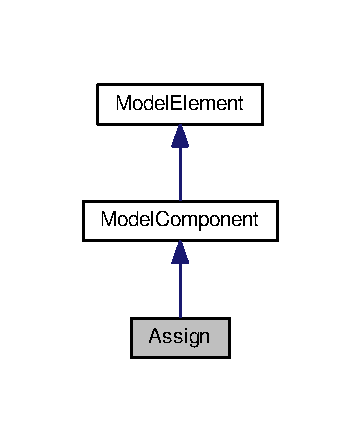
\includegraphics[width=181pt]{class_assign__inherit__graph}
\end{center}
\end{figure}


Collaboration diagram for Assign\+:
\nopagebreak
\begin{figure}[H]
\begin{center}
\leavevmode
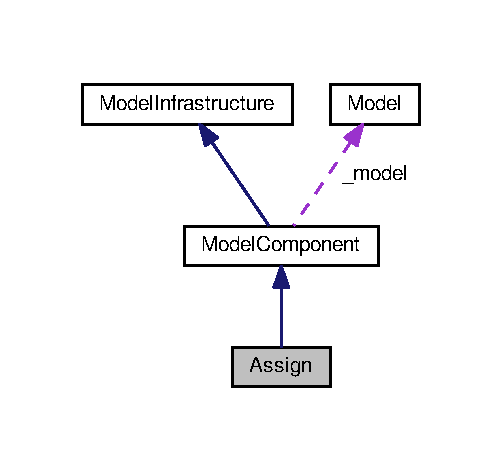
\includegraphics[width=242pt]{class_assign__coll__graph}
\end{center}
\end{figure}
\subsection*{Classes}
\begin{DoxyCompactItemize}
\item 
class \hyperlink{class_assign_1_1_assignment}{Assignment}
\end{DoxyCompactItemize}
\subsection*{Public Types}
\begin{DoxyCompactItemize}
\item 
enum \hyperlink{class_assign_ae0f42117c12a8d0bc2bf0b7574070694}{Destination\+Type} \{ \hyperlink{class_assign_ae0f42117c12a8d0bc2bf0b7574070694af2bbdf9f72c085adc4d0404e370f0f4c}{Destination\+Type\+::\+Attribute}, 
\hyperlink{class_assign_ae0f42117c12a8d0bc2bf0b7574070694a47c14840d8e15331fa420b9b2f757cd9}{Destination\+Type\+::\+Variable}
 \}
\end{DoxyCompactItemize}
\subsection*{Public Member Functions}
\begin{DoxyCompactItemize}
\item 
\hyperlink{class_assign_afaa746a0ce157d4606823ad508dc6281}{Assign} (\hyperlink{class_model}{Model} $\ast$model)
\item 
\hyperlink{class_assign_ae4945adcf1b5dcdd3f57faa9dd85a2b0}{Assign} (const \hyperlink{class_assign}{Assign} \&orig)
\item 
virtual \hyperlink{class_assign_aa005626af06022d9101c5e38e794dc47}{$\sim$\+Assign} ()
\item 
virtual std\+::string \hyperlink{class_assign_af5022b92204adcd9ee3e444b7e316d07}{show} ()
\item 
\hyperlink{class_list}{List}$<$ \hyperlink{class_assign_1_1_assignment}{Assignment} $\ast$ $>$ $\ast$ \hyperlink{class_assign_aca4aaa2185cc8770e56e1b6928c33dc0}{get\+Assignments} () const 
\end{DoxyCompactItemize}
\subsection*{Protected Member Functions}
\begin{DoxyCompactItemize}
\item 
virtual void \hyperlink{class_assign_a5fabf69268b2e65d8b01ce247be87a40}{\+\_\+execute} (\hyperlink{class_entity}{Entity} $\ast$entity)
\item 
virtual void \hyperlink{class_assign_a95e3169a6ae13ef3dc6dd9f0dde16c30}{\+\_\+load\+Instance} (std\+::list$<$ std\+::string $>$ words)
\item 
virtual std\+::list$<$ std\+::string $>$ $\ast$ \hyperlink{class_assign_a8b38a0a1bec283f5d2f44f67be5a4a6b}{\+\_\+save\+Instance} ()
\item 
virtual bool \hyperlink{class_assign_a5f3a7d8a7214574fea926cae1b1acb94}{\+\_\+verify\+Symbols} (std\+::string $\ast$error\+Message)
\end{DoxyCompactItemize}
\subsection*{Additional Inherited Members}


\subsection{Member Enumeration Documentation}
\index{Assign@{Assign}!Destination\+Type@{Destination\+Type}}
\index{Destination\+Type@{Destination\+Type}!Assign@{Assign}}
\subsubsection[{\texorpdfstring{Destination\+Type}{DestinationType}}]{\setlength{\rightskip}{0pt plus 5cm}enum {\bf Assign\+::\+Destination\+Type}\hspace{0.3cm}{\ttfamily [strong]}}\hypertarget{class_assign_ae0f42117c12a8d0bc2bf0b7574070694}{}\label{class_assign_ae0f42117c12a8d0bc2bf0b7574070694}
\begin{Desc}
\item[Enumerator]\par
\begin{description}
\index{Attribute@{Attribute}!Assign@{Assign}}\index{Assign@{Assign}!Attribute@{Attribute}}\item[{\em 
Attribute\hypertarget{class_assign_ae0f42117c12a8d0bc2bf0b7574070694af2bbdf9f72c085adc4d0404e370f0f4c}{}\label{class_assign_ae0f42117c12a8d0bc2bf0b7574070694af2bbdf9f72c085adc4d0404e370f0f4c}
}]\index{Variable@{Variable}!Assign@{Assign}}\index{Assign@{Assign}!Variable@{Variable}}\item[{\em 
Variable\hypertarget{class_assign_ae0f42117c12a8d0bc2bf0b7574070694a47c14840d8e15331fa420b9b2f757cd9}{}\label{class_assign_ae0f42117c12a8d0bc2bf0b7574070694a47c14840d8e15331fa420b9b2f757cd9}
}]\end{description}
\end{Desc}


\subsection{Constructor \& Destructor Documentation}
\index{Assign@{Assign}!Assign@{Assign}}
\index{Assign@{Assign}!Assign@{Assign}}
\subsubsection[{\texorpdfstring{Assign(\+Model $\ast$model)}{Assign(Model *model)}}]{\setlength{\rightskip}{0pt plus 5cm}Assign\+::\+Assign (
\begin{DoxyParamCaption}
\item[{{\bf Model} $\ast$}]{model}
\end{DoxyParamCaption}
)}\hypertarget{class_assign_afaa746a0ce157d4606823ad508dc6281}{}\label{class_assign_afaa746a0ce157d4606823ad508dc6281}
\index{Assign@{Assign}!Assign@{Assign}}
\index{Assign@{Assign}!Assign@{Assign}}
\subsubsection[{\texorpdfstring{Assign(const Assign \&orig)}{Assign(const Assign &orig)}}]{\setlength{\rightskip}{0pt plus 5cm}Assign\+::\+Assign (
\begin{DoxyParamCaption}
\item[{const {\bf Assign} \&}]{orig}
\end{DoxyParamCaption}
)}\hypertarget{class_assign_ae4945adcf1b5dcdd3f57faa9dd85a2b0}{}\label{class_assign_ae4945adcf1b5dcdd3f57faa9dd85a2b0}
\index{Assign@{Assign}!````~Assign@{$\sim$\+Assign}}
\index{````~Assign@{$\sim$\+Assign}!Assign@{Assign}}
\subsubsection[{\texorpdfstring{$\sim$\+Assign()}{~Assign()}}]{\setlength{\rightskip}{0pt plus 5cm}Assign\+::$\sim$\+Assign (
\begin{DoxyParamCaption}
{}
\end{DoxyParamCaption}
)\hspace{0.3cm}{\ttfamily [virtual]}}\hypertarget{class_assign_aa005626af06022d9101c5e38e794dc47}{}\label{class_assign_aa005626af06022d9101c5e38e794dc47}


\subsection{Member Function Documentation}
\index{Assign@{Assign}!\+\_\+execute@{\+\_\+execute}}
\index{\+\_\+execute@{\+\_\+execute}!Assign@{Assign}}
\subsubsection[{\texorpdfstring{\+\_\+execute(\+Entity $\ast$entity)}{_execute(Entity *entity)}}]{\setlength{\rightskip}{0pt plus 5cm}void Assign\+::\+\_\+execute (
\begin{DoxyParamCaption}
\item[{{\bf Entity} $\ast$}]{entity}
\end{DoxyParamCaption}
)\hspace{0.3cm}{\ttfamily [protected]}, {\ttfamily [virtual]}}\hypertarget{class_assign_a5fabf69268b2e65d8b01ce247be87a40}{}\label{class_assign_a5fabf69268b2e65d8b01ce247be87a40}


Implements \hyperlink{class_model_component_ae3fcf8bbdd8368c882438424aa73f714}{Model\+Component}.

\index{Assign@{Assign}!\+\_\+load\+Instance@{\+\_\+load\+Instance}}
\index{\+\_\+load\+Instance@{\+\_\+load\+Instance}!Assign@{Assign}}
\subsubsection[{\texorpdfstring{\+\_\+load\+Instance(std\+::list$<$ std\+::string $>$ words)}{_loadInstance(std::list< std::string > words)}}]{\setlength{\rightskip}{0pt plus 5cm}void Assign\+::\+\_\+load\+Instance (
\begin{DoxyParamCaption}
\item[{std\+::list$<$ std\+::string $>$}]{words}
\end{DoxyParamCaption}
)\hspace{0.3cm}{\ttfamily [protected]}, {\ttfamily [virtual]}}\hypertarget{class_assign_a95e3169a6ae13ef3dc6dd9f0dde16c30}{}\label{class_assign_a95e3169a6ae13ef3dc6dd9f0dde16c30}


Implements \hyperlink{class_model_infrastructure_ae118c8ad2ac9d4397c40d004af51b2dc}{Model\+Infrastructure}.

\index{Assign@{Assign}!\+\_\+save\+Instance@{\+\_\+save\+Instance}}
\index{\+\_\+save\+Instance@{\+\_\+save\+Instance}!Assign@{Assign}}
\subsubsection[{\texorpdfstring{\+\_\+save\+Instance()}{_saveInstance()}}]{\setlength{\rightskip}{0pt plus 5cm}std\+::list$<$ std\+::string $>$ $\ast$ Assign\+::\+\_\+save\+Instance (
\begin{DoxyParamCaption}
{}
\end{DoxyParamCaption}
)\hspace{0.3cm}{\ttfamily [protected]}, {\ttfamily [virtual]}}\hypertarget{class_assign_a8b38a0a1bec283f5d2f44f67be5a4a6b}{}\label{class_assign_a8b38a0a1bec283f5d2f44f67be5a4a6b}


Reimplemented from \hyperlink{class_model_component_a465f41c7191cb0fdf9039ef1f3d755a5}{Model\+Component}.

\index{Assign@{Assign}!\+\_\+verify\+Symbols@{\+\_\+verify\+Symbols}}
\index{\+\_\+verify\+Symbols@{\+\_\+verify\+Symbols}!Assign@{Assign}}
\subsubsection[{\texorpdfstring{\+\_\+verify\+Symbols(std\+::string $\ast$error\+Message)}{_verifySymbols(std::string *errorMessage)}}]{\setlength{\rightskip}{0pt plus 5cm}bool Assign\+::\+\_\+verify\+Symbols (
\begin{DoxyParamCaption}
\item[{std\+::string $\ast$}]{error\+Message}
\end{DoxyParamCaption}
)\hspace{0.3cm}{\ttfamily [protected]}, {\ttfamily [virtual]}}\hypertarget{class_assign_a5f3a7d8a7214574fea926cae1b1acb94}{}\label{class_assign_a5f3a7d8a7214574fea926cae1b1acb94}


Implements \hyperlink{class_model_infrastructure_a43de089b35b96c32dd24ca4f9636a388}{Model\+Infrastructure}.

\index{Assign@{Assign}!get\+Assignments@{get\+Assignments}}
\index{get\+Assignments@{get\+Assignments}!Assign@{Assign}}
\subsubsection[{\texorpdfstring{get\+Assignments() const }{getAssignments() const }}]{\setlength{\rightskip}{0pt plus 5cm}{\bf List}$<$ {\bf Assign\+::\+Assignment} $\ast$ $>$ $\ast$ Assign\+::get\+Assignments (
\begin{DoxyParamCaption}
{}
\end{DoxyParamCaption}
) const}\hypertarget{class_assign_aca4aaa2185cc8770e56e1b6928c33dc0}{}\label{class_assign_aca4aaa2185cc8770e56e1b6928c33dc0}
\index{Assign@{Assign}!show@{show}}
\index{show@{show}!Assign@{Assign}}
\subsubsection[{\texorpdfstring{show()}{show()}}]{\setlength{\rightskip}{0pt plus 5cm}std\+::string Assign\+::show (
\begin{DoxyParamCaption}
{}
\end{DoxyParamCaption}
)\hspace{0.3cm}{\ttfamily [virtual]}}\hypertarget{class_assign_af5022b92204adcd9ee3e444b7e316d07}{}\label{class_assign_af5022b92204adcd9ee3e444b7e316d07}


Reimplemented from \hyperlink{class_model_component_ad8bc846e36b028eab7efb7da6c549eca}{Model\+Component}.



The documentation for this class was generated from the following files\+:\begin{DoxyCompactItemize}
\item 
\hyperlink{_assign_8h}{Assign.\+h}\item 
\hyperlink{_assign_8cpp}{Assign.\+cpp}\end{DoxyCompactItemize}

\hypertarget{class_assign_1_1_assignment}{}\section{Assign\+:\+:Assignment Class Reference}
\label{class_assign_1_1_assignment}\index{Assign\+::\+Assignment@{Assign\+::\+Assignment}}


{\ttfamily \#include $<$Assign.\+h$>$}

\subsection*{Public Member Functions}
\begin{DoxyCompactItemize}
\item 
\hyperlink{class_assign_1_1_assignment_a41583f4bbce99b1d95f4ef067c236f7a}{Assignment} (\hyperlink{class_assign_ae0f42117c12a8d0bc2bf0b7574070694}{Destination\+Type} destination\+Type, std\+::string destination, std\+::string expression)
\item 
void \hyperlink{class_assign_1_1_assignment_a8d0c9b18c0b1258bba905b4e47a2659b}{set\+Destination} (std\+::string \+\_\+destination)
\item 
std\+::string \hyperlink{class_assign_1_1_assignment_a6cf7ecd2950dfc709985a1ede3773be8}{get\+Destination} () const 
\item 
void \hyperlink{class_assign_1_1_assignment_a9688ea3171c85ccbcdf0ed9d87ad9cc7}{set\+Destination\+Type} (\hyperlink{class_assign_ae0f42117c12a8d0bc2bf0b7574070694}{Destination\+Type} \+\_\+destination\+Type)
\item 
\hyperlink{class_assign_ae0f42117c12a8d0bc2bf0b7574070694}{Destination\+Type} \hyperlink{class_assign_1_1_assignment_a46493b98c1cd97ce4b015640bf34dd27}{get\+Destination\+Type} () const 
\item 
void \hyperlink{class_assign_1_1_assignment_aa36ca609362d3deedffbefd9cceb12e6}{set\+Expression} (std\+::string \+\_\+expression)
\item 
std\+::string \hyperlink{class_assign_1_1_assignment_a724dc03a686c4d53d57ee45b7617ae2f}{get\+Expression} () const 
\end{DoxyCompactItemize}


\subsection{Constructor \& Destructor Documentation}
\index{Assign\+::\+Assignment@{Assign\+::\+Assignment}!Assignment@{Assignment}}
\index{Assignment@{Assignment}!Assign\+::\+Assignment@{Assign\+::\+Assignment}}
\subsubsection[{\texorpdfstring{Assignment(\+Destination\+Type destination\+Type, std\+::string destination, std\+::string expression)}{Assignment(DestinationType destinationType, std::string destination, std::string expression)}}]{\setlength{\rightskip}{0pt plus 5cm}Assign\+::\+Assignment\+::\+Assignment (
\begin{DoxyParamCaption}
\item[{{\bf Destination\+Type}}]{destination\+Type, }
\item[{std\+::string}]{destination, }
\item[{std\+::string}]{expression}
\end{DoxyParamCaption}
)\hspace{0.3cm}{\ttfamily [inline]}}\hypertarget{class_assign_1_1_assignment_a41583f4bbce99b1d95f4ef067c236f7a}{}\label{class_assign_1_1_assignment_a41583f4bbce99b1d95f4ef067c236f7a}


\subsection{Member Function Documentation}
\index{Assign\+::\+Assignment@{Assign\+::\+Assignment}!get\+Destination@{get\+Destination}}
\index{get\+Destination@{get\+Destination}!Assign\+::\+Assignment@{Assign\+::\+Assignment}}
\subsubsection[{\texorpdfstring{get\+Destination() const }{getDestination() const }}]{\setlength{\rightskip}{0pt plus 5cm}std\+::string Assign\+::\+Assignment\+::get\+Destination (
\begin{DoxyParamCaption}
{}
\end{DoxyParamCaption}
) const\hspace{0.3cm}{\ttfamily [inline]}}\hypertarget{class_assign_1_1_assignment_a6cf7ecd2950dfc709985a1ede3773be8}{}\label{class_assign_1_1_assignment_a6cf7ecd2950dfc709985a1ede3773be8}
\index{Assign\+::\+Assignment@{Assign\+::\+Assignment}!get\+Destination\+Type@{get\+Destination\+Type}}
\index{get\+Destination\+Type@{get\+Destination\+Type}!Assign\+::\+Assignment@{Assign\+::\+Assignment}}
\subsubsection[{\texorpdfstring{get\+Destination\+Type() const }{getDestinationType() const }}]{\setlength{\rightskip}{0pt plus 5cm}{\bf Destination\+Type} Assign\+::\+Assignment\+::get\+Destination\+Type (
\begin{DoxyParamCaption}
{}
\end{DoxyParamCaption}
) const\hspace{0.3cm}{\ttfamily [inline]}}\hypertarget{class_assign_1_1_assignment_a46493b98c1cd97ce4b015640bf34dd27}{}\label{class_assign_1_1_assignment_a46493b98c1cd97ce4b015640bf34dd27}
\index{Assign\+::\+Assignment@{Assign\+::\+Assignment}!get\+Expression@{get\+Expression}}
\index{get\+Expression@{get\+Expression}!Assign\+::\+Assignment@{Assign\+::\+Assignment}}
\subsubsection[{\texorpdfstring{get\+Expression() const }{getExpression() const }}]{\setlength{\rightskip}{0pt plus 5cm}std\+::string Assign\+::\+Assignment\+::get\+Expression (
\begin{DoxyParamCaption}
{}
\end{DoxyParamCaption}
) const\hspace{0.3cm}{\ttfamily [inline]}}\hypertarget{class_assign_1_1_assignment_a724dc03a686c4d53d57ee45b7617ae2f}{}\label{class_assign_1_1_assignment_a724dc03a686c4d53d57ee45b7617ae2f}
\index{Assign\+::\+Assignment@{Assign\+::\+Assignment}!set\+Destination@{set\+Destination}}
\index{set\+Destination@{set\+Destination}!Assign\+::\+Assignment@{Assign\+::\+Assignment}}
\subsubsection[{\texorpdfstring{set\+Destination(std\+::string \+\_\+destination)}{setDestination(std::string _destination)}}]{\setlength{\rightskip}{0pt plus 5cm}void Assign\+::\+Assignment\+::set\+Destination (
\begin{DoxyParamCaption}
\item[{std\+::string}]{\+\_\+destination}
\end{DoxyParamCaption}
)\hspace{0.3cm}{\ttfamily [inline]}}\hypertarget{class_assign_1_1_assignment_a8d0c9b18c0b1258bba905b4e47a2659b}{}\label{class_assign_1_1_assignment_a8d0c9b18c0b1258bba905b4e47a2659b}
\index{Assign\+::\+Assignment@{Assign\+::\+Assignment}!set\+Destination\+Type@{set\+Destination\+Type}}
\index{set\+Destination\+Type@{set\+Destination\+Type}!Assign\+::\+Assignment@{Assign\+::\+Assignment}}
\subsubsection[{\texorpdfstring{set\+Destination\+Type(\+Destination\+Type \+\_\+destination\+Type)}{setDestinationType(DestinationType _destinationType)}}]{\setlength{\rightskip}{0pt plus 5cm}void Assign\+::\+Assignment\+::set\+Destination\+Type (
\begin{DoxyParamCaption}
\item[{{\bf Destination\+Type}}]{\+\_\+destination\+Type}
\end{DoxyParamCaption}
)\hspace{0.3cm}{\ttfamily [inline]}}\hypertarget{class_assign_1_1_assignment_a9688ea3171c85ccbcdf0ed9d87ad9cc7}{}\label{class_assign_1_1_assignment_a9688ea3171c85ccbcdf0ed9d87ad9cc7}
\index{Assign\+::\+Assignment@{Assign\+::\+Assignment}!set\+Expression@{set\+Expression}}
\index{set\+Expression@{set\+Expression}!Assign\+::\+Assignment@{Assign\+::\+Assignment}}
\subsubsection[{\texorpdfstring{set\+Expression(std\+::string \+\_\+expression)}{setExpression(std::string _expression)}}]{\setlength{\rightskip}{0pt plus 5cm}void Assign\+::\+Assignment\+::set\+Expression (
\begin{DoxyParamCaption}
\item[{std\+::string}]{\+\_\+expression}
\end{DoxyParamCaption}
)\hspace{0.3cm}{\ttfamily [inline]}}\hypertarget{class_assign_1_1_assignment_aa36ca609362d3deedffbefd9cceb12e6}{}\label{class_assign_1_1_assignment_aa36ca609362d3deedffbefd9cceb12e6}


The documentation for this class was generated from the following file\+:\begin{DoxyCompactItemize}
\item 
\hyperlink{_assign_8h}{Assign.\+h}\end{DoxyCompactItemize}

\hypertarget{class_attribute}{\section{Attribute Class Reference}
\label{class_attribute}\index{Attribute@{Attribute}}
}


{\ttfamily \#include $<$Attribute.\-h$>$}



Inheritance diagram for Attribute\-:
\nopagebreak
\begin{figure}[H]
\begin{center}
\leavevmode
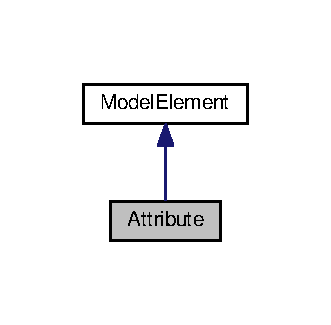
\includegraphics[width=180pt]{class_attribute__inherit__graph}
\end{center}
\end{figure}


Collaboration diagram for Attribute\-:
\nopagebreak
\begin{figure}[H]
\begin{center}
\leavevmode
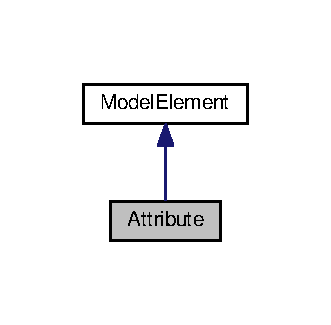
\includegraphics[width=180pt]{class_attribute__coll__graph}
\end{center}
\end{figure}
\subsection*{Public Member Functions}
\begin{DoxyCompactItemize}
\item 
\hyperlink{class_attribute_a8ba4e5a507aef352563e1e56f1930e66}{Attribute} ()
\item 
\hyperlink{class_attribute_a8a0c53bda9cc94180f06bda254809261}{Attribute} (const \hyperlink{class_attribute}{Attribute} \&orig)
\item 
virtual \hyperlink{class_attribute_a28ab087bb886728670e4ae5791bc2ea8}{$\sim$\-Attribute} ()
\item 
virtual std\-::string \hyperlink{class_attribute_aa29f79466bd6ed5e36c402ec57cb2050}{show} ()
\end{DoxyCompactItemize}
\subsection*{Protected Member Functions}
\begin{DoxyCompactItemize}
\item 
virtual void \hyperlink{class_attribute_ac76d3302ec24a4cca1e84fed221cf917}{\-\_\-load\-Instance} (std\-::list$<$ std\-::string $>$ words)
\item 
virtual std\-::list$<$ std\-::string $>$ $\ast$ \hyperlink{class_attribute_a32bd3d820fa2957d4a5d8c98db5b50e0}{\-\_\-save\-Instance} ()
\item 
virtual bool \hyperlink{class_attribute_adbe1f438203db4e87b0c8e1cd5e0182d}{\-\_\-verify\-Symbols} (std\-::string $\ast$error\-Message)
\end{DoxyCompactItemize}
\subsection*{Additional Inherited Members}


\subsection{Detailed Description}


Definition at line 24 of file Attribute.\-h.



\subsection{Constructor \& Destructor Documentation}
\hypertarget{class_attribute_a8ba4e5a507aef352563e1e56f1930e66}{\index{Attribute@{Attribute}!Attribute@{Attribute}}
\index{Attribute@{Attribute}!Attribute@{Attribute}}
\subsubsection[{Attribute}]{\setlength{\rightskip}{0pt plus 5cm}Attribute\-::\-Attribute (
\begin{DoxyParamCaption}
{}
\end{DoxyParamCaption}
)}}\label{class_attribute_a8ba4e5a507aef352563e1e56f1930e66}


Definition at line 16 of file Attribute.\-cpp.

\hypertarget{class_attribute_a8a0c53bda9cc94180f06bda254809261}{\index{Attribute@{Attribute}!Attribute@{Attribute}}
\index{Attribute@{Attribute}!Attribute@{Attribute}}
\subsubsection[{Attribute}]{\setlength{\rightskip}{0pt plus 5cm}Attribute\-::\-Attribute (
\begin{DoxyParamCaption}
\item[{const {\bf Attribute} \&}]{orig}
\end{DoxyParamCaption}
)}}\label{class_attribute_a8a0c53bda9cc94180f06bda254809261}


Definition at line 19 of file Attribute.\-cpp.

\hypertarget{class_attribute_a28ab087bb886728670e4ae5791bc2ea8}{\index{Attribute@{Attribute}!$\sim$\-Attribute@{$\sim$\-Attribute}}
\index{$\sim$\-Attribute@{$\sim$\-Attribute}!Attribute@{Attribute}}
\subsubsection[{$\sim$\-Attribute}]{\setlength{\rightskip}{0pt plus 5cm}Attribute\-::$\sim$\-Attribute (
\begin{DoxyParamCaption}
{}
\end{DoxyParamCaption}
)\hspace{0.3cm}{\ttfamily [virtual]}}}\label{class_attribute_a28ab087bb886728670e4ae5791bc2ea8}


Definition at line 22 of file Attribute.\-cpp.



\subsection{Member Function Documentation}
\hypertarget{class_attribute_ac76d3302ec24a4cca1e84fed221cf917}{\index{Attribute@{Attribute}!\-\_\-load\-Instance@{\-\_\-load\-Instance}}
\index{\-\_\-load\-Instance@{\-\_\-load\-Instance}!Attribute@{Attribute}}
\subsubsection[{\-\_\-load\-Instance}]{\setlength{\rightskip}{0pt plus 5cm}void Attribute\-::\-\_\-load\-Instance (
\begin{DoxyParamCaption}
\item[{std\-::list$<$ std\-::string $>$}]{words}
\end{DoxyParamCaption}
)\hspace{0.3cm}{\ttfamily [protected]}, {\ttfamily [virtual]}}}\label{class_attribute_ac76d3302ec24a4cca1e84fed221cf917}


Implements \hyperlink{class_model_infrastructure_ae118c8ad2ac9d4397c40d004af51b2dc}{Model\-Infrastructure}.



Definition at line 29 of file Attribute.\-cpp.

\hypertarget{class_attribute_a32bd3d820fa2957d4a5d8c98db5b50e0}{\index{Attribute@{Attribute}!\-\_\-save\-Instance@{\-\_\-save\-Instance}}
\index{\-\_\-save\-Instance@{\-\_\-save\-Instance}!Attribute@{Attribute}}
\subsubsection[{\-\_\-save\-Instance}]{\setlength{\rightskip}{0pt plus 5cm}std\-::list$<$ std\-::string $>$ $\ast$ Attribute\-::\-\_\-save\-Instance (
\begin{DoxyParamCaption}
{}
\end{DoxyParamCaption}
)\hspace{0.3cm}{\ttfamily [protected]}, {\ttfamily [virtual]}}}\label{class_attribute_a32bd3d820fa2957d4a5d8c98db5b50e0}


Implements \hyperlink{class_model_infrastructure_a3da2fd381c44752598bc448b207e8287}{Model\-Infrastructure}.



Definition at line 32 of file Attribute.\-cpp.

\hypertarget{class_attribute_adbe1f438203db4e87b0c8e1cd5e0182d}{\index{Attribute@{Attribute}!\-\_\-verify\-Symbols@{\-\_\-verify\-Symbols}}
\index{\-\_\-verify\-Symbols@{\-\_\-verify\-Symbols}!Attribute@{Attribute}}
\subsubsection[{\-\_\-verify\-Symbols}]{\setlength{\rightskip}{0pt plus 5cm}bool Attribute\-::\-\_\-verify\-Symbols (
\begin{DoxyParamCaption}
\item[{std\-::string $\ast$}]{error\-Message}
\end{DoxyParamCaption}
)\hspace{0.3cm}{\ttfamily [protected]}, {\ttfamily [virtual]}}}\label{class_attribute_adbe1f438203db4e87b0c8e1cd5e0182d}


Implements \hyperlink{class_model_infrastructure_a43de089b35b96c32dd24ca4f9636a388}{Model\-Infrastructure}.



Definition at line 37 of file Attribute.\-cpp.

\hypertarget{class_attribute_aa29f79466bd6ed5e36c402ec57cb2050}{\index{Attribute@{Attribute}!show@{show}}
\index{show@{show}!Attribute@{Attribute}}
\subsubsection[{show}]{\setlength{\rightskip}{0pt plus 5cm}std\-::string Attribute\-::show (
\begin{DoxyParamCaption}
{}
\end{DoxyParamCaption}
)\hspace{0.3cm}{\ttfamily [virtual]}}}\label{class_attribute_aa29f79466bd6ed5e36c402ec57cb2050}


Reimplemented from \hyperlink{class_model_infrastructure_a649a5a89a0c9931783d3c51de2acf266}{Model\-Infrastructure}.



Definition at line 25 of file Attribute.\-cpp.



Here is the call graph for this function\-:
\nopagebreak
\begin{figure}[H]
\begin{center}
\leavevmode
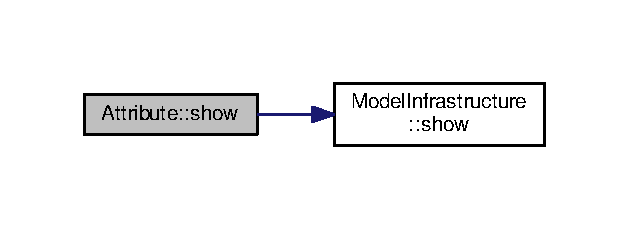
\includegraphics[width=302pt]{class_attribute_aa29f79466bd6ed5e36c402ec57cb2050_cgraph}
\end{center}
\end{figure}




The documentation for this class was generated from the following files\-:\begin{DoxyCompactItemize}
\item 
\hyperlink{_attribute_8h}{Attribute.\-h}\item 
\hyperlink{_attribute_8cpp}{Attribute.\-cpp}\end{DoxyCompactItemize}

\hypertarget{class_build_simulation_model}{\section{Build\-Simulation\-Model Class Reference}
\label{class_build_simulation_model}\index{Build\-Simulation\-Model@{Build\-Simulation\-Model}}
}


{\ttfamily \#include $<$Build\-Simulation\-Model.\-h$>$}



Inheritance diagram for Build\-Simulation\-Model\-:
\nopagebreak
\begin{figure}[H]
\begin{center}
\leavevmode
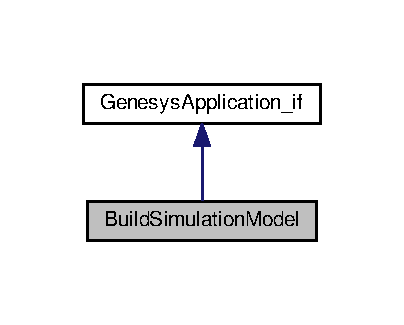
\includegraphics[width=194pt]{class_build_simulation_model__inherit__graph}
\end{center}
\end{figure}


Collaboration diagram for Build\-Simulation\-Model\-:
\nopagebreak
\begin{figure}[H]
\begin{center}
\leavevmode
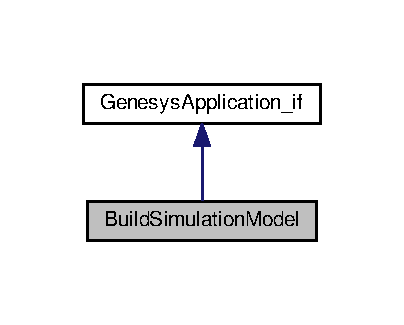
\includegraphics[width=194pt]{class_build_simulation_model__coll__graph}
\end{center}
\end{figure}
\subsection*{Public Member Functions}
\begin{DoxyCompactItemize}
\item 
\hyperlink{class_build_simulation_model_a477872592a89845e00cfbc7b6063bb21}{Build\-Simulation\-Model} ()
\item 
int \hyperlink{class_build_simulation_model_a8c50f55d7293860e5e7bc7e7e74f8d4a}{main} (int argc, char $\ast$$\ast$argv)
\end{DoxyCompactItemize}


\subsection{Detailed Description}


Definition at line 19 of file Build\-Simulation\-Model.\-h.



\subsection{Constructor \& Destructor Documentation}
\hypertarget{class_build_simulation_model_a477872592a89845e00cfbc7b6063bb21}{\index{Build\-Simulation\-Model@{Build\-Simulation\-Model}!Build\-Simulation\-Model@{Build\-Simulation\-Model}}
\index{Build\-Simulation\-Model@{Build\-Simulation\-Model}!BuildSimulationModel@{Build\-Simulation\-Model}}
\subsubsection[{Build\-Simulation\-Model}]{\setlength{\rightskip}{0pt plus 5cm}Build\-Simulation\-Model\-::\-Build\-Simulation\-Model (
\begin{DoxyParamCaption}
{}
\end{DoxyParamCaption}
)}}\label{class_build_simulation_model_a477872592a89845e00cfbc7b6063bb21}


Definition at line 102 of file Build\-Simulation\-Model.\-cpp.



\subsection{Member Function Documentation}
\hypertarget{class_build_simulation_model_a8c50f55d7293860e5e7bc7e7e74f8d4a}{\index{Build\-Simulation\-Model@{Build\-Simulation\-Model}!main@{main}}
\index{main@{main}!BuildSimulationModel@{Build\-Simulation\-Model}}
\subsubsection[{main}]{\setlength{\rightskip}{0pt plus 5cm}int Build\-Simulation\-Model\-::main (
\begin{DoxyParamCaption}
\item[{int}]{argc, }
\item[{char $\ast$$\ast$}]{argv}
\end{DoxyParamCaption}
)\hspace{0.3cm}{\ttfamily [virtual]}}}\label{class_build_simulation_model_a8c50f55d7293860e5e7bc7e7e74f8d4a}


Implements \hyperlink{class_genesys_application__if_a2b07e7803b410a4a8d0f87422dabb004}{Genesys\-Application\-\_\-if}.



Definition at line 117 of file Build\-Simulation\-Model.\-cpp.



Here is the call graph for this function\-:
\nopagebreak
\begin{figure}[H]
\begin{center}
\leavevmode
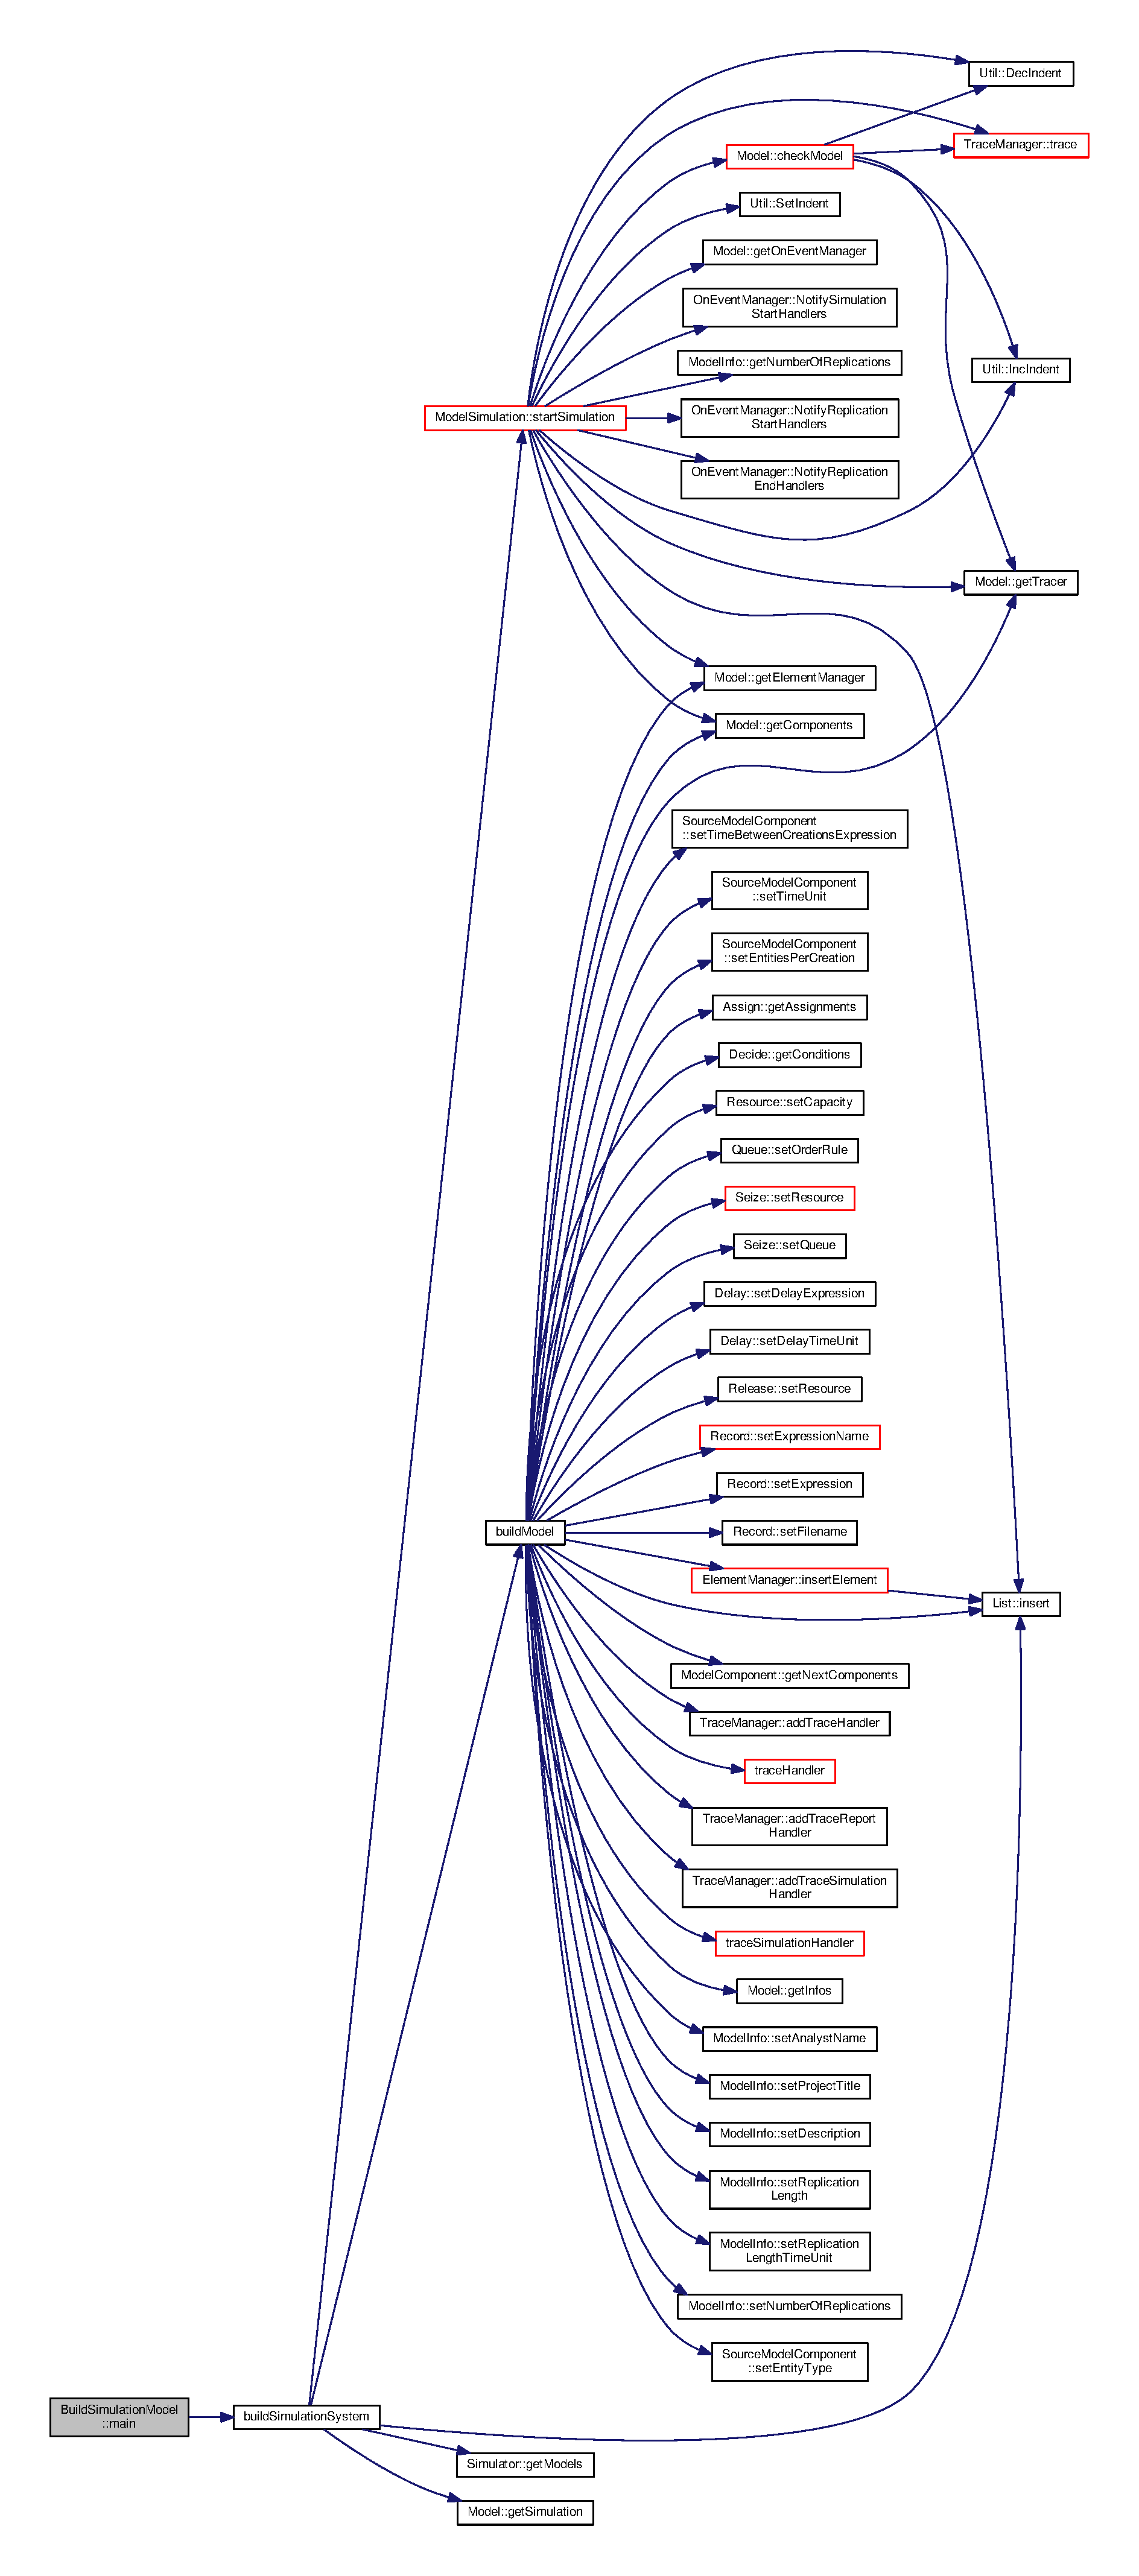
\includegraphics[height=550pt]{class_build_simulation_model_a8c50f55d7293860e5e7bc7e7e74f8d4a_cgraph}
\end{center}
\end{figure}




The documentation for this class was generated from the following files\-:\begin{DoxyCompactItemize}
\item 
\hyperlink{_build_simulation_model_8h}{Build\-Simulation\-Model.\-h}\item 
\hyperlink{_build_simulation_model_8cpp}{Build\-Simulation\-Model.\-cpp}\end{DoxyCompactItemize}

\hypertarget{class_collector__if}{\section{Collector\-\_\-if Class Reference}
\label{class_collector__if}\index{Collector\-\_\-if@{Collector\-\_\-if}}
}


{\ttfamily \#include $<$Collector\-\_\-if.\-h$>$}



Inheritance diagram for Collector\-\_\-if\-:\nopagebreak
\begin{figure}[H]
\begin{center}
\leavevmode
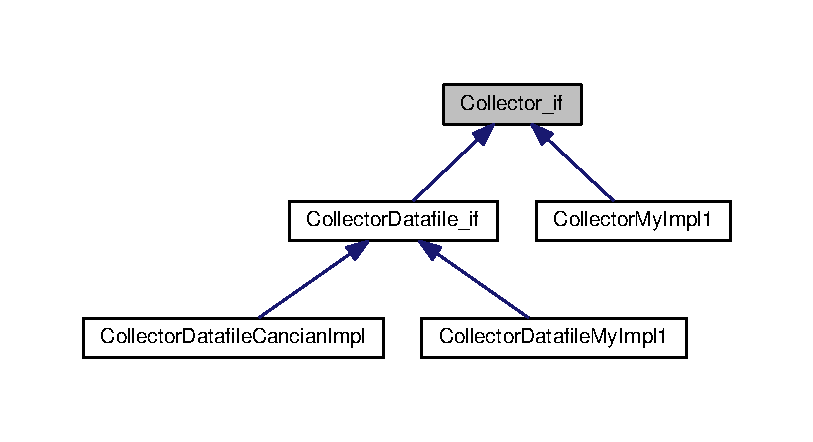
\includegraphics[width=350pt]{class_collector__if__inherit__graph}
\end{center}
\end{figure}
\subsection*{Public Member Functions}
\begin{DoxyCompactItemize}
\item 
virtual void \hyperlink{class_collector__if_a035bd1300c85866870c2f6178a9528e8}{clear} ()=0
\item 
virtual void \hyperlink{class_collector__if_ac7b83bce8ddb4903d247c1eddd656171}{add\-Value} (double value)=0
\item 
virtual double \hyperlink{class_collector__if_aa14f7e1065af8fd38ab592e224fb7e43}{get\-Last\-Value} ()=0
\item 
virtual unsigned long \hyperlink{class_collector__if_a97fa632508ffdfad1365b3a949acf745}{num\-Elements} ()=0
\end{DoxyCompactItemize}


\subsection{Detailed Description}
Interface for collecting values of a single stochastic variable. Values collected can be used as base for statistical analysis. 

Definition at line 22 of file Collector\-\_\-if.\-h.



\subsection{Member Function Documentation}
\hypertarget{class_collector__if_ac7b83bce8ddb4903d247c1eddd656171}{\index{Collector\-\_\-if@{Collector\-\_\-if}!add\-Value@{add\-Value}}
\index{add\-Value@{add\-Value}!Collector_if@{Collector\-\_\-if}}
\subsubsection[{add\-Value}]{\setlength{\rightskip}{0pt plus 5cm}virtual void Collector\-\_\-if\-::add\-Value (
\begin{DoxyParamCaption}
\item[{double}]{value}
\end{DoxyParamCaption}
)\hspace{0.3cm}{\ttfamily [pure virtual]}}}\label{class_collector__if_ac7b83bce8ddb4903d247c1eddd656171}


Implemented in \hyperlink{class_collector_datafile_cancian_impl_ab6a718100f5bdd04e3fef9edf23045ec}{Collector\-Datafile\-Cancian\-Impl}, \hyperlink{class_collector_my_impl1_acc5d658a3429af8b7d4265cbc37485b5}{Collector\-My\-Impl1}, and \hyperlink{class_collector_datafile_my_impl1_aa909fc87f2ee082512616840c9031365}{Collector\-Datafile\-My\-Impl1}.



Here is the caller graph for this function\-:\nopagebreak
\begin{figure}[H]
\begin{center}
\leavevmode
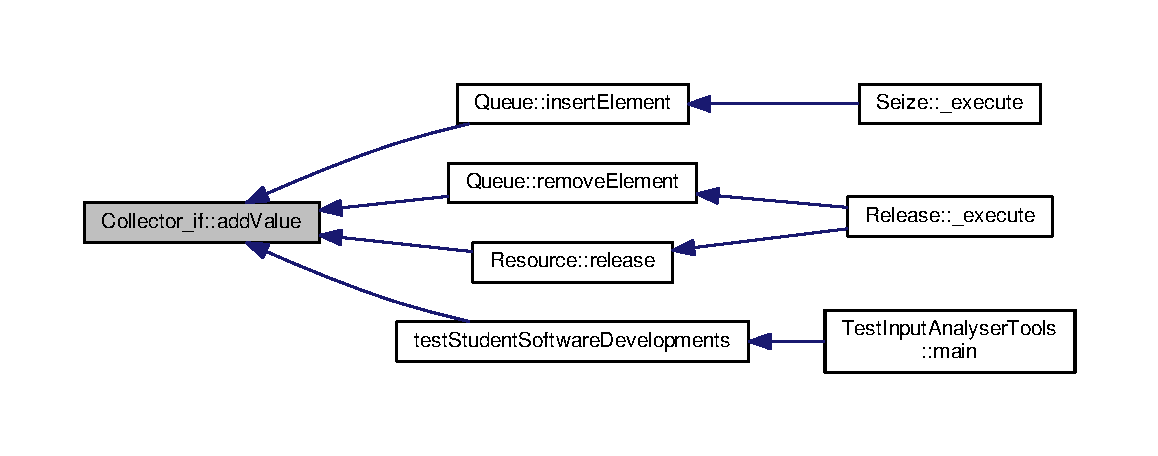
\includegraphics[width=350pt]{class_collector__if_ac7b83bce8ddb4903d247c1eddd656171_icgraph}
\end{center}
\end{figure}


\hypertarget{class_collector__if_a035bd1300c85866870c2f6178a9528e8}{\index{Collector\-\_\-if@{Collector\-\_\-if}!clear@{clear}}
\index{clear@{clear}!Collector_if@{Collector\-\_\-if}}
\subsubsection[{clear}]{\setlength{\rightskip}{0pt plus 5cm}virtual void Collector\-\_\-if\-::clear (
\begin{DoxyParamCaption}
{}
\end{DoxyParamCaption}
)\hspace{0.3cm}{\ttfamily [pure virtual]}}}\label{class_collector__if_a035bd1300c85866870c2f6178a9528e8}


Implemented in \hyperlink{class_collector_datafile_cancian_impl_a9fe0e4e764f1cc868d9c91bc68ff0ed8}{Collector\-Datafile\-Cancian\-Impl}, \hyperlink{class_collector_my_impl1_a9b570931955cafde878d6734aa914039}{Collector\-My\-Impl1}, and \hyperlink{class_collector_datafile_my_impl1_a594004f005db5dd1122946445f4db70d}{Collector\-Datafile\-My\-Impl1}.

\hypertarget{class_collector__if_aa14f7e1065af8fd38ab592e224fb7e43}{\index{Collector\-\_\-if@{Collector\-\_\-if}!get\-Last\-Value@{get\-Last\-Value}}
\index{get\-Last\-Value@{get\-Last\-Value}!Collector_if@{Collector\-\_\-if}}
\subsubsection[{get\-Last\-Value}]{\setlength{\rightskip}{0pt plus 5cm}virtual double Collector\-\_\-if\-::get\-Last\-Value (
\begin{DoxyParamCaption}
{}
\end{DoxyParamCaption}
)\hspace{0.3cm}{\ttfamily [pure virtual]}}}\label{class_collector__if_aa14f7e1065af8fd38ab592e224fb7e43}


Implemented in \hyperlink{class_collector_datafile_cancian_impl_a24b93dedb5f56e710e810c05e89dc36f}{Collector\-Datafile\-Cancian\-Impl}, \hyperlink{class_collector_my_impl1_a56e754ba3175e2f335290e2a737e7104}{Collector\-My\-Impl1}, and \hyperlink{class_collector_datafile_my_impl1_a5a29b2f71a4630c658fb83c047fb1054}{Collector\-Datafile\-My\-Impl1}.

\hypertarget{class_collector__if_a97fa632508ffdfad1365b3a949acf745}{\index{Collector\-\_\-if@{Collector\-\_\-if}!num\-Elements@{num\-Elements}}
\index{num\-Elements@{num\-Elements}!Collector_if@{Collector\-\_\-if}}
\subsubsection[{num\-Elements}]{\setlength{\rightskip}{0pt plus 5cm}virtual unsigned long Collector\-\_\-if\-::num\-Elements (
\begin{DoxyParamCaption}
{}
\end{DoxyParamCaption}
)\hspace{0.3cm}{\ttfamily [pure virtual]}}}\label{class_collector__if_a97fa632508ffdfad1365b3a949acf745}


Implemented in \hyperlink{class_collector_datafile_cancian_impl_ab10e682e4b991a881efb56caebb4efa9}{Collector\-Datafile\-Cancian\-Impl}, \hyperlink{class_collector_my_impl1_a25427d84682943e0f588d494c54f79d8}{Collector\-My\-Impl1}, and \hyperlink{class_collector_datafile_my_impl1_ac8ad59a3b664d082c8ca4fca9887148a}{Collector\-Datafile\-My\-Impl1}.



The documentation for this class was generated from the following file\-:\begin{DoxyCompactItemize}
\item 
\hyperlink{_collector__if_8h}{Collector\-\_\-if.\-h}\end{DoxyCompactItemize}

\hypertarget{class_collector_datafile__if}{\section{Collector\-Datafile\-\_\-if Class Reference}
\label{class_collector_datafile__if}\index{Collector\-Datafile\-\_\-if@{Collector\-Datafile\-\_\-if}}
}


{\ttfamily \#include $<$Collector\-Datafile\-\_\-if.\-h$>$}



Inheritance diagram for Collector\-Datafile\-\_\-if\-:
\nopagebreak
\begin{figure}[H]
\begin{center}
\leavevmode
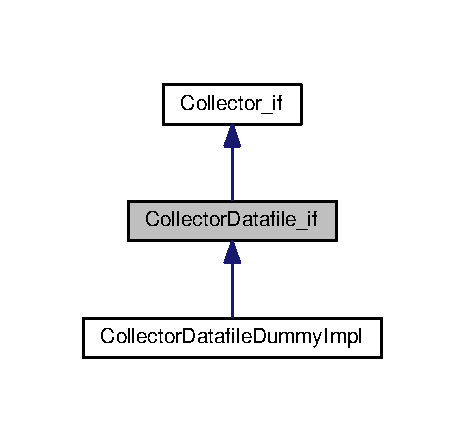
\includegraphics[width=206pt]{class_collector_datafile__if__inherit__graph}
\end{center}
\end{figure}


Collaboration diagram for Collector\-Datafile\-\_\-if\-:
\nopagebreak
\begin{figure}[H]
\begin{center}
\leavevmode
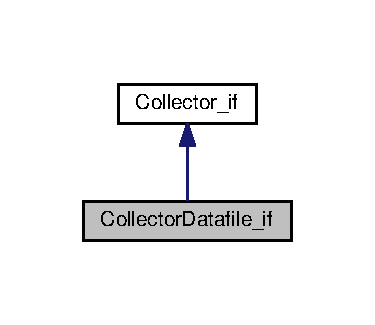
\includegraphics[width=180pt]{class_collector_datafile__if__coll__graph}
\end{center}
\end{figure}
\subsection*{Public Member Functions}
\begin{DoxyCompactItemize}
\item 
virtual double \hyperlink{class_collector_datafile__if_aa790efe68dfa16cebd66b481bbda8411}{get\-Value} (unsigned int num)=0
\item 
virtual std\-::string \hyperlink{class_collector_datafile__if_a81d109f34c25f5295f76ba13f4234a3c}{get\-Data\-Filename} ()=0
\item 
virtual void \hyperlink{class_collector_datafile__if_ab826bbf5472a5cfdbf2f2c30273da8eb}{set\-Data\-Filename} (std\-::string filename)=0
\end{DoxyCompactItemize}


\subsection{Member Function Documentation}
\hypertarget{class_collector_datafile__if_a81d109f34c25f5295f76ba13f4234a3c}{\index{Collector\-Datafile\-\_\-if@{Collector\-Datafile\-\_\-if}!get\-Data\-Filename@{get\-Data\-Filename}}
\index{get\-Data\-Filename@{get\-Data\-Filename}!CollectorDatafile_if@{Collector\-Datafile\-\_\-if}}
\subsubsection[{get\-Data\-Filename}]{\setlength{\rightskip}{0pt plus 5cm}virtual std\-::string Collector\-Datafile\-\_\-if\-::get\-Data\-Filename (
\begin{DoxyParamCaption}
{}
\end{DoxyParamCaption}
)\hspace{0.3cm}{\ttfamily [pure virtual]}}}\label{class_collector_datafile__if_a81d109f34c25f5295f76ba13f4234a3c}


Implemented in \hyperlink{class_collector_datafile_my_impl1_a5ebe8076b9eb9816a1b7d823943102cf}{Collector\-Datafile\-My\-Impl1}.

\hypertarget{class_collector_datafile__if_aa790efe68dfa16cebd66b481bbda8411}{\index{Collector\-Datafile\-\_\-if@{Collector\-Datafile\-\_\-if}!get\-Value@{get\-Value}}
\index{get\-Value@{get\-Value}!CollectorDatafile_if@{Collector\-Datafile\-\_\-if}}
\subsubsection[{get\-Value}]{\setlength{\rightskip}{0pt plus 5cm}virtual double Collector\-Datafile\-\_\-if\-::get\-Value (
\begin{DoxyParamCaption}
\item[{unsigned int}]{num}
\end{DoxyParamCaption}
)\hspace{0.3cm}{\ttfamily [pure virtual]}}}\label{class_collector_datafile__if_aa790efe68dfa16cebd66b481bbda8411}


Implemented in \hyperlink{class_collector_datafile_my_impl1_a55a505d56f9b95a55473bdf1ab24cffe}{Collector\-Datafile\-My\-Impl1}.

\hypertarget{class_collector_datafile__if_ab826bbf5472a5cfdbf2f2c30273da8eb}{\index{Collector\-Datafile\-\_\-if@{Collector\-Datafile\-\_\-if}!set\-Data\-Filename@{set\-Data\-Filename}}
\index{set\-Data\-Filename@{set\-Data\-Filename}!CollectorDatafile_if@{Collector\-Datafile\-\_\-if}}
\subsubsection[{set\-Data\-Filename}]{\setlength{\rightskip}{0pt plus 5cm}virtual void Collector\-Datafile\-\_\-if\-::set\-Data\-Filename (
\begin{DoxyParamCaption}
\item[{std\-::string}]{filename}
\end{DoxyParamCaption}
)\hspace{0.3cm}{\ttfamily [pure virtual]}}}\label{class_collector_datafile__if_ab826bbf5472a5cfdbf2f2c30273da8eb}


Implemented in \hyperlink{class_collector_datafile_my_impl1_ac4c401ae3cf4ccc723b6b9efa614ccd1}{Collector\-Datafile\-My\-Impl1}.



The documentation for this class was generated from the following file\-:\begin{DoxyCompactItemize}
\item 
\hyperlink{_collector_datafile__if_8h}{Collector\-Datafile\-\_\-if.\-h}\end{DoxyCompactItemize}

\hypertarget{class_collector_datafile_default_impl1}{}\section{Collector\+Datafile\+Default\+Impl1 Class Reference}
\label{class_collector_datafile_default_impl1}\index{Collector\+Datafile\+Default\+Impl1@{Collector\+Datafile\+Default\+Impl1}}


{\ttfamily \#include $<$Collector\+Datafile\+Default\+Impl1.\+h$>$}



Inheritance diagram for Collector\+Datafile\+Default\+Impl1\+:\nopagebreak
\begin{figure}[H]
\begin{center}
\leavevmode
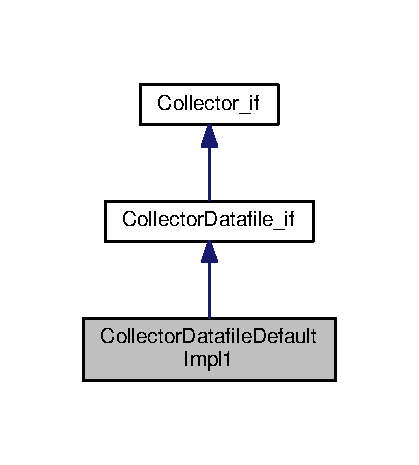
\includegraphics[width=201pt]{class_collector_datafile_default_impl1__inherit__graph}
\end{center}
\end{figure}


Collaboration diagram for Collector\+Datafile\+Default\+Impl1\+:\nopagebreak
\begin{figure}[H]
\begin{center}
\leavevmode
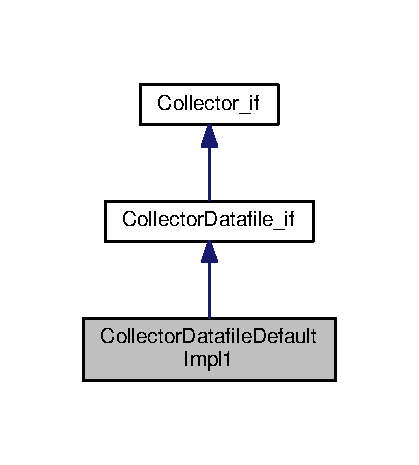
\includegraphics[width=201pt]{class_collector_datafile_default_impl1__coll__graph}
\end{center}
\end{figure}
\subsection*{Public Member Functions}
\begin{DoxyCompactItemize}
\item 
\hyperlink{class_collector_datafile_default_impl1_a4bbd717c648b3d5f87a19b01698d87c4}{Collector\+Datafile\+Default\+Impl1} ()
\item 
\hyperlink{class_collector_datafile_default_impl1_a7632b6ce3ad9d28fe2c731a7455ff40d}{Collector\+Datafile\+Default\+Impl1} (const \hyperlink{class_collector_datafile_default_impl1}{Collector\+Datafile\+Default\+Impl1} \&orig)
\item 
virtual \hyperlink{class_collector_datafile_default_impl1_a774b493b35d3fbde63e5b6458b03c772}{$\sim$\+Collector\+Datafile\+Default\+Impl1} ()
\item 
void \hyperlink{class_collector_datafile_default_impl1_aa84fa9593fd46ff37e91147aa43f71c9}{clear} ()
\item 
void \hyperlink{class_collector_datafile_default_impl1_a79de52a90a2c428ca59812f046b34ae4}{add\+Value} (double value)
\item 
double \hyperlink{class_collector_datafile_default_impl1_a453988253db1796199b41c28162c8009}{get\+Last\+Value} ()
\item 
unsigned long \hyperlink{class_collector_datafile_default_impl1_a485e0be4646bbde54578b145f3735983}{num\+Elements} ()
\item 
double \hyperlink{class_collector_datafile_default_impl1_ac40e05b78e9fcc41c648664a9597d30c}{get\+Value} (unsigned int num)
\item 
double \hyperlink{class_collector_datafile_default_impl1_a615090f649ddd8260b1f058f6cd29668}{get\+Next\+Value} ()
\item 
void \hyperlink{class_collector_datafile_default_impl1_ad8ddefdc93c51945922ea73af95def05}{seek\+First\+Value} ()
\item 
std\+::string \hyperlink{class_collector_datafile_default_impl1_afe570b0792bf13a06ff1dea12d7593b7}{get\+Data\+Filename} ()
\item 
void \hyperlink{class_collector_datafile_default_impl1_a62352f75a7635654108bb2b8b9604e1d}{set\+Data\+Filename} (std\+::string filename)
\item 
void \hyperlink{class_collector_datafile_default_impl1_adad90926a028e08397aaafa05ae643c6}{set\+Add\+Value\+Handler} (\hyperlink{_collector__if_8h_ab97c9a368c50eb9e00cb4772e46ff38a}{Collector\+Add\+Value\+Handler} add\+Value\+Handler)
\item 
void \hyperlink{class_collector_datafile_default_impl1_ae4aae3cbd96ebec268c931bd7a0a57a5}{set\+Clear\+Handler} (\hyperlink{_collector__if_8h_ad22205bb584ed3e0db55fc265a5fe1f4}{Collector\+Clear\+Handler} clear\+Handler)
\end{DoxyCompactItemize}


\subsection{Constructor \& Destructor Documentation}
\index{Collector\+Datafile\+Default\+Impl1@{Collector\+Datafile\+Default\+Impl1}!Collector\+Datafile\+Default\+Impl1@{Collector\+Datafile\+Default\+Impl1}}
\index{Collector\+Datafile\+Default\+Impl1@{Collector\+Datafile\+Default\+Impl1}!Collector\+Datafile\+Default\+Impl1@{Collector\+Datafile\+Default\+Impl1}}
\subsubsection[{\texorpdfstring{Collector\+Datafile\+Default\+Impl1()}{CollectorDatafileDefaultImpl1()}}]{\setlength{\rightskip}{0pt plus 5cm}Collector\+Datafile\+Default\+Impl1\+::\+Collector\+Datafile\+Default\+Impl1 (
\begin{DoxyParamCaption}
{}
\end{DoxyParamCaption}
)}\hypertarget{class_collector_datafile_default_impl1_a4bbd717c648b3d5f87a19b01698d87c4}{}\label{class_collector_datafile_default_impl1_a4bbd717c648b3d5f87a19b01698d87c4}
\index{Collector\+Datafile\+Default\+Impl1@{Collector\+Datafile\+Default\+Impl1}!Collector\+Datafile\+Default\+Impl1@{Collector\+Datafile\+Default\+Impl1}}
\index{Collector\+Datafile\+Default\+Impl1@{Collector\+Datafile\+Default\+Impl1}!Collector\+Datafile\+Default\+Impl1@{Collector\+Datafile\+Default\+Impl1}}
\subsubsection[{\texorpdfstring{Collector\+Datafile\+Default\+Impl1(const Collector\+Datafile\+Default\+Impl1 \&orig)}{CollectorDatafileDefaultImpl1(const CollectorDatafileDefaultImpl1 &orig)}}]{\setlength{\rightskip}{0pt plus 5cm}Collector\+Datafile\+Default\+Impl1\+::\+Collector\+Datafile\+Default\+Impl1 (
\begin{DoxyParamCaption}
\item[{const {\bf Collector\+Datafile\+Default\+Impl1} \&}]{orig}
\end{DoxyParamCaption}
)}\hypertarget{class_collector_datafile_default_impl1_a7632b6ce3ad9d28fe2c731a7455ff40d}{}\label{class_collector_datafile_default_impl1_a7632b6ce3ad9d28fe2c731a7455ff40d}
\index{Collector\+Datafile\+Default\+Impl1@{Collector\+Datafile\+Default\+Impl1}!````~Collector\+Datafile\+Default\+Impl1@{$\sim$\+Collector\+Datafile\+Default\+Impl1}}
\index{````~Collector\+Datafile\+Default\+Impl1@{$\sim$\+Collector\+Datafile\+Default\+Impl1}!Collector\+Datafile\+Default\+Impl1@{Collector\+Datafile\+Default\+Impl1}}
\subsubsection[{\texorpdfstring{$\sim$\+Collector\+Datafile\+Default\+Impl1()}{~CollectorDatafileDefaultImpl1()}}]{\setlength{\rightskip}{0pt plus 5cm}Collector\+Datafile\+Default\+Impl1\+::$\sim$\+Collector\+Datafile\+Default\+Impl1 (
\begin{DoxyParamCaption}
{}
\end{DoxyParamCaption}
)\hspace{0.3cm}{\ttfamily [virtual]}}\hypertarget{class_collector_datafile_default_impl1_a774b493b35d3fbde63e5b6458b03c772}{}\label{class_collector_datafile_default_impl1_a774b493b35d3fbde63e5b6458b03c772}


\subsection{Member Function Documentation}
\index{Collector\+Datafile\+Default\+Impl1@{Collector\+Datafile\+Default\+Impl1}!add\+Value@{add\+Value}}
\index{add\+Value@{add\+Value}!Collector\+Datafile\+Default\+Impl1@{Collector\+Datafile\+Default\+Impl1}}
\subsubsection[{\texorpdfstring{add\+Value(double value)}{addValue(double value)}}]{\setlength{\rightskip}{0pt plus 5cm}void Collector\+Datafile\+Default\+Impl1\+::add\+Value (
\begin{DoxyParamCaption}
\item[{double}]{value}
\end{DoxyParamCaption}
)\hspace{0.3cm}{\ttfamily [virtual]}}\hypertarget{class_collector_datafile_default_impl1_a79de52a90a2c428ca59812f046b34ae4}{}\label{class_collector_datafile_default_impl1_a79de52a90a2c428ca59812f046b34ae4}


Implements \hyperlink{class_collector__if_ac7b83bce8ddb4903d247c1eddd656171}{Collector\+\_\+if}.

\index{Collector\+Datafile\+Default\+Impl1@{Collector\+Datafile\+Default\+Impl1}!clear@{clear}}
\index{clear@{clear}!Collector\+Datafile\+Default\+Impl1@{Collector\+Datafile\+Default\+Impl1}}
\subsubsection[{\texorpdfstring{clear()}{clear()}}]{\setlength{\rightskip}{0pt plus 5cm}void Collector\+Datafile\+Default\+Impl1\+::clear (
\begin{DoxyParamCaption}
{}
\end{DoxyParamCaption}
)\hspace{0.3cm}{\ttfamily [virtual]}}\hypertarget{class_collector_datafile_default_impl1_aa84fa9593fd46ff37e91147aa43f71c9}{}\label{class_collector_datafile_default_impl1_aa84fa9593fd46ff37e91147aa43f71c9}


Implements \hyperlink{class_collector__if_a035bd1300c85866870c2f6178a9528e8}{Collector\+\_\+if}.

\index{Collector\+Datafile\+Default\+Impl1@{Collector\+Datafile\+Default\+Impl1}!get\+Data\+Filename@{get\+Data\+Filename}}
\index{get\+Data\+Filename@{get\+Data\+Filename}!Collector\+Datafile\+Default\+Impl1@{Collector\+Datafile\+Default\+Impl1}}
\subsubsection[{\texorpdfstring{get\+Data\+Filename()}{getDataFilename()}}]{\setlength{\rightskip}{0pt plus 5cm}std\+::string Collector\+Datafile\+Default\+Impl1\+::get\+Data\+Filename (
\begin{DoxyParamCaption}
{}
\end{DoxyParamCaption}
)\hspace{0.3cm}{\ttfamily [virtual]}}\hypertarget{class_collector_datafile_default_impl1_afe570b0792bf13a06ff1dea12d7593b7}{}\label{class_collector_datafile_default_impl1_afe570b0792bf13a06ff1dea12d7593b7}
Get the next value in the file and advances the pointer 

Implements \hyperlink{class_collector_datafile__if_a81d109f34c25f5295f76ba13f4234a3c}{Collector\+Datafile\+\_\+if}.

\index{Collector\+Datafile\+Default\+Impl1@{Collector\+Datafile\+Default\+Impl1}!get\+Last\+Value@{get\+Last\+Value}}
\index{get\+Last\+Value@{get\+Last\+Value}!Collector\+Datafile\+Default\+Impl1@{Collector\+Datafile\+Default\+Impl1}}
\subsubsection[{\texorpdfstring{get\+Last\+Value()}{getLastValue()}}]{\setlength{\rightskip}{0pt plus 5cm}double Collector\+Datafile\+Default\+Impl1\+::get\+Last\+Value (
\begin{DoxyParamCaption}
{}
\end{DoxyParamCaption}
)\hspace{0.3cm}{\ttfamily [virtual]}}\hypertarget{class_collector_datafile_default_impl1_a453988253db1796199b41c28162c8009}{}\label{class_collector_datafile_default_impl1_a453988253db1796199b41c28162c8009}


Implements \hyperlink{class_collector__if_aa14f7e1065af8fd38ab592e224fb7e43}{Collector\+\_\+if}.

\index{Collector\+Datafile\+Default\+Impl1@{Collector\+Datafile\+Default\+Impl1}!get\+Next\+Value@{get\+Next\+Value}}
\index{get\+Next\+Value@{get\+Next\+Value}!Collector\+Datafile\+Default\+Impl1@{Collector\+Datafile\+Default\+Impl1}}
\subsubsection[{\texorpdfstring{get\+Next\+Value()}{getNextValue()}}]{\setlength{\rightskip}{0pt plus 5cm}double Collector\+Datafile\+Default\+Impl1\+::get\+Next\+Value (
\begin{DoxyParamCaption}
{}
\end{DoxyParamCaption}
)\hspace{0.3cm}{\ttfamily [virtual]}}\hypertarget{class_collector_datafile_default_impl1_a615090f649ddd8260b1f058f6cd29668}{}\label{class_collector_datafile_default_impl1_a615090f649ddd8260b1f058f6cd29668}
Set the pointer to the first value in the file 

Implements \hyperlink{class_collector_datafile__if_a0064b4a740e3590c52ea15790b976dad}{Collector\+Datafile\+\_\+if}.

\index{Collector\+Datafile\+Default\+Impl1@{Collector\+Datafile\+Default\+Impl1}!get\+Value@{get\+Value}}
\index{get\+Value@{get\+Value}!Collector\+Datafile\+Default\+Impl1@{Collector\+Datafile\+Default\+Impl1}}
\subsubsection[{\texorpdfstring{get\+Value(unsigned int num)}{getValue(unsigned int num)}}]{\setlength{\rightskip}{0pt plus 5cm}double Collector\+Datafile\+Default\+Impl1\+::get\+Value (
\begin{DoxyParamCaption}
\item[{unsigned int}]{num}
\end{DoxyParamCaption}
)\hspace{0.3cm}{\ttfamily [virtual]}}\hypertarget{class_collector_datafile_default_impl1_ac40e05b78e9fcc41c648664a9597d30c}{}\label{class_collector_datafile_default_impl1_ac40e05b78e9fcc41c648664a9597d30c}


Implements \hyperlink{class_collector_datafile__if_a1f10deeaa49fad2ecf4a4fa4ea262b5c}{Collector\+Datafile\+\_\+if}.

\index{Collector\+Datafile\+Default\+Impl1@{Collector\+Datafile\+Default\+Impl1}!num\+Elements@{num\+Elements}}
\index{num\+Elements@{num\+Elements}!Collector\+Datafile\+Default\+Impl1@{Collector\+Datafile\+Default\+Impl1}}
\subsubsection[{\texorpdfstring{num\+Elements()}{numElements()}}]{\setlength{\rightskip}{0pt plus 5cm}unsigned long Collector\+Datafile\+Default\+Impl1\+::num\+Elements (
\begin{DoxyParamCaption}
{}
\end{DoxyParamCaption}
)\hspace{0.3cm}{\ttfamily [virtual]}}\hypertarget{class_collector_datafile_default_impl1_a485e0be4646bbde54578b145f3735983}{}\label{class_collector_datafile_default_impl1_a485e0be4646bbde54578b145f3735983}


Implements \hyperlink{class_collector__if_a97fa632508ffdfad1365b3a949acf745}{Collector\+\_\+if}.

\index{Collector\+Datafile\+Default\+Impl1@{Collector\+Datafile\+Default\+Impl1}!seek\+First\+Value@{seek\+First\+Value}}
\index{seek\+First\+Value@{seek\+First\+Value}!Collector\+Datafile\+Default\+Impl1@{Collector\+Datafile\+Default\+Impl1}}
\subsubsection[{\texorpdfstring{seek\+First\+Value()}{seekFirstValue()}}]{\setlength{\rightskip}{0pt plus 5cm}void Collector\+Datafile\+Default\+Impl1\+::seek\+First\+Value (
\begin{DoxyParamCaption}
{}
\end{DoxyParamCaption}
)\hspace{0.3cm}{\ttfamily [virtual]}}\hypertarget{class_collector_datafile_default_impl1_ad8ddefdc93c51945922ea73af95def05}{}\label{class_collector_datafile_default_impl1_ad8ddefdc93c51945922ea73af95def05}
Get a value from a specific position 

Implements \hyperlink{class_collector_datafile__if_af5d33f603cf60214387a4303adc88969}{Collector\+Datafile\+\_\+if}.

\index{Collector\+Datafile\+Default\+Impl1@{Collector\+Datafile\+Default\+Impl1}!set\+Add\+Value\+Handler@{set\+Add\+Value\+Handler}}
\index{set\+Add\+Value\+Handler@{set\+Add\+Value\+Handler}!Collector\+Datafile\+Default\+Impl1@{Collector\+Datafile\+Default\+Impl1}}
\subsubsection[{\texorpdfstring{set\+Add\+Value\+Handler(\+Collector\+Add\+Value\+Handler add\+Value\+Handler)}{setAddValueHandler(CollectorAddValueHandler addValueHandler)}}]{\setlength{\rightskip}{0pt plus 5cm}void Collector\+Datafile\+Default\+Impl1\+::set\+Add\+Value\+Handler (
\begin{DoxyParamCaption}
\item[{{\bf Collector\+Add\+Value\+Handler}}]{add\+Value\+Handler}
\end{DoxyParamCaption}
)\hspace{0.3cm}{\ttfamily [virtual]}}\hypertarget{class_collector_datafile_default_impl1_adad90926a028e08397aaafa05ae643c6}{}\label{class_collector_datafile_default_impl1_adad90926a028e08397aaafa05ae643c6}


Implements \hyperlink{class_collector__if_a71e66a9bb8a91832ec7a05a1fe00519e}{Collector\+\_\+if}.

\index{Collector\+Datafile\+Default\+Impl1@{Collector\+Datafile\+Default\+Impl1}!set\+Clear\+Handler@{set\+Clear\+Handler}}
\index{set\+Clear\+Handler@{set\+Clear\+Handler}!Collector\+Datafile\+Default\+Impl1@{Collector\+Datafile\+Default\+Impl1}}
\subsubsection[{\texorpdfstring{set\+Clear\+Handler(\+Collector\+Clear\+Handler clear\+Handler)}{setClearHandler(CollectorClearHandler clearHandler)}}]{\setlength{\rightskip}{0pt plus 5cm}void Collector\+Datafile\+Default\+Impl1\+::set\+Clear\+Handler (
\begin{DoxyParamCaption}
\item[{{\bf Collector\+Clear\+Handler}}]{clear\+Handler}
\end{DoxyParamCaption}
)\hspace{0.3cm}{\ttfamily [virtual]}}\hypertarget{class_collector_datafile_default_impl1_ae4aae3cbd96ebec268c931bd7a0a57a5}{}\label{class_collector_datafile_default_impl1_ae4aae3cbd96ebec268c931bd7a0a57a5}


Implements \hyperlink{class_collector__if_ac03e3c41ccfe3aff6f6a0b3aca8c885b}{Collector\+\_\+if}.

\index{Collector\+Datafile\+Default\+Impl1@{Collector\+Datafile\+Default\+Impl1}!set\+Data\+Filename@{set\+Data\+Filename}}
\index{set\+Data\+Filename@{set\+Data\+Filename}!Collector\+Datafile\+Default\+Impl1@{Collector\+Datafile\+Default\+Impl1}}
\subsubsection[{\texorpdfstring{set\+Data\+Filename(std\+::string filename)}{setDataFilename(std::string filename)}}]{\setlength{\rightskip}{0pt plus 5cm}void Collector\+Datafile\+Default\+Impl1\+::set\+Data\+Filename (
\begin{DoxyParamCaption}
\item[{std\+::string}]{filename}
\end{DoxyParamCaption}
)\hspace{0.3cm}{\ttfamily [virtual]}}\hypertarget{class_collector_datafile_default_impl1_a62352f75a7635654108bb2b8b9604e1d}{}\label{class_collector_datafile_default_impl1_a62352f75a7635654108bb2b8b9604e1d}


Implements \hyperlink{class_collector_datafile__if_ab826bbf5472a5cfdbf2f2c30273da8eb}{Collector\+Datafile\+\_\+if}.



The documentation for this class was generated from the following files\+:\begin{DoxyCompactItemize}
\item 
\hyperlink{_collector_datafile_default_impl1_8h}{Collector\+Datafile\+Default\+Impl1.\+h}\item 
\hyperlink{_collector_datafile_default_impl1_8cpp}{Collector\+Datafile\+Default\+Impl1.\+cpp}\end{DoxyCompactItemize}

\hypertarget{class_collector_datafile_dummy_impl}{}\section{Collector\+Datafile\+Dummy\+Impl Class Reference}
\label{class_collector_datafile_dummy_impl}\index{Collector\+Datafile\+Dummy\+Impl@{Collector\+Datafile\+Dummy\+Impl}}


{\ttfamily \#include $<$Collector\+Datafile\+Dummy\+Impl.\+h$>$}



Inheritance diagram for Collector\+Datafile\+Dummy\+Impl\+:\nopagebreak
\begin{figure}[H]
\begin{center}
\leavevmode
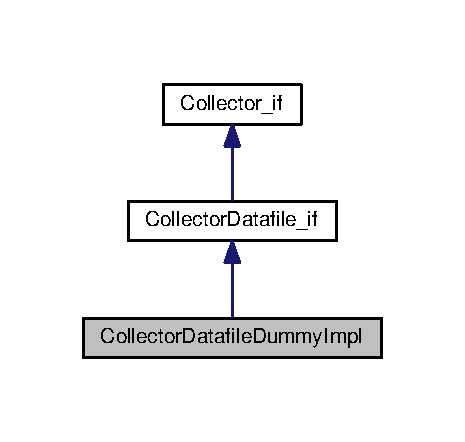
\includegraphics[width=223pt]{class_collector_datafile_dummy_impl__inherit__graph}
\end{center}
\end{figure}


Collaboration diagram for Collector\+Datafile\+Dummy\+Impl\+:\nopagebreak
\begin{figure}[H]
\begin{center}
\leavevmode
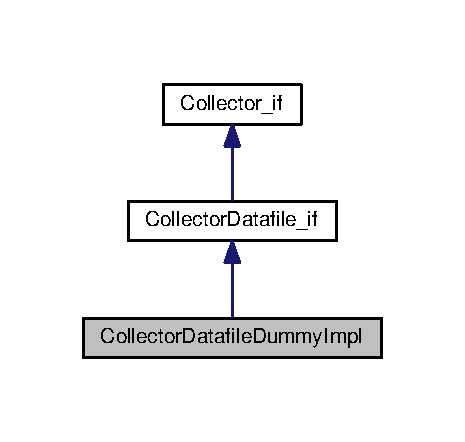
\includegraphics[width=223pt]{class_collector_datafile_dummy_impl__coll__graph}
\end{center}
\end{figure}
\subsection*{Public Member Functions}
\begin{DoxyCompactItemize}
\item 
\hyperlink{class_collector_datafile_dummy_impl_a7ce0478aa682707efd786bea24536d2a}{Collector\+Datafile\+Dummy\+Impl} ()
\item 
\hyperlink{class_collector_datafile_dummy_impl_adfef3c2f2f37459cde3ea8f33030ae49}{Collector\+Datafile\+Dummy\+Impl} (const \hyperlink{class_collector_datafile_dummy_impl}{Collector\+Datafile\+Dummy\+Impl} \&orig)
\item 
\hyperlink{class_collector_datafile_dummy_impl_adafa9e9381c53566ad99fb72ae221f09}{$\sim$\+Collector\+Datafile\+Dummy\+Impl} ()
\item 
void \hyperlink{class_collector_datafile_dummy_impl_a752997589537d0a995da508194fabf7d}{clear} ()
\item 
void \hyperlink{class_collector_datafile_dummy_impl_abf282948e13154ca6a0222508b81c78b}{add\+Value} (double value)
\item 
double \hyperlink{class_collector_datafile_dummy_impl_a8016186fea2815530de9dfa77e9d69ac}{get\+Last\+Value} ()
\item 
unsigned long \hyperlink{class_collector_datafile_dummy_impl_a08cb7f0324844c744b41068ba1bf8d7a}{num\+Elements} ()
\item 
double \hyperlink{class_collector_datafile_dummy_impl_a84eb10b49223b402897c466f93dc1bcf}{get\+Value} (unsigned int num)
\item 
double \hyperlink{class_collector_datafile_dummy_impl_a362d8bf7fee03c319239c994a01cf1ae}{get\+Next\+Value} ()
\item 
void \hyperlink{class_collector_datafile_dummy_impl_a47f415dda26201345746697f700ef1b5}{seek\+First\+Value} ()
\item 
std\+::string \hyperlink{class_collector_datafile_dummy_impl_a33a261f553b05c9c39aa46e1222e4918}{get\+Data\+Filename} ()
\item 
void \hyperlink{class_collector_datafile_dummy_impl_aa2f236e5351f9a438aa7cf8734623758}{set\+Data\+Filename} (std\+::string filename)
\item 
void \hyperlink{class_collector_datafile_dummy_impl_abe4a4a292ae8860d25096bf7184d4a43}{set\+Add\+Value\+Handler} (\hyperlink{_collector__if_8h_ab97c9a368c50eb9e00cb4772e46ff38a}{Collector\+Add\+Value\+Handler} add\+Value\+Handler)
\item 
void \hyperlink{class_collector_datafile_dummy_impl_a1f50e119433718cdd3b3a6b1855e6117}{set\+Clear\+Handler} (\hyperlink{_collector__if_8h_ad22205bb584ed3e0db55fc265a5fe1f4}{Collector\+Clear\+Handler} clear\+Handler)
\end{DoxyCompactItemize}


\subsection{Constructor \& Destructor Documentation}
\index{Collector\+Datafile\+Dummy\+Impl@{Collector\+Datafile\+Dummy\+Impl}!Collector\+Datafile\+Dummy\+Impl@{Collector\+Datafile\+Dummy\+Impl}}
\index{Collector\+Datafile\+Dummy\+Impl@{Collector\+Datafile\+Dummy\+Impl}!Collector\+Datafile\+Dummy\+Impl@{Collector\+Datafile\+Dummy\+Impl}}
\subsubsection[{\texorpdfstring{Collector\+Datafile\+Dummy\+Impl()}{CollectorDatafileDummyImpl()}}]{\setlength{\rightskip}{0pt plus 5cm}Collector\+Datafile\+Dummy\+Impl\+::\+Collector\+Datafile\+Dummy\+Impl (
\begin{DoxyParamCaption}
{}
\end{DoxyParamCaption}
)}\hypertarget{class_collector_datafile_dummy_impl_a7ce0478aa682707efd786bea24536d2a}{}\label{class_collector_datafile_dummy_impl_a7ce0478aa682707efd786bea24536d2a}
\index{Collector\+Datafile\+Dummy\+Impl@{Collector\+Datafile\+Dummy\+Impl}!Collector\+Datafile\+Dummy\+Impl@{Collector\+Datafile\+Dummy\+Impl}}
\index{Collector\+Datafile\+Dummy\+Impl@{Collector\+Datafile\+Dummy\+Impl}!Collector\+Datafile\+Dummy\+Impl@{Collector\+Datafile\+Dummy\+Impl}}
\subsubsection[{\texorpdfstring{Collector\+Datafile\+Dummy\+Impl(const Collector\+Datafile\+Dummy\+Impl \&orig)}{CollectorDatafileDummyImpl(const CollectorDatafileDummyImpl &orig)}}]{\setlength{\rightskip}{0pt plus 5cm}Collector\+Datafile\+Dummy\+Impl\+::\+Collector\+Datafile\+Dummy\+Impl (
\begin{DoxyParamCaption}
\item[{const {\bf Collector\+Datafile\+Dummy\+Impl} \&}]{orig}
\end{DoxyParamCaption}
)}\hypertarget{class_collector_datafile_dummy_impl_adfef3c2f2f37459cde3ea8f33030ae49}{}\label{class_collector_datafile_dummy_impl_adfef3c2f2f37459cde3ea8f33030ae49}
\index{Collector\+Datafile\+Dummy\+Impl@{Collector\+Datafile\+Dummy\+Impl}!````~Collector\+Datafile\+Dummy\+Impl@{$\sim$\+Collector\+Datafile\+Dummy\+Impl}}
\index{````~Collector\+Datafile\+Dummy\+Impl@{$\sim$\+Collector\+Datafile\+Dummy\+Impl}!Collector\+Datafile\+Dummy\+Impl@{Collector\+Datafile\+Dummy\+Impl}}
\subsubsection[{\texorpdfstring{$\sim$\+Collector\+Datafile\+Dummy\+Impl()}{~CollectorDatafileDummyImpl()}}]{\setlength{\rightskip}{0pt plus 5cm}Collector\+Datafile\+Dummy\+Impl\+::$\sim$\+Collector\+Datafile\+Dummy\+Impl (
\begin{DoxyParamCaption}
{}
\end{DoxyParamCaption}
)}\hypertarget{class_collector_datafile_dummy_impl_adafa9e9381c53566ad99fb72ae221f09}{}\label{class_collector_datafile_dummy_impl_adafa9e9381c53566ad99fb72ae221f09}


\subsection{Member Function Documentation}
\index{Collector\+Datafile\+Dummy\+Impl@{Collector\+Datafile\+Dummy\+Impl}!add\+Value@{add\+Value}}
\index{add\+Value@{add\+Value}!Collector\+Datafile\+Dummy\+Impl@{Collector\+Datafile\+Dummy\+Impl}}
\subsubsection[{\texorpdfstring{add\+Value(double value)}{addValue(double value)}}]{\setlength{\rightskip}{0pt plus 5cm}void Collector\+Datafile\+Dummy\+Impl\+::add\+Value (
\begin{DoxyParamCaption}
\item[{double}]{value}
\end{DoxyParamCaption}
)\hspace{0.3cm}{\ttfamily [virtual]}}\hypertarget{class_collector_datafile_dummy_impl_abf282948e13154ca6a0222508b81c78b}{}\label{class_collector_datafile_dummy_impl_abf282948e13154ca6a0222508b81c78b}


Implements \hyperlink{class_collector__if_ac7b83bce8ddb4903d247c1eddd656171}{Collector\+\_\+if}.

\index{Collector\+Datafile\+Dummy\+Impl@{Collector\+Datafile\+Dummy\+Impl}!clear@{clear}}
\index{clear@{clear}!Collector\+Datafile\+Dummy\+Impl@{Collector\+Datafile\+Dummy\+Impl}}
\subsubsection[{\texorpdfstring{clear()}{clear()}}]{\setlength{\rightskip}{0pt plus 5cm}void Collector\+Datafile\+Dummy\+Impl\+::clear (
\begin{DoxyParamCaption}
{}
\end{DoxyParamCaption}
)\hspace{0.3cm}{\ttfamily [virtual]}}\hypertarget{class_collector_datafile_dummy_impl_a752997589537d0a995da508194fabf7d}{}\label{class_collector_datafile_dummy_impl_a752997589537d0a995da508194fabf7d}


Implements \hyperlink{class_collector__if_a035bd1300c85866870c2f6178a9528e8}{Collector\+\_\+if}.

\index{Collector\+Datafile\+Dummy\+Impl@{Collector\+Datafile\+Dummy\+Impl}!get\+Data\+Filename@{get\+Data\+Filename}}
\index{get\+Data\+Filename@{get\+Data\+Filename}!Collector\+Datafile\+Dummy\+Impl@{Collector\+Datafile\+Dummy\+Impl}}
\subsubsection[{\texorpdfstring{get\+Data\+Filename()}{getDataFilename()}}]{\setlength{\rightskip}{0pt plus 5cm}std\+::string Collector\+Datafile\+Dummy\+Impl\+::get\+Data\+Filename (
\begin{DoxyParamCaption}
{}
\end{DoxyParamCaption}
)\hspace{0.3cm}{\ttfamily [virtual]}}\hypertarget{class_collector_datafile_dummy_impl_a33a261f553b05c9c39aa46e1222e4918}{}\label{class_collector_datafile_dummy_impl_a33a261f553b05c9c39aa46e1222e4918}
Get the next value in the file and advances the pointer 

Implements \hyperlink{class_collector_datafile__if_a81d109f34c25f5295f76ba13f4234a3c}{Collector\+Datafile\+\_\+if}.

\index{Collector\+Datafile\+Dummy\+Impl@{Collector\+Datafile\+Dummy\+Impl}!get\+Last\+Value@{get\+Last\+Value}}
\index{get\+Last\+Value@{get\+Last\+Value}!Collector\+Datafile\+Dummy\+Impl@{Collector\+Datafile\+Dummy\+Impl}}
\subsubsection[{\texorpdfstring{get\+Last\+Value()}{getLastValue()}}]{\setlength{\rightskip}{0pt plus 5cm}double Collector\+Datafile\+Dummy\+Impl\+::get\+Last\+Value (
\begin{DoxyParamCaption}
{}
\end{DoxyParamCaption}
)\hspace{0.3cm}{\ttfamily [virtual]}}\hypertarget{class_collector_datafile_dummy_impl_a8016186fea2815530de9dfa77e9d69ac}{}\label{class_collector_datafile_dummy_impl_a8016186fea2815530de9dfa77e9d69ac}


Implements \hyperlink{class_collector__if_aa14f7e1065af8fd38ab592e224fb7e43}{Collector\+\_\+if}.

\index{Collector\+Datafile\+Dummy\+Impl@{Collector\+Datafile\+Dummy\+Impl}!get\+Next\+Value@{get\+Next\+Value}}
\index{get\+Next\+Value@{get\+Next\+Value}!Collector\+Datafile\+Dummy\+Impl@{Collector\+Datafile\+Dummy\+Impl}}
\subsubsection[{\texorpdfstring{get\+Next\+Value()}{getNextValue()}}]{\setlength{\rightskip}{0pt plus 5cm}double Collector\+Datafile\+Dummy\+Impl\+::get\+Next\+Value (
\begin{DoxyParamCaption}
{}
\end{DoxyParamCaption}
)\hspace{0.3cm}{\ttfamily [virtual]}}\hypertarget{class_collector_datafile_dummy_impl_a362d8bf7fee03c319239c994a01cf1ae}{}\label{class_collector_datafile_dummy_impl_a362d8bf7fee03c319239c994a01cf1ae}
Set the pointer to the first value in the file 

Implements \hyperlink{class_collector_datafile__if_a0064b4a740e3590c52ea15790b976dad}{Collector\+Datafile\+\_\+if}.

\index{Collector\+Datafile\+Dummy\+Impl@{Collector\+Datafile\+Dummy\+Impl}!get\+Value@{get\+Value}}
\index{get\+Value@{get\+Value}!Collector\+Datafile\+Dummy\+Impl@{Collector\+Datafile\+Dummy\+Impl}}
\subsubsection[{\texorpdfstring{get\+Value(unsigned int num)}{getValue(unsigned int num)}}]{\setlength{\rightskip}{0pt plus 5cm}double Collector\+Datafile\+Dummy\+Impl\+::get\+Value (
\begin{DoxyParamCaption}
\item[{unsigned int}]{num}
\end{DoxyParamCaption}
)\hspace{0.3cm}{\ttfamily [virtual]}}\hypertarget{class_collector_datafile_dummy_impl_a84eb10b49223b402897c466f93dc1bcf}{}\label{class_collector_datafile_dummy_impl_a84eb10b49223b402897c466f93dc1bcf}


Implements \hyperlink{class_collector_datafile__if_a1f10deeaa49fad2ecf4a4fa4ea262b5c}{Collector\+Datafile\+\_\+if}.

\index{Collector\+Datafile\+Dummy\+Impl@{Collector\+Datafile\+Dummy\+Impl}!num\+Elements@{num\+Elements}}
\index{num\+Elements@{num\+Elements}!Collector\+Datafile\+Dummy\+Impl@{Collector\+Datafile\+Dummy\+Impl}}
\subsubsection[{\texorpdfstring{num\+Elements()}{numElements()}}]{\setlength{\rightskip}{0pt plus 5cm}unsigned long Collector\+Datafile\+Dummy\+Impl\+::num\+Elements (
\begin{DoxyParamCaption}
{}
\end{DoxyParamCaption}
)\hspace{0.3cm}{\ttfamily [virtual]}}\hypertarget{class_collector_datafile_dummy_impl_a08cb7f0324844c744b41068ba1bf8d7a}{}\label{class_collector_datafile_dummy_impl_a08cb7f0324844c744b41068ba1bf8d7a}


Implements \hyperlink{class_collector__if_a97fa632508ffdfad1365b3a949acf745}{Collector\+\_\+if}.

\index{Collector\+Datafile\+Dummy\+Impl@{Collector\+Datafile\+Dummy\+Impl}!seek\+First\+Value@{seek\+First\+Value}}
\index{seek\+First\+Value@{seek\+First\+Value}!Collector\+Datafile\+Dummy\+Impl@{Collector\+Datafile\+Dummy\+Impl}}
\subsubsection[{\texorpdfstring{seek\+First\+Value()}{seekFirstValue()}}]{\setlength{\rightskip}{0pt plus 5cm}void Collector\+Datafile\+Dummy\+Impl\+::seek\+First\+Value (
\begin{DoxyParamCaption}
{}
\end{DoxyParamCaption}
)\hspace{0.3cm}{\ttfamily [virtual]}}\hypertarget{class_collector_datafile_dummy_impl_a47f415dda26201345746697f700ef1b5}{}\label{class_collector_datafile_dummy_impl_a47f415dda26201345746697f700ef1b5}
Get a value from a specific position 

Implements \hyperlink{class_collector_datafile__if_af5d33f603cf60214387a4303adc88969}{Collector\+Datafile\+\_\+if}.

\index{Collector\+Datafile\+Dummy\+Impl@{Collector\+Datafile\+Dummy\+Impl}!set\+Add\+Value\+Handler@{set\+Add\+Value\+Handler}}
\index{set\+Add\+Value\+Handler@{set\+Add\+Value\+Handler}!Collector\+Datafile\+Dummy\+Impl@{Collector\+Datafile\+Dummy\+Impl}}
\subsubsection[{\texorpdfstring{set\+Add\+Value\+Handler(\+Collector\+Add\+Value\+Handler add\+Value\+Handler)}{setAddValueHandler(CollectorAddValueHandler addValueHandler)}}]{\setlength{\rightskip}{0pt plus 5cm}void Collector\+Datafile\+Dummy\+Impl\+::set\+Add\+Value\+Handler (
\begin{DoxyParamCaption}
\item[{{\bf Collector\+Add\+Value\+Handler}}]{add\+Value\+Handler}
\end{DoxyParamCaption}
)\hspace{0.3cm}{\ttfamily [virtual]}}\hypertarget{class_collector_datafile_dummy_impl_abe4a4a292ae8860d25096bf7184d4a43}{}\label{class_collector_datafile_dummy_impl_abe4a4a292ae8860d25096bf7184d4a43}


Implements \hyperlink{class_collector__if_a71e66a9bb8a91832ec7a05a1fe00519e}{Collector\+\_\+if}.

\index{Collector\+Datafile\+Dummy\+Impl@{Collector\+Datafile\+Dummy\+Impl}!set\+Clear\+Handler@{set\+Clear\+Handler}}
\index{set\+Clear\+Handler@{set\+Clear\+Handler}!Collector\+Datafile\+Dummy\+Impl@{Collector\+Datafile\+Dummy\+Impl}}
\subsubsection[{\texorpdfstring{set\+Clear\+Handler(\+Collector\+Clear\+Handler clear\+Handler)}{setClearHandler(CollectorClearHandler clearHandler)}}]{\setlength{\rightskip}{0pt plus 5cm}void Collector\+Datafile\+Dummy\+Impl\+::set\+Clear\+Handler (
\begin{DoxyParamCaption}
\item[{{\bf Collector\+Clear\+Handler}}]{clear\+Handler}
\end{DoxyParamCaption}
)\hspace{0.3cm}{\ttfamily [virtual]}}\hypertarget{class_collector_datafile_dummy_impl_a1f50e119433718cdd3b3a6b1855e6117}{}\label{class_collector_datafile_dummy_impl_a1f50e119433718cdd3b3a6b1855e6117}


Implements \hyperlink{class_collector__if_ac03e3c41ccfe3aff6f6a0b3aca8c885b}{Collector\+\_\+if}.

\index{Collector\+Datafile\+Dummy\+Impl@{Collector\+Datafile\+Dummy\+Impl}!set\+Data\+Filename@{set\+Data\+Filename}}
\index{set\+Data\+Filename@{set\+Data\+Filename}!Collector\+Datafile\+Dummy\+Impl@{Collector\+Datafile\+Dummy\+Impl}}
\subsubsection[{\texorpdfstring{set\+Data\+Filename(std\+::string filename)}{setDataFilename(std::string filename)}}]{\setlength{\rightskip}{0pt plus 5cm}void Collector\+Datafile\+Dummy\+Impl\+::set\+Data\+Filename (
\begin{DoxyParamCaption}
\item[{std\+::string}]{filename}
\end{DoxyParamCaption}
)\hspace{0.3cm}{\ttfamily [virtual]}}\hypertarget{class_collector_datafile_dummy_impl_aa2f236e5351f9a438aa7cf8734623758}{}\label{class_collector_datafile_dummy_impl_aa2f236e5351f9a438aa7cf8734623758}


Implements \hyperlink{class_collector_datafile__if_ab826bbf5472a5cfdbf2f2c30273da8eb}{Collector\+Datafile\+\_\+if}.



The documentation for this class was generated from the following files\+:\begin{DoxyCompactItemize}
\item 
\hyperlink{_collector_datafile_dummy_impl_8h}{Collector\+Datafile\+Dummy\+Impl.\+h}\item 
\hyperlink{_collector_datafile_dummy_impl_8cpp}{Collector\+Datafile\+Dummy\+Impl.\+cpp}\end{DoxyCompactItemize}

\hypertarget{class_collector_default_impl1}{}\section{Collector\+Default\+Impl1 Class Reference}
\label{class_collector_default_impl1}\index{Collector\+Default\+Impl1@{Collector\+Default\+Impl1}}


{\ttfamily \#include $<$Collector\+Default\+Impl1.\+h$>$}



Inheritance diagram for Collector\+Default\+Impl1\+:\nopagebreak
\begin{figure}[H]
\begin{center}
\leavevmode
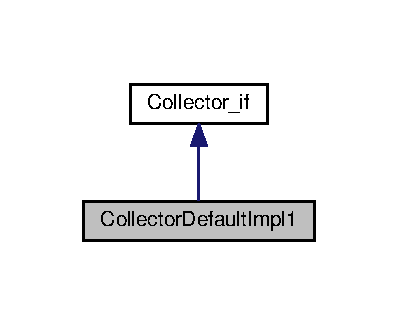
\includegraphics[width=191pt]{class_collector_default_impl1__inherit__graph}
\end{center}
\end{figure}


Collaboration diagram for Collector\+Default\+Impl1\+:\nopagebreak
\begin{figure}[H]
\begin{center}
\leavevmode
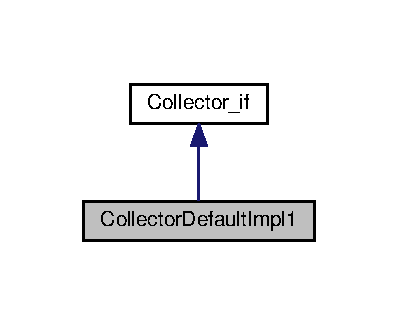
\includegraphics[width=191pt]{class_collector_default_impl1__coll__graph}
\end{center}
\end{figure}
\subsection*{Public Member Functions}
\begin{DoxyCompactItemize}
\item 
\hyperlink{class_collector_default_impl1_a6bfa3d5ce8f4603b8045d4ffe8b230fb}{Collector\+Default\+Impl1} ()
\item 
\hyperlink{class_collector_default_impl1_aa112499b149d7402d5f070c3ad444936}{Collector\+Default\+Impl1} (const \hyperlink{class_collector_default_impl1}{Collector\+Default\+Impl1} \&orig)
\item 
virtual \hyperlink{class_collector_default_impl1_a09fb71c2c989c7c4b13188c8ede239f3}{$\sim$\+Collector\+Default\+Impl1} ()
\item 
void \hyperlink{class_collector_default_impl1_a82eb6c21e7810cf904710e7652559358}{clear} ()
\item 
void \hyperlink{class_collector_default_impl1_a2e36071e83b5b3f92633dbd1e5dcb127}{add\+Value} (double value)
\item 
double \hyperlink{class_collector_default_impl1_a13bb1928b87505141d730b348cc9b7ea}{get\+Last\+Value} ()
\item 
unsigned long \hyperlink{class_collector_default_impl1_a29ac5b9cca189d1fc18064374a378b85}{num\+Elements} ()
\item 
void \hyperlink{class_collector_default_impl1_ab6967cf9fdf439953cc3dd10e711fc7d}{set\+Add\+Value\+Handler} (\hyperlink{_collector__if_8h_ab97c9a368c50eb9e00cb4772e46ff38a}{Collector\+Add\+Value\+Handler} add\+Value\+Handler)
\item 
void \hyperlink{class_collector_default_impl1_a2b64c9abd7acea19fe57eb2d6a18ea9f}{set\+Clear\+Handler} (\hyperlink{_collector__if_8h_ad22205bb584ed3e0db55fc265a5fe1f4}{Collector\+Clear\+Handler} clear\+Handler)
\end{DoxyCompactItemize}


\subsection{Constructor \& Destructor Documentation}
\index{Collector\+Default\+Impl1@{Collector\+Default\+Impl1}!Collector\+Default\+Impl1@{Collector\+Default\+Impl1}}
\index{Collector\+Default\+Impl1@{Collector\+Default\+Impl1}!Collector\+Default\+Impl1@{Collector\+Default\+Impl1}}
\subsubsection[{\texorpdfstring{Collector\+Default\+Impl1()}{CollectorDefaultImpl1()}}]{\setlength{\rightskip}{0pt plus 5cm}Collector\+Default\+Impl1\+::\+Collector\+Default\+Impl1 (
\begin{DoxyParamCaption}
{}
\end{DoxyParamCaption}
)}\hypertarget{class_collector_default_impl1_a6bfa3d5ce8f4603b8045d4ffe8b230fb}{}\label{class_collector_default_impl1_a6bfa3d5ce8f4603b8045d4ffe8b230fb}
\index{Collector\+Default\+Impl1@{Collector\+Default\+Impl1}!Collector\+Default\+Impl1@{Collector\+Default\+Impl1}}
\index{Collector\+Default\+Impl1@{Collector\+Default\+Impl1}!Collector\+Default\+Impl1@{Collector\+Default\+Impl1}}
\subsubsection[{\texorpdfstring{Collector\+Default\+Impl1(const Collector\+Default\+Impl1 \&orig)}{CollectorDefaultImpl1(const CollectorDefaultImpl1 &orig)}}]{\setlength{\rightskip}{0pt plus 5cm}Collector\+Default\+Impl1\+::\+Collector\+Default\+Impl1 (
\begin{DoxyParamCaption}
\item[{const {\bf Collector\+Default\+Impl1} \&}]{orig}
\end{DoxyParamCaption}
)}\hypertarget{class_collector_default_impl1_aa112499b149d7402d5f070c3ad444936}{}\label{class_collector_default_impl1_aa112499b149d7402d5f070c3ad444936}
\index{Collector\+Default\+Impl1@{Collector\+Default\+Impl1}!````~Collector\+Default\+Impl1@{$\sim$\+Collector\+Default\+Impl1}}
\index{````~Collector\+Default\+Impl1@{$\sim$\+Collector\+Default\+Impl1}!Collector\+Default\+Impl1@{Collector\+Default\+Impl1}}
\subsubsection[{\texorpdfstring{$\sim$\+Collector\+Default\+Impl1()}{~CollectorDefaultImpl1()}}]{\setlength{\rightskip}{0pt plus 5cm}Collector\+Default\+Impl1\+::$\sim$\+Collector\+Default\+Impl1 (
\begin{DoxyParamCaption}
{}
\end{DoxyParamCaption}
)\hspace{0.3cm}{\ttfamily [virtual]}}\hypertarget{class_collector_default_impl1_a09fb71c2c989c7c4b13188c8ede239f3}{}\label{class_collector_default_impl1_a09fb71c2c989c7c4b13188c8ede239f3}


\subsection{Member Function Documentation}
\index{Collector\+Default\+Impl1@{Collector\+Default\+Impl1}!add\+Value@{add\+Value}}
\index{add\+Value@{add\+Value}!Collector\+Default\+Impl1@{Collector\+Default\+Impl1}}
\subsubsection[{\texorpdfstring{add\+Value(double value)}{addValue(double value)}}]{\setlength{\rightskip}{0pt plus 5cm}void Collector\+Default\+Impl1\+::add\+Value (
\begin{DoxyParamCaption}
\item[{double}]{value}
\end{DoxyParamCaption}
)\hspace{0.3cm}{\ttfamily [virtual]}}\hypertarget{class_collector_default_impl1_a2e36071e83b5b3f92633dbd1e5dcb127}{}\label{class_collector_default_impl1_a2e36071e83b5b3f92633dbd1e5dcb127}


Implements \hyperlink{class_collector__if_ac7b83bce8ddb4903d247c1eddd656171}{Collector\+\_\+if}.

\index{Collector\+Default\+Impl1@{Collector\+Default\+Impl1}!clear@{clear}}
\index{clear@{clear}!Collector\+Default\+Impl1@{Collector\+Default\+Impl1}}
\subsubsection[{\texorpdfstring{clear()}{clear()}}]{\setlength{\rightskip}{0pt plus 5cm}void Collector\+Default\+Impl1\+::clear (
\begin{DoxyParamCaption}
{}
\end{DoxyParamCaption}
)\hspace{0.3cm}{\ttfamily [virtual]}}\hypertarget{class_collector_default_impl1_a82eb6c21e7810cf904710e7652559358}{}\label{class_collector_default_impl1_a82eb6c21e7810cf904710e7652559358}


Implements \hyperlink{class_collector__if_a035bd1300c85866870c2f6178a9528e8}{Collector\+\_\+if}.

\index{Collector\+Default\+Impl1@{Collector\+Default\+Impl1}!get\+Last\+Value@{get\+Last\+Value}}
\index{get\+Last\+Value@{get\+Last\+Value}!Collector\+Default\+Impl1@{Collector\+Default\+Impl1}}
\subsubsection[{\texorpdfstring{get\+Last\+Value()}{getLastValue()}}]{\setlength{\rightskip}{0pt plus 5cm}double Collector\+Default\+Impl1\+::get\+Last\+Value (
\begin{DoxyParamCaption}
{}
\end{DoxyParamCaption}
)\hspace{0.3cm}{\ttfamily [virtual]}}\hypertarget{class_collector_default_impl1_a13bb1928b87505141d730b348cc9b7ea}{}\label{class_collector_default_impl1_a13bb1928b87505141d730b348cc9b7ea}


Implements \hyperlink{class_collector__if_aa14f7e1065af8fd38ab592e224fb7e43}{Collector\+\_\+if}.

\index{Collector\+Default\+Impl1@{Collector\+Default\+Impl1}!num\+Elements@{num\+Elements}}
\index{num\+Elements@{num\+Elements}!Collector\+Default\+Impl1@{Collector\+Default\+Impl1}}
\subsubsection[{\texorpdfstring{num\+Elements()}{numElements()}}]{\setlength{\rightskip}{0pt plus 5cm}unsigned long Collector\+Default\+Impl1\+::num\+Elements (
\begin{DoxyParamCaption}
{}
\end{DoxyParamCaption}
)\hspace{0.3cm}{\ttfamily [virtual]}}\hypertarget{class_collector_default_impl1_a29ac5b9cca189d1fc18064374a378b85}{}\label{class_collector_default_impl1_a29ac5b9cca189d1fc18064374a378b85}


Implements \hyperlink{class_collector__if_a97fa632508ffdfad1365b3a949acf745}{Collector\+\_\+if}.

\index{Collector\+Default\+Impl1@{Collector\+Default\+Impl1}!set\+Add\+Value\+Handler@{set\+Add\+Value\+Handler}}
\index{set\+Add\+Value\+Handler@{set\+Add\+Value\+Handler}!Collector\+Default\+Impl1@{Collector\+Default\+Impl1}}
\subsubsection[{\texorpdfstring{set\+Add\+Value\+Handler(\+Collector\+Add\+Value\+Handler add\+Value\+Handler)}{setAddValueHandler(CollectorAddValueHandler addValueHandler)}}]{\setlength{\rightskip}{0pt plus 5cm}void Collector\+Default\+Impl1\+::set\+Add\+Value\+Handler (
\begin{DoxyParamCaption}
\item[{{\bf Collector\+Add\+Value\+Handler}}]{add\+Value\+Handler}
\end{DoxyParamCaption}
)\hspace{0.3cm}{\ttfamily [virtual]}}\hypertarget{class_collector_default_impl1_ab6967cf9fdf439953cc3dd10e711fc7d}{}\label{class_collector_default_impl1_ab6967cf9fdf439953cc3dd10e711fc7d}


Implements \hyperlink{class_collector__if_a71e66a9bb8a91832ec7a05a1fe00519e}{Collector\+\_\+if}.

\index{Collector\+Default\+Impl1@{Collector\+Default\+Impl1}!set\+Clear\+Handler@{set\+Clear\+Handler}}
\index{set\+Clear\+Handler@{set\+Clear\+Handler}!Collector\+Default\+Impl1@{Collector\+Default\+Impl1}}
\subsubsection[{\texorpdfstring{set\+Clear\+Handler(\+Collector\+Clear\+Handler clear\+Handler)}{setClearHandler(CollectorClearHandler clearHandler)}}]{\setlength{\rightskip}{0pt plus 5cm}void Collector\+Default\+Impl1\+::set\+Clear\+Handler (
\begin{DoxyParamCaption}
\item[{{\bf Collector\+Clear\+Handler}}]{clear\+Handler}
\end{DoxyParamCaption}
)\hspace{0.3cm}{\ttfamily [virtual]}}\hypertarget{class_collector_default_impl1_a2b64c9abd7acea19fe57eb2d6a18ea9f}{}\label{class_collector_default_impl1_a2b64c9abd7acea19fe57eb2d6a18ea9f}


Implements \hyperlink{class_collector__if_ac03e3c41ccfe3aff6f6a0b3aca8c885b}{Collector\+\_\+if}.



The documentation for this class was generated from the following files\+:\begin{DoxyCompactItemize}
\item 
\hyperlink{_collector_default_impl1_8h}{Collector\+Default\+Impl1.\+h}\item 
\hyperlink{_collector_default_impl1_8cpp}{Collector\+Default\+Impl1.\+cpp}\end{DoxyCompactItemize}

\hypertarget{class_collector_dummy_impl}{}\section{Collector\+Dummy\+Impl Class Reference}
\label{class_collector_dummy_impl}\index{Collector\+Dummy\+Impl@{Collector\+Dummy\+Impl}}


{\ttfamily \#include $<$Collector\+Dummy\+Impl.\+h$>$}



Inheritance diagram for Collector\+Dummy\+Impl\+:
\nopagebreak
\begin{figure}[H]
\begin{center}
\leavevmode
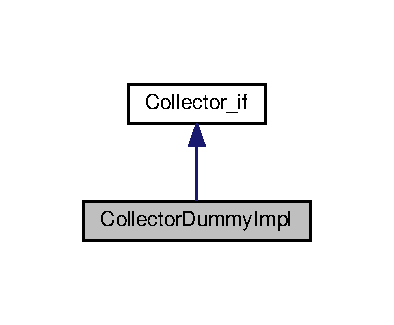
\includegraphics[width=189pt]{class_collector_dummy_impl__inherit__graph}
\end{center}
\end{figure}


Collaboration diagram for Collector\+Dummy\+Impl\+:
\nopagebreak
\begin{figure}[H]
\begin{center}
\leavevmode
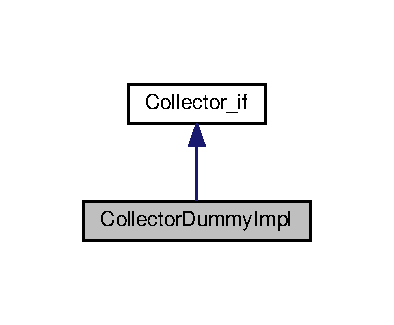
\includegraphics[width=189pt]{class_collector_dummy_impl__coll__graph}
\end{center}
\end{figure}
\subsection*{Public Member Functions}
\begin{DoxyCompactItemize}
\item 
\hyperlink{class_collector_dummy_impl_a68bb20ef5365fa245738a77a5a6775a3}{Collector\+Dummy\+Impl} ()
\item 
\hyperlink{class_collector_dummy_impl_a79e4c4e9c26f55329185b51effbcaeba}{Collector\+Dummy\+Impl} (const \hyperlink{class_collector_dummy_impl}{Collector\+Dummy\+Impl} \&orig)
\item 
\hyperlink{class_collector_dummy_impl_a7b67a55b121dab990b2b8bbf3dd4bdb5}{$\sim$\+Collector\+Dummy\+Impl} ()
\item 
void \hyperlink{class_collector_dummy_impl_ae46c9c7311ee0ed2cc5fb1a3489efa77}{clear} ()
\item 
void \hyperlink{class_collector_dummy_impl_a1844cfacaf10eb42bd6f370592246223}{add\+Value} (double value)
\item 
double \hyperlink{class_collector_dummy_impl_af19161da4eb1332b1f20b3fd6e96bd85}{get\+Last\+Value} ()
\item 
unsigned long \hyperlink{class_collector_dummy_impl_a92241b24f8a0017c355879a204f94266}{num\+Elements} ()
\end{DoxyCompactItemize}


\subsection{Constructor \& Destructor Documentation}
\index{Collector\+Dummy\+Impl@{Collector\+Dummy\+Impl}!Collector\+Dummy\+Impl@{Collector\+Dummy\+Impl}}
\index{Collector\+Dummy\+Impl@{Collector\+Dummy\+Impl}!Collector\+Dummy\+Impl@{Collector\+Dummy\+Impl}}
\subsubsection[{\texorpdfstring{Collector\+Dummy\+Impl()}{CollectorDummyImpl()}}]{\setlength{\rightskip}{0pt plus 5cm}Collector\+Dummy\+Impl\+::\+Collector\+Dummy\+Impl (
\begin{DoxyParamCaption}
{}
\end{DoxyParamCaption}
)}\hypertarget{class_collector_dummy_impl_a68bb20ef5365fa245738a77a5a6775a3}{}\label{class_collector_dummy_impl_a68bb20ef5365fa245738a77a5a6775a3}
\index{Collector\+Dummy\+Impl@{Collector\+Dummy\+Impl}!Collector\+Dummy\+Impl@{Collector\+Dummy\+Impl}}
\index{Collector\+Dummy\+Impl@{Collector\+Dummy\+Impl}!Collector\+Dummy\+Impl@{Collector\+Dummy\+Impl}}
\subsubsection[{\texorpdfstring{Collector\+Dummy\+Impl(const Collector\+Dummy\+Impl \&orig)}{CollectorDummyImpl(const CollectorDummyImpl &orig)}}]{\setlength{\rightskip}{0pt plus 5cm}Collector\+Dummy\+Impl\+::\+Collector\+Dummy\+Impl (
\begin{DoxyParamCaption}
\item[{const {\bf Collector\+Dummy\+Impl} \&}]{orig}
\end{DoxyParamCaption}
)}\hypertarget{class_collector_dummy_impl_a79e4c4e9c26f55329185b51effbcaeba}{}\label{class_collector_dummy_impl_a79e4c4e9c26f55329185b51effbcaeba}
\index{Collector\+Dummy\+Impl@{Collector\+Dummy\+Impl}!````~Collector\+Dummy\+Impl@{$\sim$\+Collector\+Dummy\+Impl}}
\index{````~Collector\+Dummy\+Impl@{$\sim$\+Collector\+Dummy\+Impl}!Collector\+Dummy\+Impl@{Collector\+Dummy\+Impl}}
\subsubsection[{\texorpdfstring{$\sim$\+Collector\+Dummy\+Impl()}{~CollectorDummyImpl()}}]{\setlength{\rightskip}{0pt plus 5cm}Collector\+Dummy\+Impl\+::$\sim$\+Collector\+Dummy\+Impl (
\begin{DoxyParamCaption}
{}
\end{DoxyParamCaption}
)}\hypertarget{class_collector_dummy_impl_a7b67a55b121dab990b2b8bbf3dd4bdb5}{}\label{class_collector_dummy_impl_a7b67a55b121dab990b2b8bbf3dd4bdb5}


\subsection{Member Function Documentation}
\index{Collector\+Dummy\+Impl@{Collector\+Dummy\+Impl}!add\+Value@{add\+Value}}
\index{add\+Value@{add\+Value}!Collector\+Dummy\+Impl@{Collector\+Dummy\+Impl}}
\subsubsection[{\texorpdfstring{add\+Value(double value)}{addValue(double value)}}]{\setlength{\rightskip}{0pt plus 5cm}void Collector\+Dummy\+Impl\+::add\+Value (
\begin{DoxyParamCaption}
\item[{double}]{value}
\end{DoxyParamCaption}
)\hspace{0.3cm}{\ttfamily [virtual]}}\hypertarget{class_collector_dummy_impl_a1844cfacaf10eb42bd6f370592246223}{}\label{class_collector_dummy_impl_a1844cfacaf10eb42bd6f370592246223}


Implements \hyperlink{class_collector__if_ac7b83bce8ddb4903d247c1eddd656171}{Collector\+\_\+if}.

\index{Collector\+Dummy\+Impl@{Collector\+Dummy\+Impl}!clear@{clear}}
\index{clear@{clear}!Collector\+Dummy\+Impl@{Collector\+Dummy\+Impl}}
\subsubsection[{\texorpdfstring{clear()}{clear()}}]{\setlength{\rightskip}{0pt plus 5cm}void Collector\+Dummy\+Impl\+::clear (
\begin{DoxyParamCaption}
{}
\end{DoxyParamCaption}
)\hspace{0.3cm}{\ttfamily [virtual]}}\hypertarget{class_collector_dummy_impl_ae46c9c7311ee0ed2cc5fb1a3489efa77}{}\label{class_collector_dummy_impl_ae46c9c7311ee0ed2cc5fb1a3489efa77}


Implements \hyperlink{class_collector__if_a035bd1300c85866870c2f6178a9528e8}{Collector\+\_\+if}.

\index{Collector\+Dummy\+Impl@{Collector\+Dummy\+Impl}!get\+Last\+Value@{get\+Last\+Value}}
\index{get\+Last\+Value@{get\+Last\+Value}!Collector\+Dummy\+Impl@{Collector\+Dummy\+Impl}}
\subsubsection[{\texorpdfstring{get\+Last\+Value()}{getLastValue()}}]{\setlength{\rightskip}{0pt plus 5cm}double Collector\+Dummy\+Impl\+::get\+Last\+Value (
\begin{DoxyParamCaption}
{}
\end{DoxyParamCaption}
)\hspace{0.3cm}{\ttfamily [virtual]}}\hypertarget{class_collector_dummy_impl_af19161da4eb1332b1f20b3fd6e96bd85}{}\label{class_collector_dummy_impl_af19161da4eb1332b1f20b3fd6e96bd85}


Implements \hyperlink{class_collector__if_aa14f7e1065af8fd38ab592e224fb7e43}{Collector\+\_\+if}.

\index{Collector\+Dummy\+Impl@{Collector\+Dummy\+Impl}!num\+Elements@{num\+Elements}}
\index{num\+Elements@{num\+Elements}!Collector\+Dummy\+Impl@{Collector\+Dummy\+Impl}}
\subsubsection[{\texorpdfstring{num\+Elements()}{numElements()}}]{\setlength{\rightskip}{0pt plus 5cm}unsigned long Collector\+Dummy\+Impl\+::num\+Elements (
\begin{DoxyParamCaption}
{}
\end{DoxyParamCaption}
)\hspace{0.3cm}{\ttfamily [virtual]}}\hypertarget{class_collector_dummy_impl_a92241b24f8a0017c355879a204f94266}{}\label{class_collector_dummy_impl_a92241b24f8a0017c355879a204f94266}


Implements \hyperlink{class_collector__if_a97fa632508ffdfad1365b3a949acf745}{Collector\+\_\+if}.



The documentation for this class was generated from the following files\+:\begin{DoxyCompactItemize}
\item 
\hyperlink{_collector_dummy_impl_8h}{Collector\+Dummy\+Impl.\+h}\item 
\hyperlink{_collector_dummy_impl_8cpp}{Collector\+Dummy\+Impl.\+cpp}\end{DoxyCompactItemize}

\hypertarget{class_create}{}\section{Create Class Reference}
\label{class_create}\index{Create@{Create}}


{\ttfamily \#include $<$Create.\+h$>$}



Inheritance diagram for Create\+:\nopagebreak
\begin{figure}[H]
\begin{center}
\leavevmode
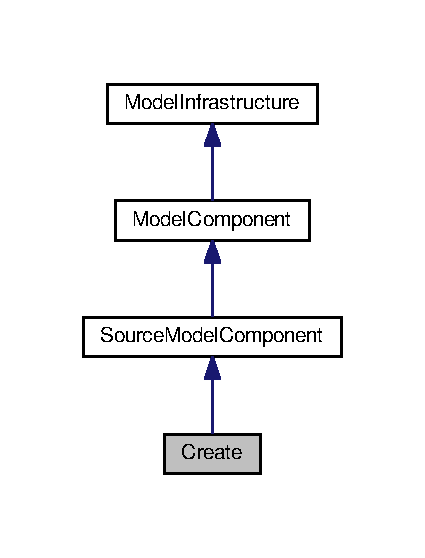
\includegraphics[width=204pt]{class_create__inherit__graph}
\end{center}
\end{figure}


Collaboration diagram for Create\+:\nopagebreak
\begin{figure}[H]
\begin{center}
\leavevmode
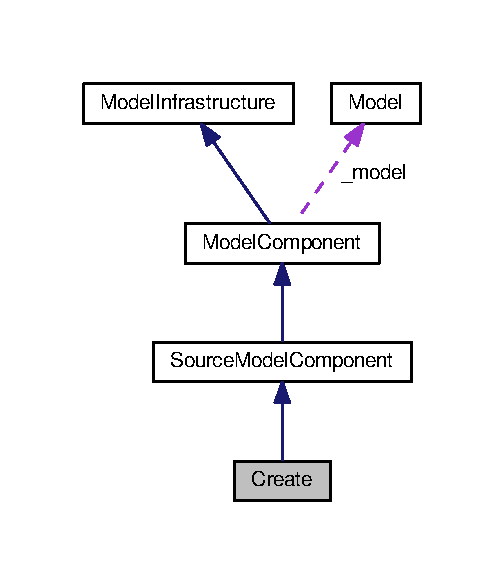
\includegraphics[width=256pt]{class_create__coll__graph}
\end{center}
\end{figure}
\subsection*{Public Member Functions}
\begin{DoxyCompactItemize}
\item 
\hyperlink{class_create_a81bd7a50b926660c264ebe29e2095170}{Create} (\hyperlink{class_model}{Model} $\ast$model)
\item 
\hyperlink{class_create_a035a6f7ddd02dace181b23913b91bad9}{Create} (const \hyperlink{class_create}{Create} \&orig)
\item 
virtual \hyperlink{class_create_a6060fda2b105228446ddddb09f63d127}{$\sim$\+Create} ()
\item 
virtual std\+::string \hyperlink{class_create_a8d1832d2165bbeea4a5a88aded883f86}{show} ()
\end{DoxyCompactItemize}
\subsection*{Protected Member Functions}
\begin{DoxyCompactItemize}
\item 
virtual void \hyperlink{class_create_acd3a4b8805561591e0c88d3fd689cf74}{\+\_\+execute} (\hyperlink{class_entity}{Entity} $\ast$entity)
\item 
virtual void \hyperlink{class_create_aaa3cb1a4359586b0b8df817f57916286}{\+\_\+load\+Instance} (std\+::list$<$ std\+::string $>$ words)
\item 
virtual std\+::list$<$ std\+::string $>$ $\ast$ \hyperlink{class_create_ae1fd0c281cec35dcf91881acba8d7041}{\+\_\+save\+Instance} ()
\item 
virtual bool \hyperlink{class_create_ad445fd3bec94b4e66669089f10f96057}{\+\_\+verify\+Symbols} (std\+::string $\ast$error\+Message)
\end{DoxyCompactItemize}
\subsection*{Additional Inherited Members}


\subsection{Detailed Description}
\hyperlink{class_create}{Create} is the most basic component to include the first entities into the model, and therefore is a source component (derived from \hyperlink{class_source_model_component}{Source\+Model\+Component}) 

\subsection{Constructor \& Destructor Documentation}
\index{Create@{Create}!Create@{Create}}
\index{Create@{Create}!Create@{Create}}
\subsubsection[{\texorpdfstring{Create(\+Model $\ast$model)}{Create(Model *model)}}]{\setlength{\rightskip}{0pt plus 5cm}Create\+::\+Create (
\begin{DoxyParamCaption}
\item[{{\bf Model} $\ast$}]{model}
\end{DoxyParamCaption}
)}\hypertarget{class_create_a81bd7a50b926660c264ebe29e2095170}{}\label{class_create_a81bd7a50b926660c264ebe29e2095170}


Here is the call graph for this function\+:\nopagebreak
\begin{figure}[H]
\begin{center}
\leavevmode
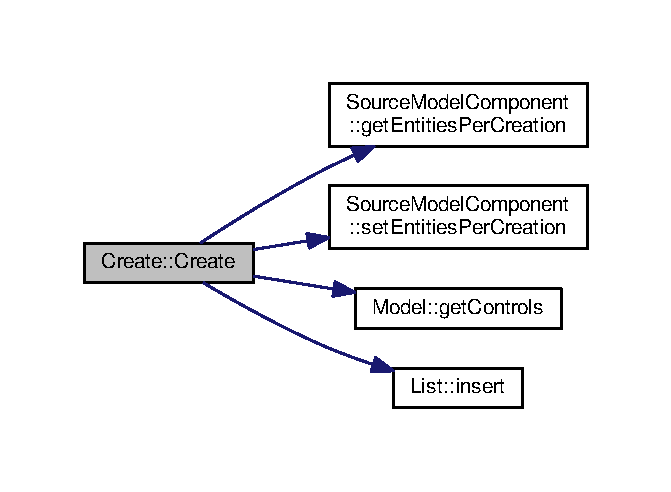
\includegraphics[width=321pt]{class_create_a81bd7a50b926660c264ebe29e2095170_cgraph}
\end{center}
\end{figure}


\index{Create@{Create}!Create@{Create}}
\index{Create@{Create}!Create@{Create}}
\subsubsection[{\texorpdfstring{Create(const Create \&orig)}{Create(const Create &orig)}}]{\setlength{\rightskip}{0pt plus 5cm}Create\+::\+Create (
\begin{DoxyParamCaption}
\item[{const {\bf Create} \&}]{orig}
\end{DoxyParamCaption}
)}\hypertarget{class_create_a035a6f7ddd02dace181b23913b91bad9}{}\label{class_create_a035a6f7ddd02dace181b23913b91bad9}
\index{Create@{Create}!````~Create@{$\sim$\+Create}}
\index{````~Create@{$\sim$\+Create}!Create@{Create}}
\subsubsection[{\texorpdfstring{$\sim$\+Create()}{~Create()}}]{\setlength{\rightskip}{0pt plus 5cm}Create\+::$\sim$\+Create (
\begin{DoxyParamCaption}
{}
\end{DoxyParamCaption}
)\hspace{0.3cm}{\ttfamily [virtual]}}\hypertarget{class_create_a6060fda2b105228446ddddb09f63d127}{}\label{class_create_a6060fda2b105228446ddddb09f63d127}


\subsection{Member Function Documentation}
\index{Create@{Create}!\+\_\+execute@{\+\_\+execute}}
\index{\+\_\+execute@{\+\_\+execute}!Create@{Create}}
\subsubsection[{\texorpdfstring{\+\_\+execute(\+Entity $\ast$entity)}{_execute(Entity *entity)}}]{\setlength{\rightskip}{0pt plus 5cm}void Create\+::\+\_\+execute (
\begin{DoxyParamCaption}
\item[{{\bf Entity} $\ast$}]{entity}
\end{DoxyParamCaption}
)\hspace{0.3cm}{\ttfamily [protected]}, {\ttfamily [virtual]}}\hypertarget{class_create_acd3a4b8805561591e0c88d3fd689cf74}{}\label{class_create_acd3a4b8805561591e0c88d3fd689cf74}


Implements \hyperlink{class_model_component_ae3fcf8bbdd8368c882438424aa73f714}{Model\+Component}.



Here is the call graph for this function\+:\nopagebreak
\begin{figure}[H]
\begin{center}
\leavevmode
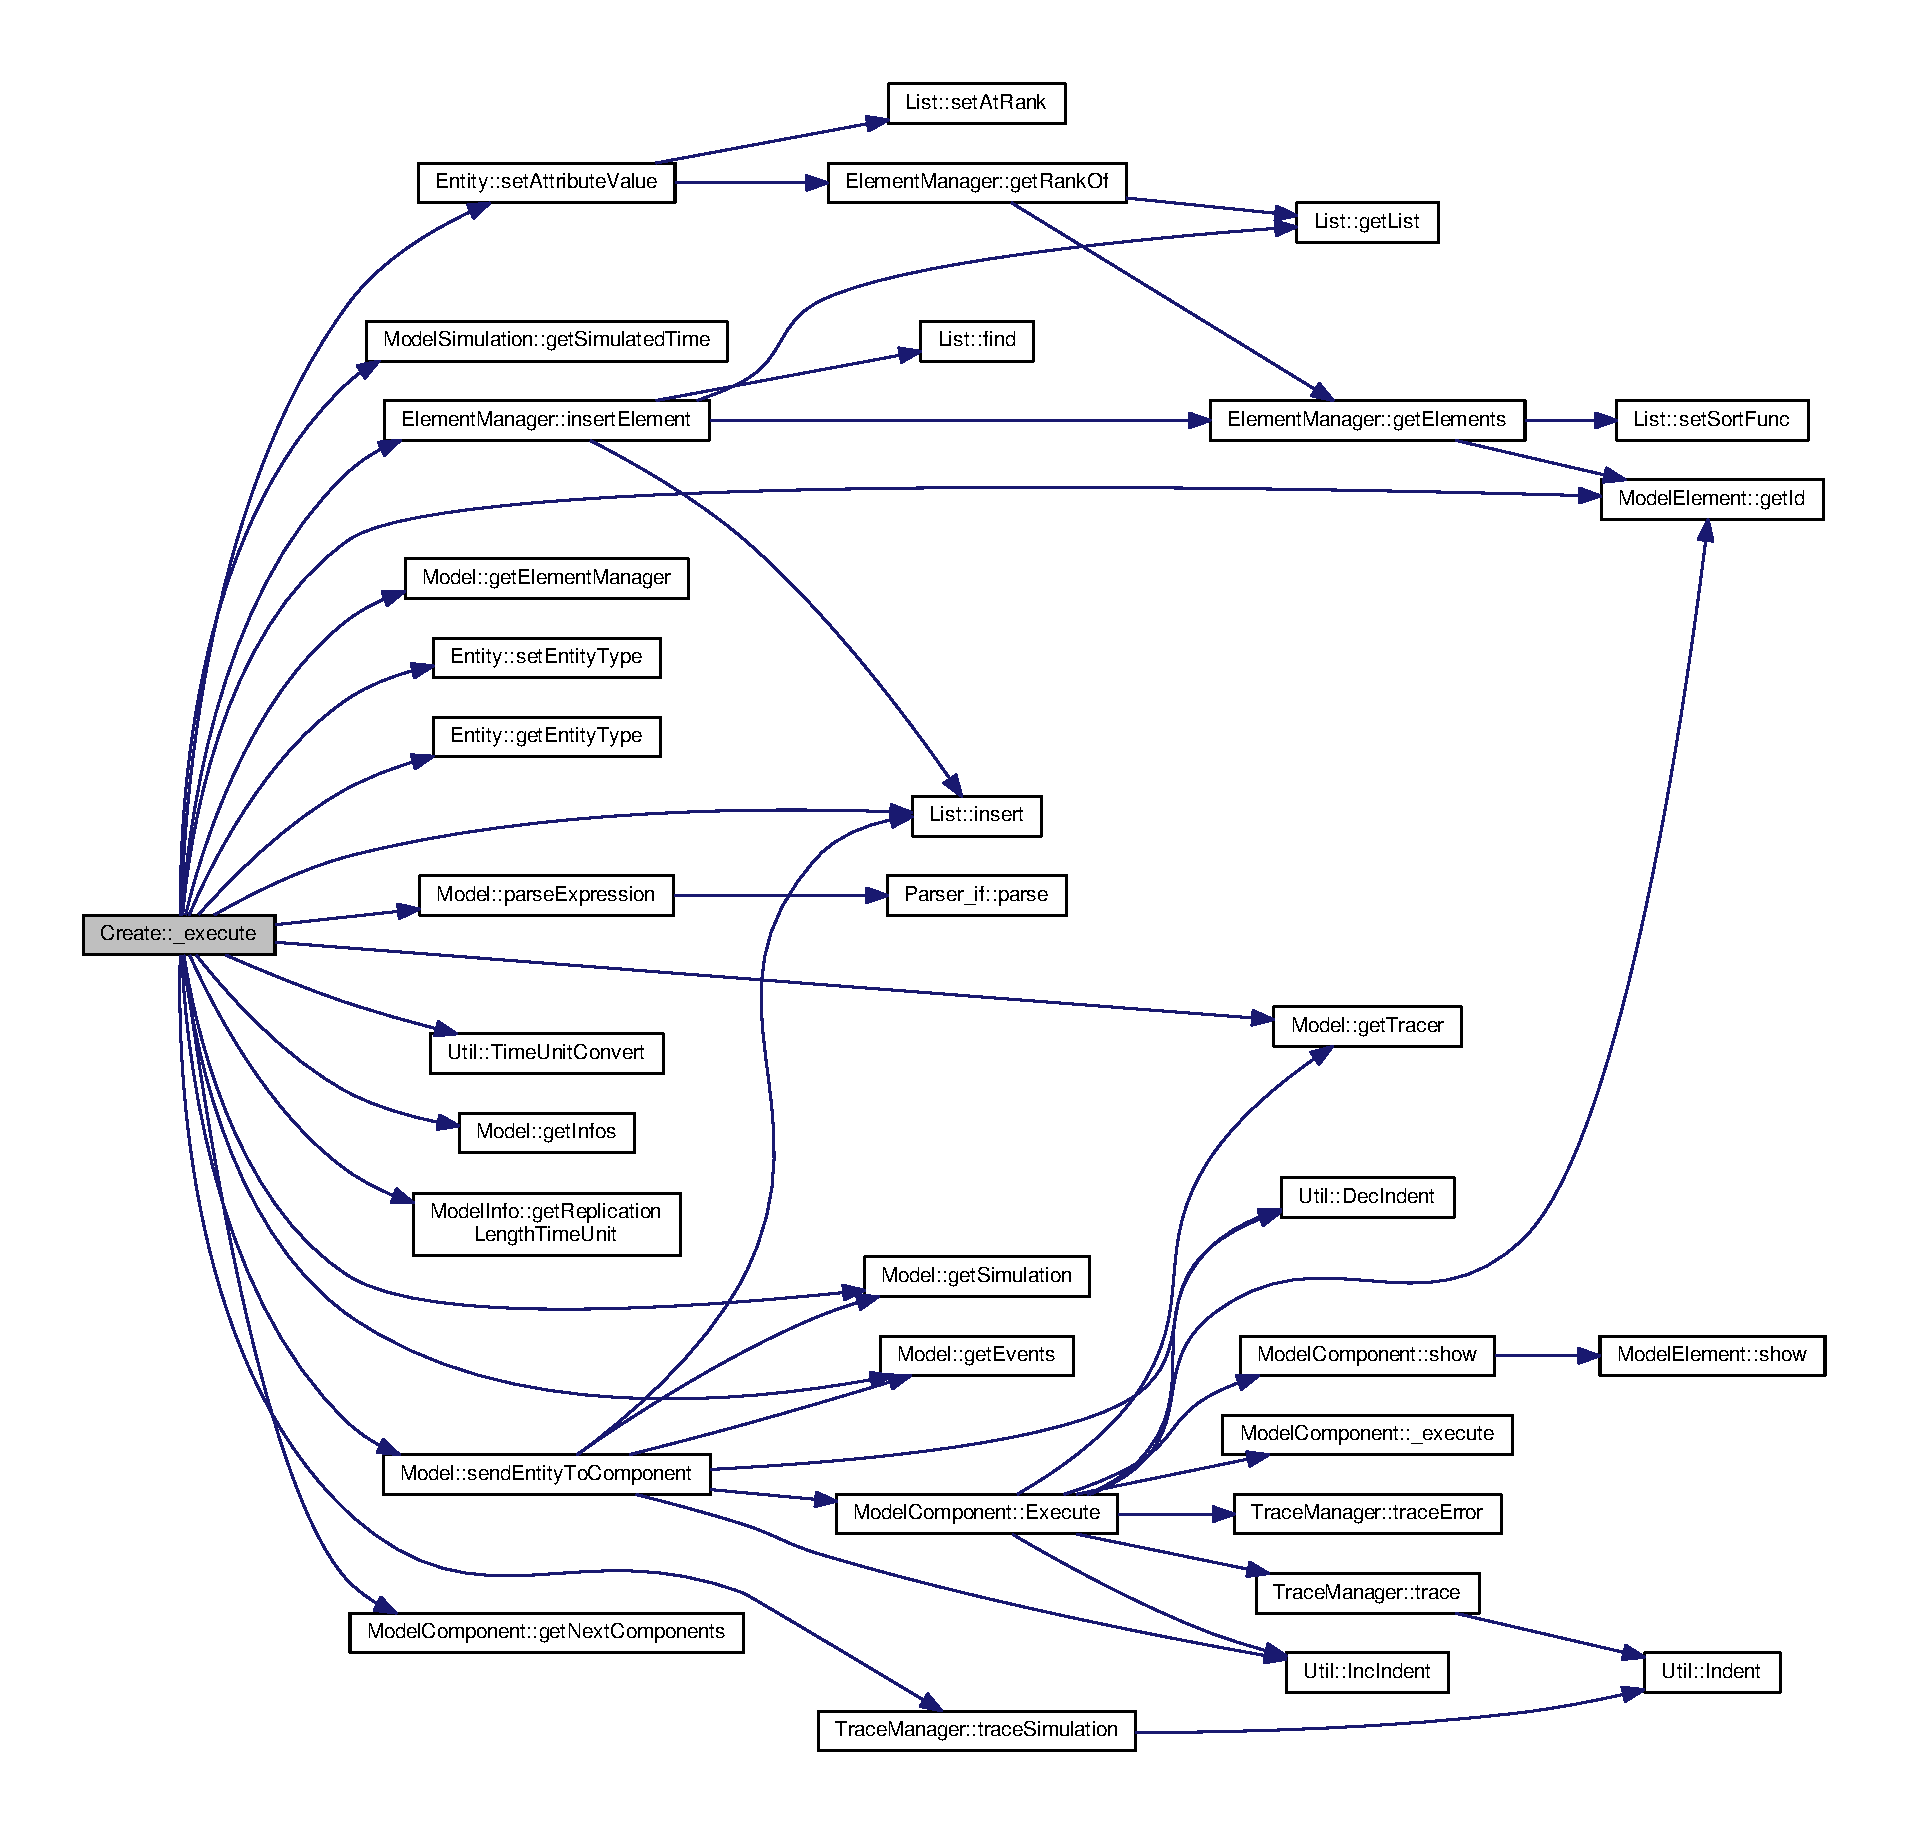
\includegraphics[width=350pt]{class_create_acd3a4b8805561591e0c88d3fd689cf74_cgraph}
\end{center}
\end{figure}


\index{Create@{Create}!\+\_\+load\+Instance@{\+\_\+load\+Instance}}
\index{\+\_\+load\+Instance@{\+\_\+load\+Instance}!Create@{Create}}
\subsubsection[{\texorpdfstring{\+\_\+load\+Instance(std\+::list$<$ std\+::string $>$ words)}{_loadInstance(std::list< std::string > words)}}]{\setlength{\rightskip}{0pt plus 5cm}void Create\+::\+\_\+load\+Instance (
\begin{DoxyParamCaption}
\item[{std\+::list$<$ std\+::string $>$}]{words}
\end{DoxyParamCaption}
)\hspace{0.3cm}{\ttfamily [protected]}, {\ttfamily [virtual]}}\hypertarget{class_create_aaa3cb1a4359586b0b8df817f57916286}{}\label{class_create_aaa3cb1a4359586b0b8df817f57916286}


Implements \hyperlink{class_model_element_a8208ee1dbd8b15acf7c2a0a85b218d56}{Model\+Element}.



Here is the call graph for this function\+:\nopagebreak
\begin{figure}[H]
\begin{center}
\leavevmode
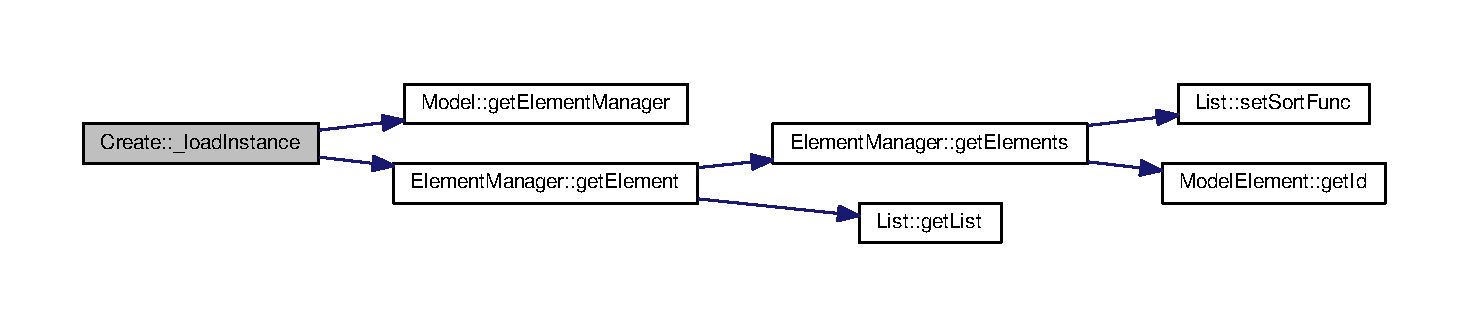
\includegraphics[width=350pt]{class_create_aaa3cb1a4359586b0b8df817f57916286_cgraph}
\end{center}
\end{figure}


\index{Create@{Create}!\+\_\+save\+Instance@{\+\_\+save\+Instance}}
\index{\+\_\+save\+Instance@{\+\_\+save\+Instance}!Create@{Create}}
\subsubsection[{\texorpdfstring{\+\_\+save\+Instance()}{_saveInstance()}}]{\setlength{\rightskip}{0pt plus 5cm}std\+::list$<$ std\+::string $>$ $\ast$ Create\+::\+\_\+save\+Instance (
\begin{DoxyParamCaption}
{}
\end{DoxyParamCaption}
)\hspace{0.3cm}{\ttfamily [protected]}, {\ttfamily [virtual]}}\hypertarget{class_create_ae1fd0c281cec35dcf91881acba8d7041}{}\label{class_create_ae1fd0c281cec35dcf91881acba8d7041}


Reimplemented from \hyperlink{class_model_component_a465f41c7191cb0fdf9039ef1f3d755a5}{Model\+Component}.



Here is the call graph for this function\+:\nopagebreak
\begin{figure}[H]
\begin{center}
\leavevmode
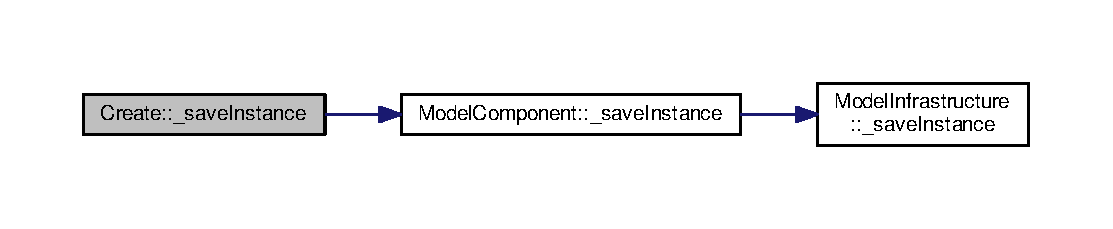
\includegraphics[width=350pt]{class_create_ae1fd0c281cec35dcf91881acba8d7041_cgraph}
\end{center}
\end{figure}


\index{Create@{Create}!\+\_\+verify\+Symbols@{\+\_\+verify\+Symbols}}
\index{\+\_\+verify\+Symbols@{\+\_\+verify\+Symbols}!Create@{Create}}
\subsubsection[{\texorpdfstring{\+\_\+verify\+Symbols(std\+::string $\ast$error\+Message)}{_verifySymbols(std::string *errorMessage)}}]{\setlength{\rightskip}{0pt plus 5cm}bool Create\+::\+\_\+verify\+Symbols (
\begin{DoxyParamCaption}
\item[{std\+::string $\ast$}]{error\+Message}
\end{DoxyParamCaption}
)\hspace{0.3cm}{\ttfamily [protected]}, {\ttfamily [virtual]}}\hypertarget{class_create_ad445fd3bec94b4e66669089f10f96057}{}\label{class_create_ad445fd3bec94b4e66669089f10f96057}


Implements \hyperlink{class_model_element_a42d23a83672cf746c709a031966484b2}{Model\+Element}.



Here is the call graph for this function\+:\nopagebreak
\begin{figure}[H]
\begin{center}
\leavevmode
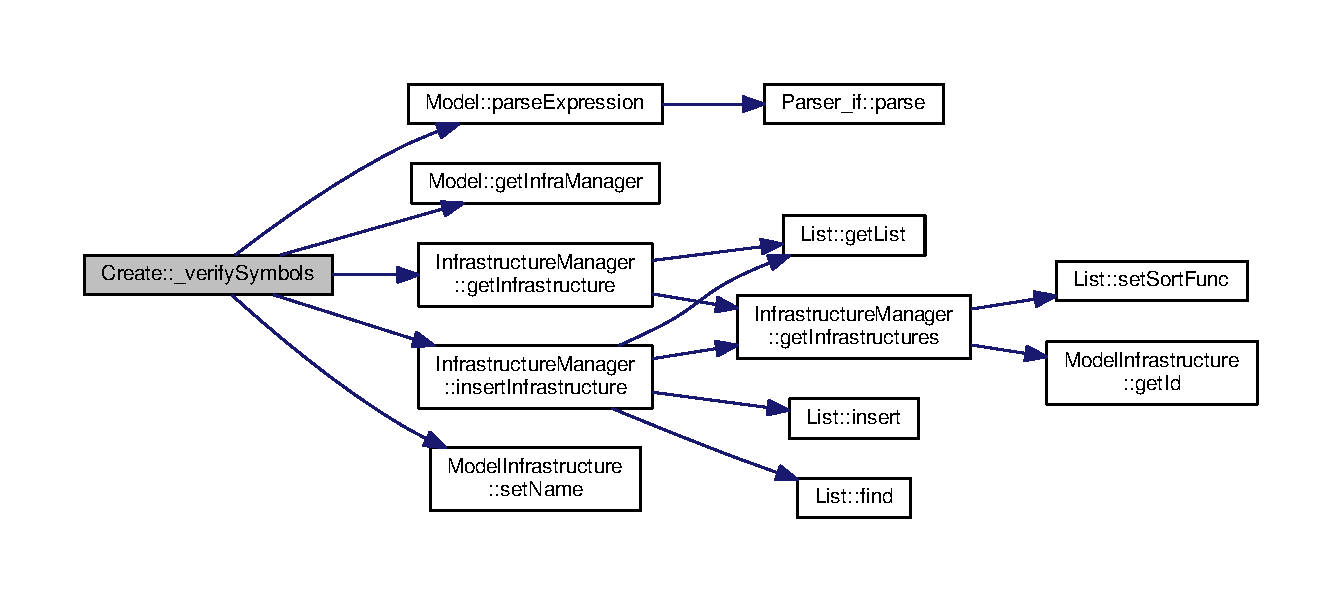
\includegraphics[width=350pt]{class_create_ad445fd3bec94b4e66669089f10f96057_cgraph}
\end{center}
\end{figure}


\index{Create@{Create}!show@{show}}
\index{show@{show}!Create@{Create}}
\subsubsection[{\texorpdfstring{show()}{show()}}]{\setlength{\rightskip}{0pt plus 5cm}std\+::string Create\+::show (
\begin{DoxyParamCaption}
{}
\end{DoxyParamCaption}
)\hspace{0.3cm}{\ttfamily [virtual]}}\hypertarget{class_create_a8d1832d2165bbeea4a5a88aded883f86}{}\label{class_create_a8d1832d2165bbeea4a5a88aded883f86}


Reimplemented from \hyperlink{class_source_model_component_a4011597b5780fcc0495e8e22ab8158f6}{Source\+Model\+Component}.



Here is the call graph for this function\+:\nopagebreak
\begin{figure}[H]
\begin{center}
\leavevmode
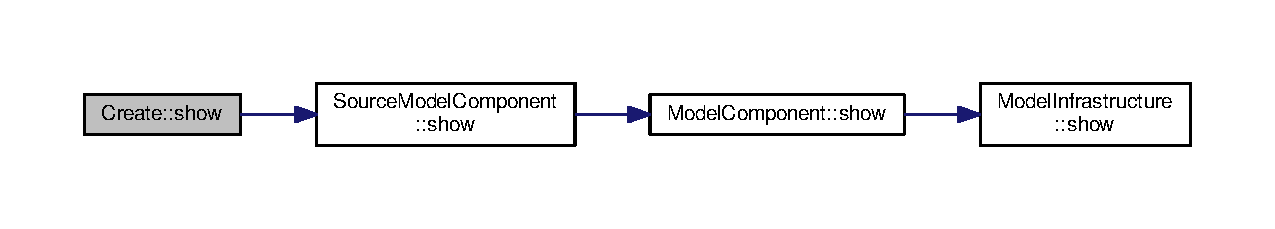
\includegraphics[width=350pt]{class_create_a8d1832d2165bbeea4a5a88aded883f86_cgraph}
\end{center}
\end{figure}




The documentation for this class was generated from the following files\+:\begin{DoxyCompactItemize}
\item 
\hyperlink{_create_8h}{Create.\+h}\item 
\hyperlink{_create_8cpp}{Create.\+cpp}\end{DoxyCompactItemize}

\hypertarget{class_decide}{}\section{Decide Class Reference}
\label{class_decide}\index{Decide@{Decide}}


{\ttfamily \#include $<$Decide.\+h$>$}



Inheritance diagram for Decide\+:\nopagebreak
\begin{figure}[H]
\begin{center}
\leavevmode
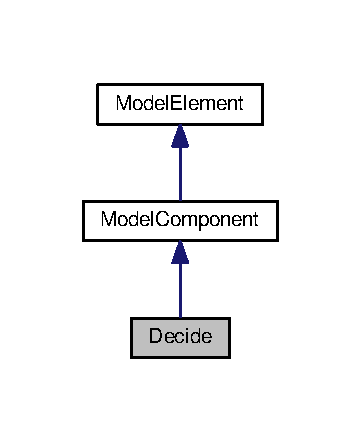
\includegraphics[width=173pt]{class_decide__inherit__graph}
\end{center}
\end{figure}


Collaboration diagram for Decide\+:\nopagebreak
\begin{figure}[H]
\begin{center}
\leavevmode
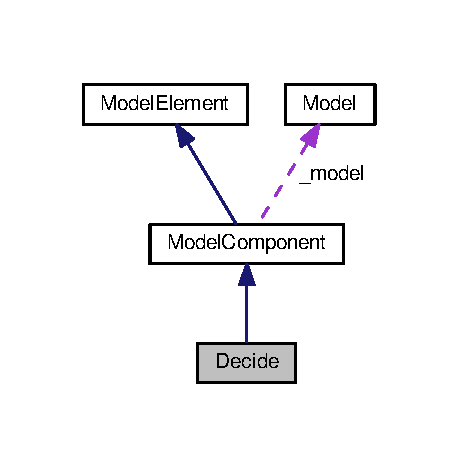
\includegraphics[width=220pt]{class_decide__coll__graph}
\end{center}
\end{figure}
\subsection*{Public Member Functions}
\begin{DoxyCompactItemize}
\item 
\hyperlink{class_decide_a7b3204637542be0a55c59e1396fae40b}{Decide} (\hyperlink{class_model}{Model} $\ast$model)
\item 
\hyperlink{class_decide_a5fe15a38389b322aa60c0862dae86b9b}{Decide} (const \hyperlink{class_decide}{Decide} \&orig)
\item 
virtual \hyperlink{class_decide_a2570a0531aa97aa29284a475d2929c1c}{$\sim$\+Decide} ()
\item 
\hyperlink{class_list}{List}$<$ std\+::string $>$ $\ast$ \hyperlink{class_decide_a6c9a4f0acff3d9f31568c0e5e966c86c}{get\+Conditions} () const 
\item 
virtual std\+::string \hyperlink{class_decide_a19e2a1143403795bcfd83903a1c0f695}{show} ()
\end{DoxyCompactItemize}
\subsection*{Protected Member Functions}
\begin{DoxyCompactItemize}
\item 
virtual void \hyperlink{class_decide_a873773c9e74e15a4dae52ef11c43b96c}{\+\_\+execute} (\hyperlink{class_entity}{Entity} $\ast$entity)
\item 
virtual void \hyperlink{class_decide_a0e6cfd81dd2a1aae9ae06a02ac86f201}{\+\_\+load\+Instance} (std\+::list$<$ std\+::string $>$ words)
\item 
virtual std\+::list$<$ std\+::string $>$ $\ast$ \hyperlink{class_decide_ae628db01a2a5583893bec28cc43fa29a}{\+\_\+save\+Instance} ()
\item 
virtual bool \hyperlink{class_decide_ac32726d32e89467a5c9a28e1af57f401}{\+\_\+verify\+Symbols} (std\+::string $\ast$error\+Message)
\end{DoxyCompactItemize}
\subsection*{Additional Inherited Members}


\subsection{Constructor \& Destructor Documentation}
\index{Decide@{Decide}!Decide@{Decide}}
\index{Decide@{Decide}!Decide@{Decide}}
\subsubsection[{\texorpdfstring{Decide(\+Model $\ast$model)}{Decide(Model *model)}}]{\setlength{\rightskip}{0pt plus 5cm}Decide\+::\+Decide (
\begin{DoxyParamCaption}
\item[{{\bf Model} $\ast$}]{model}
\end{DoxyParamCaption}
)}\hypertarget{class_decide_a7b3204637542be0a55c59e1396fae40b}{}\label{class_decide_a7b3204637542be0a55c59e1396fae40b}
\index{Decide@{Decide}!Decide@{Decide}}
\index{Decide@{Decide}!Decide@{Decide}}
\subsubsection[{\texorpdfstring{Decide(const Decide \&orig)}{Decide(const Decide &orig)}}]{\setlength{\rightskip}{0pt plus 5cm}Decide\+::\+Decide (
\begin{DoxyParamCaption}
\item[{const {\bf Decide} \&}]{orig}
\end{DoxyParamCaption}
)}\hypertarget{class_decide_a5fe15a38389b322aa60c0862dae86b9b}{}\label{class_decide_a5fe15a38389b322aa60c0862dae86b9b}
\index{Decide@{Decide}!````~Decide@{$\sim$\+Decide}}
\index{````~Decide@{$\sim$\+Decide}!Decide@{Decide}}
\subsubsection[{\texorpdfstring{$\sim$\+Decide()}{~Decide()}}]{\setlength{\rightskip}{0pt plus 5cm}Decide\+::$\sim$\+Decide (
\begin{DoxyParamCaption}
{}
\end{DoxyParamCaption}
)\hspace{0.3cm}{\ttfamily [virtual]}}\hypertarget{class_decide_a2570a0531aa97aa29284a475d2929c1c}{}\label{class_decide_a2570a0531aa97aa29284a475d2929c1c}


\subsection{Member Function Documentation}
\index{Decide@{Decide}!\+\_\+execute@{\+\_\+execute}}
\index{\+\_\+execute@{\+\_\+execute}!Decide@{Decide}}
\subsubsection[{\texorpdfstring{\+\_\+execute(\+Entity $\ast$entity)}{_execute(Entity *entity)}}]{\setlength{\rightskip}{0pt plus 5cm}void Decide\+::\+\_\+execute (
\begin{DoxyParamCaption}
\item[{{\bf Entity} $\ast$}]{entity}
\end{DoxyParamCaption}
)\hspace{0.3cm}{\ttfamily [protected]}, {\ttfamily [virtual]}}\hypertarget{class_decide_a873773c9e74e15a4dae52ef11c43b96c}{}\label{class_decide_a873773c9e74e15a4dae52ef11c43b96c}


Implements \hyperlink{class_model_component_ae3fcf8bbdd8368c882438424aa73f714}{Model\+Component}.



Here is the call graph for this function\+:\nopagebreak
\begin{figure}[H]
\begin{center}
\leavevmode
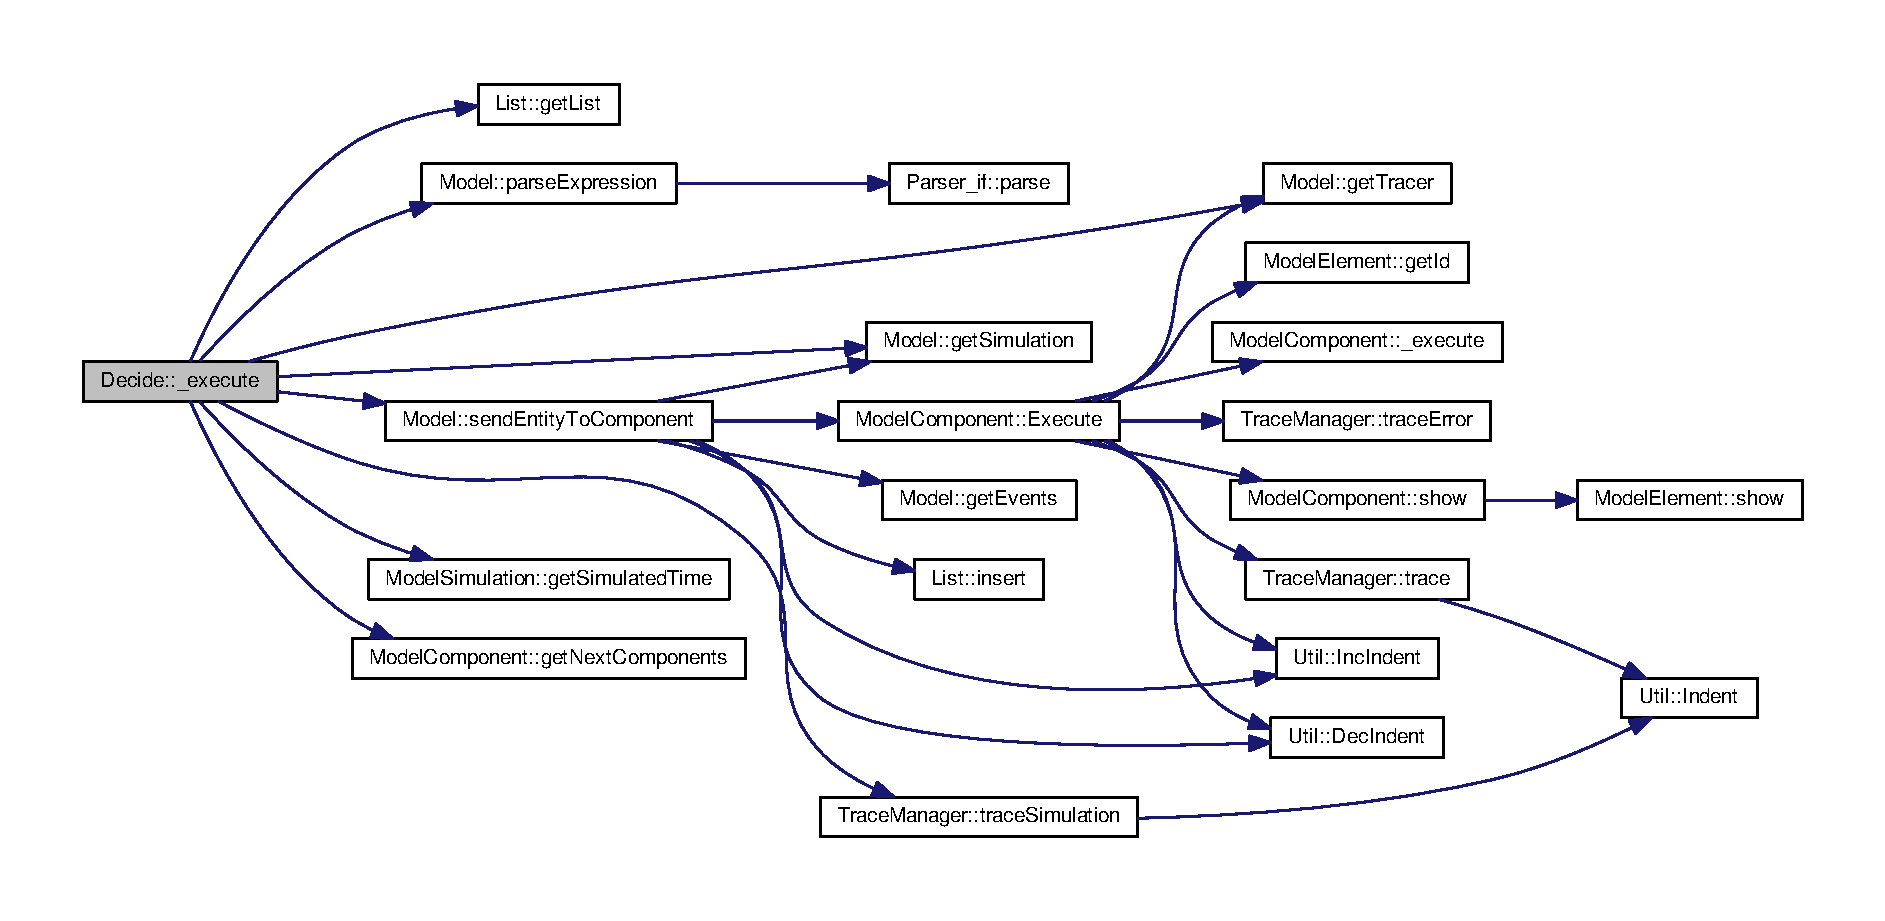
\includegraphics[width=350pt]{class_decide_a873773c9e74e15a4dae52ef11c43b96c_cgraph}
\end{center}
\end{figure}


\index{Decide@{Decide}!\+\_\+load\+Instance@{\+\_\+load\+Instance}}
\index{\+\_\+load\+Instance@{\+\_\+load\+Instance}!Decide@{Decide}}
\subsubsection[{\texorpdfstring{\+\_\+load\+Instance(std\+::list$<$ std\+::string $>$ words)}{_loadInstance(std::list< std::string > words)}}]{\setlength{\rightskip}{0pt plus 5cm}void Decide\+::\+\_\+load\+Instance (
\begin{DoxyParamCaption}
\item[{std\+::list$<$ std\+::string $>$}]{words}
\end{DoxyParamCaption}
)\hspace{0.3cm}{\ttfamily [protected]}, {\ttfamily [virtual]}}\hypertarget{class_decide_a0e6cfd81dd2a1aae9ae06a02ac86f201}{}\label{class_decide_a0e6cfd81dd2a1aae9ae06a02ac86f201}


Implements \hyperlink{class_model_element_a8208ee1dbd8b15acf7c2a0a85b218d56}{Model\+Element}.

\index{Decide@{Decide}!\+\_\+save\+Instance@{\+\_\+save\+Instance}}
\index{\+\_\+save\+Instance@{\+\_\+save\+Instance}!Decide@{Decide}}
\subsubsection[{\texorpdfstring{\+\_\+save\+Instance()}{_saveInstance()}}]{\setlength{\rightskip}{0pt plus 5cm}std\+::list$<$ std\+::string $>$ $\ast$ Decide\+::\+\_\+save\+Instance (
\begin{DoxyParamCaption}
{}
\end{DoxyParamCaption}
)\hspace{0.3cm}{\ttfamily [protected]}, {\ttfamily [virtual]}}\hypertarget{class_decide_ae628db01a2a5583893bec28cc43fa29a}{}\label{class_decide_ae628db01a2a5583893bec28cc43fa29a}


Reimplemented from \hyperlink{class_model_component_a465f41c7191cb0fdf9039ef1f3d755a5}{Model\+Component}.

\index{Decide@{Decide}!\+\_\+verify\+Symbols@{\+\_\+verify\+Symbols}}
\index{\+\_\+verify\+Symbols@{\+\_\+verify\+Symbols}!Decide@{Decide}}
\subsubsection[{\texorpdfstring{\+\_\+verify\+Symbols(std\+::string $\ast$error\+Message)}{_verifySymbols(std::string *errorMessage)}}]{\setlength{\rightskip}{0pt plus 5cm}bool Decide\+::\+\_\+verify\+Symbols (
\begin{DoxyParamCaption}
\item[{std\+::string $\ast$}]{error\+Message}
\end{DoxyParamCaption}
)\hspace{0.3cm}{\ttfamily [protected]}, {\ttfamily [virtual]}}\hypertarget{class_decide_ac32726d32e89467a5c9a28e1af57f401}{}\label{class_decide_ac32726d32e89467a5c9a28e1af57f401}


Implements \hyperlink{class_model_element_a42d23a83672cf746c709a031966484b2}{Model\+Element}.

\index{Decide@{Decide}!get\+Conditions@{get\+Conditions}}
\index{get\+Conditions@{get\+Conditions}!Decide@{Decide}}
\subsubsection[{\texorpdfstring{get\+Conditions() const }{getConditions() const }}]{\setlength{\rightskip}{0pt plus 5cm}{\bf List}$<$ std\+::string $>$ $\ast$ Decide\+::get\+Conditions (
\begin{DoxyParamCaption}
{}
\end{DoxyParamCaption}
) const}\hypertarget{class_decide_a6c9a4f0acff3d9f31568c0e5e966c86c}{}\label{class_decide_a6c9a4f0acff3d9f31568c0e5e966c86c}


Here is the caller graph for this function\+:\nopagebreak
\begin{figure}[H]
\begin{center}
\leavevmode
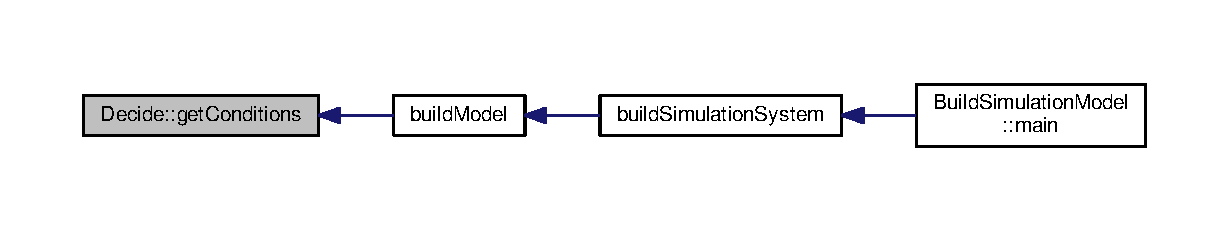
\includegraphics[width=350pt]{class_decide_a6c9a4f0acff3d9f31568c0e5e966c86c_icgraph}
\end{center}
\end{figure}


\index{Decide@{Decide}!show@{show}}
\index{show@{show}!Decide@{Decide}}
\subsubsection[{\texorpdfstring{show()}{show()}}]{\setlength{\rightskip}{0pt plus 5cm}std\+::string Decide\+::show (
\begin{DoxyParamCaption}
{}
\end{DoxyParamCaption}
)\hspace{0.3cm}{\ttfamily [virtual]}}\hypertarget{class_decide_a19e2a1143403795bcfd83903a1c0f695}{}\label{class_decide_a19e2a1143403795bcfd83903a1c0f695}


Reimplemented from \hyperlink{class_model_component_ad8bc846e36b028eab7efb7da6c549eca}{Model\+Component}.



The documentation for this class was generated from the following files\+:\begin{DoxyCompactItemize}
\item 
\hyperlink{_decide_8h}{Decide.\+h}\item 
\hyperlink{_decide_8cpp}{Decide.\+cpp}\end{DoxyCompactItemize}

\hypertarget{class_sampler_default_impl1_1_1_default_impl1_r_n_g___parameters}{}\section{Sampler\+Default\+Impl1\+:\+:Default\+Impl1\+R\+N\+G\+\_\+\+Parameters Class Reference}
\label{class_sampler_default_impl1_1_1_default_impl1_r_n_g___parameters}\index{Sampler\+Default\+Impl1\+::\+Default\+Impl1\+R\+N\+G\+\_\+\+Parameters@{Sampler\+Default\+Impl1\+::\+Default\+Impl1\+R\+N\+G\+\_\+\+Parameters}}


{\ttfamily \#include $<$Sampler\+Default\+Impl1.\+h$>$}



Inheritance diagram for Sampler\+Default\+Impl1\+:\+:Default\+Impl1\+R\+N\+G\+\_\+\+Parameters\+:\nopagebreak
\begin{figure}[H]
\begin{center}
\leavevmode
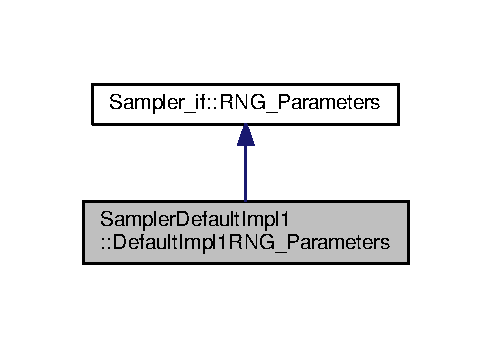
\includegraphics[width=236pt]{class_sampler_default_impl1_1_1_default_impl1_r_n_g___parameters__inherit__graph}
\end{center}
\end{figure}


Collaboration diagram for Sampler\+Default\+Impl1\+:\+:Default\+Impl1\+R\+N\+G\+\_\+\+Parameters\+:\nopagebreak
\begin{figure}[H]
\begin{center}
\leavevmode
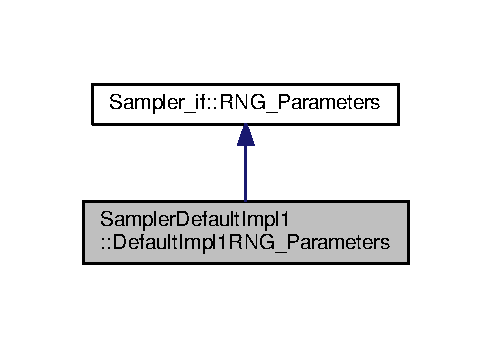
\includegraphics[width=236pt]{class_sampler_default_impl1_1_1_default_impl1_r_n_g___parameters__coll__graph}
\end{center}
\end{figure}
\subsection*{Public Attributes}
\begin{DoxyCompactItemize}
\item 
unsigned int \hyperlink{class_sampler_default_impl1_1_1_default_impl1_r_n_g___parameters_a32cf0e83a0b27a5f2cef15e8fdfe003e}{seed} = 666
\item 
unsigned int \hyperlink{class_sampler_default_impl1_1_1_default_impl1_r_n_g___parameters_ad6e4e6ffc3f62a1f837245edeee5e06d}{module} = 2147483647
\item 
unsigned int \hyperlink{class_sampler_default_impl1_1_1_default_impl1_r_n_g___parameters_a53063960d9de7d773e7e05af20ecd735}{multiplier} = 950706376
\end{DoxyCompactItemize}


\subsection{Member Data Documentation}
\index{Sampler\+Default\+Impl1\+::\+Default\+Impl1\+R\+N\+G\+\_\+\+Parameters@{Sampler\+Default\+Impl1\+::\+Default\+Impl1\+R\+N\+G\+\_\+\+Parameters}!module@{module}}
\index{module@{module}!Sampler\+Default\+Impl1\+::\+Default\+Impl1\+R\+N\+G\+\_\+\+Parameters@{Sampler\+Default\+Impl1\+::\+Default\+Impl1\+R\+N\+G\+\_\+\+Parameters}}
\subsubsection[{\texorpdfstring{module}{module}}]{\setlength{\rightskip}{0pt plus 5cm}unsigned int Sampler\+Default\+Impl1\+::\+Default\+Impl1\+R\+N\+G\+\_\+\+Parameters\+::module = 2147483647}\hypertarget{class_sampler_default_impl1_1_1_default_impl1_r_n_g___parameters_ad6e4e6ffc3f62a1f837245edeee5e06d}{}\label{class_sampler_default_impl1_1_1_default_impl1_r_n_g___parameters_ad6e4e6ffc3f62a1f837245edeee5e06d}
\index{Sampler\+Default\+Impl1\+::\+Default\+Impl1\+R\+N\+G\+\_\+\+Parameters@{Sampler\+Default\+Impl1\+::\+Default\+Impl1\+R\+N\+G\+\_\+\+Parameters}!multiplier@{multiplier}}
\index{multiplier@{multiplier}!Sampler\+Default\+Impl1\+::\+Default\+Impl1\+R\+N\+G\+\_\+\+Parameters@{Sampler\+Default\+Impl1\+::\+Default\+Impl1\+R\+N\+G\+\_\+\+Parameters}}
\subsubsection[{\texorpdfstring{multiplier}{multiplier}}]{\setlength{\rightskip}{0pt plus 5cm}unsigned int Sampler\+Default\+Impl1\+::\+Default\+Impl1\+R\+N\+G\+\_\+\+Parameters\+::multiplier = 950706376}\hypertarget{class_sampler_default_impl1_1_1_default_impl1_r_n_g___parameters_a53063960d9de7d773e7e05af20ecd735}{}\label{class_sampler_default_impl1_1_1_default_impl1_r_n_g___parameters_a53063960d9de7d773e7e05af20ecd735}
\index{Sampler\+Default\+Impl1\+::\+Default\+Impl1\+R\+N\+G\+\_\+\+Parameters@{Sampler\+Default\+Impl1\+::\+Default\+Impl1\+R\+N\+G\+\_\+\+Parameters}!seed@{seed}}
\index{seed@{seed}!Sampler\+Default\+Impl1\+::\+Default\+Impl1\+R\+N\+G\+\_\+\+Parameters@{Sampler\+Default\+Impl1\+::\+Default\+Impl1\+R\+N\+G\+\_\+\+Parameters}}
\subsubsection[{\texorpdfstring{seed}{seed}}]{\setlength{\rightskip}{0pt plus 5cm}unsigned int Sampler\+Default\+Impl1\+::\+Default\+Impl1\+R\+N\+G\+\_\+\+Parameters\+::seed = 666}\hypertarget{class_sampler_default_impl1_1_1_default_impl1_r_n_g___parameters_a32cf0e83a0b27a5f2cef15e8fdfe003e}{}\label{class_sampler_default_impl1_1_1_default_impl1_r_n_g___parameters_a32cf0e83a0b27a5f2cef15e8fdfe003e}


The documentation for this class was generated from the following file\+:\begin{DoxyCompactItemize}
\item 
\hyperlink{_sampler_default_impl1_8h}{Sampler\+Default\+Impl1.\+h}\end{DoxyCompactItemize}

\hypertarget{class_delay}{\section{Delay Class Reference}
\label{class_delay}\index{Delay@{Delay}}
}


{\ttfamily \#include $<$Delay.\-h$>$}



Inheritance diagram for Delay\-:\nopagebreak
\begin{figure}[H]
\begin{center}
\leavevmode
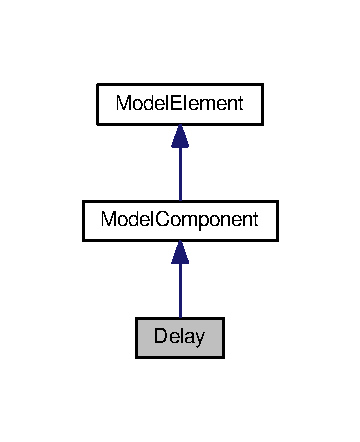
\includegraphics[width=180pt]{class_delay__inherit__graph}
\end{center}
\end{figure}


Collaboration diagram for Delay\-:\nopagebreak
\begin{figure}[H]
\begin{center}
\leavevmode
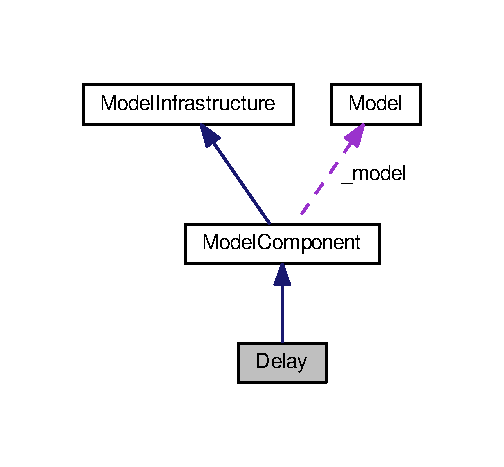
\includegraphics[width=241pt]{class_delay__coll__graph}
\end{center}
\end{figure}
\subsection*{Public Member Functions}
\begin{DoxyCompactItemize}
\item 
\hyperlink{class_delay_a155ad32911b3289d968cca746f940520}{Delay} (\hyperlink{class_model}{Model} $\ast$model)
\item 
\hyperlink{class_delay_a5892fd8feb283f11980c0a9adb9befa7}{Delay} (const \hyperlink{class_delay}{Delay} \&orig)
\item 
virtual \hyperlink{class_delay_afee934130955d45563a6c5baaaf052d2}{$\sim$\-Delay} ()
\item 
void \hyperlink{class_delay_a683b53af607a424477acb946eb3afdfc}{set\-Delay\-Expression} (std\-::string \-\_\-delay\-Expression)
\item 
std\-::string \hyperlink{class_delay_a58559eda9ed25330d29b967c1bb0add5}{get\-Delay\-Expression} () const 
\item 
void \hyperlink{class_delay_abe7e89dba0974a81d00e6d2c0548fc1e}{set\-Delay\-Time\-Unit} (\hyperlink{class_util_aadbd82055afeaa7d4fb4da513de628ff}{Util\-::\-Time\-Unit} \-\_\-delay\-Time\-Unit)
\item 
\hyperlink{class_util_aadbd82055afeaa7d4fb4da513de628ff}{Util\-::\-Time\-Unit} \hyperlink{class_delay_a0561a6fdb4dd317952b5bb8d87b0c15f}{get\-Delay\-Time\-Unit} () const 
\item 
virtual std\-::string \hyperlink{class_delay_af8187e4515417b547dc22b5ee0a1f95d}{show} ()
\end{DoxyCompactItemize}
\subsection*{Protected Member Functions}
\begin{DoxyCompactItemize}
\item 
virtual void \hyperlink{class_delay_a029d91a2cd736ff9c361c69336e6ab41}{\-\_\-execute} (\hyperlink{class_entity}{Entity} $\ast$entity)
\item 
virtual void \hyperlink{class_delay_acd33d05fc1c8d6d66a6f674e49ee7c61}{\-\_\-load\-Instance} (std\-::list$<$ std\-::string $>$ words)
\item 
virtual std\-::list$<$ std\-::string $>$ $\ast$ \hyperlink{class_delay_a73676f11cddd31439a407b5dabcea43a}{\-\_\-save\-Instance} ()
\item 
virtual bool \hyperlink{class_delay_af1690df9ba58e9972f5721f5bdc2b520}{\-\_\-verify\-Symbols} (std\-::string $\ast$error\-Message)
\end{DoxyCompactItemize}
\subsection*{Additional Inherited Members}


\subsection{Detailed Description}


Definition at line 20 of file Delay.\-h.



\subsection{Constructor \& Destructor Documentation}
\hypertarget{class_delay_a155ad32911b3289d968cca746f940520}{\index{Delay@{Delay}!Delay@{Delay}}
\index{Delay@{Delay}!Delay@{Delay}}
\subsubsection[{Delay}]{\setlength{\rightskip}{0pt plus 5cm}Delay\-::\-Delay (
\begin{DoxyParamCaption}
\item[{{\bf Model} $\ast$}]{model}
\end{DoxyParamCaption}
)}}\label{class_delay_a155ad32911b3289d968cca746f940520}


Definition at line 17 of file Delay.\-cpp.

\hypertarget{class_delay_a5892fd8feb283f11980c0a9adb9befa7}{\index{Delay@{Delay}!Delay@{Delay}}
\index{Delay@{Delay}!Delay@{Delay}}
\subsubsection[{Delay}]{\setlength{\rightskip}{0pt plus 5cm}Delay\-::\-Delay (
\begin{DoxyParamCaption}
\item[{const {\bf Delay} \&}]{orig}
\end{DoxyParamCaption}
)}}\label{class_delay_a5892fd8feb283f11980c0a9adb9befa7}


Definition at line 21 of file Delay.\-cpp.

\hypertarget{class_delay_afee934130955d45563a6c5baaaf052d2}{\index{Delay@{Delay}!$\sim$\-Delay@{$\sim$\-Delay}}
\index{$\sim$\-Delay@{$\sim$\-Delay}!Delay@{Delay}}
\subsubsection[{$\sim$\-Delay}]{\setlength{\rightskip}{0pt plus 5cm}Delay\-::$\sim$\-Delay (
\begin{DoxyParamCaption}
{}
\end{DoxyParamCaption}
)\hspace{0.3cm}{\ttfamily [virtual]}}}\label{class_delay_afee934130955d45563a6c5baaaf052d2}


Definition at line 24 of file Delay.\-cpp.



\subsection{Member Function Documentation}
\hypertarget{class_delay_a029d91a2cd736ff9c361c69336e6ab41}{\index{Delay@{Delay}!\-\_\-execute@{\-\_\-execute}}
\index{\-\_\-execute@{\-\_\-execute}!Delay@{Delay}}
\subsubsection[{\-\_\-execute}]{\setlength{\rightskip}{0pt plus 5cm}void Delay\-::\-\_\-execute (
\begin{DoxyParamCaption}
\item[{{\bf Entity} $\ast$}]{entity}
\end{DoxyParamCaption}
)\hspace{0.3cm}{\ttfamily [protected]}, {\ttfamily [virtual]}}}\label{class_delay_a029d91a2cd736ff9c361c69336e6ab41}


Implements \hyperlink{class_model_component_ae3fcf8bbdd8368c882438424aa73f714}{Model\-Component}.



Definition at line 49 of file Delay.\-cpp.



Here is the call graph for this function\-:\nopagebreak
\begin{figure}[H]
\begin{center}
\leavevmode
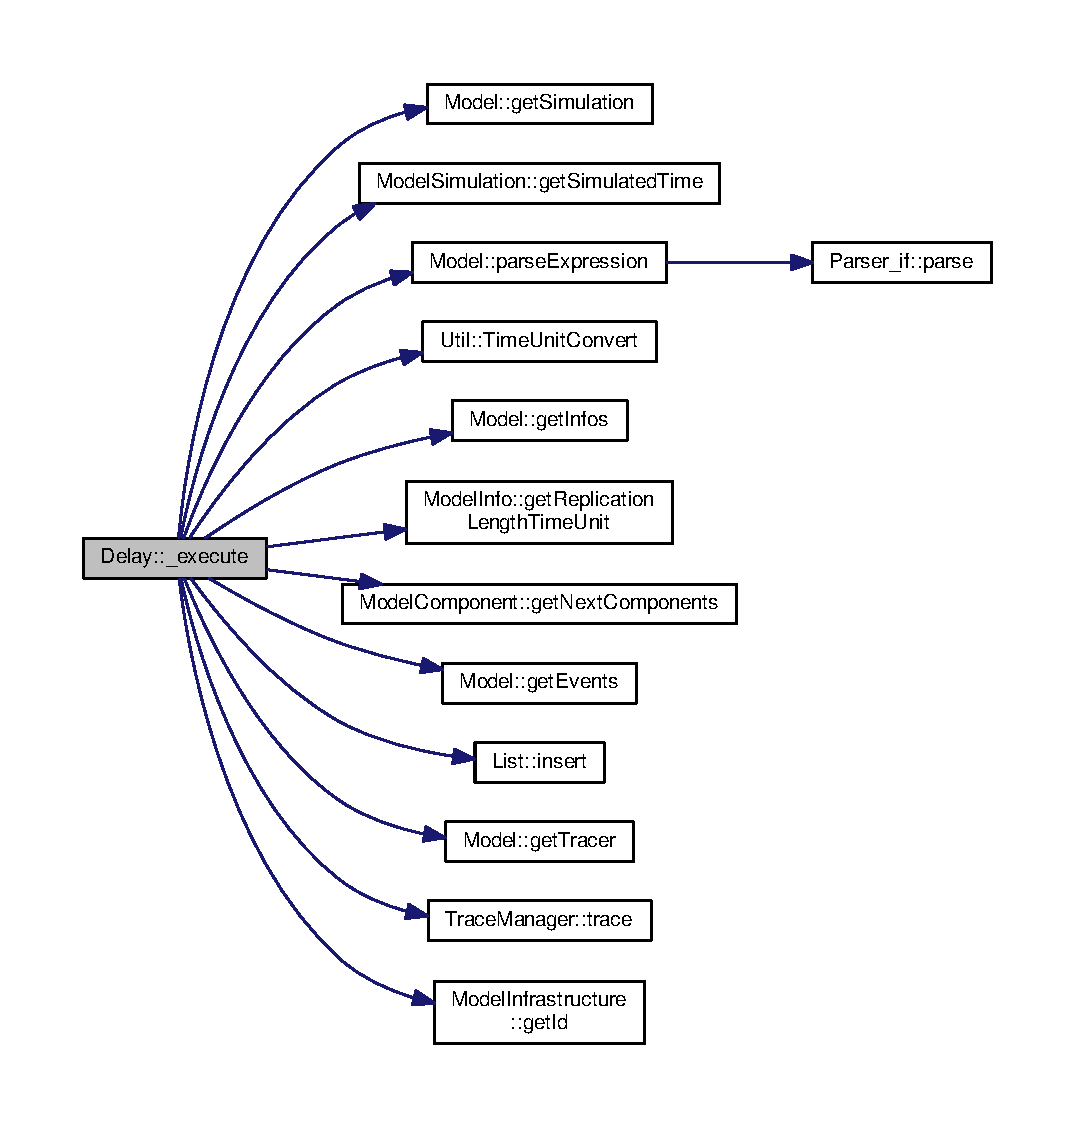
\includegraphics[width=350pt]{class_delay_a029d91a2cd736ff9c361c69336e6ab41_cgraph}
\end{center}
\end{figure}


\hypertarget{class_delay_acd33d05fc1c8d6d66a6f674e49ee7c61}{\index{Delay@{Delay}!\-\_\-load\-Instance@{\-\_\-load\-Instance}}
\index{\-\_\-load\-Instance@{\-\_\-load\-Instance}!Delay@{Delay}}
\subsubsection[{\-\_\-load\-Instance}]{\setlength{\rightskip}{0pt plus 5cm}void Delay\-::\-\_\-load\-Instance (
\begin{DoxyParamCaption}
\item[{std\-::list$<$ std\-::string $>$}]{words}
\end{DoxyParamCaption}
)\hspace{0.3cm}{\ttfamily [protected]}, {\ttfamily [virtual]}}}\label{class_delay_acd33d05fc1c8d6d66a6f674e49ee7c61}


Implements \hyperlink{class_model_infrastructure_ae118c8ad2ac9d4397c40d004af51b2dc}{Model\-Infrastructure}.



Definition at line 58 of file Delay.\-cpp.

\hypertarget{class_delay_a73676f11cddd31439a407b5dabcea43a}{\index{Delay@{Delay}!\-\_\-save\-Instance@{\-\_\-save\-Instance}}
\index{\-\_\-save\-Instance@{\-\_\-save\-Instance}!Delay@{Delay}}
\subsubsection[{\-\_\-save\-Instance}]{\setlength{\rightskip}{0pt plus 5cm}std\-::list$<$ std\-::string $>$ $\ast$ Delay\-::\-\_\-save\-Instance (
\begin{DoxyParamCaption}
{}
\end{DoxyParamCaption}
)\hspace{0.3cm}{\ttfamily [protected]}, {\ttfamily [virtual]}}}\label{class_delay_a73676f11cddd31439a407b5dabcea43a}


Implements \hyperlink{class_model_infrastructure_a3da2fd381c44752598bc448b207e8287}{Model\-Infrastructure}.



Definition at line 62 of file Delay.\-cpp.

\hypertarget{class_delay_af1690df9ba58e9972f5721f5bdc2b520}{\index{Delay@{Delay}!\-\_\-verify\-Symbols@{\-\_\-verify\-Symbols}}
\index{\-\_\-verify\-Symbols@{\-\_\-verify\-Symbols}!Delay@{Delay}}
\subsubsection[{\-\_\-verify\-Symbols}]{\setlength{\rightskip}{0pt plus 5cm}bool Delay\-::\-\_\-verify\-Symbols (
\begin{DoxyParamCaption}
\item[{std\-::string $\ast$}]{error\-Message}
\end{DoxyParamCaption}
)\hspace{0.3cm}{\ttfamily [protected]}, {\ttfamily [virtual]}}}\label{class_delay_af1690df9ba58e9972f5721f5bdc2b520}


Implements \hyperlink{class_model_infrastructure_a43de089b35b96c32dd24ca4f9636a388}{Model\-Infrastructure}.



Definition at line 68 of file Delay.\-cpp.

\hypertarget{class_delay_a58559eda9ed25330d29b967c1bb0add5}{\index{Delay@{Delay}!get\-Delay\-Expression@{get\-Delay\-Expression}}
\index{get\-Delay\-Expression@{get\-Delay\-Expression}!Delay@{Delay}}
\subsubsection[{get\-Delay\-Expression}]{\setlength{\rightskip}{0pt plus 5cm}std\-::string Delay\-::get\-Delay\-Expression (
\begin{DoxyParamCaption}
{}
\end{DoxyParamCaption}
) const}}\label{class_delay_a58559eda9ed25330d29b967c1bb0add5}


Definition at line 37 of file Delay.\-cpp.

\hypertarget{class_delay_a0561a6fdb4dd317952b5bb8d87b0c15f}{\index{Delay@{Delay}!get\-Delay\-Time\-Unit@{get\-Delay\-Time\-Unit}}
\index{get\-Delay\-Time\-Unit@{get\-Delay\-Time\-Unit}!Delay@{Delay}}
\subsubsection[{get\-Delay\-Time\-Unit}]{\setlength{\rightskip}{0pt plus 5cm}{\bf Util\-::\-Time\-Unit} Delay\-::get\-Delay\-Time\-Unit (
\begin{DoxyParamCaption}
{}
\end{DoxyParamCaption}
) const}}\label{class_delay_a0561a6fdb4dd317952b5bb8d87b0c15f}


Definition at line 45 of file Delay.\-cpp.

\hypertarget{class_delay_a683b53af607a424477acb946eb3afdfc}{\index{Delay@{Delay}!set\-Delay\-Expression@{set\-Delay\-Expression}}
\index{set\-Delay\-Expression@{set\-Delay\-Expression}!Delay@{Delay}}
\subsubsection[{set\-Delay\-Expression}]{\setlength{\rightskip}{0pt plus 5cm}void Delay\-::set\-Delay\-Expression (
\begin{DoxyParamCaption}
\item[{std\-::string}]{\-\_\-delay\-Expression}
\end{DoxyParamCaption}
)}}\label{class_delay_a683b53af607a424477acb946eb3afdfc}


Definition at line 33 of file Delay.\-cpp.



Here is the caller graph for this function\-:\nopagebreak
\begin{figure}[H]
\begin{center}
\leavevmode
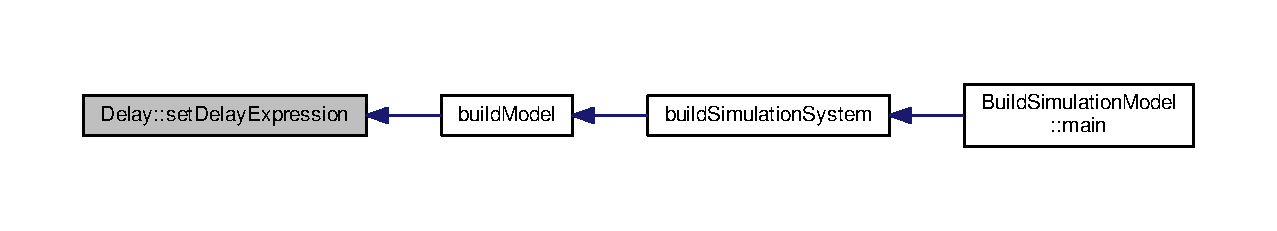
\includegraphics[width=350pt]{class_delay_a683b53af607a424477acb946eb3afdfc_icgraph}
\end{center}
\end{figure}


\hypertarget{class_delay_abe7e89dba0974a81d00e6d2c0548fc1e}{\index{Delay@{Delay}!set\-Delay\-Time\-Unit@{set\-Delay\-Time\-Unit}}
\index{set\-Delay\-Time\-Unit@{set\-Delay\-Time\-Unit}!Delay@{Delay}}
\subsubsection[{set\-Delay\-Time\-Unit}]{\setlength{\rightskip}{0pt plus 5cm}void Delay\-::set\-Delay\-Time\-Unit (
\begin{DoxyParamCaption}
\item[{{\bf Util\-::\-Time\-Unit}}]{\-\_\-delay\-Time\-Unit}
\end{DoxyParamCaption}
)}}\label{class_delay_abe7e89dba0974a81d00e6d2c0548fc1e}


Definition at line 41 of file Delay.\-cpp.

\hypertarget{class_delay_af8187e4515417b547dc22b5ee0a1f95d}{\index{Delay@{Delay}!show@{show}}
\index{show@{show}!Delay@{Delay}}
\subsubsection[{show}]{\setlength{\rightskip}{0pt plus 5cm}std\-::string Delay\-::show (
\begin{DoxyParamCaption}
{}
\end{DoxyParamCaption}
)\hspace{0.3cm}{\ttfamily [virtual]}}}\label{class_delay_af8187e4515417b547dc22b5ee0a1f95d}


Reimplemented from \hyperlink{class_model_component_ad8bc846e36b028eab7efb7da6c549eca}{Model\-Component}.



Definition at line 27 of file Delay.\-cpp.



Here is the call graph for this function\-:\nopagebreak
\begin{figure}[H]
\begin{center}
\leavevmode
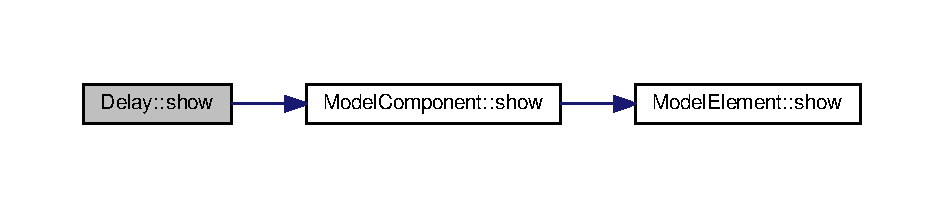
\includegraphics[width=350pt]{class_delay_af8187e4515417b547dc22b5ee0a1f95d_cgraph}
\end{center}
\end{figure}




The documentation for this class was generated from the following files\-:\begin{DoxyCompactItemize}
\item 
\hyperlink{_delay_8h}{Delay.\-h}\item 
\hyperlink{_delay_8cpp}{Delay.\-cpp}\end{DoxyCompactItemize}

\hypertarget{class_dispose}{}\section{Dispose Class Reference}
\label{class_dispose}\index{Dispose@{Dispose}}


{\ttfamily \#include $<$Dispose.\+h$>$}



Inheritance diagram for Dispose\+:
\nopagebreak
\begin{figure}[H]
\begin{center}
\leavevmode
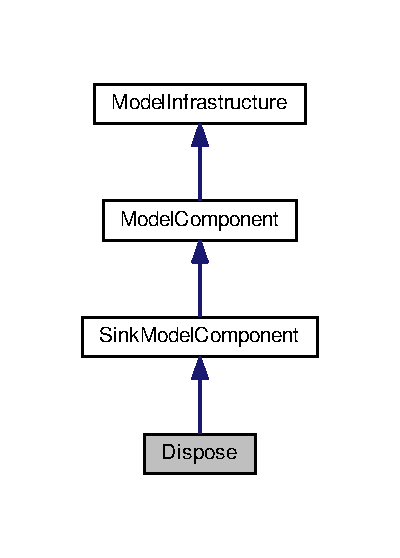
\includegraphics[width=193pt]{class_dispose__inherit__graph}
\end{center}
\end{figure}


Collaboration diagram for Dispose\+:
\nopagebreak
\begin{figure}[H]
\begin{center}
\leavevmode
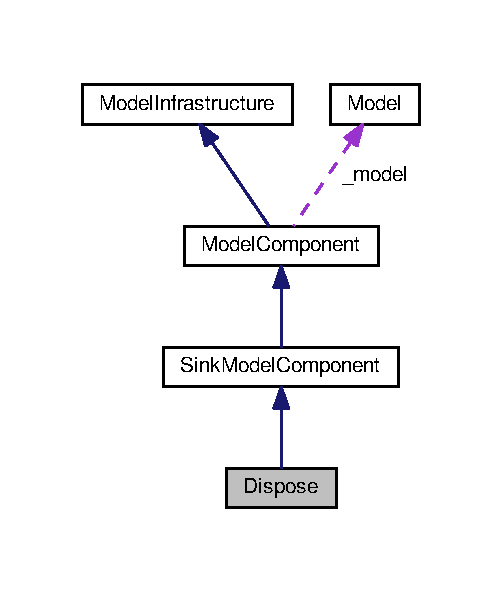
\includegraphics[width=242pt]{class_dispose__coll__graph}
\end{center}
\end{figure}
\subsection*{Public Member Functions}
\begin{DoxyCompactItemize}
\item 
\hyperlink{class_dispose_a9b5ccd61252e7f36d747fd832debdfaa}{Dispose} (\hyperlink{class_model}{Model} $\ast$model)
\item 
\hyperlink{class_dispose_a8d4515962baf1fd7c01912cb654aa683}{Dispose} (const \hyperlink{class_dispose}{Dispose} \&orig)
\item 
virtual \hyperlink{class_dispose_a2a2af23e9cbca66b02a142252a99096d}{$\sim$\+Dispose} ()
\item 
virtual std\+::string \hyperlink{class_dispose_aee8ef98d5ca22eb18a97b258ed059865}{show} ()
\item 
void \hyperlink{class_dispose_a8dc978664e640bc4d58760770b84b84e}{set\+Collect\+Statistics} (bool \+\_\+collect\+Statistics)
\item 
bool \hyperlink{class_dispose_aff15fbea8737b30efe9b3521d12350bd}{is\+Collect\+Statistics} () const 
\end{DoxyCompactItemize}
\subsection*{Protected Member Functions}
\begin{DoxyCompactItemize}
\item 
virtual void \hyperlink{class_dispose_a342eb428496534cdfd17524ad78b0c08}{\+\_\+execute} (\hyperlink{class_entity}{Entity} $\ast$entity)
\item 
virtual void \hyperlink{class_dispose_a245f73bff07925e3efc1eeffd84c9ac6}{\+\_\+load\+Instance} (std\+::list$<$ std\+::string $>$ words)
\item 
virtual std\+::list$<$ std\+::string $>$ $\ast$ \hyperlink{class_dispose_ae12482052fb78fa534dda5d4c0a74e3e}{\+\_\+save\+Instance} ()
\item 
virtual bool \hyperlink{class_dispose_a5ad64b97bbb16662aa9d914eda2a7e38}{\+\_\+verify\+Symbols} (std\+::string $\ast$error\+Message)
\end{DoxyCompactItemize}
\subsection*{Additional Inherited Members}


\subsection{Constructor \& Destructor Documentation}
\index{Dispose@{Dispose}!Dispose@{Dispose}}
\index{Dispose@{Dispose}!Dispose@{Dispose}}
\subsubsection[{\texorpdfstring{Dispose(\+Model $\ast$model)}{Dispose(Model *model)}}]{\setlength{\rightskip}{0pt plus 5cm}Dispose\+::\+Dispose (
\begin{DoxyParamCaption}
\item[{{\bf Model} $\ast$}]{model}
\end{DoxyParamCaption}
)}\hypertarget{class_dispose_a9b5ccd61252e7f36d747fd832debdfaa}{}\label{class_dispose_a9b5ccd61252e7f36d747fd832debdfaa}
\index{Dispose@{Dispose}!Dispose@{Dispose}}
\index{Dispose@{Dispose}!Dispose@{Dispose}}
\subsubsection[{\texorpdfstring{Dispose(const Dispose \&orig)}{Dispose(const Dispose &orig)}}]{\setlength{\rightskip}{0pt plus 5cm}Dispose\+::\+Dispose (
\begin{DoxyParamCaption}
\item[{const {\bf Dispose} \&}]{orig}
\end{DoxyParamCaption}
)}\hypertarget{class_dispose_a8d4515962baf1fd7c01912cb654aa683}{}\label{class_dispose_a8d4515962baf1fd7c01912cb654aa683}
\index{Dispose@{Dispose}!````~Dispose@{$\sim$\+Dispose}}
\index{````~Dispose@{$\sim$\+Dispose}!Dispose@{Dispose}}
\subsubsection[{\texorpdfstring{$\sim$\+Dispose()}{~Dispose()}}]{\setlength{\rightskip}{0pt plus 5cm}Dispose\+::$\sim$\+Dispose (
\begin{DoxyParamCaption}
{}
\end{DoxyParamCaption}
)\hspace{0.3cm}{\ttfamily [virtual]}}\hypertarget{class_dispose_a2a2af23e9cbca66b02a142252a99096d}{}\label{class_dispose_a2a2af23e9cbca66b02a142252a99096d}


\subsection{Member Function Documentation}
\index{Dispose@{Dispose}!\+\_\+execute@{\+\_\+execute}}
\index{\+\_\+execute@{\+\_\+execute}!Dispose@{Dispose}}
\subsubsection[{\texorpdfstring{\+\_\+execute(\+Entity $\ast$entity)}{_execute(Entity *entity)}}]{\setlength{\rightskip}{0pt plus 5cm}void Dispose\+::\+\_\+execute (
\begin{DoxyParamCaption}
\item[{{\bf Entity} $\ast$}]{entity}
\end{DoxyParamCaption}
)\hspace{0.3cm}{\ttfamily [protected]}, {\ttfamily [virtual]}}\hypertarget{class_dispose_a342eb428496534cdfd17524ad78b0c08}{}\label{class_dispose_a342eb428496534cdfd17524ad78b0c08}


Implements \hyperlink{class_model_component_ae3fcf8bbdd8368c882438424aa73f714}{Model\+Component}.

\index{Dispose@{Dispose}!\+\_\+load\+Instance@{\+\_\+load\+Instance}}
\index{\+\_\+load\+Instance@{\+\_\+load\+Instance}!Dispose@{Dispose}}
\subsubsection[{\texorpdfstring{\+\_\+load\+Instance(std\+::list$<$ std\+::string $>$ words)}{_loadInstance(std::list< std::string > words)}}]{\setlength{\rightskip}{0pt plus 5cm}void Dispose\+::\+\_\+load\+Instance (
\begin{DoxyParamCaption}
\item[{std\+::list$<$ std\+::string $>$}]{words}
\end{DoxyParamCaption}
)\hspace{0.3cm}{\ttfamily [protected]}, {\ttfamily [virtual]}}\hypertarget{class_dispose_a245f73bff07925e3efc1eeffd84c9ac6}{}\label{class_dispose_a245f73bff07925e3efc1eeffd84c9ac6}


Implements \hyperlink{class_model_infrastructure_ae118c8ad2ac9d4397c40d004af51b2dc}{Model\+Infrastructure}.

\index{Dispose@{Dispose}!\+\_\+save\+Instance@{\+\_\+save\+Instance}}
\index{\+\_\+save\+Instance@{\+\_\+save\+Instance}!Dispose@{Dispose}}
\subsubsection[{\texorpdfstring{\+\_\+save\+Instance()}{_saveInstance()}}]{\setlength{\rightskip}{0pt plus 5cm}std\+::list$<$ std\+::string $>$ $\ast$ Dispose\+::\+\_\+save\+Instance (
\begin{DoxyParamCaption}
{}
\end{DoxyParamCaption}
)\hspace{0.3cm}{\ttfamily [protected]}, {\ttfamily [virtual]}}\hypertarget{class_dispose_ae12482052fb78fa534dda5d4c0a74e3e}{}\label{class_dispose_ae12482052fb78fa534dda5d4c0a74e3e}


Reimplemented from \hyperlink{class_model_component_a465f41c7191cb0fdf9039ef1f3d755a5}{Model\+Component}.

\index{Dispose@{Dispose}!\+\_\+verify\+Symbols@{\+\_\+verify\+Symbols}}
\index{\+\_\+verify\+Symbols@{\+\_\+verify\+Symbols}!Dispose@{Dispose}}
\subsubsection[{\texorpdfstring{\+\_\+verify\+Symbols(std\+::string $\ast$error\+Message)}{_verifySymbols(std::string *errorMessage)}}]{\setlength{\rightskip}{0pt plus 5cm}bool Dispose\+::\+\_\+verify\+Symbols (
\begin{DoxyParamCaption}
\item[{std\+::string $\ast$}]{error\+Message}
\end{DoxyParamCaption}
)\hspace{0.3cm}{\ttfamily [protected]}, {\ttfamily [virtual]}}\hypertarget{class_dispose_a5ad64b97bbb16662aa9d914eda2a7e38}{}\label{class_dispose_a5ad64b97bbb16662aa9d914eda2a7e38}


Implements \hyperlink{class_model_infrastructure_a43de089b35b96c32dd24ca4f9636a388}{Model\+Infrastructure}.

\index{Dispose@{Dispose}!is\+Collect\+Statistics@{is\+Collect\+Statistics}}
\index{is\+Collect\+Statistics@{is\+Collect\+Statistics}!Dispose@{Dispose}}
\subsubsection[{\texorpdfstring{is\+Collect\+Statistics() const }{isCollectStatistics() const }}]{\setlength{\rightskip}{0pt plus 5cm}bool Dispose\+::is\+Collect\+Statistics (
\begin{DoxyParamCaption}
{}
\end{DoxyParamCaption}
) const}\hypertarget{class_dispose_aff15fbea8737b30efe9b3521d12350bd}{}\label{class_dispose_aff15fbea8737b30efe9b3521d12350bd}
\index{Dispose@{Dispose}!set\+Collect\+Statistics@{set\+Collect\+Statistics}}
\index{set\+Collect\+Statistics@{set\+Collect\+Statistics}!Dispose@{Dispose}}
\subsubsection[{\texorpdfstring{set\+Collect\+Statistics(bool \+\_\+collect\+Statistics)}{setCollectStatistics(bool _collectStatistics)}}]{\setlength{\rightskip}{0pt plus 5cm}void Dispose\+::set\+Collect\+Statistics (
\begin{DoxyParamCaption}
\item[{bool}]{\+\_\+collect\+Statistics}
\end{DoxyParamCaption}
)}\hypertarget{class_dispose_a8dc978664e640bc4d58760770b84b84e}{}\label{class_dispose_a8dc978664e640bc4d58760770b84b84e}
\index{Dispose@{Dispose}!show@{show}}
\index{show@{show}!Dispose@{Dispose}}
\subsubsection[{\texorpdfstring{show()}{show()}}]{\setlength{\rightskip}{0pt plus 5cm}std\+::string Dispose\+::show (
\begin{DoxyParamCaption}
{}
\end{DoxyParamCaption}
)\hspace{0.3cm}{\ttfamily [virtual]}}\hypertarget{class_dispose_aee8ef98d5ca22eb18a97b258ed059865}{}\label{class_dispose_aee8ef98d5ca22eb18a97b258ed059865}


Reimplemented from \hyperlink{class_model_component_ad8bc846e36b028eab7efb7da6c549eca}{Model\+Component}.



The documentation for this class was generated from the following files\+:\begin{DoxyCompactItemize}
\item 
\hyperlink{_dispose_8h}{Dispose.\+h}\item 
\hyperlink{_dispose_8cpp}{Dispose.\+cpp}\end{DoxyCompactItemize}

\hypertarget{class_element_manager}{}\section{Element\+Manager Class Reference}
\label{class_element_manager}\index{Element\+Manager@{Element\+Manager}}


{\ttfamily \#include $<$Element\+Manager.\+h$>$}

\subsection*{Public Member Functions}
\begin{DoxyCompactItemize}
\item 
\hyperlink{class_element_manager_abdf29f8c7805df664ed077481e767051}{Element\+Manager} (\hyperlink{class_model}{Model} $\ast$model)
\item 
\hyperlink{class_element_manager_a674093b8cf13e0df185b9a90e92ec2cb}{Element\+Manager} (const \hyperlink{class_element_manager}{Element\+Manager} \&orig)
\item 
virtual \hyperlink{class_element_manager_a7cd0ea7c41af215ed20657493cd96e3b}{$\sim$\+Element\+Manager} ()
\item 
bool \hyperlink{class_element_manager_ad3158696ee88632fe42e5cebb2af4582}{insert\+Element} (std\+::string infra\+Typename, \hyperlink{class_model_element}{Model\+Element} $\ast$infra)
\item 
void \hyperlink{class_element_manager_a2f918ec41d81e4ec0ba14fa6c6ab249a}{remove\+Element} (std\+::string infra\+Typename, \hyperlink{class_model_element}{Model\+Element} $\ast$infra)
\item 
\hyperlink{class_model_element}{Model\+Element} $\ast$ \hyperlink{class_element_manager_a31be666a89f2a19583ac0bf3e124cf32}{get\+Element} (std\+::string infra\+Typename, \hyperlink{class_util_ad17d458d9344b10bba64347e514d6d71}{Util\+::identitifcation} id)
\item 
\hyperlink{class_model_element}{Model\+Element} $\ast$ \hyperlink{class_element_manager_ae5f80eb977a94280705de474e49f2e04}{get\+Element} (std\+::string infra\+Typename, std\+::string name)
\item 
unsigned int \hyperlink{class_element_manager_ade38f33e0b0902ea4d4e756592c77998}{get\+Number\+Of\+Elements} (std\+::string infra\+Typename)
\item 
int \hyperlink{class_element_manager_a9d3f036b85665023061f62c19cdf0cc0}{get\+Rank\+Of} (std\+::string infra\+Typename, std\+::string name)
\begin{DoxyCompactList}\small\item\em returns the position (1st position=0) of the element if found, or negative value if not found \end{DoxyCompactList}\item 
std\+::list$<$ std\+::string $>$ $\ast$ \hyperlink{class_element_manager_a58c8c572a76a712c3da42baafa888a8a}{get\+Element\+Typenames} () const 
\item 
\hyperlink{class_list}{List}$<$ \hyperlink{class_model_element}{Model\+Element} $\ast$ $>$ $\ast$ \hyperlink{class_element_manager_a1c2f03e1279b3f2686e21f670edb1173}{get\+Elements} (std\+::string infra\+Typename) const 
\item 
void \hyperlink{class_element_manager_a77b13541fb1da854d2680802778b5a64}{show} ()
\end{DoxyCompactItemize}


\subsection{Detailed Description}
The \hyperlink{class_element_manager}{Element\+Manager} is responsible for inserting and removing elements (\hyperlink{class_model_element}{Model\+Element}) used by components, in a consistent way. TO F\+IX\+: No direct access for insertion or deletion should be allow 

\subsection{Constructor \& Destructor Documentation}
\index{Element\+Manager@{Element\+Manager}!Element\+Manager@{Element\+Manager}}
\index{Element\+Manager@{Element\+Manager}!Element\+Manager@{Element\+Manager}}
\subsubsection[{\texorpdfstring{Element\+Manager(\+Model $\ast$model)}{ElementManager(Model *model)}}]{\setlength{\rightskip}{0pt plus 5cm}Element\+Manager\+::\+Element\+Manager (
\begin{DoxyParamCaption}
\item[{{\bf Model} $\ast$}]{model}
\end{DoxyParamCaption}
)}\hypertarget{class_element_manager_abdf29f8c7805df664ed077481e767051}{}\label{class_element_manager_abdf29f8c7805df664ed077481e767051}
Elements are organized as a map from a string (key), the type of an element, and a list of elements of that type \index{Element\+Manager@{Element\+Manager}!Element\+Manager@{Element\+Manager}}
\index{Element\+Manager@{Element\+Manager}!Element\+Manager@{Element\+Manager}}
\subsubsection[{\texorpdfstring{Element\+Manager(const Element\+Manager \&orig)}{ElementManager(const ElementManager &orig)}}]{\setlength{\rightskip}{0pt plus 5cm}Element\+Manager\+::\+Element\+Manager (
\begin{DoxyParamCaption}
\item[{const {\bf Element\+Manager} \&}]{orig}
\end{DoxyParamCaption}
)}\hypertarget{class_element_manager_a674093b8cf13e0df185b9a90e92ec2cb}{}\label{class_element_manager_a674093b8cf13e0df185b9a90e92ec2cb}
\index{Element\+Manager@{Element\+Manager}!````~Element\+Manager@{$\sim$\+Element\+Manager}}
\index{````~Element\+Manager@{$\sim$\+Element\+Manager}!Element\+Manager@{Element\+Manager}}
\subsubsection[{\texorpdfstring{$\sim$\+Element\+Manager()}{~ElementManager()}}]{\setlength{\rightskip}{0pt plus 5cm}Element\+Manager\+::$\sim$\+Element\+Manager (
\begin{DoxyParamCaption}
{}
\end{DoxyParamCaption}
)\hspace{0.3cm}{\ttfamily [virtual]}}\hypertarget{class_element_manager_a7cd0ea7c41af215ed20657493cd96e3b}{}\label{class_element_manager_a7cd0ea7c41af215ed20657493cd96e3b}


\subsection{Member Function Documentation}
\index{Element\+Manager@{Element\+Manager}!get\+Element@{get\+Element}}
\index{get\+Element@{get\+Element}!Element\+Manager@{Element\+Manager}}
\subsubsection[{\texorpdfstring{get\+Element(std\+::string infra\+Typename, Util\+::identitifcation id)}{getElement(std::string infraTypename, Util::identitifcation id)}}]{\setlength{\rightskip}{0pt plus 5cm}{\bf Model\+Element} $\ast$ Element\+Manager\+::get\+Element (
\begin{DoxyParamCaption}
\item[{std\+::string}]{infra\+Typename, }
\item[{{\bf Util\+::identitifcation}}]{id}
\end{DoxyParamCaption}
)}\hypertarget{class_element_manager_a31be666a89f2a19583ac0bf3e124cf32}{}\label{class_element_manager_a31be666a89f2a19583ac0bf3e124cf32}


Here is the call graph for this function\+:\nopagebreak
\begin{figure}[H]
\begin{center}
\leavevmode
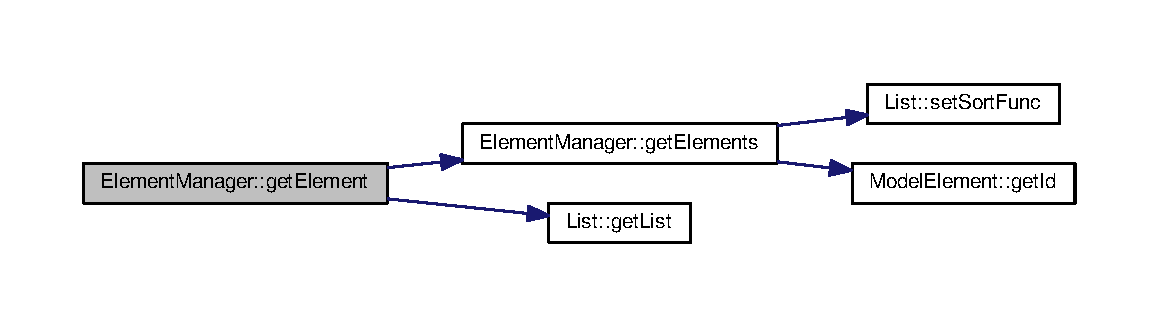
\includegraphics[width=350pt]{class_element_manager_a31be666a89f2a19583ac0bf3e124cf32_cgraph}
\end{center}
\end{figure}




Here is the caller graph for this function\+:\nopagebreak
\begin{figure}[H]
\begin{center}
\leavevmode
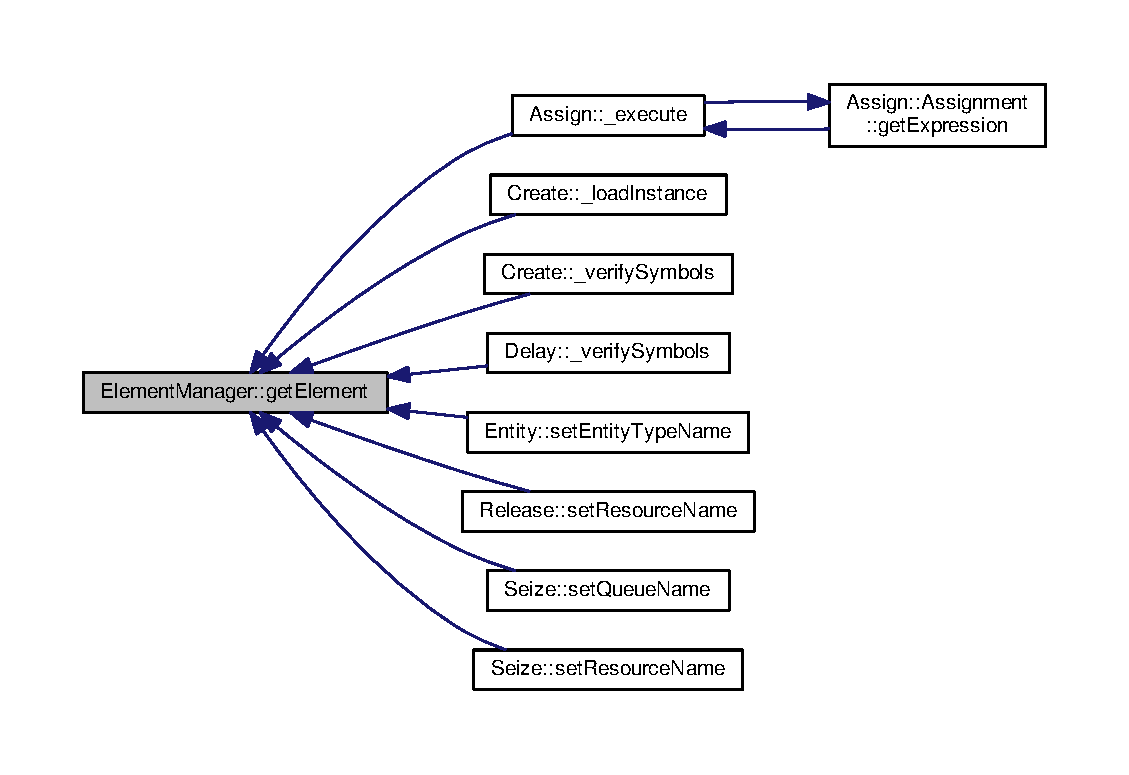
\includegraphics[width=350pt]{class_element_manager_a31be666a89f2a19583ac0bf3e124cf32_icgraph}
\end{center}
\end{figure}


\index{Element\+Manager@{Element\+Manager}!get\+Element@{get\+Element}}
\index{get\+Element@{get\+Element}!Element\+Manager@{Element\+Manager}}
\subsubsection[{\texorpdfstring{get\+Element(std\+::string infra\+Typename, std\+::string name)}{getElement(std::string infraTypename, std::string name)}}]{\setlength{\rightskip}{0pt plus 5cm}{\bf Model\+Element} $\ast$ Element\+Manager\+::get\+Element (
\begin{DoxyParamCaption}
\item[{std\+::string}]{infra\+Typename, }
\item[{std\+::string}]{name}
\end{DoxyParamCaption}
)}\hypertarget{class_element_manager_ae5f80eb977a94280705de474e49f2e04}{}\label{class_element_manager_ae5f80eb977a94280705de474e49f2e04}


Here is the call graph for this function\+:\nopagebreak
\begin{figure}[H]
\begin{center}
\leavevmode
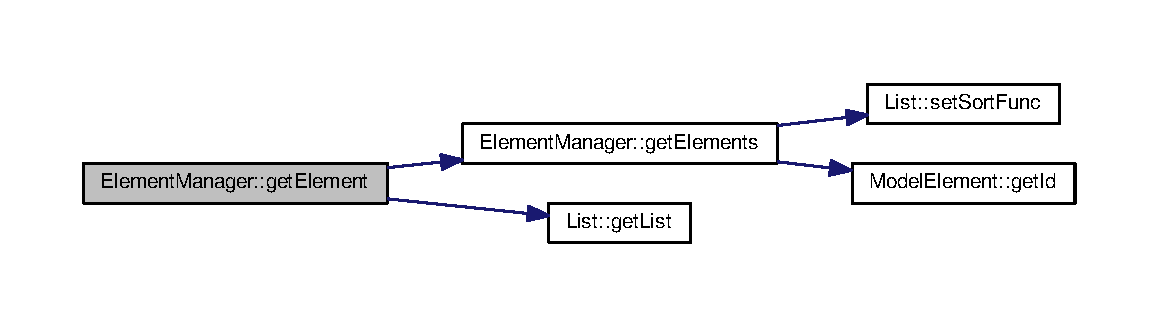
\includegraphics[width=350pt]{class_element_manager_ae5f80eb977a94280705de474e49f2e04_cgraph}
\end{center}
\end{figure}


\index{Element\+Manager@{Element\+Manager}!get\+Elements@{get\+Elements}}
\index{get\+Elements@{get\+Elements}!Element\+Manager@{Element\+Manager}}
\subsubsection[{\texorpdfstring{get\+Elements(std\+::string infra\+Typename) const }{getElements(std::string infraTypename) const }}]{\setlength{\rightskip}{0pt plus 5cm}{\bf List}$<$ {\bf Model\+Element} $\ast$ $>$ $\ast$ Element\+Manager\+::get\+Elements (
\begin{DoxyParamCaption}
\item[{std\+::string}]{infra\+Typename}
\end{DoxyParamCaption}
) const}\hypertarget{class_element_manager_a1c2f03e1279b3f2686e21f670edb1173}{}\label{class_element_manager_a1c2f03e1279b3f2686e21f670edb1173}


Here is the call graph for this function\+:\nopagebreak
\begin{figure}[H]
\begin{center}
\leavevmode
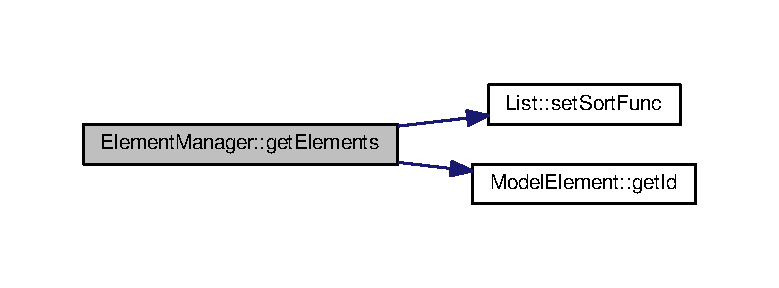
\includegraphics[width=350pt]{class_element_manager_a1c2f03e1279b3f2686e21f670edb1173_cgraph}
\end{center}
\end{figure}




Here is the caller graph for this function\+:\nopagebreak
\begin{figure}[H]
\begin{center}
\leavevmode
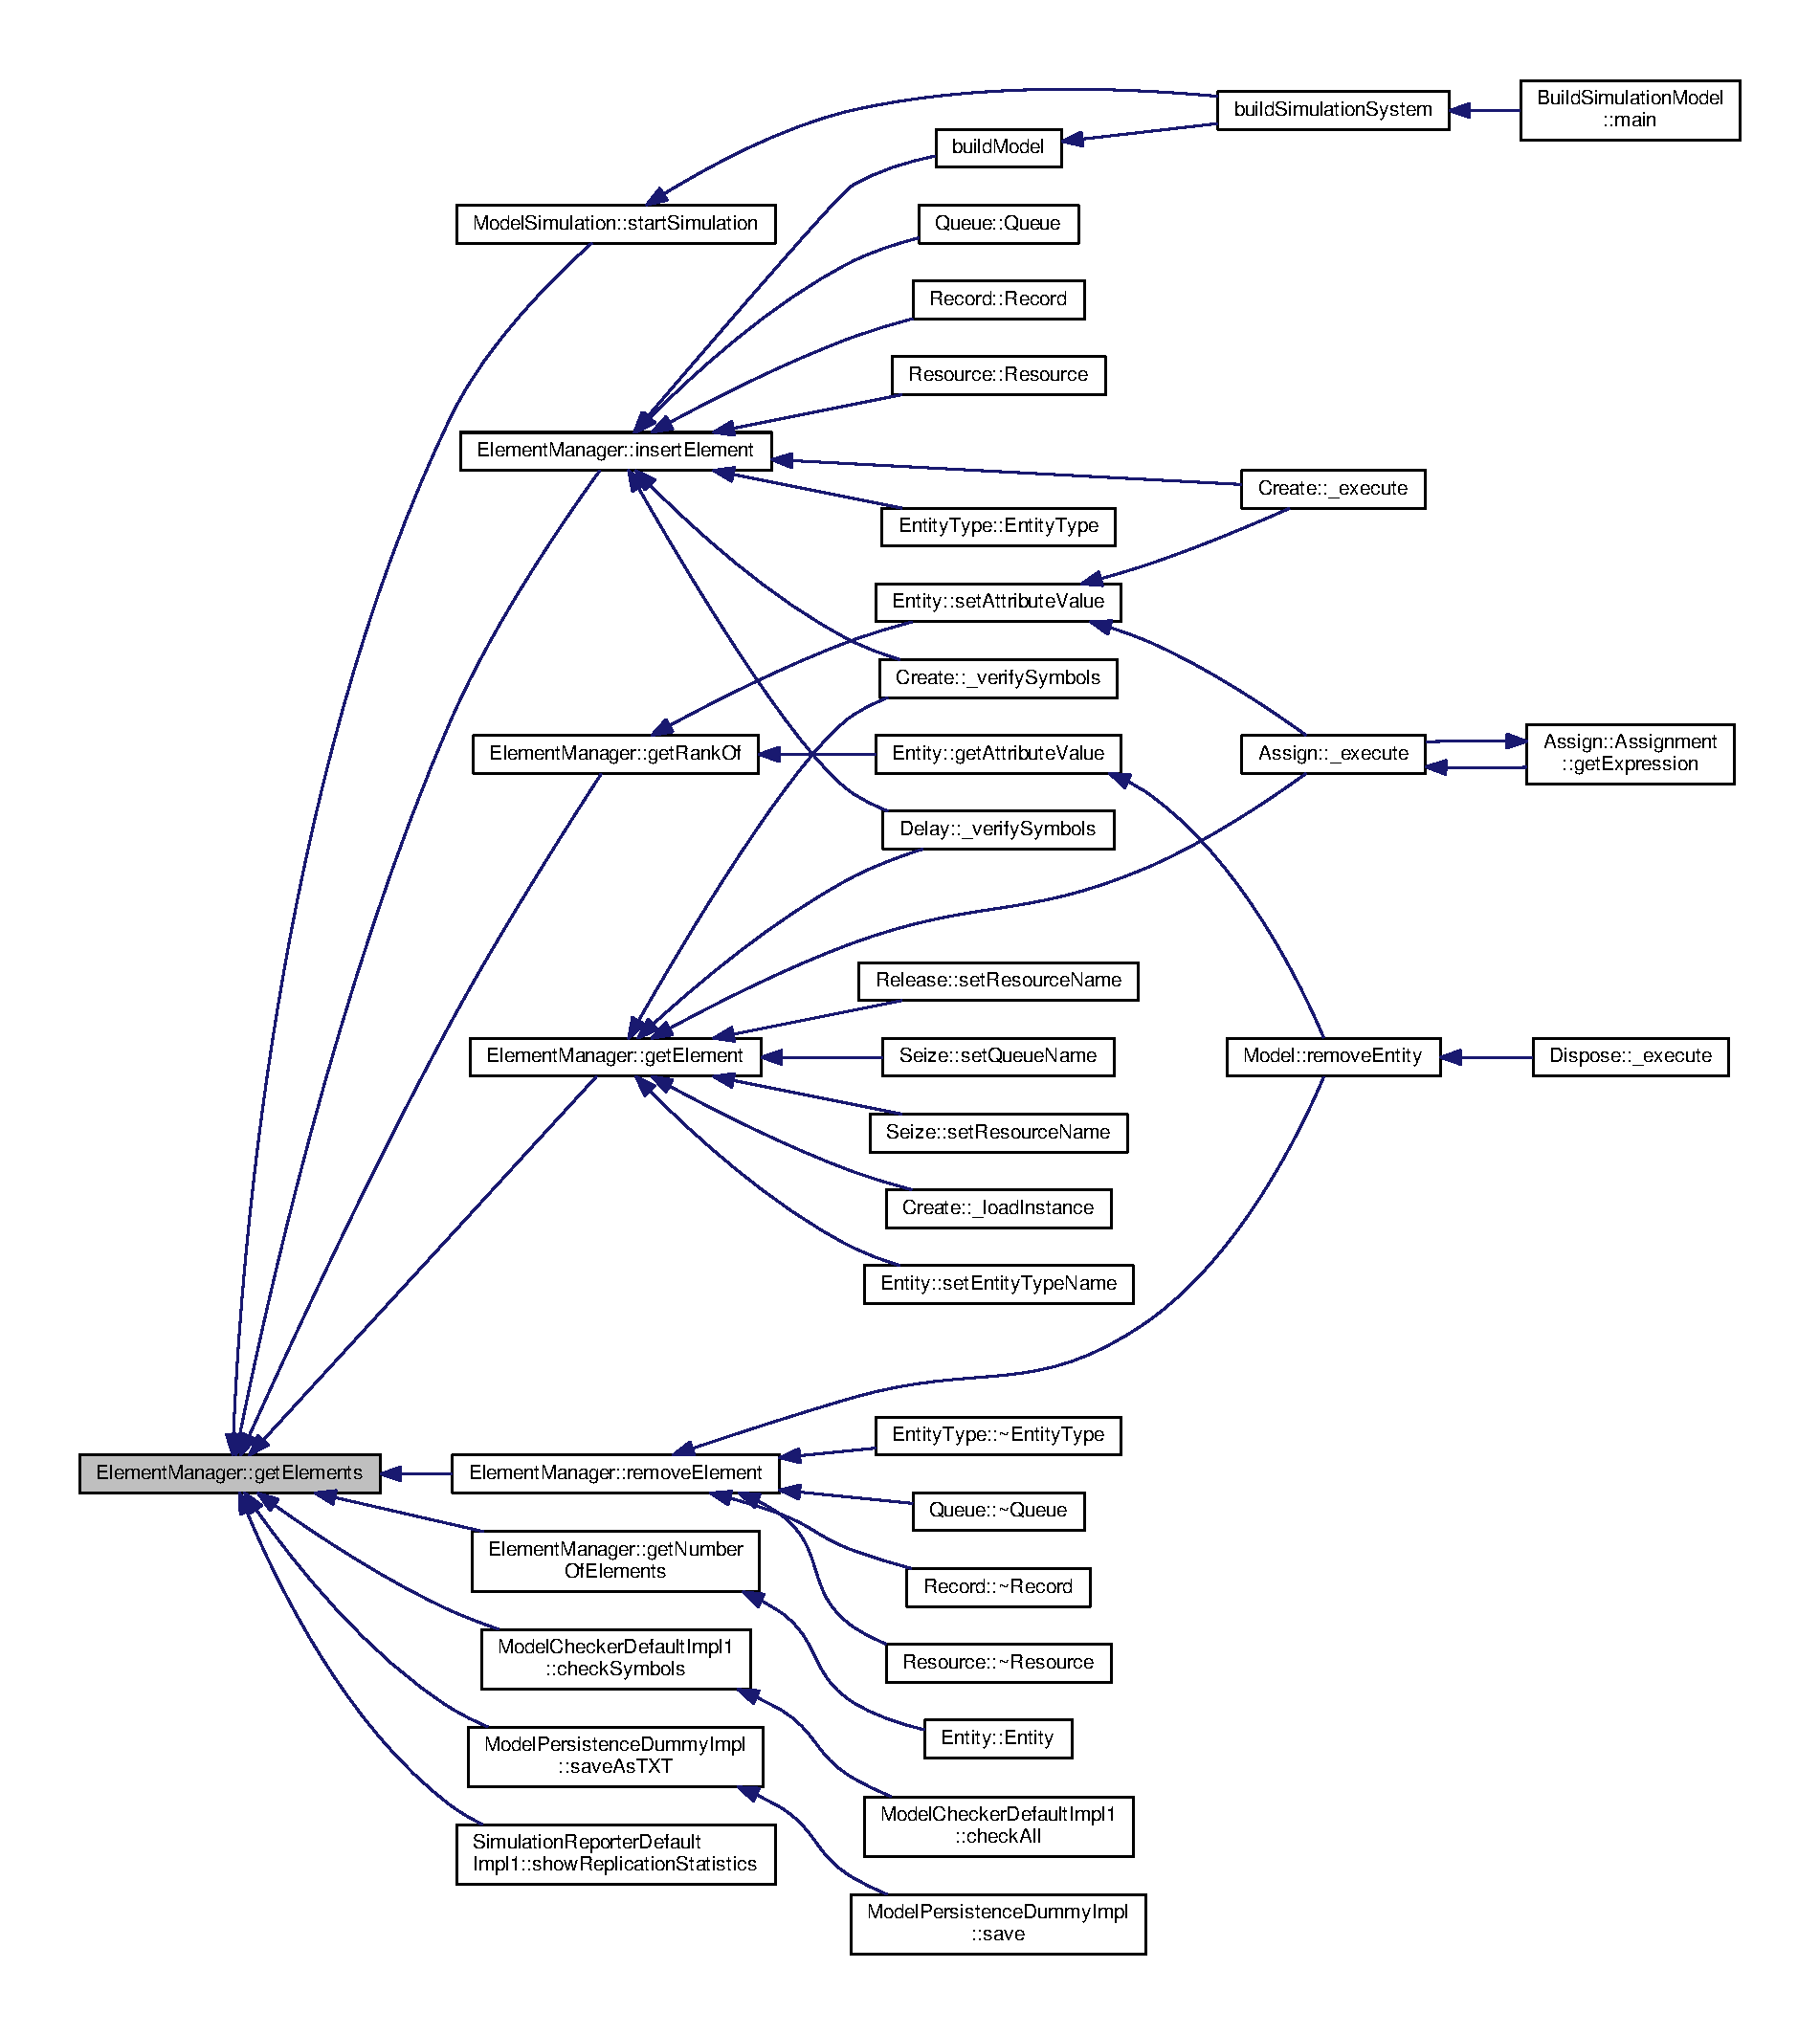
\includegraphics[width=350pt]{class_element_manager_a1c2f03e1279b3f2686e21f670edb1173_icgraph}
\end{center}
\end{figure}


\index{Element\+Manager@{Element\+Manager}!get\+Element\+Typenames@{get\+Element\+Typenames}}
\index{get\+Element\+Typenames@{get\+Element\+Typenames}!Element\+Manager@{Element\+Manager}}
\subsubsection[{\texorpdfstring{get\+Element\+Typenames() const }{getElementTypenames() const }}]{\setlength{\rightskip}{0pt plus 5cm}std\+::list$<$ std\+::string $>$ $\ast$ Element\+Manager\+::get\+Element\+Typenames (
\begin{DoxyParamCaption}
{}
\end{DoxyParamCaption}
) const}\hypertarget{class_element_manager_a58c8c572a76a712c3da42baafa888a8a}{}\label{class_element_manager_a58c8c572a76a712c3da42baafa888a8a}


Here is the caller graph for this function\+:\nopagebreak
\begin{figure}[H]
\begin{center}
\leavevmode
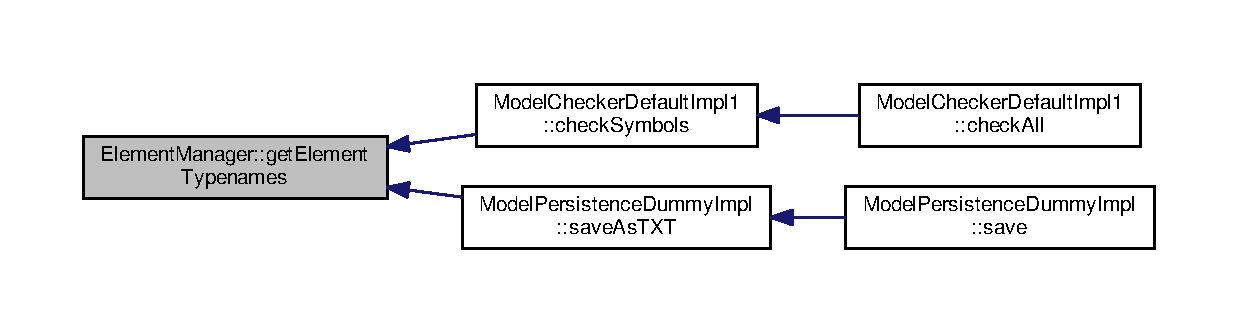
\includegraphics[width=350pt]{class_element_manager_a58c8c572a76a712c3da42baafa888a8a_icgraph}
\end{center}
\end{figure}


\index{Element\+Manager@{Element\+Manager}!get\+Number\+Of\+Elements@{get\+Number\+Of\+Elements}}
\index{get\+Number\+Of\+Elements@{get\+Number\+Of\+Elements}!Element\+Manager@{Element\+Manager}}
\subsubsection[{\texorpdfstring{get\+Number\+Of\+Elements(std\+::string infra\+Typename)}{getNumberOfElements(std::string infraTypename)}}]{\setlength{\rightskip}{0pt plus 5cm}unsigned int Element\+Manager\+::get\+Number\+Of\+Elements (
\begin{DoxyParamCaption}
\item[{std\+::string}]{infra\+Typename}
\end{DoxyParamCaption}
)}\hypertarget{class_element_manager_ade38f33e0b0902ea4d4e756592c77998}{}\label{class_element_manager_ade38f33e0b0902ea4d4e756592c77998}


Here is the call graph for this function\+:\nopagebreak
\begin{figure}[H]
\begin{center}
\leavevmode
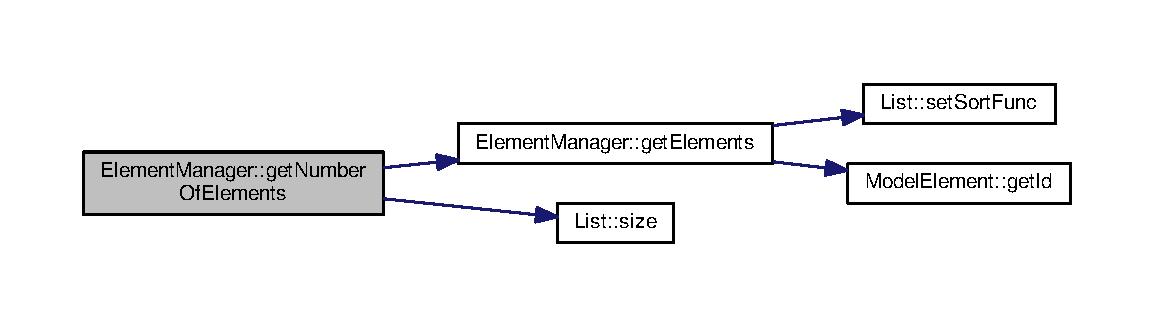
\includegraphics[width=350pt]{class_element_manager_ade38f33e0b0902ea4d4e756592c77998_cgraph}
\end{center}
\end{figure}




Here is the caller graph for this function\+:\nopagebreak
\begin{figure}[H]
\begin{center}
\leavevmode
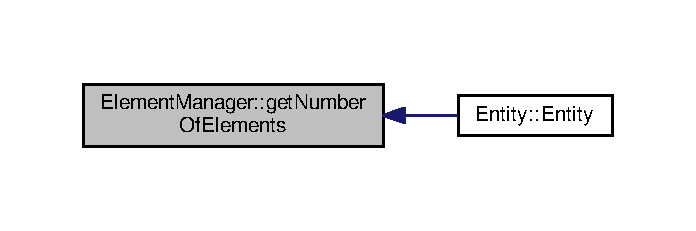
\includegraphics[width=334pt]{class_element_manager_ade38f33e0b0902ea4d4e756592c77998_icgraph}
\end{center}
\end{figure}


\index{Element\+Manager@{Element\+Manager}!get\+Rank\+Of@{get\+Rank\+Of}}
\index{get\+Rank\+Of@{get\+Rank\+Of}!Element\+Manager@{Element\+Manager}}
\subsubsection[{\texorpdfstring{get\+Rank\+Of(std\+::string infra\+Typename, std\+::string name)}{getRankOf(std::string infraTypename, std::string name)}}]{\setlength{\rightskip}{0pt plus 5cm}int Element\+Manager\+::get\+Rank\+Of (
\begin{DoxyParamCaption}
\item[{std\+::string}]{infra\+Typename, }
\item[{std\+::string}]{name}
\end{DoxyParamCaption}
)}\hypertarget{class_element_manager_a9d3f036b85665023061f62c19cdf0cc0}{}\label{class_element_manager_a9d3f036b85665023061f62c19cdf0cc0}


returns the position (1st position=0) of the element if found, or negative value if not found 



Here is the call graph for this function\+:\nopagebreak
\begin{figure}[H]
\begin{center}
\leavevmode
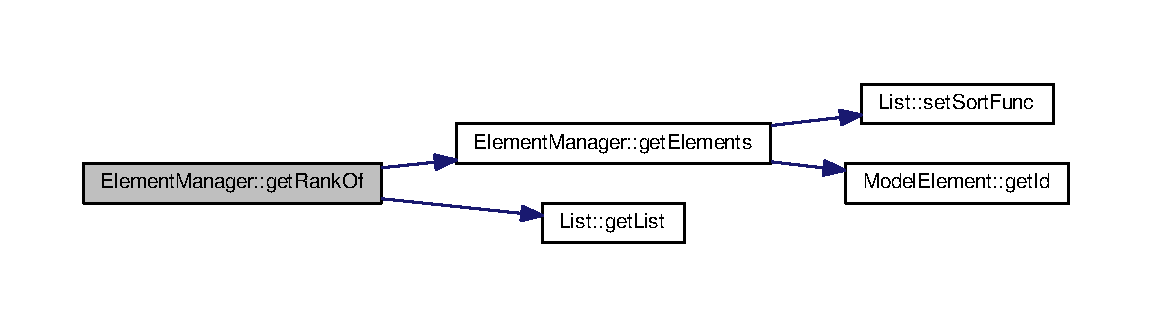
\includegraphics[width=350pt]{class_element_manager_a9d3f036b85665023061f62c19cdf0cc0_cgraph}
\end{center}
\end{figure}




Here is the caller graph for this function\+:\nopagebreak
\begin{figure}[H]
\begin{center}
\leavevmode
\includegraphics[width=350pt]{class_element_manager_a9d3f036b85665023061f62c19cdf0cc0_icgraph}
\end{center}
\end{figure}


\index{Element\+Manager@{Element\+Manager}!insert\+Element@{insert\+Element}}
\index{insert\+Element@{insert\+Element}!Element\+Manager@{Element\+Manager}}
\subsubsection[{\texorpdfstring{insert\+Element(std\+::string infra\+Typename, Model\+Element $\ast$infra)}{insertElement(std::string infraTypename, ModelElement *infra)}}]{\setlength{\rightskip}{0pt plus 5cm}bool Element\+Manager\+::insert\+Element (
\begin{DoxyParamCaption}
\item[{std\+::string}]{infra\+Typename, }
\item[{{\bf Model\+Element} $\ast$}]{infra}
\end{DoxyParamCaption}
)}\hypertarget{class_element_manager_ad3158696ee88632fe42e5cebb2af4582}{}\label{class_element_manager_ad3158696ee88632fe42e5cebb2af4582}


Here is the call graph for this function\+:\nopagebreak
\begin{figure}[H]
\begin{center}
\leavevmode
\includegraphics[width=350pt]{class_element_manager_ad3158696ee88632fe42e5cebb2af4582_cgraph}
\end{center}
\end{figure}




Here is the caller graph for this function\+:\nopagebreak
\begin{figure}[H]
\begin{center}
\leavevmode
\includegraphics[width=350pt]{class_element_manager_ad3158696ee88632fe42e5cebb2af4582_icgraph}
\end{center}
\end{figure}


\index{Element\+Manager@{Element\+Manager}!remove\+Element@{remove\+Element}}
\index{remove\+Element@{remove\+Element}!Element\+Manager@{Element\+Manager}}
\subsubsection[{\texorpdfstring{remove\+Element(std\+::string infra\+Typename, Model\+Element $\ast$infra)}{removeElement(std::string infraTypename, ModelElement *infra)}}]{\setlength{\rightskip}{0pt plus 5cm}void Element\+Manager\+::remove\+Element (
\begin{DoxyParamCaption}
\item[{std\+::string}]{infra\+Typename, }
\item[{{\bf Model\+Element} $\ast$}]{infra}
\end{DoxyParamCaption}
)}\hypertarget{class_element_manager_a2f918ec41d81e4ec0ba14fa6c6ab249a}{}\label{class_element_manager_a2f918ec41d81e4ec0ba14fa6c6ab249a}


Here is the call graph for this function\+:\nopagebreak
\begin{figure}[H]
\begin{center}
\leavevmode
\includegraphics[width=350pt]{class_element_manager_a2f918ec41d81e4ec0ba14fa6c6ab249a_cgraph}
\end{center}
\end{figure}




Here is the caller graph for this function\+:\nopagebreak
\begin{figure}[H]
\begin{center}
\leavevmode
\includegraphics[width=350pt]{class_element_manager_a2f918ec41d81e4ec0ba14fa6c6ab249a_icgraph}
\end{center}
\end{figure}


\index{Element\+Manager@{Element\+Manager}!show@{show}}
\index{show@{show}!Element\+Manager@{Element\+Manager}}
\subsubsection[{\texorpdfstring{show()}{show()}}]{\setlength{\rightskip}{0pt plus 5cm}void Element\+Manager\+::show (
\begin{DoxyParamCaption}
{}
\end{DoxyParamCaption}
)}\hypertarget{class_element_manager_a77b13541fb1da854d2680802778b5a64}{}\label{class_element_manager_a77b13541fb1da854d2680802778b5a64}


Here is the call graph for this function\+:\nopagebreak
\begin{figure}[H]
\begin{center}
\leavevmode
\includegraphics[width=350pt]{class_element_manager_a77b13541fb1da854d2680802778b5a64_cgraph}
\end{center}
\end{figure}




The documentation for this class was generated from the following files\+:\begin{DoxyCompactItemize}
\item 
\hyperlink{_element_manager_8h}{Element\+Manager.\+h}\item 
\hyperlink{_element_manager_8cpp}{Element\+Manager.\+cpp}\end{DoxyCompactItemize}

\hypertarget{class_element_manager__if}{}\section{Element\+Manager\+\_\+if Class Reference}
\label{class_element_manager__if}\index{Element\+Manager\+\_\+if@{Element\+Manager\+\_\+if}}


{\ttfamily \#include $<$Element\+Manager\+\_\+if.\+h$>$}

\subsection*{Public Member Functions}
\begin{DoxyCompactItemize}
\item 
\hyperlink{class_element_manager__if_a036a154585b5d10a37c2ce6381566f6e}{Element\+Manager\+\_\+if} ()
\item 
\hyperlink{class_element_manager__if_aab59380713d6f411cf397a38f6e2aad3}{Element\+Manager\+\_\+if} (const \hyperlink{class_element_manager__if}{Element\+Manager\+\_\+if} \&orig)
\item 
virtual \hyperlink{class_element_manager__if_a10ee01eb7b5b5ef3232eb39677e4ddcb}{$\sim$\+Element\+Manager\+\_\+if} ()
\end{DoxyCompactItemize}


\subsection{Constructor \& Destructor Documentation}
\index{Element\+Manager\+\_\+if@{Element\+Manager\+\_\+if}!Element\+Manager\+\_\+if@{Element\+Manager\+\_\+if}}
\index{Element\+Manager\+\_\+if@{Element\+Manager\+\_\+if}!Element\+Manager\+\_\+if@{Element\+Manager\+\_\+if}}
\subsubsection[{\texorpdfstring{Element\+Manager\+\_\+if()}{ElementManager_if()}}]{\setlength{\rightskip}{0pt plus 5cm}Element\+Manager\+\_\+if\+::\+Element\+Manager\+\_\+if (
\begin{DoxyParamCaption}
{}
\end{DoxyParamCaption}
)}\hypertarget{class_element_manager__if_a036a154585b5d10a37c2ce6381566f6e}{}\label{class_element_manager__if_a036a154585b5d10a37c2ce6381566f6e}
\index{Element\+Manager\+\_\+if@{Element\+Manager\+\_\+if}!Element\+Manager\+\_\+if@{Element\+Manager\+\_\+if}}
\index{Element\+Manager\+\_\+if@{Element\+Manager\+\_\+if}!Element\+Manager\+\_\+if@{Element\+Manager\+\_\+if}}
\subsubsection[{\texorpdfstring{Element\+Manager\+\_\+if(const Element\+Manager\+\_\+if \&orig)}{ElementManager_if(const ElementManager_if &orig)}}]{\setlength{\rightskip}{0pt plus 5cm}Element\+Manager\+\_\+if\+::\+Element\+Manager\+\_\+if (
\begin{DoxyParamCaption}
\item[{const {\bf Element\+Manager\+\_\+if} \&}]{orig}
\end{DoxyParamCaption}
)}\hypertarget{class_element_manager__if_aab59380713d6f411cf397a38f6e2aad3}{}\label{class_element_manager__if_aab59380713d6f411cf397a38f6e2aad3}
\index{Element\+Manager\+\_\+if@{Element\+Manager\+\_\+if}!````~Element\+Manager\+\_\+if@{$\sim$\+Element\+Manager\+\_\+if}}
\index{````~Element\+Manager\+\_\+if@{$\sim$\+Element\+Manager\+\_\+if}!Element\+Manager\+\_\+if@{Element\+Manager\+\_\+if}}
\subsubsection[{\texorpdfstring{$\sim$\+Element\+Manager\+\_\+if()}{~ElementManager_if()}}]{\setlength{\rightskip}{0pt plus 5cm}virtual Element\+Manager\+\_\+if\+::$\sim$\+Element\+Manager\+\_\+if (
\begin{DoxyParamCaption}
{}
\end{DoxyParamCaption}
)\hspace{0.3cm}{\ttfamily [virtual]}}\hypertarget{class_element_manager__if_a10ee01eb7b5b5ef3232eb39677e4ddcb}{}\label{class_element_manager__if_a10ee01eb7b5b5ef3232eb39677e4ddcb}


The documentation for this class was generated from the following file\+:\begin{DoxyCompactItemize}
\item 
\hyperlink{_element_manager__if_8h}{Element\+Manager\+\_\+if.\+h}\end{DoxyCompactItemize}

\hypertarget{class_entity}{\section{Entity Class Reference}
\label{class_entity}\index{Entity@{Entity}}
}


{\ttfamily \#include $<$Entity.\-h$>$}



Inheritance diagram for Entity\-:\nopagebreak
\begin{figure}[H]
\begin{center}
\leavevmode
\includegraphics[width=180pt]{class_entity__inherit__graph}
\end{center}
\end{figure}


Collaboration diagram for Entity\-:\nopagebreak
\begin{figure}[H]
\begin{center}
\leavevmode
\includegraphics[width=180pt]{class_entity__coll__graph}
\end{center}
\end{figure}
\subsection*{Public Member Functions}
\begin{DoxyCompactItemize}
\item 
\hyperlink{class_entity_a980f368aa07ce358583982821533a54a}{Entity} ()
\item 
\hyperlink{class_entity_a9de139ff12775dd95fb80bec08247de7}{Entity} (const \hyperlink{class_entity}{Entity} \&orig)
\item 
virtual \hyperlink{class_entity_adf6d3f7cb1b2ba029b6b048a395cc8ae}{$\sim$\-Entity} ()
\item 
virtual std\-::string \hyperlink{class_entity_a86cc324050b451b31b134943e7978e36}{show} ()
\item 
std\-::map$<$ std\-::string, \\*
\hyperlink{class_attribute_value}{Attribute\-Value} $\ast$ $>$ $\ast$ \hyperlink{class_entity_a5990dbefc2f21a7e8e0f91f9bf434fb9}{get\-Attribute\-Values} () const 
\item 
void \hyperlink{class_entity_a40053760a2c84dd72fd5aeb425f6781d}{set\-Entity\-Type\-Name} (std\-::string \-\_\-entity\-Type\-Name)
\item 
std\-::string \hyperlink{class_entity_a860a6385aa2af6b8d205a8e3ea912c38}{get\-Entity\-Type\-Name} () const 
\end{DoxyCompactItemize}
\subsection*{Additional Inherited Members}


\subsection{Constructor \& Destructor Documentation}
\hypertarget{class_entity_a980f368aa07ce358583982821533a54a}{\index{Entity@{Entity}!Entity@{Entity}}
\index{Entity@{Entity}!Entity@{Entity}}
\subsubsection[{Entity}]{\setlength{\rightskip}{0pt plus 5cm}Entity\-::\-Entity (
\begin{DoxyParamCaption}
{}
\end{DoxyParamCaption}
)}}\label{class_entity_a980f368aa07ce358583982821533a54a}
\hypertarget{class_entity_a9de139ff12775dd95fb80bec08247de7}{\index{Entity@{Entity}!Entity@{Entity}}
\index{Entity@{Entity}!Entity@{Entity}}
\subsubsection[{Entity}]{\setlength{\rightskip}{0pt plus 5cm}Entity\-::\-Entity (
\begin{DoxyParamCaption}
\item[{const {\bf Entity} \&}]{orig}
\end{DoxyParamCaption}
)}}\label{class_entity_a9de139ff12775dd95fb80bec08247de7}
\hypertarget{class_entity_adf6d3f7cb1b2ba029b6b048a395cc8ae}{\index{Entity@{Entity}!$\sim$\-Entity@{$\sim$\-Entity}}
\index{$\sim$\-Entity@{$\sim$\-Entity}!Entity@{Entity}}
\subsubsection[{$\sim$\-Entity}]{\setlength{\rightskip}{0pt plus 5cm}Entity\-::$\sim$\-Entity (
\begin{DoxyParamCaption}
{}
\end{DoxyParamCaption}
)\hspace{0.3cm}{\ttfamily [virtual]}}}\label{class_entity_adf6d3f7cb1b2ba029b6b048a395cc8ae}


\subsection{Member Function Documentation}
\hypertarget{class_entity_a5990dbefc2f21a7e8e0f91f9bf434fb9}{\index{Entity@{Entity}!get\-Attribute\-Values@{get\-Attribute\-Values}}
\index{get\-Attribute\-Values@{get\-Attribute\-Values}!Entity@{Entity}}
\subsubsection[{get\-Attribute\-Values}]{\setlength{\rightskip}{0pt plus 5cm}std\-::map$<$ std\-::string, {\bf Attribute\-Value} $\ast$ $>$ $\ast$ Entity\-::get\-Attribute\-Values (
\begin{DoxyParamCaption}
{}
\end{DoxyParamCaption}
) const}}\label{class_entity_a5990dbefc2f21a7e8e0f91f9bf434fb9}
\hypertarget{class_entity_a860a6385aa2af6b8d205a8e3ea912c38}{\index{Entity@{Entity}!get\-Entity\-Type\-Name@{get\-Entity\-Type\-Name}}
\index{get\-Entity\-Type\-Name@{get\-Entity\-Type\-Name}!Entity@{Entity}}
\subsubsection[{get\-Entity\-Type\-Name}]{\setlength{\rightskip}{0pt plus 5cm}std\-::string Entity\-::get\-Entity\-Type\-Name (
\begin{DoxyParamCaption}
{}
\end{DoxyParamCaption}
) const}}\label{class_entity_a860a6385aa2af6b8d205a8e3ea912c38}
\hypertarget{class_entity_a40053760a2c84dd72fd5aeb425f6781d}{\index{Entity@{Entity}!set\-Entity\-Type\-Name@{set\-Entity\-Type\-Name}}
\index{set\-Entity\-Type\-Name@{set\-Entity\-Type\-Name}!Entity@{Entity}}
\subsubsection[{set\-Entity\-Type\-Name}]{\setlength{\rightskip}{0pt plus 5cm}void Entity\-::set\-Entity\-Type\-Name (
\begin{DoxyParamCaption}
\item[{std\-::string}]{\-\_\-entity\-Type\-Name}
\end{DoxyParamCaption}
)}}\label{class_entity_a40053760a2c84dd72fd5aeb425f6781d}
\hypertarget{class_entity_a86cc324050b451b31b134943e7978e36}{\index{Entity@{Entity}!show@{show}}
\index{show@{show}!Entity@{Entity}}
\subsubsection[{show}]{\setlength{\rightskip}{0pt plus 5cm}std\-::string Entity\-::show (
\begin{DoxyParamCaption}
{}
\end{DoxyParamCaption}
)\hspace{0.3cm}{\ttfamily [virtual]}}}\label{class_entity_a86cc324050b451b31b134943e7978e36}


Reimplemented from \hyperlink{class_model_infrastructure_a649a5a89a0c9931783d3c51de2acf266}{Model\-Infrastructure}.



Here is the call graph for this function\-:\nopagebreak
\begin{figure}[H]
\begin{center}
\leavevmode
\includegraphics[width=290pt]{class_entity_a86cc324050b451b31b134943e7978e36_cgraph}
\end{center}
\end{figure}




The documentation for this class was generated from the following files\-:\begin{DoxyCompactItemize}
\item 
\hyperlink{_entity_8h}{Entity.\-h}\item 
\hyperlink{_entity_8cpp}{Entity.\-cpp}\end{DoxyCompactItemize}

\hypertarget{class_entity_type}{\section{Entity\-Type Class Reference}
\label{class_entity_type}\index{Entity\-Type@{Entity\-Type}}
}


{\ttfamily \#include $<$Entity\-Type.\-h$>$}



Inheritance diagram for Entity\-Type\-:\nopagebreak
\begin{figure}[H]
\begin{center}
\leavevmode
\includegraphics[width=180pt]{class_entity_type__inherit__graph}
\end{center}
\end{figure}


Collaboration diagram for Entity\-Type\-:\nopagebreak
\begin{figure}[H]
\begin{center}
\leavevmode
\includegraphics[width=180pt]{class_entity_type__coll__graph}
\end{center}
\end{figure}
\subsection*{Public Member Functions}
\begin{DoxyCompactItemize}
\item 
\hyperlink{class_entity_type_a76c09c732793a586dc3b474485e9824f}{Entity\-Type} (\hyperlink{class_model}{Model} $\ast$model)
\item 
\hyperlink{class_entity_type_a34b9576e2453ed309c75840319bbb2f8}{Entity\-Type} (const \hyperlink{class_entity_type}{Entity\-Type} \&orig)
\item 
virtual \hyperlink{class_entity_type_aee11e4242d000965f06018723bdf0946}{$\sim$\-Entity\-Type} ()
\item 
virtual std\-::string \hyperlink{class_entity_type_ab5a696912b12a9f51decded90f368dea}{show} ()
\item 
void \hyperlink{class_entity_type_affd1d2dd13149ae0989aae5cc9ea1e05}{set\-Initial\-Waiting\-Cost} (double \-\_\-initial\-Waiting\-Cost)
\item 
double \hyperlink{class_entity_type_a46dd0977b19bf167eeb12db97464b757}{get\-Initial\-Waiting\-Cost} () const 
\item 
void \hyperlink{class_entity_type_a32f126822c567a887a446a763db13d64}{set\-Initial\-Other\-Cost} (double \-\_\-initial\-Other\-Cost)
\item 
double \hyperlink{class_entity_type_ac5708811f5f6eaf7ac587fc88190b7f2}{get\-Initial\-Other\-Cost} () const 
\item 
void \hyperlink{class_entity_type_a935cac67adc2b13aa25290c3db04c847}{set\-Initial\-N\-V\-A\-Cost} (double \-\_\-initial\-N\-V\-A\-Cost)
\item 
double \hyperlink{class_entity_type_ae8b26deba82e687d5a07b863f750baf4}{get\-Initial\-N\-V\-A\-Cost} () const 
\item 
void \hyperlink{class_entity_type_aecd52de7178bb03be55798378d15d3e8}{set\-Initial\-V\-A\-Cost} (double \-\_\-initial\-V\-A\-Cost)
\item 
double \hyperlink{class_entity_type_a9833d4a85dcb5c5bd9db02e1e2e45dd9}{get\-Initial\-V\-A\-Cost} () const 
\item 
void \hyperlink{class_entity_type_ab3a19031f9b46b376bdd35aa3044c90e}{set\-Initial\-Picture} (std\-::string \-\_\-initial\-Picture)
\item 
std\-::string \hyperlink{class_entity_type_a9a464c546bc2f7fe56fbea9b761ac1f7}{get\-Initial\-Picture} () const 
\item 
\hyperlink{class_statistics_collector}{Statistics\-Collector} $\ast$ \hyperlink{class_entity_type_acdcb00168a8fc2e23cf8bf3302464ce3}{get\-Cstat\-Time\-In\-System} () const 
\item 
\hyperlink{class_statistics_collector}{Statistics\-Collector} $\ast$ \hyperlink{class_entity_type_a48e1dedd3e7d7b198ee4e7a61c6afb7e}{get\-Cstat\-N\-V\-A\-Time} () const 
\item 
\hyperlink{class_statistics_collector}{Statistics\-Collector} $\ast$ \hyperlink{class_entity_type_aafb65d3cdceae776da454989b7b4a874}{get\-Cstat\-V\-A\-Time} () const 
\item 
\hyperlink{class_statistics_collector}{Statistics\-Collector} $\ast$ \hyperlink{class_entity_type_a8b6a8b11d428c9e23800d01701e7fbd1}{get\-Cstat\-Other\-Time} () const 
\item 
\hyperlink{class_statistics_collector}{Statistics\-Collector} $\ast$ \hyperlink{class_entity_type_a2604288226dd7fc0c6c322d415b891cc}{get\-Cstat\-Transfer\-Time} () const 
\item 
\hyperlink{class_statistics_collector}{Statistics\-Collector} $\ast$ \hyperlink{class_entity_type_ae43feed54cd8661efb317ef4891bcfcf}{get\-Cstat\-Waiting\-Time} () const 
\end{DoxyCompactItemize}
\subsection*{Protected Member Functions}
\begin{DoxyCompactItemize}
\item 
virtual void \hyperlink{class_entity_type_af88c3d67f9eb8b92b4e32e04bed6730f}{\-\_\-load\-Instance} (std\-::list$<$ std\-::string $>$ words)
\item 
virtual std\-::list$<$ std\-::string $>$ $\ast$ \hyperlink{class_entity_type_a4f6179d5043e750d9555d6eeef8de4cd}{\-\_\-save\-Instance} ()
\item 
virtual bool \hyperlink{class_entity_type_a50e21c4807823132e777529c70bf7cef}{\-\_\-verify\-Symbols} (std\-::string $\ast$error\-Message)
\end{DoxyCompactItemize}
\subsection*{Additional Inherited Members}


\subsection{Detailed Description}


Definition at line 22 of file Entity\-Type.\-h.



\subsection{Constructor \& Destructor Documentation}
\hypertarget{class_entity_type_a76c09c732793a586dc3b474485e9824f}{\index{Entity\-Type@{Entity\-Type}!Entity\-Type@{Entity\-Type}}
\index{Entity\-Type@{Entity\-Type}!EntityType@{Entity\-Type}}
\subsubsection[{Entity\-Type}]{\setlength{\rightskip}{0pt plus 5cm}Entity\-Type\-::\-Entity\-Type (
\begin{DoxyParamCaption}
\item[{{\bf Model} $\ast$}]{model}
\end{DoxyParamCaption}
)}}\label{class_entity_type_a76c09c732793a586dc3b474485e9824f}


Definition at line 18 of file Entity\-Type.\-cpp.



Here is the call graph for this function\-:
\nopagebreak
\begin{figure}[H]
\begin{center}
\leavevmode
\includegraphics[width=350pt]{class_entity_type_a76c09c732793a586dc3b474485e9824f_cgraph}
\end{center}
\end{figure}


\hypertarget{class_entity_type_a34b9576e2453ed309c75840319bbb2f8}{\index{Entity\-Type@{Entity\-Type}!Entity\-Type@{Entity\-Type}}
\index{Entity\-Type@{Entity\-Type}!EntityType@{Entity\-Type}}
\subsubsection[{Entity\-Type}]{\setlength{\rightskip}{0pt plus 5cm}Entity\-Type\-::\-Entity\-Type (
\begin{DoxyParamCaption}
\item[{const {\bf Entity\-Type} \&}]{orig}
\end{DoxyParamCaption}
)}}\label{class_entity_type_a34b9576e2453ed309c75840319bbb2f8}


Definition at line 29 of file Entity\-Type.\-cpp.

\hypertarget{class_entity_type_aee11e4242d000965f06018723bdf0946}{\index{Entity\-Type@{Entity\-Type}!$\sim$\-Entity\-Type@{$\sim$\-Entity\-Type}}
\index{$\sim$\-Entity\-Type@{$\sim$\-Entity\-Type}!EntityType@{Entity\-Type}}
\subsubsection[{$\sim$\-Entity\-Type}]{\setlength{\rightskip}{0pt plus 5cm}Entity\-Type\-::$\sim$\-Entity\-Type (
\begin{DoxyParamCaption}
{}
\end{DoxyParamCaption}
)\hspace{0.3cm}{\ttfamily [virtual]}}}\label{class_entity_type_aee11e4242d000965f06018723bdf0946}


Definition at line 32 of file Entity\-Type.\-cpp.



\subsection{Member Function Documentation}
\hypertarget{class_entity_type_af88c3d67f9eb8b92b4e32e04bed6730f}{\index{Entity\-Type@{Entity\-Type}!\-\_\-load\-Instance@{\-\_\-load\-Instance}}
\index{\-\_\-load\-Instance@{\-\_\-load\-Instance}!EntityType@{Entity\-Type}}
\subsubsection[{\-\_\-load\-Instance}]{\setlength{\rightskip}{0pt plus 5cm}void Entity\-Type\-::\-\_\-load\-Instance (
\begin{DoxyParamCaption}
\item[{std\-::list$<$ std\-::string $>$}]{words}
\end{DoxyParamCaption}
)\hspace{0.3cm}{\ttfamily [protected]}, {\ttfamily [virtual]}}}\label{class_entity_type_af88c3d67f9eb8b92b4e32e04bed6730f}


Implements \hyperlink{class_model_infrastructure_ae118c8ad2ac9d4397c40d004af51b2dc}{Model\-Infrastructure}.



Definition at line 104 of file Entity\-Type.\-cpp.

\hypertarget{class_entity_type_a4f6179d5043e750d9555d6eeef8de4cd}{\index{Entity\-Type@{Entity\-Type}!\-\_\-save\-Instance@{\-\_\-save\-Instance}}
\index{\-\_\-save\-Instance@{\-\_\-save\-Instance}!EntityType@{Entity\-Type}}
\subsubsection[{\-\_\-save\-Instance}]{\setlength{\rightskip}{0pt plus 5cm}std\-::list$<$ std\-::string $>$ $\ast$ Entity\-Type\-::\-\_\-save\-Instance (
\begin{DoxyParamCaption}
{}
\end{DoxyParamCaption}
)\hspace{0.3cm}{\ttfamily [protected]}, {\ttfamily [virtual]}}}\label{class_entity_type_a4f6179d5043e750d9555d6eeef8de4cd}


Implements \hyperlink{class_model_infrastructure_a3da2fd381c44752598bc448b207e8287}{Model\-Infrastructure}.



Definition at line 108 of file Entity\-Type.\-cpp.

\hypertarget{class_entity_type_a50e21c4807823132e777529c70bf7cef}{\index{Entity\-Type@{Entity\-Type}!\-\_\-verify\-Symbols@{\-\_\-verify\-Symbols}}
\index{\-\_\-verify\-Symbols@{\-\_\-verify\-Symbols}!EntityType@{Entity\-Type}}
\subsubsection[{\-\_\-verify\-Symbols}]{\setlength{\rightskip}{0pt plus 5cm}bool Entity\-Type\-::\-\_\-verify\-Symbols (
\begin{DoxyParamCaption}
\item[{std\-::string $\ast$}]{error\-Message}
\end{DoxyParamCaption}
)\hspace{0.3cm}{\ttfamily [protected]}, {\ttfamily [virtual]}}}\label{class_entity_type_a50e21c4807823132e777529c70bf7cef}


Implements \hyperlink{class_model_infrastructure_a43de089b35b96c32dd24ca4f9636a388}{Model\-Infrastructure}.



Definition at line 113 of file Entity\-Type.\-cpp.

\hypertarget{class_entity_type_a48e1dedd3e7d7b198ee4e7a61c6afb7e}{\index{Entity\-Type@{Entity\-Type}!get\-Cstat\-N\-V\-A\-Time@{get\-Cstat\-N\-V\-A\-Time}}
\index{get\-Cstat\-N\-V\-A\-Time@{get\-Cstat\-N\-V\-A\-Time}!EntityType@{Entity\-Type}}
\subsubsection[{get\-Cstat\-N\-V\-A\-Time}]{\setlength{\rightskip}{0pt plus 5cm}{\bf Statistics\-Collector} $\ast$ Entity\-Type\-::get\-Cstat\-N\-V\-A\-Time (
\begin{DoxyParamCaption}
{}
\end{DoxyParamCaption}
) const}}\label{class_entity_type_a48e1dedd3e7d7b198ee4e7a61c6afb7e}


Definition at line 84 of file Entity\-Type.\-cpp.

\hypertarget{class_entity_type_a8b6a8b11d428c9e23800d01701e7fbd1}{\index{Entity\-Type@{Entity\-Type}!get\-Cstat\-Other\-Time@{get\-Cstat\-Other\-Time}}
\index{get\-Cstat\-Other\-Time@{get\-Cstat\-Other\-Time}!EntityType@{Entity\-Type}}
\subsubsection[{get\-Cstat\-Other\-Time}]{\setlength{\rightskip}{0pt plus 5cm}{\bf Statistics\-Collector} $\ast$ Entity\-Type\-::get\-Cstat\-Other\-Time (
\begin{DoxyParamCaption}
{}
\end{DoxyParamCaption}
) const}}\label{class_entity_type_a8b6a8b11d428c9e23800d01701e7fbd1}


Definition at line 92 of file Entity\-Type.\-cpp.

\hypertarget{class_entity_type_acdcb00168a8fc2e23cf8bf3302464ce3}{\index{Entity\-Type@{Entity\-Type}!get\-Cstat\-Time\-In\-System@{get\-Cstat\-Time\-In\-System}}
\index{get\-Cstat\-Time\-In\-System@{get\-Cstat\-Time\-In\-System}!EntityType@{Entity\-Type}}
\subsubsection[{get\-Cstat\-Time\-In\-System}]{\setlength{\rightskip}{0pt plus 5cm}{\bf Statistics\-Collector} $\ast$ Entity\-Type\-::get\-Cstat\-Time\-In\-System (
\begin{DoxyParamCaption}
{}
\end{DoxyParamCaption}
) const}}\label{class_entity_type_acdcb00168a8fc2e23cf8bf3302464ce3}


Definition at line 80 of file Entity\-Type.\-cpp.

\hypertarget{class_entity_type_a2604288226dd7fc0c6c322d415b891cc}{\index{Entity\-Type@{Entity\-Type}!get\-Cstat\-Transfer\-Time@{get\-Cstat\-Transfer\-Time}}
\index{get\-Cstat\-Transfer\-Time@{get\-Cstat\-Transfer\-Time}!EntityType@{Entity\-Type}}
\subsubsection[{get\-Cstat\-Transfer\-Time}]{\setlength{\rightskip}{0pt plus 5cm}{\bf Statistics\-Collector} $\ast$ Entity\-Type\-::get\-Cstat\-Transfer\-Time (
\begin{DoxyParamCaption}
{}
\end{DoxyParamCaption}
) const}}\label{class_entity_type_a2604288226dd7fc0c6c322d415b891cc}


Definition at line 96 of file Entity\-Type.\-cpp.

\hypertarget{class_entity_type_aafb65d3cdceae776da454989b7b4a874}{\index{Entity\-Type@{Entity\-Type}!get\-Cstat\-V\-A\-Time@{get\-Cstat\-V\-A\-Time}}
\index{get\-Cstat\-V\-A\-Time@{get\-Cstat\-V\-A\-Time}!EntityType@{Entity\-Type}}
\subsubsection[{get\-Cstat\-V\-A\-Time}]{\setlength{\rightskip}{0pt plus 5cm}{\bf Statistics\-Collector} $\ast$ Entity\-Type\-::get\-Cstat\-V\-A\-Time (
\begin{DoxyParamCaption}
{}
\end{DoxyParamCaption}
) const}}\label{class_entity_type_aafb65d3cdceae776da454989b7b4a874}


Definition at line 88 of file Entity\-Type.\-cpp.

\hypertarget{class_entity_type_ae43feed54cd8661efb317ef4891bcfcf}{\index{Entity\-Type@{Entity\-Type}!get\-Cstat\-Waiting\-Time@{get\-Cstat\-Waiting\-Time}}
\index{get\-Cstat\-Waiting\-Time@{get\-Cstat\-Waiting\-Time}!EntityType@{Entity\-Type}}
\subsubsection[{get\-Cstat\-Waiting\-Time}]{\setlength{\rightskip}{0pt plus 5cm}{\bf Statistics\-Collector} $\ast$ Entity\-Type\-::get\-Cstat\-Waiting\-Time (
\begin{DoxyParamCaption}
{}
\end{DoxyParamCaption}
) const}}\label{class_entity_type_ae43feed54cd8661efb317ef4891bcfcf}


Definition at line 100 of file Entity\-Type.\-cpp.

\hypertarget{class_entity_type_ae8b26deba82e687d5a07b863f750baf4}{\index{Entity\-Type@{Entity\-Type}!get\-Initial\-N\-V\-A\-Cost@{get\-Initial\-N\-V\-A\-Cost}}
\index{get\-Initial\-N\-V\-A\-Cost@{get\-Initial\-N\-V\-A\-Cost}!EntityType@{Entity\-Type}}
\subsubsection[{get\-Initial\-N\-V\-A\-Cost}]{\setlength{\rightskip}{0pt plus 5cm}double Entity\-Type\-::get\-Initial\-N\-V\-A\-Cost (
\begin{DoxyParamCaption}
{}
\end{DoxyParamCaption}
) const}}\label{class_entity_type_ae8b26deba82e687d5a07b863f750baf4}


Definition at line 60 of file Entity\-Type.\-cpp.

\hypertarget{class_entity_type_ac5708811f5f6eaf7ac587fc88190b7f2}{\index{Entity\-Type@{Entity\-Type}!get\-Initial\-Other\-Cost@{get\-Initial\-Other\-Cost}}
\index{get\-Initial\-Other\-Cost@{get\-Initial\-Other\-Cost}!EntityType@{Entity\-Type}}
\subsubsection[{get\-Initial\-Other\-Cost}]{\setlength{\rightskip}{0pt plus 5cm}double Entity\-Type\-::get\-Initial\-Other\-Cost (
\begin{DoxyParamCaption}
{}
\end{DoxyParamCaption}
) const}}\label{class_entity_type_ac5708811f5f6eaf7ac587fc88190b7f2}


Definition at line 52 of file Entity\-Type.\-cpp.

\hypertarget{class_entity_type_a9a464c546bc2f7fe56fbea9b761ac1f7}{\index{Entity\-Type@{Entity\-Type}!get\-Initial\-Picture@{get\-Initial\-Picture}}
\index{get\-Initial\-Picture@{get\-Initial\-Picture}!EntityType@{Entity\-Type}}
\subsubsection[{get\-Initial\-Picture}]{\setlength{\rightskip}{0pt plus 5cm}std\-::string Entity\-Type\-::get\-Initial\-Picture (
\begin{DoxyParamCaption}
{}
\end{DoxyParamCaption}
) const}}\label{class_entity_type_a9a464c546bc2f7fe56fbea9b761ac1f7}


Definition at line 76 of file Entity\-Type.\-cpp.

\hypertarget{class_entity_type_a9833d4a85dcb5c5bd9db02e1e2e45dd9}{\index{Entity\-Type@{Entity\-Type}!get\-Initial\-V\-A\-Cost@{get\-Initial\-V\-A\-Cost}}
\index{get\-Initial\-V\-A\-Cost@{get\-Initial\-V\-A\-Cost}!EntityType@{Entity\-Type}}
\subsubsection[{get\-Initial\-V\-A\-Cost}]{\setlength{\rightskip}{0pt plus 5cm}double Entity\-Type\-::get\-Initial\-V\-A\-Cost (
\begin{DoxyParamCaption}
{}
\end{DoxyParamCaption}
) const}}\label{class_entity_type_a9833d4a85dcb5c5bd9db02e1e2e45dd9}


Definition at line 68 of file Entity\-Type.\-cpp.

\hypertarget{class_entity_type_a46dd0977b19bf167eeb12db97464b757}{\index{Entity\-Type@{Entity\-Type}!get\-Initial\-Waiting\-Cost@{get\-Initial\-Waiting\-Cost}}
\index{get\-Initial\-Waiting\-Cost@{get\-Initial\-Waiting\-Cost}!EntityType@{Entity\-Type}}
\subsubsection[{get\-Initial\-Waiting\-Cost}]{\setlength{\rightskip}{0pt plus 5cm}double Entity\-Type\-::get\-Initial\-Waiting\-Cost (
\begin{DoxyParamCaption}
{}
\end{DoxyParamCaption}
) const}}\label{class_entity_type_a46dd0977b19bf167eeb12db97464b757}


Definition at line 44 of file Entity\-Type.\-cpp.

\hypertarget{class_entity_type_a935cac67adc2b13aa25290c3db04c847}{\index{Entity\-Type@{Entity\-Type}!set\-Initial\-N\-V\-A\-Cost@{set\-Initial\-N\-V\-A\-Cost}}
\index{set\-Initial\-N\-V\-A\-Cost@{set\-Initial\-N\-V\-A\-Cost}!EntityType@{Entity\-Type}}
\subsubsection[{set\-Initial\-N\-V\-A\-Cost}]{\setlength{\rightskip}{0pt plus 5cm}void Entity\-Type\-::set\-Initial\-N\-V\-A\-Cost (
\begin{DoxyParamCaption}
\item[{double}]{\-\_\-initial\-N\-V\-A\-Cost}
\end{DoxyParamCaption}
)}}\label{class_entity_type_a935cac67adc2b13aa25290c3db04c847}


Definition at line 56 of file Entity\-Type.\-cpp.

\hypertarget{class_entity_type_a32f126822c567a887a446a763db13d64}{\index{Entity\-Type@{Entity\-Type}!set\-Initial\-Other\-Cost@{set\-Initial\-Other\-Cost}}
\index{set\-Initial\-Other\-Cost@{set\-Initial\-Other\-Cost}!EntityType@{Entity\-Type}}
\subsubsection[{set\-Initial\-Other\-Cost}]{\setlength{\rightskip}{0pt plus 5cm}void Entity\-Type\-::set\-Initial\-Other\-Cost (
\begin{DoxyParamCaption}
\item[{double}]{\-\_\-initial\-Other\-Cost}
\end{DoxyParamCaption}
)}}\label{class_entity_type_a32f126822c567a887a446a763db13d64}


Definition at line 48 of file Entity\-Type.\-cpp.

\hypertarget{class_entity_type_ab3a19031f9b46b376bdd35aa3044c90e}{\index{Entity\-Type@{Entity\-Type}!set\-Initial\-Picture@{set\-Initial\-Picture}}
\index{set\-Initial\-Picture@{set\-Initial\-Picture}!EntityType@{Entity\-Type}}
\subsubsection[{set\-Initial\-Picture}]{\setlength{\rightskip}{0pt plus 5cm}void Entity\-Type\-::set\-Initial\-Picture (
\begin{DoxyParamCaption}
\item[{std\-::string}]{\-\_\-initial\-Picture}
\end{DoxyParamCaption}
)}}\label{class_entity_type_ab3a19031f9b46b376bdd35aa3044c90e}


Definition at line 72 of file Entity\-Type.\-cpp.

\hypertarget{class_entity_type_aecd52de7178bb03be55798378d15d3e8}{\index{Entity\-Type@{Entity\-Type}!set\-Initial\-V\-A\-Cost@{set\-Initial\-V\-A\-Cost}}
\index{set\-Initial\-V\-A\-Cost@{set\-Initial\-V\-A\-Cost}!EntityType@{Entity\-Type}}
\subsubsection[{set\-Initial\-V\-A\-Cost}]{\setlength{\rightskip}{0pt plus 5cm}void Entity\-Type\-::set\-Initial\-V\-A\-Cost (
\begin{DoxyParamCaption}
\item[{double}]{\-\_\-initial\-V\-A\-Cost}
\end{DoxyParamCaption}
)}}\label{class_entity_type_aecd52de7178bb03be55798378d15d3e8}


Definition at line 64 of file Entity\-Type.\-cpp.

\hypertarget{class_entity_type_affd1d2dd13149ae0989aae5cc9ea1e05}{\index{Entity\-Type@{Entity\-Type}!set\-Initial\-Waiting\-Cost@{set\-Initial\-Waiting\-Cost}}
\index{set\-Initial\-Waiting\-Cost@{set\-Initial\-Waiting\-Cost}!EntityType@{Entity\-Type}}
\subsubsection[{set\-Initial\-Waiting\-Cost}]{\setlength{\rightskip}{0pt plus 5cm}void Entity\-Type\-::set\-Initial\-Waiting\-Cost (
\begin{DoxyParamCaption}
\item[{double}]{\-\_\-initial\-Waiting\-Cost}
\end{DoxyParamCaption}
)}}\label{class_entity_type_affd1d2dd13149ae0989aae5cc9ea1e05}


Definition at line 40 of file Entity\-Type.\-cpp.

\hypertarget{class_entity_type_ab5a696912b12a9f51decded90f368dea}{\index{Entity\-Type@{Entity\-Type}!show@{show}}
\index{show@{show}!EntityType@{Entity\-Type}}
\subsubsection[{show}]{\setlength{\rightskip}{0pt plus 5cm}std\-::string Entity\-Type\-::show (
\begin{DoxyParamCaption}
{}
\end{DoxyParamCaption}
)\hspace{0.3cm}{\ttfamily [virtual]}}}\label{class_entity_type_ab5a696912b12a9f51decded90f368dea}


Reimplemented from \hyperlink{class_model_infrastructure_a649a5a89a0c9931783d3c51de2acf266}{Model\-Infrastructure}.



Definition at line 35 of file Entity\-Type.\-cpp.



Here is the call graph for this function\-:\nopagebreak
\begin{figure}[H]
\begin{center}
\leavevmode
\includegraphics[width=312pt]{class_entity_type_ab5a696912b12a9f51decded90f368dea_cgraph}
\end{center}
\end{figure}




The documentation for this class was generated from the following files\-:\begin{DoxyCompactItemize}
\item 
\hyperlink{_entity_type_8h}{Entity\-Type.\-h}\item 
\hyperlink{_entity_type_8cpp}{Entity\-Type.\-cpp}\end{DoxyCompactItemize}

\hypertarget{class_event}{\section{Event Class Reference}
\label{class_event}\index{Event@{Event}}
}


{\ttfamily \#include $<$Event.\-h$>$}

\subsection*{Public Member Functions}
\begin{DoxyCompactItemize}
\item 
\hyperlink{class_event_a81e573f9452ca3a4d1b07e2347235e87}{Event} (double time, \hyperlink{class_entity}{Entity} $\ast$entity, \hyperlink{class_model_component}{Model\-Component} $\ast$component)
\item 
\hyperlink{class_event_a537ad58d679329069468e8cf2b2904d0}{Event} (const \hyperlink{class_event}{Event} \&orig)
\item 
virtual \hyperlink{class_event_a7704ec01ce91e673885792054214b3d2}{$\sim$\-Event} ()
\item 
double \hyperlink{class_event_a008a7989d0849a45613917cedc27f27e}{get\-Time} () const 
\item 
\hyperlink{class_model_component}{Model\-Component} $\ast$ \hyperlink{class_event_a7fb897ded1b3f0b946b25740f2e2eda0}{get\-Component} () const 
\item 
\hyperlink{class_entity}{Entity} $\ast$ \hyperlink{class_event_a6890c776c6c2e13abbc0892fc7333102}{get\-Entity} () const 
\item 
std\-::string \hyperlink{class_event_a640f132001d454af52cb0d0e20ebb856}{show} ()
\end{DoxyCompactItemize}


\subsection{Detailed Description}


Definition at line 22 of file Event.\-h.



\subsection{Constructor \& Destructor Documentation}
\hypertarget{class_event_a81e573f9452ca3a4d1b07e2347235e87}{\index{Event@{Event}!Event@{Event}}
\index{Event@{Event}!Event@{Event}}
\subsubsection[{Event}]{\setlength{\rightskip}{0pt plus 5cm}Event\-::\-Event (
\begin{DoxyParamCaption}
\item[{double}]{time, }
\item[{{\bf Entity} $\ast$}]{entity, }
\item[{{\bf Model\-Component} $\ast$}]{component}
\end{DoxyParamCaption}
)}}\label{class_event_a81e573f9452ca3a4d1b07e2347235e87}


Definition at line 16 of file Event.\-cpp.

\hypertarget{class_event_a537ad58d679329069468e8cf2b2904d0}{\index{Event@{Event}!Event@{Event}}
\index{Event@{Event}!Event@{Event}}
\subsubsection[{Event}]{\setlength{\rightskip}{0pt plus 5cm}Event\-::\-Event (
\begin{DoxyParamCaption}
\item[{const {\bf Event} \&}]{orig}
\end{DoxyParamCaption}
)}}\label{class_event_a537ad58d679329069468e8cf2b2904d0}


Definition at line 22 of file Event.\-cpp.

\hypertarget{class_event_a7704ec01ce91e673885792054214b3d2}{\index{Event@{Event}!$\sim$\-Event@{$\sim$\-Event}}
\index{$\sim$\-Event@{$\sim$\-Event}!Event@{Event}}
\subsubsection[{$\sim$\-Event}]{\setlength{\rightskip}{0pt plus 5cm}Event\-::$\sim$\-Event (
\begin{DoxyParamCaption}
{}
\end{DoxyParamCaption}
)\hspace{0.3cm}{\ttfamily [virtual]}}}\label{class_event_a7704ec01ce91e673885792054214b3d2}


Definition at line 25 of file Event.\-cpp.



\subsection{Member Function Documentation}
\hypertarget{class_event_a7fb897ded1b3f0b946b25740f2e2eda0}{\index{Event@{Event}!get\-Component@{get\-Component}}
\index{get\-Component@{get\-Component}!Event@{Event}}
\subsubsection[{get\-Component}]{\setlength{\rightskip}{0pt plus 5cm}{\bf Model\-Component} $\ast$ Event\-::get\-Component (
\begin{DoxyParamCaption}
{}
\end{DoxyParamCaption}
) const}}\label{class_event_a7fb897ded1b3f0b946b25740f2e2eda0}


Definition at line 38 of file Event.\-cpp.

\hypertarget{class_event_a6890c776c6c2e13abbc0892fc7333102}{\index{Event@{Event}!get\-Entity@{get\-Entity}}
\index{get\-Entity@{get\-Entity}!Event@{Event}}
\subsubsection[{get\-Entity}]{\setlength{\rightskip}{0pt plus 5cm}{\bf Entity} $\ast$ Event\-::get\-Entity (
\begin{DoxyParamCaption}
{}
\end{DoxyParamCaption}
) const}}\label{class_event_a6890c776c6c2e13abbc0892fc7333102}


Definition at line 42 of file Event.\-cpp.

\hypertarget{class_event_a008a7989d0849a45613917cedc27f27e}{\index{Event@{Event}!get\-Time@{get\-Time}}
\index{get\-Time@{get\-Time}!Event@{Event}}
\subsubsection[{get\-Time}]{\setlength{\rightskip}{0pt plus 5cm}double Event\-::get\-Time (
\begin{DoxyParamCaption}
{}
\end{DoxyParamCaption}
) const}}\label{class_event_a008a7989d0849a45613917cedc27f27e}


Definition at line 34 of file Event.\-cpp.



Here is the caller graph for this function\-:
\nopagebreak
\begin{figure}[H]
\begin{center}
\leavevmode
\includegraphics[width=282pt]{class_event_a008a7989d0849a45613917cedc27f27e_icgraph}
\end{center}
\end{figure}


\hypertarget{class_event_a640f132001d454af52cb0d0e20ebb856}{\index{Event@{Event}!show@{show}}
\index{show@{show}!Event@{Event}}
\subsubsection[{show}]{\setlength{\rightskip}{0pt plus 5cm}std\-::string Event\-::show (
\begin{DoxyParamCaption}
{}
\end{DoxyParamCaption}
)}}\label{class_event_a640f132001d454af52cb0d0e20ebb856}


Definition at line 28 of file Event.\-cpp.



Here is the call graph for this function\-:\nopagebreak
\begin{figure}[H]
\begin{center}
\leavevmode
\includegraphics[width=290pt]{class_event_a640f132001d454af52cb0d0e20ebb856_cgraph}
\end{center}
\end{figure}




The documentation for this class was generated from the following files\-:\begin{DoxyCompactItemize}
\item 
\hyperlink{_event_8h}{Event.\-h}\item 
\hyperlink{_event_8cpp}{Event.\-cpp}\end{DoxyCompactItemize}

\hypertarget{class_experiment_design__if}{\section{Experiment\-Design\-\_\-if Class Reference}
\label{class_experiment_design__if}\index{Experiment\-Design\-\_\-if@{Experiment\-Design\-\_\-if}}
}


{\ttfamily \#include $<$Experiment\-Design\-\_\-if.\-h$>$}



Inheritance diagram for Experiment\-Design\-\_\-if\-:
\nopagebreak
\begin{figure}[H]
\begin{center}
\leavevmode
\includegraphics[width=214pt]{class_experiment_design__if__inherit__graph}
\end{center}
\end{figure}
\subsection*{Public Member Functions}
\begin{DoxyCompactItemize}
\item 
virtual \hyperlink{class_process_analyser__if}{Process\-Analyser\-\_\-if} $\ast$ \hyperlink{class_experiment_design__if_ad3d35aef077b45d683e408ee756d83aa}{get\-Process\-Analyser} () const =0
\item 
virtual bool \hyperlink{class_experiment_design__if_a590a79e47f10294ed9d806baa9a98cba}{generate2kr\-Scenario\-Experiments} ()=0
\item 
virtual bool \hyperlink{class_experiment_design__if_a5e8a8698eaf74121671dd007d7a000e9}{calculate\-Contribution\-And\-Coefficients} ()=0
\item 
virtual std\-::list\\*
$<$ \hyperlink{class_factor_or_interaction_contribution}{Factor\-Or\-Interaction\-Contribution} $\ast$ $>$ $\ast$ \hyperlink{class_experiment_design__if_a249bd184b8326ec6e161321fe6fb7dbe}{get\-Contributions} () const =0
\end{DoxyCompactItemize}


\subsection{Detailed Description}
It designs a set of experiments (\hyperlink{class_simulation_scenario}{Simulation\-Scenario}) where que level of factors (\hyperlink{class_simulation_control}{Simulation\-Control}) are set automatically to create a 2$^\wedge$k.r experiment design, and where the contributions of the factors and their interactions (just a set of \hyperlink{class_simulation_control}{Simulation\-Control}) can be obtained. 

Definition at line 23 of file Experiment\-Design\-\_\-if.\-h.



\subsection{Member Function Documentation}
\hypertarget{class_experiment_design__if_a5e8a8698eaf74121671dd007d7a000e9}{\index{Experiment\-Design\-\_\-if@{Experiment\-Design\-\_\-if}!calculate\-Contribution\-And\-Coefficients@{calculate\-Contribution\-And\-Coefficients}}
\index{calculate\-Contribution\-And\-Coefficients@{calculate\-Contribution\-And\-Coefficients}!ExperimentDesign_if@{Experiment\-Design\-\_\-if}}
\subsubsection[{calculate\-Contribution\-And\-Coefficients}]{\setlength{\rightskip}{0pt plus 5cm}virtual bool Experiment\-Design\-\_\-if\-::calculate\-Contribution\-And\-Coefficients (
\begin{DoxyParamCaption}
{}
\end{DoxyParamCaption}
)\hspace{0.3cm}{\ttfamily [pure virtual]}}}\label{class_experiment_design__if_a5e8a8698eaf74121671dd007d7a000e9}


Implemented in \hyperlink{class_experiment_design_my_impl1_ad6da633ae27de1e860b012f53f1b4c7a}{Experiment\-Design\-My\-Impl1}.

\hypertarget{class_experiment_design__if_a590a79e47f10294ed9d806baa9a98cba}{\index{Experiment\-Design\-\_\-if@{Experiment\-Design\-\_\-if}!generate2kr\-Scenario\-Experiments@{generate2kr\-Scenario\-Experiments}}
\index{generate2kr\-Scenario\-Experiments@{generate2kr\-Scenario\-Experiments}!ExperimentDesign_if@{Experiment\-Design\-\_\-if}}
\subsubsection[{generate2kr\-Scenario\-Experiments}]{\setlength{\rightskip}{0pt plus 5cm}virtual bool Experiment\-Design\-\_\-if\-::generate2kr\-Scenario\-Experiments (
\begin{DoxyParamCaption}
{}
\end{DoxyParamCaption}
)\hspace{0.3cm}{\ttfamily [pure virtual]}}}\label{class_experiment_design__if_a590a79e47f10294ed9d806baa9a98cba}


Implemented in \hyperlink{class_experiment_design_my_impl1_a8f7417fa4fd5ba274e8b734238f18e4b}{Experiment\-Design\-My\-Impl1}.

\hypertarget{class_experiment_design__if_a249bd184b8326ec6e161321fe6fb7dbe}{\index{Experiment\-Design\-\_\-if@{Experiment\-Design\-\_\-if}!get\-Contributions@{get\-Contributions}}
\index{get\-Contributions@{get\-Contributions}!ExperimentDesign_if@{Experiment\-Design\-\_\-if}}
\subsubsection[{get\-Contributions}]{\setlength{\rightskip}{0pt plus 5cm}virtual std\-::list$<${\bf Factor\-Or\-Interaction\-Contribution}$\ast$$>$$\ast$ Experiment\-Design\-\_\-if\-::get\-Contributions (
\begin{DoxyParamCaption}
{}
\end{DoxyParamCaption}
) const\hspace{0.3cm}{\ttfamily [pure virtual]}}}\label{class_experiment_design__if_a249bd184b8326ec6e161321fe6fb7dbe}


Implemented in \hyperlink{class_experiment_design_my_impl1_ab75393cb5f481243618dc3687e930cd2}{Experiment\-Design\-My\-Impl1}.

\hypertarget{class_experiment_design__if_ad3d35aef077b45d683e408ee756d83aa}{\index{Experiment\-Design\-\_\-if@{Experiment\-Design\-\_\-if}!get\-Process\-Analyser@{get\-Process\-Analyser}}
\index{get\-Process\-Analyser@{get\-Process\-Analyser}!ExperimentDesign_if@{Experiment\-Design\-\_\-if}}
\subsubsection[{get\-Process\-Analyser}]{\setlength{\rightskip}{0pt plus 5cm}virtual {\bf Process\-Analyser\-\_\-if}$\ast$ Experiment\-Design\-\_\-if\-::get\-Process\-Analyser (
\begin{DoxyParamCaption}
{}
\end{DoxyParamCaption}
) const\hspace{0.3cm}{\ttfamily [pure virtual]}}}\label{class_experiment_design__if_ad3d35aef077b45d683e408ee756d83aa}


Implemented in \hyperlink{class_experiment_design_my_impl1_a776e79e146621df6b6966b2e1e99ffc0}{Experiment\-Design\-My\-Impl1}.



The documentation for this class was generated from the following file\-:\begin{DoxyCompactItemize}
\item 
\hyperlink{_experiment_design__if_8h}{Experiment\-Design\-\_\-if.\-h}\end{DoxyCompactItemize}

\hypertarget{class_experiment_design_default_impl1}{}\section{Experiment\+Design\+Default\+Impl1 Class Reference}
\label{class_experiment_design_default_impl1}\index{Experiment\+Design\+Default\+Impl1@{Experiment\+Design\+Default\+Impl1}}


{\ttfamily \#include $<$Experiment\+Design\+Default\+Impl1.\+h$>$}



Inheritance diagram for Experiment\+Design\+Default\+Impl1\+:
\nopagebreak
\begin{figure}[H]
\begin{center}
\leavevmode
\includegraphics[width=232pt]{class_experiment_design_default_impl1__inherit__graph}
\end{center}
\end{figure}


Collaboration diagram for Experiment\+Design\+Default\+Impl1\+:
\nopagebreak
\begin{figure}[H]
\begin{center}
\leavevmode
\includegraphics[width=232pt]{class_experiment_design_default_impl1__coll__graph}
\end{center}
\end{figure}
\subsection*{Public Member Functions}
\begin{DoxyCompactItemize}
\item 
\hyperlink{class_experiment_design_default_impl1_a8e0115b5bcc9a779a6d16287acb9d3fb}{Experiment\+Design\+Default\+Impl1} ()
\item 
\hyperlink{class_experiment_design_default_impl1_abeff84ccc13059259dd6b403d735eb92}{Experiment\+Design\+Default\+Impl1} (const \hyperlink{class_experiment_design_default_impl1}{Experiment\+Design\+Default\+Impl1} \&orig)
\item 
virtual \hyperlink{class_experiment_design_default_impl1_ae918701a23c53e6eac940924f00564ed}{$\sim$\+Experiment\+Design\+Default\+Impl1} ()
\item 
virtual \hyperlink{class_process_analyser__if}{Process\+Analyser\+\_\+if} $\ast$ \hyperlink{class_experiment_design_default_impl1_a580d66000da7552e784c6aca6d408ee6}{get\+Process\+Analyser} () const 
\item 
virtual bool \hyperlink{class_experiment_design_default_impl1_a067618c2298167a27b39af7b3aedb59a}{generate2kr\+Scenario\+Experiments} ()
\item 
virtual bool \hyperlink{class_experiment_design_default_impl1_ae9588002790304dd99b37172bcf8165f}{calculate\+Contribution\+And\+Coefficients} ()
\item 
virtual std\+::list$<$ \hyperlink{class_factor_or_interaction_contribution}{Factor\+Or\+Interaction\+Contribution} $\ast$ $>$ $\ast$ \hyperlink{class_experiment_design_default_impl1_ab1f6f58b124ef68c33e16802d668c50b}{get\+Contributions} () const 
\end{DoxyCompactItemize}


\subsection{Constructor \& Destructor Documentation}
\index{Experiment\+Design\+Default\+Impl1@{Experiment\+Design\+Default\+Impl1}!Experiment\+Design\+Default\+Impl1@{Experiment\+Design\+Default\+Impl1}}
\index{Experiment\+Design\+Default\+Impl1@{Experiment\+Design\+Default\+Impl1}!Experiment\+Design\+Default\+Impl1@{Experiment\+Design\+Default\+Impl1}}
\subsubsection[{\texorpdfstring{Experiment\+Design\+Default\+Impl1()}{ExperimentDesignDefaultImpl1()}}]{\setlength{\rightskip}{0pt plus 5cm}Experiment\+Design\+Default\+Impl1\+::\+Experiment\+Design\+Default\+Impl1 (
\begin{DoxyParamCaption}
{}
\end{DoxyParamCaption}
)}\hypertarget{class_experiment_design_default_impl1_a8e0115b5bcc9a779a6d16287acb9d3fb}{}\label{class_experiment_design_default_impl1_a8e0115b5bcc9a779a6d16287acb9d3fb}
\index{Experiment\+Design\+Default\+Impl1@{Experiment\+Design\+Default\+Impl1}!Experiment\+Design\+Default\+Impl1@{Experiment\+Design\+Default\+Impl1}}
\index{Experiment\+Design\+Default\+Impl1@{Experiment\+Design\+Default\+Impl1}!Experiment\+Design\+Default\+Impl1@{Experiment\+Design\+Default\+Impl1}}
\subsubsection[{\texorpdfstring{Experiment\+Design\+Default\+Impl1(const Experiment\+Design\+Default\+Impl1 \&orig)}{ExperimentDesignDefaultImpl1(const ExperimentDesignDefaultImpl1 &orig)}}]{\setlength{\rightskip}{0pt plus 5cm}Experiment\+Design\+Default\+Impl1\+::\+Experiment\+Design\+Default\+Impl1 (
\begin{DoxyParamCaption}
\item[{const {\bf Experiment\+Design\+Default\+Impl1} \&}]{orig}
\end{DoxyParamCaption}
)}\hypertarget{class_experiment_design_default_impl1_abeff84ccc13059259dd6b403d735eb92}{}\label{class_experiment_design_default_impl1_abeff84ccc13059259dd6b403d735eb92}
\index{Experiment\+Design\+Default\+Impl1@{Experiment\+Design\+Default\+Impl1}!````~Experiment\+Design\+Default\+Impl1@{$\sim$\+Experiment\+Design\+Default\+Impl1}}
\index{````~Experiment\+Design\+Default\+Impl1@{$\sim$\+Experiment\+Design\+Default\+Impl1}!Experiment\+Design\+Default\+Impl1@{Experiment\+Design\+Default\+Impl1}}
\subsubsection[{\texorpdfstring{$\sim$\+Experiment\+Design\+Default\+Impl1()}{~ExperimentDesignDefaultImpl1()}}]{\setlength{\rightskip}{0pt plus 5cm}Experiment\+Design\+Default\+Impl1\+::$\sim$\+Experiment\+Design\+Default\+Impl1 (
\begin{DoxyParamCaption}
{}
\end{DoxyParamCaption}
)\hspace{0.3cm}{\ttfamily [virtual]}}\hypertarget{class_experiment_design_default_impl1_ae918701a23c53e6eac940924f00564ed}{}\label{class_experiment_design_default_impl1_ae918701a23c53e6eac940924f00564ed}


\subsection{Member Function Documentation}
\index{Experiment\+Design\+Default\+Impl1@{Experiment\+Design\+Default\+Impl1}!calculate\+Contribution\+And\+Coefficients@{calculate\+Contribution\+And\+Coefficients}}
\index{calculate\+Contribution\+And\+Coefficients@{calculate\+Contribution\+And\+Coefficients}!Experiment\+Design\+Default\+Impl1@{Experiment\+Design\+Default\+Impl1}}
\subsubsection[{\texorpdfstring{calculate\+Contribution\+And\+Coefficients()}{calculateContributionAndCoefficients()}}]{\setlength{\rightskip}{0pt plus 5cm}bool Experiment\+Design\+Default\+Impl1\+::calculate\+Contribution\+And\+Coefficients (
\begin{DoxyParamCaption}
{}
\end{DoxyParamCaption}
)\hspace{0.3cm}{\ttfamily [virtual]}}\hypertarget{class_experiment_design_default_impl1_ae9588002790304dd99b37172bcf8165f}{}\label{class_experiment_design_default_impl1_ae9588002790304dd99b37172bcf8165f}


Implements \hyperlink{class_experiment_design__if_a5e8a8698eaf74121671dd007d7a000e9}{Experiment\+Design\+\_\+if}.

\index{Experiment\+Design\+Default\+Impl1@{Experiment\+Design\+Default\+Impl1}!generate2kr\+Scenario\+Experiments@{generate2kr\+Scenario\+Experiments}}
\index{generate2kr\+Scenario\+Experiments@{generate2kr\+Scenario\+Experiments}!Experiment\+Design\+Default\+Impl1@{Experiment\+Design\+Default\+Impl1}}
\subsubsection[{\texorpdfstring{generate2kr\+Scenario\+Experiments()}{generate2krScenarioExperiments()}}]{\setlength{\rightskip}{0pt plus 5cm}bool Experiment\+Design\+Default\+Impl1\+::generate2kr\+Scenario\+Experiments (
\begin{DoxyParamCaption}
{}
\end{DoxyParamCaption}
)\hspace{0.3cm}{\ttfamily [virtual]}}\hypertarget{class_experiment_design_default_impl1_a067618c2298167a27b39af7b3aedb59a}{}\label{class_experiment_design_default_impl1_a067618c2298167a27b39af7b3aedb59a}


Implements \hyperlink{class_experiment_design__if_a590a79e47f10294ed9d806baa9a98cba}{Experiment\+Design\+\_\+if}.

\index{Experiment\+Design\+Default\+Impl1@{Experiment\+Design\+Default\+Impl1}!get\+Contributions@{get\+Contributions}}
\index{get\+Contributions@{get\+Contributions}!Experiment\+Design\+Default\+Impl1@{Experiment\+Design\+Default\+Impl1}}
\subsubsection[{\texorpdfstring{get\+Contributions() const }{getContributions() const }}]{\setlength{\rightskip}{0pt plus 5cm}std\+::list$<$ {\bf Factor\+Or\+Interaction\+Contribution} $\ast$ $>$ $\ast$ Experiment\+Design\+Default\+Impl1\+::get\+Contributions (
\begin{DoxyParamCaption}
{}
\end{DoxyParamCaption}
) const\hspace{0.3cm}{\ttfamily [virtual]}}\hypertarget{class_experiment_design_default_impl1_ab1f6f58b124ef68c33e16802d668c50b}{}\label{class_experiment_design_default_impl1_ab1f6f58b124ef68c33e16802d668c50b}


Implements \hyperlink{class_experiment_design__if_a249bd184b8326ec6e161321fe6fb7dbe}{Experiment\+Design\+\_\+if}.

\index{Experiment\+Design\+Default\+Impl1@{Experiment\+Design\+Default\+Impl1}!get\+Process\+Analyser@{get\+Process\+Analyser}}
\index{get\+Process\+Analyser@{get\+Process\+Analyser}!Experiment\+Design\+Default\+Impl1@{Experiment\+Design\+Default\+Impl1}}
\subsubsection[{\texorpdfstring{get\+Process\+Analyser() const }{getProcessAnalyser() const }}]{\setlength{\rightskip}{0pt plus 5cm}{\bf Process\+Analyser\+\_\+if} $\ast$ Experiment\+Design\+Default\+Impl1\+::get\+Process\+Analyser (
\begin{DoxyParamCaption}
{}
\end{DoxyParamCaption}
) const\hspace{0.3cm}{\ttfamily [virtual]}}\hypertarget{class_experiment_design_default_impl1_a580d66000da7552e784c6aca6d408ee6}{}\label{class_experiment_design_default_impl1_a580d66000da7552e784c6aca6d408ee6}


Implements \hyperlink{class_experiment_design__if_ad3d35aef077b45d683e408ee756d83aa}{Experiment\+Design\+\_\+if}.



The documentation for this class was generated from the following files\+:\begin{DoxyCompactItemize}
\item 
\hyperlink{_experiment_design_default_impl1_8h}{Experiment\+Design\+Default\+Impl1.\+h}\item 
\hyperlink{_experiment_design_default_impl1_8cpp}{Experiment\+Design\+Default\+Impl1.\+cpp}\end{DoxyCompactItemize}

\hypertarget{class_experiment_design_dummy_impl}{}\section{Experiment\+Design\+Dummy\+Impl Class Reference}
\label{class_experiment_design_dummy_impl}\index{Experiment\+Design\+Dummy\+Impl@{Experiment\+Design\+Dummy\+Impl}}


{\ttfamily \#include $<$Experiment\+Design\+Dummy\+Impl.\+h$>$}



Inheritance diagram for Experiment\+Design\+Dummy\+Impl\+:
\nopagebreak
\begin{figure}[H]
\begin{center}
\leavevmode
\includegraphics[width=230pt]{class_experiment_design_dummy_impl__inherit__graph}
\end{center}
\end{figure}


Collaboration diagram for Experiment\+Design\+Dummy\+Impl\+:
\nopagebreak
\begin{figure}[H]
\begin{center}
\leavevmode
\includegraphics[width=230pt]{class_experiment_design_dummy_impl__coll__graph}
\end{center}
\end{figure}
\subsection*{Public Member Functions}
\begin{DoxyCompactItemize}
\item 
\hyperlink{class_experiment_design_dummy_impl_aa332eabcfb2c68399723c12a6cb11072}{Experiment\+Design\+Dummy\+Impl} ()
\item 
\hyperlink{class_experiment_design_dummy_impl_a51c1b996206e736719f0d67137738996}{Experiment\+Design\+Dummy\+Impl} (const \hyperlink{class_experiment_design_dummy_impl}{Experiment\+Design\+Dummy\+Impl} \&orig)
\item 
virtual \hyperlink{class_experiment_design_dummy_impl_a9f2b835c3222f78d315da8f1ca36e367}{$\sim$\+Experiment\+Design\+Dummy\+Impl} ()
\item 
\hyperlink{class_process_analyser__if}{Process\+Analyser\+\_\+if} $\ast$ \hyperlink{class_experiment_design_dummy_impl_a56bf8c687bbb3b43a77c1eb524405839}{get\+Process\+Analyser} () const 
\item 
bool \hyperlink{class_experiment_design_dummy_impl_a4dff82b07bea579083c33e15902d92ec}{generate2kr\+Scenario\+Experiments} ()
\item 
bool \hyperlink{class_experiment_design_dummy_impl_a5b432dc2702040704eefb72bbcad3d49}{calculate\+Contribution\+And\+Coefficients} ()
\item 
std\+::list$<$ \hyperlink{class_factor_or_interaction_contribution}{Factor\+Or\+Interaction\+Contribution} $\ast$ $>$ $\ast$ \hyperlink{class_experiment_design_dummy_impl_a7d8ed7fa20faa74086f8f75d0c408969}{get\+Contributions} () const 
\end{DoxyCompactItemize}


\subsection{Constructor \& Destructor Documentation}
\index{Experiment\+Design\+Dummy\+Impl@{Experiment\+Design\+Dummy\+Impl}!Experiment\+Design\+Dummy\+Impl@{Experiment\+Design\+Dummy\+Impl}}
\index{Experiment\+Design\+Dummy\+Impl@{Experiment\+Design\+Dummy\+Impl}!Experiment\+Design\+Dummy\+Impl@{Experiment\+Design\+Dummy\+Impl}}
\subsubsection[{\texorpdfstring{Experiment\+Design\+Dummy\+Impl()}{ExperimentDesignDummyImpl()}}]{\setlength{\rightskip}{0pt plus 5cm}Experiment\+Design\+Dummy\+Impl\+::\+Experiment\+Design\+Dummy\+Impl (
\begin{DoxyParamCaption}
{}
\end{DoxyParamCaption}
)}\hypertarget{class_experiment_design_dummy_impl_aa332eabcfb2c68399723c12a6cb11072}{}\label{class_experiment_design_dummy_impl_aa332eabcfb2c68399723c12a6cb11072}
\index{Experiment\+Design\+Dummy\+Impl@{Experiment\+Design\+Dummy\+Impl}!Experiment\+Design\+Dummy\+Impl@{Experiment\+Design\+Dummy\+Impl}}
\index{Experiment\+Design\+Dummy\+Impl@{Experiment\+Design\+Dummy\+Impl}!Experiment\+Design\+Dummy\+Impl@{Experiment\+Design\+Dummy\+Impl}}
\subsubsection[{\texorpdfstring{Experiment\+Design\+Dummy\+Impl(const Experiment\+Design\+Dummy\+Impl \&orig)}{ExperimentDesignDummyImpl(const ExperimentDesignDummyImpl &orig)}}]{\setlength{\rightskip}{0pt plus 5cm}Experiment\+Design\+Dummy\+Impl\+::\+Experiment\+Design\+Dummy\+Impl (
\begin{DoxyParamCaption}
\item[{const {\bf Experiment\+Design\+Dummy\+Impl} \&}]{orig}
\end{DoxyParamCaption}
)}\hypertarget{class_experiment_design_dummy_impl_a51c1b996206e736719f0d67137738996}{}\label{class_experiment_design_dummy_impl_a51c1b996206e736719f0d67137738996}
\index{Experiment\+Design\+Dummy\+Impl@{Experiment\+Design\+Dummy\+Impl}!````~Experiment\+Design\+Dummy\+Impl@{$\sim$\+Experiment\+Design\+Dummy\+Impl}}
\index{````~Experiment\+Design\+Dummy\+Impl@{$\sim$\+Experiment\+Design\+Dummy\+Impl}!Experiment\+Design\+Dummy\+Impl@{Experiment\+Design\+Dummy\+Impl}}
\subsubsection[{\texorpdfstring{$\sim$\+Experiment\+Design\+Dummy\+Impl()}{~ExperimentDesignDummyImpl()}}]{\setlength{\rightskip}{0pt plus 5cm}Experiment\+Design\+Dummy\+Impl\+::$\sim$\+Experiment\+Design\+Dummy\+Impl (
\begin{DoxyParamCaption}
{}
\end{DoxyParamCaption}
)\hspace{0.3cm}{\ttfamily [virtual]}}\hypertarget{class_experiment_design_dummy_impl_a9f2b835c3222f78d315da8f1ca36e367}{}\label{class_experiment_design_dummy_impl_a9f2b835c3222f78d315da8f1ca36e367}


\subsection{Member Function Documentation}
\index{Experiment\+Design\+Dummy\+Impl@{Experiment\+Design\+Dummy\+Impl}!calculate\+Contribution\+And\+Coefficients@{calculate\+Contribution\+And\+Coefficients}}
\index{calculate\+Contribution\+And\+Coefficients@{calculate\+Contribution\+And\+Coefficients}!Experiment\+Design\+Dummy\+Impl@{Experiment\+Design\+Dummy\+Impl}}
\subsubsection[{\texorpdfstring{calculate\+Contribution\+And\+Coefficients()}{calculateContributionAndCoefficients()}}]{\setlength{\rightskip}{0pt plus 5cm}bool Experiment\+Design\+Dummy\+Impl\+::calculate\+Contribution\+And\+Coefficients (
\begin{DoxyParamCaption}
{}
\end{DoxyParamCaption}
)\hspace{0.3cm}{\ttfamily [virtual]}}\hypertarget{class_experiment_design_dummy_impl_a5b432dc2702040704eefb72bbcad3d49}{}\label{class_experiment_design_dummy_impl_a5b432dc2702040704eefb72bbcad3d49}


Implements \hyperlink{class_experiment_design__if_a5e8a8698eaf74121671dd007d7a000e9}{Experiment\+Design\+\_\+if}.

\index{Experiment\+Design\+Dummy\+Impl@{Experiment\+Design\+Dummy\+Impl}!generate2kr\+Scenario\+Experiments@{generate2kr\+Scenario\+Experiments}}
\index{generate2kr\+Scenario\+Experiments@{generate2kr\+Scenario\+Experiments}!Experiment\+Design\+Dummy\+Impl@{Experiment\+Design\+Dummy\+Impl}}
\subsubsection[{\texorpdfstring{generate2kr\+Scenario\+Experiments()}{generate2krScenarioExperiments()}}]{\setlength{\rightskip}{0pt plus 5cm}bool Experiment\+Design\+Dummy\+Impl\+::generate2kr\+Scenario\+Experiments (
\begin{DoxyParamCaption}
{}
\end{DoxyParamCaption}
)\hspace{0.3cm}{\ttfamily [virtual]}}\hypertarget{class_experiment_design_dummy_impl_a4dff82b07bea579083c33e15902d92ec}{}\label{class_experiment_design_dummy_impl_a4dff82b07bea579083c33e15902d92ec}


Implements \hyperlink{class_experiment_design__if_a590a79e47f10294ed9d806baa9a98cba}{Experiment\+Design\+\_\+if}.

\index{Experiment\+Design\+Dummy\+Impl@{Experiment\+Design\+Dummy\+Impl}!get\+Contributions@{get\+Contributions}}
\index{get\+Contributions@{get\+Contributions}!Experiment\+Design\+Dummy\+Impl@{Experiment\+Design\+Dummy\+Impl}}
\subsubsection[{\texorpdfstring{get\+Contributions() const }{getContributions() const }}]{\setlength{\rightskip}{0pt plus 5cm}std\+::list$<$ {\bf Factor\+Or\+Interaction\+Contribution} $\ast$ $>$ $\ast$ Experiment\+Design\+Dummy\+Impl\+::get\+Contributions (
\begin{DoxyParamCaption}
{}
\end{DoxyParamCaption}
) const\hspace{0.3cm}{\ttfamily [virtual]}}\hypertarget{class_experiment_design_dummy_impl_a7d8ed7fa20faa74086f8f75d0c408969}{}\label{class_experiment_design_dummy_impl_a7d8ed7fa20faa74086f8f75d0c408969}


Implements \hyperlink{class_experiment_design__if_a249bd184b8326ec6e161321fe6fb7dbe}{Experiment\+Design\+\_\+if}.

\index{Experiment\+Design\+Dummy\+Impl@{Experiment\+Design\+Dummy\+Impl}!get\+Process\+Analyser@{get\+Process\+Analyser}}
\index{get\+Process\+Analyser@{get\+Process\+Analyser}!Experiment\+Design\+Dummy\+Impl@{Experiment\+Design\+Dummy\+Impl}}
\subsubsection[{\texorpdfstring{get\+Process\+Analyser() const }{getProcessAnalyser() const }}]{\setlength{\rightskip}{0pt plus 5cm}{\bf Process\+Analyser\+\_\+if} $\ast$ Experiment\+Design\+Dummy\+Impl\+::get\+Process\+Analyser (
\begin{DoxyParamCaption}
{}
\end{DoxyParamCaption}
) const\hspace{0.3cm}{\ttfamily [virtual]}}\hypertarget{class_experiment_design_dummy_impl_a56bf8c687bbb3b43a77c1eb524405839}{}\label{class_experiment_design_dummy_impl_a56bf8c687bbb3b43a77c1eb524405839}


Implements \hyperlink{class_experiment_design__if_ad3d35aef077b45d683e408ee756d83aa}{Experiment\+Design\+\_\+if}.



The documentation for this class was generated from the following files\+:\begin{DoxyCompactItemize}
\item 
\hyperlink{_experiment_design_dummy_impl_8h}{Experiment\+Design\+Dummy\+Impl.\+h}\item 
\hyperlink{_experiment_design_dummy_impl_8cpp}{Experiment\+Design\+Dummy\+Impl.\+cpp}\end{DoxyCompactItemize}

\hypertarget{class_factor_or_interaction_contribution}{\section{Factor\-Or\-Interaction\-Contribution Class Reference}
\label{class_factor_or_interaction_contribution}\index{Factor\-Or\-Interaction\-Contribution@{Factor\-Or\-Interaction\-Contribution}}
}


{\ttfamily \#include $<$Factor\-Or\-Interaction\-Contribution.\-h$>$}

\subsection*{Public Member Functions}
\begin{DoxyCompactItemize}
\item 
\hyperlink{class_factor_or_interaction_contribution_aee33d23a9255292a4c9e7bb7c1b02e2d}{Factor\-Or\-Interaction\-Contribution} (double contribution, double model\-Coefficient, std\-::list$<$ \hyperlink{class_simulation_control}{Simulation\-Control} $\ast$ $>$ $\ast$controls)
\item 
\hyperlink{class_factor_or_interaction_contribution_a6c3335e47b137605f7258ceb6233be3a}{Factor\-Or\-Interaction\-Contribution} (const \hyperlink{class_factor_or_interaction_contribution}{Factor\-Or\-Interaction\-Contribution} \&orig)
\item 
\hyperlink{class_factor_or_interaction_contribution_ae9efdcdc1f162a045fc7b4bff3abf7b7}{$\sim$\-Factor\-Or\-Interaction\-Contribution} ()
\item 
double \hyperlink{class_factor_or_interaction_contribution_af1d9b3083c6176a1ac96f6abfa476c3c}{get\-Model\-Coefficient} () const 
\item 
std\-::list$<$ \hyperlink{class_simulation_control}{Simulation\-Control} $\ast$ $>$ $\ast$ \hyperlink{class_factor_or_interaction_contribution_a12556ece8eb1b2e9c31186571cabfea4}{get\-Controls} () const 
\item 
double \hyperlink{class_factor_or_interaction_contribution_ad0113b8462ffdf1040fe43f5f4f25e4a}{get\-Contribution} () const 
\end{DoxyCompactItemize}


\subsection{Detailed Description}
This simple class corresponds to a factor when it refers to just one \hyperlink{class_simulation_control}{Simulation\-Control}, or to the interaction between two or more factors when it refers to more \hyperlink{class_simulation_control}{Simulation\-Control}. It also encapsulates the contribution of the factor or interaction and its coefficient in the full model that estimates one specific \hyperlink{class_simulation_response}{Simulation\-Response}. 

Definition at line 23 of file Factor\-Or\-Interaction\-Contribution.\-h.



\subsection{Constructor \& Destructor Documentation}
\hypertarget{class_factor_or_interaction_contribution_aee33d23a9255292a4c9e7bb7c1b02e2d}{\index{Factor\-Or\-Interaction\-Contribution@{Factor\-Or\-Interaction\-Contribution}!Factor\-Or\-Interaction\-Contribution@{Factor\-Or\-Interaction\-Contribution}}
\index{Factor\-Or\-Interaction\-Contribution@{Factor\-Or\-Interaction\-Contribution}!FactorOrInteractionContribution@{Factor\-Or\-Interaction\-Contribution}}
\subsubsection[{Factor\-Or\-Interaction\-Contribution}]{\setlength{\rightskip}{0pt plus 5cm}Factor\-Or\-Interaction\-Contribution\-::\-Factor\-Or\-Interaction\-Contribution (
\begin{DoxyParamCaption}
\item[{double}]{contribution, }
\item[{double}]{model\-Coefficient, }
\item[{std\-::list$<$ {\bf Simulation\-Control} $\ast$ $>$ $\ast$}]{controls}
\end{DoxyParamCaption}
)}}\label{class_factor_or_interaction_contribution_aee33d23a9255292a4c9e7bb7c1b02e2d}


Definition at line 17 of file Factor\-Or\-Interaction\-Contribution.\-cpp.

\hypertarget{class_factor_or_interaction_contribution_a6c3335e47b137605f7258ceb6233be3a}{\index{Factor\-Or\-Interaction\-Contribution@{Factor\-Or\-Interaction\-Contribution}!Factor\-Or\-Interaction\-Contribution@{Factor\-Or\-Interaction\-Contribution}}
\index{Factor\-Or\-Interaction\-Contribution@{Factor\-Or\-Interaction\-Contribution}!FactorOrInteractionContribution@{Factor\-Or\-Interaction\-Contribution}}
\subsubsection[{Factor\-Or\-Interaction\-Contribution}]{\setlength{\rightskip}{0pt plus 5cm}Factor\-Or\-Interaction\-Contribution\-::\-Factor\-Or\-Interaction\-Contribution (
\begin{DoxyParamCaption}
\item[{const {\bf Factor\-Or\-Interaction\-Contribution} \&}]{orig}
\end{DoxyParamCaption}
)}}\label{class_factor_or_interaction_contribution_a6c3335e47b137605f7258ceb6233be3a}


Definition at line 23 of file Factor\-Or\-Interaction\-Contribution.\-cpp.

\hypertarget{class_factor_or_interaction_contribution_ae9efdcdc1f162a045fc7b4bff3abf7b7}{\index{Factor\-Or\-Interaction\-Contribution@{Factor\-Or\-Interaction\-Contribution}!$\sim$\-Factor\-Or\-Interaction\-Contribution@{$\sim$\-Factor\-Or\-Interaction\-Contribution}}
\index{$\sim$\-Factor\-Or\-Interaction\-Contribution@{$\sim$\-Factor\-Or\-Interaction\-Contribution}!FactorOrInteractionContribution@{Factor\-Or\-Interaction\-Contribution}}
\subsubsection[{$\sim$\-Factor\-Or\-Interaction\-Contribution}]{\setlength{\rightskip}{0pt plus 5cm}Factor\-Or\-Interaction\-Contribution\-::$\sim$\-Factor\-Or\-Interaction\-Contribution (
\begin{DoxyParamCaption}
{}
\end{DoxyParamCaption}
)}}\label{class_factor_or_interaction_contribution_ae9efdcdc1f162a045fc7b4bff3abf7b7}


Definition at line 26 of file Factor\-Or\-Interaction\-Contribution.\-cpp.



\subsection{Member Function Documentation}
\hypertarget{class_factor_or_interaction_contribution_ad0113b8462ffdf1040fe43f5f4f25e4a}{\index{Factor\-Or\-Interaction\-Contribution@{Factor\-Or\-Interaction\-Contribution}!get\-Contribution@{get\-Contribution}}
\index{get\-Contribution@{get\-Contribution}!FactorOrInteractionContribution@{Factor\-Or\-Interaction\-Contribution}}
\subsubsection[{get\-Contribution}]{\setlength{\rightskip}{0pt plus 5cm}double Factor\-Or\-Interaction\-Contribution\-::get\-Contribution (
\begin{DoxyParamCaption}
{}
\end{DoxyParamCaption}
) const}}\label{class_factor_or_interaction_contribution_ad0113b8462ffdf1040fe43f5f4f25e4a}


Definition at line 37 of file Factor\-Or\-Interaction\-Contribution.\-cpp.

\hypertarget{class_factor_or_interaction_contribution_a12556ece8eb1b2e9c31186571cabfea4}{\index{Factor\-Or\-Interaction\-Contribution@{Factor\-Or\-Interaction\-Contribution}!get\-Controls@{get\-Controls}}
\index{get\-Controls@{get\-Controls}!FactorOrInteractionContribution@{Factor\-Or\-Interaction\-Contribution}}
\subsubsection[{get\-Controls}]{\setlength{\rightskip}{0pt plus 5cm}std\-::list$<$ {\bf Simulation\-Control} $\ast$ $>$ $\ast$ Factor\-Or\-Interaction\-Contribution\-::get\-Controls (
\begin{DoxyParamCaption}
{}
\end{DoxyParamCaption}
) const}}\label{class_factor_or_interaction_contribution_a12556ece8eb1b2e9c31186571cabfea4}


Definition at line 33 of file Factor\-Or\-Interaction\-Contribution.\-cpp.

\hypertarget{class_factor_or_interaction_contribution_af1d9b3083c6176a1ac96f6abfa476c3c}{\index{Factor\-Or\-Interaction\-Contribution@{Factor\-Or\-Interaction\-Contribution}!get\-Model\-Coefficient@{get\-Model\-Coefficient}}
\index{get\-Model\-Coefficient@{get\-Model\-Coefficient}!FactorOrInteractionContribution@{Factor\-Or\-Interaction\-Contribution}}
\subsubsection[{get\-Model\-Coefficient}]{\setlength{\rightskip}{0pt plus 5cm}double Factor\-Or\-Interaction\-Contribution\-::get\-Model\-Coefficient (
\begin{DoxyParamCaption}
{}
\end{DoxyParamCaption}
) const}}\label{class_factor_or_interaction_contribution_af1d9b3083c6176a1ac96f6abfa476c3c}


Definition at line 29 of file Factor\-Or\-Interaction\-Contribution.\-cpp.



The documentation for this class was generated from the following files\-:\begin{DoxyCompactItemize}
\item 
\hyperlink{_factor_or_interaction_contribution_8h}{Factor\-Or\-Interaction\-Contribution.\-h}\item 
\hyperlink{_factor_or_interaction_contribution_8cpp}{Factor\-Or\-Interaction\-Contribution.\-cpp}\end{DoxyCompactItemize}

\hypertarget{class_fitter__if}{\section{Fitter\-\_\-if Class Reference}
\label{class_fitter__if}\index{Fitter\-\_\-if@{Fitter\-\_\-if}}
}


{\ttfamily \#include $<$Fitter\-\_\-if.\-h$>$}



Inheritance diagram for Fitter\-\_\-if\-:\nopagebreak
\begin{figure}[H]
\begin{center}
\leavevmode
\includegraphics[width=156pt]{class_fitter__if__inherit__graph}
\end{center}
\end{figure}
\subsection*{Public Member Functions}
\begin{DoxyCompactItemize}
\item 
virtual bool \hyperlink{class_fitter__if_a53e98635fcdee314e8ade8089f41ddad}{is\-Normal\-Distributed} (double confidencelevel)=0
\item 
virtual void \hyperlink{class_fitter__if_adec53dfede4bdb31b175e57e6a2c2fc7}{fit\-Uniform} (double $\ast$sqrerror, double $\ast$min, double $\ast$max)=0
\item 
virtual void \hyperlink{class_fitter__if_a2bfc41c6a8044520aeafb2c5c71fe570}{fit\-Triangular} (double $\ast$sqrerror, double $\ast$min, double $\ast$mo, double $\ast$max)=0
\item 
virtual void \hyperlink{class_fitter__if_af95b4de00b7ed5d67b10d9ee458379bf}{fit\-Normal} (double $\ast$sqrerror, double $\ast$avg, double $\ast$stddev)=0
\item 
virtual void \hyperlink{class_fitter__if_a5ab5ac575b736bb720e6a40b334de5a3}{fit\-Expo} (double $\ast$sqrerror, double $\ast$avg1)=0
\item 
virtual void \hyperlink{class_fitter__if_aa46a5cd2d50d3cab34a719099e1058a1}{fit\-Erlang} (double $\ast$sqrerror, double $\ast$a, double $\ast$b, double $\ast$offset, double $\ast$mult)=0
\item 
virtual void \hyperlink{class_fitter__if_a686a7d540919b2e604df93b3049562d1}{fit\-Beta} (double $\ast$sqrerror, double $\ast$a, double $\ast$b, double $\ast$offset, double $\ast$mult)=0
\item 
virtual void \hyperlink{class_fitter__if_ae46e4cbb4354d6d06167aa498855d7ea}{fit\-Weibull} (double $\ast$sqrerror, double $\ast$a, double $\ast$b, double $\ast$offset, double $\ast$mult)=0
\item 
virtual void \hyperlink{class_fitter__if_a819a5ca8715ba4be30d2c7a3957aa467}{fit\-All} (double $\ast$sqrerror, std\-::string $\ast$name)=0
\item 
virtual void \hyperlink{class_fitter__if_aa2d2f13548a09a2f727a4190a6b9c2dd}{set\-Data\-Filename} (std\-::string data\-Filename)=0
\item 
virtual std\-::string \hyperlink{class_fitter__if_a3c6926020b1224a960890fe308abcc86}{get\-Data\-Filename} ()=0
\end{DoxyCompactItemize}


\subsection{Member Function Documentation}
\hypertarget{class_fitter__if_a819a5ca8715ba4be30d2c7a3957aa467}{\index{Fitter\-\_\-if@{Fitter\-\_\-if}!fit\-All@{fit\-All}}
\index{fit\-All@{fit\-All}!Fitter_if@{Fitter\-\_\-if}}
\subsubsection[{fit\-All}]{\setlength{\rightskip}{0pt plus 5cm}virtual void Fitter\-\_\-if\-::fit\-All (
\begin{DoxyParamCaption}
\item[{double $\ast$}]{sqrerror, }
\item[{std\-::string $\ast$}]{name}
\end{DoxyParamCaption}
)\hspace{0.3cm}{\ttfamily [pure virtual]}}}\label{class_fitter__if_a819a5ca8715ba4be30d2c7a3957aa467}


Implemented in \hyperlink{class_fitter_my_impl1_ad10f9269396cb86f2230edf652242f23}{Fitter\-My\-Impl1}.

\hypertarget{class_fitter__if_a686a7d540919b2e604df93b3049562d1}{\index{Fitter\-\_\-if@{Fitter\-\_\-if}!fit\-Beta@{fit\-Beta}}
\index{fit\-Beta@{fit\-Beta}!Fitter_if@{Fitter\-\_\-if}}
\subsubsection[{fit\-Beta}]{\setlength{\rightskip}{0pt plus 5cm}virtual void Fitter\-\_\-if\-::fit\-Beta (
\begin{DoxyParamCaption}
\item[{double $\ast$}]{sqrerror, }
\item[{double $\ast$}]{a, }
\item[{double $\ast$}]{b, }
\item[{double $\ast$}]{offset, }
\item[{double $\ast$}]{mult}
\end{DoxyParamCaption}
)\hspace{0.3cm}{\ttfamily [pure virtual]}}}\label{class_fitter__if_a686a7d540919b2e604df93b3049562d1}


Implemented in \hyperlink{class_fitter_my_impl1_acc9bcdffd5336751b197ed495c5826ca}{Fitter\-My\-Impl1}.

\hypertarget{class_fitter__if_aa46a5cd2d50d3cab34a719099e1058a1}{\index{Fitter\-\_\-if@{Fitter\-\_\-if}!fit\-Erlang@{fit\-Erlang}}
\index{fit\-Erlang@{fit\-Erlang}!Fitter_if@{Fitter\-\_\-if}}
\subsubsection[{fit\-Erlang}]{\setlength{\rightskip}{0pt plus 5cm}virtual void Fitter\-\_\-if\-::fit\-Erlang (
\begin{DoxyParamCaption}
\item[{double $\ast$}]{sqrerror, }
\item[{double $\ast$}]{a, }
\item[{double $\ast$}]{b, }
\item[{double $\ast$}]{offset, }
\item[{double $\ast$}]{mult}
\end{DoxyParamCaption}
)\hspace{0.3cm}{\ttfamily [pure virtual]}}}\label{class_fitter__if_aa46a5cd2d50d3cab34a719099e1058a1}


Implemented in \hyperlink{class_fitter_my_impl1_af5e7d08e466ae2154a97356939447f3c}{Fitter\-My\-Impl1}.

\hypertarget{class_fitter__if_a5ab5ac575b736bb720e6a40b334de5a3}{\index{Fitter\-\_\-if@{Fitter\-\_\-if}!fit\-Expo@{fit\-Expo}}
\index{fit\-Expo@{fit\-Expo}!Fitter_if@{Fitter\-\_\-if}}
\subsubsection[{fit\-Expo}]{\setlength{\rightskip}{0pt plus 5cm}virtual void Fitter\-\_\-if\-::fit\-Expo (
\begin{DoxyParamCaption}
\item[{double $\ast$}]{sqrerror, }
\item[{double $\ast$}]{avg1}
\end{DoxyParamCaption}
)\hspace{0.3cm}{\ttfamily [pure virtual]}}}\label{class_fitter__if_a5ab5ac575b736bb720e6a40b334de5a3}


Implemented in \hyperlink{class_fitter_my_impl1_aba4920314b8dcf17ee9d4f6d19ea48b2}{Fitter\-My\-Impl1}.

\hypertarget{class_fitter__if_af95b4de00b7ed5d67b10d9ee458379bf}{\index{Fitter\-\_\-if@{Fitter\-\_\-if}!fit\-Normal@{fit\-Normal}}
\index{fit\-Normal@{fit\-Normal}!Fitter_if@{Fitter\-\_\-if}}
\subsubsection[{fit\-Normal}]{\setlength{\rightskip}{0pt plus 5cm}virtual void Fitter\-\_\-if\-::fit\-Normal (
\begin{DoxyParamCaption}
\item[{double $\ast$}]{sqrerror, }
\item[{double $\ast$}]{avg, }
\item[{double $\ast$}]{stddev}
\end{DoxyParamCaption}
)\hspace{0.3cm}{\ttfamily [pure virtual]}}}\label{class_fitter__if_af95b4de00b7ed5d67b10d9ee458379bf}


Implemented in \hyperlink{class_fitter_my_impl1_a42ad0944837a2921674289c2ac264176}{Fitter\-My\-Impl1}.

\hypertarget{class_fitter__if_a2bfc41c6a8044520aeafb2c5c71fe570}{\index{Fitter\-\_\-if@{Fitter\-\_\-if}!fit\-Triangular@{fit\-Triangular}}
\index{fit\-Triangular@{fit\-Triangular}!Fitter_if@{Fitter\-\_\-if}}
\subsubsection[{fit\-Triangular}]{\setlength{\rightskip}{0pt plus 5cm}virtual void Fitter\-\_\-if\-::fit\-Triangular (
\begin{DoxyParamCaption}
\item[{double $\ast$}]{sqrerror, }
\item[{double $\ast$}]{min, }
\item[{double $\ast$}]{mo, }
\item[{double $\ast$}]{max}
\end{DoxyParamCaption}
)\hspace{0.3cm}{\ttfamily [pure virtual]}}}\label{class_fitter__if_a2bfc41c6a8044520aeafb2c5c71fe570}


Implemented in \hyperlink{class_fitter_my_impl1_a41a9b0e578a67a5bb33bb248388f5cb4}{Fitter\-My\-Impl1}.

\hypertarget{class_fitter__if_adec53dfede4bdb31b175e57e6a2c2fc7}{\index{Fitter\-\_\-if@{Fitter\-\_\-if}!fit\-Uniform@{fit\-Uniform}}
\index{fit\-Uniform@{fit\-Uniform}!Fitter_if@{Fitter\-\_\-if}}
\subsubsection[{fit\-Uniform}]{\setlength{\rightskip}{0pt plus 5cm}virtual void Fitter\-\_\-if\-::fit\-Uniform (
\begin{DoxyParamCaption}
\item[{double $\ast$}]{sqrerror, }
\item[{double $\ast$}]{min, }
\item[{double $\ast$}]{max}
\end{DoxyParamCaption}
)\hspace{0.3cm}{\ttfamily [pure virtual]}}}\label{class_fitter__if_adec53dfede4bdb31b175e57e6a2c2fc7}


Implemented in \hyperlink{class_fitter_my_impl1_adde8080641759eaea1d247d3c7436b1d}{Fitter\-My\-Impl1}.

\hypertarget{class_fitter__if_ae46e4cbb4354d6d06167aa498855d7ea}{\index{Fitter\-\_\-if@{Fitter\-\_\-if}!fit\-Weibull@{fit\-Weibull}}
\index{fit\-Weibull@{fit\-Weibull}!Fitter_if@{Fitter\-\_\-if}}
\subsubsection[{fit\-Weibull}]{\setlength{\rightskip}{0pt plus 5cm}virtual void Fitter\-\_\-if\-::fit\-Weibull (
\begin{DoxyParamCaption}
\item[{double $\ast$}]{sqrerror, }
\item[{double $\ast$}]{a, }
\item[{double $\ast$}]{b, }
\item[{double $\ast$}]{offset, }
\item[{double $\ast$}]{mult}
\end{DoxyParamCaption}
)\hspace{0.3cm}{\ttfamily [pure virtual]}}}\label{class_fitter__if_ae46e4cbb4354d6d06167aa498855d7ea}


Implemented in \hyperlink{class_fitter_my_impl1_a28bc8f7f558e4328bede20c941b6c32b}{Fitter\-My\-Impl1}.

\hypertarget{class_fitter__if_a3c6926020b1224a960890fe308abcc86}{\index{Fitter\-\_\-if@{Fitter\-\_\-if}!get\-Data\-Filename@{get\-Data\-Filename}}
\index{get\-Data\-Filename@{get\-Data\-Filename}!Fitter_if@{Fitter\-\_\-if}}
\subsubsection[{get\-Data\-Filename}]{\setlength{\rightskip}{0pt plus 5cm}virtual std\-::string Fitter\-\_\-if\-::get\-Data\-Filename (
\begin{DoxyParamCaption}
{}
\end{DoxyParamCaption}
)\hspace{0.3cm}{\ttfamily [pure virtual]}}}\label{class_fitter__if_a3c6926020b1224a960890fe308abcc86}


Implemented in \hyperlink{class_fitter_my_impl1_a7a9ea5c0a702ba2880dd3ed652f92030}{Fitter\-My\-Impl1}.

\hypertarget{class_fitter__if_a53e98635fcdee314e8ade8089f41ddad}{\index{Fitter\-\_\-if@{Fitter\-\_\-if}!is\-Normal\-Distributed@{is\-Normal\-Distributed}}
\index{is\-Normal\-Distributed@{is\-Normal\-Distributed}!Fitter_if@{Fitter\-\_\-if}}
\subsubsection[{is\-Normal\-Distributed}]{\setlength{\rightskip}{0pt plus 5cm}virtual bool Fitter\-\_\-if\-::is\-Normal\-Distributed (
\begin{DoxyParamCaption}
\item[{double}]{confidencelevel}
\end{DoxyParamCaption}
)\hspace{0.3cm}{\ttfamily [pure virtual]}}}\label{class_fitter__if_a53e98635fcdee314e8ade8089f41ddad}


Implemented in \hyperlink{class_fitter_my_impl1_abcb39383a71603a570d1e2c396c6b7ca}{Fitter\-My\-Impl1}.

\hypertarget{class_fitter__if_aa2d2f13548a09a2f727a4190a6b9c2dd}{\index{Fitter\-\_\-if@{Fitter\-\_\-if}!set\-Data\-Filename@{set\-Data\-Filename}}
\index{set\-Data\-Filename@{set\-Data\-Filename}!Fitter_if@{Fitter\-\_\-if}}
\subsubsection[{set\-Data\-Filename}]{\setlength{\rightskip}{0pt plus 5cm}virtual void Fitter\-\_\-if\-::set\-Data\-Filename (
\begin{DoxyParamCaption}
\item[{std\-::string}]{data\-Filename}
\end{DoxyParamCaption}
)\hspace{0.3cm}{\ttfamily [pure virtual]}}}\label{class_fitter__if_aa2d2f13548a09a2f727a4190a6b9c2dd}


Implemented in \hyperlink{class_fitter_my_impl1_a02c8f65838daa1f086586561aea6e4da}{Fitter\-My\-Impl1}.



The documentation for this class was generated from the following file\-:\begin{DoxyCompactItemize}
\item 
\hyperlink{_fitter__if_8h}{Fitter\-\_\-if.\-h}\end{DoxyCompactItemize}

\hypertarget{class_fitter_dummy_impl}{}\section{Fitter\+Dummy\+Impl Class Reference}
\label{class_fitter_dummy_impl}\index{Fitter\+Dummy\+Impl@{Fitter\+Dummy\+Impl}}


{\ttfamily \#include $<$Fitter\+Dummy\+Impl.\+h$>$}



Inheritance diagram for Fitter\+Dummy\+Impl\+:\nopagebreak
\begin{figure}[H]
\begin{center}
\leavevmode
\includegraphics[width=172pt]{class_fitter_dummy_impl__inherit__graph}
\end{center}
\end{figure}


Collaboration diagram for Fitter\+Dummy\+Impl\+:\nopagebreak
\begin{figure}[H]
\begin{center}
\leavevmode
\includegraphics[width=172pt]{class_fitter_dummy_impl__coll__graph}
\end{center}
\end{figure}
\subsection*{Public Member Functions}
\begin{DoxyCompactItemize}
\item 
\hyperlink{class_fitter_dummy_impl_ac2060d75934be396c6b050facc0f8287}{Fitter\+Dummy\+Impl} ()
\item 
\hyperlink{class_fitter_dummy_impl_aae635bda7d5e50eb86a42fa939e21316}{Fitter\+Dummy\+Impl} (const \hyperlink{class_fitter_dummy_impl}{Fitter\+Dummy\+Impl} \&orig)
\item 
\hyperlink{class_fitter_dummy_impl_ae3c9e79d56e7ad036e325ed09d363f48}{$\sim$\+Fitter\+Dummy\+Impl} ()
\item 
bool \hyperlink{class_fitter_dummy_impl_abcefd83b1d924eb619d05b96d5333d02}{is\+Normal\+Distributed} (double confidencelevel)
\item 
void \hyperlink{class_fitter_dummy_impl_aa9022eab5092e986d51d222d0f6b83df}{fit\+Uniform} (double $\ast$sqrerror, double $\ast$min, double $\ast$max)
\item 
void \hyperlink{class_fitter_dummy_impl_a7f658b606a7a60870e75314c13cdc137}{fit\+Triangular} (double $\ast$sqrerror, double $\ast$min, double $\ast$mo, double $\ast$max)
\item 
void \hyperlink{class_fitter_dummy_impl_a0cdcea7e8832a6e5d3c091e37b43572d}{fit\+Normal} (double $\ast$sqrerror, double $\ast$avg, double $\ast$stddev)
\item 
void \hyperlink{class_fitter_dummy_impl_a45571be6af04b59830005c1fce561281}{fit\+Expo} (double $\ast$sqrerror, double $\ast$avg1)
\item 
void \hyperlink{class_fitter_dummy_impl_a705126d2de7a2f780bf873fa93f30bd7}{fit\+Erlang} (double $\ast$sqrerror, double $\ast$avg, double $\ast$m)
\item 
void \hyperlink{class_fitter_dummy_impl_a463ddd300c942bad081e90adb47c7e17}{fit\+Beta} (double $\ast$sqrerror, double $\ast$alpha, double $\ast$beta, double $\ast$inf\+Limit, double $\ast$sup\+Limit)
\item 
void \hyperlink{class_fitter_dummy_impl_ac6365f0ca4f7a488c827885c7e174470}{fit\+Weibull} (double $\ast$sqrerror, double $\ast$alpha, double $\ast$scale)
\item 
void \hyperlink{class_fitter_dummy_impl_ad3330dc378a15f51cf4755e014933bfd}{fit\+All} (double $\ast$sqrerror, std\+::string $\ast$name)
\item 
void \hyperlink{class_fitter_dummy_impl_ad76a111c4782d4dfd612b01bcb9e837a}{set\+Data\+Filename} (std\+::string data\+Filename)
\item 
std\+::string \hyperlink{class_fitter_dummy_impl_ac17dfc836c2b5e224b70a3535598f564}{get\+Data\+Filename} ()
\end{DoxyCompactItemize}


\subsection{Constructor \& Destructor Documentation}
\index{Fitter\+Dummy\+Impl@{Fitter\+Dummy\+Impl}!Fitter\+Dummy\+Impl@{Fitter\+Dummy\+Impl}}
\index{Fitter\+Dummy\+Impl@{Fitter\+Dummy\+Impl}!Fitter\+Dummy\+Impl@{Fitter\+Dummy\+Impl}}
\subsubsection[{\texorpdfstring{Fitter\+Dummy\+Impl()}{FitterDummyImpl()}}]{\setlength{\rightskip}{0pt plus 5cm}Fitter\+Dummy\+Impl\+::\+Fitter\+Dummy\+Impl (
\begin{DoxyParamCaption}
{}
\end{DoxyParamCaption}
)}\hypertarget{class_fitter_dummy_impl_ac2060d75934be396c6b050facc0f8287}{}\label{class_fitter_dummy_impl_ac2060d75934be396c6b050facc0f8287}
\index{Fitter\+Dummy\+Impl@{Fitter\+Dummy\+Impl}!Fitter\+Dummy\+Impl@{Fitter\+Dummy\+Impl}}
\index{Fitter\+Dummy\+Impl@{Fitter\+Dummy\+Impl}!Fitter\+Dummy\+Impl@{Fitter\+Dummy\+Impl}}
\subsubsection[{\texorpdfstring{Fitter\+Dummy\+Impl(const Fitter\+Dummy\+Impl \&orig)}{FitterDummyImpl(const FitterDummyImpl &orig)}}]{\setlength{\rightskip}{0pt plus 5cm}Fitter\+Dummy\+Impl\+::\+Fitter\+Dummy\+Impl (
\begin{DoxyParamCaption}
\item[{const {\bf Fitter\+Dummy\+Impl} \&}]{orig}
\end{DoxyParamCaption}
)}\hypertarget{class_fitter_dummy_impl_aae635bda7d5e50eb86a42fa939e21316}{}\label{class_fitter_dummy_impl_aae635bda7d5e50eb86a42fa939e21316}
\index{Fitter\+Dummy\+Impl@{Fitter\+Dummy\+Impl}!````~Fitter\+Dummy\+Impl@{$\sim$\+Fitter\+Dummy\+Impl}}
\index{````~Fitter\+Dummy\+Impl@{$\sim$\+Fitter\+Dummy\+Impl}!Fitter\+Dummy\+Impl@{Fitter\+Dummy\+Impl}}
\subsubsection[{\texorpdfstring{$\sim$\+Fitter\+Dummy\+Impl()}{~FitterDummyImpl()}}]{\setlength{\rightskip}{0pt plus 5cm}Fitter\+Dummy\+Impl\+::$\sim$\+Fitter\+Dummy\+Impl (
\begin{DoxyParamCaption}
{}
\end{DoxyParamCaption}
)}\hypertarget{class_fitter_dummy_impl_ae3c9e79d56e7ad036e325ed09d363f48}{}\label{class_fitter_dummy_impl_ae3c9e79d56e7ad036e325ed09d363f48}


\subsection{Member Function Documentation}
\index{Fitter\+Dummy\+Impl@{Fitter\+Dummy\+Impl}!fit\+All@{fit\+All}}
\index{fit\+All@{fit\+All}!Fitter\+Dummy\+Impl@{Fitter\+Dummy\+Impl}}
\subsubsection[{\texorpdfstring{fit\+All(double $\ast$sqrerror, std\+::string $\ast$name)}{fitAll(double *sqrerror, std::string *name)}}]{\setlength{\rightskip}{0pt plus 5cm}void Fitter\+Dummy\+Impl\+::fit\+All (
\begin{DoxyParamCaption}
\item[{double $\ast$}]{sqrerror, }
\item[{std\+::string $\ast$}]{name}
\end{DoxyParamCaption}
)\hspace{0.3cm}{\ttfamily [virtual]}}\hypertarget{class_fitter_dummy_impl_ad3330dc378a15f51cf4755e014933bfd}{}\label{class_fitter_dummy_impl_ad3330dc378a15f51cf4755e014933bfd}


Implements \hyperlink{class_fitter__if_a819a5ca8715ba4be30d2c7a3957aa467}{Fitter\+\_\+if}.

\index{Fitter\+Dummy\+Impl@{Fitter\+Dummy\+Impl}!fit\+Beta@{fit\+Beta}}
\index{fit\+Beta@{fit\+Beta}!Fitter\+Dummy\+Impl@{Fitter\+Dummy\+Impl}}
\subsubsection[{\texorpdfstring{fit\+Beta(double $\ast$sqrerror, double $\ast$alpha, double $\ast$beta, double $\ast$inf\+Limit, double $\ast$sup\+Limit)}{fitBeta(double *sqrerror, double *alpha, double *beta, double *infLimit, double *supLimit)}}]{\setlength{\rightskip}{0pt plus 5cm}void Fitter\+Dummy\+Impl\+::fit\+Beta (
\begin{DoxyParamCaption}
\item[{double $\ast$}]{sqrerror, }
\item[{double $\ast$}]{alpha, }
\item[{double $\ast$}]{beta, }
\item[{double $\ast$}]{inf\+Limit, }
\item[{double $\ast$}]{sup\+Limit}
\end{DoxyParamCaption}
)\hspace{0.3cm}{\ttfamily [virtual]}}\hypertarget{class_fitter_dummy_impl_a463ddd300c942bad081e90adb47c7e17}{}\label{class_fitter_dummy_impl_a463ddd300c942bad081e90adb47c7e17}


Implements \hyperlink{class_fitter__if_a8ea1e6520f191368274fec5ab8e5f182}{Fitter\+\_\+if}.

\index{Fitter\+Dummy\+Impl@{Fitter\+Dummy\+Impl}!fit\+Erlang@{fit\+Erlang}}
\index{fit\+Erlang@{fit\+Erlang}!Fitter\+Dummy\+Impl@{Fitter\+Dummy\+Impl}}
\subsubsection[{\texorpdfstring{fit\+Erlang(double $\ast$sqrerror, double $\ast$avg, double $\ast$m)}{fitErlang(double *sqrerror, double *avg, double *m)}}]{\setlength{\rightskip}{0pt plus 5cm}void Fitter\+Dummy\+Impl\+::fit\+Erlang (
\begin{DoxyParamCaption}
\item[{double $\ast$}]{sqrerror, }
\item[{double $\ast$}]{avg, }
\item[{double $\ast$}]{m}
\end{DoxyParamCaption}
)\hspace{0.3cm}{\ttfamily [virtual]}}\hypertarget{class_fitter_dummy_impl_a705126d2de7a2f780bf873fa93f30bd7}{}\label{class_fitter_dummy_impl_a705126d2de7a2f780bf873fa93f30bd7}


Implements \hyperlink{class_fitter__if_a936e8145a094537dcbe880872453f612}{Fitter\+\_\+if}.

\index{Fitter\+Dummy\+Impl@{Fitter\+Dummy\+Impl}!fit\+Expo@{fit\+Expo}}
\index{fit\+Expo@{fit\+Expo}!Fitter\+Dummy\+Impl@{Fitter\+Dummy\+Impl}}
\subsubsection[{\texorpdfstring{fit\+Expo(double $\ast$sqrerror, double $\ast$avg1)}{fitExpo(double *sqrerror, double *avg1)}}]{\setlength{\rightskip}{0pt plus 5cm}void Fitter\+Dummy\+Impl\+::fit\+Expo (
\begin{DoxyParamCaption}
\item[{double $\ast$}]{sqrerror, }
\item[{double $\ast$}]{avg1}
\end{DoxyParamCaption}
)\hspace{0.3cm}{\ttfamily [virtual]}}\hypertarget{class_fitter_dummy_impl_a45571be6af04b59830005c1fce561281}{}\label{class_fitter_dummy_impl_a45571be6af04b59830005c1fce561281}


Implements \hyperlink{class_fitter__if_a5ab5ac575b736bb720e6a40b334de5a3}{Fitter\+\_\+if}.

\index{Fitter\+Dummy\+Impl@{Fitter\+Dummy\+Impl}!fit\+Normal@{fit\+Normal}}
\index{fit\+Normal@{fit\+Normal}!Fitter\+Dummy\+Impl@{Fitter\+Dummy\+Impl}}
\subsubsection[{\texorpdfstring{fit\+Normal(double $\ast$sqrerror, double $\ast$avg, double $\ast$stddev)}{fitNormal(double *sqrerror, double *avg, double *stddev)}}]{\setlength{\rightskip}{0pt plus 5cm}void Fitter\+Dummy\+Impl\+::fit\+Normal (
\begin{DoxyParamCaption}
\item[{double $\ast$}]{sqrerror, }
\item[{double $\ast$}]{avg, }
\item[{double $\ast$}]{stddev}
\end{DoxyParamCaption}
)\hspace{0.3cm}{\ttfamily [virtual]}}\hypertarget{class_fitter_dummy_impl_a0cdcea7e8832a6e5d3c091e37b43572d}{}\label{class_fitter_dummy_impl_a0cdcea7e8832a6e5d3c091e37b43572d}


Implements \hyperlink{class_fitter__if_af95b4de00b7ed5d67b10d9ee458379bf}{Fitter\+\_\+if}.

\index{Fitter\+Dummy\+Impl@{Fitter\+Dummy\+Impl}!fit\+Triangular@{fit\+Triangular}}
\index{fit\+Triangular@{fit\+Triangular}!Fitter\+Dummy\+Impl@{Fitter\+Dummy\+Impl}}
\subsubsection[{\texorpdfstring{fit\+Triangular(double $\ast$sqrerror, double $\ast$min, double $\ast$mo, double $\ast$max)}{fitTriangular(double *sqrerror, double *min, double *mo, double *max)}}]{\setlength{\rightskip}{0pt plus 5cm}void Fitter\+Dummy\+Impl\+::fit\+Triangular (
\begin{DoxyParamCaption}
\item[{double $\ast$}]{sqrerror, }
\item[{double $\ast$}]{min, }
\item[{double $\ast$}]{mo, }
\item[{double $\ast$}]{max}
\end{DoxyParamCaption}
)\hspace{0.3cm}{\ttfamily [virtual]}}\hypertarget{class_fitter_dummy_impl_a7f658b606a7a60870e75314c13cdc137}{}\label{class_fitter_dummy_impl_a7f658b606a7a60870e75314c13cdc137}


Implements \hyperlink{class_fitter__if_a2bfc41c6a8044520aeafb2c5c71fe570}{Fitter\+\_\+if}.

\index{Fitter\+Dummy\+Impl@{Fitter\+Dummy\+Impl}!fit\+Uniform@{fit\+Uniform}}
\index{fit\+Uniform@{fit\+Uniform}!Fitter\+Dummy\+Impl@{Fitter\+Dummy\+Impl}}
\subsubsection[{\texorpdfstring{fit\+Uniform(double $\ast$sqrerror, double $\ast$min, double $\ast$max)}{fitUniform(double *sqrerror, double *min, double *max)}}]{\setlength{\rightskip}{0pt plus 5cm}void Fitter\+Dummy\+Impl\+::fit\+Uniform (
\begin{DoxyParamCaption}
\item[{double $\ast$}]{sqrerror, }
\item[{double $\ast$}]{min, }
\item[{double $\ast$}]{max}
\end{DoxyParamCaption}
)\hspace{0.3cm}{\ttfamily [virtual]}}\hypertarget{class_fitter_dummy_impl_aa9022eab5092e986d51d222d0f6b83df}{}\label{class_fitter_dummy_impl_aa9022eab5092e986d51d222d0f6b83df}


Implements \hyperlink{class_fitter__if_adec53dfede4bdb31b175e57e6a2c2fc7}{Fitter\+\_\+if}.

\index{Fitter\+Dummy\+Impl@{Fitter\+Dummy\+Impl}!fit\+Weibull@{fit\+Weibull}}
\index{fit\+Weibull@{fit\+Weibull}!Fitter\+Dummy\+Impl@{Fitter\+Dummy\+Impl}}
\subsubsection[{\texorpdfstring{fit\+Weibull(double $\ast$sqrerror, double $\ast$alpha, double $\ast$scale)}{fitWeibull(double *sqrerror, double *alpha, double *scale)}}]{\setlength{\rightskip}{0pt plus 5cm}void Fitter\+Dummy\+Impl\+::fit\+Weibull (
\begin{DoxyParamCaption}
\item[{double $\ast$}]{sqrerror, }
\item[{double $\ast$}]{alpha, }
\item[{double $\ast$}]{scale}
\end{DoxyParamCaption}
)\hspace{0.3cm}{\ttfamily [virtual]}}\hypertarget{class_fitter_dummy_impl_ac6365f0ca4f7a488c827885c7e174470}{}\label{class_fitter_dummy_impl_ac6365f0ca4f7a488c827885c7e174470}


Implements \hyperlink{class_fitter__if_a40c5bc2e953e683751743cf06df077c6}{Fitter\+\_\+if}.

\index{Fitter\+Dummy\+Impl@{Fitter\+Dummy\+Impl}!get\+Data\+Filename@{get\+Data\+Filename}}
\index{get\+Data\+Filename@{get\+Data\+Filename}!Fitter\+Dummy\+Impl@{Fitter\+Dummy\+Impl}}
\subsubsection[{\texorpdfstring{get\+Data\+Filename()}{getDataFilename()}}]{\setlength{\rightskip}{0pt plus 5cm}std\+::string Fitter\+Dummy\+Impl\+::get\+Data\+Filename (
\begin{DoxyParamCaption}
{}
\end{DoxyParamCaption}
)\hspace{0.3cm}{\ttfamily [virtual]}}\hypertarget{class_fitter_dummy_impl_ac17dfc836c2b5e224b70a3535598f564}{}\label{class_fitter_dummy_impl_ac17dfc836c2b5e224b70a3535598f564}


Implements \hyperlink{class_fitter__if_a3c6926020b1224a960890fe308abcc86}{Fitter\+\_\+if}.

\index{Fitter\+Dummy\+Impl@{Fitter\+Dummy\+Impl}!is\+Normal\+Distributed@{is\+Normal\+Distributed}}
\index{is\+Normal\+Distributed@{is\+Normal\+Distributed}!Fitter\+Dummy\+Impl@{Fitter\+Dummy\+Impl}}
\subsubsection[{\texorpdfstring{is\+Normal\+Distributed(double confidencelevel)}{isNormalDistributed(double confidencelevel)}}]{\setlength{\rightskip}{0pt plus 5cm}bool Fitter\+Dummy\+Impl\+::is\+Normal\+Distributed (
\begin{DoxyParamCaption}
\item[{double}]{confidencelevel}
\end{DoxyParamCaption}
)\hspace{0.3cm}{\ttfamily [virtual]}}\hypertarget{class_fitter_dummy_impl_abcefd83b1d924eb619d05b96d5333d02}{}\label{class_fitter_dummy_impl_abcefd83b1d924eb619d05b96d5333d02}


Implements \hyperlink{class_fitter__if_a53e98635fcdee314e8ade8089f41ddad}{Fitter\+\_\+if}.

\index{Fitter\+Dummy\+Impl@{Fitter\+Dummy\+Impl}!set\+Data\+Filename@{set\+Data\+Filename}}
\index{set\+Data\+Filename@{set\+Data\+Filename}!Fitter\+Dummy\+Impl@{Fitter\+Dummy\+Impl}}
\subsubsection[{\texorpdfstring{set\+Data\+Filename(std\+::string data\+Filename)}{setDataFilename(std::string dataFilename)}}]{\setlength{\rightskip}{0pt plus 5cm}void Fitter\+Dummy\+Impl\+::set\+Data\+Filename (
\begin{DoxyParamCaption}
\item[{std\+::string}]{data\+Filename}
\end{DoxyParamCaption}
)\hspace{0.3cm}{\ttfamily [virtual]}}\hypertarget{class_fitter_dummy_impl_ad76a111c4782d4dfd612b01bcb9e837a}{}\label{class_fitter_dummy_impl_ad76a111c4782d4dfd612b01bcb9e837a}


Implements \hyperlink{class_fitter__if_aa2d2f13548a09a2f727a4190a6b9c2dd}{Fitter\+\_\+if}.



The documentation for this class was generated from the following files\+:\begin{DoxyCompactItemize}
\item 
\hyperlink{_fitter_dummy_impl_8h}{Fitter\+Dummy\+Impl.\+h}\item 
\hyperlink{_fitter_dummy_impl_8cpp}{Fitter\+Dummy\+Impl.\+cpp}\end{DoxyCompactItemize}

\hypertarget{class_genesys_application__if}{}\section{Genesys\+Application\+\_\+if Class Reference}
\label{class_genesys_application__if}\index{Genesys\+Application\+\_\+if@{Genesys\+Application\+\_\+if}}


{\ttfamily \#include $<$Genesys\+Application\+\_\+if.\+h$>$}



Inheritance diagram for Genesys\+Application\+\_\+if\+:\nopagebreak
\begin{figure}[H]
\begin{center}
\leavevmode
\includegraphics[width=350pt]{class_genesys_application__if__inherit__graph}
\end{center}
\end{figure}
\subsection*{Public Member Functions}
\begin{DoxyCompactItemize}
\item 
virtual int \hyperlink{class_genesys_application__if_a2b07e7803b410a4a8d0f87422dabb004}{main} (int argc, char $\ast$$\ast$argv)=0
\end{DoxyCompactItemize}


\subsection{Member Function Documentation}
\index{Genesys\+Application\+\_\+if@{Genesys\+Application\+\_\+if}!main@{main}}
\index{main@{main}!Genesys\+Application\+\_\+if@{Genesys\+Application\+\_\+if}}
\subsubsection[{\texorpdfstring{main(int argc, char $\ast$$\ast$argv)=0}{main(int argc, char **argv)=0}}]{\setlength{\rightskip}{0pt plus 5cm}virtual int Genesys\+Application\+\_\+if\+::main (
\begin{DoxyParamCaption}
\item[{int}]{argc, }
\item[{char $\ast$$\ast$}]{argv}
\end{DoxyParamCaption}
)\hspace{0.3cm}{\ttfamily [pure virtual]}}\hypertarget{class_genesys_application__if_a2b07e7803b410a4a8d0f87422dabb004}{}\label{class_genesys_application__if_a2b07e7803b410a4a8d0f87422dabb004}


Implemented in \hyperlink{class_test_input_analyser_tools_a8015a3024f29bddc865cb0b419214cd7}{Test\+Input\+Analyser\+Tools}, \hyperlink{class_test_parser_ae1421b04c5b7420e8d542ebefe46f70e}{Test\+Parser}, \hyperlink{class_build_simulation_model_a8c50f55d7293860e5e7bc7e7e74f8d4a}{Build\+Simulation\+Model}, and \hyperlink{class_test_statistics_a5311e246afefb4778d3fcf06c5c4c756}{Test\+Statistics}.



Here is the caller graph for this function\+:\nopagebreak
\begin{figure}[H]
\begin{center}
\leavevmode
\includegraphics[width=258pt]{class_genesys_application__if_a2b07e7803b410a4a8d0f87422dabb004_icgraph}
\end{center}
\end{figure}




The documentation for this class was generated from the following file\+:\begin{DoxyCompactItemize}
\item 
\hyperlink{_genesys_application__if_8h}{Genesys\+Application\+\_\+if.\+h}\end{DoxyCompactItemize}

\hypertarget{class_hypothesis_tester__if}{\section{Hypothesis\-Tester\-\_\-if Class Reference}
\label{class_hypothesis_tester__if}\index{Hypothesis\-Tester\-\_\-if@{Hypothesis\-Tester\-\_\-if}}
}


{\ttfamily \#include $<$Hypothesis\-Tester\-\_\-if.\-h$>$}



Inheritance diagram for Hypothesis\-Tester\-\_\-if\-:\nopagebreak
\begin{figure}[H]
\begin{center}
\leavevmode
\includegraphics[width=210pt]{class_hypothesis_tester__if__inherit__graph}
\end{center}
\end{figure}
\subsection*{Public Types}
\begin{DoxyCompactItemize}
\item 
enum \hyperlink{class_hypothesis_tester__if_a89153ff990252f9f79856a2f2532c349}{H1\-Comparition} \{ \hyperlink{class_hypothesis_tester__if_a89153ff990252f9f79856a2f2532c349a58aba9f031dcbe91654e790416d84969}{L\-E\-S\-S\-\_\-\-T\-H\-A\-N} = 1, 
\hyperlink{class_hypothesis_tester__if_a89153ff990252f9f79856a2f2532c349a42d8b143727dc6856dddb0d0ce94c791}{E\-Q\-U\-A\-L} = 2, 
\hyperlink{class_hypothesis_tester__if_a89153ff990252f9f79856a2f2532c349acf8c0147414ce2a7cfdc8b26854464f8}{D\-I\-F\-F\-E\-R\-E\-N\-T} = 3, 
\hyperlink{class_hypothesis_tester__if_a89153ff990252f9f79856a2f2532c349ad0539d107f27b07e600a3c46da5b1934}{G\-R\-E\-A\-T\-E\-R\-\_\-\-T\-H\-A\-N} = 4
 \}
\end{DoxyCompactItemize}
\subsection*{Public Member Functions}
\begin{DoxyCompactItemize}
\item 
virtual bool \hyperlink{class_hypothesis_tester__if_a00a01e530acaf3f4db644b439c1c162e}{test\-Average} (double confidencelevel, double avg, \hyperlink{class_hypothesis_tester__if_a89153ff990252f9f79856a2f2532c349}{H1\-Comparition} comp)=0
\item 
virtual bool \hyperlink{class_hypothesis_tester__if_a9a07fdf3648371e4595acb3599f7b03b}{test\-Proportion} (double confidencelevel, double prop, \hyperlink{class_hypothesis_tester__if_a89153ff990252f9f79856a2f2532c349}{H1\-Comparition} comp)=0
\item 
virtual bool \hyperlink{class_hypothesis_tester__if_a1734abfa4bd0c3e8fc67c96172aca728}{test\-Variance} (double confidencelevel, double var, \hyperlink{class_hypothesis_tester__if_a89153ff990252f9f79856a2f2532c349}{H1\-Comparition} comp)=0
\item 
virtual bool \hyperlink{class_hypothesis_tester__if_a0c0314bc8ff8bef239583f2c8af4ed56}{test\-Average} (double confidencelevel, std\-::string second\-Population\-Data\-Filename, \hyperlink{class_hypothesis_tester__if_a89153ff990252f9f79856a2f2532c349}{H1\-Comparition} comp)=0
\item 
virtual bool \hyperlink{class_hypothesis_tester__if_a10b193007a3fde816120b32903241336}{test\-Proportion} (double confidencelevel, std\-::string second\-Population\-Data\-Filename, \hyperlink{class_hypothesis_tester__if_a89153ff990252f9f79856a2f2532c349}{H1\-Comparition} comp)=0
\item 
virtual bool \hyperlink{class_hypothesis_tester__if_ad2360392ccf3858da38092448152c33d}{test\-Variance} (double confidencelevel, std\-::string second\-Population\-Data\-Filename, \hyperlink{class_hypothesis_tester__if_a89153ff990252f9f79856a2f2532c349}{H1\-Comparition} comp)=0
\item 
virtual void \hyperlink{class_hypothesis_tester__if_ae7cfc801a3c0206844e3bc73e0b4234a}{set\-Data\-Filename} (std\-::string data\-Filename)=0
\item 
virtual std\-::string \hyperlink{class_hypothesis_tester__if_a37b02ea209d8f6b566af9e2fff6511cc}{get\-Data\-Filename} ()=0
\end{DoxyCompactItemize}


\subsection{Detailed Description}
Interface for parametric hypothesis tests based on a datafile. 

\subsection{Member Enumeration Documentation}
\hypertarget{class_hypothesis_tester__if_a89153ff990252f9f79856a2f2532c349}{\index{Hypothesis\-Tester\-\_\-if@{Hypothesis\-Tester\-\_\-if}!H1\-Comparition@{H1\-Comparition}}
\index{H1\-Comparition@{H1\-Comparition}!HypothesisTester_if@{Hypothesis\-Tester\-\_\-if}}
\subsubsection[{H1\-Comparition}]{\setlength{\rightskip}{0pt plus 5cm}enum {\bf Hypothesis\-Tester\-\_\-if\-::\-H1\-Comparition}}}\label{class_hypothesis_tester__if_a89153ff990252f9f79856a2f2532c349}
\begin{Desc}
\item[Enumerator]\par
\begin{description}
\index{L\-E\-S\-S\-\_\-\-T\-H\-A\-N@{L\-E\-S\-S\-\_\-\-T\-H\-A\-N}!Hypothesis\-Tester\-\_\-if@{Hypothesis\-Tester\-\_\-if}}\index{Hypothesis\-Tester\-\_\-if@{Hypothesis\-Tester\-\_\-if}!L\-E\-S\-S\-\_\-\-T\-H\-A\-N@{L\-E\-S\-S\-\_\-\-T\-H\-A\-N}}\item[{\em 
\hypertarget{class_hypothesis_tester__if_a89153ff990252f9f79856a2f2532c349a58aba9f031dcbe91654e790416d84969}{L\-E\-S\-S\-\_\-\-T\-H\-A\-N}\label{class_hypothesis_tester__if_a89153ff990252f9f79856a2f2532c349a58aba9f031dcbe91654e790416d84969}
}]\index{E\-Q\-U\-A\-L@{E\-Q\-U\-A\-L}!Hypothesis\-Tester\-\_\-if@{Hypothesis\-Tester\-\_\-if}}\index{Hypothesis\-Tester\-\_\-if@{Hypothesis\-Tester\-\_\-if}!E\-Q\-U\-A\-L@{E\-Q\-U\-A\-L}}\item[{\em 
\hypertarget{class_hypothesis_tester__if_a89153ff990252f9f79856a2f2532c349a42d8b143727dc6856dddb0d0ce94c791}{E\-Q\-U\-A\-L}\label{class_hypothesis_tester__if_a89153ff990252f9f79856a2f2532c349a42d8b143727dc6856dddb0d0ce94c791}
}]\index{D\-I\-F\-F\-E\-R\-E\-N\-T@{D\-I\-F\-F\-E\-R\-E\-N\-T}!Hypothesis\-Tester\-\_\-if@{Hypothesis\-Tester\-\_\-if}}\index{Hypothesis\-Tester\-\_\-if@{Hypothesis\-Tester\-\_\-if}!D\-I\-F\-F\-E\-R\-E\-N\-T@{D\-I\-F\-F\-E\-R\-E\-N\-T}}\item[{\em 
\hypertarget{class_hypothesis_tester__if_a89153ff990252f9f79856a2f2532c349acf8c0147414ce2a7cfdc8b26854464f8}{D\-I\-F\-F\-E\-R\-E\-N\-T}\label{class_hypothesis_tester__if_a89153ff990252f9f79856a2f2532c349acf8c0147414ce2a7cfdc8b26854464f8}
}]\index{G\-R\-E\-A\-T\-E\-R\-\_\-\-T\-H\-A\-N@{G\-R\-E\-A\-T\-E\-R\-\_\-\-T\-H\-A\-N}!Hypothesis\-Tester\-\_\-if@{Hypothesis\-Tester\-\_\-if}}\index{Hypothesis\-Tester\-\_\-if@{Hypothesis\-Tester\-\_\-if}!G\-R\-E\-A\-T\-E\-R\-\_\-\-T\-H\-A\-N@{G\-R\-E\-A\-T\-E\-R\-\_\-\-T\-H\-A\-N}}\item[{\em 
\hypertarget{class_hypothesis_tester__if_a89153ff990252f9f79856a2f2532c349ad0539d107f27b07e600a3c46da5b1934}{G\-R\-E\-A\-T\-E\-R\-\_\-\-T\-H\-A\-N}\label{class_hypothesis_tester__if_a89153ff990252f9f79856a2f2532c349ad0539d107f27b07e600a3c46da5b1934}
}]\end{description}
\end{Desc}


\subsection{Member Function Documentation}
\hypertarget{class_hypothesis_tester__if_a37b02ea209d8f6b566af9e2fff6511cc}{\index{Hypothesis\-Tester\-\_\-if@{Hypothesis\-Tester\-\_\-if}!get\-Data\-Filename@{get\-Data\-Filename}}
\index{get\-Data\-Filename@{get\-Data\-Filename}!HypothesisTester_if@{Hypothesis\-Tester\-\_\-if}}
\subsubsection[{get\-Data\-Filename}]{\setlength{\rightskip}{0pt plus 5cm}virtual std\-::string Hypothesis\-Tester\-\_\-if\-::get\-Data\-Filename (
\begin{DoxyParamCaption}
{}
\end{DoxyParamCaption}
)\hspace{0.3cm}{\ttfamily [pure virtual]}}}\label{class_hypothesis_tester__if_a37b02ea209d8f6b566af9e2fff6511cc}


Implemented in \hyperlink{class_hypothesis_tester_my_impl1_a78fc8e7ab09108a7c7698cc3a182b9d7}{Hypothesis\-Tester\-My\-Impl1}.

\hypertarget{class_hypothesis_tester__if_ae7cfc801a3c0206844e3bc73e0b4234a}{\index{Hypothesis\-Tester\-\_\-if@{Hypothesis\-Tester\-\_\-if}!set\-Data\-Filename@{set\-Data\-Filename}}
\index{set\-Data\-Filename@{set\-Data\-Filename}!HypothesisTester_if@{Hypothesis\-Tester\-\_\-if}}
\subsubsection[{set\-Data\-Filename}]{\setlength{\rightskip}{0pt plus 5cm}virtual void Hypothesis\-Tester\-\_\-if\-::set\-Data\-Filename (
\begin{DoxyParamCaption}
\item[{std\-::string}]{data\-Filename}
\end{DoxyParamCaption}
)\hspace{0.3cm}{\ttfamily [pure virtual]}}}\label{class_hypothesis_tester__if_ae7cfc801a3c0206844e3bc73e0b4234a}


Implemented in \hyperlink{class_hypothesis_tester_my_impl1_a96347967e7fb3ed8760d517b6dea9438}{Hypothesis\-Tester\-My\-Impl1}.

\hypertarget{class_hypothesis_tester__if_a00a01e530acaf3f4db644b439c1c162e}{\index{Hypothesis\-Tester\-\_\-if@{Hypothesis\-Tester\-\_\-if}!test\-Average@{test\-Average}}
\index{test\-Average@{test\-Average}!HypothesisTester_if@{Hypothesis\-Tester\-\_\-if}}
\subsubsection[{test\-Average}]{\setlength{\rightskip}{0pt plus 5cm}virtual bool Hypothesis\-Tester\-\_\-if\-::test\-Average (
\begin{DoxyParamCaption}
\item[{double}]{confidencelevel, }
\item[{double}]{avg, }
\item[{{\bf H1\-Comparition}}]{comp}
\end{DoxyParamCaption}
)\hspace{0.3cm}{\ttfamily [pure virtual]}}}\label{class_hypothesis_tester__if_a00a01e530acaf3f4db644b439c1c162e}


Implemented in \hyperlink{class_hypothesis_tester_my_impl1_ae221c4d7e9144d9ecdcb604c778ba0e8}{Hypothesis\-Tester\-My\-Impl1}.

\hypertarget{class_hypothesis_tester__if_a0c0314bc8ff8bef239583f2c8af4ed56}{\index{Hypothesis\-Tester\-\_\-if@{Hypothesis\-Tester\-\_\-if}!test\-Average@{test\-Average}}
\index{test\-Average@{test\-Average}!HypothesisTester_if@{Hypothesis\-Tester\-\_\-if}}
\subsubsection[{test\-Average}]{\setlength{\rightskip}{0pt plus 5cm}virtual bool Hypothesis\-Tester\-\_\-if\-::test\-Average (
\begin{DoxyParamCaption}
\item[{double}]{confidencelevel, }
\item[{std\-::string}]{second\-Population\-Data\-Filename, }
\item[{{\bf H1\-Comparition}}]{comp}
\end{DoxyParamCaption}
)\hspace{0.3cm}{\ttfamily [pure virtual]}}}\label{class_hypothesis_tester__if_a0c0314bc8ff8bef239583f2c8af4ed56}


Implemented in \hyperlink{class_hypothesis_tester_my_impl1_a0cfde7f4c69ea260350257b0c9c93c37}{Hypothesis\-Tester\-My\-Impl1}.

\hypertarget{class_hypothesis_tester__if_a9a07fdf3648371e4595acb3599f7b03b}{\index{Hypothesis\-Tester\-\_\-if@{Hypothesis\-Tester\-\_\-if}!test\-Proportion@{test\-Proportion}}
\index{test\-Proportion@{test\-Proportion}!HypothesisTester_if@{Hypothesis\-Tester\-\_\-if}}
\subsubsection[{test\-Proportion}]{\setlength{\rightskip}{0pt plus 5cm}virtual bool Hypothesis\-Tester\-\_\-if\-::test\-Proportion (
\begin{DoxyParamCaption}
\item[{double}]{confidencelevel, }
\item[{double}]{prop, }
\item[{{\bf H1\-Comparition}}]{comp}
\end{DoxyParamCaption}
)\hspace{0.3cm}{\ttfamily [pure virtual]}}}\label{class_hypothesis_tester__if_a9a07fdf3648371e4595acb3599f7b03b}


Implemented in \hyperlink{class_hypothesis_tester_my_impl1_a1adf16a900ed4c8b8296a9516877c38b}{Hypothesis\-Tester\-My\-Impl1}.

\hypertarget{class_hypothesis_tester__if_a10b193007a3fde816120b32903241336}{\index{Hypothesis\-Tester\-\_\-if@{Hypothesis\-Tester\-\_\-if}!test\-Proportion@{test\-Proportion}}
\index{test\-Proportion@{test\-Proportion}!HypothesisTester_if@{Hypothesis\-Tester\-\_\-if}}
\subsubsection[{test\-Proportion}]{\setlength{\rightskip}{0pt plus 5cm}virtual bool Hypothesis\-Tester\-\_\-if\-::test\-Proportion (
\begin{DoxyParamCaption}
\item[{double}]{confidencelevel, }
\item[{std\-::string}]{second\-Population\-Data\-Filename, }
\item[{{\bf H1\-Comparition}}]{comp}
\end{DoxyParamCaption}
)\hspace{0.3cm}{\ttfamily [pure virtual]}}}\label{class_hypothesis_tester__if_a10b193007a3fde816120b32903241336}


Implemented in \hyperlink{class_hypothesis_tester_my_impl1_a13d8ceafa5c23714105f7deae83b5b2e}{Hypothesis\-Tester\-My\-Impl1}.

\hypertarget{class_hypothesis_tester__if_a1734abfa4bd0c3e8fc67c96172aca728}{\index{Hypothesis\-Tester\-\_\-if@{Hypothesis\-Tester\-\_\-if}!test\-Variance@{test\-Variance}}
\index{test\-Variance@{test\-Variance}!HypothesisTester_if@{Hypothesis\-Tester\-\_\-if}}
\subsubsection[{test\-Variance}]{\setlength{\rightskip}{0pt plus 5cm}virtual bool Hypothesis\-Tester\-\_\-if\-::test\-Variance (
\begin{DoxyParamCaption}
\item[{double}]{confidencelevel, }
\item[{double}]{var, }
\item[{{\bf H1\-Comparition}}]{comp}
\end{DoxyParamCaption}
)\hspace{0.3cm}{\ttfamily [pure virtual]}}}\label{class_hypothesis_tester__if_a1734abfa4bd0c3e8fc67c96172aca728}


Implemented in \hyperlink{class_hypothesis_tester_my_impl1_a6aca02089c37992e8a6761807a5a127c}{Hypothesis\-Tester\-My\-Impl1}.

\hypertarget{class_hypothesis_tester__if_ad2360392ccf3858da38092448152c33d}{\index{Hypothesis\-Tester\-\_\-if@{Hypothesis\-Tester\-\_\-if}!test\-Variance@{test\-Variance}}
\index{test\-Variance@{test\-Variance}!HypothesisTester_if@{Hypothesis\-Tester\-\_\-if}}
\subsubsection[{test\-Variance}]{\setlength{\rightskip}{0pt plus 5cm}virtual bool Hypothesis\-Tester\-\_\-if\-::test\-Variance (
\begin{DoxyParamCaption}
\item[{double}]{confidencelevel, }
\item[{std\-::string}]{second\-Population\-Data\-Filename, }
\item[{{\bf H1\-Comparition}}]{comp}
\end{DoxyParamCaption}
)\hspace{0.3cm}{\ttfamily [pure virtual]}}}\label{class_hypothesis_tester__if_ad2360392ccf3858da38092448152c33d}


Implemented in \hyperlink{class_hypothesis_tester_my_impl1_aea5e966244b773179262205369d496d9}{Hypothesis\-Tester\-My\-Impl1}.



The documentation for this class was generated from the following file\-:\begin{DoxyCompactItemize}
\item 
\hyperlink{_hypothesis_tester__if_8h}{Hypothesis\-Tester\-\_\-if.\-h}\end{DoxyCompactItemize}

\hypertarget{class_hypothesis_tester_default_impl1}{}\section{Hypothesis\+Tester\+Default\+Impl1 Class Reference}
\label{class_hypothesis_tester_default_impl1}\index{Hypothesis\+Tester\+Default\+Impl1@{Hypothesis\+Tester\+Default\+Impl1}}


{\ttfamily \#include $<$Hypothesis\+Tester\+Default\+Impl1.\+h$>$}



Inheritance diagram for Hypothesis\+Tester\+Default\+Impl1\+:
\nopagebreak
\begin{figure}[H]
\begin{center}
\leavevmode
\includegraphics[width=229pt]{class_hypothesis_tester_default_impl1__inherit__graph}
\end{center}
\end{figure}


Collaboration diagram for Hypothesis\+Tester\+Default\+Impl1\+:
\nopagebreak
\begin{figure}[H]
\begin{center}
\leavevmode
\includegraphics[width=229pt]{class_hypothesis_tester_default_impl1__coll__graph}
\end{center}
\end{figure}
\subsection*{Public Member Functions}
\begin{DoxyCompactItemize}
\item 
\hyperlink{class_hypothesis_tester_default_impl1_ae2ab531222c97f2560ca9906c884ec16}{Hypothesis\+Tester\+Default\+Impl1} ()
\item 
\hyperlink{class_hypothesis_tester_default_impl1_a7ce6b4efe12965b52c3beaf449e3f2c8}{Hypothesis\+Tester\+Default\+Impl1} (const \hyperlink{class_hypothesis_tester_default_impl1}{Hypothesis\+Tester\+Default\+Impl1} \&orig)
\item 
virtual \hyperlink{class_hypothesis_tester_default_impl1_afede2d674ccab1a8fb70a4c6a256cf59}{$\sim$\+Hypothesis\+Tester\+Default\+Impl1} ()
\item 
virtual double \hyperlink{class_hypothesis_tester_default_impl1_a8aa938ff096e2d6d074943c8da0c089f}{test\+Average} (double confidencelevel, double avg, \hyperlink{class_hypothesis_tester__if_a89153ff990252f9f79856a2f2532c349}{H1\+Comparition} comp)
\item 
virtual double \hyperlink{class_hypothesis_tester_default_impl1_a2ad28fc4febe408ca28ef833943d32d4}{test\+Proportion} (double confidencelevel, double prop, \hyperlink{class_hypothesis_tester__if_a89153ff990252f9f79856a2f2532c349}{H1\+Comparition} comp)
\item 
virtual double \hyperlink{class_hypothesis_tester_default_impl1_a352ad4a1720f6cf6eb1d8c91c69097ba}{test\+Variance} (double confidencelevel, double var, \hyperlink{class_hypothesis_tester__if_a89153ff990252f9f79856a2f2532c349}{H1\+Comparition} comp)
\item 
virtual double \hyperlink{class_hypothesis_tester_default_impl1_ae0392a43fd1f7866b8f7dba9300c42a2}{test\+Average} (double confidencelevel, std\+::string second\+Population\+Data\+Filename, \hyperlink{class_hypothesis_tester__if_a89153ff990252f9f79856a2f2532c349}{H1\+Comparition} comp)
\item 
virtual double \hyperlink{class_hypothesis_tester_default_impl1_a460796157e7254ce5d8256874cfbbf68}{test\+Proportion} (double confidencelevel, std\+::string second\+Population\+Data\+Filename, \hyperlink{class_hypothesis_tester__if_a89153ff990252f9f79856a2f2532c349}{H1\+Comparition} comp)
\item 
virtual double \hyperlink{class_hypothesis_tester_default_impl1_a237116a13dea61dcbd2e38af41000a77}{test\+Variance} (double confidencelevel, std\+::string second\+Population\+Data\+Filename, \hyperlink{class_hypothesis_tester__if_a89153ff990252f9f79856a2f2532c349}{H1\+Comparition} comp)
\item 
virtual void \hyperlink{class_hypothesis_tester_default_impl1_afe67c9ad163cc19cdaf31acef8488dcf}{set\+Data\+Filename} (std\+::string data\+Filename)
\item 
virtual std\+::string \hyperlink{class_hypothesis_tester_default_impl1_ac306507c0d6890f7e59a29886c6fd869}{get\+Data\+Filename} ()
\end{DoxyCompactItemize}
\subsection*{Additional Inherited Members}


\subsection{Constructor \& Destructor Documentation}
\index{Hypothesis\+Tester\+Default\+Impl1@{Hypothesis\+Tester\+Default\+Impl1}!Hypothesis\+Tester\+Default\+Impl1@{Hypothesis\+Tester\+Default\+Impl1}}
\index{Hypothesis\+Tester\+Default\+Impl1@{Hypothesis\+Tester\+Default\+Impl1}!Hypothesis\+Tester\+Default\+Impl1@{Hypothesis\+Tester\+Default\+Impl1}}
\subsubsection[{\texorpdfstring{Hypothesis\+Tester\+Default\+Impl1()}{HypothesisTesterDefaultImpl1()}}]{\setlength{\rightskip}{0pt plus 5cm}Hypothesis\+Tester\+Default\+Impl1\+::\+Hypothesis\+Tester\+Default\+Impl1 (
\begin{DoxyParamCaption}
{}
\end{DoxyParamCaption}
)}\hypertarget{class_hypothesis_tester_default_impl1_ae2ab531222c97f2560ca9906c884ec16}{}\label{class_hypothesis_tester_default_impl1_ae2ab531222c97f2560ca9906c884ec16}
\index{Hypothesis\+Tester\+Default\+Impl1@{Hypothesis\+Tester\+Default\+Impl1}!Hypothesis\+Tester\+Default\+Impl1@{Hypothesis\+Tester\+Default\+Impl1}}
\index{Hypothesis\+Tester\+Default\+Impl1@{Hypothesis\+Tester\+Default\+Impl1}!Hypothesis\+Tester\+Default\+Impl1@{Hypothesis\+Tester\+Default\+Impl1}}
\subsubsection[{\texorpdfstring{Hypothesis\+Tester\+Default\+Impl1(const Hypothesis\+Tester\+Default\+Impl1 \&orig)}{HypothesisTesterDefaultImpl1(const HypothesisTesterDefaultImpl1 &orig)}}]{\setlength{\rightskip}{0pt plus 5cm}Hypothesis\+Tester\+Default\+Impl1\+::\+Hypothesis\+Tester\+Default\+Impl1 (
\begin{DoxyParamCaption}
\item[{const {\bf Hypothesis\+Tester\+Default\+Impl1} \&}]{orig}
\end{DoxyParamCaption}
)}\hypertarget{class_hypothesis_tester_default_impl1_a7ce6b4efe12965b52c3beaf449e3f2c8}{}\label{class_hypothesis_tester_default_impl1_a7ce6b4efe12965b52c3beaf449e3f2c8}
\index{Hypothesis\+Tester\+Default\+Impl1@{Hypothesis\+Tester\+Default\+Impl1}!````~Hypothesis\+Tester\+Default\+Impl1@{$\sim$\+Hypothesis\+Tester\+Default\+Impl1}}
\index{````~Hypothesis\+Tester\+Default\+Impl1@{$\sim$\+Hypothesis\+Tester\+Default\+Impl1}!Hypothesis\+Tester\+Default\+Impl1@{Hypothesis\+Tester\+Default\+Impl1}}
\subsubsection[{\texorpdfstring{$\sim$\+Hypothesis\+Tester\+Default\+Impl1()}{~HypothesisTesterDefaultImpl1()}}]{\setlength{\rightskip}{0pt plus 5cm}Hypothesis\+Tester\+Default\+Impl1\+::$\sim$\+Hypothesis\+Tester\+Default\+Impl1 (
\begin{DoxyParamCaption}
{}
\end{DoxyParamCaption}
)\hspace{0.3cm}{\ttfamily [virtual]}}\hypertarget{class_hypothesis_tester_default_impl1_afede2d674ccab1a8fb70a4c6a256cf59}{}\label{class_hypothesis_tester_default_impl1_afede2d674ccab1a8fb70a4c6a256cf59}


\subsection{Member Function Documentation}
\index{Hypothesis\+Tester\+Default\+Impl1@{Hypothesis\+Tester\+Default\+Impl1}!get\+Data\+Filename@{get\+Data\+Filename}}
\index{get\+Data\+Filename@{get\+Data\+Filename}!Hypothesis\+Tester\+Default\+Impl1@{Hypothesis\+Tester\+Default\+Impl1}}
\subsubsection[{\texorpdfstring{get\+Data\+Filename()}{getDataFilename()}}]{\setlength{\rightskip}{0pt plus 5cm}std\+::string Hypothesis\+Tester\+Default\+Impl1\+::get\+Data\+Filename (
\begin{DoxyParamCaption}
{}
\end{DoxyParamCaption}
)\hspace{0.3cm}{\ttfamily [virtual]}}\hypertarget{class_hypothesis_tester_default_impl1_ac306507c0d6890f7e59a29886c6fd869}{}\label{class_hypothesis_tester_default_impl1_ac306507c0d6890f7e59a29886c6fd869}


Implements \hyperlink{class_hypothesis_tester__if_a37b02ea209d8f6b566af9e2fff6511cc}{Hypothesis\+Tester\+\_\+if}.

\index{Hypothesis\+Tester\+Default\+Impl1@{Hypothesis\+Tester\+Default\+Impl1}!set\+Data\+Filename@{set\+Data\+Filename}}
\index{set\+Data\+Filename@{set\+Data\+Filename}!Hypothesis\+Tester\+Default\+Impl1@{Hypothesis\+Tester\+Default\+Impl1}}
\subsubsection[{\texorpdfstring{set\+Data\+Filename(std\+::string data\+Filename)}{setDataFilename(std::string dataFilename)}}]{\setlength{\rightskip}{0pt plus 5cm}void Hypothesis\+Tester\+Default\+Impl1\+::set\+Data\+Filename (
\begin{DoxyParamCaption}
\item[{std\+::string}]{data\+Filename}
\end{DoxyParamCaption}
)\hspace{0.3cm}{\ttfamily [virtual]}}\hypertarget{class_hypothesis_tester_default_impl1_afe67c9ad163cc19cdaf31acef8488dcf}{}\label{class_hypothesis_tester_default_impl1_afe67c9ad163cc19cdaf31acef8488dcf}


Implements \hyperlink{class_hypothesis_tester__if_ae7cfc801a3c0206844e3bc73e0b4234a}{Hypothesis\+Tester\+\_\+if}.

\index{Hypothesis\+Tester\+Default\+Impl1@{Hypothesis\+Tester\+Default\+Impl1}!test\+Average@{test\+Average}}
\index{test\+Average@{test\+Average}!Hypothesis\+Tester\+Default\+Impl1@{Hypothesis\+Tester\+Default\+Impl1}}
\subsubsection[{\texorpdfstring{test\+Average(double confidencelevel, double avg, H1\+Comparition comp)}{testAverage(double confidencelevel, double avg, H1Comparition comp)}}]{\setlength{\rightskip}{0pt plus 5cm}double Hypothesis\+Tester\+Default\+Impl1\+::test\+Average (
\begin{DoxyParamCaption}
\item[{double}]{confidencelevel, }
\item[{double}]{avg, }
\item[{{\bf H1\+Comparition}}]{comp}
\end{DoxyParamCaption}
)\hspace{0.3cm}{\ttfamily [virtual]}}\hypertarget{class_hypothesis_tester_default_impl1_a8aa938ff096e2d6d074943c8da0c089f}{}\label{class_hypothesis_tester_default_impl1_a8aa938ff096e2d6d074943c8da0c089f}


Implements \hyperlink{class_hypothesis_tester__if_a29d22c28706df9f15f4e9ee9d1b0c731}{Hypothesis\+Tester\+\_\+if}.

\index{Hypothesis\+Tester\+Default\+Impl1@{Hypothesis\+Tester\+Default\+Impl1}!test\+Average@{test\+Average}}
\index{test\+Average@{test\+Average}!Hypothesis\+Tester\+Default\+Impl1@{Hypothesis\+Tester\+Default\+Impl1}}
\subsubsection[{\texorpdfstring{test\+Average(double confidencelevel, std\+::string second\+Population\+Data\+Filename, H1\+Comparition comp)}{testAverage(double confidencelevel, std::string secondPopulationDataFilename, H1Comparition comp)}}]{\setlength{\rightskip}{0pt plus 5cm}double Hypothesis\+Tester\+Default\+Impl1\+::test\+Average (
\begin{DoxyParamCaption}
\item[{double}]{confidencelevel, }
\item[{std\+::string}]{second\+Population\+Data\+Filename, }
\item[{{\bf H1\+Comparition}}]{comp}
\end{DoxyParamCaption}
)\hspace{0.3cm}{\ttfamily [virtual]}}\hypertarget{class_hypothesis_tester_default_impl1_ae0392a43fd1f7866b8f7dba9300c42a2}{}\label{class_hypothesis_tester_default_impl1_ae0392a43fd1f7866b8f7dba9300c42a2}


Implements \hyperlink{class_hypothesis_tester__if_ab1fbc924ef6c33f3b4ef695f3a77160c}{Hypothesis\+Tester\+\_\+if}.

\index{Hypothesis\+Tester\+Default\+Impl1@{Hypothesis\+Tester\+Default\+Impl1}!test\+Proportion@{test\+Proportion}}
\index{test\+Proportion@{test\+Proportion}!Hypothesis\+Tester\+Default\+Impl1@{Hypothesis\+Tester\+Default\+Impl1}}
\subsubsection[{\texorpdfstring{test\+Proportion(double confidencelevel, double prop, H1\+Comparition comp)}{testProportion(double confidencelevel, double prop, H1Comparition comp)}}]{\setlength{\rightskip}{0pt plus 5cm}double Hypothesis\+Tester\+Default\+Impl1\+::test\+Proportion (
\begin{DoxyParamCaption}
\item[{double}]{confidencelevel, }
\item[{double}]{prop, }
\item[{{\bf H1\+Comparition}}]{comp}
\end{DoxyParamCaption}
)\hspace{0.3cm}{\ttfamily [virtual]}}\hypertarget{class_hypothesis_tester_default_impl1_a2ad28fc4febe408ca28ef833943d32d4}{}\label{class_hypothesis_tester_default_impl1_a2ad28fc4febe408ca28ef833943d32d4}


Implements \hyperlink{class_hypothesis_tester__if_a88976ae23f3c51f5c7c01925aa99eba9}{Hypothesis\+Tester\+\_\+if}.

\index{Hypothesis\+Tester\+Default\+Impl1@{Hypothesis\+Tester\+Default\+Impl1}!test\+Proportion@{test\+Proportion}}
\index{test\+Proportion@{test\+Proportion}!Hypothesis\+Tester\+Default\+Impl1@{Hypothesis\+Tester\+Default\+Impl1}}
\subsubsection[{\texorpdfstring{test\+Proportion(double confidencelevel, std\+::string second\+Population\+Data\+Filename, H1\+Comparition comp)}{testProportion(double confidencelevel, std::string secondPopulationDataFilename, H1Comparition comp)}}]{\setlength{\rightskip}{0pt plus 5cm}double Hypothesis\+Tester\+Default\+Impl1\+::test\+Proportion (
\begin{DoxyParamCaption}
\item[{double}]{confidencelevel, }
\item[{std\+::string}]{second\+Population\+Data\+Filename, }
\item[{{\bf H1\+Comparition}}]{comp}
\end{DoxyParamCaption}
)\hspace{0.3cm}{\ttfamily [virtual]}}\hypertarget{class_hypothesis_tester_default_impl1_a460796157e7254ce5d8256874cfbbf68}{}\label{class_hypothesis_tester_default_impl1_a460796157e7254ce5d8256874cfbbf68}


Implements \hyperlink{class_hypothesis_tester__if_a8eeb7b4fd202fe9ffe46841bdeed0b79}{Hypothesis\+Tester\+\_\+if}.

\index{Hypothesis\+Tester\+Default\+Impl1@{Hypothesis\+Tester\+Default\+Impl1}!test\+Variance@{test\+Variance}}
\index{test\+Variance@{test\+Variance}!Hypothesis\+Tester\+Default\+Impl1@{Hypothesis\+Tester\+Default\+Impl1}}
\subsubsection[{\texorpdfstring{test\+Variance(double confidencelevel, double var, H1\+Comparition comp)}{testVariance(double confidencelevel, double var, H1Comparition comp)}}]{\setlength{\rightskip}{0pt plus 5cm}double Hypothesis\+Tester\+Default\+Impl1\+::test\+Variance (
\begin{DoxyParamCaption}
\item[{double}]{confidencelevel, }
\item[{double}]{var, }
\item[{{\bf H1\+Comparition}}]{comp}
\end{DoxyParamCaption}
)\hspace{0.3cm}{\ttfamily [virtual]}}\hypertarget{class_hypothesis_tester_default_impl1_a352ad4a1720f6cf6eb1d8c91c69097ba}{}\label{class_hypothesis_tester_default_impl1_a352ad4a1720f6cf6eb1d8c91c69097ba}


Implements \hyperlink{class_hypothesis_tester__if_a2470af2866aef963aa60bd15f4a4dbf1}{Hypothesis\+Tester\+\_\+if}.

\index{Hypothesis\+Tester\+Default\+Impl1@{Hypothesis\+Tester\+Default\+Impl1}!test\+Variance@{test\+Variance}}
\index{test\+Variance@{test\+Variance}!Hypothesis\+Tester\+Default\+Impl1@{Hypothesis\+Tester\+Default\+Impl1}}
\subsubsection[{\texorpdfstring{test\+Variance(double confidencelevel, std\+::string second\+Population\+Data\+Filename, H1\+Comparition comp)}{testVariance(double confidencelevel, std::string secondPopulationDataFilename, H1Comparition comp)}}]{\setlength{\rightskip}{0pt plus 5cm}double Hypothesis\+Tester\+Default\+Impl1\+::test\+Variance (
\begin{DoxyParamCaption}
\item[{double}]{confidencelevel, }
\item[{std\+::string}]{second\+Population\+Data\+Filename, }
\item[{{\bf H1\+Comparition}}]{comp}
\end{DoxyParamCaption}
)\hspace{0.3cm}{\ttfamily [virtual]}}\hypertarget{class_hypothesis_tester_default_impl1_a237116a13dea61dcbd2e38af41000a77}{}\label{class_hypothesis_tester_default_impl1_a237116a13dea61dcbd2e38af41000a77}


Implements \hyperlink{class_hypothesis_tester__if_a28e2e287d35f6843a14bd2765b76b6bb}{Hypothesis\+Tester\+\_\+if}.



The documentation for this class was generated from the following files\+:\begin{DoxyCompactItemize}
\item 
\hyperlink{_hypothesis_tester_default_impl1_8h}{Hypothesis\+Tester\+Default\+Impl1.\+h}\item 
\hyperlink{_hypothesis_tester_default_impl1_8cpp}{Hypothesis\+Tester\+Default\+Impl1.\+cpp}\end{DoxyCompactItemize}

\hypertarget{class_hypothesis_tester_dummy_impl}{}\section{Hypothesis\+Tester\+Dummy\+Impl Class Reference}
\label{class_hypothesis_tester_dummy_impl}\index{Hypothesis\+Tester\+Dummy\+Impl@{Hypothesis\+Tester\+Dummy\+Impl}}


{\ttfamily \#include $<$Hypothesis\+Tester\+Dummy\+Impl.\+h$>$}



Inheritance diagram for Hypothesis\+Tester\+Dummy\+Impl\+:\nopagebreak
\begin{figure}[H]
\begin{center}
\leavevmode
\includegraphics[width=227pt]{class_hypothesis_tester_dummy_impl__inherit__graph}
\end{center}
\end{figure}


Collaboration diagram for Hypothesis\+Tester\+Dummy\+Impl\+:\nopagebreak
\begin{figure}[H]
\begin{center}
\leavevmode
\includegraphics[width=227pt]{class_hypothesis_tester_dummy_impl__coll__graph}
\end{center}
\end{figure}
\subsection*{Public Member Functions}
\begin{DoxyCompactItemize}
\item 
\hyperlink{class_hypothesis_tester_dummy_impl_aaf1b0082669d9919c8ee18cf06f97c00}{Hypothesis\+Tester\+Dummy\+Impl} ()
\item 
\hyperlink{class_hypothesis_tester_dummy_impl_a4c2878a4da9c42cacc0726016df6492b}{Hypothesis\+Tester\+Dummy\+Impl} (const \hyperlink{class_hypothesis_tester_dummy_impl}{Hypothesis\+Tester\+Dummy\+Impl} \&orig)
\item 
\hyperlink{class_hypothesis_tester_dummy_impl_a604e36c3fa5d99dfa33a86d51398223e}{$\sim$\+Hypothesis\+Tester\+Dummy\+Impl} ()
\item 
virtual double \hyperlink{class_hypothesis_tester_dummy_impl_aac603382c2eaad79a1390a42988060f5}{test\+Average} (double confidencelevel, double avg, \hyperlink{class_hypothesis_tester__if_a89153ff990252f9f79856a2f2532c349}{H1\+Comparition} comp)
\item 
virtual double \hyperlink{class_hypothesis_tester_dummy_impl_a5a96ba69b75ac822ee8c00c372309b10}{test\+Proportion} (double confidencelevel, double prop, \hyperlink{class_hypothesis_tester__if_a89153ff990252f9f79856a2f2532c349}{H1\+Comparition} comp)
\item 
virtual double \hyperlink{class_hypothesis_tester_dummy_impl_aab76d8071306f218e816d0ae26079c10}{test\+Variance} (double confidencelevel, double var, \hyperlink{class_hypothesis_tester__if_a89153ff990252f9f79856a2f2532c349}{H1\+Comparition} comp)
\item 
virtual double \hyperlink{class_hypothesis_tester_dummy_impl_a4ebaa7ef9541724941ca0bebda907171}{test\+Average} (double confidencelevel, std\+::string second\+Population\+Data\+Filename, \hyperlink{class_hypothesis_tester__if_a89153ff990252f9f79856a2f2532c349}{H1\+Comparition} comp)
\item 
virtual double \hyperlink{class_hypothesis_tester_dummy_impl_a5ee29a4c5a2ba6be62094530fa37719a}{test\+Proportion} (double confidencelevel, std\+::string second\+Population\+Data\+Filename, \hyperlink{class_hypothesis_tester__if_a89153ff990252f9f79856a2f2532c349}{H1\+Comparition} comp)
\item 
virtual double \hyperlink{class_hypothesis_tester_dummy_impl_a7503d9ce32e13e036de315b13ab5d536}{test\+Variance} (double confidencelevel, std\+::string second\+Population\+Data\+Filename, \hyperlink{class_hypothesis_tester__if_a89153ff990252f9f79856a2f2532c349}{H1\+Comparition} comp)
\item 
virtual void \hyperlink{class_hypothesis_tester_dummy_impl_a43f07179a7fd3825a00cbddf07eea13a}{set\+Data\+Filename} (std\+::string data\+Filename)
\item 
virtual std\+::string \hyperlink{class_hypothesis_tester_dummy_impl_ae30c2fa88b87f19bd62ae5e557620e3c}{get\+Data\+Filename} ()
\end{DoxyCompactItemize}
\subsection*{Additional Inherited Members}


\subsection{Constructor \& Destructor Documentation}
\index{Hypothesis\+Tester\+Dummy\+Impl@{Hypothesis\+Tester\+Dummy\+Impl}!Hypothesis\+Tester\+Dummy\+Impl@{Hypothesis\+Tester\+Dummy\+Impl}}
\index{Hypothesis\+Tester\+Dummy\+Impl@{Hypothesis\+Tester\+Dummy\+Impl}!Hypothesis\+Tester\+Dummy\+Impl@{Hypothesis\+Tester\+Dummy\+Impl}}
\subsubsection[{\texorpdfstring{Hypothesis\+Tester\+Dummy\+Impl()}{HypothesisTesterDummyImpl()}}]{\setlength{\rightskip}{0pt plus 5cm}Hypothesis\+Tester\+Dummy\+Impl\+::\+Hypothesis\+Tester\+Dummy\+Impl (
\begin{DoxyParamCaption}
{}
\end{DoxyParamCaption}
)}\hypertarget{class_hypothesis_tester_dummy_impl_aaf1b0082669d9919c8ee18cf06f97c00}{}\label{class_hypothesis_tester_dummy_impl_aaf1b0082669d9919c8ee18cf06f97c00}
\index{Hypothesis\+Tester\+Dummy\+Impl@{Hypothesis\+Tester\+Dummy\+Impl}!Hypothesis\+Tester\+Dummy\+Impl@{Hypothesis\+Tester\+Dummy\+Impl}}
\index{Hypothesis\+Tester\+Dummy\+Impl@{Hypothesis\+Tester\+Dummy\+Impl}!Hypothesis\+Tester\+Dummy\+Impl@{Hypothesis\+Tester\+Dummy\+Impl}}
\subsubsection[{\texorpdfstring{Hypothesis\+Tester\+Dummy\+Impl(const Hypothesis\+Tester\+Dummy\+Impl \&orig)}{HypothesisTesterDummyImpl(const HypothesisTesterDummyImpl &orig)}}]{\setlength{\rightskip}{0pt plus 5cm}Hypothesis\+Tester\+Dummy\+Impl\+::\+Hypothesis\+Tester\+Dummy\+Impl (
\begin{DoxyParamCaption}
\item[{const {\bf Hypothesis\+Tester\+Dummy\+Impl} \&}]{orig}
\end{DoxyParamCaption}
)}\hypertarget{class_hypothesis_tester_dummy_impl_a4c2878a4da9c42cacc0726016df6492b}{}\label{class_hypothesis_tester_dummy_impl_a4c2878a4da9c42cacc0726016df6492b}
\index{Hypothesis\+Tester\+Dummy\+Impl@{Hypothesis\+Tester\+Dummy\+Impl}!````~Hypothesis\+Tester\+Dummy\+Impl@{$\sim$\+Hypothesis\+Tester\+Dummy\+Impl}}
\index{````~Hypothesis\+Tester\+Dummy\+Impl@{$\sim$\+Hypothesis\+Tester\+Dummy\+Impl}!Hypothesis\+Tester\+Dummy\+Impl@{Hypothesis\+Tester\+Dummy\+Impl}}
\subsubsection[{\texorpdfstring{$\sim$\+Hypothesis\+Tester\+Dummy\+Impl()}{~HypothesisTesterDummyImpl()}}]{\setlength{\rightskip}{0pt plus 5cm}Hypothesis\+Tester\+Dummy\+Impl\+::$\sim$\+Hypothesis\+Tester\+Dummy\+Impl (
\begin{DoxyParamCaption}
{}
\end{DoxyParamCaption}
)}\hypertarget{class_hypothesis_tester_dummy_impl_a604e36c3fa5d99dfa33a86d51398223e}{}\label{class_hypothesis_tester_dummy_impl_a604e36c3fa5d99dfa33a86d51398223e}


\subsection{Member Function Documentation}
\index{Hypothesis\+Tester\+Dummy\+Impl@{Hypothesis\+Tester\+Dummy\+Impl}!get\+Data\+Filename@{get\+Data\+Filename}}
\index{get\+Data\+Filename@{get\+Data\+Filename}!Hypothesis\+Tester\+Dummy\+Impl@{Hypothesis\+Tester\+Dummy\+Impl}}
\subsubsection[{\texorpdfstring{get\+Data\+Filename()}{getDataFilename()}}]{\setlength{\rightskip}{0pt plus 5cm}std\+::string Hypothesis\+Tester\+Dummy\+Impl\+::get\+Data\+Filename (
\begin{DoxyParamCaption}
{}
\end{DoxyParamCaption}
)\hspace{0.3cm}{\ttfamily [virtual]}}\hypertarget{class_hypothesis_tester_dummy_impl_ae30c2fa88b87f19bd62ae5e557620e3c}{}\label{class_hypothesis_tester_dummy_impl_ae30c2fa88b87f19bd62ae5e557620e3c}


Implements \hyperlink{class_hypothesis_tester__if_a37b02ea209d8f6b566af9e2fff6511cc}{Hypothesis\+Tester\+\_\+if}.

\index{Hypothesis\+Tester\+Dummy\+Impl@{Hypothesis\+Tester\+Dummy\+Impl}!set\+Data\+Filename@{set\+Data\+Filename}}
\index{set\+Data\+Filename@{set\+Data\+Filename}!Hypothesis\+Tester\+Dummy\+Impl@{Hypothesis\+Tester\+Dummy\+Impl}}
\subsubsection[{\texorpdfstring{set\+Data\+Filename(std\+::string data\+Filename)}{setDataFilename(std::string dataFilename)}}]{\setlength{\rightskip}{0pt plus 5cm}void Hypothesis\+Tester\+Dummy\+Impl\+::set\+Data\+Filename (
\begin{DoxyParamCaption}
\item[{std\+::string}]{data\+Filename}
\end{DoxyParamCaption}
)\hspace{0.3cm}{\ttfamily [virtual]}}\hypertarget{class_hypothesis_tester_dummy_impl_a43f07179a7fd3825a00cbddf07eea13a}{}\label{class_hypothesis_tester_dummy_impl_a43f07179a7fd3825a00cbddf07eea13a}


Implements \hyperlink{class_hypothesis_tester__if_ae7cfc801a3c0206844e3bc73e0b4234a}{Hypothesis\+Tester\+\_\+if}.

\index{Hypothesis\+Tester\+Dummy\+Impl@{Hypothesis\+Tester\+Dummy\+Impl}!test\+Average@{test\+Average}}
\index{test\+Average@{test\+Average}!Hypothesis\+Tester\+Dummy\+Impl@{Hypothesis\+Tester\+Dummy\+Impl}}
\subsubsection[{\texorpdfstring{test\+Average(double confidencelevel, double avg, H1\+Comparition comp)}{testAverage(double confidencelevel, double avg, H1Comparition comp)}}]{\setlength{\rightskip}{0pt plus 5cm}double Hypothesis\+Tester\+Dummy\+Impl\+::test\+Average (
\begin{DoxyParamCaption}
\item[{double}]{confidencelevel, }
\item[{double}]{avg, }
\item[{{\bf H1\+Comparition}}]{comp}
\end{DoxyParamCaption}
)\hspace{0.3cm}{\ttfamily [virtual]}}\hypertarget{class_hypothesis_tester_dummy_impl_aac603382c2eaad79a1390a42988060f5}{}\label{class_hypothesis_tester_dummy_impl_aac603382c2eaad79a1390a42988060f5}


Implements \hyperlink{class_hypothesis_tester__if_a29d22c28706df9f15f4e9ee9d1b0c731}{Hypothesis\+Tester\+\_\+if}.

\index{Hypothesis\+Tester\+Dummy\+Impl@{Hypothesis\+Tester\+Dummy\+Impl}!test\+Average@{test\+Average}}
\index{test\+Average@{test\+Average}!Hypothesis\+Tester\+Dummy\+Impl@{Hypothesis\+Tester\+Dummy\+Impl}}
\subsubsection[{\texorpdfstring{test\+Average(double confidencelevel, std\+::string second\+Population\+Data\+Filename, H1\+Comparition comp)}{testAverage(double confidencelevel, std::string secondPopulationDataFilename, H1Comparition comp)}}]{\setlength{\rightskip}{0pt plus 5cm}double Hypothesis\+Tester\+Dummy\+Impl\+::test\+Average (
\begin{DoxyParamCaption}
\item[{double}]{confidencelevel, }
\item[{std\+::string}]{second\+Population\+Data\+Filename, }
\item[{{\bf H1\+Comparition}}]{comp}
\end{DoxyParamCaption}
)\hspace{0.3cm}{\ttfamily [virtual]}}\hypertarget{class_hypothesis_tester_dummy_impl_a4ebaa7ef9541724941ca0bebda907171}{}\label{class_hypothesis_tester_dummy_impl_a4ebaa7ef9541724941ca0bebda907171}


Implements \hyperlink{class_hypothesis_tester__if_ab1fbc924ef6c33f3b4ef695f3a77160c}{Hypothesis\+Tester\+\_\+if}.

\index{Hypothesis\+Tester\+Dummy\+Impl@{Hypothesis\+Tester\+Dummy\+Impl}!test\+Proportion@{test\+Proportion}}
\index{test\+Proportion@{test\+Proportion}!Hypothesis\+Tester\+Dummy\+Impl@{Hypothesis\+Tester\+Dummy\+Impl}}
\subsubsection[{\texorpdfstring{test\+Proportion(double confidencelevel, double prop, H1\+Comparition comp)}{testProportion(double confidencelevel, double prop, H1Comparition comp)}}]{\setlength{\rightskip}{0pt plus 5cm}double Hypothesis\+Tester\+Dummy\+Impl\+::test\+Proportion (
\begin{DoxyParamCaption}
\item[{double}]{confidencelevel, }
\item[{double}]{prop, }
\item[{{\bf H1\+Comparition}}]{comp}
\end{DoxyParamCaption}
)\hspace{0.3cm}{\ttfamily [virtual]}}\hypertarget{class_hypothesis_tester_dummy_impl_a5a96ba69b75ac822ee8c00c372309b10}{}\label{class_hypothesis_tester_dummy_impl_a5a96ba69b75ac822ee8c00c372309b10}


Implements \hyperlink{class_hypothesis_tester__if_a88976ae23f3c51f5c7c01925aa99eba9}{Hypothesis\+Tester\+\_\+if}.

\index{Hypothesis\+Tester\+Dummy\+Impl@{Hypothesis\+Tester\+Dummy\+Impl}!test\+Proportion@{test\+Proportion}}
\index{test\+Proportion@{test\+Proportion}!Hypothesis\+Tester\+Dummy\+Impl@{Hypothesis\+Tester\+Dummy\+Impl}}
\subsubsection[{\texorpdfstring{test\+Proportion(double confidencelevel, std\+::string second\+Population\+Data\+Filename, H1\+Comparition comp)}{testProportion(double confidencelevel, std::string secondPopulationDataFilename, H1Comparition comp)}}]{\setlength{\rightskip}{0pt plus 5cm}double Hypothesis\+Tester\+Dummy\+Impl\+::test\+Proportion (
\begin{DoxyParamCaption}
\item[{double}]{confidencelevel, }
\item[{std\+::string}]{second\+Population\+Data\+Filename, }
\item[{{\bf H1\+Comparition}}]{comp}
\end{DoxyParamCaption}
)\hspace{0.3cm}{\ttfamily [virtual]}}\hypertarget{class_hypothesis_tester_dummy_impl_a5ee29a4c5a2ba6be62094530fa37719a}{}\label{class_hypothesis_tester_dummy_impl_a5ee29a4c5a2ba6be62094530fa37719a}


Implements \hyperlink{class_hypothesis_tester__if_a8eeb7b4fd202fe9ffe46841bdeed0b79}{Hypothesis\+Tester\+\_\+if}.

\index{Hypothesis\+Tester\+Dummy\+Impl@{Hypothesis\+Tester\+Dummy\+Impl}!test\+Variance@{test\+Variance}}
\index{test\+Variance@{test\+Variance}!Hypothesis\+Tester\+Dummy\+Impl@{Hypothesis\+Tester\+Dummy\+Impl}}
\subsubsection[{\texorpdfstring{test\+Variance(double confidencelevel, double var, H1\+Comparition comp)}{testVariance(double confidencelevel, double var, H1Comparition comp)}}]{\setlength{\rightskip}{0pt plus 5cm}double Hypothesis\+Tester\+Dummy\+Impl\+::test\+Variance (
\begin{DoxyParamCaption}
\item[{double}]{confidencelevel, }
\item[{double}]{var, }
\item[{{\bf H1\+Comparition}}]{comp}
\end{DoxyParamCaption}
)\hspace{0.3cm}{\ttfamily [virtual]}}\hypertarget{class_hypothesis_tester_dummy_impl_aab76d8071306f218e816d0ae26079c10}{}\label{class_hypothesis_tester_dummy_impl_aab76d8071306f218e816d0ae26079c10}


Implements \hyperlink{class_hypothesis_tester__if_a2470af2866aef963aa60bd15f4a4dbf1}{Hypothesis\+Tester\+\_\+if}.

\index{Hypothesis\+Tester\+Dummy\+Impl@{Hypothesis\+Tester\+Dummy\+Impl}!test\+Variance@{test\+Variance}}
\index{test\+Variance@{test\+Variance}!Hypothesis\+Tester\+Dummy\+Impl@{Hypothesis\+Tester\+Dummy\+Impl}}
\subsubsection[{\texorpdfstring{test\+Variance(double confidencelevel, std\+::string second\+Population\+Data\+Filename, H1\+Comparition comp)}{testVariance(double confidencelevel, std::string secondPopulationDataFilename, H1Comparition comp)}}]{\setlength{\rightskip}{0pt plus 5cm}double Hypothesis\+Tester\+Dummy\+Impl\+::test\+Variance (
\begin{DoxyParamCaption}
\item[{double}]{confidencelevel, }
\item[{std\+::string}]{second\+Population\+Data\+Filename, }
\item[{{\bf H1\+Comparition}}]{comp}
\end{DoxyParamCaption}
)\hspace{0.3cm}{\ttfamily [virtual]}}\hypertarget{class_hypothesis_tester_dummy_impl_a7503d9ce32e13e036de315b13ab5d536}{}\label{class_hypothesis_tester_dummy_impl_a7503d9ce32e13e036de315b13ab5d536}


Implements \hyperlink{class_hypothesis_tester__if_a28e2e287d35f6843a14bd2765b76b6bb}{Hypothesis\+Tester\+\_\+if}.



The documentation for this class was generated from the following files\+:\begin{DoxyCompactItemize}
\item 
\hyperlink{_hypothesis_tester_dummy_impl_8h}{Hypothesis\+Tester\+Dummy\+Impl.\+h}\item 
\hyperlink{_hypothesis_tester_dummy_impl_8cpp}{Hypothesis\+Tester\+Dummy\+Impl.\+cpp}\end{DoxyCompactItemize}

\hypertarget{class_integrator__if}{\section{Integrator\-\_\-if Class Reference}
\label{class_integrator__if}\index{Integrator\-\_\-if@{Integrator\-\_\-if}}
}


{\ttfamily \#include $<$Integrator\-\_\-if.\-h$>$}



Inheritance diagram for Integrator\-\_\-if\-:
\nopagebreak
\begin{figure}[H]
\begin{center}
\leavevmode
\includegraphics[width=174pt]{class_integrator__if__inherit__graph}
\end{center}
\end{figure}
\subsection*{Public Member Functions}
\begin{DoxyCompactItemize}
\item 
virtual void \hyperlink{class_integrator__if_a49c27818a4b0caf41c39d22a18b41337}{set\-Precision} (double e)=0
\item 
virtual double \hyperlink{class_integrator__if_af3ab4e8ffa96c8970b2e3c980f84e89d}{get\-Precision} ()=0
\item 
virtual double \hyperlink{class_integrator__if_a841c836fd72d4c428178d1e28a999ec9}{integrate} (double min, double max, double($\ast$f)(double, double), double p2)=0
\item 
virtual double \hyperlink{class_integrator__if_a193d992d6101517249d9bee153607aa6}{integrate} (double min, double max, double($\ast$f)(double, double, double), double p2, double p3)=0
\item 
virtual double \hyperlink{class_integrator__if_a306e4fcb840f789d7a918550fa20cc28}{integrate} (double min, double max, double($\ast$f)(double, double, double, double), double p2, double p3, double p4)=0
\item 
virtual double \hyperlink{class_integrator__if_abaeac01142a4da07ba0f07a52732ac79}{integrate} (double min, double max, double($\ast$f)(double, double, double, double, double), double p2, double p3, double p4, double p5)=0
\end{DoxyCompactItemize}


\subsection{Member Function Documentation}
\hypertarget{class_integrator__if_af3ab4e8ffa96c8970b2e3c980f84e89d}{\index{Integrator\-\_\-if@{Integrator\-\_\-if}!get\-Precision@{get\-Precision}}
\index{get\-Precision@{get\-Precision}!Integrator_if@{Integrator\-\_\-if}}
\subsubsection[{get\-Precision}]{\setlength{\rightskip}{0pt plus 5cm}virtual double Integrator\-\_\-if\-::get\-Precision (
\begin{DoxyParamCaption}
{}
\end{DoxyParamCaption}
)\hspace{0.3cm}{\ttfamily [pure virtual]}}}\label{class_integrator__if_af3ab4e8ffa96c8970b2e3c980f84e89d}


Implemented in \hyperlink{class_integrator_my_impl1_aea9d2dd973771048d4468af0ff8ec0d7}{Integrator\-My\-Impl1}.

\hypertarget{class_integrator__if_a841c836fd72d4c428178d1e28a999ec9}{\index{Integrator\-\_\-if@{Integrator\-\_\-if}!integrate@{integrate}}
\index{integrate@{integrate}!Integrator_if@{Integrator\-\_\-if}}
\subsubsection[{integrate}]{\setlength{\rightskip}{0pt plus 5cm}virtual double Integrator\-\_\-if\-::integrate (
\begin{DoxyParamCaption}
\item[{double}]{min, }
\item[{double}]{max, }
\item[{double($\ast$)(double, double)}]{f, }
\item[{double}]{p2}
\end{DoxyParamCaption}
)\hspace{0.3cm}{\ttfamily [pure virtual]}}}\label{class_integrator__if_a841c836fd72d4c428178d1e28a999ec9}


Implemented in \hyperlink{class_integrator_my_impl1_a0f5f36cb45c4d50832b1d9bc8bdfcf8b}{Integrator\-My\-Impl1}.

\hypertarget{class_integrator__if_a193d992d6101517249d9bee153607aa6}{\index{Integrator\-\_\-if@{Integrator\-\_\-if}!integrate@{integrate}}
\index{integrate@{integrate}!Integrator_if@{Integrator\-\_\-if}}
\subsubsection[{integrate}]{\setlength{\rightskip}{0pt plus 5cm}virtual double Integrator\-\_\-if\-::integrate (
\begin{DoxyParamCaption}
\item[{double}]{min, }
\item[{double}]{max, }
\item[{double($\ast$)(double, double, double)}]{f, }
\item[{double}]{p2, }
\item[{double}]{p3}
\end{DoxyParamCaption}
)\hspace{0.3cm}{\ttfamily [pure virtual]}}}\label{class_integrator__if_a193d992d6101517249d9bee153607aa6}


Implemented in \hyperlink{class_integrator_my_impl1_a841ac12407f9c2941d37e753c3916236}{Integrator\-My\-Impl1}.

\hypertarget{class_integrator__if_a306e4fcb840f789d7a918550fa20cc28}{\index{Integrator\-\_\-if@{Integrator\-\_\-if}!integrate@{integrate}}
\index{integrate@{integrate}!Integrator_if@{Integrator\-\_\-if}}
\subsubsection[{integrate}]{\setlength{\rightskip}{0pt plus 5cm}virtual double Integrator\-\_\-if\-::integrate (
\begin{DoxyParamCaption}
\item[{double}]{min, }
\item[{double}]{max, }
\item[{double($\ast$)(double, double, double, double)}]{f, }
\item[{double}]{p2, }
\item[{double}]{p3, }
\item[{double}]{p4}
\end{DoxyParamCaption}
)\hspace{0.3cm}{\ttfamily [pure virtual]}}}\label{class_integrator__if_a306e4fcb840f789d7a918550fa20cc28}


Implemented in \hyperlink{class_integrator_my_impl1_a9bf5693a1c2eff13b04a54771bd4c9df}{Integrator\-My\-Impl1}.

\hypertarget{class_integrator__if_abaeac01142a4da07ba0f07a52732ac79}{\index{Integrator\-\_\-if@{Integrator\-\_\-if}!integrate@{integrate}}
\index{integrate@{integrate}!Integrator_if@{Integrator\-\_\-if}}
\subsubsection[{integrate}]{\setlength{\rightskip}{0pt plus 5cm}virtual double Integrator\-\_\-if\-::integrate (
\begin{DoxyParamCaption}
\item[{double}]{min, }
\item[{double}]{max, }
\item[{double($\ast$)(double, double, double, double, double)}]{f, }
\item[{double}]{p2, }
\item[{double}]{p3, }
\item[{double}]{p4, }
\item[{double}]{p5}
\end{DoxyParamCaption}
)\hspace{0.3cm}{\ttfamily [pure virtual]}}}\label{class_integrator__if_abaeac01142a4da07ba0f07a52732ac79}


Implemented in \hyperlink{class_integrator_my_impl1_a5cff324672903d41acb47f852d1a5918}{Integrator\-My\-Impl1}.

\hypertarget{class_integrator__if_a49c27818a4b0caf41c39d22a18b41337}{\index{Integrator\-\_\-if@{Integrator\-\_\-if}!set\-Precision@{set\-Precision}}
\index{set\-Precision@{set\-Precision}!Integrator_if@{Integrator\-\_\-if}}
\subsubsection[{set\-Precision}]{\setlength{\rightskip}{0pt plus 5cm}virtual void Integrator\-\_\-if\-::set\-Precision (
\begin{DoxyParamCaption}
\item[{double}]{e}
\end{DoxyParamCaption}
)\hspace{0.3cm}{\ttfamily [pure virtual]}}}\label{class_integrator__if_a49c27818a4b0caf41c39d22a18b41337}


Implemented in \hyperlink{class_integrator_my_impl1_a74ca07f81a587332dab9aee756063c43}{Integrator\-My\-Impl1}.



The documentation for this class was generated from the following file\-:\begin{DoxyCompactItemize}
\item 
\hyperlink{_integrator__if_8h}{Integrator\-\_\-if.\-h}\end{DoxyCompactItemize}

\hypertarget{class_integrator_default_impl1}{}\section{Integrator\+Default\+Impl1 Class Reference}
\label{class_integrator_default_impl1}\index{Integrator\+Default\+Impl1@{Integrator\+Default\+Impl1}}


{\ttfamily \#include $<$Integrator\+Default\+Impl1.\+h$>$}



Inheritance diagram for Integrator\+Default\+Impl1\+:\nopagebreak
\begin{figure}[H]
\begin{center}
\leavevmode
\includegraphics[width=193pt]{class_integrator_default_impl1__inherit__graph}
\end{center}
\end{figure}


Collaboration diagram for Integrator\+Default\+Impl1\+:\nopagebreak
\begin{figure}[H]
\begin{center}
\leavevmode
\includegraphics[width=193pt]{class_integrator_default_impl1__coll__graph}
\end{center}
\end{figure}
\subsection*{Public Member Functions}
\begin{DoxyCompactItemize}
\item 
\hyperlink{class_integrator_default_impl1_a8c4c5650d14adf4a7d0f305aefd6252e}{Integrator\+Default\+Impl1} ()
\begin{DoxyCompactList}\small\item\em \href{https://codereview.stackexchange.com/questions/200289/implementing-numerical-integration}{\tt https\+://codereview.\+stackexchange.\+com/questions/200289/implementing-\/numerical-\/integration} \end{DoxyCompactList}\item 
\hyperlink{class_integrator_default_impl1_acc200c441cf35378c8ff7c05d3589b0c}{Integrator\+Default\+Impl1} (const \hyperlink{class_integrator_default_impl1}{Integrator\+Default\+Impl1} \&orig)
\item 
virtual \hyperlink{class_integrator_default_impl1_a78ccf2b88bd557ae7a97785f8f096ace}{$\sim$\+Integrator\+Default\+Impl1} ()
\item 
virtual void \hyperlink{class_integrator_default_impl1_a1011520ed0219b33a68746e9d740e346}{set\+Precision} (double e)
\item 
virtual double \hyperlink{class_integrator_default_impl1_aca5c537739f2fd62e8777496f891f171}{get\+Precision} ()
\item 
virtual double \hyperlink{class_integrator_default_impl1_a46e67c9c31df0ca3999f2b0645ef9999}{integrate} (double min, double max, double($\ast$f)(double, double), double p2)
\item 
virtual double \hyperlink{class_integrator_default_impl1_ad7c402421fa8a9b7d38da9b255aacc88}{integrate} (double min, double max, double($\ast$f)(double, double, double), double p2, double p3)
\item 
virtual double \hyperlink{class_integrator_default_impl1_ab029ba1412a8476753af2039ef2a242a}{integrate} (double min, double max, double($\ast$f)(double, double, double, double), double p2, double p3, double p4)
\item 
virtual double \hyperlink{class_integrator_default_impl1_a973a8ba5c37fedb80278fd6d09770c46}{integrate} (double min, double max, double($\ast$f)(double, double, double, double, double), double p2, double p3, double p4, double p5)
\end{DoxyCompactItemize}


\subsection{Constructor \& Destructor Documentation}
\index{Integrator\+Default\+Impl1@{Integrator\+Default\+Impl1}!Integrator\+Default\+Impl1@{Integrator\+Default\+Impl1}}
\index{Integrator\+Default\+Impl1@{Integrator\+Default\+Impl1}!Integrator\+Default\+Impl1@{Integrator\+Default\+Impl1}}
\subsubsection[{\texorpdfstring{Integrator\+Default\+Impl1()}{IntegratorDefaultImpl1()}}]{\setlength{\rightskip}{0pt plus 5cm}Integrator\+Default\+Impl1\+::\+Integrator\+Default\+Impl1 (
\begin{DoxyParamCaption}
{}
\end{DoxyParamCaption}
)}\hypertarget{class_integrator_default_impl1_a8c4c5650d14adf4a7d0f305aefd6252e}{}\label{class_integrator_default_impl1_a8c4c5650d14adf4a7d0f305aefd6252e}


\href{https://codereview.stackexchange.com/questions/200289/implementing-numerical-integration}{\tt https\+://codereview.\+stackexchange.\+com/questions/200289/implementing-\/numerical-\/integration} 

\index{Integrator\+Default\+Impl1@{Integrator\+Default\+Impl1}!Integrator\+Default\+Impl1@{Integrator\+Default\+Impl1}}
\index{Integrator\+Default\+Impl1@{Integrator\+Default\+Impl1}!Integrator\+Default\+Impl1@{Integrator\+Default\+Impl1}}
\subsubsection[{\texorpdfstring{Integrator\+Default\+Impl1(const Integrator\+Default\+Impl1 \&orig)}{IntegratorDefaultImpl1(const IntegratorDefaultImpl1 &orig)}}]{\setlength{\rightskip}{0pt plus 5cm}Integrator\+Default\+Impl1\+::\+Integrator\+Default\+Impl1 (
\begin{DoxyParamCaption}
\item[{const {\bf Integrator\+Default\+Impl1} \&}]{orig}
\end{DoxyParamCaption}
)}\hypertarget{class_integrator_default_impl1_acc200c441cf35378c8ff7c05d3589b0c}{}\label{class_integrator_default_impl1_acc200c441cf35378c8ff7c05d3589b0c}
\index{Integrator\+Default\+Impl1@{Integrator\+Default\+Impl1}!````~Integrator\+Default\+Impl1@{$\sim$\+Integrator\+Default\+Impl1}}
\index{````~Integrator\+Default\+Impl1@{$\sim$\+Integrator\+Default\+Impl1}!Integrator\+Default\+Impl1@{Integrator\+Default\+Impl1}}
\subsubsection[{\texorpdfstring{$\sim$\+Integrator\+Default\+Impl1()}{~IntegratorDefaultImpl1()}}]{\setlength{\rightskip}{0pt plus 5cm}Integrator\+Default\+Impl1\+::$\sim$\+Integrator\+Default\+Impl1 (
\begin{DoxyParamCaption}
{}
\end{DoxyParamCaption}
)\hspace{0.3cm}{\ttfamily [virtual]}}\hypertarget{class_integrator_default_impl1_a78ccf2b88bd557ae7a97785f8f096ace}{}\label{class_integrator_default_impl1_a78ccf2b88bd557ae7a97785f8f096ace}


\subsection{Member Function Documentation}
\index{Integrator\+Default\+Impl1@{Integrator\+Default\+Impl1}!get\+Precision@{get\+Precision}}
\index{get\+Precision@{get\+Precision}!Integrator\+Default\+Impl1@{Integrator\+Default\+Impl1}}
\subsubsection[{\texorpdfstring{get\+Precision()}{getPrecision()}}]{\setlength{\rightskip}{0pt plus 5cm}double Integrator\+Default\+Impl1\+::get\+Precision (
\begin{DoxyParamCaption}
{}
\end{DoxyParamCaption}
)\hspace{0.3cm}{\ttfamily [virtual]}}\hypertarget{class_integrator_default_impl1_aca5c537739f2fd62e8777496f891f171}{}\label{class_integrator_default_impl1_aca5c537739f2fd62e8777496f891f171}


Implements \hyperlink{class_integrator__if_af3ab4e8ffa96c8970b2e3c980f84e89d}{Integrator\+\_\+if}.

\index{Integrator\+Default\+Impl1@{Integrator\+Default\+Impl1}!integrate@{integrate}}
\index{integrate@{integrate}!Integrator\+Default\+Impl1@{Integrator\+Default\+Impl1}}
\subsubsection[{\texorpdfstring{integrate(double min, double max, double($\ast$f)(double, double), double p2)}{integrate(double min, double max, double(*f)(double, double), double p2)}}]{\setlength{\rightskip}{0pt plus 5cm}double Integrator\+Default\+Impl1\+::integrate (
\begin{DoxyParamCaption}
\item[{double}]{min, }
\item[{double}]{max, }
\item[{double($\ast$)(double, double)}]{f, }
\item[{double}]{p2}
\end{DoxyParamCaption}
)\hspace{0.3cm}{\ttfamily [virtual]}}\hypertarget{class_integrator_default_impl1_a46e67c9c31df0ca3999f2b0645ef9999}{}\label{class_integrator_default_impl1_a46e67c9c31df0ca3999f2b0645ef9999}


Implements \hyperlink{class_integrator__if_a841c836fd72d4c428178d1e28a999ec9}{Integrator\+\_\+if}.

\index{Integrator\+Default\+Impl1@{Integrator\+Default\+Impl1}!integrate@{integrate}}
\index{integrate@{integrate}!Integrator\+Default\+Impl1@{Integrator\+Default\+Impl1}}
\subsubsection[{\texorpdfstring{integrate(double min, double max, double($\ast$f)(double, double, double), double p2, double p3)}{integrate(double min, double max, double(*f)(double, double, double), double p2, double p3)}}]{\setlength{\rightskip}{0pt plus 5cm}double Integrator\+Default\+Impl1\+::integrate (
\begin{DoxyParamCaption}
\item[{double}]{min, }
\item[{double}]{max, }
\item[{double($\ast$)(double, double, double)}]{f, }
\item[{double}]{p2, }
\item[{double}]{p3}
\end{DoxyParamCaption}
)\hspace{0.3cm}{\ttfamily [virtual]}}\hypertarget{class_integrator_default_impl1_ad7c402421fa8a9b7d38da9b255aacc88}{}\label{class_integrator_default_impl1_ad7c402421fa8a9b7d38da9b255aacc88}


Implements \hyperlink{class_integrator__if_a193d992d6101517249d9bee153607aa6}{Integrator\+\_\+if}.

\index{Integrator\+Default\+Impl1@{Integrator\+Default\+Impl1}!integrate@{integrate}}
\index{integrate@{integrate}!Integrator\+Default\+Impl1@{Integrator\+Default\+Impl1}}
\subsubsection[{\texorpdfstring{integrate(double min, double max, double($\ast$f)(double, double, double, double), double p2, double p3, double p4)}{integrate(double min, double max, double(*f)(double, double, double, double), double p2, double p3, double p4)}}]{\setlength{\rightskip}{0pt plus 5cm}double Integrator\+Default\+Impl1\+::integrate (
\begin{DoxyParamCaption}
\item[{double}]{min, }
\item[{double}]{max, }
\item[{double($\ast$)(double, double, double, double)}]{f, }
\item[{double}]{p2, }
\item[{double}]{p3, }
\item[{double}]{p4}
\end{DoxyParamCaption}
)\hspace{0.3cm}{\ttfamily [virtual]}}\hypertarget{class_integrator_default_impl1_ab029ba1412a8476753af2039ef2a242a}{}\label{class_integrator_default_impl1_ab029ba1412a8476753af2039ef2a242a}


Implements \hyperlink{class_integrator__if_a306e4fcb840f789d7a918550fa20cc28}{Integrator\+\_\+if}.

\index{Integrator\+Default\+Impl1@{Integrator\+Default\+Impl1}!integrate@{integrate}}
\index{integrate@{integrate}!Integrator\+Default\+Impl1@{Integrator\+Default\+Impl1}}
\subsubsection[{\texorpdfstring{integrate(double min, double max, double($\ast$f)(double, double, double, double, double), double p2, double p3, double p4, double p5)}{integrate(double min, double max, double(*f)(double, double, double, double, double), double p2, double p3, double p4, double p5)}}]{\setlength{\rightskip}{0pt plus 5cm}double Integrator\+Default\+Impl1\+::integrate (
\begin{DoxyParamCaption}
\item[{double}]{min, }
\item[{double}]{max, }
\item[{double($\ast$)(double, double, double, double, double)}]{f, }
\item[{double}]{p2, }
\item[{double}]{p3, }
\item[{double}]{p4, }
\item[{double}]{p5}
\end{DoxyParamCaption}
)\hspace{0.3cm}{\ttfamily [virtual]}}\hypertarget{class_integrator_default_impl1_a973a8ba5c37fedb80278fd6d09770c46}{}\label{class_integrator_default_impl1_a973a8ba5c37fedb80278fd6d09770c46}


Implements \hyperlink{class_integrator__if_abaeac01142a4da07ba0f07a52732ac79}{Integrator\+\_\+if}.

\index{Integrator\+Default\+Impl1@{Integrator\+Default\+Impl1}!set\+Precision@{set\+Precision}}
\index{set\+Precision@{set\+Precision}!Integrator\+Default\+Impl1@{Integrator\+Default\+Impl1}}
\subsubsection[{\texorpdfstring{set\+Precision(double e)}{setPrecision(double e)}}]{\setlength{\rightskip}{0pt plus 5cm}void Integrator\+Default\+Impl1\+::set\+Precision (
\begin{DoxyParamCaption}
\item[{double}]{e}
\end{DoxyParamCaption}
)\hspace{0.3cm}{\ttfamily [virtual]}}\hypertarget{class_integrator_default_impl1_a1011520ed0219b33a68746e9d740e346}{}\label{class_integrator_default_impl1_a1011520ed0219b33a68746e9d740e346}


Implements \hyperlink{class_integrator__if_a49c27818a4b0caf41c39d22a18b41337}{Integrator\+\_\+if}.



The documentation for this class was generated from the following files\+:\begin{DoxyCompactItemize}
\item 
\hyperlink{_integrator_default_impl1_8h}{Integrator\+Default\+Impl1.\+h}\item 
\hyperlink{_integrator_default_impl1_8cpp}{Integrator\+Default\+Impl1.\+cpp}\end{DoxyCompactItemize}

\hypertarget{class_integrator_dummy_impl}{}\section{Integrator\+Dummy\+Impl Class Reference}
\label{class_integrator_dummy_impl}\index{Integrator\+Dummy\+Impl@{Integrator\+Dummy\+Impl}}


{\ttfamily \#include $<$Integrator\+Dummy\+Impl.\+h$>$}



Inheritance diagram for Integrator\+Dummy\+Impl\+:\nopagebreak
\begin{figure}[H]
\begin{center}
\leavevmode
\includegraphics[width=191pt]{class_integrator_dummy_impl__inherit__graph}
\end{center}
\end{figure}


Collaboration diagram for Integrator\+Dummy\+Impl\+:\nopagebreak
\begin{figure}[H]
\begin{center}
\leavevmode
\includegraphics[width=191pt]{class_integrator_dummy_impl__coll__graph}
\end{center}
\end{figure}
\subsection*{Public Member Functions}
\begin{DoxyCompactItemize}
\item 
\hyperlink{class_integrator_dummy_impl_a25f62c9c0bdba5e42ee2cf2dfa895d26}{Integrator\+Dummy\+Impl} ()
\item 
\hyperlink{class_integrator_dummy_impl_a04202151391a419d6eb38cbd8031ba3d}{Integrator\+Dummy\+Impl} (const \hyperlink{class_integrator_dummy_impl}{Integrator\+Dummy\+Impl} \&orig)
\item 
\hyperlink{class_integrator_dummy_impl_a4d195f9a114c69cfd0aa268a74973904}{$\sim$\+Integrator\+Dummy\+Impl} ()
\item 
void \hyperlink{class_integrator_dummy_impl_a8d246dd846c280ae6475ab753ee0cb53}{set\+Precision} (double e)
\item 
double \hyperlink{class_integrator_dummy_impl_a5c84a3117db426808d9488b67b60889d}{get\+Precision} ()
\item 
double \hyperlink{class_integrator_dummy_impl_a4a7b142f7c94077b8bb6e4bcf8071b4b}{integrate} (double min, double max, double($\ast$f)(double, double), double p2)
\item 
double \hyperlink{class_integrator_dummy_impl_a19285353d908f47c1b76a8aedb3a16f1}{integrate} (double min, double max, double($\ast$f)(double, double, double), double p2, double p3)
\item 
double \hyperlink{class_integrator_dummy_impl_a7970145911ce0fc0ab990128bda5efde}{integrate} (double min, double max, double($\ast$f)(double, double, double, double), double p2, double p3, double p4)
\item 
double \hyperlink{class_integrator_dummy_impl_af78c8e47fa17cef32d02f79e47845bd3}{integrate} (double min, double max, double($\ast$f)(double, double, double, double, double), double p2, double p3, double p4, double p5)
\end{DoxyCompactItemize}


\subsection{Constructor \& Destructor Documentation}
\index{Integrator\+Dummy\+Impl@{Integrator\+Dummy\+Impl}!Integrator\+Dummy\+Impl@{Integrator\+Dummy\+Impl}}
\index{Integrator\+Dummy\+Impl@{Integrator\+Dummy\+Impl}!Integrator\+Dummy\+Impl@{Integrator\+Dummy\+Impl}}
\subsubsection[{\texorpdfstring{Integrator\+Dummy\+Impl()}{IntegratorDummyImpl()}}]{\setlength{\rightskip}{0pt plus 5cm}Integrator\+Dummy\+Impl\+::\+Integrator\+Dummy\+Impl (
\begin{DoxyParamCaption}
{}
\end{DoxyParamCaption}
)}\hypertarget{class_integrator_dummy_impl_a25f62c9c0bdba5e42ee2cf2dfa895d26}{}\label{class_integrator_dummy_impl_a25f62c9c0bdba5e42ee2cf2dfa895d26}
\index{Integrator\+Dummy\+Impl@{Integrator\+Dummy\+Impl}!Integrator\+Dummy\+Impl@{Integrator\+Dummy\+Impl}}
\index{Integrator\+Dummy\+Impl@{Integrator\+Dummy\+Impl}!Integrator\+Dummy\+Impl@{Integrator\+Dummy\+Impl}}
\subsubsection[{\texorpdfstring{Integrator\+Dummy\+Impl(const Integrator\+Dummy\+Impl \&orig)}{IntegratorDummyImpl(const IntegratorDummyImpl &orig)}}]{\setlength{\rightskip}{0pt plus 5cm}Integrator\+Dummy\+Impl\+::\+Integrator\+Dummy\+Impl (
\begin{DoxyParamCaption}
\item[{const {\bf Integrator\+Dummy\+Impl} \&}]{orig}
\end{DoxyParamCaption}
)}\hypertarget{class_integrator_dummy_impl_a04202151391a419d6eb38cbd8031ba3d}{}\label{class_integrator_dummy_impl_a04202151391a419d6eb38cbd8031ba3d}
\index{Integrator\+Dummy\+Impl@{Integrator\+Dummy\+Impl}!````~Integrator\+Dummy\+Impl@{$\sim$\+Integrator\+Dummy\+Impl}}
\index{````~Integrator\+Dummy\+Impl@{$\sim$\+Integrator\+Dummy\+Impl}!Integrator\+Dummy\+Impl@{Integrator\+Dummy\+Impl}}
\subsubsection[{\texorpdfstring{$\sim$\+Integrator\+Dummy\+Impl()}{~IntegratorDummyImpl()}}]{\setlength{\rightskip}{0pt plus 5cm}Integrator\+Dummy\+Impl\+::$\sim$\+Integrator\+Dummy\+Impl (
\begin{DoxyParamCaption}
{}
\end{DoxyParamCaption}
)}\hypertarget{class_integrator_dummy_impl_a4d195f9a114c69cfd0aa268a74973904}{}\label{class_integrator_dummy_impl_a4d195f9a114c69cfd0aa268a74973904}


\subsection{Member Function Documentation}
\index{Integrator\+Dummy\+Impl@{Integrator\+Dummy\+Impl}!get\+Precision@{get\+Precision}}
\index{get\+Precision@{get\+Precision}!Integrator\+Dummy\+Impl@{Integrator\+Dummy\+Impl}}
\subsubsection[{\texorpdfstring{get\+Precision()}{getPrecision()}}]{\setlength{\rightskip}{0pt plus 5cm}double Integrator\+Dummy\+Impl\+::get\+Precision (
\begin{DoxyParamCaption}
{}
\end{DoxyParamCaption}
)\hspace{0.3cm}{\ttfamily [virtual]}}\hypertarget{class_integrator_dummy_impl_a5c84a3117db426808d9488b67b60889d}{}\label{class_integrator_dummy_impl_a5c84a3117db426808d9488b67b60889d}


Implements \hyperlink{class_integrator__if_af3ab4e8ffa96c8970b2e3c980f84e89d}{Integrator\+\_\+if}.

\index{Integrator\+Dummy\+Impl@{Integrator\+Dummy\+Impl}!integrate@{integrate}}
\index{integrate@{integrate}!Integrator\+Dummy\+Impl@{Integrator\+Dummy\+Impl}}
\subsubsection[{\texorpdfstring{integrate(double min, double max, double($\ast$f)(double, double), double p2)}{integrate(double min, double max, double(*f)(double, double), double p2)}}]{\setlength{\rightskip}{0pt plus 5cm}double Integrator\+Dummy\+Impl\+::integrate (
\begin{DoxyParamCaption}
\item[{double}]{min, }
\item[{double}]{max, }
\item[{double($\ast$)(double, double)}]{f, }
\item[{double}]{p2}
\end{DoxyParamCaption}
)\hspace{0.3cm}{\ttfamily [virtual]}}\hypertarget{class_integrator_dummy_impl_a4a7b142f7c94077b8bb6e4bcf8071b4b}{}\label{class_integrator_dummy_impl_a4a7b142f7c94077b8bb6e4bcf8071b4b}


Implements \hyperlink{class_integrator__if_a841c836fd72d4c428178d1e28a999ec9}{Integrator\+\_\+if}.

\index{Integrator\+Dummy\+Impl@{Integrator\+Dummy\+Impl}!integrate@{integrate}}
\index{integrate@{integrate}!Integrator\+Dummy\+Impl@{Integrator\+Dummy\+Impl}}
\subsubsection[{\texorpdfstring{integrate(double min, double max, double($\ast$f)(double, double, double), double p2, double p3)}{integrate(double min, double max, double(*f)(double, double, double), double p2, double p3)}}]{\setlength{\rightskip}{0pt plus 5cm}double Integrator\+Dummy\+Impl\+::integrate (
\begin{DoxyParamCaption}
\item[{double}]{min, }
\item[{double}]{max, }
\item[{double($\ast$)(double, double, double)}]{f, }
\item[{double}]{p2, }
\item[{double}]{p3}
\end{DoxyParamCaption}
)\hspace{0.3cm}{\ttfamily [virtual]}}\hypertarget{class_integrator_dummy_impl_a19285353d908f47c1b76a8aedb3a16f1}{}\label{class_integrator_dummy_impl_a19285353d908f47c1b76a8aedb3a16f1}


Implements \hyperlink{class_integrator__if_a193d992d6101517249d9bee153607aa6}{Integrator\+\_\+if}.

\index{Integrator\+Dummy\+Impl@{Integrator\+Dummy\+Impl}!integrate@{integrate}}
\index{integrate@{integrate}!Integrator\+Dummy\+Impl@{Integrator\+Dummy\+Impl}}
\subsubsection[{\texorpdfstring{integrate(double min, double max, double($\ast$f)(double, double, double, double), double p2, double p3, double p4)}{integrate(double min, double max, double(*f)(double, double, double, double), double p2, double p3, double p4)}}]{\setlength{\rightskip}{0pt plus 5cm}double Integrator\+Dummy\+Impl\+::integrate (
\begin{DoxyParamCaption}
\item[{double}]{min, }
\item[{double}]{max, }
\item[{double($\ast$)(double, double, double, double)}]{f, }
\item[{double}]{p2, }
\item[{double}]{p3, }
\item[{double}]{p4}
\end{DoxyParamCaption}
)\hspace{0.3cm}{\ttfamily [virtual]}}\hypertarget{class_integrator_dummy_impl_a7970145911ce0fc0ab990128bda5efde}{}\label{class_integrator_dummy_impl_a7970145911ce0fc0ab990128bda5efde}


Implements \hyperlink{class_integrator__if_a306e4fcb840f789d7a918550fa20cc28}{Integrator\+\_\+if}.

\index{Integrator\+Dummy\+Impl@{Integrator\+Dummy\+Impl}!integrate@{integrate}}
\index{integrate@{integrate}!Integrator\+Dummy\+Impl@{Integrator\+Dummy\+Impl}}
\subsubsection[{\texorpdfstring{integrate(double min, double max, double($\ast$f)(double, double, double, double, double), double p2, double p3, double p4, double p5)}{integrate(double min, double max, double(*f)(double, double, double, double, double), double p2, double p3, double p4, double p5)}}]{\setlength{\rightskip}{0pt plus 5cm}double Integrator\+Dummy\+Impl\+::integrate (
\begin{DoxyParamCaption}
\item[{double}]{min, }
\item[{double}]{max, }
\item[{double($\ast$)(double, double, double, double, double)}]{f, }
\item[{double}]{p2, }
\item[{double}]{p3, }
\item[{double}]{p4, }
\item[{double}]{p5}
\end{DoxyParamCaption}
)\hspace{0.3cm}{\ttfamily [virtual]}}\hypertarget{class_integrator_dummy_impl_af78c8e47fa17cef32d02f79e47845bd3}{}\label{class_integrator_dummy_impl_af78c8e47fa17cef32d02f79e47845bd3}


Implements \hyperlink{class_integrator__if_abaeac01142a4da07ba0f07a52732ac79}{Integrator\+\_\+if}.

\index{Integrator\+Dummy\+Impl@{Integrator\+Dummy\+Impl}!set\+Precision@{set\+Precision}}
\index{set\+Precision@{set\+Precision}!Integrator\+Dummy\+Impl@{Integrator\+Dummy\+Impl}}
\subsubsection[{\texorpdfstring{set\+Precision(double e)}{setPrecision(double e)}}]{\setlength{\rightskip}{0pt plus 5cm}void Integrator\+Dummy\+Impl\+::set\+Precision (
\begin{DoxyParamCaption}
\item[{double}]{e}
\end{DoxyParamCaption}
)\hspace{0.3cm}{\ttfamily [virtual]}}\hypertarget{class_integrator_dummy_impl_a8d246dd846c280ae6475ab753ee0cb53}{}\label{class_integrator_dummy_impl_a8d246dd846c280ae6475ab753ee0cb53}


Implements \hyperlink{class_integrator__if_a49c27818a4b0caf41c39d22a18b41337}{Integrator\+\_\+if}.



The documentation for this class was generated from the following files\+:\begin{DoxyCompactItemize}
\item 
\hyperlink{_integrator_dummy_impl_8h}{Integrator\+Dummy\+Impl.\+h}\item 
\hyperlink{_integrator_dummy_impl_8cpp}{Integrator\+Dummy\+Impl.\+cpp}\end{DoxyCompactItemize}

\hypertarget{class_linked_by}{\section{Linked\-By Class Reference}
\label{class_linked_by}\index{Linked\-By@{Linked\-By}}
}


{\ttfamily \#include $<$Linked\-By.\-h$>$}



Inheritance diagram for Linked\-By\-:\nopagebreak
\begin{figure}[H]
\begin{center}
\leavevmode
\includegraphics[width=201pt]{class_linked_by__inherit__graph}
\end{center}
\end{figure}
\subsection*{Public Member Functions}
\begin{DoxyCompactItemize}
\item 
\hyperlink{class_linked_by_af786842e7d3f98fe43067114dc777b8b}{Linked\-By} ()
\item 
\hyperlink{class_linked_by_ace412273cc6d87ffab7da022c2ae0d65}{Linked\-By} (const \hyperlink{class_linked_by}{Linked\-By} \&orig)
\item 
virtual \hyperlink{class_linked_by_af5c2ee380dcad914ac10cf4132e4a7ae}{$\sim$\-Linked\-By} ()
\item 
void \hyperlink{class_linked_by_afbfa186e0511d6ce2efdb58c89d834c9}{add\-Link} ()
\item 
void \hyperlink{class_linked_by_a2cd33b134ec4bf9043d0bf7e7d4d8f25}{remove\-Link} ()
\item 
bool \hyperlink{class_linked_by_a5f1cd64ec1f6eb15f06d3332071d82b7}{is\-Linked} ()
\end{DoxyCompactItemize}


\subsection{Constructor \& Destructor Documentation}
\hypertarget{class_linked_by_af786842e7d3f98fe43067114dc777b8b}{\index{Linked\-By@{Linked\-By}!Linked\-By@{Linked\-By}}
\index{Linked\-By@{Linked\-By}!LinkedBy@{Linked\-By}}
\subsubsection[{Linked\-By}]{\setlength{\rightskip}{0pt plus 5cm}Linked\-By\-::\-Linked\-By (
\begin{DoxyParamCaption}
{}
\end{DoxyParamCaption}
)}}\label{class_linked_by_af786842e7d3f98fe43067114dc777b8b}
\hypertarget{class_linked_by_ace412273cc6d87ffab7da022c2ae0d65}{\index{Linked\-By@{Linked\-By}!Linked\-By@{Linked\-By}}
\index{Linked\-By@{Linked\-By}!LinkedBy@{Linked\-By}}
\subsubsection[{Linked\-By}]{\setlength{\rightskip}{0pt plus 5cm}Linked\-By\-::\-Linked\-By (
\begin{DoxyParamCaption}
\item[{const {\bf Linked\-By} \&}]{orig}
\end{DoxyParamCaption}
)}}\label{class_linked_by_ace412273cc6d87ffab7da022c2ae0d65}
\hypertarget{class_linked_by_af5c2ee380dcad914ac10cf4132e4a7ae}{\index{Linked\-By@{Linked\-By}!$\sim$\-Linked\-By@{$\sim$\-Linked\-By}}
\index{$\sim$\-Linked\-By@{$\sim$\-Linked\-By}!LinkedBy@{Linked\-By}}
\subsubsection[{$\sim$\-Linked\-By}]{\setlength{\rightskip}{0pt plus 5cm}Linked\-By\-::$\sim$\-Linked\-By (
\begin{DoxyParamCaption}
{}
\end{DoxyParamCaption}
)\hspace{0.3cm}{\ttfamily [virtual]}}}\label{class_linked_by_af5c2ee380dcad914ac10cf4132e4a7ae}


\subsection{Member Function Documentation}
\hypertarget{class_linked_by_afbfa186e0511d6ce2efdb58c89d834c9}{\index{Linked\-By@{Linked\-By}!add\-Link@{add\-Link}}
\index{add\-Link@{add\-Link}!LinkedBy@{Linked\-By}}
\subsubsection[{add\-Link}]{\setlength{\rightskip}{0pt plus 5cm}void Linked\-By\-::add\-Link (
\begin{DoxyParamCaption}
{}
\end{DoxyParamCaption}
)}}\label{class_linked_by_afbfa186e0511d6ce2efdb58c89d834c9}
\hypertarget{class_linked_by_a5f1cd64ec1f6eb15f06d3332071d82b7}{\index{Linked\-By@{Linked\-By}!is\-Linked@{is\-Linked}}
\index{is\-Linked@{is\-Linked}!LinkedBy@{Linked\-By}}
\subsubsection[{is\-Linked}]{\setlength{\rightskip}{0pt plus 5cm}bool Linked\-By\-::is\-Linked (
\begin{DoxyParamCaption}
{}
\end{DoxyParamCaption}
)}}\label{class_linked_by_a5f1cd64ec1f6eb15f06d3332071d82b7}
\hypertarget{class_linked_by_a2cd33b134ec4bf9043d0bf7e7d4d8f25}{\index{Linked\-By@{Linked\-By}!remove\-Link@{remove\-Link}}
\index{remove\-Link@{remove\-Link}!LinkedBy@{Linked\-By}}
\subsubsection[{remove\-Link}]{\setlength{\rightskip}{0pt plus 5cm}void Linked\-By\-::remove\-Link (
\begin{DoxyParamCaption}
{}
\end{DoxyParamCaption}
)}}\label{class_linked_by_a2cd33b134ec4bf9043d0bf7e7d4d8f25}


The documentation for this class was generated from the following files\-:\begin{DoxyCompactItemize}
\item 
\hyperlink{_linked_by_8h}{Linked\-By.\-h}\item 
\hyperlink{_linked_by_8cpp}{Linked\-By.\-cpp}\end{DoxyCompactItemize}

\hypertarget{class_list}{\section{List$<$ T $>$ Class Template Reference}
\label{class_list}\index{List$<$ T $>$@{List$<$ T $>$}}
}


{\ttfamily \#include $<$List.\-h$>$}

\subsection*{Public Types}
\begin{DoxyCompactItemize}
\item 
using \hyperlink{class_list_ae43380038701ec3a2fbecaf31f37dd19}{Comp\-Funct} = std\-::function$<$ bool(const T, const T)$>$
\end{DoxyCompactItemize}
\subsection*{Public Member Functions}
\begin{DoxyCompactItemize}
\item 
\hyperlink{class_list_a5c5e27671b21b3815d4e25b953c69454}{List} ()
\item 
\hyperlink{class_list_a46e402e625d805b8ccb565129d4d9680}{List} (const \hyperlink{class_list}{List} \&orig)
\item 
virtual \hyperlink{class_list_a2b58189090f6e5ce52939c9195e59e85}{$\sim$\-List} ()
\item 
unsigned int \hyperlink{class_list_ad908ab5cf19370fcdf61cf1927e5e8f5}{size} ()
\item 
bool \hyperlink{class_list_a3737ca60365287ce663393d8c07d1a41}{empty} ()
\item 
void \hyperlink{class_list_ae296516a252e11963dbf963727ce429a}{clear} ()
\item 
void \hyperlink{class_list_a024af4543f71544345351a45850c42d8}{pop\-\_\-front} ()
\item 
{\footnotesize template$<$class Compare $>$ }\\void \hyperlink{class_list_af5bf0ad4812b1a9da9eb20a4646e3e96}{sort} (Compare comp)
\item 
std\-::list$<$ T $>$ $\ast$ \hyperlink{class_list_a570498345450f635b72d1ca2675145cc}{get\-List} () const 
\item 
T \hyperlink{class_list_a3439065c3222c241427e9deb6adf1b01}{create} ()
\item 
{\footnotesize template$<$typename U $>$ }\\T \hyperlink{class_list_a767b6b53a19368f4623d72cea74f9c7b}{create} (U arg)
\item 
std\-::string \hyperlink{class_list_a8f30a708a550bcca33f64dc6fea8affa}{show} ()
\item 
std\-::list$<$ T $>$\-::iterator \hyperlink{class_list_a2f50d3342e016ec57876798ad4e8bf31}{find} (T element)
\item 
void \hyperlink{class_list_a518d00fd77740525522949d4316e8826}{insert} (T element)
\item 
void \hyperlink{class_list_a0ac08f7f3dad900b99e9a73e76d2beee}{remove} (T element)
\item 
T \hyperlink{class_list_a2dce655743c2b6c7cc7c9b6034badf78}{next} ()
\item 
T \hyperlink{class_list_a42761114ff6730da1402089d4bd3f795}{first} ()
\item 
T \hyperlink{class_list_a9944c09ee1bd6390bbf017be5c858063}{last} ()
\item 
T \hyperlink{class_list_ab43f87321c901694807e6c9315a72cd0}{previous} ()
\item 
T \hyperlink{class_list_a58474bac3aa3d1ef7208aa06a3789d57}{actual} ()
\item 
void \hyperlink{class_list_a31a37746c0d960f2f2bb4071b2735c5e}{set\-Sort\-Func} (\hyperlink{class_list_ae43380038701ec3a2fbecaf31f37dd19}{Comp\-Funct} \-\_\-sort\-Func)
\end{DoxyCompactItemize}


\subsection{Detailed Description}
\subsubsection*{template$<$typename T$>$class List$<$ T $>$}



Definition at line 28 of file List.\-h.



\subsection{Member Typedef Documentation}
\hypertarget{class_list_ae43380038701ec3a2fbecaf31f37dd19}{\index{List@{List}!Comp\-Funct@{Comp\-Funct}}
\index{Comp\-Funct@{Comp\-Funct}!List@{List}}
\subsubsection[{Comp\-Funct}]{\setlength{\rightskip}{0pt plus 5cm}template$<$typename T$>$ using {\bf List}$<$ T $>$\-::{\bf Comp\-Funct} =  std\-::function$<$bool(const T, const T)$>$}}\label{class_list_ae43380038701ec3a2fbecaf31f37dd19}


Definition at line 30 of file List.\-h.



\subsection{Constructor \& Destructor Documentation}
\hypertarget{class_list_a5c5e27671b21b3815d4e25b953c69454}{\index{List@{List}!List@{List}}
\index{List@{List}!List@{List}}
\subsubsection[{List}]{\setlength{\rightskip}{0pt plus 5cm}template$<$typename T $>$ {\bf List}$<$ T $>$\-::{\bf List} (
\begin{DoxyParamCaption}
{}
\end{DoxyParamCaption}
)}}\label{class_list_a5c5e27671b21b3815d4e25b953c69454}


Definition at line 66 of file List.\-h.

\hypertarget{class_list_a46e402e625d805b8ccb565129d4d9680}{\index{List@{List}!List@{List}}
\index{List@{List}!List@{List}}
\subsubsection[{List}]{\setlength{\rightskip}{0pt plus 5cm}template$<$typename T $>$ {\bf List}$<$ T $>$\-::{\bf List} (
\begin{DoxyParamCaption}
\item[{const {\bf List}$<$ T $>$ \&}]{orig}
\end{DoxyParamCaption}
)}}\label{class_list_a46e402e625d805b8ccb565129d4d9680}


Definition at line 83 of file List.\-h.

\hypertarget{class_list_a2b58189090f6e5ce52939c9195e59e85}{\index{List@{List}!$\sim$\-List@{$\sim$\-List}}
\index{$\sim$\-List@{$\sim$\-List}!List@{List}}
\subsubsection[{$\sim$\-List}]{\setlength{\rightskip}{0pt plus 5cm}template$<$typename T $>$ {\bf List}$<$ T $>$\-::$\sim${\bf List} (
\begin{DoxyParamCaption}
{}
\end{DoxyParamCaption}
)\hspace{0.3cm}{\ttfamily [virtual]}}}\label{class_list_a2b58189090f6e5ce52939c9195e59e85}


Definition at line 87 of file List.\-h.



\subsection{Member Function Documentation}
\hypertarget{class_list_a58474bac3aa3d1ef7208aa06a3789d57}{\index{List@{List}!actual@{actual}}
\index{actual@{actual}!List@{List}}
\subsubsection[{actual}]{\setlength{\rightskip}{0pt plus 5cm}template$<$typename T $>$ T {\bf List}$<$ T $>$\-::actual (
\begin{DoxyParamCaption}
{}
\end{DoxyParamCaption}
)}}\label{class_list_a58474bac3aa3d1ef7208aa06a3789d57}


Definition at line 177 of file List.\-h.

\hypertarget{class_list_ae296516a252e11963dbf963727ce429a}{\index{List@{List}!clear@{clear}}
\index{clear@{clear}!List@{List}}
\subsubsection[{clear}]{\setlength{\rightskip}{0pt plus 5cm}template$<$typename T $>$ void {\bf List}$<$ T $>$\-::clear (
\begin{DoxyParamCaption}
{}
\end{DoxyParamCaption}
)}}\label{class_list_ae296516a252e11963dbf963727ce429a}


Definition at line 134 of file List.\-h.

\hypertarget{class_list_a3439065c3222c241427e9deb6adf1b01}{\index{List@{List}!create@{create}}
\index{create@{create}!List@{List}}
\subsubsection[{create}]{\setlength{\rightskip}{0pt plus 5cm}template$<$typename T $>$ T {\bf List}$<$ T $>$\-::create (
\begin{DoxyParamCaption}
{}
\end{DoxyParamCaption}
)}}\label{class_list_a3439065c3222c241427e9deb6adf1b01}


Definition at line 129 of file List.\-h.

\hypertarget{class_list_a767b6b53a19368f4623d72cea74f9c7b}{\index{List@{List}!create@{create}}
\index{create@{create}!List@{List}}
\subsubsection[{create}]{\setlength{\rightskip}{0pt plus 5cm}template$<$typename T $>$ template$<$typename U $>$ T {\bf List}$<$ T $>$\-::create (
\begin{DoxyParamCaption}
\item[{U}]{arg}
\end{DoxyParamCaption}
)}}\label{class_list_a767b6b53a19368f4623d72cea74f9c7b}


Definition at line 190 of file List.\-h.

\hypertarget{class_list_a3737ca60365287ce663393d8c07d1a41}{\index{List@{List}!empty@{empty}}
\index{empty@{empty}!List@{List}}
\subsubsection[{empty}]{\setlength{\rightskip}{0pt plus 5cm}template$<$typename T $>$ bool {\bf List}$<$ T $>$\-::empty (
\begin{DoxyParamCaption}
{}
\end{DoxyParamCaption}
)}}\label{class_list_a3737ca60365287ce663393d8c07d1a41}


Definition at line 107 of file List.\-h.



Here is the caller graph for this function\-:
\nopagebreak
\begin{figure}[H]
\begin{center}
\leavevmode
\includegraphics[width=350pt]{class_list_a3737ca60365287ce663393d8c07d1a41_icgraph}
\end{center}
\end{figure}


\hypertarget{class_list_a2f50d3342e016ec57876798ad4e8bf31}{\index{List@{List}!find@{find}}
\index{find@{find}!List@{List}}
\subsubsection[{find}]{\setlength{\rightskip}{0pt plus 5cm}template$<$typename T$>$ std\-::list$<$ T $>$\-::iterator {\bf List}$<$ T $>$\-::find (
\begin{DoxyParamCaption}
\item[{T}]{element}
\end{DoxyParamCaption}
)}}\label{class_list_a2f50d3342e016ec57876798ad4e8bf31}


Definition at line 147 of file List.\-h.

\hypertarget{class_list_a42761114ff6730da1402089d4bd3f795}{\index{List@{List}!first@{first}}
\index{first@{first}!List@{List}}
\subsubsection[{first}]{\setlength{\rightskip}{0pt plus 5cm}template$<$typename T $>$ T {\bf List}$<$ T $>$\-::first (
\begin{DoxyParamCaption}
{}
\end{DoxyParamCaption}
)}}\label{class_list_a42761114ff6730da1402089d4bd3f795}


Definition at line 159 of file List.\-h.



Here is the caller graph for this function\-:
\nopagebreak
\begin{figure}[H]
\begin{center}
\leavevmode
\includegraphics[width=350pt]{class_list_a42761114ff6730da1402089d4bd3f795_icgraph}
\end{center}
\end{figure}


\hypertarget{class_list_a570498345450f635b72d1ca2675145cc}{\index{List@{List}!get\-List@{get\-List}}
\index{get\-List@{get\-List}!List@{List}}
\subsubsection[{get\-List}]{\setlength{\rightskip}{0pt plus 5cm}template$<$typename T $>$ std\-::list$<$ T $>$ $\ast$ {\bf List}$<$ T $>$\-::get\-List (
\begin{DoxyParamCaption}
{}
\end{DoxyParamCaption}
) const}}\label{class_list_a570498345450f635b72d1ca2675145cc}


Definition at line 73 of file List.\-h.



Here is the caller graph for this function\-:
\nopagebreak
\begin{figure}[H]
\begin{center}
\leavevmode
\includegraphics[width=350pt]{class_list_a570498345450f635b72d1ca2675145cc_icgraph}
\end{center}
\end{figure}


\hypertarget{class_list_a518d00fd77740525522949d4316e8826}{\index{List@{List}!insert@{insert}}
\index{insert@{insert}!List@{List}}
\subsubsection[{insert}]{\setlength{\rightskip}{0pt plus 5cm}template$<$typename T$>$ void {\bf List}$<$ T $>$\-::insert (
\begin{DoxyParamCaption}
\item[{T}]{element}
\end{DoxyParamCaption}
)}}\label{class_list_a518d00fd77740525522949d4316e8826}


Definition at line 102 of file List.\-h.



Here is the caller graph for this function\-:
\nopagebreak
\begin{figure}[H]
\begin{center}
\leavevmode
\includegraphics[width=350pt]{class_list_a518d00fd77740525522949d4316e8826_icgraph}
\end{center}
\end{figure}


\hypertarget{class_list_a9944c09ee1bd6390bbf017be5c858063}{\index{List@{List}!last@{last}}
\index{last@{last}!List@{List}}
\subsubsection[{last}]{\setlength{\rightskip}{0pt plus 5cm}template$<$typename T $>$ T {\bf List}$<$ T $>$\-::last (
\begin{DoxyParamCaption}
{}
\end{DoxyParamCaption}
)}}\label{class_list_a9944c09ee1bd6390bbf017be5c858063}


Definition at line 165 of file List.\-h.

\hypertarget{class_list_a2dce655743c2b6c7cc7c9b6034badf78}{\index{List@{List}!next@{next}}
\index{next@{next}!List@{List}}
\subsubsection[{next}]{\setlength{\rightskip}{0pt plus 5cm}template$<$typename T $>$ T {\bf List}$<$ T $>$\-::next (
\begin{DoxyParamCaption}
{}
\end{DoxyParamCaption}
)}}\label{class_list_a2dce655743c2b6c7cc7c9b6034badf78}


Definition at line 139 of file List.\-h.

\hypertarget{class_list_a024af4543f71544345351a45850c42d8}{\index{List@{List}!pop\-\_\-front@{pop\-\_\-front}}
\index{pop\-\_\-front@{pop\-\_\-front}!List@{List}}
\subsubsection[{pop\-\_\-front}]{\setlength{\rightskip}{0pt plus 5cm}template$<$typename T $>$ void {\bf List}$<$ T $>$\-::pop\-\_\-front (
\begin{DoxyParamCaption}
{}
\end{DoxyParamCaption}
)}}\label{class_list_a024af4543f71544345351a45850c42d8}


Definition at line 112 of file List.\-h.

\hypertarget{class_list_ab43f87321c901694807e6c9315a72cd0}{\index{List@{List}!previous@{previous}}
\index{previous@{previous}!List@{List}}
\subsubsection[{previous}]{\setlength{\rightskip}{0pt plus 5cm}template$<$typename T $>$ T {\bf List}$<$ T $>$\-::previous (
\begin{DoxyParamCaption}
{}
\end{DoxyParamCaption}
)}}\label{class_list_ab43f87321c901694807e6c9315a72cd0}


Definition at line 171 of file List.\-h.

\hypertarget{class_list_a0ac08f7f3dad900b99e9a73e76d2beee}{\index{List@{List}!remove@{remove}}
\index{remove@{remove}!List@{List}}
\subsubsection[{remove}]{\setlength{\rightskip}{0pt plus 5cm}template$<$typename T$>$ void {\bf List}$<$ T $>$\-::remove (
\begin{DoxyParamCaption}
\item[{T}]{element}
\end{DoxyParamCaption}
)}}\label{class_list_a0ac08f7f3dad900b99e9a73e76d2beee}


Definition at line 121 of file List.\-h.



Here is the caller graph for this function\-:
\nopagebreak
\begin{figure}[H]
\begin{center}
\leavevmode
\includegraphics[width=350pt]{class_list_a0ac08f7f3dad900b99e9a73e76d2beee_icgraph}
\end{center}
\end{figure}


\hypertarget{class_list_a31a37746c0d960f2f2bb4071b2735c5e}{\index{List@{List}!set\-Sort\-Func@{set\-Sort\-Func}}
\index{set\-Sort\-Func@{set\-Sort\-Func}!List@{List}}
\subsubsection[{set\-Sort\-Func}]{\setlength{\rightskip}{0pt plus 5cm}template$<$typename T $>$ void {\bf List}$<$ T $>$\-::set\-Sort\-Func (
\begin{DoxyParamCaption}
\item[{{\bf Comp\-Funct}}]{\-\_\-sort\-Func}
\end{DoxyParamCaption}
)}}\label{class_list_a31a37746c0d960f2f2bb4071b2735c5e}


Definition at line 184 of file List.\-h.



Here is the caller graph for this function\-:
\nopagebreak
\begin{figure}[H]
\begin{center}
\leavevmode
\includegraphics[width=350pt]{class_list_a31a37746c0d960f2f2bb4071b2735c5e_icgraph}
\end{center}
\end{figure}


\hypertarget{class_list_a8f30a708a550bcca33f64dc6fea8affa}{\index{List@{List}!show@{show}}
\index{show@{show}!List@{List}}
\subsubsection[{show}]{\setlength{\rightskip}{0pt plus 5cm}template$<$typename T $>$ std\-::string {\bf List}$<$ T $>$\-::show (
\begin{DoxyParamCaption}
{}
\end{DoxyParamCaption}
)}}\label{class_list_a8f30a708a550bcca33f64dc6fea8affa}


Definition at line 91 of file List.\-h.



Here is the caller graph for this function\-:
\nopagebreak
\begin{figure}[H]
\begin{center}
\leavevmode
\includegraphics[width=252pt]{class_list_a8f30a708a550bcca33f64dc6fea8affa_icgraph}
\end{center}
\end{figure}


\hypertarget{class_list_ad908ab5cf19370fcdf61cf1927e5e8f5}{\index{List@{List}!size@{size}}
\index{size@{size}!List@{List}}
\subsubsection[{size}]{\setlength{\rightskip}{0pt plus 5cm}template$<$typename T $>$ unsigned int {\bf List}$<$ T $>$\-::size (
\begin{DoxyParamCaption}
{}
\end{DoxyParamCaption}
)}}\label{class_list_ad908ab5cf19370fcdf61cf1927e5e8f5}


Definition at line 78 of file List.\-h.



Here is the caller graph for this function\-:
\nopagebreak
\begin{figure}[H]
\begin{center}
\leavevmode
\includegraphics[width=350pt]{class_list_ad908ab5cf19370fcdf61cf1927e5e8f5_icgraph}
\end{center}
\end{figure}


\hypertarget{class_list_af5bf0ad4812b1a9da9eb20a4646e3e96}{\index{List@{List}!sort@{sort}}
\index{sort@{sort}!List@{List}}
\subsubsection[{sort}]{\setlength{\rightskip}{0pt plus 5cm}template$<$typename T $>$ template$<$class Compare $>$ void {\bf List}$<$ T $>$\-::sort (
\begin{DoxyParamCaption}
\item[{Compare}]{comp}
\end{DoxyParamCaption}
)}}\label{class_list_af5bf0ad4812b1a9da9eb20a4646e3e96}


Definition at line 196 of file List.\-h.



The documentation for this class was generated from the following file\-:\begin{DoxyCompactItemize}
\item 
\hyperlink{_list_8h}{List.\-h}\end{DoxyCompactItemize}

\hypertarget{class_model}{}\section{Model Class Reference}
\label{class_model}\index{Model@{Model}}


{\ttfamily \#include $<$Model.\+h$>$}

\subsection*{Public Member Functions}
\begin{DoxyCompactItemize}
\item 
\hyperlink{class_model_ae86e1403523e8036ba6366d1967ecac0}{Model} (\hyperlink{class_simulator}{Simulator} $\ast$simulator)
\item 
\hyperlink{class_model_afdedf278781f785abeecf5f450e43653}{Model} (const \hyperlink{class_model}{Model} \&orig)
\item 
virtual \hyperlink{class_model_ad6ebd2062a0b823db841a0b88baac4c0}{$\sim$\+Model} ()
\item 
void \hyperlink{class_model_a44c66f552308e7a6a5701801186a8637}{show\+Reports} ()
\item 
bool \hyperlink{class_model_ae099910781f5267a51fb5d607246af4a}{save\+Model} (std\+::string filename)
\item 
bool \hyperlink{class_model_aba57e8b62d4dcc3ac8e3037933fa6f04}{load\+Model} (std\+::string filename)
\item 
bool \hyperlink{class_model_ae3b293adffbef6fd254d661ceeb2e116}{check\+Model} ()
\begin{DoxyCompactList}\small\item\em Checks the integrity and consistency of the model, possibly corrects some inconsistencies, and returns if the model is in position to the simulated. \end{DoxyCompactList}\item 
bool \hyperlink{class_model_ae2be8579f8519eec5da9e6f72c7ec361}{verify\+Symbol} (std\+::string component\+Name, std\+::string expression\+Name, std\+::string expression, std\+::string expression\+Result, bool mandatory)
\begin{DoxyCompactList}\small\item\em Verifies if a symbol defined in a component (\hyperlink{class_model_component}{Model\+Component}) or element is syntactically valid and addresses existing components or elements. It\textquotesingle{}s used only by and directed by the component that defines the symbol. \end{DoxyCompactList}\item 
void \hyperlink{class_model_ae62bb3a21cd56fbf9d34195edf2fb9e0}{remove\+Entity} (\hyperlink{class_entity}{Entity} $\ast$entity, bool collect\+Statistics)
\item 
void \hyperlink{class_model_a244dff6d6bef962b0d95fbe712954079}{send\+Entity\+To\+Component} (\hyperlink{class_entity}{Entity} $\ast$entity, \hyperlink{class_model_component}{Model\+Component} $\ast$component, double time\+Delay)
\begin{DoxyCompactList}\small\item\em Used by components (\hyperlink{class_model_component}{Model\+Component}) to send entities to another specific component, usually the next one connected to it, or used by the model itself, when processing an event (\hyperlink{class_event}{Event}). \end{DoxyCompactList}\item 
double \hyperlink{class_model_a5ea283e339b50c0b77040bf908e25af3}{parse\+Expression} (const std\+::string expression)
\item 
double \hyperlink{class_model_a408ddfa761fcd04ec1211ae6c1526ab3}{parse\+Expression} (const std\+::string expression, bool $\ast$success, std\+::string $\ast$error\+Message)
\item 
\hyperlink{class_util_ad17d458d9344b10bba64347e514d6d71}{Util\+::identitifcation} \hyperlink{class_model_abfd7753d30de6abea64b3f0846e097eb}{get\+Id} () const 
\item 
\hyperlink{class_list}{List}$<$ \hyperlink{class_simulation_control}{Simulation\+Control} $\ast$ $>$ $\ast$ \hyperlink{class_model_a20c078a714fe7fba0f02ea1d50a19589}{get\+Controls} () const 
\begin{DoxyCompactList}\small\item\em Returns a list of values that can be externally controlled (changed). They usually correspond to input parameters in the simulation model that must be changed for an experimental design. \end{DoxyCompactList}\item 
\hyperlink{class_list}{List}$<$ \hyperlink{class_simulation_response}{Simulation\+Response} $\ast$ $>$ $\ast$ \hyperlink{class_model_ad4caeecd30fd5eb67b46c232cfbea14b}{get\+Responses} () const 
\begin{DoxyCompactList}\small\item\em Returns a list of exits or simulation results that can be read externally. They usually correspond to statistics resulting from the simulation that must be read for an experiment design. \end{DoxyCompactList}\item 
\hyperlink{class_trace_manager}{Trace\+Manager} $\ast$ \hyperlink{class_model_adc0de22631d77864b7956591c39ebc60}{get\+Tracer} () const 
\begin{DoxyCompactList}\small\item\em Provides access to the class that performs the trace of simulation and replications. \end{DoxyCompactList}\item 
\hyperlink{class_on_event_manager}{On\+Event\+Manager} $\ast$ \hyperlink{class_model_afc9de1c6025e8332830b29958ede63a2}{get\+On\+Event\+Manager} () const 
\item 
\hyperlink{class_element_manager}{Element\+Manager} $\ast$ \hyperlink{class_model_a46d3fd0cd25e58a294f3feab5347ade7}{get\+Element\+Manager} () const 
\begin{DoxyCompactList}\small\item\em Provides access to the class that manages the most basic elements of the simulation model (such as queues, resources, variables, etc.). \end{DoxyCompactList}\item 
\hyperlink{class_model_info}{Model\+Info} $\ast$ \hyperlink{class_model_ac0f1ea5fbbeba7a2992ee13516e7522f}{get\+Infos} () const 
\item 
\hyperlink{class_simulator}{Simulator} $\ast$ \hyperlink{class_model_a69ed4849ae7708a83ace16abb7251b20}{get\+Parent} () const 
\item 
\hyperlink{class_model_simulation}{Model\+Simulation} $\ast$ \hyperlink{class_model_a217487c8193eb6c0afd95a9315cd51bb}{get\+Simulation} () const 
\begin{DoxyCompactList}\small\item\em Provides access to the class that manages the model simulation. \end{DoxyCompactList}\item 
\hyperlink{class_list}{List}$<$ \hyperlink{class_model_component}{Model\+Component} $\ast$ $>$ $\ast$ \hyperlink{class_model_ae5773d78fc47cb35be7fbeb74b7d63e4}{get\+Components} () const 
\begin{DoxyCompactList}\small\item\em Returns the list of components (such as \hyperlink{class_create}{Create}, \hyperlink{class_delay}{Delay}, \hyperlink{class_dispose}{Dispose}, etc.) that make up the simulation model. \end{DoxyCompactList}\item 
\hyperlink{class_list}{List}$<$ \hyperlink{class_event}{Event} $\ast$ $>$ $\ast$ \hyperlink{class_model_a841c78bda0eb27c652c6921094dc5921}{get\+Events} () const 
\begin{DoxyCompactList}\small\item\em The future events list chronologically sorted; Events are scheduled by components when processing other events, and a replication evolves over time by sequentially processing the very first event in this list. It\textquotesingle{}s initialized with events first described by source components (Source\+Component\+Model). \end{DoxyCompactList}\end{DoxyCompactItemize}


\subsection{Detailed Description}
\hyperlink{class_model}{Model} is probably the most important class of Genesys kernel. It represents a discrete event-\/driven simulation model. Each model is responsible for controlling its own simulation, ie, for sequentially processing events and collecting statistical results. A model is mainly represented by a collection of components (\hyperlink{class_model_component}{Model\+Component}), adequately configurated and connected, and a collection of under layered element (\hyperlink{class_model_element}{Model\+Element}). 

\subsection{Constructor \& Destructor Documentation}
\index{Model@{Model}!Model@{Model}}
\index{Model@{Model}!Model@{Model}}
\subsubsection[{\texorpdfstring{Model(\+Simulator $\ast$simulator)}{Model(Simulator *simulator)}}]{\setlength{\rightskip}{0pt plus 5cm}Model\+::\+Model (
\begin{DoxyParamCaption}
\item[{{\bf Simulator} $\ast$}]{simulator}
\end{DoxyParamCaption}
)}\hypertarget{class_model_ae86e1403523e8036ba6366d1967ecac0}{}\label{class_model_ae86e1403523e8036ba6366d1967ecac0}
Components are sorted by ID

The future events list must be chronologicaly sorted

Events are sorted chronologically 

Here is the call graph for this function\+:\nopagebreak
\begin{figure}[H]
\begin{center}
\leavevmode
\includegraphics[width=350pt]{class_model_ae86e1403523e8036ba6366d1967ecac0_cgraph}
\end{center}
\end{figure}


\index{Model@{Model}!Model@{Model}}
\index{Model@{Model}!Model@{Model}}
\subsubsection[{\texorpdfstring{Model(const Model \&orig)}{Model(const Model &orig)}}]{\setlength{\rightskip}{0pt plus 5cm}Model\+::\+Model (
\begin{DoxyParamCaption}
\item[{const {\bf Model} \&}]{orig}
\end{DoxyParamCaption}
)}\hypertarget{class_model_afdedf278781f785abeecf5f450e43653}{}\label{class_model_afdedf278781f785abeecf5f450e43653}
\index{Model@{Model}!````~Model@{$\sim$\+Model}}
\index{````~Model@{$\sim$\+Model}!Model@{Model}}
\subsubsection[{\texorpdfstring{$\sim$\+Model()}{~Model()}}]{\setlength{\rightskip}{0pt plus 5cm}Model\+::$\sim$\+Model (
\begin{DoxyParamCaption}
{}
\end{DoxyParamCaption}
)\hspace{0.3cm}{\ttfamily [virtual]}}\hypertarget{class_model_ad6ebd2062a0b823db841a0b88baac4c0}{}\label{class_model_ad6ebd2062a0b823db841a0b88baac4c0}


\subsection{Member Function Documentation}
\index{Model@{Model}!check\+Model@{check\+Model}}
\index{check\+Model@{check\+Model}!Model@{Model}}
\subsubsection[{\texorpdfstring{check\+Model()}{checkModel()}}]{\setlength{\rightskip}{0pt plus 5cm}bool Model\+::check\+Model (
\begin{DoxyParamCaption}
{}
\end{DoxyParamCaption}
)}\hypertarget{class_model_ae3b293adffbef6fd254d661ceeb2e116}{}\label{class_model_ae3b293adffbef6fd254d661ceeb2e116}


Checks the integrity and consistency of the model, possibly corrects some inconsistencies, and returns if the model is in position to the simulated. 



Here is the call graph for this function\+:\nopagebreak
\begin{figure}[H]
\begin{center}
\leavevmode
\includegraphics[width=350pt]{class_model_ae3b293adffbef6fd254d661ceeb2e116_cgraph}
\end{center}
\end{figure}




Here is the caller graph for this function\+:\nopagebreak
\begin{figure}[H]
\begin{center}
\leavevmode
\includegraphics[width=350pt]{class_model_ae3b293adffbef6fd254d661ceeb2e116_icgraph}
\end{center}
\end{figure}


\index{Model@{Model}!get\+Components@{get\+Components}}
\index{get\+Components@{get\+Components}!Model@{Model}}
\subsubsection[{\texorpdfstring{get\+Components() const }{getComponents() const }}]{\setlength{\rightskip}{0pt plus 5cm}{\bf List}$<$ {\bf Model\+Component} $\ast$ $>$ $\ast$ Model\+::get\+Components (
\begin{DoxyParamCaption}
{}
\end{DoxyParamCaption}
) const}\hypertarget{class_model_ae5773d78fc47cb35be7fbeb74b7d63e4}{}\label{class_model_ae5773d78fc47cb35be7fbeb74b7d63e4}


Returns the list of components (such as \hyperlink{class_create}{Create}, \hyperlink{class_delay}{Delay}, \hyperlink{class_dispose}{Dispose}, etc.) that make up the simulation model. 



Here is the caller graph for this function\+:\nopagebreak
\begin{figure}[H]
\begin{center}
\leavevmode
\includegraphics[width=350pt]{class_model_ae5773d78fc47cb35be7fbeb74b7d63e4_icgraph}
\end{center}
\end{figure}


\index{Model@{Model}!get\+Controls@{get\+Controls}}
\index{get\+Controls@{get\+Controls}!Model@{Model}}
\subsubsection[{\texorpdfstring{get\+Controls() const }{getControls() const }}]{\setlength{\rightskip}{0pt plus 5cm}{\bf List}$<$ {\bf Simulation\+Control} $\ast$ $>$ $\ast$ Model\+::get\+Controls (
\begin{DoxyParamCaption}
{}
\end{DoxyParamCaption}
) const}\hypertarget{class_model_a20c078a714fe7fba0f02ea1d50a19589}{}\label{class_model_a20c078a714fe7fba0f02ea1d50a19589}


Returns a list of values that can be externally controlled (changed). They usually correspond to input parameters in the simulation model that must be changed for an experimental design. 



Here is the caller graph for this function\+:\nopagebreak
\begin{figure}[H]
\begin{center}
\leavevmode
\includegraphics[width=296pt]{class_model_a20c078a714fe7fba0f02ea1d50a19589_icgraph}
\end{center}
\end{figure}


\index{Model@{Model}!get\+Element\+Manager@{get\+Element\+Manager}}
\index{get\+Element\+Manager@{get\+Element\+Manager}!Model@{Model}}
\subsubsection[{\texorpdfstring{get\+Element\+Manager() const }{getElementManager() const }}]{\setlength{\rightskip}{0pt plus 5cm}{\bf Element\+Manager} $\ast$ Model\+::get\+Element\+Manager (
\begin{DoxyParamCaption}
{}
\end{DoxyParamCaption}
) const}\hypertarget{class_model_a46d3fd0cd25e58a294f3feab5347ade7}{}\label{class_model_a46d3fd0cd25e58a294f3feab5347ade7}


Provides access to the class that manages the most basic elements of the simulation model (such as queues, resources, variables, etc.). 



Here is the caller graph for this function\+:\nopagebreak
\begin{figure}[H]
\begin{center}
\leavevmode
\includegraphics[width=350pt]{class_model_a46d3fd0cd25e58a294f3feab5347ade7_icgraph}
\end{center}
\end{figure}


\index{Model@{Model}!get\+Events@{get\+Events}}
\index{get\+Events@{get\+Events}!Model@{Model}}
\subsubsection[{\texorpdfstring{get\+Events() const }{getEvents() const }}]{\setlength{\rightskip}{0pt plus 5cm}{\bf List}$<$ {\bf Event} $\ast$ $>$ $\ast$ Model\+::get\+Events (
\begin{DoxyParamCaption}
{}
\end{DoxyParamCaption}
) const}\hypertarget{class_model_a841c78bda0eb27c652c6921094dc5921}{}\label{class_model_a841c78bda0eb27c652c6921094dc5921}


The future events list chronologically sorted; Events are scheduled by components when processing other events, and a replication evolves over time by sequentially processing the very first event in this list. It\textquotesingle{}s initialized with events first described by source components (Source\+Component\+Model). 



Here is the caller graph for this function\+:\nopagebreak
\begin{figure}[H]
\begin{center}
\leavevmode
\includegraphics[width=350pt]{class_model_a841c78bda0eb27c652c6921094dc5921_icgraph}
\end{center}
\end{figure}


\index{Model@{Model}!get\+Id@{get\+Id}}
\index{get\+Id@{get\+Id}!Model@{Model}}
\subsubsection[{\texorpdfstring{get\+Id() const }{getId() const }}]{\setlength{\rightskip}{0pt plus 5cm}{\bf Util\+::identitifcation} Model\+::get\+Id (
\begin{DoxyParamCaption}
{}
\end{DoxyParamCaption}
) const}\hypertarget{class_model_abfd7753d30de6abea64b3f0846e097eb}{}\label{class_model_abfd7753d30de6abea64b3f0846e097eb}
\index{Model@{Model}!get\+Infos@{get\+Infos}}
\index{get\+Infos@{get\+Infos}!Model@{Model}}
\subsubsection[{\texorpdfstring{get\+Infos() const }{getInfos() const }}]{\setlength{\rightskip}{0pt plus 5cm}{\bf Model\+Info} $\ast$ Model\+::get\+Infos (
\begin{DoxyParamCaption}
{}
\end{DoxyParamCaption}
) const}\hypertarget{class_model_ac0f1ea5fbbeba7a2992ee13516e7522f}{}\label{class_model_ac0f1ea5fbbeba7a2992ee13516e7522f}


Here is the caller graph for this function\+:
\nopagebreak
\begin{figure}[H]
\begin{center}
\leavevmode
\includegraphics[width=350pt]{class_model_ac0f1ea5fbbeba7a2992ee13516e7522f_icgraph}
\end{center}
\end{figure}


\index{Model@{Model}!get\+On\+Event\+Manager@{get\+On\+Event\+Manager}}
\index{get\+On\+Event\+Manager@{get\+On\+Event\+Manager}!Model@{Model}}
\subsubsection[{\texorpdfstring{get\+On\+Event\+Manager() const }{getOnEventManager() const }}]{\setlength{\rightskip}{0pt plus 5cm}{\bf On\+Event\+Manager} $\ast$ Model\+::get\+On\+Event\+Manager (
\begin{DoxyParamCaption}
{}
\end{DoxyParamCaption}
) const}\hypertarget{class_model_afc9de1c6025e8332830b29958ede63a2}{}\label{class_model_afc9de1c6025e8332830b29958ede63a2}


Here is the caller graph for this function\+:
\nopagebreak
\begin{figure}[H]
\begin{center}
\leavevmode
\includegraphics[width=350pt]{class_model_afc9de1c6025e8332830b29958ede63a2_icgraph}
\end{center}
\end{figure}


\index{Model@{Model}!get\+Parent@{get\+Parent}}
\index{get\+Parent@{get\+Parent}!Model@{Model}}
\subsubsection[{\texorpdfstring{get\+Parent() const }{getParent() const }}]{\setlength{\rightskip}{0pt plus 5cm}{\bf Simulator} $\ast$ Model\+::get\+Parent (
\begin{DoxyParamCaption}
{}
\end{DoxyParamCaption}
) const}\hypertarget{class_model_a69ed4849ae7708a83ace16abb7251b20}{}\label{class_model_a69ed4849ae7708a83ace16abb7251b20}


Here is the caller graph for this function\+:\nopagebreak
\begin{figure}[H]
\begin{center}
\leavevmode
\includegraphics[width=350pt]{class_model_a69ed4849ae7708a83ace16abb7251b20_icgraph}
\end{center}
\end{figure}


\index{Model@{Model}!get\+Responses@{get\+Responses}}
\index{get\+Responses@{get\+Responses}!Model@{Model}}
\subsubsection[{\texorpdfstring{get\+Responses() const }{getResponses() const }}]{\setlength{\rightskip}{0pt plus 5cm}{\bf List}$<$ {\bf Simulation\+Response} $\ast$ $>$ $\ast$ Model\+::get\+Responses (
\begin{DoxyParamCaption}
{}
\end{DoxyParamCaption}
) const}\hypertarget{class_model_ad4caeecd30fd5eb67b46c232cfbea14b}{}\label{class_model_ad4caeecd30fd5eb67b46c232cfbea14b}


Returns a list of exits or simulation results that can be read externally. They usually correspond to statistics resulting from the simulation that must be read for an experiment design. 



Here is the caller graph for this function\+:\nopagebreak
\begin{figure}[H]
\begin{center}
\leavevmode
\includegraphics[width=323pt]{class_model_ad4caeecd30fd5eb67b46c232cfbea14b_icgraph}
\end{center}
\end{figure}


\index{Model@{Model}!get\+Simulation@{get\+Simulation}}
\index{get\+Simulation@{get\+Simulation}!Model@{Model}}
\subsubsection[{\texorpdfstring{get\+Simulation() const }{getSimulation() const }}]{\setlength{\rightskip}{0pt plus 5cm}{\bf Model\+Simulation} $\ast$ Model\+::get\+Simulation (
\begin{DoxyParamCaption}
{}
\end{DoxyParamCaption}
) const}\hypertarget{class_model_a217487c8193eb6c0afd95a9315cd51bb}{}\label{class_model_a217487c8193eb6c0afd95a9315cd51bb}


Provides access to the class that manages the model simulation. 



Here is the caller graph for this function\+:\nopagebreak
\begin{figure}[H]
\begin{center}
\leavevmode
\includegraphics[width=350pt]{class_model_a217487c8193eb6c0afd95a9315cd51bb_icgraph}
\end{center}
\end{figure}


\index{Model@{Model}!get\+Tracer@{get\+Tracer}}
\index{get\+Tracer@{get\+Tracer}!Model@{Model}}
\subsubsection[{\texorpdfstring{get\+Tracer() const }{getTracer() const }}]{\setlength{\rightskip}{0pt plus 5cm}{\bf Trace\+Manager} $\ast$ Model\+::get\+Tracer (
\begin{DoxyParamCaption}
{}
\end{DoxyParamCaption}
) const}\hypertarget{class_model_adc0de22631d77864b7956591c39ebc60}{}\label{class_model_adc0de22631d77864b7956591c39ebc60}


Provides access to the class that performs the trace of simulation and replications. 



Here is the caller graph for this function\+:
\nopagebreak
\begin{figure}[H]
\begin{center}
\leavevmode
\includegraphics[width=350pt]{class_model_adc0de22631d77864b7956591c39ebc60_icgraph}
\end{center}
\end{figure}


\index{Model@{Model}!load\+Model@{load\+Model}}
\index{load\+Model@{load\+Model}!Model@{Model}}
\subsubsection[{\texorpdfstring{load\+Model(std\+::string filename)}{loadModel(std::string filename)}}]{\setlength{\rightskip}{0pt plus 5cm}bool Model\+::load\+Model (
\begin{DoxyParamCaption}
\item[{std\+::string}]{filename}
\end{DoxyParamCaption}
)}\hypertarget{class_model_aba57e8b62d4dcc3ac8e3037933fa6f04}{}\label{class_model_aba57e8b62d4dcc3ac8e3037933fa6f04}


Here is the call graph for this function\+:\nopagebreak
\begin{figure}[H]
\begin{center}
\leavevmode
\includegraphics[width=314pt]{class_model_aba57e8b62d4dcc3ac8e3037933fa6f04_cgraph}
\end{center}
\end{figure}


\index{Model@{Model}!parse\+Expression@{parse\+Expression}}
\index{parse\+Expression@{parse\+Expression}!Model@{Model}}
\subsubsection[{\texorpdfstring{parse\+Expression(const std\+::string expression)}{parseExpression(const std::string expression)}}]{\setlength{\rightskip}{0pt plus 5cm}double Model\+::parse\+Expression (
\begin{DoxyParamCaption}
\item[{const std\+::string}]{expression}
\end{DoxyParamCaption}
)}\hypertarget{class_model_a5ea283e339b50c0b77040bf908e25af3}{}\label{class_model_a5ea283e339b50c0b77040bf908e25af3}


Here is the call graph for this function\+:\nopagebreak
\begin{figure}[H]
\begin{center}
\leavevmode
\includegraphics[width=324pt]{class_model_a5ea283e339b50c0b77040bf908e25af3_cgraph}
\end{center}
\end{figure}




Here is the caller graph for this function\+:\nopagebreak
\begin{figure}[H]
\begin{center}
\leavevmode
\includegraphics[width=350pt]{class_model_a5ea283e339b50c0b77040bf908e25af3_icgraph}
\end{center}
\end{figure}


\index{Model@{Model}!parse\+Expression@{parse\+Expression}}
\index{parse\+Expression@{parse\+Expression}!Model@{Model}}
\subsubsection[{\texorpdfstring{parse\+Expression(const std\+::string expression, bool $\ast$success, std\+::string $\ast$error\+Message)}{parseExpression(const std::string expression, bool *success, std::string *errorMessage)}}]{\setlength{\rightskip}{0pt plus 5cm}double Model\+::parse\+Expression (
\begin{DoxyParamCaption}
\item[{const std\+::string}]{expression, }
\item[{bool $\ast$}]{success, }
\item[{std\+::string $\ast$}]{error\+Message}
\end{DoxyParamCaption}
)}\hypertarget{class_model_a408ddfa761fcd04ec1211ae6c1526ab3}{}\label{class_model_a408ddfa761fcd04ec1211ae6c1526ab3}


Here is the call graph for this function\+:\nopagebreak
\begin{figure}[H]
\begin{center}
\leavevmode
\includegraphics[width=350pt]{class_model_a408ddfa761fcd04ec1211ae6c1526ab3_cgraph}
\end{center}
\end{figure}


\index{Model@{Model}!remove\+Entity@{remove\+Entity}}
\index{remove\+Entity@{remove\+Entity}!Model@{Model}}
\subsubsection[{\texorpdfstring{remove\+Entity(\+Entity $\ast$entity, bool collect\+Statistics)}{removeEntity(Entity *entity, bool collectStatistics)}}]{\setlength{\rightskip}{0pt plus 5cm}void Model\+::remove\+Entity (
\begin{DoxyParamCaption}
\item[{{\bf Entity} $\ast$}]{entity, }
\item[{bool}]{collect\+Statistics}
\end{DoxyParamCaption}
)}\hypertarget{class_model_ae62bb3a21cd56fbf9d34195edf2fb9e0}{}\label{class_model_ae62bb3a21cd56fbf9d34195edf2fb9e0}


Here is the call graph for this function\+:\nopagebreak
\begin{figure}[H]
\begin{center}
\leavevmode
\includegraphics[width=350pt]{class_model_ae62bb3a21cd56fbf9d34195edf2fb9e0_cgraph}
\end{center}
\end{figure}




Here is the caller graph for this function\+:\nopagebreak
\begin{figure}[H]
\begin{center}
\leavevmode
\includegraphics[width=321pt]{class_model_ae62bb3a21cd56fbf9d34195edf2fb9e0_icgraph}
\end{center}
\end{figure}


\index{Model@{Model}!save\+Model@{save\+Model}}
\index{save\+Model@{save\+Model}!Model@{Model}}
\subsubsection[{\texorpdfstring{save\+Model(std\+::string filename)}{saveModel(std::string filename)}}]{\setlength{\rightskip}{0pt plus 5cm}bool Model\+::save\+Model (
\begin{DoxyParamCaption}
\item[{std\+::string}]{filename}
\end{DoxyParamCaption}
)}\hypertarget{class_model_ae099910781f5267a51fb5d607246af4a}{}\label{class_model_ae099910781f5267a51fb5d607246af4a}


Here is the call graph for this function\+:\nopagebreak
\begin{figure}[H]
\begin{center}
\leavevmode
\includegraphics[width=317pt]{class_model_ae099910781f5267a51fb5d607246af4a_cgraph}
\end{center}
\end{figure}


\index{Model@{Model}!send\+Entity\+To\+Component@{send\+Entity\+To\+Component}}
\index{send\+Entity\+To\+Component@{send\+Entity\+To\+Component}!Model@{Model}}
\subsubsection[{\texorpdfstring{send\+Entity\+To\+Component(\+Entity $\ast$entity, Model\+Component $\ast$component, double time\+Delay)}{sendEntityToComponent(Entity *entity, ModelComponent *component, double timeDelay)}}]{\setlength{\rightskip}{0pt plus 5cm}void Model\+::send\+Entity\+To\+Component (
\begin{DoxyParamCaption}
\item[{{\bf Entity} $\ast$}]{entity, }
\item[{{\bf Model\+Component} $\ast$}]{component, }
\item[{double}]{time\+Delay}
\end{DoxyParamCaption}
)}\hypertarget{class_model_a244dff6d6bef962b0d95fbe712954079}{}\label{class_model_a244dff6d6bef962b0d95fbe712954079}


Used by components (\hyperlink{class_model_component}{Model\+Component}) to send entities to another specific component, usually the next one connected to it, or used by the model itself, when processing an event (\hyperlink{class_event}{Event}). 



Here is the call graph for this function\+:\nopagebreak
\begin{figure}[H]
\begin{center}
\leavevmode
\includegraphics[width=350pt]{class_model_a244dff6d6bef962b0d95fbe712954079_cgraph}
\end{center}
\end{figure}




Here is the caller graph for this function\+:\nopagebreak
\begin{figure}[H]
\begin{center}
\leavevmode
\includegraphics[width=350pt]{class_model_a244dff6d6bef962b0d95fbe712954079_icgraph}
\end{center}
\end{figure}


\index{Model@{Model}!show\+Reports@{show\+Reports}}
\index{show\+Reports@{show\+Reports}!Model@{Model}}
\subsubsection[{\texorpdfstring{show\+Reports()}{showReports()}}]{\setlength{\rightskip}{0pt plus 5cm}void Model\+::show\+Reports (
\begin{DoxyParamCaption}
{}
\end{DoxyParamCaption}
)}\hypertarget{class_model_a44c66f552308e7a6a5701801186a8637}{}\label{class_model_a44c66f552308e7a6a5701801186a8637}
\index{Model@{Model}!verify\+Symbol@{verify\+Symbol}}
\index{verify\+Symbol@{verify\+Symbol}!Model@{Model}}
\subsubsection[{\texorpdfstring{verify\+Symbol(std\+::string component\+Name, std\+::string expression\+Name, std\+::string expression, std\+::string expression\+Result, bool mandatory)}{verifySymbol(std::string componentName, std::string expressionName, std::string expression, std::string expressionResult, bool mandatory)}}]{\setlength{\rightskip}{0pt plus 5cm}bool Model\+::verify\+Symbol (
\begin{DoxyParamCaption}
\item[{std\+::string}]{component\+Name, }
\item[{std\+::string}]{expression\+Name, }
\item[{std\+::string}]{expression, }
\item[{std\+::string}]{expression\+Result, }
\item[{bool}]{mandatory}
\end{DoxyParamCaption}
)}\hypertarget{class_model_ae2be8579f8519eec5da9e6f72c7ec361}{}\label{class_model_ae2be8579f8519eec5da9e6f72c7ec361}


Verifies if a symbol defined in a component (\hyperlink{class_model_component}{Model\+Component}) or element is syntactically valid and addresses existing components or elements. It\textquotesingle{}s used only by and directed by the component that defines the symbol. 



Here is the call graph for this function\+:\nopagebreak
\begin{figure}[H]
\begin{center}
\leavevmode
\includegraphics[width=350pt]{class_model_ae2be8579f8519eec5da9e6f72c7ec361_cgraph}
\end{center}
\end{figure}




The documentation for this class was generated from the following files\+:\begin{DoxyCompactItemize}
\item 
\hyperlink{_model_8h}{Model.\+h}\item 
\hyperlink{_model_8cpp}{Model.\+cpp}\end{DoxyCompactItemize}

\hypertarget{class_model_checker__if}{\section{Model\-Checker\-\_\-if Class Reference}
\label{class_model_checker__if}\index{Model\-Checker\-\_\-if@{Model\-Checker\-\_\-if}}
}


{\ttfamily \#include $<$Model\-Checker\-\_\-if.\-h$>$}



Inheritance diagram for Model\-Checker\-\_\-if\-:\nopagebreak
\begin{figure}[H]
\begin{center}
\leavevmode
\includegraphics[width=196pt]{class_model_checker__if__inherit__graph}
\end{center}
\end{figure}
\subsection*{Public Member Functions}
\begin{DoxyCompactItemize}
\item 
virtual bool \hyperlink{class_model_checker__if_a83bc988696c49a17e0e7668e24743251}{check\-All} ()=0
\item 
virtual bool \hyperlink{class_model_checker__if_a22989b69e688a96fd200e740d33181a5}{check\-And\-Add\-Internal\-Literals} ()=0
\item 
virtual bool \hyperlink{class_model_checker__if_a0d527f054d705b5527bb6521e51c34a7}{check\-Connected} ()=0
\item 
virtual bool \hyperlink{class_model_checker__if_a92ab650708e675a1818b41fe4eb93a59}{check\-Symbols} ()=0
\item 
virtual bool \hyperlink{class_model_checker__if_a1d1e71dcfd02500cf2a844a62395ac36}{check\-Pathway} ()=0
\item 
virtual bool \hyperlink{class_model_checker__if_af5be5d01ea1c549eee6b94907f5ccb74}{check\-Activation\-Code} ()=0
\item 
virtual bool \hyperlink{class_model_checker__if_a36eada12fe9753f5c89099c572e27426}{verify\-Symbol} (std\-::string component\-Name, std\-::string expression\-Name, std\-::string expression, std\-::string expression\-Result, bool mandatory)=0
\end{DoxyCompactItemize}


\subsection{Detailed Description}
The Model\-Checker is responsable for verifying the model consistency, fixing inconsistencies wheneaver possible 

Definition at line 26 of file Model\-Checker\-\_\-if.\-h.



\subsection{Member Function Documentation}
\hypertarget{class_model_checker__if_af5be5d01ea1c549eee6b94907f5ccb74}{\index{Model\-Checker\-\_\-if@{Model\-Checker\-\_\-if}!check\-Activation\-Code@{check\-Activation\-Code}}
\index{check\-Activation\-Code@{check\-Activation\-Code}!ModelChecker_if@{Model\-Checker\-\_\-if}}
\subsubsection[{check\-Activation\-Code}]{\setlength{\rightskip}{0pt plus 5cm}virtual bool Model\-Checker\-\_\-if\-::check\-Activation\-Code (
\begin{DoxyParamCaption}
{}
\end{DoxyParamCaption}
)\hspace{0.3cm}{\ttfamily [pure virtual]}}}\label{class_model_checker__if_af5be5d01ea1c549eee6b94907f5ccb74}
Check if components forms a valid pathway, including logical connections, such as routes, statios and pickups, for example 

Implemented in \hyperlink{class_model_checker_my_impl1_a1139d516075b03d96eaa0db01e108c2c}{Model\-Checker\-My\-Impl1}.

\hypertarget{class_model_checker__if_a83bc988696c49a17e0e7668e24743251}{\index{Model\-Checker\-\_\-if@{Model\-Checker\-\_\-if}!check\-All@{check\-All}}
\index{check\-All@{check\-All}!ModelChecker_if@{Model\-Checker\-\_\-if}}
\subsubsection[{check\-All}]{\setlength{\rightskip}{0pt plus 5cm}virtual bool Model\-Checker\-\_\-if\-::check\-All (
\begin{DoxyParamCaption}
{}
\end{DoxyParamCaption}
)\hspace{0.3cm}{\ttfamily [pure virtual]}}}\label{class_model_checker__if_a83bc988696c49a17e0e7668e24743251}


Implemented in \hyperlink{class_model_checker_my_impl1_adbed52d807b882ee75f10372b8b379e1}{Model\-Checker\-My\-Impl1}.



Here is the caller graph for this function\-:\nopagebreak
\begin{figure}[H]
\begin{center}
\leavevmode
\includegraphics[width=350pt]{class_model_checker__if_a83bc988696c49a17e0e7668e24743251_icgraph}
\end{center}
\end{figure}


\hypertarget{class_model_checker__if_a22989b69e688a96fd200e740d33181a5}{\index{Model\-Checker\-\_\-if@{Model\-Checker\-\_\-if}!check\-And\-Add\-Internal\-Literals@{check\-And\-Add\-Internal\-Literals}}
\index{check\-And\-Add\-Internal\-Literals@{check\-And\-Add\-Internal\-Literals}!ModelChecker_if@{Model\-Checker\-\_\-if}}
\subsubsection[{check\-And\-Add\-Internal\-Literals}]{\setlength{\rightskip}{0pt plus 5cm}virtual bool Model\-Checker\-\_\-if\-::check\-And\-Add\-Internal\-Literals (
\begin{DoxyParamCaption}
{}
\end{DoxyParamCaption}
)\hspace{0.3cm}{\ttfamily [pure virtual]}}}\label{class_model_checker__if_a22989b69e688a96fd200e740d33181a5}
Invoques all other checks and returns true only if all of them returned true 

Implemented in \hyperlink{class_model_checker_my_impl1_aa6dc0de6220d37a63a3037a090335d61}{Model\-Checker\-My\-Impl1}.

\hypertarget{class_model_checker__if_a0d527f054d705b5527bb6521e51c34a7}{\index{Model\-Checker\-\_\-if@{Model\-Checker\-\_\-if}!check\-Connected@{check\-Connected}}
\index{check\-Connected@{check\-Connected}!ModelChecker_if@{Model\-Checker\-\_\-if}}
\subsubsection[{check\-Connected}]{\setlength{\rightskip}{0pt plus 5cm}virtual bool Model\-Checker\-\_\-if\-::check\-Connected (
\begin{DoxyParamCaption}
{}
\end{DoxyParamCaption}
)\hspace{0.3cm}{\ttfamily [pure virtual]}}}\label{class_model_checker__if_a0d527f054d705b5527bb6521e51c34a7}


Implemented in \hyperlink{class_model_checker_my_impl1_a2a7abd0bdf163415ec9aa92741ea5d03}{Model\-Checker\-My\-Impl1}.

\hypertarget{class_model_checker__if_a1d1e71dcfd02500cf2a844a62395ac36}{\index{Model\-Checker\-\_\-if@{Model\-Checker\-\_\-if}!check\-Pathway@{check\-Pathway}}
\index{check\-Pathway@{check\-Pathway}!ModelChecker_if@{Model\-Checker\-\_\-if}}
\subsubsection[{check\-Pathway}]{\setlength{\rightskip}{0pt plus 5cm}virtual bool Model\-Checker\-\_\-if\-::check\-Pathway (
\begin{DoxyParamCaption}
{}
\end{DoxyParamCaption}
)\hspace{0.3cm}{\ttfamily [pure virtual]}}}\label{class_model_checker__if_a1d1e71dcfd02500cf2a844a62395ac36}
Checks if user-\/defined strings for symbols required by components, usually expressions or functions, are valid or references existing and valid infrastructures. 

Implemented in \hyperlink{class_model_checker_my_impl1_afd162b06a60ec5bf1e3a4f3340728ac3}{Model\-Checker\-My\-Impl1}.

\hypertarget{class_model_checker__if_a92ab650708e675a1818b41fe4eb93a59}{\index{Model\-Checker\-\_\-if@{Model\-Checker\-\_\-if}!check\-Symbols@{check\-Symbols}}
\index{check\-Symbols@{check\-Symbols}!ModelChecker_if@{Model\-Checker\-\_\-if}}
\subsubsection[{check\-Symbols}]{\setlength{\rightskip}{0pt plus 5cm}virtual bool Model\-Checker\-\_\-if\-::check\-Symbols (
\begin{DoxyParamCaption}
{}
\end{DoxyParamCaption}
)\hspace{0.3cm}{\ttfamily [pure virtual]}}}\label{class_model_checker__if_a92ab650708e675a1818b41fe4eb93a59}
Checks if components are consistently connected to other to form a valid process-\/oriented model, describing how entities proceed to the flow 

Implemented in \hyperlink{class_model_checker_my_impl1_a37856818d6597563f079401bf6652cbb}{Model\-Checker\-My\-Impl1}.

\hypertarget{class_model_checker__if_a36eada12fe9753f5c89099c572e27426}{\index{Model\-Checker\-\_\-if@{Model\-Checker\-\_\-if}!verify\-Symbol@{verify\-Symbol}}
\index{verify\-Symbol@{verify\-Symbol}!ModelChecker_if@{Model\-Checker\-\_\-if}}
\subsubsection[{verify\-Symbol}]{\setlength{\rightskip}{0pt plus 5cm}virtual bool Model\-Checker\-\_\-if\-::verify\-Symbol (
\begin{DoxyParamCaption}
\item[{std\-::string}]{component\-Name, }
\item[{std\-::string}]{expression\-Name, }
\item[{std\-::string}]{expression, }
\item[{std\-::string}]{expression\-Result, }
\item[{bool}]{mandatory}
\end{DoxyParamCaption}
)\hspace{0.3cm}{\ttfamily [pure virtual]}}}\label{class_model_checker__if_a36eada12fe9753f5c89099c572e27426}
unnecessary 

Implemented in \hyperlink{class_model_checker_my_impl1_af92c7b51b8207c1718b496df104b1f11}{Model\-Checker\-My\-Impl1}.



Here is the caller graph for this function\-:\nopagebreak
\begin{figure}[H]
\begin{center}
\leavevmode
\includegraphics[width=350pt]{class_model_checker__if_a36eada12fe9753f5c89099c572e27426_icgraph}
\end{center}
\end{figure}




The documentation for this class was generated from the following file\-:\begin{DoxyCompactItemize}
\item 
\hyperlink{_model_checker__if_8h}{Model\-Checker\-\_\-if.\-h}\end{DoxyCompactItemize}

\hypertarget{class_model_checker_default_impl1}{}\section{Model\+Checker\+Default\+Impl1 Class Reference}
\label{class_model_checker_default_impl1}\index{Model\+Checker\+Default\+Impl1@{Model\+Checker\+Default\+Impl1}}


{\ttfamily \#include $<$Model\+Checker\+Default\+Impl1.\+h$>$}



Inheritance diagram for Model\+Checker\+Default\+Impl1\+:\nopagebreak
\begin{figure}[H]
\begin{center}
\leavevmode
\includegraphics[width=215pt]{class_model_checker_default_impl1__inherit__graph}
\end{center}
\end{figure}


Collaboration diagram for Model\+Checker\+Default\+Impl1\+:\nopagebreak
\begin{figure}[H]
\begin{center}
\leavevmode
\includegraphics[width=215pt]{class_model_checker_default_impl1__coll__graph}
\end{center}
\end{figure}
\subsection*{Public Member Functions}
\begin{DoxyCompactItemize}
\item 
\hyperlink{class_model_checker_default_impl1_aef63d7b52b50ccc532fddbdb3c4eb65f}{Model\+Checker\+Default\+Impl1} (\hyperlink{class_model}{Model} $\ast$model)
\item 
\hyperlink{class_model_checker_default_impl1_aff4913aefb7fe11a786118c210dbd237}{Model\+Checker\+Default\+Impl1} (const \hyperlink{class_model_checker_default_impl1}{Model\+Checker\+Default\+Impl1} \&orig)
\item 
virtual \hyperlink{class_model_checker_default_impl1_a17ba10af801b2c3df62f2fe997c0f643}{$\sim$\+Model\+Checker\+Default\+Impl1} ()
\item 
virtual bool \hyperlink{class_model_checker_default_impl1_a4d092a82540b0f4942c1456dfaebde4f}{check\+All} ()
\item 
virtual bool \hyperlink{class_model_checker_default_impl1_ae51a7c9380af64c790d1c61e37e57202}{check\+And\+Add\+Internal\+Literals} ()
\item 
virtual bool \hyperlink{class_model_checker_default_impl1_a9b694ab8b21481238f584ce70831832a}{check\+Connected} ()
\item 
virtual bool \hyperlink{class_model_checker_default_impl1_a2088315a12f9cc019306427e439541c6}{check\+Symbols} ()
\item 
virtual bool \hyperlink{class_model_checker_default_impl1_ae373809c259c2ef0514898fdc22e9a1f}{check\+Pathway} ()
\item 
virtual bool \hyperlink{class_model_checker_default_impl1_aaeb8dd48555bf1c42d9f1f0dd2e8ae66}{check\+Activation\+Code} ()
\item 
virtual bool \hyperlink{class_model_checker_default_impl1_a9d021151effa2f7ed5ffa1a691eb7668}{verify\+Symbol} (std\+::string component\+Name, std\+::string expression\+Name, std\+::string expression, std\+::string expression\+Result, bool mandatory)
\end{DoxyCompactItemize}


\subsection{Constructor \& Destructor Documentation}
\index{Model\+Checker\+Default\+Impl1@{Model\+Checker\+Default\+Impl1}!Model\+Checker\+Default\+Impl1@{Model\+Checker\+Default\+Impl1}}
\index{Model\+Checker\+Default\+Impl1@{Model\+Checker\+Default\+Impl1}!Model\+Checker\+Default\+Impl1@{Model\+Checker\+Default\+Impl1}}
\subsubsection[{\texorpdfstring{Model\+Checker\+Default\+Impl1(\+Model $\ast$model)}{ModelCheckerDefaultImpl1(Model *model)}}]{\setlength{\rightskip}{0pt plus 5cm}Model\+Checker\+Default\+Impl1\+::\+Model\+Checker\+Default\+Impl1 (
\begin{DoxyParamCaption}
\item[{{\bf Model} $\ast$}]{model}
\end{DoxyParamCaption}
)}\hypertarget{class_model_checker_default_impl1_aef63d7b52b50ccc532fddbdb3c4eb65f}{}\label{class_model_checker_default_impl1_aef63d7b52b50ccc532fddbdb3c4eb65f}
\index{Model\+Checker\+Default\+Impl1@{Model\+Checker\+Default\+Impl1}!Model\+Checker\+Default\+Impl1@{Model\+Checker\+Default\+Impl1}}
\index{Model\+Checker\+Default\+Impl1@{Model\+Checker\+Default\+Impl1}!Model\+Checker\+Default\+Impl1@{Model\+Checker\+Default\+Impl1}}
\subsubsection[{\texorpdfstring{Model\+Checker\+Default\+Impl1(const Model\+Checker\+Default\+Impl1 \&orig)}{ModelCheckerDefaultImpl1(const ModelCheckerDefaultImpl1 &orig)}}]{\setlength{\rightskip}{0pt plus 5cm}Model\+Checker\+Default\+Impl1\+::\+Model\+Checker\+Default\+Impl1 (
\begin{DoxyParamCaption}
\item[{const {\bf Model\+Checker\+Default\+Impl1} \&}]{orig}
\end{DoxyParamCaption}
)}\hypertarget{class_model_checker_default_impl1_aff4913aefb7fe11a786118c210dbd237}{}\label{class_model_checker_default_impl1_aff4913aefb7fe11a786118c210dbd237}
\index{Model\+Checker\+Default\+Impl1@{Model\+Checker\+Default\+Impl1}!````~Model\+Checker\+Default\+Impl1@{$\sim$\+Model\+Checker\+Default\+Impl1}}
\index{````~Model\+Checker\+Default\+Impl1@{$\sim$\+Model\+Checker\+Default\+Impl1}!Model\+Checker\+Default\+Impl1@{Model\+Checker\+Default\+Impl1}}
\subsubsection[{\texorpdfstring{$\sim$\+Model\+Checker\+Default\+Impl1()}{~ModelCheckerDefaultImpl1()}}]{\setlength{\rightskip}{0pt plus 5cm}Model\+Checker\+Default\+Impl1\+::$\sim$\+Model\+Checker\+Default\+Impl1 (
\begin{DoxyParamCaption}
{}
\end{DoxyParamCaption}
)\hspace{0.3cm}{\ttfamily [virtual]}}\hypertarget{class_model_checker_default_impl1_a17ba10af801b2c3df62f2fe997c0f643}{}\label{class_model_checker_default_impl1_a17ba10af801b2c3df62f2fe997c0f643}


\subsection{Member Function Documentation}
\index{Model\+Checker\+Default\+Impl1@{Model\+Checker\+Default\+Impl1}!check\+Activation\+Code@{check\+Activation\+Code}}
\index{check\+Activation\+Code@{check\+Activation\+Code}!Model\+Checker\+Default\+Impl1@{Model\+Checker\+Default\+Impl1}}
\subsubsection[{\texorpdfstring{check\+Activation\+Code()}{checkActivationCode()}}]{\setlength{\rightskip}{0pt plus 5cm}bool Model\+Checker\+Default\+Impl1\+::check\+Activation\+Code (
\begin{DoxyParamCaption}
{}
\end{DoxyParamCaption}
)\hspace{0.3cm}{\ttfamily [virtual]}}\hypertarget{class_model_checker_default_impl1_aaeb8dd48555bf1c42d9f1f0dd2e8ae66}{}\label{class_model_checker_default_impl1_aaeb8dd48555bf1c42d9f1f0dd2e8ae66}
Check if components forms a valid pathway, including logical connections, such as routes, statios and pickups, for example 

Implements \hyperlink{class_model_checker__if_af5be5d01ea1c549eee6b94907f5ccb74}{Model\+Checker\+\_\+if}.

\index{Model\+Checker\+Default\+Impl1@{Model\+Checker\+Default\+Impl1}!check\+All@{check\+All}}
\index{check\+All@{check\+All}!Model\+Checker\+Default\+Impl1@{Model\+Checker\+Default\+Impl1}}
\subsubsection[{\texorpdfstring{check\+All()}{checkAll()}}]{\setlength{\rightskip}{0pt plus 5cm}bool Model\+Checker\+Default\+Impl1\+::check\+All (
\begin{DoxyParamCaption}
{}
\end{DoxyParamCaption}
)\hspace{0.3cm}{\ttfamily [virtual]}}\hypertarget{class_model_checker_default_impl1_a4d092a82540b0f4942c1456dfaebde4f}{}\label{class_model_checker_default_impl1_a4d092a82540b0f4942c1456dfaebde4f}


Implements \hyperlink{class_model_checker__if_a83bc988696c49a17e0e7668e24743251}{Model\+Checker\+\_\+if}.



Here is the call graph for this function\+:\nopagebreak
\begin{figure}[H]
\begin{center}
\leavevmode
\includegraphics[width=350pt]{class_model_checker_default_impl1_a4d092a82540b0f4942c1456dfaebde4f_cgraph}
\end{center}
\end{figure}


\index{Model\+Checker\+Default\+Impl1@{Model\+Checker\+Default\+Impl1}!check\+And\+Add\+Internal\+Literals@{check\+And\+Add\+Internal\+Literals}}
\index{check\+And\+Add\+Internal\+Literals@{check\+And\+Add\+Internal\+Literals}!Model\+Checker\+Default\+Impl1@{Model\+Checker\+Default\+Impl1}}
\subsubsection[{\texorpdfstring{check\+And\+Add\+Internal\+Literals()}{checkAndAddInternalLiterals()}}]{\setlength{\rightskip}{0pt plus 5cm}bool Model\+Checker\+Default\+Impl1\+::check\+And\+Add\+Internal\+Literals (
\begin{DoxyParamCaption}
{}
\end{DoxyParamCaption}
)\hspace{0.3cm}{\ttfamily [virtual]}}\hypertarget{class_model_checker_default_impl1_ae51a7c9380af64c790d1c61e37e57202}{}\label{class_model_checker_default_impl1_ae51a7c9380af64c790d1c61e37e57202}
Invoques all other checks and returns true only if all of them returned true 

Implements \hyperlink{class_model_checker__if_a22989b69e688a96fd200e740d33181a5}{Model\+Checker\+\_\+if}.

\index{Model\+Checker\+Default\+Impl1@{Model\+Checker\+Default\+Impl1}!check\+Connected@{check\+Connected}}
\index{check\+Connected@{check\+Connected}!Model\+Checker\+Default\+Impl1@{Model\+Checker\+Default\+Impl1}}
\subsubsection[{\texorpdfstring{check\+Connected()}{checkConnected()}}]{\setlength{\rightskip}{0pt plus 5cm}bool Model\+Checker\+Default\+Impl1\+::check\+Connected (
\begin{DoxyParamCaption}
{}
\end{DoxyParamCaption}
)\hspace{0.3cm}{\ttfamily [virtual]}}\hypertarget{class_model_checker_default_impl1_a9b694ab8b21481238f584ce70831832a}{}\label{class_model_checker_default_impl1_a9b694ab8b21481238f584ce70831832a}


Implements \hyperlink{class_model_checker__if_a0d527f054d705b5527bb6521e51c34a7}{Model\+Checker\+\_\+if}.



Here is the call graph for this function\+:\nopagebreak
\begin{figure}[H]
\begin{center}
\leavevmode
\includegraphics[width=350pt]{class_model_checker_default_impl1_a9b694ab8b21481238f584ce70831832a_cgraph}
\end{center}
\end{figure}




Here is the caller graph for this function\+:\nopagebreak
\begin{figure}[H]
\begin{center}
\leavevmode
\includegraphics[width=350pt]{class_model_checker_default_impl1_a9b694ab8b21481238f584ce70831832a_icgraph}
\end{center}
\end{figure}


\index{Model\+Checker\+Default\+Impl1@{Model\+Checker\+Default\+Impl1}!check\+Pathway@{check\+Pathway}}
\index{check\+Pathway@{check\+Pathway}!Model\+Checker\+Default\+Impl1@{Model\+Checker\+Default\+Impl1}}
\subsubsection[{\texorpdfstring{check\+Pathway()}{checkPathway()}}]{\setlength{\rightskip}{0pt plus 5cm}bool Model\+Checker\+Default\+Impl1\+::check\+Pathway (
\begin{DoxyParamCaption}
{}
\end{DoxyParamCaption}
)\hspace{0.3cm}{\ttfamily [virtual]}}\hypertarget{class_model_checker_default_impl1_ae373809c259c2ef0514898fdc22e9a1f}{}\label{class_model_checker_default_impl1_ae373809c259c2ef0514898fdc22e9a1f}
Checks if user-\/defined strings for symbols required by components, usually expressions or functions, are valid or references existing and valid elements. 

Implements \hyperlink{class_model_checker__if_a1d1e71dcfd02500cf2a844a62395ac36}{Model\+Checker\+\_\+if}.

\index{Model\+Checker\+Default\+Impl1@{Model\+Checker\+Default\+Impl1}!check\+Symbols@{check\+Symbols}}
\index{check\+Symbols@{check\+Symbols}!Model\+Checker\+Default\+Impl1@{Model\+Checker\+Default\+Impl1}}
\subsubsection[{\texorpdfstring{check\+Symbols()}{checkSymbols()}}]{\setlength{\rightskip}{0pt plus 5cm}bool Model\+Checker\+Default\+Impl1\+::check\+Symbols (
\begin{DoxyParamCaption}
{}
\end{DoxyParamCaption}
)\hspace{0.3cm}{\ttfamily [virtual]}}\hypertarget{class_model_checker_default_impl1_a2088315a12f9cc019306427e439541c6}{}\label{class_model_checker_default_impl1_a2088315a12f9cc019306427e439541c6}
Checks if components are consistently connected to other to form a valid process-\/oriented model, describing how entities proceed to the flow 

Implements \hyperlink{class_model_checker__if_a92ab650708e675a1818b41fe4eb93a59}{Model\+Checker\+\_\+if}.



Here is the call graph for this function\+:\nopagebreak
\begin{figure}[H]
\begin{center}
\leavevmode
\includegraphics[width=350pt]{class_model_checker_default_impl1_a2088315a12f9cc019306427e439541c6_cgraph}
\end{center}
\end{figure}




Here is the caller graph for this function\+:\nopagebreak
\begin{figure}[H]
\begin{center}
\leavevmode
\includegraphics[width=350pt]{class_model_checker_default_impl1_a2088315a12f9cc019306427e439541c6_icgraph}
\end{center}
\end{figure}


\index{Model\+Checker\+Default\+Impl1@{Model\+Checker\+Default\+Impl1}!verify\+Symbol@{verify\+Symbol}}
\index{verify\+Symbol@{verify\+Symbol}!Model\+Checker\+Default\+Impl1@{Model\+Checker\+Default\+Impl1}}
\subsubsection[{\texorpdfstring{verify\+Symbol(std\+::string component\+Name, std\+::string expression\+Name, std\+::string expression, std\+::string expression\+Result, bool mandatory)}{verifySymbol(std::string componentName, std::string expressionName, std::string expression, std::string expressionResult, bool mandatory)}}]{\setlength{\rightskip}{0pt plus 5cm}bool Model\+Checker\+Default\+Impl1\+::verify\+Symbol (
\begin{DoxyParamCaption}
\item[{std\+::string}]{component\+Name, }
\item[{std\+::string}]{expression\+Name, }
\item[{std\+::string}]{expression, }
\item[{std\+::string}]{expression\+Result, }
\item[{bool}]{mandatory}
\end{DoxyParamCaption}
)\hspace{0.3cm}{\ttfamily [virtual]}}\hypertarget{class_model_checker_default_impl1_a9d021151effa2f7ed5ffa1a691eb7668}{}\label{class_model_checker_default_impl1_a9d021151effa2f7ed5ffa1a691eb7668}
unnecessary 

Implements \hyperlink{class_model_checker__if_a36eada12fe9753f5c89099c572e27426}{Model\+Checker\+\_\+if}.



Here is the call graph for this function\+:\nopagebreak
\begin{figure}[H]
\begin{center}
\leavevmode
\includegraphics[width=350pt]{class_model_checker_default_impl1_a9d021151effa2f7ed5ffa1a691eb7668_cgraph}
\end{center}
\end{figure}




The documentation for this class was generated from the following files\+:\begin{DoxyCompactItemize}
\item 
\hyperlink{_model_checker_default_impl1_8h}{Model\+Checker\+Default\+Impl1.\+h}\item 
\hyperlink{_model_checker_default_impl1_8cpp}{Model\+Checker\+Default\+Impl1.\+cpp}\end{DoxyCompactItemize}

\hypertarget{class_model_checker_dummy_impl}{}\section{Model\+Checker\+Dummy\+Impl Class Reference}
\label{class_model_checker_dummy_impl}\index{Model\+Checker\+Dummy\+Impl@{Model\+Checker\+Dummy\+Impl}}


{\ttfamily \#include $<$Model\+Checker\+Dummy\+Impl.\+h$>$}



Inheritance diagram for Model\+Checker\+Dummy\+Impl\+:
\nopagebreak
\begin{figure}[H]
\begin{center}
\leavevmode
\includegraphics[width=213pt]{class_model_checker_dummy_impl__inherit__graph}
\end{center}
\end{figure}


Collaboration diagram for Model\+Checker\+Dummy\+Impl\+:
\nopagebreak
\begin{figure}[H]
\begin{center}
\leavevmode
\includegraphics[width=213pt]{class_model_checker_dummy_impl__coll__graph}
\end{center}
\end{figure}
\subsection*{Public Member Functions}
\begin{DoxyCompactItemize}
\item 
\hyperlink{class_model_checker_dummy_impl_ac5bf7d1781e02c40fa5f5ffb492a6a41}{Model\+Checker\+Dummy\+Impl} (\hyperlink{class_model}{Model} $\ast$model)
\item 
\hyperlink{class_model_checker_dummy_impl_a12f9a63a5614327ca40a9bd690b5d609}{Model\+Checker\+Dummy\+Impl} (const \hyperlink{class_model_checker_dummy_impl}{Model\+Checker\+Dummy\+Impl} \&orig)
\item 
\hyperlink{class_model_checker_dummy_impl_a67466924e4c6b112576193215e5dc908}{$\sim$\+Model\+Checker\+Dummy\+Impl} ()
\item 
bool \hyperlink{class_model_checker_dummy_impl_a2e7cd50b851b68f18270316f7ac19360}{check\+All} ()
\item 
bool \hyperlink{class_model_checker_dummy_impl_a1e4c7d6c7adbc85c34e66be662199cae}{check\+And\+Add\+Internal\+Literals} ()
\item 
bool \hyperlink{class_model_checker_dummy_impl_a04c496601085ec1736b5937cb4360bfb}{check\+Connected} ()
\item 
bool \hyperlink{class_model_checker_dummy_impl_a773a4924a7603f6b931a53e58190cda0}{check\+Symbols} ()
\item 
bool \hyperlink{class_model_checker_dummy_impl_a83fa84deee3cbc3e8888236c50d729c9}{check\+Pathway} ()
\item 
bool \hyperlink{class_model_checker_dummy_impl_a0ad95531ae6a9d2693914f5825e0f6d5}{check\+Activation\+Code} ()
\item 
bool \hyperlink{class_model_checker_dummy_impl_af02c0747aa03a726f506be15aaa4ff10}{verify\+Symbol} (std\+::string component\+Name, std\+::string expression\+Name, std\+::string expression, std\+::string expression\+Result, bool mandatory)
\end{DoxyCompactItemize}


\subsection{Detailed Description}
Just an example of possible implementation of the Model\+Checker interface. Developers can implement their own class 

\subsection{Constructor \& Destructor Documentation}
\index{Model\+Checker\+Dummy\+Impl@{Model\+Checker\+Dummy\+Impl}!Model\+Checker\+Dummy\+Impl@{Model\+Checker\+Dummy\+Impl}}
\index{Model\+Checker\+Dummy\+Impl@{Model\+Checker\+Dummy\+Impl}!Model\+Checker\+Dummy\+Impl@{Model\+Checker\+Dummy\+Impl}}
\subsubsection[{\texorpdfstring{Model\+Checker\+Dummy\+Impl(\+Model $\ast$model)}{ModelCheckerDummyImpl(Model *model)}}]{\setlength{\rightskip}{0pt plus 5cm}Model\+Checker\+Dummy\+Impl\+::\+Model\+Checker\+Dummy\+Impl (
\begin{DoxyParamCaption}
\item[{{\bf Model} $\ast$}]{model}
\end{DoxyParamCaption}
)}\hypertarget{class_model_checker_dummy_impl_ac5bf7d1781e02c40fa5f5ffb492a6a41}{}\label{class_model_checker_dummy_impl_ac5bf7d1781e02c40fa5f5ffb492a6a41}
\index{Model\+Checker\+Dummy\+Impl@{Model\+Checker\+Dummy\+Impl}!Model\+Checker\+Dummy\+Impl@{Model\+Checker\+Dummy\+Impl}}
\index{Model\+Checker\+Dummy\+Impl@{Model\+Checker\+Dummy\+Impl}!Model\+Checker\+Dummy\+Impl@{Model\+Checker\+Dummy\+Impl}}
\subsubsection[{\texorpdfstring{Model\+Checker\+Dummy\+Impl(const Model\+Checker\+Dummy\+Impl \&orig)}{ModelCheckerDummyImpl(const ModelCheckerDummyImpl &orig)}}]{\setlength{\rightskip}{0pt plus 5cm}Model\+Checker\+Dummy\+Impl\+::\+Model\+Checker\+Dummy\+Impl (
\begin{DoxyParamCaption}
\item[{const {\bf Model\+Checker\+Dummy\+Impl} \&}]{orig}
\end{DoxyParamCaption}
)}\hypertarget{class_model_checker_dummy_impl_a12f9a63a5614327ca40a9bd690b5d609}{}\label{class_model_checker_dummy_impl_a12f9a63a5614327ca40a9bd690b5d609}
\index{Model\+Checker\+Dummy\+Impl@{Model\+Checker\+Dummy\+Impl}!````~Model\+Checker\+Dummy\+Impl@{$\sim$\+Model\+Checker\+Dummy\+Impl}}
\index{````~Model\+Checker\+Dummy\+Impl@{$\sim$\+Model\+Checker\+Dummy\+Impl}!Model\+Checker\+Dummy\+Impl@{Model\+Checker\+Dummy\+Impl}}
\subsubsection[{\texorpdfstring{$\sim$\+Model\+Checker\+Dummy\+Impl()}{~ModelCheckerDummyImpl()}}]{\setlength{\rightskip}{0pt plus 5cm}Model\+Checker\+Dummy\+Impl\+::$\sim$\+Model\+Checker\+Dummy\+Impl (
\begin{DoxyParamCaption}
{}
\end{DoxyParamCaption}
)}\hypertarget{class_model_checker_dummy_impl_a67466924e4c6b112576193215e5dc908}{}\label{class_model_checker_dummy_impl_a67466924e4c6b112576193215e5dc908}


\subsection{Member Function Documentation}
\index{Model\+Checker\+Dummy\+Impl@{Model\+Checker\+Dummy\+Impl}!check\+Activation\+Code@{check\+Activation\+Code}}
\index{check\+Activation\+Code@{check\+Activation\+Code}!Model\+Checker\+Dummy\+Impl@{Model\+Checker\+Dummy\+Impl}}
\subsubsection[{\texorpdfstring{check\+Activation\+Code()}{checkActivationCode()}}]{\setlength{\rightskip}{0pt plus 5cm}bool Model\+Checker\+Dummy\+Impl\+::check\+Activation\+Code (
\begin{DoxyParamCaption}
{}
\end{DoxyParamCaption}
)\hspace{0.3cm}{\ttfamily [virtual]}}\hypertarget{class_model_checker_dummy_impl_a0ad95531ae6a9d2693914f5825e0f6d5}{}\label{class_model_checker_dummy_impl_a0ad95531ae6a9d2693914f5825e0f6d5}
Check if components forms a valid pathway, including logical connections, such as routes, statios and pickups, for example 

Implements \hyperlink{class_model_checker__if_af5be5d01ea1c549eee6b94907f5ccb74}{Model\+Checker\+\_\+if}.

\index{Model\+Checker\+Dummy\+Impl@{Model\+Checker\+Dummy\+Impl}!check\+All@{check\+All}}
\index{check\+All@{check\+All}!Model\+Checker\+Dummy\+Impl@{Model\+Checker\+Dummy\+Impl}}
\subsubsection[{\texorpdfstring{check\+All()}{checkAll()}}]{\setlength{\rightskip}{0pt plus 5cm}bool Model\+Checker\+Dummy\+Impl\+::check\+All (
\begin{DoxyParamCaption}
{}
\end{DoxyParamCaption}
)\hspace{0.3cm}{\ttfamily [virtual]}}\hypertarget{class_model_checker_dummy_impl_a2e7cd50b851b68f18270316f7ac19360}{}\label{class_model_checker_dummy_impl_a2e7cd50b851b68f18270316f7ac19360}


Implements \hyperlink{class_model_checker__if_a83bc988696c49a17e0e7668e24743251}{Model\+Checker\+\_\+if}.

\index{Model\+Checker\+Dummy\+Impl@{Model\+Checker\+Dummy\+Impl}!check\+And\+Add\+Internal\+Literals@{check\+And\+Add\+Internal\+Literals}}
\index{check\+And\+Add\+Internal\+Literals@{check\+And\+Add\+Internal\+Literals}!Model\+Checker\+Dummy\+Impl@{Model\+Checker\+Dummy\+Impl}}
\subsubsection[{\texorpdfstring{check\+And\+Add\+Internal\+Literals()}{checkAndAddInternalLiterals()}}]{\setlength{\rightskip}{0pt plus 5cm}bool Model\+Checker\+Dummy\+Impl\+::check\+And\+Add\+Internal\+Literals (
\begin{DoxyParamCaption}
{}
\end{DoxyParamCaption}
)\hspace{0.3cm}{\ttfamily [virtual]}}\hypertarget{class_model_checker_dummy_impl_a1e4c7d6c7adbc85c34e66be662199cae}{}\label{class_model_checker_dummy_impl_a1e4c7d6c7adbc85c34e66be662199cae}
Invoques all other checks and returns true only if all of them returned true 

Implements \hyperlink{class_model_checker__if_a22989b69e688a96fd200e740d33181a5}{Model\+Checker\+\_\+if}.

\index{Model\+Checker\+Dummy\+Impl@{Model\+Checker\+Dummy\+Impl}!check\+Connected@{check\+Connected}}
\index{check\+Connected@{check\+Connected}!Model\+Checker\+Dummy\+Impl@{Model\+Checker\+Dummy\+Impl}}
\subsubsection[{\texorpdfstring{check\+Connected()}{checkConnected()}}]{\setlength{\rightskip}{0pt plus 5cm}bool Model\+Checker\+Dummy\+Impl\+::check\+Connected (
\begin{DoxyParamCaption}
{}
\end{DoxyParamCaption}
)\hspace{0.3cm}{\ttfamily [virtual]}}\hypertarget{class_model_checker_dummy_impl_a04c496601085ec1736b5937cb4360bfb}{}\label{class_model_checker_dummy_impl_a04c496601085ec1736b5937cb4360bfb}


Implements \hyperlink{class_model_checker__if_a0d527f054d705b5527bb6521e51c34a7}{Model\+Checker\+\_\+if}.

\index{Model\+Checker\+Dummy\+Impl@{Model\+Checker\+Dummy\+Impl}!check\+Pathway@{check\+Pathway}}
\index{check\+Pathway@{check\+Pathway}!Model\+Checker\+Dummy\+Impl@{Model\+Checker\+Dummy\+Impl}}
\subsubsection[{\texorpdfstring{check\+Pathway()}{checkPathway()}}]{\setlength{\rightskip}{0pt plus 5cm}bool Model\+Checker\+Dummy\+Impl\+::check\+Pathway (
\begin{DoxyParamCaption}
{}
\end{DoxyParamCaption}
)\hspace{0.3cm}{\ttfamily [virtual]}}\hypertarget{class_model_checker_dummy_impl_a83fa84deee3cbc3e8888236c50d729c9}{}\label{class_model_checker_dummy_impl_a83fa84deee3cbc3e8888236c50d729c9}
Checks if user-\/defined strings for symbols required by components, usually expressions or functions, are valid or references existing and valid infrastructures. 

Implements \hyperlink{class_model_checker__if_a1d1e71dcfd02500cf2a844a62395ac36}{Model\+Checker\+\_\+if}.

\index{Model\+Checker\+Dummy\+Impl@{Model\+Checker\+Dummy\+Impl}!check\+Symbols@{check\+Symbols}}
\index{check\+Symbols@{check\+Symbols}!Model\+Checker\+Dummy\+Impl@{Model\+Checker\+Dummy\+Impl}}
\subsubsection[{\texorpdfstring{check\+Symbols()}{checkSymbols()}}]{\setlength{\rightskip}{0pt plus 5cm}bool Model\+Checker\+Dummy\+Impl\+::check\+Symbols (
\begin{DoxyParamCaption}
{}
\end{DoxyParamCaption}
)\hspace{0.3cm}{\ttfamily [virtual]}}\hypertarget{class_model_checker_dummy_impl_a773a4924a7603f6b931a53e58190cda0}{}\label{class_model_checker_dummy_impl_a773a4924a7603f6b931a53e58190cda0}
Checks if components are consistently connected to other to form a valid process-\/oriented model, describing how entities proceed to the flow 

Implements \hyperlink{class_model_checker__if_a92ab650708e675a1818b41fe4eb93a59}{Model\+Checker\+\_\+if}.

\index{Model\+Checker\+Dummy\+Impl@{Model\+Checker\+Dummy\+Impl}!verify\+Symbol@{verify\+Symbol}}
\index{verify\+Symbol@{verify\+Symbol}!Model\+Checker\+Dummy\+Impl@{Model\+Checker\+Dummy\+Impl}}
\subsubsection[{\texorpdfstring{verify\+Symbol(std\+::string component\+Name, std\+::string expression\+Name, std\+::string expression, std\+::string expression\+Result, bool mandatory)}{verifySymbol(std::string componentName, std::string expressionName, std::string expression, std::string expressionResult, bool mandatory)}}]{\setlength{\rightskip}{0pt plus 5cm}bool Model\+Checker\+Dummy\+Impl\+::verify\+Symbol (
\begin{DoxyParamCaption}
\item[{std\+::string}]{component\+Name, }
\item[{std\+::string}]{expression\+Name, }
\item[{std\+::string}]{expression, }
\item[{std\+::string}]{expression\+Result, }
\item[{bool}]{mandatory}
\end{DoxyParamCaption}
)\hspace{0.3cm}{\ttfamily [virtual]}}\hypertarget{class_model_checker_dummy_impl_af02c0747aa03a726f506be15aaa4ff10}{}\label{class_model_checker_dummy_impl_af02c0747aa03a726f506be15aaa4ff10}
unnecessary 

Implements \hyperlink{class_model_checker__if_a36eada12fe9753f5c89099c572e27426}{Model\+Checker\+\_\+if}.



The documentation for this class was generated from the following files\+:\begin{DoxyCompactItemize}
\item 
\hyperlink{_model_checker_dummy_impl_8h}{Model\+Checker\+Dummy\+Impl.\+h}\item 
\hyperlink{_model_checker_dummy_impl_8cpp}{Model\+Checker\+Dummy\+Impl.\+cpp}\end{DoxyCompactItemize}

\hypertarget{class_model_component}{\section{Model\-Component Class Reference}
\label{class_model_component}\index{Model\-Component@{Model\-Component}}
}


{\ttfamily \#include $<$Model\-Component.\-h$>$}



Inheritance diagram for Model\-Component\-:\nopagebreak
\begin{figure}[H]
\begin{center}
\leavevmode
\includegraphics[width=350pt]{class_model_component__inherit__graph}
\end{center}
\end{figure}


Collaboration diagram for Model\-Component\-:\nopagebreak
\begin{figure}[H]
\begin{center}
\leavevmode
\includegraphics[width=241pt]{class_model_component__coll__graph}
\end{center}
\end{figure}
\subsection*{Public Member Functions}
\begin{DoxyCompactItemize}
\item 
\hyperlink{class_model_component_a1e2b24c3592711a9bd3f131706b7f0c7}{Model\-Component} (\hyperlink{class_model}{Model} $\ast$model)
\item 
\hyperlink{class_model_component_a5b95933e7a265039eb01f6ec88d92675}{Model\-Component} (const \hyperlink{class_model_component}{Model\-Component} \&orig)
\item 
virtual \hyperlink{class_model_component_a6d490d6a2fdf66ad13ed8adcc39ec611}{$\sim$\-Model\-Component} ()
\item 
virtual std\-::string \hyperlink{class_model_component_ad8bc846e36b028eab7efb7da6c549eca}{show} ()
\item 
\hyperlink{class_list}{List}$<$ \hyperlink{class_model_component}{Model\-Component} $\ast$ $>$ $\ast$ \hyperlink{class_model_component_a89fe8e3fb064c68aebbecd36eeed7d43}{get\-Next\-Components} () const 
\end{DoxyCompactItemize}
\subsection*{Static Public Member Functions}
\begin{DoxyCompactItemize}
\item 
static void \hyperlink{class_model_component_a08c5312c2f94f6621577cc1836c2d3e0}{Execute} (\hyperlink{class_entity}{Entity} $\ast$entity, \hyperlink{class_model_component}{Model\-Component} $\ast$component)
\item 
static bool \hyperlink{class_model_component_a0798a220cf903b34ce28c40e136d207d}{Verify\-Symbols} (\hyperlink{class_model_component}{Model\-Component} $\ast$component, std\-::string $\ast$error\-Message)
\item 
static std\-::list$<$ std\-::string $>$ $\ast$ \hyperlink{class_model_component_a45d3805f9b7051b7acc142e5d85cded6}{Save\-Instance} (\hyperlink{class_model_component}{Model\-Component} $\ast$component)
\end{DoxyCompactItemize}
\subsection*{Protected Member Functions}
\begin{DoxyCompactItemize}
\item 
virtual void \hyperlink{class_model_component_ae3fcf8bbdd8368c882438424aa73f714}{\-\_\-execute} (\hyperlink{class_entity}{Entity} $\ast$entity)=0
\end{DoxyCompactItemize}
\subsection*{Protected Attributes}
\begin{DoxyCompactItemize}
\item 
\hyperlink{class_model}{Model} $\ast$ \hyperlink{class_model_component_a9d9e835755618a794c9759882641bc3c}{\-\_\-model}
\end{DoxyCompactItemize}


\subsection{Detailed Description}


Definition at line 27 of file Model\-Component.\-h.



\subsection{Constructor \& Destructor Documentation}
\hypertarget{class_model_component_a1e2b24c3592711a9bd3f131706b7f0c7}{\index{Model\-Component@{Model\-Component}!Model\-Component@{Model\-Component}}
\index{Model\-Component@{Model\-Component}!ModelComponent@{Model\-Component}}
\subsubsection[{Model\-Component}]{\setlength{\rightskip}{0pt plus 5cm}Model\-Component\-::\-Model\-Component (
\begin{DoxyParamCaption}
\item[{{\bf Model} $\ast$}]{model}
\end{DoxyParamCaption}
)}}\label{class_model_component_a1e2b24c3592711a9bd3f131706b7f0c7}


Definition at line 17 of file Model\-Component.\-cpp.

\hypertarget{class_model_component_a5b95933e7a265039eb01f6ec88d92675}{\index{Model\-Component@{Model\-Component}!Model\-Component@{Model\-Component}}
\index{Model\-Component@{Model\-Component}!ModelComponent@{Model\-Component}}
\subsubsection[{Model\-Component}]{\setlength{\rightskip}{0pt plus 5cm}Model\-Component\-::\-Model\-Component (
\begin{DoxyParamCaption}
\item[{const {\bf Model\-Component} \&}]{orig}
\end{DoxyParamCaption}
)}}\label{class_model_component_a5b95933e7a265039eb01f6ec88d92675}


Definition at line 22 of file Model\-Component.\-cpp.

\hypertarget{class_model_component_a6d490d6a2fdf66ad13ed8adcc39ec611}{\index{Model\-Component@{Model\-Component}!$\sim$\-Model\-Component@{$\sim$\-Model\-Component}}
\index{$\sim$\-Model\-Component@{$\sim$\-Model\-Component}!ModelComponent@{Model\-Component}}
\subsubsection[{$\sim$\-Model\-Component}]{\setlength{\rightskip}{0pt plus 5cm}Model\-Component\-::$\sim$\-Model\-Component (
\begin{DoxyParamCaption}
{}
\end{DoxyParamCaption}
)\hspace{0.3cm}{\ttfamily [virtual]}}}\label{class_model_component_a6d490d6a2fdf66ad13ed8adcc39ec611}


Definition at line 25 of file Model\-Component.\-cpp.



\subsection{Member Function Documentation}
\hypertarget{class_model_component_ae3fcf8bbdd8368c882438424aa73f714}{\index{Model\-Component@{Model\-Component}!\-\_\-execute@{\-\_\-execute}}
\index{\-\_\-execute@{\-\_\-execute}!ModelComponent@{Model\-Component}}
\subsubsection[{\-\_\-execute}]{\setlength{\rightskip}{0pt plus 5cm}virtual void Model\-Component\-::\-\_\-execute (
\begin{DoxyParamCaption}
\item[{{\bf Entity} $\ast$}]{entity}
\end{DoxyParamCaption}
)\hspace{0.3cm}{\ttfamily [protected]}, {\ttfamily [pure virtual]}}}\label{class_model_component_ae3fcf8bbdd8368c882438424aa73f714}


Implemented in \hyperlink{class_assign_a5fabf69268b2e65d8b01ce247be87a40}{Assign}, \hyperlink{class_seize_a96f6517a40b3bfd0d5ea753d59cef797}{Seize}, \hyperlink{class_release_a63c3cd89082e7f6c1fb61646b93a5c32}{Release}, \hyperlink{class_create_acd3a4b8805561591e0c88d3fd689cf74}{Create}, \hyperlink{class_delay_a029d91a2cd736ff9c361c69336e6ab41}{Delay}, and \hyperlink{class_dispose_a342eb428496534cdfd17524ad78b0c08}{Dispose}.



Here is the caller graph for this function\-:
\nopagebreak
\begin{figure}[H]
\begin{center}
\leavevmode
\includegraphics[width=350pt]{class_model_component_ae3fcf8bbdd8368c882438424aa73f714_icgraph}
\end{center}
\end{figure}


\hypertarget{class_model_component_a08c5312c2f94f6621577cc1836c2d3e0}{\index{Model\-Component@{Model\-Component}!Execute@{Execute}}
\index{Execute@{Execute}!ModelComponent@{Model\-Component}}
\subsubsection[{Execute}]{\setlength{\rightskip}{0pt plus 5cm}void Model\-Component\-::\-Execute (
\begin{DoxyParamCaption}
\item[{{\bf Entity} $\ast$}]{entity, }
\item[{{\bf Model\-Component} $\ast$}]{component}
\end{DoxyParamCaption}
)\hspace{0.3cm}{\ttfamily [static]}}}\label{class_model_component_a08c5312c2f94f6621577cc1836c2d3e0}


Definition at line 28 of file Model\-Component.\-cpp.



Here is the call graph for this function\-:\nopagebreak
\begin{figure}[H]
\begin{center}
\leavevmode
\includegraphics[width=350pt]{class_model_component_a08c5312c2f94f6621577cc1836c2d3e0_cgraph}
\end{center}
\end{figure}




Here is the caller graph for this function\-:
\nopagebreak
\begin{figure}[H]
\begin{center}
\leavevmode
\includegraphics[width=350pt]{class_model_component_a08c5312c2f94f6621577cc1836c2d3e0_icgraph}
\end{center}
\end{figure}


\hypertarget{class_model_component_a89fe8e3fb064c68aebbecd36eeed7d43}{\index{Model\-Component@{Model\-Component}!get\-Next\-Components@{get\-Next\-Components}}
\index{get\-Next\-Components@{get\-Next\-Components}!ModelComponent@{Model\-Component}}
\subsubsection[{get\-Next\-Components}]{\setlength{\rightskip}{0pt plus 5cm}{\bf List}$<$ {\bf Model\-Component} $\ast$ $>$ $\ast$ Model\-Component\-::get\-Next\-Components (
\begin{DoxyParamCaption}
{}
\end{DoxyParamCaption}
) const}}\label{class_model_component_a89fe8e3fb064c68aebbecd36eeed7d43}


Definition at line 62 of file Model\-Component.\-cpp.



Here is the caller graph for this function\-:
\nopagebreak
\begin{figure}[H]
\begin{center}
\leavevmode
\includegraphics[width=350pt]{class_model_component_a89fe8e3fb064c68aebbecd36eeed7d43_icgraph}
\end{center}
\end{figure}


\hypertarget{class_model_component_a45d3805f9b7051b7acc142e5d85cded6}{\index{Model\-Component@{Model\-Component}!Save\-Instance@{Save\-Instance}}
\index{Save\-Instance@{Save\-Instance}!ModelComponent@{Model\-Component}}
\subsubsection[{Save\-Instance}]{\setlength{\rightskip}{0pt plus 5cm}std\-::list$<$ std\-::string $>$ $\ast$ Model\-Component\-::\-Save\-Instance (
\begin{DoxyParamCaption}
\item[{{\bf Model\-Component} $\ast$}]{component}
\end{DoxyParamCaption}
)\hspace{0.3cm}{\ttfamily [static]}}}\label{class_model_component_a45d3805f9b7051b7acc142e5d85cded6}


Definition at line 37 of file Model\-Component.\-cpp.



Here is the call graph for this function\-:
\nopagebreak
\begin{figure}[H]
\begin{center}
\leavevmode
\includegraphics[width=350pt]{class_model_component_a45d3805f9b7051b7acc142e5d85cded6_cgraph}
\end{center}
\end{figure}


\hypertarget{class_model_component_ad8bc846e36b028eab7efb7da6c549eca}{\index{Model\-Component@{Model\-Component}!show@{show}}
\index{show@{show}!ModelComponent@{Model\-Component}}
\subsubsection[{show}]{\setlength{\rightskip}{0pt plus 5cm}std\-::string Model\-Component\-::show (
\begin{DoxyParamCaption}
{}
\end{DoxyParamCaption}
)\hspace{0.3cm}{\ttfamily [virtual]}}}\label{class_model_component_ad8bc846e36b028eab7efb7da6c549eca}


Reimplemented from \hyperlink{class_model_infrastructure_a649a5a89a0c9931783d3c51de2acf266}{Model\-Infrastructure}.



Reimplemented in \hyperlink{class_assign_af5022b92204adcd9ee3e444b7e316d07}{Assign}, \hyperlink{class_source_model_component_a4011597b5780fcc0495e8e22ab8158f6}{Source\-Model\-Component}, \hyperlink{class_seize_a495ace3a156680b5816c8b285135322c}{Seize}, \hyperlink{class_create_a8d1832d2165bbeea4a5a88aded883f86}{Create}, \hyperlink{class_delay_af8187e4515417b547dc22b5ee0a1f95d}{Delay}, \hyperlink{class_release_a1ec7b35553820f0f228f31be1df468c3}{Release}, and \hyperlink{class_dispose_aee8ef98d5ca22eb18a97b258ed059865}{Dispose}.



Definition at line 66 of file Model\-Component.\-cpp.



Here is the call graph for this function\-:\nopagebreak
\begin{figure}[H]
\begin{center}
\leavevmode
\includegraphics[width=340pt]{class_model_component_ad8bc846e36b028eab7efb7da6c549eca_cgraph}
\end{center}
\end{figure}




Here is the caller graph for this function\-:
\nopagebreak
\begin{figure}[H]
\begin{center}
\leavevmode
\includegraphics[width=350pt]{class_model_component_ad8bc846e36b028eab7efb7da6c549eca_icgraph}
\end{center}
\end{figure}


\hypertarget{class_model_component_a0798a220cf903b34ce28c40e136d207d}{\index{Model\-Component@{Model\-Component}!Verify\-Symbols@{Verify\-Symbols}}
\index{Verify\-Symbols@{Verify\-Symbols}!ModelComponent@{Model\-Component}}
\subsubsection[{Verify\-Symbols}]{\setlength{\rightskip}{0pt plus 5cm}bool Model\-Component\-::\-Verify\-Symbols (
\begin{DoxyParamCaption}
\item[{{\bf Model\-Component} $\ast$}]{component, }
\item[{std\-::string $\ast$}]{error\-Message}
\end{DoxyParamCaption}
)\hspace{0.3cm}{\ttfamily [static]}}}\label{class_model_component_a0798a220cf903b34ce28c40e136d207d}


Definition at line 48 of file Model\-Component.\-cpp.



Here is the call graph for this function\-:
\nopagebreak
\begin{figure}[H]
\begin{center}
\leavevmode
\includegraphics[width=350pt]{class_model_component_a0798a220cf903b34ce28c40e136d207d_cgraph}
\end{center}
\end{figure}




\subsection{Member Data Documentation}
\hypertarget{class_model_component_a9d9e835755618a794c9759882641bc3c}{\index{Model\-Component@{Model\-Component}!\-\_\-model@{\-\_\-model}}
\index{\-\_\-model@{\-\_\-model}!ModelComponent@{Model\-Component}}
\subsubsection[{\-\_\-model}]{\setlength{\rightskip}{0pt plus 5cm}{\bf Model}$\ast$ Model\-Component\-::\-\_\-model\hspace{0.3cm}{\ttfamily [protected]}}}\label{class_model_component_a9d9e835755618a794c9759882641bc3c}


Definition at line 57 of file Model\-Component.\-h.



The documentation for this class was generated from the following files\-:\begin{DoxyCompactItemize}
\item 
\hyperlink{_model_component_8h}{Model\-Component.\-h}\item 
\hyperlink{_model_component_8cpp}{Model\-Component.\-cpp}\end{DoxyCompactItemize}

\hypertarget{class_model_component_manager__if}{}\section{Model\+Component\+Manager\+\_\+if Class Reference}
\label{class_model_component_manager__if}\index{Model\+Component\+Manager\+\_\+if@{Model\+Component\+Manager\+\_\+if}}


{\ttfamily \#include $<$Model\+Component\+Manager\+\_\+if.\+h$>$}

\subsection*{Public Member Functions}
\begin{DoxyCompactItemize}
\item 
\hyperlink{class_model_component_manager__if_a92cf09ea97715725a80eedb2b7a287d8}{Model\+Component\+Manager\+\_\+if} ()
\item 
\hyperlink{class_model_component_manager__if_ada5983bf91f5b0fd8c74df8c7291917c}{Model\+Component\+Manager\+\_\+if} (const \hyperlink{class_model_component_manager__if}{Model\+Component\+Manager\+\_\+if} \&orig)
\item 
virtual \hyperlink{class_model_component_manager__if_a76f835171834200490ef46677635d76b}{$\sim$\+Model\+Component\+Manager\+\_\+if} ()
\end{DoxyCompactItemize}


\subsection{Constructor \& Destructor Documentation}
\index{Model\+Component\+Manager\+\_\+if@{Model\+Component\+Manager\+\_\+if}!Model\+Component\+Manager\+\_\+if@{Model\+Component\+Manager\+\_\+if}}
\index{Model\+Component\+Manager\+\_\+if@{Model\+Component\+Manager\+\_\+if}!Model\+Component\+Manager\+\_\+if@{Model\+Component\+Manager\+\_\+if}}
\subsubsection[{\texorpdfstring{Model\+Component\+Manager\+\_\+if()}{ModelComponentManager_if()}}]{\setlength{\rightskip}{0pt plus 5cm}Model\+Component\+Manager\+\_\+if\+::\+Model\+Component\+Manager\+\_\+if (
\begin{DoxyParamCaption}
{}
\end{DoxyParamCaption}
)}\hypertarget{class_model_component_manager__if_a92cf09ea97715725a80eedb2b7a287d8}{}\label{class_model_component_manager__if_a92cf09ea97715725a80eedb2b7a287d8}
\index{Model\+Component\+Manager\+\_\+if@{Model\+Component\+Manager\+\_\+if}!Model\+Component\+Manager\+\_\+if@{Model\+Component\+Manager\+\_\+if}}
\index{Model\+Component\+Manager\+\_\+if@{Model\+Component\+Manager\+\_\+if}!Model\+Component\+Manager\+\_\+if@{Model\+Component\+Manager\+\_\+if}}
\subsubsection[{\texorpdfstring{Model\+Component\+Manager\+\_\+if(const Model\+Component\+Manager\+\_\+if \&orig)}{ModelComponentManager_if(const ModelComponentManager_if &orig)}}]{\setlength{\rightskip}{0pt plus 5cm}Model\+Component\+Manager\+\_\+if\+::\+Model\+Component\+Manager\+\_\+if (
\begin{DoxyParamCaption}
\item[{const {\bf Model\+Component\+Manager\+\_\+if} \&}]{orig}
\end{DoxyParamCaption}
)}\hypertarget{class_model_component_manager__if_ada5983bf91f5b0fd8c74df8c7291917c}{}\label{class_model_component_manager__if_ada5983bf91f5b0fd8c74df8c7291917c}
\index{Model\+Component\+Manager\+\_\+if@{Model\+Component\+Manager\+\_\+if}!````~Model\+Component\+Manager\+\_\+if@{$\sim$\+Model\+Component\+Manager\+\_\+if}}
\index{````~Model\+Component\+Manager\+\_\+if@{$\sim$\+Model\+Component\+Manager\+\_\+if}!Model\+Component\+Manager\+\_\+if@{Model\+Component\+Manager\+\_\+if}}
\subsubsection[{\texorpdfstring{$\sim$\+Model\+Component\+Manager\+\_\+if()}{~ModelComponentManager_if()}}]{\setlength{\rightskip}{0pt plus 5cm}virtual Model\+Component\+Manager\+\_\+if\+::$\sim$\+Model\+Component\+Manager\+\_\+if (
\begin{DoxyParamCaption}
{}
\end{DoxyParamCaption}
)\hspace{0.3cm}{\ttfamily [virtual]}}\hypertarget{class_model_component_manager__if_a76f835171834200490ef46677635d76b}{}\label{class_model_component_manager__if_a76f835171834200490ef46677635d76b}


The documentation for this class was generated from the following file\+:\begin{DoxyCompactItemize}
\item 
\hyperlink{_model_component_manager__if_8h}{Model\+Component\+Manager\+\_\+if.\+h}\end{DoxyCompactItemize}

\hypertarget{class_model_element}{}\section{Model\+Element Class Reference}
\label{class_model_element}\index{Model\+Element@{Model\+Element}}


{\ttfamily \#include $<$Model\+Element.\+h$>$}



Inheritance diagram for Model\+Element\+:\nopagebreak
\begin{figure}[H]
\begin{center}
\leavevmode
\includegraphics[width=350pt]{class_model_element__inherit__graph}
\end{center}
\end{figure}
\subsection*{Public Member Functions}
\begin{DoxyCompactItemize}
\item 
\hyperlink{class_model_element_a8cb53d16512e648747de7058b4b00a37}{Model\+Element} (std\+::string element\+Typename)
\item 
\hyperlink{class_model_element_a6bbef312934c92b21a30b26519d330b2}{Model\+Element} (const \hyperlink{class_model_element}{Model\+Element} \&orig)
\item 
virtual \hyperlink{class_model_element_a5f77e160e46e32e03d2e5216836dc4ed}{$\sim$\+Model\+Element} ()
\item 
virtual std\+::string \hyperlink{class_model_element_af084d684e8effe5cd4c2265abc98896c}{show} ()
\item 
\hyperlink{class_util_ad17d458d9344b10bba64347e514d6d71}{Util\+::identitifcation} \hyperlink{class_model_element_af03e72d71099042c2bda655931ff1676}{get\+Id} () const 
\item 
void \hyperlink{class_model_element_a65b0d7ea652832d8e2369b3daf97b208}{set\+Name} (std\+::string \hyperlink{class_model_element_a4596c8a39e5df84d6f34249289eeeab8}{\+\_\+name})
\item 
std\+::string \hyperlink{class_model_element_afd840f06567a2b5621464f5314ae066e}{get\+Name} () const 
\item 
std\+::string \hyperlink{class_model_element_acacd0f10f4d3f0db9b8d2ddbbc186c99}{get\+Typename} () const 
\end{DoxyCompactItemize}
\subsection*{Static Public Member Functions}
\begin{DoxyCompactItemize}
\item 
static void \hyperlink{class_model_element_a24559a388c7007546ad49bcf08bf4629}{Load\+Instance} (std\+::list$<$ std\+::string $>$ words)
\item 
static std\+::list$<$ std\+::string $>$ $\ast$ \hyperlink{class_model_element_a50aa786eb47edc2e059c1bba5a6ff32e}{Save\+Instance} (\hyperlink{class_model_element}{Model\+Element} $\ast$element)
\item 
static bool \hyperlink{class_model_element_aeaa89048bdd5344d2fb6eaf8325a9203}{Verify\+Symbols} (\hyperlink{class_model_element}{Model\+Element} $\ast$element, std\+::string $\ast$error\+Message)
\end{DoxyCompactItemize}
\subsection*{Protected Member Functions}
\begin{DoxyCompactItemize}
\item 
virtual void \hyperlink{class_model_element_a8208ee1dbd8b15acf7c2a0a85b218d56}{\+\_\+load\+Instance} (std\+::list$<$ std\+::string $>$ words)=0
\item 
virtual std\+::list$<$ std\+::string $>$ $\ast$ \hyperlink{class_model_element_af20dbba778ca07b23b299f2be73dc964}{\+\_\+save\+Instance} ()
\item 
virtual std\+::list$<$ std\+::string $>$ $\ast$ \hyperlink{class_model_element_ae1d44a8e317ca1f8b9481e0dd3c2e495}{\+\_\+save\+Instance} (std\+::string type)
\item 
virtual bool \hyperlink{class_model_element_a42d23a83672cf746c709a031966484b2}{\+\_\+verify\+Symbols} (std\+::string $\ast$error\+Message)=0
\end{DoxyCompactItemize}
\subsection*{Protected Attributes}
\begin{DoxyCompactItemize}
\item 
\hyperlink{class_util_ad17d458d9344b10bba64347e514d6d71}{Util\+::identitifcation} \hyperlink{class_model_element_a6fad7713205faa286c8da77d1eb4c75b}{\+\_\+id}
\item 
std\+::string \hyperlink{class_model_element_a4596c8a39e5df84d6f34249289eeeab8}{\+\_\+name}
\item 
std\+::string \hyperlink{class_model_element_a6c4a58886b4ca51831ad096d0b994e0b}{\+\_\+typename}
\end{DoxyCompactItemize}


\subsection{Detailed Description}
This class is the basis for any element of the model (such as \hyperlink{class_queue}{Queue}, \hyperlink{class_resource}{Resource}, \hyperlink{class_variable}{Variable}, etc.) and also for any component of the model. It has the infrastructure to read and write on file and to verify symbols. 

\subsection{Constructor \& Destructor Documentation}
\index{Model\+Element@{Model\+Element}!Model\+Element@{Model\+Element}}
\index{Model\+Element@{Model\+Element}!Model\+Element@{Model\+Element}}
\subsubsection[{\texorpdfstring{Model\+Element(std\+::string element\+Typename)}{ModelElement(std::string elementTypename)}}]{\setlength{\rightskip}{0pt plus 5cm}Model\+Element\+::\+Model\+Element (
\begin{DoxyParamCaption}
\item[{std\+::string}]{element\+Typename}
\end{DoxyParamCaption}
)}\hypertarget{class_model_element_a8cb53d16512e648747de7058b4b00a37}{}\label{class_model_element_a8cb53d16512e648747de7058b4b00a37}


Here is the call graph for this function\+:\nopagebreak
\begin{figure}[H]
\begin{center}
\leavevmode
\includegraphics[width=350pt]{class_model_element_a8cb53d16512e648747de7058b4b00a37_cgraph}
\end{center}
\end{figure}


\index{Model\+Element@{Model\+Element}!Model\+Element@{Model\+Element}}
\index{Model\+Element@{Model\+Element}!Model\+Element@{Model\+Element}}
\subsubsection[{\texorpdfstring{Model\+Element(const Model\+Element \&orig)}{ModelElement(const ModelElement &orig)}}]{\setlength{\rightskip}{0pt plus 5cm}Model\+Element\+::\+Model\+Element (
\begin{DoxyParamCaption}
\item[{const {\bf Model\+Element} \&}]{orig}
\end{DoxyParamCaption}
)}\hypertarget{class_model_element_a6bbef312934c92b21a30b26519d330b2}{}\label{class_model_element_a6bbef312934c92b21a30b26519d330b2}
\index{Model\+Element@{Model\+Element}!````~Model\+Element@{$\sim$\+Model\+Element}}
\index{````~Model\+Element@{$\sim$\+Model\+Element}!Model\+Element@{Model\+Element}}
\subsubsection[{\texorpdfstring{$\sim$\+Model\+Element()}{~ModelElement()}}]{\setlength{\rightskip}{0pt plus 5cm}Model\+Element\+::$\sim$\+Model\+Element (
\begin{DoxyParamCaption}
{}
\end{DoxyParamCaption}
)\hspace{0.3cm}{\ttfamily [virtual]}}\hypertarget{class_model_element_a5f77e160e46e32e03d2e5216836dc4ed}{}\label{class_model_element_a5f77e160e46e32e03d2e5216836dc4ed}


Here is the caller graph for this function\+:\nopagebreak
\begin{figure}[H]
\begin{center}
\leavevmode
\includegraphics[width=350pt]{class_model_element_a5f77e160e46e32e03d2e5216836dc4ed_icgraph}
\end{center}
\end{figure}




\subsection{Member Function Documentation}
\index{Model\+Element@{Model\+Element}!\+\_\+load\+Instance@{\+\_\+load\+Instance}}
\index{\+\_\+load\+Instance@{\+\_\+load\+Instance}!Model\+Element@{Model\+Element}}
\subsubsection[{\texorpdfstring{\+\_\+load\+Instance(std\+::list$<$ std\+::string $>$ words)=0}{_loadInstance(std::list< std::string > words)=0}}]{\setlength{\rightskip}{0pt plus 5cm}virtual void Model\+Element\+::\+\_\+load\+Instance (
\begin{DoxyParamCaption}
\item[{std\+::list$<$ std\+::string $>$}]{words}
\end{DoxyParamCaption}
)\hspace{0.3cm}{\ttfamily [protected]}, {\ttfamily [pure virtual]}}\hypertarget{class_model_element_a8208ee1dbd8b15acf7c2a0a85b218d56}{}\label{class_model_element_a8208ee1dbd8b15acf7c2a0a85b218d56}


Implemented in \hyperlink{class_assign_a95e3169a6ae13ef3dc6dd9f0dde16c30}{Assign}, \hyperlink{class_resource_a5c4aedea65e6800cf44fb3620d559148}{Resource}, \hyperlink{class_seize_a421a0ec6382cb30f6a0342f8dea050db}{Seize}, \hyperlink{class_queue_ac722922c7cac47ed74502c2d7206c074}{Queue}, \hyperlink{class_entity_type_af88c3d67f9eb8b92b4e32e04bed6730f}{Entity\+Type}, \hyperlink{class_release_a1c3820675ad6a119a8cc6a75b870bd49}{Release}, \hyperlink{class_entity_a51972e626aef5f92a10d5f800e323237}{Entity}, \hyperlink{class_record_a52a241ee0eec300483d593b2cc7febe5}{Record}, \hyperlink{class_create_aaa3cb1a4359586b0b8df817f57916286}{Create}, \hyperlink{class_delay_acd33d05fc1c8d6d66a6f674e49ee7c61}{Delay}, \hyperlink{class_variable_a37db5791f858048daf0549d2ea3f3a62}{Variable}, \hyperlink{class_dispose_a245f73bff07925e3efc1eeffd84c9ac6}{Dispose}, \hyperlink{class_statistics_collector_aa13d2bc6d9deeffa9667388ae3e4f962}{Statistics\+Collector}, \hyperlink{class_attribute_ac76d3302ec24a4cca1e84fed221cf917}{Attribute}, and \hyperlink{class_decide_a0e6cfd81dd2a1aae9ae06a02ac86f201}{Decide}.

\index{Model\+Element@{Model\+Element}!\+\_\+save\+Instance@{\+\_\+save\+Instance}}
\index{\+\_\+save\+Instance@{\+\_\+save\+Instance}!Model\+Element@{Model\+Element}}
\subsubsection[{\texorpdfstring{\+\_\+save\+Instance()}{_saveInstance()}}]{\setlength{\rightskip}{0pt plus 5cm}std\+::list$<$ std\+::string $>$ $\ast$ Model\+Element\+::\+\_\+save\+Instance (
\begin{DoxyParamCaption}
{}
\end{DoxyParamCaption}
)\hspace{0.3cm}{\ttfamily [protected]}, {\ttfamily [virtual]}}\hypertarget{class_model_element_af20dbba778ca07b23b299f2be73dc964}{}\label{class_model_element_af20dbba778ca07b23b299f2be73dc964}


Reimplemented in \hyperlink{class_assign_a8b38a0a1bec283f5d2f44f67be5a4a6b}{Assign}, \hyperlink{class_resource_a546f61a6f5f57f0c41c722b9b9dc7478}{Resource}, \hyperlink{class_seize_a38a8af6942b51ce11d191469d277661d}{Seize}, \hyperlink{class_queue_a9245790264a9d68030ae8bd884c85bcf}{Queue}, \hyperlink{class_entity_type_a4f6179d5043e750d9555d6eeef8de4cd}{Entity\+Type}, \hyperlink{class_model_component_a465f41c7191cb0fdf9039ef1f3d755a5}{Model\+Component}, \hyperlink{class_release_a2e15540e86b8d0ce62c553f3e9b095c3}{Release}, \hyperlink{class_entity_a1569ba1b09e70e4769c5f02f611a8c61}{Entity}, \hyperlink{class_record_ad4eaa67bbfecbfad8b3b93e010f46f78}{Record}, \hyperlink{class_create_ae1fd0c281cec35dcf91881acba8d7041}{Create}, \hyperlink{class_delay_a73676f11cddd31439a407b5dabcea43a}{Delay}, \hyperlink{class_variable_a67373d2c7210dd0cab25b4c4df1b5c0e}{Variable}, \hyperlink{class_dispose_ae12482052fb78fa534dda5d4c0a74e3e}{Dispose}, \hyperlink{class_statistics_collector_a66eed8e1bd0316588575aa7310ac028b}{Statistics\+Collector}, \hyperlink{class_attribute_a32bd3d820fa2957d4a5d8c98db5b50e0}{Attribute}, and \hyperlink{class_decide_ae628db01a2a5583893bec28cc43fa29a}{Decide}.



Here is the caller graph for this function\+:\nopagebreak
\begin{figure}[H]
\begin{center}
\leavevmode
\includegraphics[width=350pt]{class_model_element_af20dbba778ca07b23b299f2be73dc964_icgraph}
\end{center}
\end{figure}


\index{Model\+Element@{Model\+Element}!\+\_\+save\+Instance@{\+\_\+save\+Instance}}
\index{\+\_\+save\+Instance@{\+\_\+save\+Instance}!Model\+Element@{Model\+Element}}
\subsubsection[{\texorpdfstring{\+\_\+save\+Instance(std\+::string type)}{_saveInstance(std::string type)}}]{\setlength{\rightskip}{0pt plus 5cm}std\+::list$<$ std\+::string $>$ $\ast$ Model\+Element\+::\+\_\+save\+Instance (
\begin{DoxyParamCaption}
\item[{std\+::string}]{type}
\end{DoxyParamCaption}
)\hspace{0.3cm}{\ttfamily [protected]}, {\ttfamily [virtual]}}\hypertarget{class_model_element_ae1d44a8e317ca1f8b9481e0dd3c2e495}{}\label{class_model_element_ae1d44a8e317ca1f8b9481e0dd3c2e495}


Reimplemented in \hyperlink{class_model_component_a245ef30906086f28651a559cdc9a8120}{Model\+Component}.



Here is the call graph for this function\+:\nopagebreak
\begin{figure}[H]
\begin{center}
\leavevmode
\includegraphics[width=350pt]{class_model_element_ae1d44a8e317ca1f8b9481e0dd3c2e495_cgraph}
\end{center}
\end{figure}


\index{Model\+Element@{Model\+Element}!\+\_\+verify\+Symbols@{\+\_\+verify\+Symbols}}
\index{\+\_\+verify\+Symbols@{\+\_\+verify\+Symbols}!Model\+Element@{Model\+Element}}
\subsubsection[{\texorpdfstring{\+\_\+verify\+Symbols(std\+::string $\ast$error\+Message)=0}{_verifySymbols(std::string *errorMessage)=0}}]{\setlength{\rightskip}{0pt plus 5cm}virtual bool Model\+Element\+::\+\_\+verify\+Symbols (
\begin{DoxyParamCaption}
\item[{std\+::string $\ast$}]{error\+Message}
\end{DoxyParamCaption}
)\hspace{0.3cm}{\ttfamily [protected]}, {\ttfamily [pure virtual]}}\hypertarget{class_model_element_a42d23a83672cf746c709a031966484b2}{}\label{class_model_element_a42d23a83672cf746c709a031966484b2}


Implemented in \hyperlink{class_assign_a5f3a7d8a7214574fea926cae1b1acb94}{Assign}, \hyperlink{class_resource_a3b282a34c4c706ca63716cb74e7f8183}{Resource}, \hyperlink{class_seize_a51dc9257dc692083006f676546ddfff8}{Seize}, \hyperlink{class_queue_a81f6676597a7974af394ddd3f67c7926}{Queue}, \hyperlink{class_entity_type_a50e21c4807823132e777529c70bf7cef}{Entity\+Type}, \hyperlink{class_release_a81a30c1357d00e830bdc044418865e31}{Release}, \hyperlink{class_entity_a5a5fc79267b3671839597c99f8630a87}{Entity}, \hyperlink{class_record_abbe2e7afdd925552e71a0c081e97120f}{Record}, \hyperlink{class_create_ad445fd3bec94b4e66669089f10f96057}{Create}, \hyperlink{class_delay_af1690df9ba58e9972f5721f5bdc2b520}{Delay}, \hyperlink{class_variable_ad29a567d28d673450fb1ecd193bd8d90}{Variable}, \hyperlink{class_dispose_a5ad64b97bbb16662aa9d914eda2a7e38}{Dispose}, \hyperlink{class_statistics_collector_a5aeefa5028a2b6a0157db55c0dfc7419}{Statistics\+Collector}, \hyperlink{class_attribute_adbe1f438203db4e87b0c8e1cd5e0182d}{Attribute}, and \hyperlink{class_decide_ac32726d32e89467a5c9a28e1af57f401}{Decide}.



Here is the caller graph for this function\+:\nopagebreak
\begin{figure}[H]
\begin{center}
\leavevmode
\includegraphics[width=350pt]{class_model_element_a42d23a83672cf746c709a031966484b2_icgraph}
\end{center}
\end{figure}


\index{Model\+Element@{Model\+Element}!get\+Id@{get\+Id}}
\index{get\+Id@{get\+Id}!Model\+Element@{Model\+Element}}
\subsubsection[{\texorpdfstring{get\+Id() const }{getId() const }}]{\setlength{\rightskip}{0pt plus 5cm}{\bf Util\+::identitifcation} Model\+Element\+::get\+Id (
\begin{DoxyParamCaption}
{}
\end{DoxyParamCaption}
) const}\hypertarget{class_model_element_af03e72d71099042c2bda655931ff1676}{}\label{class_model_element_af03e72d71099042c2bda655931ff1676}


Here is the caller graph for this function\+:
\nopagebreak
\begin{figure}[H]
\begin{center}
\leavevmode
\includegraphics[width=350pt]{class_model_element_af03e72d71099042c2bda655931ff1676_icgraph}
\end{center}
\end{figure}


\index{Model\+Element@{Model\+Element}!get\+Name@{get\+Name}}
\index{get\+Name@{get\+Name}!Model\+Element@{Model\+Element}}
\subsubsection[{\texorpdfstring{get\+Name() const }{getName() const }}]{\setlength{\rightskip}{0pt plus 5cm}std\+::string Model\+Element\+::get\+Name (
\begin{DoxyParamCaption}
{}
\end{DoxyParamCaption}
) const}\hypertarget{class_model_element_afd840f06567a2b5621464f5314ae066e}{}\label{class_model_element_afd840f06567a2b5621464f5314ae066e}


Here is the caller graph for this function\+:
\nopagebreak
\begin{figure}[H]
\begin{center}
\leavevmode
\includegraphics[width=350pt]{class_model_element_afd840f06567a2b5621464f5314ae066e_icgraph}
\end{center}
\end{figure}


\index{Model\+Element@{Model\+Element}!get\+Typename@{get\+Typename}}
\index{get\+Typename@{get\+Typename}!Model\+Element@{Model\+Element}}
\subsubsection[{\texorpdfstring{get\+Typename() const }{getTypename() const }}]{\setlength{\rightskip}{0pt plus 5cm}std\+::string Model\+Element\+::get\+Typename (
\begin{DoxyParamCaption}
{}
\end{DoxyParamCaption}
) const}\hypertarget{class_model_element_acacd0f10f4d3f0db9b8d2ddbbc186c99}{}\label{class_model_element_acacd0f10f4d3f0db9b8d2ddbbc186c99}


Here is the caller graph for this function\+:
\nopagebreak
\begin{figure}[H]
\begin{center}
\leavevmode
\includegraphics[width=350pt]{class_model_element_acacd0f10f4d3f0db9b8d2ddbbc186c99_icgraph}
\end{center}
\end{figure}


\index{Model\+Element@{Model\+Element}!Load\+Instance@{Load\+Instance}}
\index{Load\+Instance@{Load\+Instance}!Model\+Element@{Model\+Element}}
\subsubsection[{\texorpdfstring{Load\+Instance(std\+::list$<$ std\+::string $>$ words)}{LoadInstance(std::list< std::string > words)}}]{\setlength{\rightskip}{0pt plus 5cm}static void Model\+Element\+::\+Load\+Instance (
\begin{DoxyParamCaption}
\item[{std\+::list$<$ std\+::string $>$}]{words}
\end{DoxyParamCaption}
)\hspace{0.3cm}{\ttfamily [static]}}\hypertarget{class_model_element_a24559a388c7007546ad49bcf08bf4629}{}\label{class_model_element_a24559a388c7007546ad49bcf08bf4629}
\index{Model\+Element@{Model\+Element}!Save\+Instance@{Save\+Instance}}
\index{Save\+Instance@{Save\+Instance}!Model\+Element@{Model\+Element}}
\subsubsection[{\texorpdfstring{Save\+Instance(\+Model\+Element $\ast$element)}{SaveInstance(ModelElement *element)}}]{\setlength{\rightskip}{0pt plus 5cm}std\+::list$<$ std\+::string $>$ $\ast$ Model\+Element\+::\+Save\+Instance (
\begin{DoxyParamCaption}
\item[{{\bf Model\+Element} $\ast$}]{element}
\end{DoxyParamCaption}
)\hspace{0.3cm}{\ttfamily [static]}}\hypertarget{class_model_element_a50aa786eb47edc2e059c1bba5a6ff32e}{}\label{class_model_element_a50aa786eb47edc2e059c1bba5a6ff32e}


Here is the call graph for this function\+:\nopagebreak
\begin{figure}[H]
\begin{center}
\leavevmode
\includegraphics[width=350pt]{class_model_element_a50aa786eb47edc2e059c1bba5a6ff32e_cgraph}
\end{center}
\end{figure}


\index{Model\+Element@{Model\+Element}!set\+Name@{set\+Name}}
\index{set\+Name@{set\+Name}!Model\+Element@{Model\+Element}}
\subsubsection[{\texorpdfstring{set\+Name(std\+::string \+\_\+name)}{setName(std::string _name)}}]{\setlength{\rightskip}{0pt plus 5cm}void Model\+Element\+::set\+Name (
\begin{DoxyParamCaption}
\item[{std\+::string}]{\+\_\+name}
\end{DoxyParamCaption}
)}\hypertarget{class_model_element_a65b0d7ea652832d8e2369b3daf97b208}{}\label{class_model_element_a65b0d7ea652832d8e2369b3daf97b208}


Here is the caller graph for this function\+:\nopagebreak
\begin{figure}[H]
\begin{center}
\leavevmode
\includegraphics[width=350pt]{class_model_element_a65b0d7ea652832d8e2369b3daf97b208_icgraph}
\end{center}
\end{figure}


\index{Model\+Element@{Model\+Element}!show@{show}}
\index{show@{show}!Model\+Element@{Model\+Element}}
\subsubsection[{\texorpdfstring{show()}{show()}}]{\setlength{\rightskip}{0pt plus 5cm}std\+::string Model\+Element\+::show (
\begin{DoxyParamCaption}
{}
\end{DoxyParamCaption}
)\hspace{0.3cm}{\ttfamily [virtual]}}\hypertarget{class_model_element_af084d684e8effe5cd4c2265abc98896c}{}\label{class_model_element_af084d684e8effe5cd4c2265abc98896c}


Reimplemented in \hyperlink{class_assign_af5022b92204adcd9ee3e444b7e316d07}{Assign}, \hyperlink{class_source_model_component_a4011597b5780fcc0495e8e22ab8158f6}{Source\+Model\+Component}, \hyperlink{class_resource_a593cf83404dc90706943b4e60213fd01}{Resource}, \hyperlink{class_queue_ac78cc84cd91539c7f38d95dc17dabac5}{Queue}, \hyperlink{class_model_component_ad8bc846e36b028eab7efb7da6c549eca}{Model\+Component}, \hyperlink{class_record_aa2e77e0277c38e76541ec5811e0379ab}{Record}, \hyperlink{class_seize_a495ace3a156680b5816c8b285135322c}{Seize}, \hyperlink{class_create_a8d1832d2165bbeea4a5a88aded883f86}{Create}, \hyperlink{class_delay_af8187e4515417b547dc22b5ee0a1f95d}{Delay}, \hyperlink{class_entity_a86cc324050b451b31b134943e7978e36}{Entity}, \hyperlink{class_entity_type_ab5a696912b12a9f51decded90f368dea}{Entity\+Type}, \hyperlink{class_attribute_aa29f79466bd6ed5e36c402ec57cb2050}{Attribute}, \hyperlink{class_decide_a19e2a1143403795bcfd83903a1c0f695}{Decide}, \hyperlink{class_release_a1ec7b35553820f0f228f31be1df468c3}{Release}, \hyperlink{class_statistics_collector_a7ce8dad7e29d06c73a01d2ddee93fe00}{Statistics\+Collector}, \hyperlink{class_variable_a8bd0a772bb32fd630e252306306cd154}{Variable}, and \hyperlink{class_dispose_aee8ef98d5ca22eb18a97b258ed059865}{Dispose}.



Here is the caller graph for this function\+:\nopagebreak
\begin{figure}[H]
\begin{center}
\leavevmode
\includegraphics[width=350pt]{class_model_element_af084d684e8effe5cd4c2265abc98896c_icgraph}
\end{center}
\end{figure}


\index{Model\+Element@{Model\+Element}!Verify\+Symbols@{Verify\+Symbols}}
\index{Verify\+Symbols@{Verify\+Symbols}!Model\+Element@{Model\+Element}}
\subsubsection[{\texorpdfstring{Verify\+Symbols(\+Model\+Element $\ast$element, std\+::string $\ast$error\+Message)}{VerifySymbols(ModelElement *element, std::string *errorMessage)}}]{\setlength{\rightskip}{0pt plus 5cm}bool Model\+Element\+::\+Verify\+Symbols (
\begin{DoxyParamCaption}
\item[{{\bf Model\+Element} $\ast$}]{element, }
\item[{std\+::string $\ast$}]{error\+Message}
\end{DoxyParamCaption}
)\hspace{0.3cm}{\ttfamily [static]}}\hypertarget{class_model_element_aeaa89048bdd5344d2fb6eaf8325a9203}{}\label{class_model_element_aeaa89048bdd5344d2fb6eaf8325a9203}


Here is the call graph for this function\+:\nopagebreak
\begin{figure}[H]
\begin{center}
\leavevmode
\includegraphics[width=350pt]{class_model_element_aeaa89048bdd5344d2fb6eaf8325a9203_cgraph}
\end{center}
\end{figure}




Here is the caller graph for this function\+:\nopagebreak
\begin{figure}[H]
\begin{center}
\leavevmode
\includegraphics[width=350pt]{class_model_element_aeaa89048bdd5344d2fb6eaf8325a9203_icgraph}
\end{center}
\end{figure}




\subsection{Member Data Documentation}
\index{Model\+Element@{Model\+Element}!\+\_\+id@{\+\_\+id}}
\index{\+\_\+id@{\+\_\+id}!Model\+Element@{Model\+Element}}
\subsubsection[{\texorpdfstring{\+\_\+id}{_id}}]{\setlength{\rightskip}{0pt plus 5cm}{\bf Util\+::identitifcation} Model\+Element\+::\+\_\+id\hspace{0.3cm}{\ttfamily [protected]}}\hypertarget{class_model_element_a6fad7713205faa286c8da77d1eb4c75b}{}\label{class_model_element_a6fad7713205faa286c8da77d1eb4c75b}
\index{Model\+Element@{Model\+Element}!\+\_\+name@{\+\_\+name}}
\index{\+\_\+name@{\+\_\+name}!Model\+Element@{Model\+Element}}
\subsubsection[{\texorpdfstring{\+\_\+name}{_name}}]{\setlength{\rightskip}{0pt plus 5cm}std\+::string Model\+Element\+::\+\_\+name\hspace{0.3cm}{\ttfamily [protected]}}\hypertarget{class_model_element_a4596c8a39e5df84d6f34249289eeeab8}{}\label{class_model_element_a4596c8a39e5df84d6f34249289eeeab8}
\index{Model\+Element@{Model\+Element}!\+\_\+typename@{\+\_\+typename}}
\index{\+\_\+typename@{\+\_\+typename}!Model\+Element@{Model\+Element}}
\subsubsection[{\texorpdfstring{\+\_\+typename}{_typename}}]{\setlength{\rightskip}{0pt plus 5cm}std\+::string Model\+Element\+::\+\_\+typename\hspace{0.3cm}{\ttfamily [protected]}}\hypertarget{class_model_element_a6c4a58886b4ca51831ad096d0b994e0b}{}\label{class_model_element_a6c4a58886b4ca51831ad096d0b994e0b}


The documentation for this class was generated from the following files\+:\begin{DoxyCompactItemize}
\item 
\hyperlink{_model_element_8h}{Model\+Element.\+h}\item 
\hyperlink{_model_element_8cpp}{Model\+Element.\+cpp}\end{DoxyCompactItemize}

\hypertarget{class_model_info}{\section{Model\-Info Class Reference}
\label{class_model_info}\index{Model\-Info@{Model\-Info}}
}


{\ttfamily \#include $<$Model\-Info.\-h$>$}

\subsection*{Public Member Functions}
\begin{DoxyCompactItemize}
\item 
\hyperlink{class_model_info_ad03680b2c68e69f149052f360bcb7c82}{Model\-Info} ()
\item 
\hyperlink{class_model_info_ad1babe6a54f88ac3a8cadd6ae244ba5a}{Model\-Info} (const \hyperlink{class_model_info}{Model\-Info} \&orig)
\item 
virtual \hyperlink{class_model_info_a91a20ea220fc4d2fd348732b88dbd1b1}{$\sim$\-Model\-Info} ()
\item 
void \hyperlink{class_model_info_a4dba4f92352fa30bf16d73afed5639a2}{set\-Name} (std\-::string \-\_\-name)
\item 
std\-::string \hyperlink{class_model_info_a562466f43f7995be34d74dc6dfd22985}{get\-Name} () const 
\item 
void \hyperlink{class_model_info_a1a88231e60dee818b999ed6680c3319a}{set\-Analyst\-Name} (std\-::string \-\_\-analyst\-Name)
\item 
std\-::string \hyperlink{class_model_info_a9cdad4bf93758de01d5e913f62f1640c}{get\-Analyst\-Name} () const 
\item 
void \hyperlink{class_model_info_aef42873b635386847532290b2dd45e42}{set\-Description} (std\-::string \-\_\-description)
\item 
std\-::string \hyperlink{class_model_info_ad98a56d449f906db347e50bead1f1610}{get\-Description} () const 
\item 
void \hyperlink{class_model_info_a1f9d87d6606b25a8472c67071f03e5a6}{set\-Project\-Title} (std\-::string \-\_\-project\-Title)
\item 
std\-::string \hyperlink{class_model_info_a1995a8639f6c33bff4e31c6b80247bb5}{get\-Project\-Title} () const 
\item 
void \hyperlink{class_model_info_a0e4743250a473b3af22ccefbb57d4a85}{set\-Version} (std\-::string \-\_\-version)
\item 
std\-::string \hyperlink{class_model_info_a3edf40723a25ac5e48f687f61edfd831}{get\-Version} () const 
\item 
void \hyperlink{class_model_info_a72330fba06aa1ccff933b52ead028154}{set\-Number\-Of\-Replications} (unsigned int \-\_\-number\-Of\-Replications)
\item 
unsigned int \hyperlink{class_model_info_a66d8ae9376d62d74ea770d9e88e1bd89}{get\-Number\-Of\-Replications} () const 
\item 
void \hyperlink{class_model_info_a1566fe70905b1fe7fe1e092f139917bd}{set\-Replication\-Length} (double \-\_\-replication\-Length)
\item 
double \hyperlink{class_model_info_ab3d0f7e09c769b410618f99404b1eb4c}{get\-Replication\-Length} () const 
\item 
void \hyperlink{class_model_info_a9e0e1dd5f3fcee6d16c249451d0910ab}{set\-Replication\-Length\-Time\-Unit} (\hyperlink{class_util_a28504cc2fecc9aa47154cba4e625ec6f}{Util\-::\-Time\-Unit} \-\_\-replication\-Length\-Time\-Unit)
\item 
\hyperlink{class_util_a28504cc2fecc9aa47154cba4e625ec6f}{Util\-::\-Time\-Unit} \hyperlink{class_model_info_a4a6537a0fde41408839c7070f3d8f2b5}{get\-Replication\-Length\-Time\-Unit} () const 
\item 
void \hyperlink{class_model_info_ae3d5ebac01faed3db5e5e7fb54acc994}{set\-Warm\-Up\-Period} (double \-\_\-warm\-Up\-Period)
\item 
double \hyperlink{class_model_info_acdbb7b038db5c12d7b5e8e19674a778e}{get\-Warm\-Up\-Period} () const 
\item 
void \hyperlink{class_model_info_a24c120cce9ea134d6c9d1a2558866b30}{set\-Warm\-Up\-Period\-Time\-Unit} (\hyperlink{class_util_a28504cc2fecc9aa47154cba4e625ec6f}{Util\-::\-Time\-Unit} \-\_\-warm\-Up\-Period\-Time\-Unit)
\item 
\hyperlink{class_util_a28504cc2fecc9aa47154cba4e625ec6f}{Util\-::\-Time\-Unit} \hyperlink{class_model_info_adec436c79560bbfa5ec4e2bc21ae0450}{get\-Warm\-Up\-Period\-Time\-Unit} () const 
\item 
void \hyperlink{class_model_info_a4cb06dd9c3aeb8856ad50122714aa167}{set\-Terminating\-Condition} (std\-::string \-\_\-terminating\-Condition)
\item 
std\-::string \hyperlink{class_model_info_a31137229cc0de318e238bc9f18f021e2}{get\-Terminating\-Condition} () const 
\end{DoxyCompactItemize}


\subsection{Detailed Description}


Definition at line 20 of file Model\-Info.\-h.



\subsection{Constructor \& Destructor Documentation}
\hypertarget{class_model_info_ad03680b2c68e69f149052f360bcb7c82}{\index{Model\-Info@{Model\-Info}!Model\-Info@{Model\-Info}}
\index{Model\-Info@{Model\-Info}!ModelInfo@{Model\-Info}}
\subsubsection[{Model\-Info}]{\setlength{\rightskip}{0pt plus 5cm}Model\-Info\-::\-Model\-Info (
\begin{DoxyParamCaption}
{}
\end{DoxyParamCaption}
)}}\label{class_model_info_ad03680b2c68e69f149052f360bcb7c82}


Definition at line 17 of file Model\-Info.\-cpp.

\hypertarget{class_model_info_ad1babe6a54f88ac3a8cadd6ae244ba5a}{\index{Model\-Info@{Model\-Info}!Model\-Info@{Model\-Info}}
\index{Model\-Info@{Model\-Info}!ModelInfo@{Model\-Info}}
\subsubsection[{Model\-Info}]{\setlength{\rightskip}{0pt plus 5cm}Model\-Info\-::\-Model\-Info (
\begin{DoxyParamCaption}
\item[{const {\bf Model\-Info} \&}]{orig}
\end{DoxyParamCaption}
)}}\label{class_model_info_ad1babe6a54f88ac3a8cadd6ae244ba5a}


Definition at line 21 of file Model\-Info.\-cpp.

\hypertarget{class_model_info_a91a20ea220fc4d2fd348732b88dbd1b1}{\index{Model\-Info@{Model\-Info}!$\sim$\-Model\-Info@{$\sim$\-Model\-Info}}
\index{$\sim$\-Model\-Info@{$\sim$\-Model\-Info}!ModelInfo@{Model\-Info}}
\subsubsection[{$\sim$\-Model\-Info}]{\setlength{\rightskip}{0pt plus 5cm}Model\-Info\-::$\sim$\-Model\-Info (
\begin{DoxyParamCaption}
{}
\end{DoxyParamCaption}
)\hspace{0.3cm}{\ttfamily [virtual]}}}\label{class_model_info_a91a20ea220fc4d2fd348732b88dbd1b1}


Definition at line 24 of file Model\-Info.\-cpp.



\subsection{Member Function Documentation}
\hypertarget{class_model_info_a9cdad4bf93758de01d5e913f62f1640c}{\index{Model\-Info@{Model\-Info}!get\-Analyst\-Name@{get\-Analyst\-Name}}
\index{get\-Analyst\-Name@{get\-Analyst\-Name}!ModelInfo@{Model\-Info}}
\subsubsection[{get\-Analyst\-Name}]{\setlength{\rightskip}{0pt plus 5cm}std\-::string Model\-Info\-::get\-Analyst\-Name (
\begin{DoxyParamCaption}
{}
\end{DoxyParamCaption}
) const}}\label{class_model_info_a9cdad4bf93758de01d5e913f62f1640c}


Definition at line 40 of file Model\-Info.\-cpp.

\hypertarget{class_model_info_ad98a56d449f906db347e50bead1f1610}{\index{Model\-Info@{Model\-Info}!get\-Description@{get\-Description}}
\index{get\-Description@{get\-Description}!ModelInfo@{Model\-Info}}
\subsubsection[{get\-Description}]{\setlength{\rightskip}{0pt plus 5cm}std\-::string Model\-Info\-::get\-Description (
\begin{DoxyParamCaption}
{}
\end{DoxyParamCaption}
) const}}\label{class_model_info_ad98a56d449f906db347e50bead1f1610}


Definition at line 48 of file Model\-Info.\-cpp.

\hypertarget{class_model_info_a562466f43f7995be34d74dc6dfd22985}{\index{Model\-Info@{Model\-Info}!get\-Name@{get\-Name}}
\index{get\-Name@{get\-Name}!ModelInfo@{Model\-Info}}
\subsubsection[{get\-Name}]{\setlength{\rightskip}{0pt plus 5cm}std\-::string Model\-Info\-::get\-Name (
\begin{DoxyParamCaption}
{}
\end{DoxyParamCaption}
) const}}\label{class_model_info_a562466f43f7995be34d74dc6dfd22985}


Definition at line 32 of file Model\-Info.\-cpp.

\hypertarget{class_model_info_a66d8ae9376d62d74ea770d9e88e1bd89}{\index{Model\-Info@{Model\-Info}!get\-Number\-Of\-Replications@{get\-Number\-Of\-Replications}}
\index{get\-Number\-Of\-Replications@{get\-Number\-Of\-Replications}!ModelInfo@{Model\-Info}}
\subsubsection[{get\-Number\-Of\-Replications}]{\setlength{\rightskip}{0pt plus 5cm}unsigned int Model\-Info\-::get\-Number\-Of\-Replications (
\begin{DoxyParamCaption}
{}
\end{DoxyParamCaption}
) const}}\label{class_model_info_a66d8ae9376d62d74ea770d9e88e1bd89}


Definition at line 72 of file Model\-Info.\-cpp.



Here is the caller graph for this function\-:
\nopagebreak
\begin{figure}[H]
\begin{center}
\leavevmode
\includegraphics[width=350pt]{class_model_info_a66d8ae9376d62d74ea770d9e88e1bd89_icgraph}
\end{center}
\end{figure}


\hypertarget{class_model_info_a1995a8639f6c33bff4e31c6b80247bb5}{\index{Model\-Info@{Model\-Info}!get\-Project\-Title@{get\-Project\-Title}}
\index{get\-Project\-Title@{get\-Project\-Title}!ModelInfo@{Model\-Info}}
\subsubsection[{get\-Project\-Title}]{\setlength{\rightskip}{0pt plus 5cm}std\-::string Model\-Info\-::get\-Project\-Title (
\begin{DoxyParamCaption}
{}
\end{DoxyParamCaption}
) const}}\label{class_model_info_a1995a8639f6c33bff4e31c6b80247bb5}


Definition at line 56 of file Model\-Info.\-cpp.

\hypertarget{class_model_info_ab3d0f7e09c769b410618f99404b1eb4c}{\index{Model\-Info@{Model\-Info}!get\-Replication\-Length@{get\-Replication\-Length}}
\index{get\-Replication\-Length@{get\-Replication\-Length}!ModelInfo@{Model\-Info}}
\subsubsection[{get\-Replication\-Length}]{\setlength{\rightskip}{0pt plus 5cm}double Model\-Info\-::get\-Replication\-Length (
\begin{DoxyParamCaption}
{}
\end{DoxyParamCaption}
) const}}\label{class_model_info_ab3d0f7e09c769b410618f99404b1eb4c}


Definition at line 80 of file Model\-Info.\-cpp.



Here is the caller graph for this function\-:
\nopagebreak
\begin{figure}[H]
\begin{center}
\leavevmode
\includegraphics[width=350pt]{class_model_info_ab3d0f7e09c769b410618f99404b1eb4c_icgraph}
\end{center}
\end{figure}


\hypertarget{class_model_info_a4a6537a0fde41408839c7070f3d8f2b5}{\index{Model\-Info@{Model\-Info}!get\-Replication\-Length\-Time\-Unit@{get\-Replication\-Length\-Time\-Unit}}
\index{get\-Replication\-Length\-Time\-Unit@{get\-Replication\-Length\-Time\-Unit}!ModelInfo@{Model\-Info}}
\subsubsection[{get\-Replication\-Length\-Time\-Unit}]{\setlength{\rightskip}{0pt plus 5cm}{\bf Util\-::\-Time\-Unit} Model\-Info\-::get\-Replication\-Length\-Time\-Unit (
\begin{DoxyParamCaption}
{}
\end{DoxyParamCaption}
) const}}\label{class_model_info_a4a6537a0fde41408839c7070f3d8f2b5}


Definition at line 88 of file Model\-Info.\-cpp.



Here is the caller graph for this function\-:
\nopagebreak
\begin{figure}[H]
\begin{center}
\leavevmode
\includegraphics[width=336pt]{class_model_info_a4a6537a0fde41408839c7070f3d8f2b5_icgraph}
\end{center}
\end{figure}


\hypertarget{class_model_info_a31137229cc0de318e238bc9f18f021e2}{\index{Model\-Info@{Model\-Info}!get\-Terminating\-Condition@{get\-Terminating\-Condition}}
\index{get\-Terminating\-Condition@{get\-Terminating\-Condition}!ModelInfo@{Model\-Info}}
\subsubsection[{get\-Terminating\-Condition}]{\setlength{\rightskip}{0pt plus 5cm}std\-::string Model\-Info\-::get\-Terminating\-Condition (
\begin{DoxyParamCaption}
{}
\end{DoxyParamCaption}
) const}}\label{class_model_info_a31137229cc0de318e238bc9f18f021e2}


Definition at line 112 of file Model\-Info.\-cpp.



Here is the caller graph for this function\-:
\nopagebreak
\begin{figure}[H]
\begin{center}
\leavevmode
\includegraphics[width=350pt]{class_model_info_a31137229cc0de318e238bc9f18f021e2_icgraph}
\end{center}
\end{figure}


\hypertarget{class_model_info_a3edf40723a25ac5e48f687f61edfd831}{\index{Model\-Info@{Model\-Info}!get\-Version@{get\-Version}}
\index{get\-Version@{get\-Version}!ModelInfo@{Model\-Info}}
\subsubsection[{get\-Version}]{\setlength{\rightskip}{0pt plus 5cm}std\-::string Model\-Info\-::get\-Version (
\begin{DoxyParamCaption}
{}
\end{DoxyParamCaption}
) const}}\label{class_model_info_a3edf40723a25ac5e48f687f61edfd831}


Definition at line 64 of file Model\-Info.\-cpp.

\hypertarget{class_model_info_acdbb7b038db5c12d7b5e8e19674a778e}{\index{Model\-Info@{Model\-Info}!get\-Warm\-Up\-Period@{get\-Warm\-Up\-Period}}
\index{get\-Warm\-Up\-Period@{get\-Warm\-Up\-Period}!ModelInfo@{Model\-Info}}
\subsubsection[{get\-Warm\-Up\-Period}]{\setlength{\rightskip}{0pt plus 5cm}double Model\-Info\-::get\-Warm\-Up\-Period (
\begin{DoxyParamCaption}
{}
\end{DoxyParamCaption}
) const}}\label{class_model_info_acdbb7b038db5c12d7b5e8e19674a778e}


Definition at line 96 of file Model\-Info.\-cpp.

\hypertarget{class_model_info_adec436c79560bbfa5ec4e2bc21ae0450}{\index{Model\-Info@{Model\-Info}!get\-Warm\-Up\-Period\-Time\-Unit@{get\-Warm\-Up\-Period\-Time\-Unit}}
\index{get\-Warm\-Up\-Period\-Time\-Unit@{get\-Warm\-Up\-Period\-Time\-Unit}!ModelInfo@{Model\-Info}}
\subsubsection[{get\-Warm\-Up\-Period\-Time\-Unit}]{\setlength{\rightskip}{0pt plus 5cm}{\bf Util\-::\-Time\-Unit} Model\-Info\-::get\-Warm\-Up\-Period\-Time\-Unit (
\begin{DoxyParamCaption}
{}
\end{DoxyParamCaption}
) const}}\label{class_model_info_adec436c79560bbfa5ec4e2bc21ae0450}


Definition at line 104 of file Model\-Info.\-cpp.

\hypertarget{class_model_info_a1a88231e60dee818b999ed6680c3319a}{\index{Model\-Info@{Model\-Info}!set\-Analyst\-Name@{set\-Analyst\-Name}}
\index{set\-Analyst\-Name@{set\-Analyst\-Name}!ModelInfo@{Model\-Info}}
\subsubsection[{set\-Analyst\-Name}]{\setlength{\rightskip}{0pt plus 5cm}void Model\-Info\-::set\-Analyst\-Name (
\begin{DoxyParamCaption}
\item[{std\-::string}]{\-\_\-analyst\-Name}
\end{DoxyParamCaption}
)}}\label{class_model_info_a1a88231e60dee818b999ed6680c3319a}


Definition at line 36 of file Model\-Info.\-cpp.



Here is the caller graph for this function\-:
\nopagebreak
\begin{figure}[H]
\begin{center}
\leavevmode
\includegraphics[width=350pt]{class_model_info_a1a88231e60dee818b999ed6680c3319a_icgraph}
\end{center}
\end{figure}


\hypertarget{class_model_info_aef42873b635386847532290b2dd45e42}{\index{Model\-Info@{Model\-Info}!set\-Description@{set\-Description}}
\index{set\-Description@{set\-Description}!ModelInfo@{Model\-Info}}
\subsubsection[{set\-Description}]{\setlength{\rightskip}{0pt plus 5cm}void Model\-Info\-::set\-Description (
\begin{DoxyParamCaption}
\item[{std\-::string}]{\-\_\-description}
\end{DoxyParamCaption}
)}}\label{class_model_info_aef42873b635386847532290b2dd45e42}


Definition at line 44 of file Model\-Info.\-cpp.



Here is the caller graph for this function\-:
\nopagebreak
\begin{figure}[H]
\begin{center}
\leavevmode
\includegraphics[width=350pt]{class_model_info_aef42873b635386847532290b2dd45e42_icgraph}
\end{center}
\end{figure}


\hypertarget{class_model_info_a4dba4f92352fa30bf16d73afed5639a2}{\index{Model\-Info@{Model\-Info}!set\-Name@{set\-Name}}
\index{set\-Name@{set\-Name}!ModelInfo@{Model\-Info}}
\subsubsection[{set\-Name}]{\setlength{\rightskip}{0pt plus 5cm}void Model\-Info\-::set\-Name (
\begin{DoxyParamCaption}
\item[{std\-::string}]{\-\_\-name}
\end{DoxyParamCaption}
)}}\label{class_model_info_a4dba4f92352fa30bf16d73afed5639a2}


Definition at line 28 of file Model\-Info.\-cpp.

\hypertarget{class_model_info_a72330fba06aa1ccff933b52ead028154}{\index{Model\-Info@{Model\-Info}!set\-Number\-Of\-Replications@{set\-Number\-Of\-Replications}}
\index{set\-Number\-Of\-Replications@{set\-Number\-Of\-Replications}!ModelInfo@{Model\-Info}}
\subsubsection[{set\-Number\-Of\-Replications}]{\setlength{\rightskip}{0pt plus 5cm}void Model\-Info\-::set\-Number\-Of\-Replications (
\begin{DoxyParamCaption}
\item[{unsigned int}]{\-\_\-number\-Of\-Replications}
\end{DoxyParamCaption}
)}}\label{class_model_info_a72330fba06aa1ccff933b52ead028154}


Definition at line 68 of file Model\-Info.\-cpp.



Here is the caller graph for this function\-:
\nopagebreak
\begin{figure}[H]
\begin{center}
\leavevmode
\includegraphics[width=350pt]{class_model_info_a72330fba06aa1ccff933b52ead028154_icgraph}
\end{center}
\end{figure}


\hypertarget{class_model_info_a1f9d87d6606b25a8472c67071f03e5a6}{\index{Model\-Info@{Model\-Info}!set\-Project\-Title@{set\-Project\-Title}}
\index{set\-Project\-Title@{set\-Project\-Title}!ModelInfo@{Model\-Info}}
\subsubsection[{set\-Project\-Title}]{\setlength{\rightskip}{0pt plus 5cm}void Model\-Info\-::set\-Project\-Title (
\begin{DoxyParamCaption}
\item[{std\-::string}]{\-\_\-project\-Title}
\end{DoxyParamCaption}
)}}\label{class_model_info_a1f9d87d6606b25a8472c67071f03e5a6}


Definition at line 52 of file Model\-Info.\-cpp.

\hypertarget{class_model_info_a1566fe70905b1fe7fe1e092f139917bd}{\index{Model\-Info@{Model\-Info}!set\-Replication\-Length@{set\-Replication\-Length}}
\index{set\-Replication\-Length@{set\-Replication\-Length}!ModelInfo@{Model\-Info}}
\subsubsection[{set\-Replication\-Length}]{\setlength{\rightskip}{0pt plus 5cm}void Model\-Info\-::set\-Replication\-Length (
\begin{DoxyParamCaption}
\item[{double}]{\-\_\-replication\-Length}
\end{DoxyParamCaption}
)}}\label{class_model_info_a1566fe70905b1fe7fe1e092f139917bd}


Definition at line 76 of file Model\-Info.\-cpp.



Here is the caller graph for this function\-:
\nopagebreak
\begin{figure}[H]
\begin{center}
\leavevmode
\includegraphics[width=350pt]{class_model_info_a1566fe70905b1fe7fe1e092f139917bd_icgraph}
\end{center}
\end{figure}


\hypertarget{class_model_info_a9e0e1dd5f3fcee6d16c249451d0910ab}{\index{Model\-Info@{Model\-Info}!set\-Replication\-Length\-Time\-Unit@{set\-Replication\-Length\-Time\-Unit}}
\index{set\-Replication\-Length\-Time\-Unit@{set\-Replication\-Length\-Time\-Unit}!ModelInfo@{Model\-Info}}
\subsubsection[{set\-Replication\-Length\-Time\-Unit}]{\setlength{\rightskip}{0pt plus 5cm}void Model\-Info\-::set\-Replication\-Length\-Time\-Unit (
\begin{DoxyParamCaption}
\item[{{\bf Util\-::\-Time\-Unit}}]{\-\_\-replication\-Length\-Time\-Unit}
\end{DoxyParamCaption}
)}}\label{class_model_info_a9e0e1dd5f3fcee6d16c249451d0910ab}


Definition at line 84 of file Model\-Info.\-cpp.



Here is the caller graph for this function\-:
\nopagebreak
\begin{figure}[H]
\begin{center}
\leavevmode
\includegraphics[width=350pt]{class_model_info_a9e0e1dd5f3fcee6d16c249451d0910ab_icgraph}
\end{center}
\end{figure}


\hypertarget{class_model_info_a4cb06dd9c3aeb8856ad50122714aa167}{\index{Model\-Info@{Model\-Info}!set\-Terminating\-Condition@{set\-Terminating\-Condition}}
\index{set\-Terminating\-Condition@{set\-Terminating\-Condition}!ModelInfo@{Model\-Info}}
\subsubsection[{set\-Terminating\-Condition}]{\setlength{\rightskip}{0pt plus 5cm}void Model\-Info\-::set\-Terminating\-Condition (
\begin{DoxyParamCaption}
\item[{std\-::string}]{\-\_\-terminating\-Condition}
\end{DoxyParamCaption}
)}}\label{class_model_info_a4cb06dd9c3aeb8856ad50122714aa167}


Definition at line 108 of file Model\-Info.\-cpp.

\hypertarget{class_model_info_a0e4743250a473b3af22ccefbb57d4a85}{\index{Model\-Info@{Model\-Info}!set\-Version@{set\-Version}}
\index{set\-Version@{set\-Version}!ModelInfo@{Model\-Info}}
\subsubsection[{set\-Version}]{\setlength{\rightskip}{0pt plus 5cm}void Model\-Info\-::set\-Version (
\begin{DoxyParamCaption}
\item[{std\-::string}]{\-\_\-version}
\end{DoxyParamCaption}
)}}\label{class_model_info_a0e4743250a473b3af22ccefbb57d4a85}


Definition at line 60 of file Model\-Info.\-cpp.

\hypertarget{class_model_info_ae3d5ebac01faed3db5e5e7fb54acc994}{\index{Model\-Info@{Model\-Info}!set\-Warm\-Up\-Period@{set\-Warm\-Up\-Period}}
\index{set\-Warm\-Up\-Period@{set\-Warm\-Up\-Period}!ModelInfo@{Model\-Info}}
\subsubsection[{set\-Warm\-Up\-Period}]{\setlength{\rightskip}{0pt plus 5cm}void Model\-Info\-::set\-Warm\-Up\-Period (
\begin{DoxyParamCaption}
\item[{double}]{\-\_\-warm\-Up\-Period}
\end{DoxyParamCaption}
)}}\label{class_model_info_ae3d5ebac01faed3db5e5e7fb54acc994}


Definition at line 92 of file Model\-Info.\-cpp.

\hypertarget{class_model_info_a24c120cce9ea134d6c9d1a2558866b30}{\index{Model\-Info@{Model\-Info}!set\-Warm\-Up\-Period\-Time\-Unit@{set\-Warm\-Up\-Period\-Time\-Unit}}
\index{set\-Warm\-Up\-Period\-Time\-Unit@{set\-Warm\-Up\-Period\-Time\-Unit}!ModelInfo@{Model\-Info}}
\subsubsection[{set\-Warm\-Up\-Period\-Time\-Unit}]{\setlength{\rightskip}{0pt plus 5cm}void Model\-Info\-::set\-Warm\-Up\-Period\-Time\-Unit (
\begin{DoxyParamCaption}
\item[{{\bf Util\-::\-Time\-Unit}}]{\-\_\-warm\-Up\-Period\-Time\-Unit}
\end{DoxyParamCaption}
)}}\label{class_model_info_a24c120cce9ea134d6c9d1a2558866b30}


Definition at line 100 of file Model\-Info.\-cpp.



The documentation for this class was generated from the following files\-:\begin{DoxyCompactItemize}
\item 
\hyperlink{_model_info_8h}{Model\-Info.\-h}\item 
\hyperlink{_model_info_8cpp}{Model\-Info.\-cpp}\end{DoxyCompactItemize}

\hypertarget{class_model_persistence__if}{}\section{Model\+Persistence\+\_\+if Class Reference}
\label{class_model_persistence__if}\index{Model\+Persistence\+\_\+if@{Model\+Persistence\+\_\+if}}


{\ttfamily \#include $<$Model\+Persistence\+\_\+if.\+h$>$}



Inheritance diagram for Model\+Persistence\+\_\+if\+:\nopagebreak
\begin{figure}[H]
\begin{center}
\leavevmode
\includegraphics[width=228pt]{class_model_persistence__if__inherit__graph}
\end{center}
\end{figure}
\subsection*{Public Member Functions}
\begin{DoxyCompactItemize}
\item 
virtual bool \hyperlink{class_model_persistence__if_a4cabe06b4f610b9237c52208ee6c51bd}{save\+As\+T\+XT} (std\+::string filename)=0
\item 
virtual bool \hyperlink{class_model_persistence__if_af1ee016d7810fc3798b5bf013398de7f}{load\+As\+T\+XT} (std\+::string filename)=0
\item 
virtual bool \hyperlink{class_model_persistence__if_afb8e1011e873757febfb0d055d592d38}{save\+As\+X\+ML} (std\+::string filename)=0
\item 
virtual bool \hyperlink{class_model_persistence__if_a8c44f9b2e917b33812cbaa7c844854c8}{load\+As\+X\+ML} (std\+::string filename)=0
\item 
virtual bool \hyperlink{class_model_persistence__if_a960acf977c56ed52a153524c6ed8d4c6}{save} (std\+::string filename)=0
\item 
virtual bool \hyperlink{class_model_persistence__if_a48f90bbb37e106ee4b423075660d5a73}{load} (std\+::string filename)=0
\item 
virtual bool \hyperlink{class_model_persistence__if_aac4b87300487d7b5a126979671c05d16}{is\+Saved} ()=0
\end{DoxyCompactItemize}


\subsection{Detailed Description}
First and inadequate interface for model persistence. It should use the best pattern for the D\+AO approach 

\subsection{Member Function Documentation}
\index{Model\+Persistence\+\_\+if@{Model\+Persistence\+\_\+if}!is\+Saved@{is\+Saved}}
\index{is\+Saved@{is\+Saved}!Model\+Persistence\+\_\+if@{Model\+Persistence\+\_\+if}}
\subsubsection[{\texorpdfstring{is\+Saved()=0}{isSaved()=0}}]{\setlength{\rightskip}{0pt plus 5cm}virtual bool Model\+Persistence\+\_\+if\+::is\+Saved (
\begin{DoxyParamCaption}
{}
\end{DoxyParamCaption}
)\hspace{0.3cm}{\ttfamily [pure virtual]}}\hypertarget{class_model_persistence__if_aac4b87300487d7b5a126979671c05d16}{}\label{class_model_persistence__if_aac4b87300487d7b5a126979671c05d16}


Implemented in \hyperlink{class_model_persistence_dummy_impl_a68f703ffc58d6341433af51f92e9a89d}{Model\+Persistence\+Dummy\+Impl}.

\index{Model\+Persistence\+\_\+if@{Model\+Persistence\+\_\+if}!load@{load}}
\index{load@{load}!Model\+Persistence\+\_\+if@{Model\+Persistence\+\_\+if}}
\subsubsection[{\texorpdfstring{load(std\+::string filename)=0}{load(std::string filename)=0}}]{\setlength{\rightskip}{0pt plus 5cm}virtual bool Model\+Persistence\+\_\+if\+::load (
\begin{DoxyParamCaption}
\item[{std\+::string}]{filename}
\end{DoxyParamCaption}
)\hspace{0.3cm}{\ttfamily [pure virtual]}}\hypertarget{class_model_persistence__if_a48f90bbb37e106ee4b423075660d5a73}{}\label{class_model_persistence__if_a48f90bbb37e106ee4b423075660d5a73}


Implemented in \hyperlink{class_model_persistence_dummy_impl_a220a4e73584df5d892c39b1eb8a1fa94}{Model\+Persistence\+Dummy\+Impl}.



Here is the caller graph for this function\+:\nopagebreak
\begin{figure}[H]
\begin{center}
\leavevmode
\includegraphics[width=314pt]{class_model_persistence__if_a48f90bbb37e106ee4b423075660d5a73_icgraph}
\end{center}
\end{figure}


\index{Model\+Persistence\+\_\+if@{Model\+Persistence\+\_\+if}!load\+As\+T\+XT@{load\+As\+T\+XT}}
\index{load\+As\+T\+XT@{load\+As\+T\+XT}!Model\+Persistence\+\_\+if@{Model\+Persistence\+\_\+if}}
\subsubsection[{\texorpdfstring{load\+As\+T\+X\+T(std\+::string filename)=0}{loadAsTXT(std::string filename)=0}}]{\setlength{\rightskip}{0pt plus 5cm}virtual bool Model\+Persistence\+\_\+if\+::load\+As\+T\+XT (
\begin{DoxyParamCaption}
\item[{std\+::string}]{filename}
\end{DoxyParamCaption}
)\hspace{0.3cm}{\ttfamily [pure virtual]}}\hypertarget{class_model_persistence__if_af1ee016d7810fc3798b5bf013398de7f}{}\label{class_model_persistence__if_af1ee016d7810fc3798b5bf013398de7f}


Implemented in \hyperlink{class_model_persistence_dummy_impl_a3ae3fba5794f62f3106e0749216da2fa}{Model\+Persistence\+Dummy\+Impl}.

\index{Model\+Persistence\+\_\+if@{Model\+Persistence\+\_\+if}!load\+As\+X\+ML@{load\+As\+X\+ML}}
\index{load\+As\+X\+ML@{load\+As\+X\+ML}!Model\+Persistence\+\_\+if@{Model\+Persistence\+\_\+if}}
\subsubsection[{\texorpdfstring{load\+As\+X\+M\+L(std\+::string filename)=0}{loadAsXML(std::string filename)=0}}]{\setlength{\rightskip}{0pt plus 5cm}virtual bool Model\+Persistence\+\_\+if\+::load\+As\+X\+ML (
\begin{DoxyParamCaption}
\item[{std\+::string}]{filename}
\end{DoxyParamCaption}
)\hspace{0.3cm}{\ttfamily [pure virtual]}}\hypertarget{class_model_persistence__if_a8c44f9b2e917b33812cbaa7c844854c8}{}\label{class_model_persistence__if_a8c44f9b2e917b33812cbaa7c844854c8}


Implemented in \hyperlink{class_model_persistence_dummy_impl_ac4be3036a871fd7b52781c2c12cb9b7a}{Model\+Persistence\+Dummy\+Impl}.

\index{Model\+Persistence\+\_\+if@{Model\+Persistence\+\_\+if}!save@{save}}
\index{save@{save}!Model\+Persistence\+\_\+if@{Model\+Persistence\+\_\+if}}
\subsubsection[{\texorpdfstring{save(std\+::string filename)=0}{save(std::string filename)=0}}]{\setlength{\rightskip}{0pt plus 5cm}virtual bool Model\+Persistence\+\_\+if\+::save (
\begin{DoxyParamCaption}
\item[{std\+::string}]{filename}
\end{DoxyParamCaption}
)\hspace{0.3cm}{\ttfamily [pure virtual]}}\hypertarget{class_model_persistence__if_a960acf977c56ed52a153524c6ed8d4c6}{}\label{class_model_persistence__if_a960acf977c56ed52a153524c6ed8d4c6}


Implemented in \hyperlink{class_model_persistence_dummy_impl_abb93912e7f14e633a501ed83c33d6691}{Model\+Persistence\+Dummy\+Impl}.



Here is the caller graph for this function\+:\nopagebreak
\begin{figure}[H]
\begin{center}
\leavevmode
\includegraphics[width=317pt]{class_model_persistence__if_a960acf977c56ed52a153524c6ed8d4c6_icgraph}
\end{center}
\end{figure}


\index{Model\+Persistence\+\_\+if@{Model\+Persistence\+\_\+if}!save\+As\+T\+XT@{save\+As\+T\+XT}}
\index{save\+As\+T\+XT@{save\+As\+T\+XT}!Model\+Persistence\+\_\+if@{Model\+Persistence\+\_\+if}}
\subsubsection[{\texorpdfstring{save\+As\+T\+X\+T(std\+::string filename)=0}{saveAsTXT(std::string filename)=0}}]{\setlength{\rightskip}{0pt plus 5cm}virtual bool Model\+Persistence\+\_\+if\+::save\+As\+T\+XT (
\begin{DoxyParamCaption}
\item[{std\+::string}]{filename}
\end{DoxyParamCaption}
)\hspace{0.3cm}{\ttfamily [pure virtual]}}\hypertarget{class_model_persistence__if_a4cabe06b4f610b9237c52208ee6c51bd}{}\label{class_model_persistence__if_a4cabe06b4f610b9237c52208ee6c51bd}


Implemented in \hyperlink{class_model_persistence_dummy_impl_ae2a32d73317bb04150c10f1076f378df}{Model\+Persistence\+Dummy\+Impl}.

\index{Model\+Persistence\+\_\+if@{Model\+Persistence\+\_\+if}!save\+As\+X\+ML@{save\+As\+X\+ML}}
\index{save\+As\+X\+ML@{save\+As\+X\+ML}!Model\+Persistence\+\_\+if@{Model\+Persistence\+\_\+if}}
\subsubsection[{\texorpdfstring{save\+As\+X\+M\+L(std\+::string filename)=0}{saveAsXML(std::string filename)=0}}]{\setlength{\rightskip}{0pt plus 5cm}virtual bool Model\+Persistence\+\_\+if\+::save\+As\+X\+ML (
\begin{DoxyParamCaption}
\item[{std\+::string}]{filename}
\end{DoxyParamCaption}
)\hspace{0.3cm}{\ttfamily [pure virtual]}}\hypertarget{class_model_persistence__if_afb8e1011e873757febfb0d055d592d38}{}\label{class_model_persistence__if_afb8e1011e873757febfb0d055d592d38}


Implemented in \hyperlink{class_model_persistence_dummy_impl_ac7c439947e013f8629681b84de8f3854}{Model\+Persistence\+Dummy\+Impl}.



The documentation for this class was generated from the following file\+:\begin{DoxyCompactItemize}
\item 
\hyperlink{_model_persistence__if_8h}{Model\+Persistence\+\_\+if.\+h}\end{DoxyCompactItemize}

\hypertarget{class_model_persistence_dummy_impl}{}\section{Model\+Persistence\+Dummy\+Impl Class Reference}
\label{class_model_persistence_dummy_impl}\index{Model\+Persistence\+Dummy\+Impl@{Model\+Persistence\+Dummy\+Impl}}


{\ttfamily \#include $<$Model\+Persistence\+Dummy\+Impl.\+h$>$}



Inheritance diagram for Model\+Persistence\+Dummy\+Impl\+:\nopagebreak
\begin{figure}[H]
\begin{center}
\leavevmode
\includegraphics[width=228pt]{class_model_persistence_dummy_impl__inherit__graph}
\end{center}
\end{figure}


Collaboration diagram for Model\+Persistence\+Dummy\+Impl\+:\nopagebreak
\begin{figure}[H]
\begin{center}
\leavevmode
\includegraphics[width=228pt]{class_model_persistence_dummy_impl__coll__graph}
\end{center}
\end{figure}
\subsection*{Public Member Functions}
\begin{DoxyCompactItemize}
\item 
\hyperlink{class_model_persistence_dummy_impl_a97865afff5c5b40b1d1783e471bd8f1e}{Model\+Persistence\+Dummy\+Impl} (\hyperlink{class_model}{Model} $\ast$model)
\item 
\hyperlink{class_model_persistence_dummy_impl_ae6c0ea89a48e7886e8c8dda599c97878}{Model\+Persistence\+Dummy\+Impl} (const \hyperlink{class_model_persistence_dummy_impl}{Model\+Persistence\+Dummy\+Impl} \&orig)
\item 
\hyperlink{class_model_persistence_dummy_impl_a67f93e14bd00e6f2a645169965640e67}{$\sim$\+Model\+Persistence\+Dummy\+Impl} ()
\item 
virtual bool \hyperlink{class_model_persistence_dummy_impl_ae2a32d73317bb04150c10f1076f378df}{save\+As\+T\+XT} (std\+::string filename)
\item 
virtual bool \hyperlink{class_model_persistence_dummy_impl_a3ae3fba5794f62f3106e0749216da2fa}{load\+As\+T\+XT} (std\+::string filename)
\item 
virtual bool \hyperlink{class_model_persistence_dummy_impl_ac7c439947e013f8629681b84de8f3854}{save\+As\+X\+ML} (std\+::string filename)
\item 
virtual bool \hyperlink{class_model_persistence_dummy_impl_ac4be3036a871fd7b52781c2c12cb9b7a}{load\+As\+X\+ML} (std\+::string filename)
\item 
virtual bool \hyperlink{class_model_persistence_dummy_impl_abb93912e7f14e633a501ed83c33d6691}{save} (std\+::string filename)
\item 
virtual bool \hyperlink{class_model_persistence_dummy_impl_a220a4e73584df5d892c39b1eb8a1fa94}{load} (std\+::string filename)
\item 
virtual bool \hyperlink{class_model_persistence_dummy_impl_a68f703ffc58d6341433af51f92e9a89d}{is\+Saved} ()
\end{DoxyCompactItemize}


\subsection{Constructor \& Destructor Documentation}
\index{Model\+Persistence\+Dummy\+Impl@{Model\+Persistence\+Dummy\+Impl}!Model\+Persistence\+Dummy\+Impl@{Model\+Persistence\+Dummy\+Impl}}
\index{Model\+Persistence\+Dummy\+Impl@{Model\+Persistence\+Dummy\+Impl}!Model\+Persistence\+Dummy\+Impl@{Model\+Persistence\+Dummy\+Impl}}
\subsubsection[{\texorpdfstring{Model\+Persistence\+Dummy\+Impl(\+Model $\ast$model)}{ModelPersistenceDummyImpl(Model *model)}}]{\setlength{\rightskip}{0pt plus 5cm}Model\+Persistence\+Dummy\+Impl\+::\+Model\+Persistence\+Dummy\+Impl (
\begin{DoxyParamCaption}
\item[{{\bf Model} $\ast$}]{model}
\end{DoxyParamCaption}
)}\hypertarget{class_model_persistence_dummy_impl_a97865afff5c5b40b1d1783e471bd8f1e}{}\label{class_model_persistence_dummy_impl_a97865afff5c5b40b1d1783e471bd8f1e}
\index{Model\+Persistence\+Dummy\+Impl@{Model\+Persistence\+Dummy\+Impl}!Model\+Persistence\+Dummy\+Impl@{Model\+Persistence\+Dummy\+Impl}}
\index{Model\+Persistence\+Dummy\+Impl@{Model\+Persistence\+Dummy\+Impl}!Model\+Persistence\+Dummy\+Impl@{Model\+Persistence\+Dummy\+Impl}}
\subsubsection[{\texorpdfstring{Model\+Persistence\+Dummy\+Impl(const Model\+Persistence\+Dummy\+Impl \&orig)}{ModelPersistenceDummyImpl(const ModelPersistenceDummyImpl &orig)}}]{\setlength{\rightskip}{0pt plus 5cm}Model\+Persistence\+Dummy\+Impl\+::\+Model\+Persistence\+Dummy\+Impl (
\begin{DoxyParamCaption}
\item[{const {\bf Model\+Persistence\+Dummy\+Impl} \&}]{orig}
\end{DoxyParamCaption}
)}\hypertarget{class_model_persistence_dummy_impl_ae6c0ea89a48e7886e8c8dda599c97878}{}\label{class_model_persistence_dummy_impl_ae6c0ea89a48e7886e8c8dda599c97878}
\index{Model\+Persistence\+Dummy\+Impl@{Model\+Persistence\+Dummy\+Impl}!````~Model\+Persistence\+Dummy\+Impl@{$\sim$\+Model\+Persistence\+Dummy\+Impl}}
\index{````~Model\+Persistence\+Dummy\+Impl@{$\sim$\+Model\+Persistence\+Dummy\+Impl}!Model\+Persistence\+Dummy\+Impl@{Model\+Persistence\+Dummy\+Impl}}
\subsubsection[{\texorpdfstring{$\sim$\+Model\+Persistence\+Dummy\+Impl()}{~ModelPersistenceDummyImpl()}}]{\setlength{\rightskip}{0pt plus 5cm}Model\+Persistence\+Dummy\+Impl\+::$\sim$\+Model\+Persistence\+Dummy\+Impl (
\begin{DoxyParamCaption}
{}
\end{DoxyParamCaption}
)}\hypertarget{class_model_persistence_dummy_impl_a67f93e14bd00e6f2a645169965640e67}{}\label{class_model_persistence_dummy_impl_a67f93e14bd00e6f2a645169965640e67}


\subsection{Member Function Documentation}
\index{Model\+Persistence\+Dummy\+Impl@{Model\+Persistence\+Dummy\+Impl}!is\+Saved@{is\+Saved}}
\index{is\+Saved@{is\+Saved}!Model\+Persistence\+Dummy\+Impl@{Model\+Persistence\+Dummy\+Impl}}
\subsubsection[{\texorpdfstring{is\+Saved()}{isSaved()}}]{\setlength{\rightskip}{0pt plus 5cm}bool Model\+Persistence\+Dummy\+Impl\+::is\+Saved (
\begin{DoxyParamCaption}
{}
\end{DoxyParamCaption}
)\hspace{0.3cm}{\ttfamily [virtual]}}\hypertarget{class_model_persistence_dummy_impl_a68f703ffc58d6341433af51f92e9a89d}{}\label{class_model_persistence_dummy_impl_a68f703ffc58d6341433af51f92e9a89d}


Implements \hyperlink{class_model_persistence__if_aac4b87300487d7b5a126979671c05d16}{Model\+Persistence\+\_\+if}.

\index{Model\+Persistence\+Dummy\+Impl@{Model\+Persistence\+Dummy\+Impl}!load@{load}}
\index{load@{load}!Model\+Persistence\+Dummy\+Impl@{Model\+Persistence\+Dummy\+Impl}}
\subsubsection[{\texorpdfstring{load(std\+::string filename)}{load(std::string filename)}}]{\setlength{\rightskip}{0pt plus 5cm}bool Model\+Persistence\+Dummy\+Impl\+::load (
\begin{DoxyParamCaption}
\item[{std\+::string}]{filename}
\end{DoxyParamCaption}
)\hspace{0.3cm}{\ttfamily [virtual]}}\hypertarget{class_model_persistence_dummy_impl_a220a4e73584df5d892c39b1eb8a1fa94}{}\label{class_model_persistence_dummy_impl_a220a4e73584df5d892c39b1eb8a1fa94}


Implements \hyperlink{class_model_persistence__if_a48f90bbb37e106ee4b423075660d5a73}{Model\+Persistence\+\_\+if}.



Here is the call graph for this function\+:\nopagebreak
\begin{figure}[H]
\begin{center}
\leavevmode
\includegraphics[width=350pt]{class_model_persistence_dummy_impl_a220a4e73584df5d892c39b1eb8a1fa94_cgraph}
\end{center}
\end{figure}


\index{Model\+Persistence\+Dummy\+Impl@{Model\+Persistence\+Dummy\+Impl}!load\+As\+T\+XT@{load\+As\+T\+XT}}
\index{load\+As\+T\+XT@{load\+As\+T\+XT}!Model\+Persistence\+Dummy\+Impl@{Model\+Persistence\+Dummy\+Impl}}
\subsubsection[{\texorpdfstring{load\+As\+T\+X\+T(std\+::string filename)}{loadAsTXT(std::string filename)}}]{\setlength{\rightskip}{0pt plus 5cm}bool Model\+Persistence\+Dummy\+Impl\+::load\+As\+T\+XT (
\begin{DoxyParamCaption}
\item[{std\+::string}]{filename}
\end{DoxyParamCaption}
)\hspace{0.3cm}{\ttfamily [virtual]}}\hypertarget{class_model_persistence_dummy_impl_a3ae3fba5794f62f3106e0749216da2fa}{}\label{class_model_persistence_dummy_impl_a3ae3fba5794f62f3106e0749216da2fa}


Implements \hyperlink{class_model_persistence__if_af1ee016d7810fc3798b5bf013398de7f}{Model\+Persistence\+\_\+if}.



Here is the caller graph for this function\+:\nopagebreak
\begin{figure}[H]
\begin{center}
\leavevmode
\includegraphics[width=350pt]{class_model_persistence_dummy_impl_a3ae3fba5794f62f3106e0749216da2fa_icgraph}
\end{center}
\end{figure}


\index{Model\+Persistence\+Dummy\+Impl@{Model\+Persistence\+Dummy\+Impl}!load\+As\+X\+ML@{load\+As\+X\+ML}}
\index{load\+As\+X\+ML@{load\+As\+X\+ML}!Model\+Persistence\+Dummy\+Impl@{Model\+Persistence\+Dummy\+Impl}}
\subsubsection[{\texorpdfstring{load\+As\+X\+M\+L(std\+::string filename)}{loadAsXML(std::string filename)}}]{\setlength{\rightskip}{0pt plus 5cm}bool Model\+Persistence\+Dummy\+Impl\+::load\+As\+X\+ML (
\begin{DoxyParamCaption}
\item[{std\+::string}]{filename}
\end{DoxyParamCaption}
)\hspace{0.3cm}{\ttfamily [virtual]}}\hypertarget{class_model_persistence_dummy_impl_ac4be3036a871fd7b52781c2c12cb9b7a}{}\label{class_model_persistence_dummy_impl_ac4be3036a871fd7b52781c2c12cb9b7a}


Implements \hyperlink{class_model_persistence__if_a8c44f9b2e917b33812cbaa7c844854c8}{Model\+Persistence\+\_\+if}.



Here is the call graph for this function\+:\nopagebreak
\begin{figure}[H]
\begin{center}
\leavevmode
\includegraphics[width=350pt]{class_model_persistence_dummy_impl_ac4be3036a871fd7b52781c2c12cb9b7a_cgraph}
\end{center}
\end{figure}


\index{Model\+Persistence\+Dummy\+Impl@{Model\+Persistence\+Dummy\+Impl}!save@{save}}
\index{save@{save}!Model\+Persistence\+Dummy\+Impl@{Model\+Persistence\+Dummy\+Impl}}
\subsubsection[{\texorpdfstring{save(std\+::string filename)}{save(std::string filename)}}]{\setlength{\rightskip}{0pt plus 5cm}bool Model\+Persistence\+Dummy\+Impl\+::save (
\begin{DoxyParamCaption}
\item[{std\+::string}]{filename}
\end{DoxyParamCaption}
)\hspace{0.3cm}{\ttfamily [virtual]}}\hypertarget{class_model_persistence_dummy_impl_abb93912e7f14e633a501ed83c33d6691}{}\label{class_model_persistence_dummy_impl_abb93912e7f14e633a501ed83c33d6691}


Implements \hyperlink{class_model_persistence__if_a960acf977c56ed52a153524c6ed8d4c6}{Model\+Persistence\+\_\+if}.



Here is the call graph for this function\+:\nopagebreak
\begin{figure}[H]
\begin{center}
\leavevmode
\includegraphics[width=350pt]{class_model_persistence_dummy_impl_abb93912e7f14e633a501ed83c33d6691_cgraph}
\end{center}
\end{figure}


\index{Model\+Persistence\+Dummy\+Impl@{Model\+Persistence\+Dummy\+Impl}!save\+As\+T\+XT@{save\+As\+T\+XT}}
\index{save\+As\+T\+XT@{save\+As\+T\+XT}!Model\+Persistence\+Dummy\+Impl@{Model\+Persistence\+Dummy\+Impl}}
\subsubsection[{\texorpdfstring{save\+As\+T\+X\+T(std\+::string filename)}{saveAsTXT(std::string filename)}}]{\setlength{\rightskip}{0pt plus 5cm}bool Model\+Persistence\+Dummy\+Impl\+::save\+As\+T\+XT (
\begin{DoxyParamCaption}
\item[{std\+::string}]{filename}
\end{DoxyParamCaption}
)\hspace{0.3cm}{\ttfamily [virtual]}}\hypertarget{class_model_persistence_dummy_impl_ae2a32d73317bb04150c10f1076f378df}{}\label{class_model_persistence_dummy_impl_ae2a32d73317bb04150c10f1076f378df}


Implements \hyperlink{class_model_persistence__if_a4cabe06b4f610b9237c52208ee6c51bd}{Model\+Persistence\+\_\+if}.



Here is the call graph for this function\+:\nopagebreak
\begin{figure}[H]
\begin{center}
\leavevmode
\includegraphics[width=350pt]{class_model_persistence_dummy_impl_ae2a32d73317bb04150c10f1076f378df_cgraph}
\end{center}
\end{figure}




Here is the caller graph for this function\+:\nopagebreak
\begin{figure}[H]
\begin{center}
\leavevmode
\includegraphics[width=350pt]{class_model_persistence_dummy_impl_ae2a32d73317bb04150c10f1076f378df_icgraph}
\end{center}
\end{figure}


\index{Model\+Persistence\+Dummy\+Impl@{Model\+Persistence\+Dummy\+Impl}!save\+As\+X\+ML@{save\+As\+X\+ML}}
\index{save\+As\+X\+ML@{save\+As\+X\+ML}!Model\+Persistence\+Dummy\+Impl@{Model\+Persistence\+Dummy\+Impl}}
\subsubsection[{\texorpdfstring{save\+As\+X\+M\+L(std\+::string filename)}{saveAsXML(std::string filename)}}]{\setlength{\rightskip}{0pt plus 5cm}bool Model\+Persistence\+Dummy\+Impl\+::save\+As\+X\+ML (
\begin{DoxyParamCaption}
\item[{std\+::string}]{filename}
\end{DoxyParamCaption}
)\hspace{0.3cm}{\ttfamily [virtual]}}\hypertarget{class_model_persistence_dummy_impl_ac7c439947e013f8629681b84de8f3854}{}\label{class_model_persistence_dummy_impl_ac7c439947e013f8629681b84de8f3854}


Implements \hyperlink{class_model_persistence__if_afb8e1011e873757febfb0d055d592d38}{Model\+Persistence\+\_\+if}.



The documentation for this class was generated from the following files\+:\begin{DoxyCompactItemize}
\item 
\hyperlink{_model_persistence_dummy_impl_8h}{Model\+Persistence\+Dummy\+Impl.\+h}\item 
\hyperlink{_model_persistence_dummy_impl_8cpp}{Model\+Persistence\+Dummy\+Impl.\+cpp}\end{DoxyCompactItemize}

\hypertarget{class_model_simulation}{}\section{Model\+Simulation Class Reference}
\label{class_model_simulation}\index{Model\+Simulation@{Model\+Simulation}}


{\ttfamily \#include $<$Model\+Simulation.\+h$>$}

\subsection*{Public Member Functions}
\begin{DoxyCompactItemize}
\item 
\hyperlink{class_model_simulation_a273434a2086791805d46aef9afadd24d}{Model\+Simulation} (\hyperlink{class_model}{Model} $\ast$model)
\item 
\hyperlink{class_model_simulation_a5858ba409b91834ee922985d1ccd8feb}{Model\+Simulation} (const \hyperlink{class_model_simulation}{Model\+Simulation} \&orig)
\item 
virtual \hyperlink{class_model_simulation_a9ca43a1faf5b4f3bc4f4934024e4d5f1}{$\sim$\+Model\+Simulation} ()
\item 
void \hyperlink{class_model_simulation_a22ea961f3242d4466dc0cf392c66d5e9}{start\+Simulation} ()
\item 
void \hyperlink{class_model_simulation_a6ceaa12581ed433b97452958dfd3371b}{pause\+Simulation} ()
\item 
void \hyperlink{class_model_simulation_a68e02df4b71756d360ca0e25464447be}{step\+Simulation} ()
\item 
void \hyperlink{class_model_simulation_a8ee10a8bee6b90b91aba1c5ee62f0f36}{stop\+Simulation} ()
\item 
void \hyperlink{class_model_simulation_a0fd9ccdaf26dbf79daedfece08d9f0ea}{restart\+Simulation} ()
\item 
void \hyperlink{class_model_simulation_a1af329d915189bd4f295d9d1439c0fd1}{set\+Pause\+On\+Event} (bool \+\_\+pause\+On\+Event)
\item 
bool \hyperlink{class_model_simulation_a8874f4dfce1800cdce2e9ee68193f1c2}{is\+Pause\+On\+Event} () const 
\item 
void \hyperlink{class_model_simulation_a20102be83bb5d73e0ba56896e7df8e4e}{set\+Step\+By\+Step} (bool \+\_\+step\+By\+Step)
\item 
bool \hyperlink{class_model_simulation_af50016a6b4a066cca6194c0c0a3349e7}{is\+Step\+By\+Step} () const 
\item 
void \hyperlink{class_model_simulation_a990e022cf5d9a07a1467282e7999dafb}{set\+Initialize\+Statistics} (bool \+\_\+initialize\+Statistics)
\item 
bool \hyperlink{class_model_simulation_aa4d1e58ddc7f34a6c414b72581424fea}{is\+Initialize\+Statistics} () const 
\item 
void \hyperlink{class_model_simulation_a6aff149fae4ec9be0d98772e263e9508}{set\+Initialize\+System} (bool \+\_\+initialize\+System)
\item 
bool \hyperlink{class_model_simulation_a7ad0ce011b011a12cab4e08ca9a4bb28}{is\+Initialize\+System} () const 
\item 
void \hyperlink{class_model_simulation_ad41d1cfb0e7d4fcafb8bdbdb7f4de516}{set\+Pause\+On\+Replication} (bool \+\_\+pause\+Between\+Replications)
\item 
bool \hyperlink{class_model_simulation_a96696912f5c1098843f2fe991c69136e}{is\+Pause\+On\+Replication} () const 
\item 
double \hyperlink{class_model_simulation_abd147072d362838f89d0b37e7bf16024}{get\+Simulated\+Time} () const 
\item 
bool \hyperlink{class_model_simulation_a1cf94d6c99daef9c8de567fb29c3d7fb}{is\+Running} () const 
\item 
unsigned int \hyperlink{class_model_simulation_ac0ebd4f2076307f171489baf5557e9c2}{get\+Current\+Replication\+Number} () const 
\item 
\hyperlink{class_model_component}{Model\+Component} $\ast$ \hyperlink{class_model_simulation_a84c5dc03c1869181f6cfff2f3ce7fce2}{get\+Current\+Component} () const 
\item 
\hyperlink{class_entity}{Entity} $\ast$ \hyperlink{class_model_simulation_a1b6f4ef7c6eccef2fc4ce4db2889a7c4}{get\+Current\+Entity} () const 
\end{DoxyCompactItemize}


\subsection{Detailed Description}
The \hyperlink{class_model_simulation}{Model\+Simulation} controls the simulation of a model, alowing to start, pause, resume e stop a simulation, composed by a set of replications. 

\subsection{Constructor \& Destructor Documentation}
\index{Model\+Simulation@{Model\+Simulation}!Model\+Simulation@{Model\+Simulation}}
\index{Model\+Simulation@{Model\+Simulation}!Model\+Simulation@{Model\+Simulation}}
\subsubsection[{\texorpdfstring{Model\+Simulation(\+Model $\ast$model)}{ModelSimulation(Model *model)}}]{\setlength{\rightskip}{0pt plus 5cm}Model\+Simulation\+::\+Model\+Simulation (
\begin{DoxyParamCaption}
\item[{{\bf Model} $\ast$}]{model}
\end{DoxyParamCaption}
)}\hypertarget{class_model_simulation_a273434a2086791805d46aef9afadd24d}{}\label{class_model_simulation_a273434a2086791805d46aef9afadd24d}
\index{Model\+Simulation@{Model\+Simulation}!Model\+Simulation@{Model\+Simulation}}
\index{Model\+Simulation@{Model\+Simulation}!Model\+Simulation@{Model\+Simulation}}
\subsubsection[{\texorpdfstring{Model\+Simulation(const Model\+Simulation \&orig)}{ModelSimulation(const ModelSimulation &orig)}}]{\setlength{\rightskip}{0pt plus 5cm}Model\+Simulation\+::\+Model\+Simulation (
\begin{DoxyParamCaption}
\item[{const {\bf Model\+Simulation} \&}]{orig}
\end{DoxyParamCaption}
)}\hypertarget{class_model_simulation_a5858ba409b91834ee922985d1ccd8feb}{}\label{class_model_simulation_a5858ba409b91834ee922985d1ccd8feb}
\index{Model\+Simulation@{Model\+Simulation}!````~Model\+Simulation@{$\sim$\+Model\+Simulation}}
\index{````~Model\+Simulation@{$\sim$\+Model\+Simulation}!Model\+Simulation@{Model\+Simulation}}
\subsubsection[{\texorpdfstring{$\sim$\+Model\+Simulation()}{~ModelSimulation()}}]{\setlength{\rightskip}{0pt plus 5cm}Model\+Simulation\+::$\sim$\+Model\+Simulation (
\begin{DoxyParamCaption}
{}
\end{DoxyParamCaption}
)\hspace{0.3cm}{\ttfamily [virtual]}}\hypertarget{class_model_simulation_a9ca43a1faf5b4f3bc4f4934024e4d5f1}{}\label{class_model_simulation_a9ca43a1faf5b4f3bc4f4934024e4d5f1}


\subsection{Member Function Documentation}
\index{Model\+Simulation@{Model\+Simulation}!get\+Current\+Component@{get\+Current\+Component}}
\index{get\+Current\+Component@{get\+Current\+Component}!Model\+Simulation@{Model\+Simulation}}
\subsubsection[{\texorpdfstring{get\+Current\+Component() const }{getCurrentComponent() const }}]{\setlength{\rightskip}{0pt plus 5cm}{\bf Model\+Component} $\ast$ Model\+Simulation\+::get\+Current\+Component (
\begin{DoxyParamCaption}
{}
\end{DoxyParamCaption}
) const}\hypertarget{class_model_simulation_a84c5dc03c1869181f6cfff2f3ce7fce2}{}\label{class_model_simulation_a84c5dc03c1869181f6cfff2f3ce7fce2}
\index{Model\+Simulation@{Model\+Simulation}!get\+Current\+Entity@{get\+Current\+Entity}}
\index{get\+Current\+Entity@{get\+Current\+Entity}!Model\+Simulation@{Model\+Simulation}}
\subsubsection[{\texorpdfstring{get\+Current\+Entity() const }{getCurrentEntity() const }}]{\setlength{\rightskip}{0pt plus 5cm}{\bf Entity} $\ast$ Model\+Simulation\+::get\+Current\+Entity (
\begin{DoxyParamCaption}
{}
\end{DoxyParamCaption}
) const}\hypertarget{class_model_simulation_a1b6f4ef7c6eccef2fc4ce4db2889a7c4}{}\label{class_model_simulation_a1b6f4ef7c6eccef2fc4ce4db2889a7c4}
\index{Model\+Simulation@{Model\+Simulation}!get\+Current\+Replication\+Number@{get\+Current\+Replication\+Number}}
\index{get\+Current\+Replication\+Number@{get\+Current\+Replication\+Number}!Model\+Simulation@{Model\+Simulation}}
\subsubsection[{\texorpdfstring{get\+Current\+Replication\+Number() const }{getCurrentReplicationNumber() const }}]{\setlength{\rightskip}{0pt plus 5cm}unsigned int Model\+Simulation\+::get\+Current\+Replication\+Number (
\begin{DoxyParamCaption}
{}
\end{DoxyParamCaption}
) const}\hypertarget{class_model_simulation_ac0ebd4f2076307f171489baf5557e9c2}{}\label{class_model_simulation_ac0ebd4f2076307f171489baf5557e9c2}
\index{Model\+Simulation@{Model\+Simulation}!get\+Simulated\+Time@{get\+Simulated\+Time}}
\index{get\+Simulated\+Time@{get\+Simulated\+Time}!Model\+Simulation@{Model\+Simulation}}
\subsubsection[{\texorpdfstring{get\+Simulated\+Time() const }{getSimulatedTime() const }}]{\setlength{\rightskip}{0pt plus 5cm}double Model\+Simulation\+::get\+Simulated\+Time (
\begin{DoxyParamCaption}
{}
\end{DoxyParamCaption}
) const}\hypertarget{class_model_simulation_abd147072d362838f89d0b37e7bf16024}{}\label{class_model_simulation_abd147072d362838f89d0b37e7bf16024}
\index{Model\+Simulation@{Model\+Simulation}!is\+Initialize\+Statistics@{is\+Initialize\+Statistics}}
\index{is\+Initialize\+Statistics@{is\+Initialize\+Statistics}!Model\+Simulation@{Model\+Simulation}}
\subsubsection[{\texorpdfstring{is\+Initialize\+Statistics() const }{isInitializeStatistics() const }}]{\setlength{\rightskip}{0pt plus 5cm}bool Model\+Simulation\+::is\+Initialize\+Statistics (
\begin{DoxyParamCaption}
{}
\end{DoxyParamCaption}
) const}\hypertarget{class_model_simulation_aa4d1e58ddc7f34a6c414b72581424fea}{}\label{class_model_simulation_aa4d1e58ddc7f34a6c414b72581424fea}
\index{Model\+Simulation@{Model\+Simulation}!is\+Initialize\+System@{is\+Initialize\+System}}
\index{is\+Initialize\+System@{is\+Initialize\+System}!Model\+Simulation@{Model\+Simulation}}
\subsubsection[{\texorpdfstring{is\+Initialize\+System() const }{isInitializeSystem() const }}]{\setlength{\rightskip}{0pt plus 5cm}bool Model\+Simulation\+::is\+Initialize\+System (
\begin{DoxyParamCaption}
{}
\end{DoxyParamCaption}
) const}\hypertarget{class_model_simulation_a7ad0ce011b011a12cab4e08ca9a4bb28}{}\label{class_model_simulation_a7ad0ce011b011a12cab4e08ca9a4bb28}
\index{Model\+Simulation@{Model\+Simulation}!is\+Pause\+On\+Event@{is\+Pause\+On\+Event}}
\index{is\+Pause\+On\+Event@{is\+Pause\+On\+Event}!Model\+Simulation@{Model\+Simulation}}
\subsubsection[{\texorpdfstring{is\+Pause\+On\+Event() const }{isPauseOnEvent() const }}]{\setlength{\rightskip}{0pt plus 5cm}bool Model\+Simulation\+::is\+Pause\+On\+Event (
\begin{DoxyParamCaption}
{}
\end{DoxyParamCaption}
) const}\hypertarget{class_model_simulation_a8874f4dfce1800cdce2e9ee68193f1c2}{}\label{class_model_simulation_a8874f4dfce1800cdce2e9ee68193f1c2}
\index{Model\+Simulation@{Model\+Simulation}!is\+Pause\+On\+Replication@{is\+Pause\+On\+Replication}}
\index{is\+Pause\+On\+Replication@{is\+Pause\+On\+Replication}!Model\+Simulation@{Model\+Simulation}}
\subsubsection[{\texorpdfstring{is\+Pause\+On\+Replication() const }{isPauseOnReplication() const }}]{\setlength{\rightskip}{0pt plus 5cm}bool Model\+Simulation\+::is\+Pause\+On\+Replication (
\begin{DoxyParamCaption}
{}
\end{DoxyParamCaption}
) const}\hypertarget{class_model_simulation_a96696912f5c1098843f2fe991c69136e}{}\label{class_model_simulation_a96696912f5c1098843f2fe991c69136e}
\index{Model\+Simulation@{Model\+Simulation}!is\+Running@{is\+Running}}
\index{is\+Running@{is\+Running}!Model\+Simulation@{Model\+Simulation}}
\subsubsection[{\texorpdfstring{is\+Running() const }{isRunning() const }}]{\setlength{\rightskip}{0pt plus 5cm}bool Model\+Simulation\+::is\+Running (
\begin{DoxyParamCaption}
{}
\end{DoxyParamCaption}
) const}\hypertarget{class_model_simulation_a1cf94d6c99daef9c8de567fb29c3d7fb}{}\label{class_model_simulation_a1cf94d6c99daef9c8de567fb29c3d7fb}
The current time in the model being simulated, i.\+e., the instant when the current event was triggered \index{Model\+Simulation@{Model\+Simulation}!is\+Step\+By\+Step@{is\+Step\+By\+Step}}
\index{is\+Step\+By\+Step@{is\+Step\+By\+Step}!Model\+Simulation@{Model\+Simulation}}
\subsubsection[{\texorpdfstring{is\+Step\+By\+Step() const }{isStepByStep() const }}]{\setlength{\rightskip}{0pt plus 5cm}bool Model\+Simulation\+::is\+Step\+By\+Step (
\begin{DoxyParamCaption}
{}
\end{DoxyParamCaption}
) const}\hypertarget{class_model_simulation_af50016a6b4a066cca6194c0c0a3349e7}{}\label{class_model_simulation_af50016a6b4a066cca6194c0c0a3349e7}
\index{Model\+Simulation@{Model\+Simulation}!pause\+Simulation@{pause\+Simulation}}
\index{pause\+Simulation@{pause\+Simulation}!Model\+Simulation@{Model\+Simulation}}
\subsubsection[{\texorpdfstring{pause\+Simulation()}{pauseSimulation()}}]{\setlength{\rightskip}{0pt plus 5cm}void Model\+Simulation\+::pause\+Simulation (
\begin{DoxyParamCaption}
{}
\end{DoxyParamCaption}
)}\hypertarget{class_model_simulation_a6ceaa12581ed433b97452958dfd3371b}{}\label{class_model_simulation_a6ceaa12581ed433b97452958dfd3371b}
Starts a sequential execution of a simulation, ie, a set of replications of this model \index{Model\+Simulation@{Model\+Simulation}!restart\+Simulation@{restart\+Simulation}}
\index{restart\+Simulation@{restart\+Simulation}!Model\+Simulation@{Model\+Simulation}}
\subsubsection[{\texorpdfstring{restart\+Simulation()}{restartSimulation()}}]{\setlength{\rightskip}{0pt plus 5cm}void Model\+Simulation\+::restart\+Simulation (
\begin{DoxyParamCaption}
{}
\end{DoxyParamCaption}
)}\hypertarget{class_model_simulation_a0fd9ccdaf26dbf79daedfece08d9f0ea}{}\label{class_model_simulation_a0fd9ccdaf26dbf79daedfece08d9f0ea}
\index{Model\+Simulation@{Model\+Simulation}!set\+Initialize\+Statistics@{set\+Initialize\+Statistics}}
\index{set\+Initialize\+Statistics@{set\+Initialize\+Statistics}!Model\+Simulation@{Model\+Simulation}}
\subsubsection[{\texorpdfstring{set\+Initialize\+Statistics(bool \+\_\+initialize\+Statistics)}{setInitializeStatistics(bool _initializeStatistics)}}]{\setlength{\rightskip}{0pt plus 5cm}void Model\+Simulation\+::set\+Initialize\+Statistics (
\begin{DoxyParamCaption}
\item[{bool}]{\+\_\+initialize\+Statistics}
\end{DoxyParamCaption}
)}\hypertarget{class_model_simulation_a990e022cf5d9a07a1467282e7999dafb}{}\label{class_model_simulation_a990e022cf5d9a07a1467282e7999dafb}
\index{Model\+Simulation@{Model\+Simulation}!set\+Initialize\+System@{set\+Initialize\+System}}
\index{set\+Initialize\+System@{set\+Initialize\+System}!Model\+Simulation@{Model\+Simulation}}
\subsubsection[{\texorpdfstring{set\+Initialize\+System(bool \+\_\+initialize\+System)}{setInitializeSystem(bool _initializeSystem)}}]{\setlength{\rightskip}{0pt plus 5cm}void Model\+Simulation\+::set\+Initialize\+System (
\begin{DoxyParamCaption}
\item[{bool}]{\+\_\+initialize\+System}
\end{DoxyParamCaption}
)}\hypertarget{class_model_simulation_a6aff149fae4ec9be0d98772e263e9508}{}\label{class_model_simulation_a6aff149fae4ec9be0d98772e263e9508}
\index{Model\+Simulation@{Model\+Simulation}!set\+Pause\+On\+Event@{set\+Pause\+On\+Event}}
\index{set\+Pause\+On\+Event@{set\+Pause\+On\+Event}!Model\+Simulation@{Model\+Simulation}}
\subsubsection[{\texorpdfstring{set\+Pause\+On\+Event(bool \+\_\+pause\+On\+Event)}{setPauseOnEvent(bool _pauseOnEvent)}}]{\setlength{\rightskip}{0pt plus 5cm}void Model\+Simulation\+::set\+Pause\+On\+Event (
\begin{DoxyParamCaption}
\item[{bool}]{\+\_\+pause\+On\+Event}
\end{DoxyParamCaption}
)}\hypertarget{class_model_simulation_a1af329d915189bd4f295d9d1439c0fd1}{}\label{class_model_simulation_a1af329d915189bd4f295d9d1439c0fd1}
\index{Model\+Simulation@{Model\+Simulation}!set\+Pause\+On\+Replication@{set\+Pause\+On\+Replication}}
\index{set\+Pause\+On\+Replication@{set\+Pause\+On\+Replication}!Model\+Simulation@{Model\+Simulation}}
\subsubsection[{\texorpdfstring{set\+Pause\+On\+Replication(bool \+\_\+pause\+Between\+Replications)}{setPauseOnReplication(bool _pauseBetweenReplications)}}]{\setlength{\rightskip}{0pt plus 5cm}void Model\+Simulation\+::set\+Pause\+On\+Replication (
\begin{DoxyParamCaption}
\item[{bool}]{\+\_\+pause\+Between\+Replications}
\end{DoxyParamCaption}
)}\hypertarget{class_model_simulation_ad41d1cfb0e7d4fcafb8bdbdb7f4de516}{}\label{class_model_simulation_ad41d1cfb0e7d4fcafb8bdbdb7f4de516}
\index{Model\+Simulation@{Model\+Simulation}!set\+Step\+By\+Step@{set\+Step\+By\+Step}}
\index{set\+Step\+By\+Step@{set\+Step\+By\+Step}!Model\+Simulation@{Model\+Simulation}}
\subsubsection[{\texorpdfstring{set\+Step\+By\+Step(bool \+\_\+step\+By\+Step)}{setStepByStep(bool _stepByStep)}}]{\setlength{\rightskip}{0pt plus 5cm}void Model\+Simulation\+::set\+Step\+By\+Step (
\begin{DoxyParamCaption}
\item[{bool}]{\+\_\+step\+By\+Step}
\end{DoxyParamCaption}
)}\hypertarget{class_model_simulation_a20102be83bb5d73e0ba56896e7df8e4e}{}\label{class_model_simulation_a20102be83bb5d73e0ba56896e7df8e4e}
\index{Model\+Simulation@{Model\+Simulation}!start\+Simulation@{start\+Simulation}}
\index{start\+Simulation@{start\+Simulation}!Model\+Simulation@{Model\+Simulation}}
\subsubsection[{\texorpdfstring{start\+Simulation()}{startSimulation()}}]{\setlength{\rightskip}{0pt plus 5cm}void Model\+Simulation\+::start\+Simulation (
\begin{DoxyParamCaption}
{}
\end{DoxyParamCaption}
)}\hypertarget{class_model_simulation_a22ea961f3242d4466dc0cf392c66d5e9}{}\label{class_model_simulation_a22ea961f3242d4466dc0cf392c66d5e9}
Checks the model and if ok then initialize the simulation, execute repeatedly each replication and then show simulation statistics \index{Model\+Simulation@{Model\+Simulation}!step\+Simulation@{step\+Simulation}}
\index{step\+Simulation@{step\+Simulation}!Model\+Simulation@{Model\+Simulation}}
\subsubsection[{\texorpdfstring{step\+Simulation()}{stepSimulation()}}]{\setlength{\rightskip}{0pt plus 5cm}void Model\+Simulation\+::step\+Simulation (
\begin{DoxyParamCaption}
{}
\end{DoxyParamCaption}
)}\hypertarget{class_model_simulation_a68e02df4b71756d360ca0e25464447be}{}\label{class_model_simulation_a68e02df4b71756d360ca0e25464447be}
\index{Model\+Simulation@{Model\+Simulation}!stop\+Simulation@{stop\+Simulation}}
\index{stop\+Simulation@{stop\+Simulation}!Model\+Simulation@{Model\+Simulation}}
\subsubsection[{\texorpdfstring{stop\+Simulation()}{stopSimulation()}}]{\setlength{\rightskip}{0pt plus 5cm}void Model\+Simulation\+::stop\+Simulation (
\begin{DoxyParamCaption}
{}
\end{DoxyParamCaption}
)}\hypertarget{class_model_simulation_a8ee10a8bee6b90b91aba1c5ee62f0f36}{}\label{class_model_simulation_a8ee10a8bee6b90b91aba1c5ee62f0f36}
Executes the processing of a single event, the next one in the future events list 

The documentation for this class was generated from the following files\+:\begin{DoxyCompactItemize}
\item 
\hyperlink{_model_simulation_8h}{Model\+Simulation.\+h}\item 
\hyperlink{_model_simulation_8cpp}{Model\+Simulation.\+cpp}\end{DoxyCompactItemize}

\hypertarget{class_sampler_dummy_impl_1_1_my_r_n_g___parameters}{}\section{Sampler\+Dummy\+Impl\+:\+:My\+R\+N\+G\+\_\+\+Parameters Class Reference}
\label{class_sampler_dummy_impl_1_1_my_r_n_g___parameters}\index{Sampler\+Dummy\+Impl\+::\+My\+R\+N\+G\+\_\+\+Parameters@{Sampler\+Dummy\+Impl\+::\+My\+R\+N\+G\+\_\+\+Parameters}}


{\ttfamily \#include $<$Sampler\+Dummy\+Impl.\+h$>$}



Inheritance diagram for Sampler\+Dummy\+Impl\+:\+:My\+R\+N\+G\+\_\+\+Parameters\+:
\nopagebreak
\begin{figure}[H]
\begin{center}
\leavevmode
\includegraphics[width=228pt]{class_sampler_dummy_impl_1_1_my_r_n_g___parameters__inherit__graph}
\end{center}
\end{figure}


Collaboration diagram for Sampler\+Dummy\+Impl\+:\+:My\+R\+N\+G\+\_\+\+Parameters\+:
\nopagebreak
\begin{figure}[H]
\begin{center}
\leavevmode
\includegraphics[width=228pt]{class_sampler_dummy_impl_1_1_my_r_n_g___parameters__coll__graph}
\end{center}
\end{figure}
\subsection*{Public Attributes}
\begin{DoxyCompactItemize}
\item 
unsigned int \hyperlink{class_sampler_dummy_impl_1_1_my_r_n_g___parameters_a20dd6b48cb11bfefeaf8efc8f9a8c588}{seed}
\item 
unsigned int \hyperlink{class_sampler_dummy_impl_1_1_my_r_n_g___parameters_a211123b0c8239821a17e0c209f2d88f6}{module}
\item 
unsigned int \hyperlink{class_sampler_dummy_impl_1_1_my_r_n_g___parameters_a3fb380d0315358ef6913f43941bb1e60}{multiplier}
\end{DoxyCompactItemize}


\subsection{Member Data Documentation}
\index{Sampler\+Dummy\+Impl\+::\+My\+R\+N\+G\+\_\+\+Parameters@{Sampler\+Dummy\+Impl\+::\+My\+R\+N\+G\+\_\+\+Parameters}!module@{module}}
\index{module@{module}!Sampler\+Dummy\+Impl\+::\+My\+R\+N\+G\+\_\+\+Parameters@{Sampler\+Dummy\+Impl\+::\+My\+R\+N\+G\+\_\+\+Parameters}}
\subsubsection[{\texorpdfstring{module}{module}}]{\setlength{\rightskip}{0pt plus 5cm}unsigned int Sampler\+Dummy\+Impl\+::\+My\+R\+N\+G\+\_\+\+Parameters\+::module}\hypertarget{class_sampler_dummy_impl_1_1_my_r_n_g___parameters_a211123b0c8239821a17e0c209f2d88f6}{}\label{class_sampler_dummy_impl_1_1_my_r_n_g___parameters_a211123b0c8239821a17e0c209f2d88f6}
\index{Sampler\+Dummy\+Impl\+::\+My\+R\+N\+G\+\_\+\+Parameters@{Sampler\+Dummy\+Impl\+::\+My\+R\+N\+G\+\_\+\+Parameters}!multiplier@{multiplier}}
\index{multiplier@{multiplier}!Sampler\+Dummy\+Impl\+::\+My\+R\+N\+G\+\_\+\+Parameters@{Sampler\+Dummy\+Impl\+::\+My\+R\+N\+G\+\_\+\+Parameters}}
\subsubsection[{\texorpdfstring{multiplier}{multiplier}}]{\setlength{\rightskip}{0pt plus 5cm}unsigned int Sampler\+Dummy\+Impl\+::\+My\+R\+N\+G\+\_\+\+Parameters\+::multiplier}\hypertarget{class_sampler_dummy_impl_1_1_my_r_n_g___parameters_a3fb380d0315358ef6913f43941bb1e60}{}\label{class_sampler_dummy_impl_1_1_my_r_n_g___parameters_a3fb380d0315358ef6913f43941bb1e60}
\index{Sampler\+Dummy\+Impl\+::\+My\+R\+N\+G\+\_\+\+Parameters@{Sampler\+Dummy\+Impl\+::\+My\+R\+N\+G\+\_\+\+Parameters}!seed@{seed}}
\index{seed@{seed}!Sampler\+Dummy\+Impl\+::\+My\+R\+N\+G\+\_\+\+Parameters@{Sampler\+Dummy\+Impl\+::\+My\+R\+N\+G\+\_\+\+Parameters}}
\subsubsection[{\texorpdfstring{seed}{seed}}]{\setlength{\rightskip}{0pt plus 5cm}unsigned int Sampler\+Dummy\+Impl\+::\+My\+R\+N\+G\+\_\+\+Parameters\+::seed}\hypertarget{class_sampler_dummy_impl_1_1_my_r_n_g___parameters_a20dd6b48cb11bfefeaf8efc8f9a8c588}{}\label{class_sampler_dummy_impl_1_1_my_r_n_g___parameters_a20dd6b48cb11bfefeaf8efc8f9a8c588}


The documentation for this class was generated from the following file\+:\begin{DoxyCompactItemize}
\item 
\hyperlink{_sampler_dummy_impl_8h}{Sampler\+Dummy\+Impl.\+h}\end{DoxyCompactItemize}

\hypertarget{class_on_event_manager}{}\section{On\+Event\+Manager Class Reference}
\label{class_on_event_manager}\index{On\+Event\+Manager@{On\+Event\+Manager}}


{\ttfamily \#include $<$On\+Event\+Manager.\+h$>$}

\subsection*{Public Member Functions}
\begin{DoxyCompactItemize}
\item 
\hyperlink{class_on_event_manager_a15f856c9d10d1c8fc002a7ec6f51bae9}{On\+Event\+Manager} ()
\item 
\hyperlink{class_on_event_manager_ae83cecca7e8a1f7d4e921cfa201c7fff}{On\+Event\+Manager} (const \hyperlink{class_on_event_manager}{On\+Event\+Manager} \&orig)
\item 
virtual \hyperlink{class_on_event_manager_aab0f5d9e7698be7860decf65e487de42}{$\sim$\+On\+Event\+Manager} ()
\item 
void \hyperlink{class_on_event_manager_a1158999e7be29735f364423f53afa1d7}{add\+On\+Replication\+Start\+Handler} (\hyperlink{_on_event_manager_8h_a0ad7c994fb1fe11b3233f273a4d8c813}{simulation\+Event\+Handler} Event\+Handler)
\item 
void \hyperlink{class_on_event_manager_a293e743d6f6fb1d21c68c197d8981436}{add\+On\+Replication\+Step\+Handler} (\hyperlink{_on_event_manager_8h_a0ad7c994fb1fe11b3233f273a4d8c813}{simulation\+Event\+Handler} Event\+Handler)
\item 
void \hyperlink{class_on_event_manager_a5ae277f0b557c1d76f1f12b759b526fb}{add\+On\+Replication\+End\+Handler} (\hyperlink{_on_event_manager_8h_a0ad7c994fb1fe11b3233f273a4d8c813}{simulation\+Event\+Handler} Event\+Handler)
\item 
void \hyperlink{class_on_event_manager_a90a19acb4fbf6b3986c45932335ee214}{add\+On\+Process\+Event\+Handler} (\hyperlink{_on_event_manager_8h_a0ad7c994fb1fe11b3233f273a4d8c813}{simulation\+Event\+Handler} Event\+Handler)
\item 
void \hyperlink{class_on_event_manager_afa1e09e03a1a853e7f5cb1a1427c705d}{add\+On\+Simulation\+Start\+Handler} (\hyperlink{_on_event_manager_8h_a0ad7c994fb1fe11b3233f273a4d8c813}{simulation\+Event\+Handler} Event\+Handler)
\item 
void \hyperlink{class_on_event_manager_a8dcc243a2ab9fa15bc7fad1b230b596d}{add\+On\+Simulation\+End\+Handler} (\hyperlink{_on_event_manager_8h_a0ad7c994fb1fe11b3233f273a4d8c813}{simulation\+Event\+Handler} Event\+Handler)
\item 
void \hyperlink{class_on_event_manager_a8339db7c907e2a0a7ac161d758ea5d65}{add\+On\+Entity\+Remove\+Handler} (\hyperlink{_on_event_manager_8h_a0ad7c994fb1fe11b3233f273a4d8c813}{simulation\+Event\+Handler} Event\+Handler)
\item 
void \hyperlink{class_on_event_manager_a5d8be7dd06e944189658f918961554b3}{Notify\+Replication\+Start\+Handlers} (\hyperlink{class_simulation_event}{Simulation\+Event} $\ast$se)
\item 
void \hyperlink{class_on_event_manager_a2fe07e578bff9d56cf536d94d22d2c82}{Notify\+Replication\+Step\+Handlers} (\hyperlink{class_simulation_event}{Simulation\+Event} $\ast$se)
\item 
void \hyperlink{class_on_event_manager_aea1476daf888bec9c15c180c72d65848}{Notify\+Replication\+End\+Handlers} (\hyperlink{class_simulation_event}{Simulation\+Event} $\ast$se)
\item 
void \hyperlink{class_on_event_manager_ab0c4f9891843f2a5f998a3e37b001aee}{Notify\+Process\+Event\+Handlers} (\hyperlink{class_simulation_event}{Simulation\+Event} $\ast$se)
\item 
void \hyperlink{class_on_event_manager_aadccf8efdc248ef6ff8ff2826850b925}{Notify\+Simulation\+Start\+Handlers} (\hyperlink{class_simulation_event}{Simulation\+Event} $\ast$se)
\item 
void \hyperlink{class_on_event_manager_a018da7221c8d1761b86bfe523334aa8e}{Notify\+Simulation\+End\+Handlers} (\hyperlink{class_simulation_event}{Simulation\+Event} $\ast$se)
\end{DoxyCompactItemize}


\subsection{Detailed Description}
\hyperlink{class_on_event_manager}{On\+Event\+Manager} allows external methods to hook interval simulation events as listeners (or observers) of pecific events. All methods added as listeners of an event will be invovked when that event is triggered. 

\subsection{Constructor \& Destructor Documentation}
\index{On\+Event\+Manager@{On\+Event\+Manager}!On\+Event\+Manager@{On\+Event\+Manager}}
\index{On\+Event\+Manager@{On\+Event\+Manager}!On\+Event\+Manager@{On\+Event\+Manager}}
\subsubsection[{\texorpdfstring{On\+Event\+Manager()}{OnEventManager()}}]{\setlength{\rightskip}{0pt plus 5cm}On\+Event\+Manager\+::\+On\+Event\+Manager (
\begin{DoxyParamCaption}
{}
\end{DoxyParamCaption}
)}\hypertarget{class_on_event_manager_a15f856c9d10d1c8fc002a7ec6f51bae9}{}\label{class_on_event_manager_a15f856c9d10d1c8fc002a7ec6f51bae9}
\index{On\+Event\+Manager@{On\+Event\+Manager}!On\+Event\+Manager@{On\+Event\+Manager}}
\index{On\+Event\+Manager@{On\+Event\+Manager}!On\+Event\+Manager@{On\+Event\+Manager}}
\subsubsection[{\texorpdfstring{On\+Event\+Manager(const On\+Event\+Manager \&orig)}{OnEventManager(const OnEventManager &orig)}}]{\setlength{\rightskip}{0pt plus 5cm}On\+Event\+Manager\+::\+On\+Event\+Manager (
\begin{DoxyParamCaption}
\item[{const {\bf On\+Event\+Manager} \&}]{orig}
\end{DoxyParamCaption}
)}\hypertarget{class_on_event_manager_ae83cecca7e8a1f7d4e921cfa201c7fff}{}\label{class_on_event_manager_ae83cecca7e8a1f7d4e921cfa201c7fff}
\index{On\+Event\+Manager@{On\+Event\+Manager}!````~On\+Event\+Manager@{$\sim$\+On\+Event\+Manager}}
\index{````~On\+Event\+Manager@{$\sim$\+On\+Event\+Manager}!On\+Event\+Manager@{On\+Event\+Manager}}
\subsubsection[{\texorpdfstring{$\sim$\+On\+Event\+Manager()}{~OnEventManager()}}]{\setlength{\rightskip}{0pt plus 5cm}On\+Event\+Manager\+::$\sim$\+On\+Event\+Manager (
\begin{DoxyParamCaption}
{}
\end{DoxyParamCaption}
)\hspace{0.3cm}{\ttfamily [virtual]}}\hypertarget{class_on_event_manager_aab0f5d9e7698be7860decf65e487de42}{}\label{class_on_event_manager_aab0f5d9e7698be7860decf65e487de42}


\subsection{Member Function Documentation}
\index{On\+Event\+Manager@{On\+Event\+Manager}!add\+On\+Entity\+Remove\+Handler@{add\+On\+Entity\+Remove\+Handler}}
\index{add\+On\+Entity\+Remove\+Handler@{add\+On\+Entity\+Remove\+Handler}!On\+Event\+Manager@{On\+Event\+Manager}}
\subsubsection[{\texorpdfstring{add\+On\+Entity\+Remove\+Handler(simulation\+Event\+Handler Event\+Handler)}{addOnEntityRemoveHandler(simulationEventHandler EventHandler)}}]{\setlength{\rightskip}{0pt plus 5cm}void On\+Event\+Manager\+::add\+On\+Entity\+Remove\+Handler (
\begin{DoxyParamCaption}
\item[{{\bf simulation\+Event\+Handler}}]{Event\+Handler}
\end{DoxyParamCaption}
)}\hypertarget{class_on_event_manager_a8339db7c907e2a0a7ac161d758ea5d65}{}\label{class_on_event_manager_a8339db7c907e2a0a7ac161d758ea5d65}
\index{On\+Event\+Manager@{On\+Event\+Manager}!add\+On\+Process\+Event\+Handler@{add\+On\+Process\+Event\+Handler}}
\index{add\+On\+Process\+Event\+Handler@{add\+On\+Process\+Event\+Handler}!On\+Event\+Manager@{On\+Event\+Manager}}
\subsubsection[{\texorpdfstring{add\+On\+Process\+Event\+Handler(simulation\+Event\+Handler Event\+Handler)}{addOnProcessEventHandler(simulationEventHandler EventHandler)}}]{\setlength{\rightskip}{0pt plus 5cm}void On\+Event\+Manager\+::add\+On\+Process\+Event\+Handler (
\begin{DoxyParamCaption}
\item[{{\bf simulation\+Event\+Handler}}]{Event\+Handler}
\end{DoxyParamCaption}
)}\hypertarget{class_on_event_manager_a90a19acb4fbf6b3986c45932335ee214}{}\label{class_on_event_manager_a90a19acb4fbf6b3986c45932335ee214}
\index{On\+Event\+Manager@{On\+Event\+Manager}!add\+On\+Replication\+End\+Handler@{add\+On\+Replication\+End\+Handler}}
\index{add\+On\+Replication\+End\+Handler@{add\+On\+Replication\+End\+Handler}!On\+Event\+Manager@{On\+Event\+Manager}}
\subsubsection[{\texorpdfstring{add\+On\+Replication\+End\+Handler(simulation\+Event\+Handler Event\+Handler)}{addOnReplicationEndHandler(simulationEventHandler EventHandler)}}]{\setlength{\rightskip}{0pt plus 5cm}void On\+Event\+Manager\+::add\+On\+Replication\+End\+Handler (
\begin{DoxyParamCaption}
\item[{{\bf simulation\+Event\+Handler}}]{Event\+Handler}
\end{DoxyParamCaption}
)}\hypertarget{class_on_event_manager_a5ae277f0b557c1d76f1f12b759b526fb}{}\label{class_on_event_manager_a5ae277f0b557c1d76f1f12b759b526fb}
\index{On\+Event\+Manager@{On\+Event\+Manager}!add\+On\+Replication\+Start\+Handler@{add\+On\+Replication\+Start\+Handler}}
\index{add\+On\+Replication\+Start\+Handler@{add\+On\+Replication\+Start\+Handler}!On\+Event\+Manager@{On\+Event\+Manager}}
\subsubsection[{\texorpdfstring{add\+On\+Replication\+Start\+Handler(simulation\+Event\+Handler Event\+Handler)}{addOnReplicationStartHandler(simulationEventHandler EventHandler)}}]{\setlength{\rightskip}{0pt plus 5cm}void On\+Event\+Manager\+::add\+On\+Replication\+Start\+Handler (
\begin{DoxyParamCaption}
\item[{{\bf simulation\+Event\+Handler}}]{Event\+Handler}
\end{DoxyParamCaption}
)}\hypertarget{class_on_event_manager_a1158999e7be29735f364423f53afa1d7}{}\label{class_on_event_manager_a1158999e7be29735f364423f53afa1d7}
\index{On\+Event\+Manager@{On\+Event\+Manager}!add\+On\+Replication\+Step\+Handler@{add\+On\+Replication\+Step\+Handler}}
\index{add\+On\+Replication\+Step\+Handler@{add\+On\+Replication\+Step\+Handler}!On\+Event\+Manager@{On\+Event\+Manager}}
\subsubsection[{\texorpdfstring{add\+On\+Replication\+Step\+Handler(simulation\+Event\+Handler Event\+Handler)}{addOnReplicationStepHandler(simulationEventHandler EventHandler)}}]{\setlength{\rightskip}{0pt plus 5cm}void On\+Event\+Manager\+::add\+On\+Replication\+Step\+Handler (
\begin{DoxyParamCaption}
\item[{{\bf simulation\+Event\+Handler}}]{Event\+Handler}
\end{DoxyParamCaption}
)}\hypertarget{class_on_event_manager_a293e743d6f6fb1d21c68c197d8981436}{}\label{class_on_event_manager_a293e743d6f6fb1d21c68c197d8981436}
\index{On\+Event\+Manager@{On\+Event\+Manager}!add\+On\+Simulation\+End\+Handler@{add\+On\+Simulation\+End\+Handler}}
\index{add\+On\+Simulation\+End\+Handler@{add\+On\+Simulation\+End\+Handler}!On\+Event\+Manager@{On\+Event\+Manager}}
\subsubsection[{\texorpdfstring{add\+On\+Simulation\+End\+Handler(simulation\+Event\+Handler Event\+Handler)}{addOnSimulationEndHandler(simulationEventHandler EventHandler)}}]{\setlength{\rightskip}{0pt plus 5cm}void On\+Event\+Manager\+::add\+On\+Simulation\+End\+Handler (
\begin{DoxyParamCaption}
\item[{{\bf simulation\+Event\+Handler}}]{Event\+Handler}
\end{DoxyParamCaption}
)}\hypertarget{class_on_event_manager_a8dcc243a2ab9fa15bc7fad1b230b596d}{}\label{class_on_event_manager_a8dcc243a2ab9fa15bc7fad1b230b596d}
\index{On\+Event\+Manager@{On\+Event\+Manager}!add\+On\+Simulation\+Start\+Handler@{add\+On\+Simulation\+Start\+Handler}}
\index{add\+On\+Simulation\+Start\+Handler@{add\+On\+Simulation\+Start\+Handler}!On\+Event\+Manager@{On\+Event\+Manager}}
\subsubsection[{\texorpdfstring{add\+On\+Simulation\+Start\+Handler(simulation\+Event\+Handler Event\+Handler)}{addOnSimulationStartHandler(simulationEventHandler EventHandler)}}]{\setlength{\rightskip}{0pt plus 5cm}void On\+Event\+Manager\+::add\+On\+Simulation\+Start\+Handler (
\begin{DoxyParamCaption}
\item[{{\bf simulation\+Event\+Handler}}]{Event\+Handler}
\end{DoxyParamCaption}
)}\hypertarget{class_on_event_manager_afa1e09e03a1a853e7f5cb1a1427c705d}{}\label{class_on_event_manager_afa1e09e03a1a853e7f5cb1a1427c705d}
\index{On\+Event\+Manager@{On\+Event\+Manager}!Notify\+Process\+Event\+Handlers@{Notify\+Process\+Event\+Handlers}}
\index{Notify\+Process\+Event\+Handlers@{Notify\+Process\+Event\+Handlers}!On\+Event\+Manager@{On\+Event\+Manager}}
\subsubsection[{\texorpdfstring{Notify\+Process\+Event\+Handlers(\+Simulation\+Event $\ast$se)}{NotifyProcessEventHandlers(SimulationEvent *se)}}]{\setlength{\rightskip}{0pt plus 5cm}void On\+Event\+Manager\+::\+Notify\+Process\+Event\+Handlers (
\begin{DoxyParamCaption}
\item[{{\bf Simulation\+Event} $\ast$}]{se}
\end{DoxyParamCaption}
)}\hypertarget{class_on_event_manager_ab0c4f9891843f2a5f998a3e37b001aee}{}\label{class_on_event_manager_ab0c4f9891843f2a5f998a3e37b001aee}


Here is the caller graph for this function\+:\nopagebreak
\begin{figure}[H]
\begin{center}
\leavevmode
\includegraphics[width=350pt]{class_on_event_manager_ab0c4f9891843f2a5f998a3e37b001aee_icgraph}
\end{center}
\end{figure}


\index{On\+Event\+Manager@{On\+Event\+Manager}!Notify\+Replication\+End\+Handlers@{Notify\+Replication\+End\+Handlers}}
\index{Notify\+Replication\+End\+Handlers@{Notify\+Replication\+End\+Handlers}!On\+Event\+Manager@{On\+Event\+Manager}}
\subsubsection[{\texorpdfstring{Notify\+Replication\+End\+Handlers(\+Simulation\+Event $\ast$se)}{NotifyReplicationEndHandlers(SimulationEvent *se)}}]{\setlength{\rightskip}{0pt plus 5cm}void On\+Event\+Manager\+::\+Notify\+Replication\+End\+Handlers (
\begin{DoxyParamCaption}
\item[{{\bf Simulation\+Event} $\ast$}]{se}
\end{DoxyParamCaption}
)}\hypertarget{class_on_event_manager_aea1476daf888bec9c15c180c72d65848}{}\label{class_on_event_manager_aea1476daf888bec9c15c180c72d65848}


Here is the caller graph for this function\+:\nopagebreak
\begin{figure}[H]
\begin{center}
\leavevmode
\includegraphics[width=350pt]{class_on_event_manager_aea1476daf888bec9c15c180c72d65848_icgraph}
\end{center}
\end{figure}


\index{On\+Event\+Manager@{On\+Event\+Manager}!Notify\+Replication\+Start\+Handlers@{Notify\+Replication\+Start\+Handlers}}
\index{Notify\+Replication\+Start\+Handlers@{Notify\+Replication\+Start\+Handlers}!On\+Event\+Manager@{On\+Event\+Manager}}
\subsubsection[{\texorpdfstring{Notify\+Replication\+Start\+Handlers(\+Simulation\+Event $\ast$se)}{NotifyReplicationStartHandlers(SimulationEvent *se)}}]{\setlength{\rightskip}{0pt plus 5cm}void On\+Event\+Manager\+::\+Notify\+Replication\+Start\+Handlers (
\begin{DoxyParamCaption}
\item[{{\bf Simulation\+Event} $\ast$}]{se}
\end{DoxyParamCaption}
)}\hypertarget{class_on_event_manager_a5d8be7dd06e944189658f918961554b3}{}\label{class_on_event_manager_a5d8be7dd06e944189658f918961554b3}


Here is the caller graph for this function\+:\nopagebreak
\begin{figure}[H]
\begin{center}
\leavevmode
\includegraphics[width=350pt]{class_on_event_manager_a5d8be7dd06e944189658f918961554b3_icgraph}
\end{center}
\end{figure}


\index{On\+Event\+Manager@{On\+Event\+Manager}!Notify\+Replication\+Step\+Handlers@{Notify\+Replication\+Step\+Handlers}}
\index{Notify\+Replication\+Step\+Handlers@{Notify\+Replication\+Step\+Handlers}!On\+Event\+Manager@{On\+Event\+Manager}}
\subsubsection[{\texorpdfstring{Notify\+Replication\+Step\+Handlers(\+Simulation\+Event $\ast$se)}{NotifyReplicationStepHandlers(SimulationEvent *se)}}]{\setlength{\rightskip}{0pt plus 5cm}void On\+Event\+Manager\+::\+Notify\+Replication\+Step\+Handlers (
\begin{DoxyParamCaption}
\item[{{\bf Simulation\+Event} $\ast$}]{se}
\end{DoxyParamCaption}
)}\hypertarget{class_on_event_manager_a2fe07e578bff9d56cf536d94d22d2c82}{}\label{class_on_event_manager_a2fe07e578bff9d56cf536d94d22d2c82}


Here is the caller graph for this function\+:\nopagebreak
\begin{figure}[H]
\begin{center}
\leavevmode
\includegraphics[width=350pt]{class_on_event_manager_a2fe07e578bff9d56cf536d94d22d2c82_icgraph}
\end{center}
\end{figure}


\index{On\+Event\+Manager@{On\+Event\+Manager}!Notify\+Simulation\+End\+Handlers@{Notify\+Simulation\+End\+Handlers}}
\index{Notify\+Simulation\+End\+Handlers@{Notify\+Simulation\+End\+Handlers}!On\+Event\+Manager@{On\+Event\+Manager}}
\subsubsection[{\texorpdfstring{Notify\+Simulation\+End\+Handlers(\+Simulation\+Event $\ast$se)}{NotifySimulationEndHandlers(SimulationEvent *se)}}]{\setlength{\rightskip}{0pt plus 5cm}void On\+Event\+Manager\+::\+Notify\+Simulation\+End\+Handlers (
\begin{DoxyParamCaption}
\item[{{\bf Simulation\+Event} $\ast$}]{se}
\end{DoxyParamCaption}
)}\hypertarget{class_on_event_manager_a018da7221c8d1761b86bfe523334aa8e}{}\label{class_on_event_manager_a018da7221c8d1761b86bfe523334aa8e}


Here is the caller graph for this function\+:\nopagebreak
\begin{figure}[H]
\begin{center}
\leavevmode
\includegraphics[width=350pt]{class_on_event_manager_a018da7221c8d1761b86bfe523334aa8e_icgraph}
\end{center}
\end{figure}


\index{On\+Event\+Manager@{On\+Event\+Manager}!Notify\+Simulation\+Start\+Handlers@{Notify\+Simulation\+Start\+Handlers}}
\index{Notify\+Simulation\+Start\+Handlers@{Notify\+Simulation\+Start\+Handlers}!On\+Event\+Manager@{On\+Event\+Manager}}
\subsubsection[{\texorpdfstring{Notify\+Simulation\+Start\+Handlers(\+Simulation\+Event $\ast$se)}{NotifySimulationStartHandlers(SimulationEvent *se)}}]{\setlength{\rightskip}{0pt plus 5cm}void On\+Event\+Manager\+::\+Notify\+Simulation\+Start\+Handlers (
\begin{DoxyParamCaption}
\item[{{\bf Simulation\+Event} $\ast$}]{se}
\end{DoxyParamCaption}
)}\hypertarget{class_on_event_manager_aadccf8efdc248ef6ff8ff2826850b925}{}\label{class_on_event_manager_aadccf8efdc248ef6ff8ff2826850b925}


Here is the caller graph for this function\+:\nopagebreak
\begin{figure}[H]
\begin{center}
\leavevmode
\includegraphics[width=350pt]{class_on_event_manager_aadccf8efdc248ef6ff8ff2826850b925_icgraph}
\end{center}
\end{figure}




The documentation for this class was generated from the following files\+:\begin{DoxyCompactItemize}
\item 
\hyperlink{_on_event_manager_8h}{On\+Event\+Manager.\+h}\item 
\hyperlink{_on_event_manager_8cpp}{On\+Event\+Manager.\+cpp}\end{DoxyCompactItemize}

\hypertarget{class_parser__if}{\section{Parser\-\_\-if Class Reference}
\label{class_parser__if}\index{Parser\-\_\-if@{Parser\-\_\-if}}
}


{\ttfamily \#include $<$Parser\-\_\-if.\-h$>$}



Inheritance diagram for Parser\-\_\-if\-:
\nopagebreak
\begin{figure}[H]
\begin{center}
\leavevmode
\includegraphics[width=162pt]{class_parser__if__inherit__graph}
\end{center}
\end{figure}
\subsection*{Public Member Functions}
\begin{DoxyCompactItemize}
\item 
virtual double \hyperlink{class_parser__if_a4a5dacf0588b29e7eb6c639ae2701fa6}{parse} (const std\-::string expression)=0
\end{DoxyCompactItemize}


\subsection{Member Function Documentation}
\hypertarget{class_parser__if_a4a5dacf0588b29e7eb6c639ae2701fa6}{\index{Parser\-\_\-if@{Parser\-\_\-if}!parse@{parse}}
\index{parse@{parse}!Parser_if@{Parser\-\_\-if}}
\subsubsection[{parse}]{\setlength{\rightskip}{0pt plus 5cm}virtual double Parser\-\_\-if\-::parse (
\begin{DoxyParamCaption}
\item[{const std\-::string}]{expression}
\end{DoxyParamCaption}
)\hspace{0.3cm}{\ttfamily [pure virtual]}}}\label{class_parser__if_a4a5dacf0588b29e7eb6c639ae2701fa6}


Implemented in \hyperlink{class_parser_my_impl1_aacc6dcad2235633f216088cb78a10554}{Parser\-My\-Impl1}.



The documentation for this class was generated from the following file\-:\begin{DoxyCompactItemize}
\item 
\hyperlink{_parser__if_8h}{Parser\-\_\-if.\-h}\end{DoxyCompactItemize}

\hypertarget{class_parser_default_impl1}{}\section{Parser\+Default\+Impl1 Class Reference}
\label{class_parser_default_impl1}\index{Parser\+Default\+Impl1@{Parser\+Default\+Impl1}}


{\ttfamily \#include $<$Parser\+Default\+Impl1.\+h$>$}



Inheritance diagram for Parser\+Default\+Impl1\+:\nopagebreak
\begin{figure}[H]
\begin{center}
\leavevmode
\includegraphics[width=181pt]{class_parser_default_impl1__inherit__graph}
\end{center}
\end{figure}


Collaboration diagram for Parser\+Default\+Impl1\+:\nopagebreak
\begin{figure}[H]
\begin{center}
\leavevmode
\includegraphics[width=181pt]{class_parser_default_impl1__coll__graph}
\end{center}
\end{figure}
\subsection*{Public Member Functions}
\begin{DoxyCompactItemize}
\item 
\hyperlink{class_parser_default_impl1_aac6f2b7233d48d18f560ced0c60f217b}{Parser\+Default\+Impl1} (\hyperlink{class_model}{Model} $\ast$model)
\item 
\hyperlink{class_parser_default_impl1_a119a4fa2dfe5e2ed560f597eb6a0760a}{Parser\+Default\+Impl1} (const \hyperlink{class_parser_default_impl1}{Parser\+Default\+Impl1} \&orig)
\item 
virtual \hyperlink{class_parser_default_impl1_ae95d65fcaa5b52468b7386c9a8cf2f2c}{$\sim$\+Parser\+Default\+Impl1} ()
\item 
double \hyperlink{class_parser_default_impl1_a145c7f11930fe2c14f1befe129f79ea1}{parse} (const std\+::string expression)
\item 
double \hyperlink{class_parser_default_impl1_af8bd248de0bfbf6148c0e86d9ad2184c}{parse} (const std\+::string expression, bool $\ast$success, std\+::string $\ast$error\+Message)
\item 
std\+::string $\ast$ \hyperlink{class_parser_default_impl1_ae3ed9162dab67a4be92f0db6d725e35c}{get\+Error\+Message} ()
\end{DoxyCompactItemize}


\subsection{Constructor \& Destructor Documentation}
\index{Parser\+Default\+Impl1@{Parser\+Default\+Impl1}!Parser\+Default\+Impl1@{Parser\+Default\+Impl1}}
\index{Parser\+Default\+Impl1@{Parser\+Default\+Impl1}!Parser\+Default\+Impl1@{Parser\+Default\+Impl1}}
\subsubsection[{\texorpdfstring{Parser\+Default\+Impl1(\+Model $\ast$model)}{ParserDefaultImpl1(Model *model)}}]{\setlength{\rightskip}{0pt plus 5cm}Parser\+Default\+Impl1\+::\+Parser\+Default\+Impl1 (
\begin{DoxyParamCaption}
\item[{{\bf Model} $\ast$}]{model}
\end{DoxyParamCaption}
)}\hypertarget{class_parser_default_impl1_aac6f2b7233d48d18f560ced0c60f217b}{}\label{class_parser_default_impl1_aac6f2b7233d48d18f560ced0c60f217b}
\index{Parser\+Default\+Impl1@{Parser\+Default\+Impl1}!Parser\+Default\+Impl1@{Parser\+Default\+Impl1}}
\index{Parser\+Default\+Impl1@{Parser\+Default\+Impl1}!Parser\+Default\+Impl1@{Parser\+Default\+Impl1}}
\subsubsection[{\texorpdfstring{Parser\+Default\+Impl1(const Parser\+Default\+Impl1 \&orig)}{ParserDefaultImpl1(const ParserDefaultImpl1 &orig)}}]{\setlength{\rightskip}{0pt plus 5cm}Parser\+Default\+Impl1\+::\+Parser\+Default\+Impl1 (
\begin{DoxyParamCaption}
\item[{const {\bf Parser\+Default\+Impl1} \&}]{orig}
\end{DoxyParamCaption}
)}\hypertarget{class_parser_default_impl1_a119a4fa2dfe5e2ed560f597eb6a0760a}{}\label{class_parser_default_impl1_a119a4fa2dfe5e2ed560f597eb6a0760a}
\index{Parser\+Default\+Impl1@{Parser\+Default\+Impl1}!````~Parser\+Default\+Impl1@{$\sim$\+Parser\+Default\+Impl1}}
\index{````~Parser\+Default\+Impl1@{$\sim$\+Parser\+Default\+Impl1}!Parser\+Default\+Impl1@{Parser\+Default\+Impl1}}
\subsubsection[{\texorpdfstring{$\sim$\+Parser\+Default\+Impl1()}{~ParserDefaultImpl1()}}]{\setlength{\rightskip}{0pt plus 5cm}Parser\+Default\+Impl1\+::$\sim$\+Parser\+Default\+Impl1 (
\begin{DoxyParamCaption}
{}
\end{DoxyParamCaption}
)\hspace{0.3cm}{\ttfamily [virtual]}}\hypertarget{class_parser_default_impl1_ae95d65fcaa5b52468b7386c9a8cf2f2c}{}\label{class_parser_default_impl1_ae95d65fcaa5b52468b7386c9a8cf2f2c}


\subsection{Member Function Documentation}
\index{Parser\+Default\+Impl1@{Parser\+Default\+Impl1}!get\+Error\+Message@{get\+Error\+Message}}
\index{get\+Error\+Message@{get\+Error\+Message}!Parser\+Default\+Impl1@{Parser\+Default\+Impl1}}
\subsubsection[{\texorpdfstring{get\+Error\+Message()}{getErrorMessage()}}]{\setlength{\rightskip}{0pt plus 5cm}std\+::string $\ast$ Parser\+Default\+Impl1\+::get\+Error\+Message (
\begin{DoxyParamCaption}
{}
\end{DoxyParamCaption}
)\hspace{0.3cm}{\ttfamily [virtual]}}\hypertarget{class_parser_default_impl1_ae3ed9162dab67a4be92f0db6d725e35c}{}\label{class_parser_default_impl1_ae3ed9162dab67a4be92f0db6d725e35c}


Implements \hyperlink{class_parser__if_ac5a1c10d89c4867750784308944d1521}{Parser\+\_\+if}.

\index{Parser\+Default\+Impl1@{Parser\+Default\+Impl1}!parse@{parse}}
\index{parse@{parse}!Parser\+Default\+Impl1@{Parser\+Default\+Impl1}}
\subsubsection[{\texorpdfstring{parse(const std\+::string expression)}{parse(const std::string expression)}}]{\setlength{\rightskip}{0pt plus 5cm}double Parser\+Default\+Impl1\+::parse (
\begin{DoxyParamCaption}
\item[{const std\+::string}]{expression}
\end{DoxyParamCaption}
)\hspace{0.3cm}{\ttfamily [virtual]}}\hypertarget{class_parser_default_impl1_a145c7f11930fe2c14f1befe129f79ea1}{}\label{class_parser_default_impl1_a145c7f11930fe2c14f1befe129f79ea1}


Implements \hyperlink{class_parser__if_a4a5dacf0588b29e7eb6c639ae2701fa6}{Parser\+\_\+if}.



Here is the caller graph for this function\+:\nopagebreak
\begin{figure}[H]
\begin{center}
\leavevmode
\includegraphics[width=318pt]{class_parser_default_impl1_a145c7f11930fe2c14f1befe129f79ea1_icgraph}
\end{center}
\end{figure}


\index{Parser\+Default\+Impl1@{Parser\+Default\+Impl1}!parse@{parse}}
\index{parse@{parse}!Parser\+Default\+Impl1@{Parser\+Default\+Impl1}}
\subsubsection[{\texorpdfstring{parse(const std\+::string expression, bool $\ast$success, std\+::string $\ast$error\+Message)}{parse(const std::string expression, bool *success, std::string *errorMessage)}}]{\setlength{\rightskip}{0pt plus 5cm}double Parser\+Default\+Impl1\+::parse (
\begin{DoxyParamCaption}
\item[{const std\+::string}]{expression, }
\item[{bool $\ast$}]{success, }
\item[{std\+::string $\ast$}]{error\+Message}
\end{DoxyParamCaption}
)\hspace{0.3cm}{\ttfamily [virtual]}}\hypertarget{class_parser_default_impl1_af8bd248de0bfbf6148c0e86d9ad2184c}{}\label{class_parser_default_impl1_af8bd248de0bfbf6148c0e86d9ad2184c}


Implements \hyperlink{class_parser__if_af163b0c5b081ccfa2ba04267cd4741b1}{Parser\+\_\+if}.



Here is the call graph for this function\+:\nopagebreak
\begin{figure}[H]
\begin{center}
\leavevmode
\includegraphics[width=318pt]{class_parser_default_impl1_af8bd248de0bfbf6148c0e86d9ad2184c_cgraph}
\end{center}
\end{figure}




The documentation for this class was generated from the following files\+:\begin{DoxyCompactItemize}
\item 
\hyperlink{_parser_default_impl1_8h}{Parser\+Default\+Impl1.\+h}\item 
\hyperlink{_parser_default_impl1_8cpp}{Parser\+Default\+Impl1.\+cpp}\end{DoxyCompactItemize}

\hypertarget{class_parser_dummy_impl}{}\section{Parser\+Dummy\+Impl Class Reference}
\label{class_parser_dummy_impl}\index{Parser\+Dummy\+Impl@{Parser\+Dummy\+Impl}}


{\ttfamily \#include $<$Parser\+Dummy\+Impl.\+h$>$}



Inheritance diagram for Parser\+Dummy\+Impl\+:\nopagebreak
\begin{figure}[H]
\begin{center}
\leavevmode
\includegraphics[width=178pt]{class_parser_dummy_impl__inherit__graph}
\end{center}
\end{figure}


Collaboration diagram for Parser\+Dummy\+Impl\+:\nopagebreak
\begin{figure}[H]
\begin{center}
\leavevmode
\includegraphics[width=178pt]{class_parser_dummy_impl__coll__graph}
\end{center}
\end{figure}
\subsection*{Public Member Functions}
\begin{DoxyCompactItemize}
\item 
\hyperlink{class_parser_dummy_impl_a35d0880aeacf49b43dc36af3fc5175e9}{Parser\+Dummy\+Impl} (\hyperlink{class_model}{Model} $\ast$model)
\item 
\hyperlink{class_parser_dummy_impl_ab567bc3489bab35c008d0736b86bc579}{Parser\+Dummy\+Impl} (const \hyperlink{class_parser_dummy_impl}{Parser\+Dummy\+Impl} \&orig)
\item 
virtual \hyperlink{class_parser_dummy_impl_a0b092df1ee5711662690b3355bbeeead}{$\sim$\+Parser\+Dummy\+Impl} ()
\item 
double \hyperlink{class_parser_dummy_impl_ad22fb84dd90c9b19d11a0711b1148e32}{parse} (const std\+::string expression)
\item 
double \hyperlink{class_parser_dummy_impl_a7e26c2710c8da73807a3800223d01412}{parse} (const std\+::string expression, bool $\ast$success, std\+::string $\ast$error\+Message)
\item 
std\+::string $\ast$ \hyperlink{class_parser_dummy_impl_a901ee31b7b175391074beec6457ad53e}{get\+Error\+Message} ()
\end{DoxyCompactItemize}


\subsection{Constructor \& Destructor Documentation}
\index{Parser\+Dummy\+Impl@{Parser\+Dummy\+Impl}!Parser\+Dummy\+Impl@{Parser\+Dummy\+Impl}}
\index{Parser\+Dummy\+Impl@{Parser\+Dummy\+Impl}!Parser\+Dummy\+Impl@{Parser\+Dummy\+Impl}}
\subsubsection[{\texorpdfstring{Parser\+Dummy\+Impl(\+Model $\ast$model)}{ParserDummyImpl(Model *model)}}]{\setlength{\rightskip}{0pt plus 5cm}Parser\+Dummy\+Impl\+::\+Parser\+Dummy\+Impl (
\begin{DoxyParamCaption}
\item[{{\bf Model} $\ast$}]{model}
\end{DoxyParamCaption}
)}\hypertarget{class_parser_dummy_impl_a35d0880aeacf49b43dc36af3fc5175e9}{}\label{class_parser_dummy_impl_a35d0880aeacf49b43dc36af3fc5175e9}
\index{Parser\+Dummy\+Impl@{Parser\+Dummy\+Impl}!Parser\+Dummy\+Impl@{Parser\+Dummy\+Impl}}
\index{Parser\+Dummy\+Impl@{Parser\+Dummy\+Impl}!Parser\+Dummy\+Impl@{Parser\+Dummy\+Impl}}
\subsubsection[{\texorpdfstring{Parser\+Dummy\+Impl(const Parser\+Dummy\+Impl \&orig)}{ParserDummyImpl(const ParserDummyImpl &orig)}}]{\setlength{\rightskip}{0pt plus 5cm}Parser\+Dummy\+Impl\+::\+Parser\+Dummy\+Impl (
\begin{DoxyParamCaption}
\item[{const {\bf Parser\+Dummy\+Impl} \&}]{orig}
\end{DoxyParamCaption}
)}\hypertarget{class_parser_dummy_impl_ab567bc3489bab35c008d0736b86bc579}{}\label{class_parser_dummy_impl_ab567bc3489bab35c008d0736b86bc579}
\index{Parser\+Dummy\+Impl@{Parser\+Dummy\+Impl}!````~Parser\+Dummy\+Impl@{$\sim$\+Parser\+Dummy\+Impl}}
\index{````~Parser\+Dummy\+Impl@{$\sim$\+Parser\+Dummy\+Impl}!Parser\+Dummy\+Impl@{Parser\+Dummy\+Impl}}
\subsubsection[{\texorpdfstring{$\sim$\+Parser\+Dummy\+Impl()}{~ParserDummyImpl()}}]{\setlength{\rightskip}{0pt plus 5cm}Parser\+Dummy\+Impl\+::$\sim$\+Parser\+Dummy\+Impl (
\begin{DoxyParamCaption}
{}
\end{DoxyParamCaption}
)\hspace{0.3cm}{\ttfamily [virtual]}}\hypertarget{class_parser_dummy_impl_a0b092df1ee5711662690b3355bbeeead}{}\label{class_parser_dummy_impl_a0b092df1ee5711662690b3355bbeeead}


\subsection{Member Function Documentation}
\index{Parser\+Dummy\+Impl@{Parser\+Dummy\+Impl}!get\+Error\+Message@{get\+Error\+Message}}
\index{get\+Error\+Message@{get\+Error\+Message}!Parser\+Dummy\+Impl@{Parser\+Dummy\+Impl}}
\subsubsection[{\texorpdfstring{get\+Error\+Message()}{getErrorMessage()}}]{\setlength{\rightskip}{0pt plus 5cm}std\+::string $\ast$ Parser\+Dummy\+Impl\+::get\+Error\+Message (
\begin{DoxyParamCaption}
{}
\end{DoxyParamCaption}
)\hspace{0.3cm}{\ttfamily [virtual]}}\hypertarget{class_parser_dummy_impl_a901ee31b7b175391074beec6457ad53e}{}\label{class_parser_dummy_impl_a901ee31b7b175391074beec6457ad53e}


Implements \hyperlink{class_parser__if_ac5a1c10d89c4867750784308944d1521}{Parser\+\_\+if}.

\index{Parser\+Dummy\+Impl@{Parser\+Dummy\+Impl}!parse@{parse}}
\index{parse@{parse}!Parser\+Dummy\+Impl@{Parser\+Dummy\+Impl}}
\subsubsection[{\texorpdfstring{parse(const std\+::string expression)}{parse(const std::string expression)}}]{\setlength{\rightskip}{0pt plus 5cm}double Parser\+Dummy\+Impl\+::parse (
\begin{DoxyParamCaption}
\item[{const std\+::string}]{expression}
\end{DoxyParamCaption}
)\hspace{0.3cm}{\ttfamily [virtual]}}\hypertarget{class_parser_dummy_impl_ad22fb84dd90c9b19d11a0711b1148e32}{}\label{class_parser_dummy_impl_ad22fb84dd90c9b19d11a0711b1148e32}


Implements \hyperlink{class_parser__if_a4a5dacf0588b29e7eb6c639ae2701fa6}{Parser\+\_\+if}.



Here is the caller graph for this function\+:\nopagebreak
\begin{figure}[H]
\begin{center}
\leavevmode
\includegraphics[width=350pt]{class_parser_dummy_impl_ad22fb84dd90c9b19d11a0711b1148e32_icgraph}
\end{center}
\end{figure}


\index{Parser\+Dummy\+Impl@{Parser\+Dummy\+Impl}!parse@{parse}}
\index{parse@{parse}!Parser\+Dummy\+Impl@{Parser\+Dummy\+Impl}}
\subsubsection[{\texorpdfstring{parse(const std\+::string expression, bool $\ast$success, std\+::string $\ast$error\+Message)}{parse(const std::string expression, bool *success, std::string *errorMessage)}}]{\setlength{\rightskip}{0pt plus 5cm}double Parser\+Dummy\+Impl\+::parse (
\begin{DoxyParamCaption}
\item[{const std\+::string}]{expression, }
\item[{bool $\ast$}]{success, }
\item[{std\+::string $\ast$}]{error\+Message}
\end{DoxyParamCaption}
)\hspace{0.3cm}{\ttfamily [virtual]}}\hypertarget{class_parser_dummy_impl_a7e26c2710c8da73807a3800223d01412}{}\label{class_parser_dummy_impl_a7e26c2710c8da73807a3800223d01412}


Implements \hyperlink{class_parser__if_af163b0c5b081ccfa2ba04267cd4741b1}{Parser\+\_\+if}.



Here is the call graph for this function\+:\nopagebreak
\begin{figure}[H]
\begin{center}
\leavevmode
\includegraphics[width=350pt]{class_parser_dummy_impl_a7e26c2710c8da73807a3800223d01412_cgraph}
\end{center}
\end{figure}




The documentation for this class was generated from the following files\+:\begin{DoxyCompactItemize}
\item 
\hyperlink{_parser_dummy_impl_8h}{Parser\+Dummy\+Impl.\+h}\item 
\hyperlink{_parser_dummy_impl_8cpp}{Parser\+Dummy\+Impl.\+cpp}\end{DoxyCompactItemize}

\hypertarget{class_plugin}{}\section{Plugin Class Reference}
\label{class_plugin}\index{Plugin@{Plugin}}


{\ttfamily \#include $<$Plugin.\+h$>$}

\subsection*{Public Member Functions}
\begin{DoxyCompactItemize}
\item 
\hyperlink{class_plugin_a1180a8be15f3a920f1044e528d807ea1}{Plugin} (std\+::string name, bool source, bool drain)
\item 
\hyperlink{class_plugin_acececc8908162c6b0c883e62995abad8}{Plugin} (const \hyperlink{class_plugin}{Plugin} \&orig)
\item 
virtual \hyperlink{class_plugin_aee4cc1864a2afa84a9ad935153f3fe39}{$\sim$\+Plugin} ()
\item 
bool \hyperlink{class_plugin_a1f1610d1eee7009dedf030f8495ab748}{is\+Drain} () const 
\item 
bool \hyperlink{class_plugin_a87ed4a6c7eab8e84a650c4e057f15dd1}{is\+Source} () const 
\end{DoxyCompactItemize}


\subsection{Detailed Description}
A \hyperlink{class_plugin}{Plugin} represents a dynamically linked component class (\hyperlink{class_model_component}{Model\+Component}) or infrastructure class (\hyperlink{class_model_infrastructure}{Model\+Infrastructure}); It gives access to a \hyperlink{class_model_component}{Model\+Component} so it can be used by the model. Classes like \hyperlink{class_create}{Create}, \hyperlink{class_delay}{Delay}, and \hyperlink{class_dispose}{Dispose} are examples of Plug\+Ins. It corresponds directly to the \char`\"{}\+Expansible\char`\"{} part (the capitalized \textquotesingle{}E\textquotesingle{}) of the Gen\+E\+SyS acronymous Plug\+Ins are N\+OT implemented yet 

\subsection{Constructor \& Destructor Documentation}
\index{Plugin@{Plugin}!Plugin@{Plugin}}
\index{Plugin@{Plugin}!Plugin@{Plugin}}
\subsubsection[{\texorpdfstring{Plugin(std\+::string name, bool source, bool drain)}{Plugin(std::string name, bool source, bool drain)}}]{\setlength{\rightskip}{0pt plus 5cm}Plugin\+::\+Plugin (
\begin{DoxyParamCaption}
\item[{std\+::string}]{name, }
\item[{bool}]{source, }
\item[{bool}]{drain}
\end{DoxyParamCaption}
)}\hypertarget{class_plugin_a1180a8be15f3a920f1044e528d807ea1}{}\label{class_plugin_a1180a8be15f3a920f1044e528d807ea1}
\index{Plugin@{Plugin}!Plugin@{Plugin}}
\index{Plugin@{Plugin}!Plugin@{Plugin}}
\subsubsection[{\texorpdfstring{Plugin(const Plugin \&orig)}{Plugin(const Plugin &orig)}}]{\setlength{\rightskip}{0pt plus 5cm}Plugin\+::\+Plugin (
\begin{DoxyParamCaption}
\item[{const {\bf Plugin} \&}]{orig}
\end{DoxyParamCaption}
)}\hypertarget{class_plugin_acececc8908162c6b0c883e62995abad8}{}\label{class_plugin_acececc8908162c6b0c883e62995abad8}
\index{Plugin@{Plugin}!````~Plugin@{$\sim$\+Plugin}}
\index{````~Plugin@{$\sim$\+Plugin}!Plugin@{Plugin}}
\subsubsection[{\texorpdfstring{$\sim$\+Plugin()}{~Plugin()}}]{\setlength{\rightskip}{0pt plus 5cm}Plugin\+::$\sim$\+Plugin (
\begin{DoxyParamCaption}
{}
\end{DoxyParamCaption}
)\hspace{0.3cm}{\ttfamily [virtual]}}\hypertarget{class_plugin_aee4cc1864a2afa84a9ad935153f3fe39}{}\label{class_plugin_aee4cc1864a2afa84a9ad935153f3fe39}


\subsection{Member Function Documentation}
\index{Plugin@{Plugin}!is\+Drain@{is\+Drain}}
\index{is\+Drain@{is\+Drain}!Plugin@{Plugin}}
\subsubsection[{\texorpdfstring{is\+Drain() const }{isDrain() const }}]{\setlength{\rightskip}{0pt plus 5cm}bool Plugin\+::is\+Drain (
\begin{DoxyParamCaption}
{}
\end{DoxyParamCaption}
) const}\hypertarget{class_plugin_a1f1610d1eee7009dedf030f8495ab748}{}\label{class_plugin_a1f1610d1eee7009dedf030f8495ab748}
\index{Plugin@{Plugin}!is\+Source@{is\+Source}}
\index{is\+Source@{is\+Source}!Plugin@{Plugin}}
\subsubsection[{\texorpdfstring{is\+Source() const }{isSource() const }}]{\setlength{\rightskip}{0pt plus 5cm}bool Plugin\+::is\+Source (
\begin{DoxyParamCaption}
{}
\end{DoxyParamCaption}
) const}\hypertarget{class_plugin_a87ed4a6c7eab8e84a650c4e057f15dd1}{}\label{class_plugin_a87ed4a6c7eab8e84a650c4e057f15dd1}


The documentation for this class was generated from the following files\+:\begin{DoxyCompactItemize}
\item 
\hyperlink{_plugin_8h}{Plugin.\+h}\item 
\hyperlink{_plugin_8cpp}{Plugin.\+cpp}\end{DoxyCompactItemize}

\hypertarget{class_prob_distrib}{\section{Prob\-Distrib Class Reference}
\label{class_prob_distrib}\index{Prob\-Distrib@{Prob\-Distrib}}
}


{\ttfamily \#include $<$Prob\-Distrib.\-h$>$}

\subsection*{Static Public Member Functions}
\begin{DoxyCompactItemize}
\item 
static double \hyperlink{class_prob_distrib_a4ff9f4d4faa1c29eb970c2629b332032}{uniform} (double x, double min, double max)
\item 
static double \hyperlink{class_prob_distrib_ad638ee57a1ad9ffe4a81e6f7607736a2}{exponential} (double x, double mean)
\item 
static double \hyperlink{class_prob_distrib_abeca85f25317ff97d9ca14d6a4abbb2d}{erlang} (double x, double mean, double M)
\item 
static double \hyperlink{class_prob_distrib_a5ca4ebda2818070339b707a880e3d1a4}{normal} (double x, double mean, double stddev)
\item 
static double \hyperlink{class_prob_distrib_a2a5a2f10a9ba6475591597643b555ab9}{gamma} (double x, double mean, double alpha)
\item 
static double \hyperlink{class_prob_distrib_af74e5c70a59727220d52a7f445992b28}{beta} (double x, double alpha, double beta)
\item 
static double \hyperlink{class_prob_distrib_a74aadd83aaa5459d3a9dd534f6dce82a}{weibull} (double x, double alpha, double scale)
\item 
static double \hyperlink{class_prob_distrib_ad6e3ae223763aae5c2fe7d347523adbb}{log\-Normal} (double x, double mean, double stddev)
\item 
static double \hyperlink{class_prob_distrib_a057f5c5a97ab296f60b1a92ec1886162}{triangular} (double x, double min, double mode, double max)
\end{DoxyCompactItemize}


\subsection{Detailed Description}


Definition at line 17 of file Prob\-Distrib.\-h.



\subsection{Member Function Documentation}
\hypertarget{class_prob_distrib_af74e5c70a59727220d52a7f445992b28}{\index{Prob\-Distrib@{Prob\-Distrib}!beta@{beta}}
\index{beta@{beta}!ProbDistrib@{Prob\-Distrib}}
\subsubsection[{beta}]{\setlength{\rightskip}{0pt plus 5cm}double Prob\-Distrib\-::beta (
\begin{DoxyParamCaption}
\item[{double}]{x, }
\item[{double}]{alpha, }
\item[{double}]{beta}
\end{DoxyParamCaption}
)\hspace{0.3cm}{\ttfamily [static]}}}\label{class_prob_distrib_af74e5c70a59727220d52a7f445992b28}


Definition at line 31 of file Prob\-Distrib.\-cpp.



Here is the caller graph for this function\-:
\nopagebreak
\begin{figure}[H]
\begin{center}
\leavevmode
\includegraphics[width=350pt]{class_prob_distrib_af74e5c70a59727220d52a7f445992b28_icgraph}
\end{center}
\end{figure}


\hypertarget{class_prob_distrib_abeca85f25317ff97d9ca14d6a4abbb2d}{\index{Prob\-Distrib@{Prob\-Distrib}!erlang@{erlang}}
\index{erlang@{erlang}!ProbDistrib@{Prob\-Distrib}}
\subsubsection[{erlang}]{\setlength{\rightskip}{0pt plus 5cm}double Prob\-Distrib\-::erlang (
\begin{DoxyParamCaption}
\item[{double}]{x, }
\item[{double}]{mean, }
\item[{double}]{M}
\end{DoxyParamCaption}
)\hspace{0.3cm}{\ttfamily [static]}}}\label{class_prob_distrib_abeca85f25317ff97d9ca14d6a4abbb2d}


Definition at line 22 of file Prob\-Distrib.\-cpp.



Here is the caller graph for this function\-:
\nopagebreak
\begin{figure}[H]
\begin{center}
\leavevmode
\includegraphics[width=350pt]{class_prob_distrib_abeca85f25317ff97d9ca14d6a4abbb2d_icgraph}
\end{center}
\end{figure}


\hypertarget{class_prob_distrib_ad638ee57a1ad9ffe4a81e6f7607736a2}{\index{Prob\-Distrib@{Prob\-Distrib}!exponential@{exponential}}
\index{exponential@{exponential}!ProbDistrib@{Prob\-Distrib}}
\subsubsection[{exponential}]{\setlength{\rightskip}{0pt plus 5cm}double Prob\-Distrib\-::exponential (
\begin{DoxyParamCaption}
\item[{double}]{x, }
\item[{double}]{mean}
\end{DoxyParamCaption}
)\hspace{0.3cm}{\ttfamily [static]}}}\label{class_prob_distrib_ad638ee57a1ad9ffe4a81e6f7607736a2}


Definition at line 19 of file Prob\-Distrib.\-cpp.



Here is the caller graph for this function\-:
\nopagebreak
\begin{figure}[H]
\begin{center}
\leavevmode
\includegraphics[width=350pt]{class_prob_distrib_ad638ee57a1ad9ffe4a81e6f7607736a2_icgraph}
\end{center}
\end{figure}


\hypertarget{class_prob_distrib_a2a5a2f10a9ba6475591597643b555ab9}{\index{Prob\-Distrib@{Prob\-Distrib}!gamma@{gamma}}
\index{gamma@{gamma}!ProbDistrib@{Prob\-Distrib}}
\subsubsection[{gamma}]{\setlength{\rightskip}{0pt plus 5cm}double Prob\-Distrib\-::gamma (
\begin{DoxyParamCaption}
\item[{double}]{x, }
\item[{double}]{mean, }
\item[{double}]{alpha}
\end{DoxyParamCaption}
)\hspace{0.3cm}{\ttfamily [static]}}}\label{class_prob_distrib_a2a5a2f10a9ba6475591597643b555ab9}


Definition at line 28 of file Prob\-Distrib.\-cpp.



Here is the caller graph for this function\-:
\nopagebreak
\begin{figure}[H]
\begin{center}
\leavevmode
\includegraphics[width=350pt]{class_prob_distrib_a2a5a2f10a9ba6475591597643b555ab9_icgraph}
\end{center}
\end{figure}


\hypertarget{class_prob_distrib_ad6e3ae223763aae5c2fe7d347523adbb}{\index{Prob\-Distrib@{Prob\-Distrib}!log\-Normal@{log\-Normal}}
\index{log\-Normal@{log\-Normal}!ProbDistrib@{Prob\-Distrib}}
\subsubsection[{log\-Normal}]{\setlength{\rightskip}{0pt plus 5cm}double Prob\-Distrib\-::log\-Normal (
\begin{DoxyParamCaption}
\item[{double}]{x, }
\item[{double}]{mean, }
\item[{double}]{stddev}
\end{DoxyParamCaption}
)\hspace{0.3cm}{\ttfamily [static]}}}\label{class_prob_distrib_ad6e3ae223763aae5c2fe7d347523adbb}


Definition at line 37 of file Prob\-Distrib.\-cpp.



Here is the caller graph for this function\-:
\nopagebreak
\begin{figure}[H]
\begin{center}
\leavevmode
\includegraphics[width=350pt]{class_prob_distrib_ad6e3ae223763aae5c2fe7d347523adbb_icgraph}
\end{center}
\end{figure}


\hypertarget{class_prob_distrib_a5ca4ebda2818070339b707a880e3d1a4}{\index{Prob\-Distrib@{Prob\-Distrib}!normal@{normal}}
\index{normal@{normal}!ProbDistrib@{Prob\-Distrib}}
\subsubsection[{normal}]{\setlength{\rightskip}{0pt plus 5cm}double Prob\-Distrib\-::normal (
\begin{DoxyParamCaption}
\item[{double}]{x, }
\item[{double}]{mean, }
\item[{double}]{stddev}
\end{DoxyParamCaption}
)\hspace{0.3cm}{\ttfamily [static]}}}\label{class_prob_distrib_a5ca4ebda2818070339b707a880e3d1a4}


Definition at line 25 of file Prob\-Distrib.\-cpp.



Here is the caller graph for this function\-:
\nopagebreak
\begin{figure}[H]
\begin{center}
\leavevmode
\includegraphics[width=350pt]{class_prob_distrib_a5ca4ebda2818070339b707a880e3d1a4_icgraph}
\end{center}
\end{figure}


\hypertarget{class_prob_distrib_a057f5c5a97ab296f60b1a92ec1886162}{\index{Prob\-Distrib@{Prob\-Distrib}!triangular@{triangular}}
\index{triangular@{triangular}!ProbDistrib@{Prob\-Distrib}}
\subsubsection[{triangular}]{\setlength{\rightskip}{0pt plus 5cm}double Prob\-Distrib\-::triangular (
\begin{DoxyParamCaption}
\item[{double}]{x, }
\item[{double}]{min, }
\item[{double}]{mode, }
\item[{double}]{max}
\end{DoxyParamCaption}
)\hspace{0.3cm}{\ttfamily [static]}}}\label{class_prob_distrib_a057f5c5a97ab296f60b1a92ec1886162}


Definition at line 40 of file Prob\-Distrib.\-cpp.



Here is the caller graph for this function\-:
\nopagebreak
\begin{figure}[H]
\begin{center}
\leavevmode
\includegraphics[width=350pt]{class_prob_distrib_a057f5c5a97ab296f60b1a92ec1886162_icgraph}
\end{center}
\end{figure}


\hypertarget{class_prob_distrib_a4ff9f4d4faa1c29eb970c2629b332032}{\index{Prob\-Distrib@{Prob\-Distrib}!uniform@{uniform}}
\index{uniform@{uniform}!ProbDistrib@{Prob\-Distrib}}
\subsubsection[{uniform}]{\setlength{\rightskip}{0pt plus 5cm}double Prob\-Distrib\-::uniform (
\begin{DoxyParamCaption}
\item[{double}]{x, }
\item[{double}]{min, }
\item[{double}]{max}
\end{DoxyParamCaption}
)\hspace{0.3cm}{\ttfamily [static]}}}\label{class_prob_distrib_a4ff9f4d4faa1c29eb970c2629b332032}


Definition at line 16 of file Prob\-Distrib.\-cpp.



Here is the caller graph for this function\-:
\nopagebreak
\begin{figure}[H]
\begin{center}
\leavevmode
\includegraphics[width=350pt]{class_prob_distrib_a4ff9f4d4faa1c29eb970c2629b332032_icgraph}
\end{center}
\end{figure}


\hypertarget{class_prob_distrib_a74aadd83aaa5459d3a9dd534f6dce82a}{\index{Prob\-Distrib@{Prob\-Distrib}!weibull@{weibull}}
\index{weibull@{weibull}!ProbDistrib@{Prob\-Distrib}}
\subsubsection[{weibull}]{\setlength{\rightskip}{0pt plus 5cm}double Prob\-Distrib\-::weibull (
\begin{DoxyParamCaption}
\item[{double}]{x, }
\item[{double}]{alpha, }
\item[{double}]{scale}
\end{DoxyParamCaption}
)\hspace{0.3cm}{\ttfamily [static]}}}\label{class_prob_distrib_a74aadd83aaa5459d3a9dd534f6dce82a}


Definition at line 34 of file Prob\-Distrib.\-cpp.



Here is the caller graph for this function\-:
\nopagebreak
\begin{figure}[H]
\begin{center}
\leavevmode
\includegraphics[width=350pt]{class_prob_distrib_a74aadd83aaa5459d3a9dd534f6dce82a_icgraph}
\end{center}
\end{figure}




The documentation for this class was generated from the following files\-:\begin{DoxyCompactItemize}
\item 
\hyperlink{_prob_distrib_8h}{Prob\-Distrib.\-h}\item 
\hyperlink{_prob_distrib_8cpp}{Prob\-Distrib.\-cpp}\end{DoxyCompactItemize}

\hypertarget{class_process_analyser__if}{\section{Process\-Analyser\-\_\-if Class Reference}
\label{class_process_analyser__if}\index{Process\-Analyser\-\_\-if@{Process\-Analyser\-\_\-if}}
}


{\ttfamily \#include $<$Process\-Analyser\-\_\-if.\-h$>$}



Inheritance diagram for Process\-Analyser\-\_\-if\-:
\nopagebreak
\begin{figure}[H]
\begin{center}
\leavevmode
\includegraphics[width=208pt]{class_process_analyser__if__inherit__graph}
\end{center}
\end{figure}
\subsection*{Public Member Functions}
\begin{DoxyCompactItemize}
\item 
virtual \hyperlink{class_list}{List}\\*
$<$ \hyperlink{class_simulation_scenario}{Simulation\-Scenario} $\ast$ $>$ $\ast$ \hyperlink{class_process_analyser__if_a4cec163a7fc994f7d2cc5d642d3f9b84}{get\-Scenarios} () const =0
\item 
virtual \hyperlink{class_list}{List}\\*
$<$ \hyperlink{class_simulation_control}{Simulation\-Control} $\ast$ $>$ $\ast$ \hyperlink{class_process_analyser__if_a639a16af5f2ad52e63fce4dc751c9fd4}{get\-Controls} () const =0
\item 
virtual \hyperlink{class_list}{List}\\*
$<$ \hyperlink{class_simulation_response}{Simulation\-Response} $\ast$ $>$ $\ast$ \hyperlink{class_process_analyser__if_ab434ec8f01acb7730557f3ff9a460798}{get\-Responses} () const =0
\item 
virtual \hyperlink{class_list}{List}\\*
$<$ \hyperlink{class_simulation_control}{Simulation\-Control} $\ast$ $>$ $\ast$ \hyperlink{class_process_analyser__if_a27b1e534ff72b8faecc28ae7419dd588}{extract\-Controls\-From\-Model} (std\-::string model\-Filename) const =0
\item 
virtual \hyperlink{class_list}{List}\\*
$<$ \hyperlink{class_simulation_response}{Simulation\-Response} $\ast$ $>$ $\ast$ \hyperlink{class_process_analyser__if_a0a13770b90d56f44fe89e4a2e940800e}{extract\-Responses\-From\-Model} (std\-::string model\-Filename) const =0
\item 
virtual void \hyperlink{class_process_analyser__if_a55396a5eb2eebc928eb7681d1f8f87ea}{start\-Simulation\-Of\-Scenario} (\hyperlink{class_simulation_scenario}{Simulation\-Scenario} $\ast$scenario)=0
\item 
virtual void \hyperlink{class_process_analyser__if_ad0949759ce49af24bba3e8875b164675}{start\-Simulation} ()=0
\item 
virtual void \hyperlink{class_process_analyser__if_aeb292cf1587fda460b9d551bfc65c6e4}{stop\-Simulation} ()=0
\item 
virtual void \hyperlink{class_process_analyser__if_abdbb0685841e8366507f77a6884451c3}{add\-Trace\-Simulation\-Listener} (\hyperlink{_listener_8h_a8f5a30615774c5ee0b5c5f86741e4b6f}{trace\-Simulation\-Process\-Listener} \hyperlink{_listener_8h_a8f5a30615774c5ee0b5c5f86741e4b6f}{trace\-Simulation\-Process\-Listener})=0
\end{DoxyCompactItemize}


\subsection{Detailed Description}
The process analyser allows to extract controls and responses from a model, incluse some of then as controls and responses for a set of scenarios to be simulated 

Definition at line 26 of file Process\-Analyser\-\_\-if.\-h.



\subsection{Member Function Documentation}
\hypertarget{class_process_analyser__if_abdbb0685841e8366507f77a6884451c3}{\index{Process\-Analyser\-\_\-if@{Process\-Analyser\-\_\-if}!add\-Trace\-Simulation\-Listener@{add\-Trace\-Simulation\-Listener}}
\index{add\-Trace\-Simulation\-Listener@{add\-Trace\-Simulation\-Listener}!ProcessAnalyser_if@{Process\-Analyser\-\_\-if}}
\subsubsection[{add\-Trace\-Simulation\-Listener}]{\setlength{\rightskip}{0pt plus 5cm}virtual void Process\-Analyser\-\_\-if\-::add\-Trace\-Simulation\-Listener (
\begin{DoxyParamCaption}
\item[{{\bf trace\-Simulation\-Process\-Listener}}]{trace\-Simulation\-Process\-Listener}
\end{DoxyParamCaption}
)\hspace{0.3cm}{\ttfamily [pure virtual]}}}\label{class_process_analyser__if_abdbb0685841e8366507f77a6884451c3}


Implemented in \hyperlink{class_process_analyser_my_impl1_a6089c0772184c64d9fec52e9a46dd0ee}{Process\-Analyser\-My\-Impl1}.

\hypertarget{class_process_analyser__if_a27b1e534ff72b8faecc28ae7419dd588}{\index{Process\-Analyser\-\_\-if@{Process\-Analyser\-\_\-if}!extract\-Controls\-From\-Model@{extract\-Controls\-From\-Model}}
\index{extract\-Controls\-From\-Model@{extract\-Controls\-From\-Model}!ProcessAnalyser_if@{Process\-Analyser\-\_\-if}}
\subsubsection[{extract\-Controls\-From\-Model}]{\setlength{\rightskip}{0pt plus 5cm}virtual {\bf List}$<${\bf Simulation\-Control}$\ast$$>$$\ast$ Process\-Analyser\-\_\-if\-::extract\-Controls\-From\-Model (
\begin{DoxyParamCaption}
\item[{std\-::string}]{model\-Filename}
\end{DoxyParamCaption}
) const\hspace{0.3cm}{\ttfamily [pure virtual]}}}\label{class_process_analyser__if_a27b1e534ff72b8faecc28ae7419dd588}


Implemented in \hyperlink{class_process_analyser_my_impl1_a21cca0a0cc9831aa674f783968534a4c}{Process\-Analyser\-My\-Impl1}.

\hypertarget{class_process_analyser__if_a0a13770b90d56f44fe89e4a2e940800e}{\index{Process\-Analyser\-\_\-if@{Process\-Analyser\-\_\-if}!extract\-Responses\-From\-Model@{extract\-Responses\-From\-Model}}
\index{extract\-Responses\-From\-Model@{extract\-Responses\-From\-Model}!ProcessAnalyser_if@{Process\-Analyser\-\_\-if}}
\subsubsection[{extract\-Responses\-From\-Model}]{\setlength{\rightskip}{0pt plus 5cm}virtual {\bf List}$<${\bf Simulation\-Response}$\ast$$>$$\ast$ Process\-Analyser\-\_\-if\-::extract\-Responses\-From\-Model (
\begin{DoxyParamCaption}
\item[{std\-::string}]{model\-Filename}
\end{DoxyParamCaption}
) const\hspace{0.3cm}{\ttfamily [pure virtual]}}}\label{class_process_analyser__if_a0a13770b90d56f44fe89e4a2e940800e}


Implemented in \hyperlink{class_process_analyser_my_impl1_adf4f53b5a01d17ca04159dae6f6e2c88}{Process\-Analyser\-My\-Impl1}.

\hypertarget{class_process_analyser__if_a639a16af5f2ad52e63fce4dc751c9fd4}{\index{Process\-Analyser\-\_\-if@{Process\-Analyser\-\_\-if}!get\-Controls@{get\-Controls}}
\index{get\-Controls@{get\-Controls}!ProcessAnalyser_if@{Process\-Analyser\-\_\-if}}
\subsubsection[{get\-Controls}]{\setlength{\rightskip}{0pt plus 5cm}virtual {\bf List}$<${\bf Simulation\-Control}$\ast$$>$$\ast$ Process\-Analyser\-\_\-if\-::get\-Controls (
\begin{DoxyParamCaption}
{}
\end{DoxyParamCaption}
) const\hspace{0.3cm}{\ttfamily [pure virtual]}}}\label{class_process_analyser__if_a639a16af5f2ad52e63fce4dc751c9fd4}


Implemented in \hyperlink{class_process_analyser_my_impl1_aece4a70c290157902dce0be02dd229ea}{Process\-Analyser\-My\-Impl1}.

\hypertarget{class_process_analyser__if_ab434ec8f01acb7730557f3ff9a460798}{\index{Process\-Analyser\-\_\-if@{Process\-Analyser\-\_\-if}!get\-Responses@{get\-Responses}}
\index{get\-Responses@{get\-Responses}!ProcessAnalyser_if@{Process\-Analyser\-\_\-if}}
\subsubsection[{get\-Responses}]{\setlength{\rightskip}{0pt plus 5cm}virtual {\bf List}$<${\bf Simulation\-Response}$\ast$$>$$\ast$ Process\-Analyser\-\_\-if\-::get\-Responses (
\begin{DoxyParamCaption}
{}
\end{DoxyParamCaption}
) const\hspace{0.3cm}{\ttfamily [pure virtual]}}}\label{class_process_analyser__if_ab434ec8f01acb7730557f3ff9a460798}


Implemented in \hyperlink{class_process_analyser_my_impl1_a5ceddb133d3740afb7a7e0aeafec0b47}{Process\-Analyser\-My\-Impl1}.

\hypertarget{class_process_analyser__if_a4cec163a7fc994f7d2cc5d642d3f9b84}{\index{Process\-Analyser\-\_\-if@{Process\-Analyser\-\_\-if}!get\-Scenarios@{get\-Scenarios}}
\index{get\-Scenarios@{get\-Scenarios}!ProcessAnalyser_if@{Process\-Analyser\-\_\-if}}
\subsubsection[{get\-Scenarios}]{\setlength{\rightskip}{0pt plus 5cm}virtual {\bf List}$<${\bf Simulation\-Scenario}$\ast$$>$$\ast$ Process\-Analyser\-\_\-if\-::get\-Scenarios (
\begin{DoxyParamCaption}
{}
\end{DoxyParamCaption}
) const\hspace{0.3cm}{\ttfamily [pure virtual]}}}\label{class_process_analyser__if_a4cec163a7fc994f7d2cc5d642d3f9b84}


Implemented in \hyperlink{class_process_analyser_my_impl1_a17c3b2c84926e051d8152f257480debd}{Process\-Analyser\-My\-Impl1}.

\hypertarget{class_process_analyser__if_ad0949759ce49af24bba3e8875b164675}{\index{Process\-Analyser\-\_\-if@{Process\-Analyser\-\_\-if}!start\-Simulation@{start\-Simulation}}
\index{start\-Simulation@{start\-Simulation}!ProcessAnalyser_if@{Process\-Analyser\-\_\-if}}
\subsubsection[{start\-Simulation}]{\setlength{\rightskip}{0pt plus 5cm}virtual void Process\-Analyser\-\_\-if\-::start\-Simulation (
\begin{DoxyParamCaption}
{}
\end{DoxyParamCaption}
)\hspace{0.3cm}{\ttfamily [pure virtual]}}}\label{class_process_analyser__if_ad0949759ce49af24bba3e8875b164675}


Implemented in \hyperlink{class_process_analyser_my_impl1_a3b3092c3814aa31efc2c544d821812a2}{Process\-Analyser\-My\-Impl1}.

\hypertarget{class_process_analyser__if_a55396a5eb2eebc928eb7681d1f8f87ea}{\index{Process\-Analyser\-\_\-if@{Process\-Analyser\-\_\-if}!start\-Simulation\-Of\-Scenario@{start\-Simulation\-Of\-Scenario}}
\index{start\-Simulation\-Of\-Scenario@{start\-Simulation\-Of\-Scenario}!ProcessAnalyser_if@{Process\-Analyser\-\_\-if}}
\subsubsection[{start\-Simulation\-Of\-Scenario}]{\setlength{\rightskip}{0pt plus 5cm}virtual void Process\-Analyser\-\_\-if\-::start\-Simulation\-Of\-Scenario (
\begin{DoxyParamCaption}
\item[{{\bf Simulation\-Scenario} $\ast$}]{scenario}
\end{DoxyParamCaption}
)\hspace{0.3cm}{\ttfamily [pure virtual]}}}\label{class_process_analyser__if_a55396a5eb2eebc928eb7681d1f8f87ea}


Implemented in \hyperlink{class_process_analyser_my_impl1_a597543c7676c46c7c47046205d3903f3}{Process\-Analyser\-My\-Impl1}.

\hypertarget{class_process_analyser__if_aeb292cf1587fda460b9d551bfc65c6e4}{\index{Process\-Analyser\-\_\-if@{Process\-Analyser\-\_\-if}!stop\-Simulation@{stop\-Simulation}}
\index{stop\-Simulation@{stop\-Simulation}!ProcessAnalyser_if@{Process\-Analyser\-\_\-if}}
\subsubsection[{stop\-Simulation}]{\setlength{\rightskip}{0pt plus 5cm}virtual void Process\-Analyser\-\_\-if\-::stop\-Simulation (
\begin{DoxyParamCaption}
{}
\end{DoxyParamCaption}
)\hspace{0.3cm}{\ttfamily [pure virtual]}}}\label{class_process_analyser__if_aeb292cf1587fda460b9d551bfc65c6e4}


Implemented in \hyperlink{class_process_analyser_my_impl1_a4db69ac95212f475cf014d68d1154a47}{Process\-Analyser\-My\-Impl1}.



The documentation for this class was generated from the following file\-:\begin{DoxyCompactItemize}
\item 
\hyperlink{_process_analyser__if_8h}{Process\-Analyser\-\_\-if.\-h}\end{DoxyCompactItemize}

\hypertarget{class_process_analyser_dummy_impl}{}\section{Process\+Analyser\+Dummy\+Impl Class Reference}
\label{class_process_analyser_dummy_impl}\index{Process\+Analyser\+Dummy\+Impl@{Process\+Analyser\+Dummy\+Impl}}


{\ttfamily \#include $<$Process\+Analyser\+Dummy\+Impl.\+h$>$}



Inheritance diagram for Process\+Analyser\+Dummy\+Impl\+:
\nopagebreak
\begin{figure}[H]
\begin{center}
\leavevmode
\includegraphics[width=224pt]{class_process_analyser_dummy_impl__inherit__graph}
\end{center}
\end{figure}


Collaboration diagram for Process\+Analyser\+Dummy\+Impl\+:
\nopagebreak
\begin{figure}[H]
\begin{center}
\leavevmode
\includegraphics[width=224pt]{class_process_analyser_dummy_impl__coll__graph}
\end{center}
\end{figure}
\subsection*{Public Member Functions}
\begin{DoxyCompactItemize}
\item 
\hyperlink{class_process_analyser_dummy_impl_a5db24b827b7a48066deffe5229b74a32}{Process\+Analyser\+Dummy\+Impl} ()
\item 
\hyperlink{class_process_analyser_dummy_impl_a7157c55cb39b5aaab4c3f00bf3fcc347}{Process\+Analyser\+Dummy\+Impl} (const \hyperlink{class_process_analyser_dummy_impl}{Process\+Analyser\+Dummy\+Impl} \&orig)
\item 
\hyperlink{class_process_analyser_dummy_impl_aea9c62c96a8e1eb12568df16667db33e}{$\sim$\+Process\+Analyser\+Dummy\+Impl} ()
\item 
\hyperlink{class_list}{List}$<$ \hyperlink{class_simulation_scenario}{Simulation\+Scenario} $\ast$ $>$ $\ast$ \hyperlink{class_process_analyser_dummy_impl_a9a91a2a398e58850f53a708a6a9d5fcf}{get\+Scenarios} () const 
\item 
\hyperlink{class_list}{List}$<$ \hyperlink{class_simulation_control}{Simulation\+Control} $\ast$ $>$ $\ast$ \hyperlink{class_process_analyser_dummy_impl_ac1fd3d1c3329056a269594647a8a5d8d}{get\+Controls} () const 
\item 
\hyperlink{class_list}{List}$<$ \hyperlink{class_simulation_response}{Simulation\+Response} $\ast$ $>$ $\ast$ \hyperlink{class_process_analyser_dummy_impl_a2200ea0a092a988ea550ef6c6a2abaef}{get\+Responses} () const 
\item 
\hyperlink{class_list}{List}$<$ \hyperlink{class_simulation_control}{Simulation\+Control} $\ast$ $>$ $\ast$ \hyperlink{class_process_analyser_dummy_impl_ad0d2050ee20f8250312401044a33ef2d}{extract\+Controls\+From\+Model} (std\+::string model\+Filename) const 
\item 
\hyperlink{class_list}{List}$<$ \hyperlink{class_simulation_response}{Simulation\+Response} $\ast$ $>$ $\ast$ \hyperlink{class_process_analyser_dummy_impl_a2e4d0b4779c0c2eb0a563f0f3ba3c8de}{extract\+Responses\+From\+Model} (std\+::string model\+Filename) const 
\item 
void \hyperlink{class_process_analyser_dummy_impl_a6067fc614277fc1322ad41b359121d76}{start\+Simulation\+Of\+Scenario} (\hyperlink{class_simulation_scenario}{Simulation\+Scenario} $\ast$scenario)
\item 
void \hyperlink{class_process_analyser_dummy_impl_a413b820d11725519356ad797cda6913b}{start\+Simulation} ()
\item 
void \hyperlink{class_process_analyser_dummy_impl_a03d62ac02932315ff159c6004681868e}{stop\+Simulation} ()
\item 
void \hyperlink{class_process_analyser_dummy_impl_a34a57be3360cd6e8b428430e37cf9cb2}{add\+Trace\+Simulation\+Listener} (\hyperlink{_trace_manager_8h_a7ff1963642ecda8c9a76991b351f0385}{trace\+Simulation\+Process\+Listener} \hyperlink{_trace_manager_8h_a7ff1963642ecda8c9a76991b351f0385}{trace\+Simulation\+Process\+Listener})
\end{DoxyCompactItemize}


\subsection{Constructor \& Destructor Documentation}
\index{Process\+Analyser\+Dummy\+Impl@{Process\+Analyser\+Dummy\+Impl}!Process\+Analyser\+Dummy\+Impl@{Process\+Analyser\+Dummy\+Impl}}
\index{Process\+Analyser\+Dummy\+Impl@{Process\+Analyser\+Dummy\+Impl}!Process\+Analyser\+Dummy\+Impl@{Process\+Analyser\+Dummy\+Impl}}
\subsubsection[{\texorpdfstring{Process\+Analyser\+Dummy\+Impl()}{ProcessAnalyserDummyImpl()}}]{\setlength{\rightskip}{0pt plus 5cm}Process\+Analyser\+Dummy\+Impl\+::\+Process\+Analyser\+Dummy\+Impl (
\begin{DoxyParamCaption}
{}
\end{DoxyParamCaption}
)}\hypertarget{class_process_analyser_dummy_impl_a5db24b827b7a48066deffe5229b74a32}{}\label{class_process_analyser_dummy_impl_a5db24b827b7a48066deffe5229b74a32}
\index{Process\+Analyser\+Dummy\+Impl@{Process\+Analyser\+Dummy\+Impl}!Process\+Analyser\+Dummy\+Impl@{Process\+Analyser\+Dummy\+Impl}}
\index{Process\+Analyser\+Dummy\+Impl@{Process\+Analyser\+Dummy\+Impl}!Process\+Analyser\+Dummy\+Impl@{Process\+Analyser\+Dummy\+Impl}}
\subsubsection[{\texorpdfstring{Process\+Analyser\+Dummy\+Impl(const Process\+Analyser\+Dummy\+Impl \&orig)}{ProcessAnalyserDummyImpl(const ProcessAnalyserDummyImpl &orig)}}]{\setlength{\rightskip}{0pt plus 5cm}Process\+Analyser\+Dummy\+Impl\+::\+Process\+Analyser\+Dummy\+Impl (
\begin{DoxyParamCaption}
\item[{const {\bf Process\+Analyser\+Dummy\+Impl} \&}]{orig}
\end{DoxyParamCaption}
)}\hypertarget{class_process_analyser_dummy_impl_a7157c55cb39b5aaab4c3f00bf3fcc347}{}\label{class_process_analyser_dummy_impl_a7157c55cb39b5aaab4c3f00bf3fcc347}
\index{Process\+Analyser\+Dummy\+Impl@{Process\+Analyser\+Dummy\+Impl}!````~Process\+Analyser\+Dummy\+Impl@{$\sim$\+Process\+Analyser\+Dummy\+Impl}}
\index{````~Process\+Analyser\+Dummy\+Impl@{$\sim$\+Process\+Analyser\+Dummy\+Impl}!Process\+Analyser\+Dummy\+Impl@{Process\+Analyser\+Dummy\+Impl}}
\subsubsection[{\texorpdfstring{$\sim$\+Process\+Analyser\+Dummy\+Impl()}{~ProcessAnalyserDummyImpl()}}]{\setlength{\rightskip}{0pt plus 5cm}Process\+Analyser\+Dummy\+Impl\+::$\sim$\+Process\+Analyser\+Dummy\+Impl (
\begin{DoxyParamCaption}
{}
\end{DoxyParamCaption}
)}\hypertarget{class_process_analyser_dummy_impl_aea9c62c96a8e1eb12568df16667db33e}{}\label{class_process_analyser_dummy_impl_aea9c62c96a8e1eb12568df16667db33e}


\subsection{Member Function Documentation}
\index{Process\+Analyser\+Dummy\+Impl@{Process\+Analyser\+Dummy\+Impl}!add\+Trace\+Simulation\+Listener@{add\+Trace\+Simulation\+Listener}}
\index{add\+Trace\+Simulation\+Listener@{add\+Trace\+Simulation\+Listener}!Process\+Analyser\+Dummy\+Impl@{Process\+Analyser\+Dummy\+Impl}}
\subsubsection[{\texorpdfstring{add\+Trace\+Simulation\+Listener(trace\+Simulation\+Process\+Listener trace\+Simulation\+Process\+Listener)}{addTraceSimulationListener(traceSimulationProcessListener traceSimulationProcessListener)}}]{\setlength{\rightskip}{0pt plus 5cm}void Process\+Analyser\+Dummy\+Impl\+::add\+Trace\+Simulation\+Listener (
\begin{DoxyParamCaption}
\item[{{\bf trace\+Simulation\+Process\+Listener}}]{trace\+Simulation\+Process\+Listener}
\end{DoxyParamCaption}
)\hspace{0.3cm}{\ttfamily [virtual]}}\hypertarget{class_process_analyser_dummy_impl_a34a57be3360cd6e8b428430e37cf9cb2}{}\label{class_process_analyser_dummy_impl_a34a57be3360cd6e8b428430e37cf9cb2}


Implements \hyperlink{class_process_analyser__if_abdbb0685841e8366507f77a6884451c3}{Process\+Analyser\+\_\+if}.

\index{Process\+Analyser\+Dummy\+Impl@{Process\+Analyser\+Dummy\+Impl}!extract\+Controls\+From\+Model@{extract\+Controls\+From\+Model}}
\index{extract\+Controls\+From\+Model@{extract\+Controls\+From\+Model}!Process\+Analyser\+Dummy\+Impl@{Process\+Analyser\+Dummy\+Impl}}
\subsubsection[{\texorpdfstring{extract\+Controls\+From\+Model(std\+::string model\+Filename) const }{extractControlsFromModel(std::string modelFilename) const }}]{\setlength{\rightskip}{0pt plus 5cm}{\bf List}$<$ {\bf Simulation\+Control} $\ast$ $>$ $\ast$ Process\+Analyser\+Dummy\+Impl\+::extract\+Controls\+From\+Model (
\begin{DoxyParamCaption}
\item[{std\+::string}]{model\+Filename}
\end{DoxyParamCaption}
) const\hspace{0.3cm}{\ttfamily [virtual]}}\hypertarget{class_process_analyser_dummy_impl_ad0d2050ee20f8250312401044a33ef2d}{}\label{class_process_analyser_dummy_impl_ad0d2050ee20f8250312401044a33ef2d}


Implements \hyperlink{class_process_analyser__if_a27b1e534ff72b8faecc28ae7419dd588}{Process\+Analyser\+\_\+if}.

\index{Process\+Analyser\+Dummy\+Impl@{Process\+Analyser\+Dummy\+Impl}!extract\+Responses\+From\+Model@{extract\+Responses\+From\+Model}}
\index{extract\+Responses\+From\+Model@{extract\+Responses\+From\+Model}!Process\+Analyser\+Dummy\+Impl@{Process\+Analyser\+Dummy\+Impl}}
\subsubsection[{\texorpdfstring{extract\+Responses\+From\+Model(std\+::string model\+Filename) const }{extractResponsesFromModel(std::string modelFilename) const }}]{\setlength{\rightskip}{0pt plus 5cm}{\bf List}$<$ {\bf Simulation\+Response} $\ast$ $>$ $\ast$ Process\+Analyser\+Dummy\+Impl\+::extract\+Responses\+From\+Model (
\begin{DoxyParamCaption}
\item[{std\+::string}]{model\+Filename}
\end{DoxyParamCaption}
) const\hspace{0.3cm}{\ttfamily [virtual]}}\hypertarget{class_process_analyser_dummy_impl_a2e4d0b4779c0c2eb0a563f0f3ba3c8de}{}\label{class_process_analyser_dummy_impl_a2e4d0b4779c0c2eb0a563f0f3ba3c8de}


Implements \hyperlink{class_process_analyser__if_a0a13770b90d56f44fe89e4a2e940800e}{Process\+Analyser\+\_\+if}.

\index{Process\+Analyser\+Dummy\+Impl@{Process\+Analyser\+Dummy\+Impl}!get\+Controls@{get\+Controls}}
\index{get\+Controls@{get\+Controls}!Process\+Analyser\+Dummy\+Impl@{Process\+Analyser\+Dummy\+Impl}}
\subsubsection[{\texorpdfstring{get\+Controls() const }{getControls() const }}]{\setlength{\rightskip}{0pt plus 5cm}{\bf List}$<$ {\bf Simulation\+Control} $\ast$ $>$ $\ast$ Process\+Analyser\+Dummy\+Impl\+::get\+Controls (
\begin{DoxyParamCaption}
{}
\end{DoxyParamCaption}
) const\hspace{0.3cm}{\ttfamily [virtual]}}\hypertarget{class_process_analyser_dummy_impl_ac1fd3d1c3329056a269594647a8a5d8d}{}\label{class_process_analyser_dummy_impl_ac1fd3d1c3329056a269594647a8a5d8d}


Implements \hyperlink{class_process_analyser__if_a639a16af5f2ad52e63fce4dc751c9fd4}{Process\+Analyser\+\_\+if}.

\index{Process\+Analyser\+Dummy\+Impl@{Process\+Analyser\+Dummy\+Impl}!get\+Responses@{get\+Responses}}
\index{get\+Responses@{get\+Responses}!Process\+Analyser\+Dummy\+Impl@{Process\+Analyser\+Dummy\+Impl}}
\subsubsection[{\texorpdfstring{get\+Responses() const }{getResponses() const }}]{\setlength{\rightskip}{0pt plus 5cm}{\bf List}$<$ {\bf Simulation\+Response} $\ast$ $>$ $\ast$ Process\+Analyser\+Dummy\+Impl\+::get\+Responses (
\begin{DoxyParamCaption}
{}
\end{DoxyParamCaption}
) const\hspace{0.3cm}{\ttfamily [virtual]}}\hypertarget{class_process_analyser_dummy_impl_a2200ea0a092a988ea550ef6c6a2abaef}{}\label{class_process_analyser_dummy_impl_a2200ea0a092a988ea550ef6c6a2abaef}


Implements \hyperlink{class_process_analyser__if_ab434ec8f01acb7730557f3ff9a460798}{Process\+Analyser\+\_\+if}.

\index{Process\+Analyser\+Dummy\+Impl@{Process\+Analyser\+Dummy\+Impl}!get\+Scenarios@{get\+Scenarios}}
\index{get\+Scenarios@{get\+Scenarios}!Process\+Analyser\+Dummy\+Impl@{Process\+Analyser\+Dummy\+Impl}}
\subsubsection[{\texorpdfstring{get\+Scenarios() const }{getScenarios() const }}]{\setlength{\rightskip}{0pt plus 5cm}{\bf List}$<$ {\bf Simulation\+Scenario} $\ast$ $>$ $\ast$ Process\+Analyser\+Dummy\+Impl\+::get\+Scenarios (
\begin{DoxyParamCaption}
{}
\end{DoxyParamCaption}
) const\hspace{0.3cm}{\ttfamily [virtual]}}\hypertarget{class_process_analyser_dummy_impl_a9a91a2a398e58850f53a708a6a9d5fcf}{}\label{class_process_analyser_dummy_impl_a9a91a2a398e58850f53a708a6a9d5fcf}


Implements \hyperlink{class_process_analyser__if_a4cec163a7fc994f7d2cc5d642d3f9b84}{Process\+Analyser\+\_\+if}.

\index{Process\+Analyser\+Dummy\+Impl@{Process\+Analyser\+Dummy\+Impl}!start\+Simulation@{start\+Simulation}}
\index{start\+Simulation@{start\+Simulation}!Process\+Analyser\+Dummy\+Impl@{Process\+Analyser\+Dummy\+Impl}}
\subsubsection[{\texorpdfstring{start\+Simulation()}{startSimulation()}}]{\setlength{\rightskip}{0pt plus 5cm}void Process\+Analyser\+Dummy\+Impl\+::start\+Simulation (
\begin{DoxyParamCaption}
{}
\end{DoxyParamCaption}
)\hspace{0.3cm}{\ttfamily [virtual]}}\hypertarget{class_process_analyser_dummy_impl_a413b820d11725519356ad797cda6913b}{}\label{class_process_analyser_dummy_impl_a413b820d11725519356ad797cda6913b}


Implements \hyperlink{class_process_analyser__if_ad0949759ce49af24bba3e8875b164675}{Process\+Analyser\+\_\+if}.

\index{Process\+Analyser\+Dummy\+Impl@{Process\+Analyser\+Dummy\+Impl}!start\+Simulation\+Of\+Scenario@{start\+Simulation\+Of\+Scenario}}
\index{start\+Simulation\+Of\+Scenario@{start\+Simulation\+Of\+Scenario}!Process\+Analyser\+Dummy\+Impl@{Process\+Analyser\+Dummy\+Impl}}
\subsubsection[{\texorpdfstring{start\+Simulation\+Of\+Scenario(\+Simulation\+Scenario $\ast$scenario)}{startSimulationOfScenario(SimulationScenario *scenario)}}]{\setlength{\rightskip}{0pt plus 5cm}void Process\+Analyser\+Dummy\+Impl\+::start\+Simulation\+Of\+Scenario (
\begin{DoxyParamCaption}
\item[{{\bf Simulation\+Scenario} $\ast$}]{scenario}
\end{DoxyParamCaption}
)\hspace{0.3cm}{\ttfamily [virtual]}}\hypertarget{class_process_analyser_dummy_impl_a6067fc614277fc1322ad41b359121d76}{}\label{class_process_analyser_dummy_impl_a6067fc614277fc1322ad41b359121d76}


Implements \hyperlink{class_process_analyser__if_a55396a5eb2eebc928eb7681d1f8f87ea}{Process\+Analyser\+\_\+if}.

\index{Process\+Analyser\+Dummy\+Impl@{Process\+Analyser\+Dummy\+Impl}!stop\+Simulation@{stop\+Simulation}}
\index{stop\+Simulation@{stop\+Simulation}!Process\+Analyser\+Dummy\+Impl@{Process\+Analyser\+Dummy\+Impl}}
\subsubsection[{\texorpdfstring{stop\+Simulation()}{stopSimulation()}}]{\setlength{\rightskip}{0pt plus 5cm}void Process\+Analyser\+Dummy\+Impl\+::stop\+Simulation (
\begin{DoxyParamCaption}
{}
\end{DoxyParamCaption}
)\hspace{0.3cm}{\ttfamily [virtual]}}\hypertarget{class_process_analyser_dummy_impl_a03d62ac02932315ff159c6004681868e}{}\label{class_process_analyser_dummy_impl_a03d62ac02932315ff159c6004681868e}


Implements \hyperlink{class_process_analyser__if_aeb292cf1587fda460b9d551bfc65c6e4}{Process\+Analyser\+\_\+if}.



The documentation for this class was generated from the following files\+:\begin{DoxyCompactItemize}
\item 
\hyperlink{_process_analyser_dummy_impl_8h}{Process\+Analyser\+Dummy\+Impl.\+h}\item 
\hyperlink{_process_analyser_dummy_impl_8cpp}{Process\+Analyser\+Dummy\+Impl.\+cpp}\end{DoxyCompactItemize}

\hypertarget{class_queue}{}\section{Queue Class Reference}
\label{class_queue}\index{Queue@{Queue}}


{\ttfamily \#include $<$Queue.\+h$>$}



Inheritance diagram for Queue\+:\nopagebreak
\begin{figure}[H]
\begin{center}
\leavevmode
\includegraphics[width=234pt]{class_queue__inherit__graph}
\end{center}
\end{figure}


Collaboration diagram for Queue\+:\nopagebreak
\begin{figure}[H]
\begin{center}
\leavevmode
\includegraphics[width=234pt]{class_queue__coll__graph}
\end{center}
\end{figure}
\subsection*{Public Types}
\begin{DoxyCompactItemize}
\item 
enum \hyperlink{class_queue_ad95b032373998be7300d630784246aae}{Order\+Rule} \+: int \{ \hyperlink{class_queue_ad95b032373998be7300d630784246aaeac589858dbe1d06c46544266ae4cd2c6f}{Order\+Rule\+::\+F\+I\+FO} = 1, 
\hyperlink{class_queue_ad95b032373998be7300d630784246aaea249e6270d397378907bb92948fb14876}{Order\+Rule\+::\+L\+I\+FO} = 2, 
\hyperlink{class_queue_ad95b032373998be7300d630784246aaeac4484b1c747b2daf46405fd02cb106fd}{Order\+Rule\+::\+H\+I\+G\+H\+E\+S\+T\+V\+A\+L\+UE} = 3, 
\hyperlink{class_queue_ad95b032373998be7300d630784246aaea40dc8d31da54b6a213022f8c6165440e}{Order\+Rule\+::\+S\+M\+A\+L\+L\+E\+S\+T\+V\+A\+L\+UE} = 4
 \}
\end{DoxyCompactItemize}
\subsection*{Public Member Functions}
\begin{DoxyCompactItemize}
\item 
\hyperlink{class_queue_a21aace6957127c66dfcf25c32f05106c}{Queue} (\hyperlink{class_element_manager}{Element\+Manager} $\ast$elems)
\item 
\hyperlink{class_queue_aff61cf134dd95fc7359a8c55a214a7e0}{Queue} (\hyperlink{class_element_manager}{Element\+Manager} $\ast$elems, std\+::string name)
\item 
\hyperlink{class_queue_a09f908d6edb810d86871bda50fdf4bac}{Queue} (const \hyperlink{class_queue}{Queue} \&orig)
\item 
virtual \hyperlink{class_queue_a00d119db8fa3050da37746e82cbcf94f}{$\sim$\+Queue} ()
\item 
virtual std\+::string \hyperlink{class_queue_ac78cc84cd91539c7f38d95dc17dabac5}{show} ()
\item 
void \hyperlink{class_queue_a961b5b7ca80317aa69f958612fb988ad}{insert\+Element} (\hyperlink{class_waiting}{Waiting} $\ast$element)
\item 
void \hyperlink{class_queue_a114d5144b3026b57cca9cf481b1f0d65}{remove\+Element} (\hyperlink{class_waiting}{Waiting} $\ast$element, double tnow)
\item 
unsigned int \hyperlink{class_queue_a4cd92f99b7abc9ec4df32690dc5a037d}{size} ()
\item 
\hyperlink{class_waiting}{Waiting} $\ast$ \hyperlink{class_queue_a39a1f5a1733f61634339ecee7aac7907}{first} ()
\item 
void \hyperlink{class_queue_ac6dfa8e6902a2ef4aebf2b19c33279fd}{set\+Attribute\+Name} (std\+::string \+\_\+attribute\+Name)
\item 
std\+::string \hyperlink{class_queue_adad268232645381606198ea9ac598cb3}{get\+Attribute\+Name} () const 
\item 
void \hyperlink{class_queue_acab2f77f099d40afa971ad5d9d9d9323}{set\+Order\+Rule} (\hyperlink{class_queue_ad95b032373998be7300d630784246aae}{Order\+Rule} \+\_\+order\+Rule)
\item 
\hyperlink{class_queue_ad95b032373998be7300d630784246aae}{Queue\+::\+Order\+Rule} \hyperlink{class_queue_af66acbad0c1272ea67255425cd9d5a37}{get\+Order\+Rule} () const 
\end{DoxyCompactItemize}
\subsection*{Protected Member Functions}
\begin{DoxyCompactItemize}
\item 
virtual void \hyperlink{class_queue_ac722922c7cac47ed74502c2d7206c074}{\+\_\+load\+Instance} (std\+::list$<$ std\+::string $>$ words)
\item 
virtual std\+::list$<$ std\+::string $>$ $\ast$ \hyperlink{class_queue_a9245790264a9d68030ae8bd884c85bcf}{\+\_\+save\+Instance} ()
\item 
virtual bool \hyperlink{class_queue_a81f6676597a7974af394ddd3f67c7926}{\+\_\+verify\+Symbols} (std\+::string $\ast$error\+Message)
\end{DoxyCompactItemize}
\subsection*{Additional Inherited Members}


\subsection{Member Enumeration Documentation}
\index{Queue@{Queue}!Order\+Rule@{Order\+Rule}}
\index{Order\+Rule@{Order\+Rule}!Queue@{Queue}}
\subsubsection[{\texorpdfstring{Order\+Rule}{OrderRule}}]{\setlength{\rightskip}{0pt plus 5cm}enum {\bf Queue\+::\+Order\+Rule} \+: int\hspace{0.3cm}{\ttfamily [strong]}}\hypertarget{class_queue_ad95b032373998be7300d630784246aae}{}\label{class_queue_ad95b032373998be7300d630784246aae}
\begin{Desc}
\item[Enumerator]\par
\begin{description}
\index{F\+I\+FO@{F\+I\+FO}!Queue@{Queue}}\index{Queue@{Queue}!F\+I\+FO@{F\+I\+FO}}\item[{\em 
F\+I\+FO\hypertarget{class_queue_ad95b032373998be7300d630784246aaeac589858dbe1d06c46544266ae4cd2c6f}{}\label{class_queue_ad95b032373998be7300d630784246aaeac589858dbe1d06c46544266ae4cd2c6f}
}]\index{L\+I\+FO@{L\+I\+FO}!Queue@{Queue}}\index{Queue@{Queue}!L\+I\+FO@{L\+I\+FO}}\item[{\em 
L\+I\+FO\hypertarget{class_queue_ad95b032373998be7300d630784246aaea249e6270d397378907bb92948fb14876}{}\label{class_queue_ad95b032373998be7300d630784246aaea249e6270d397378907bb92948fb14876}
}]\index{H\+I\+G\+H\+E\+S\+T\+V\+A\+L\+UE@{H\+I\+G\+H\+E\+S\+T\+V\+A\+L\+UE}!Queue@{Queue}}\index{Queue@{Queue}!H\+I\+G\+H\+E\+S\+T\+V\+A\+L\+UE@{H\+I\+G\+H\+E\+S\+T\+V\+A\+L\+UE}}\item[{\em 
H\+I\+G\+H\+E\+S\+T\+V\+A\+L\+UE\hypertarget{class_queue_ad95b032373998be7300d630784246aaeac4484b1c747b2daf46405fd02cb106fd}{}\label{class_queue_ad95b032373998be7300d630784246aaeac4484b1c747b2daf46405fd02cb106fd}
}]\index{S\+M\+A\+L\+L\+E\+S\+T\+V\+A\+L\+UE@{S\+M\+A\+L\+L\+E\+S\+T\+V\+A\+L\+UE}!Queue@{Queue}}\index{Queue@{Queue}!S\+M\+A\+L\+L\+E\+S\+T\+V\+A\+L\+UE@{S\+M\+A\+L\+L\+E\+S\+T\+V\+A\+L\+UE}}\item[{\em 
S\+M\+A\+L\+L\+E\+S\+T\+V\+A\+L\+UE\hypertarget{class_queue_ad95b032373998be7300d630784246aaea40dc8d31da54b6a213022f8c6165440e}{}\label{class_queue_ad95b032373998be7300d630784246aaea40dc8d31da54b6a213022f8c6165440e}
}]\end{description}
\end{Desc}


\subsection{Constructor \& Destructor Documentation}
\index{Queue@{Queue}!Queue@{Queue}}
\index{Queue@{Queue}!Queue@{Queue}}
\subsubsection[{\texorpdfstring{Queue(\+Element\+Manager $\ast$elems)}{Queue(ElementManager *elems)}}]{\setlength{\rightskip}{0pt plus 5cm}Queue\+::\+Queue (
\begin{DoxyParamCaption}
\item[{{\bf Element\+Manager} $\ast$}]{elems}
\end{DoxyParamCaption}
)}\hypertarget{class_queue_a21aace6957127c66dfcf25c32f05106c}{}\label{class_queue_a21aace6957127c66dfcf25c32f05106c}
\index{Queue@{Queue}!Queue@{Queue}}
\index{Queue@{Queue}!Queue@{Queue}}
\subsubsection[{\texorpdfstring{Queue(\+Element\+Manager $\ast$elems, std\+::string name)}{Queue(ElementManager *elems, std::string name)}}]{\setlength{\rightskip}{0pt plus 5cm}Queue\+::\+Queue (
\begin{DoxyParamCaption}
\item[{{\bf Element\+Manager} $\ast$}]{elems, }
\item[{std\+::string}]{name}
\end{DoxyParamCaption}
)}\hypertarget{class_queue_aff61cf134dd95fc7359a8c55a214a7e0}{}\label{class_queue_aff61cf134dd95fc7359a8c55a214a7e0}


Here is the call graph for this function\+:\nopagebreak
\begin{figure}[H]
\begin{center}
\leavevmode
\includegraphics[width=350pt]{class_queue_aff61cf134dd95fc7359a8c55a214a7e0_cgraph}
\end{center}
\end{figure}


\index{Queue@{Queue}!Queue@{Queue}}
\index{Queue@{Queue}!Queue@{Queue}}
\subsubsection[{\texorpdfstring{Queue(const Queue \&orig)}{Queue(const Queue &orig)}}]{\setlength{\rightskip}{0pt plus 5cm}Queue\+::\+Queue (
\begin{DoxyParamCaption}
\item[{const {\bf Queue} \&}]{orig}
\end{DoxyParamCaption}
)}\hypertarget{class_queue_a09f908d6edb810d86871bda50fdf4bac}{}\label{class_queue_a09f908d6edb810d86871bda50fdf4bac}
\index{Queue@{Queue}!````~Queue@{$\sim$\+Queue}}
\index{````~Queue@{$\sim$\+Queue}!Queue@{Queue}}
\subsubsection[{\texorpdfstring{$\sim$\+Queue()}{~Queue()}}]{\setlength{\rightskip}{0pt plus 5cm}Queue\+::$\sim$\+Queue (
\begin{DoxyParamCaption}
{}
\end{DoxyParamCaption}
)\hspace{0.3cm}{\ttfamily [virtual]}}\hypertarget{class_queue_a00d119db8fa3050da37746e82cbcf94f}{}\label{class_queue_a00d119db8fa3050da37746e82cbcf94f}


Here is the call graph for this function\+:\nopagebreak
\begin{figure}[H]
\begin{center}
\leavevmode
\includegraphics[width=350pt]{class_queue_a00d119db8fa3050da37746e82cbcf94f_cgraph}
\end{center}
\end{figure}




\subsection{Member Function Documentation}
\index{Queue@{Queue}!\+\_\+load\+Instance@{\+\_\+load\+Instance}}
\index{\+\_\+load\+Instance@{\+\_\+load\+Instance}!Queue@{Queue}}
\subsubsection[{\texorpdfstring{\+\_\+load\+Instance(std\+::list$<$ std\+::string $>$ words)}{_loadInstance(std::list< std::string > words)}}]{\setlength{\rightskip}{0pt plus 5cm}void Queue\+::\+\_\+load\+Instance (
\begin{DoxyParamCaption}
\item[{std\+::list$<$ std\+::string $>$}]{words}
\end{DoxyParamCaption}
)\hspace{0.3cm}{\ttfamily [protected]}, {\ttfamily [virtual]}}\hypertarget{class_queue_ac722922c7cac47ed74502c2d7206c074}{}\label{class_queue_ac722922c7cac47ed74502c2d7206c074}


Implements \hyperlink{class_model_element_a8208ee1dbd8b15acf7c2a0a85b218d56}{Model\+Element}.

\index{Queue@{Queue}!\+\_\+save\+Instance@{\+\_\+save\+Instance}}
\index{\+\_\+save\+Instance@{\+\_\+save\+Instance}!Queue@{Queue}}
\subsubsection[{\texorpdfstring{\+\_\+save\+Instance()}{_saveInstance()}}]{\setlength{\rightskip}{0pt plus 5cm}std\+::list$<$ std\+::string $>$ $\ast$ Queue\+::\+\_\+save\+Instance (
\begin{DoxyParamCaption}
{}
\end{DoxyParamCaption}
)\hspace{0.3cm}{\ttfamily [protected]}, {\ttfamily [virtual]}}\hypertarget{class_queue_a9245790264a9d68030ae8bd884c85bcf}{}\label{class_queue_a9245790264a9d68030ae8bd884c85bcf}


Reimplemented from \hyperlink{class_model_element_af20dbba778ca07b23b299f2be73dc964}{Model\+Element}.



Here is the call graph for this function\+:\nopagebreak
\begin{figure}[H]
\begin{center}
\leavevmode
\includegraphics[width=350pt]{class_queue_a9245790264a9d68030ae8bd884c85bcf_cgraph}
\end{center}
\end{figure}


\index{Queue@{Queue}!\+\_\+verify\+Symbols@{\+\_\+verify\+Symbols}}
\index{\+\_\+verify\+Symbols@{\+\_\+verify\+Symbols}!Queue@{Queue}}
\subsubsection[{\texorpdfstring{\+\_\+verify\+Symbols(std\+::string $\ast$error\+Message)}{_verifySymbols(std::string *errorMessage)}}]{\setlength{\rightskip}{0pt plus 5cm}bool Queue\+::\+\_\+verify\+Symbols (
\begin{DoxyParamCaption}
\item[{std\+::string $\ast$}]{error\+Message}
\end{DoxyParamCaption}
)\hspace{0.3cm}{\ttfamily [protected]}, {\ttfamily [virtual]}}\hypertarget{class_queue_a81f6676597a7974af394ddd3f67c7926}{}\label{class_queue_a81f6676597a7974af394ddd3f67c7926}


Implements \hyperlink{class_model_element_a42d23a83672cf746c709a031966484b2}{Model\+Element}.

\index{Queue@{Queue}!first@{first}}
\index{first@{first}!Queue@{Queue}}
\subsubsection[{\texorpdfstring{first()}{first()}}]{\setlength{\rightskip}{0pt plus 5cm}{\bf Waiting} $\ast$ Queue\+::first (
\begin{DoxyParamCaption}
{}
\end{DoxyParamCaption}
)}\hypertarget{class_queue_a39a1f5a1733f61634339ecee7aac7907}{}\label{class_queue_a39a1f5a1733f61634339ecee7aac7907}


Here is the call graph for this function\+:\nopagebreak
\begin{figure}[H]
\begin{center}
\leavevmode
\includegraphics[width=239pt]{class_queue_a39a1f5a1733f61634339ecee7aac7907_cgraph}
\end{center}
\end{figure}




Here is the caller graph for this function\+:\nopagebreak
\begin{figure}[H]
\begin{center}
\leavevmode
\includegraphics[width=300pt]{class_queue_a39a1f5a1733f61634339ecee7aac7907_icgraph}
\end{center}
\end{figure}


\index{Queue@{Queue}!get\+Attribute\+Name@{get\+Attribute\+Name}}
\index{get\+Attribute\+Name@{get\+Attribute\+Name}!Queue@{Queue}}
\subsubsection[{\texorpdfstring{get\+Attribute\+Name() const }{getAttributeName() const }}]{\setlength{\rightskip}{0pt plus 5cm}std\+::string Queue\+::get\+Attribute\+Name (
\begin{DoxyParamCaption}
{}
\end{DoxyParamCaption}
) const}\hypertarget{class_queue_adad268232645381606198ea9ac598cb3}{}\label{class_queue_adad268232645381606198ea9ac598cb3}
\index{Queue@{Queue}!get\+Order\+Rule@{get\+Order\+Rule}}
\index{get\+Order\+Rule@{get\+Order\+Rule}!Queue@{Queue}}
\subsubsection[{\texorpdfstring{get\+Order\+Rule() const }{getOrderRule() const }}]{\setlength{\rightskip}{0pt plus 5cm}{\bf Queue\+::\+Order\+Rule} Queue\+::get\+Order\+Rule (
\begin{DoxyParamCaption}
{}
\end{DoxyParamCaption}
) const}\hypertarget{class_queue_af66acbad0c1272ea67255425cd9d5a37}{}\label{class_queue_af66acbad0c1272ea67255425cd9d5a37}
\index{Queue@{Queue}!insert\+Element@{insert\+Element}}
\index{insert\+Element@{insert\+Element}!Queue@{Queue}}
\subsubsection[{\texorpdfstring{insert\+Element(\+Waiting $\ast$element)}{insertElement(Waiting *element)}}]{\setlength{\rightskip}{0pt plus 5cm}void Queue\+::insert\+Element (
\begin{DoxyParamCaption}
\item[{{\bf Waiting} $\ast$}]{element}
\end{DoxyParamCaption}
)}\hypertarget{class_queue_a961b5b7ca80317aa69f958612fb988ad}{}\label{class_queue_a961b5b7ca80317aa69f958612fb988ad}


Here is the call graph for this function\+:\nopagebreak
\begin{figure}[H]
\begin{center}
\leavevmode
\includegraphics[width=350pt]{class_queue_a961b5b7ca80317aa69f958612fb988ad_cgraph}
\end{center}
\end{figure}




Here is the caller graph for this function\+:\nopagebreak
\begin{figure}[H]
\begin{center}
\leavevmode
\includegraphics[width=314pt]{class_queue_a961b5b7ca80317aa69f958612fb988ad_icgraph}
\end{center}
\end{figure}


\index{Queue@{Queue}!remove\+Element@{remove\+Element}}
\index{remove\+Element@{remove\+Element}!Queue@{Queue}}
\subsubsection[{\texorpdfstring{remove\+Element(\+Waiting $\ast$element, double tnow)}{removeElement(Waiting *element, double tnow)}}]{\setlength{\rightskip}{0pt plus 5cm}void Queue\+::remove\+Element (
\begin{DoxyParamCaption}
\item[{{\bf Waiting} $\ast$}]{element, }
\item[{double}]{tnow}
\end{DoxyParamCaption}
)}\hypertarget{class_queue_a114d5144b3026b57cca9cf481b1f0d65}{}\label{class_queue_a114d5144b3026b57cca9cf481b1f0d65}


Here is the call graph for this function\+:\nopagebreak
\begin{figure}[H]
\begin{center}
\leavevmode
\includegraphics[width=350pt]{class_queue_a114d5144b3026b57cca9cf481b1f0d65_cgraph}
\end{center}
\end{figure}




Here is the caller graph for this function\+:\nopagebreak
\begin{figure}[H]
\begin{center}
\leavevmode
\includegraphics[width=350pt]{class_queue_a114d5144b3026b57cca9cf481b1f0d65_icgraph}
\end{center}
\end{figure}


\index{Queue@{Queue}!set\+Attribute\+Name@{set\+Attribute\+Name}}
\index{set\+Attribute\+Name@{set\+Attribute\+Name}!Queue@{Queue}}
\subsubsection[{\texorpdfstring{set\+Attribute\+Name(std\+::string \+\_\+attribute\+Name)}{setAttributeName(std::string _attributeName)}}]{\setlength{\rightskip}{0pt plus 5cm}void Queue\+::set\+Attribute\+Name (
\begin{DoxyParamCaption}
\item[{std\+::string}]{\+\_\+attribute\+Name}
\end{DoxyParamCaption}
)}\hypertarget{class_queue_ac6dfa8e6902a2ef4aebf2b19c33279fd}{}\label{class_queue_ac6dfa8e6902a2ef4aebf2b19c33279fd}
\index{Queue@{Queue}!set\+Order\+Rule@{set\+Order\+Rule}}
\index{set\+Order\+Rule@{set\+Order\+Rule}!Queue@{Queue}}
\subsubsection[{\texorpdfstring{set\+Order\+Rule(\+Order\+Rule \+\_\+order\+Rule)}{setOrderRule(OrderRule _orderRule)}}]{\setlength{\rightskip}{0pt plus 5cm}void Queue\+::set\+Order\+Rule (
\begin{DoxyParamCaption}
\item[{{\bf Order\+Rule}}]{\+\_\+order\+Rule}
\end{DoxyParamCaption}
)}\hypertarget{class_queue_acab2f77f099d40afa971ad5d9d9d9323}{}\label{class_queue_acab2f77f099d40afa971ad5d9d9d9323}


Here is the caller graph for this function\+:\nopagebreak
\begin{figure}[H]
\begin{center}
\leavevmode
\includegraphics[width=350pt]{class_queue_acab2f77f099d40afa971ad5d9d9d9323_icgraph}
\end{center}
\end{figure}


\index{Queue@{Queue}!show@{show}}
\index{show@{show}!Queue@{Queue}}
\subsubsection[{\texorpdfstring{show()}{show()}}]{\setlength{\rightskip}{0pt plus 5cm}std\+::string Queue\+::show (
\begin{DoxyParamCaption}
{}
\end{DoxyParamCaption}
)\hspace{0.3cm}{\ttfamily [virtual]}}\hypertarget{class_queue_ac78cc84cd91539c7f38d95dc17dabac5}{}\label{class_queue_ac78cc84cd91539c7f38d95dc17dabac5}


Reimplemented from \hyperlink{class_model_element_af084d684e8effe5cd4c2265abc98896c}{Model\+Element}.



Here is the call graph for this function\+:\nopagebreak
\begin{figure}[H]
\begin{center}
\leavevmode
\includegraphics[width=298pt]{class_queue_ac78cc84cd91539c7f38d95dc17dabac5_cgraph}
\end{center}
\end{figure}


\index{Queue@{Queue}!size@{size}}
\index{size@{size}!Queue@{Queue}}
\subsubsection[{\texorpdfstring{size()}{size()}}]{\setlength{\rightskip}{0pt plus 5cm}unsigned int Queue\+::size (
\begin{DoxyParamCaption}
{}
\end{DoxyParamCaption}
)}\hypertarget{class_queue_a4cd92f99b7abc9ec4df32690dc5a037d}{}\label{class_queue_a4cd92f99b7abc9ec4df32690dc5a037d}


Here is the call graph for this function\+:\nopagebreak
\begin{figure}[H]
\begin{center}
\leavevmode
\includegraphics[width=241pt]{class_queue_a4cd92f99b7abc9ec4df32690dc5a037d_cgraph}
\end{center}
\end{figure}




Here is the caller graph for this function\+:\nopagebreak
\begin{figure}[H]
\begin{center}
\leavevmode
\includegraphics[width=272pt]{class_queue_a4cd92f99b7abc9ec4df32690dc5a037d_icgraph}
\end{center}
\end{figure}




The documentation for this class was generated from the following files\+:\begin{DoxyCompactItemize}
\item 
\hyperlink{_queue_8h}{Queue.\+h}\item 
\hyperlink{_queue_8cpp}{Queue.\+cpp}\end{DoxyCompactItemize}

\hypertarget{class_record}{}\section{Record Class Reference}
\label{class_record}\index{Record@{Record}}


{\ttfamily \#include $<$Record.\+h$>$}



Inheritance diagram for Record\+:\nopagebreak
\begin{figure}[H]
\begin{center}
\leavevmode
\includegraphics[width=173pt]{class_record__inherit__graph}
\end{center}
\end{figure}


Collaboration diagram for Record\+:\nopagebreak
\begin{figure}[H]
\begin{center}
\leavevmode
\includegraphics[width=220pt]{class_record__coll__graph}
\end{center}
\end{figure}
\subsection*{Public Member Functions}
\begin{DoxyCompactItemize}
\item 
\hyperlink{class_record_a2772f19656d25d57e5329ab49fd915f3}{Record} (\hyperlink{class_model}{Model} $\ast$model)
\item 
\hyperlink{class_record_ac099b82f45a0f9e8aaa6fa6f16869cff}{Record} (const \hyperlink{class_record}{Record} \&orig)
\item 
virtual \hyperlink{class_record_ad2ce1a99d866834ab53dedd788cb1ea6}{$\sim$\+Record} ()
\item 
void \hyperlink{class_record_ad46e1a0eb5307fffc9526181c482e5cd}{set\+Filename} (std\+::string filename)
\item 
std\+::string \hyperlink{class_record_ad70272434456129d956a958ed418b099}{get\+Filename} () const 
\item 
void \hyperlink{class_record_a9006daa06949cd3003ccfcada5ab2d4f}{set\+Expression} (std\+::string expression)
\item 
std\+::string \hyperlink{class_record_afb9f8a862049827c67a5b185fa3d59d2}{get\+Expression} () const 
\item 
void \hyperlink{class_record_ad37b762ac0542b78363865fe9864f606}{set\+Expression\+Name} (std\+::string expression\+Name)
\item 
std\+::string \hyperlink{class_record_a1d8d578ca9638ae4dd5d5ea02e8ff24a}{get\+Expression\+Name} () const 
\item 
\hyperlink{class_statistics_collector}{Statistics\+Collector} $\ast$ \hyperlink{class_record_a46bca14163c5797b13d0cf8bc7744db9}{get\+Cstat\+Expression} () const 
\item 
virtual std\+::string \hyperlink{class_record_aa2e77e0277c38e76541ec5811e0379ab}{show} ()
\end{DoxyCompactItemize}
\subsection*{Protected Member Functions}
\begin{DoxyCompactItemize}
\item 
virtual void \hyperlink{class_record_a036df9e81131cf36de20079c95d55151}{\+\_\+execute} (\hyperlink{class_entity}{Entity} $\ast$entity)
\item 
virtual void \hyperlink{class_record_a52a241ee0eec300483d593b2cc7febe5}{\+\_\+load\+Instance} (std\+::list$<$ std\+::string $>$ words)
\item 
virtual std\+::list$<$ std\+::string $>$ $\ast$ \hyperlink{class_record_ad4eaa67bbfecbfad8b3b93e010f46f78}{\+\_\+save\+Instance} ()
\item 
virtual bool \hyperlink{class_record_abbe2e7afdd925552e71a0c081e97120f}{\+\_\+verify\+Symbols} (std\+::string $\ast$error\+Message)
\end{DoxyCompactItemize}
\subsection*{Additional Inherited Members}


\subsection{Constructor \& Destructor Documentation}
\index{Record@{Record}!Record@{Record}}
\index{Record@{Record}!Record@{Record}}
\subsubsection[{\texorpdfstring{Record(\+Model $\ast$model)}{Record(Model *model)}}]{\setlength{\rightskip}{0pt plus 5cm}Record\+::\+Record (
\begin{DoxyParamCaption}
\item[{{\bf Model} $\ast$}]{model}
\end{DoxyParamCaption}
)}\hypertarget{class_record_a2772f19656d25d57e5329ab49fd915f3}{}\label{class_record_a2772f19656d25d57e5329ab49fd915f3}


Here is the call graph for this function\+:\nopagebreak
\begin{figure}[H]
\begin{center}
\leavevmode
\includegraphics[width=350pt]{class_record_a2772f19656d25d57e5329ab49fd915f3_cgraph}
\end{center}
\end{figure}


\index{Record@{Record}!Record@{Record}}
\index{Record@{Record}!Record@{Record}}
\subsubsection[{\texorpdfstring{Record(const Record \&orig)}{Record(const Record &orig)}}]{\setlength{\rightskip}{0pt plus 5cm}Record\+::\+Record (
\begin{DoxyParamCaption}
\item[{const {\bf Record} \&}]{orig}
\end{DoxyParamCaption}
)}\hypertarget{class_record_ac099b82f45a0f9e8aaa6fa6f16869cff}{}\label{class_record_ac099b82f45a0f9e8aaa6fa6f16869cff}
\index{Record@{Record}!````~Record@{$\sim$\+Record}}
\index{````~Record@{$\sim$\+Record}!Record@{Record}}
\subsubsection[{\texorpdfstring{$\sim$\+Record()}{~Record()}}]{\setlength{\rightskip}{0pt plus 5cm}Record\+::$\sim$\+Record (
\begin{DoxyParamCaption}
{}
\end{DoxyParamCaption}
)\hspace{0.3cm}{\ttfamily [virtual]}}\hypertarget{class_record_ad2ce1a99d866834ab53dedd788cb1ea6}{}\label{class_record_ad2ce1a99d866834ab53dedd788cb1ea6}


Here is the call graph for this function\+:\nopagebreak
\begin{figure}[H]
\begin{center}
\leavevmode
\includegraphics[width=350pt]{class_record_ad2ce1a99d866834ab53dedd788cb1ea6_cgraph}
\end{center}
\end{figure}




\subsection{Member Function Documentation}
\index{Record@{Record}!\+\_\+execute@{\+\_\+execute}}
\index{\+\_\+execute@{\+\_\+execute}!Record@{Record}}
\subsubsection[{\texorpdfstring{\+\_\+execute(\+Entity $\ast$entity)}{_execute(Entity *entity)}}]{\setlength{\rightskip}{0pt plus 5cm}void Record\+::\+\_\+execute (
\begin{DoxyParamCaption}
\item[{{\bf Entity} $\ast$}]{entity}
\end{DoxyParamCaption}
)\hspace{0.3cm}{\ttfamily [protected]}, {\ttfamily [virtual]}}\hypertarget{class_record_a036df9e81131cf36de20079c95d55151}{}\label{class_record_a036df9e81131cf36de20079c95d55151}


Implements \hyperlink{class_model_component_ae3fcf8bbdd8368c882438424aa73f714}{Model\+Component}.



Here is the call graph for this function\+:\nopagebreak
\begin{figure}[H]
\begin{center}
\leavevmode
\includegraphics[width=350pt]{class_record_a036df9e81131cf36de20079c95d55151_cgraph}
\end{center}
\end{figure}


\index{Record@{Record}!\+\_\+load\+Instance@{\+\_\+load\+Instance}}
\index{\+\_\+load\+Instance@{\+\_\+load\+Instance}!Record@{Record}}
\subsubsection[{\texorpdfstring{\+\_\+load\+Instance(std\+::list$<$ std\+::string $>$ words)}{_loadInstance(std::list< std::string > words)}}]{\setlength{\rightskip}{0pt plus 5cm}void Record\+::\+\_\+load\+Instance (
\begin{DoxyParamCaption}
\item[{std\+::list$<$ std\+::string $>$}]{words}
\end{DoxyParamCaption}
)\hspace{0.3cm}{\ttfamily [protected]}, {\ttfamily [virtual]}}\hypertarget{class_record_a52a241ee0eec300483d593b2cc7febe5}{}\label{class_record_a52a241ee0eec300483d593b2cc7febe5}


Implements \hyperlink{class_model_element_a8208ee1dbd8b15acf7c2a0a85b218d56}{Model\+Element}.

\index{Record@{Record}!\+\_\+save\+Instance@{\+\_\+save\+Instance}}
\index{\+\_\+save\+Instance@{\+\_\+save\+Instance}!Record@{Record}}
\subsubsection[{\texorpdfstring{\+\_\+save\+Instance()}{_saveInstance()}}]{\setlength{\rightskip}{0pt plus 5cm}std\+::list$<$ std\+::string $>$ $\ast$ Record\+::\+\_\+save\+Instance (
\begin{DoxyParamCaption}
{}
\end{DoxyParamCaption}
)\hspace{0.3cm}{\ttfamily [protected]}, {\ttfamily [virtual]}}\hypertarget{class_record_ad4eaa67bbfecbfad8b3b93e010f46f78}{}\label{class_record_ad4eaa67bbfecbfad8b3b93e010f46f78}


Reimplemented from \hyperlink{class_model_component_a465f41c7191cb0fdf9039ef1f3d755a5}{Model\+Component}.

\index{Record@{Record}!\+\_\+verify\+Symbols@{\+\_\+verify\+Symbols}}
\index{\+\_\+verify\+Symbols@{\+\_\+verify\+Symbols}!Record@{Record}}
\subsubsection[{\texorpdfstring{\+\_\+verify\+Symbols(std\+::string $\ast$error\+Message)}{_verifySymbols(std::string *errorMessage)}}]{\setlength{\rightskip}{0pt plus 5cm}bool Record\+::\+\_\+verify\+Symbols (
\begin{DoxyParamCaption}
\item[{std\+::string $\ast$}]{error\+Message}
\end{DoxyParamCaption}
)\hspace{0.3cm}{\ttfamily [protected]}, {\ttfamily [virtual]}}\hypertarget{class_record_abbe2e7afdd925552e71a0c081e97120f}{}\label{class_record_abbe2e7afdd925552e71a0c081e97120f}


Implements \hyperlink{class_model_element_a42d23a83672cf746c709a031966484b2}{Model\+Element}.

\index{Record@{Record}!get\+Cstat\+Expression@{get\+Cstat\+Expression}}
\index{get\+Cstat\+Expression@{get\+Cstat\+Expression}!Record@{Record}}
\subsubsection[{\texorpdfstring{get\+Cstat\+Expression() const }{getCstatExpression() const }}]{\setlength{\rightskip}{0pt plus 5cm}{\bf Statistics\+Collector} $\ast$ Record\+::get\+Cstat\+Expression (
\begin{DoxyParamCaption}
{}
\end{DoxyParamCaption}
) const}\hypertarget{class_record_a46bca14163c5797b13d0cf8bc7744db9}{}\label{class_record_a46bca14163c5797b13d0cf8bc7744db9}
\index{Record@{Record}!get\+Expression@{get\+Expression}}
\index{get\+Expression@{get\+Expression}!Record@{Record}}
\subsubsection[{\texorpdfstring{get\+Expression() const }{getExpression() const }}]{\setlength{\rightskip}{0pt plus 5cm}std\+::string Record\+::get\+Expression (
\begin{DoxyParamCaption}
{}
\end{DoxyParamCaption}
) const}\hypertarget{class_record_afb9f8a862049827c67a5b185fa3d59d2}{}\label{class_record_afb9f8a862049827c67a5b185fa3d59d2}
\index{Record@{Record}!get\+Expression\+Name@{get\+Expression\+Name}}
\index{get\+Expression\+Name@{get\+Expression\+Name}!Record@{Record}}
\subsubsection[{\texorpdfstring{get\+Expression\+Name() const }{getExpressionName() const }}]{\setlength{\rightskip}{0pt plus 5cm}std\+::string Record\+::get\+Expression\+Name (
\begin{DoxyParamCaption}
{}
\end{DoxyParamCaption}
) const}\hypertarget{class_record_a1d8d578ca9638ae4dd5d5ea02e8ff24a}{}\label{class_record_a1d8d578ca9638ae4dd5d5ea02e8ff24a}
\index{Record@{Record}!get\+Filename@{get\+Filename}}
\index{get\+Filename@{get\+Filename}!Record@{Record}}
\subsubsection[{\texorpdfstring{get\+Filename() const }{getFilename() const }}]{\setlength{\rightskip}{0pt plus 5cm}std\+::string Record\+::get\+Filename (
\begin{DoxyParamCaption}
{}
\end{DoxyParamCaption}
) const}\hypertarget{class_record_ad70272434456129d956a958ed418b099}{}\label{class_record_ad70272434456129d956a958ed418b099}
\index{Record@{Record}!set\+Expression@{set\+Expression}}
\index{set\+Expression@{set\+Expression}!Record@{Record}}
\subsubsection[{\texorpdfstring{set\+Expression(std\+::string expression)}{setExpression(std::string expression)}}]{\setlength{\rightskip}{0pt plus 5cm}void Record\+::set\+Expression (
\begin{DoxyParamCaption}
\item[{std\+::string}]{expression}
\end{DoxyParamCaption}
)}\hypertarget{class_record_a9006daa06949cd3003ccfcada5ab2d4f}{}\label{class_record_a9006daa06949cd3003ccfcada5ab2d4f}


Here is the caller graph for this function\+:\nopagebreak
\begin{figure}[H]
\begin{center}
\leavevmode
\includegraphics[width=350pt]{class_record_a9006daa06949cd3003ccfcada5ab2d4f_icgraph}
\end{center}
\end{figure}


\index{Record@{Record}!set\+Expression\+Name@{set\+Expression\+Name}}
\index{set\+Expression\+Name@{set\+Expression\+Name}!Record@{Record}}
\subsubsection[{\texorpdfstring{set\+Expression\+Name(std\+::string expression\+Name)}{setExpressionName(std::string expressionName)}}]{\setlength{\rightskip}{0pt plus 5cm}void Record\+::set\+Expression\+Name (
\begin{DoxyParamCaption}
\item[{std\+::string}]{expression\+Name}
\end{DoxyParamCaption}
)}\hypertarget{class_record_ad37b762ac0542b78363865fe9864f606}{}\label{class_record_ad37b762ac0542b78363865fe9864f606}


Here is the call graph for this function\+:\nopagebreak
\begin{figure}[H]
\begin{center}
\leavevmode
\includegraphics[width=350pt]{class_record_ad37b762ac0542b78363865fe9864f606_cgraph}
\end{center}
\end{figure}




Here is the caller graph for this function\+:\nopagebreak
\begin{figure}[H]
\begin{center}
\leavevmode
\includegraphics[width=350pt]{class_record_ad37b762ac0542b78363865fe9864f606_icgraph}
\end{center}
\end{figure}


\index{Record@{Record}!set\+Filename@{set\+Filename}}
\index{set\+Filename@{set\+Filename}!Record@{Record}}
\subsubsection[{\texorpdfstring{set\+Filename(std\+::string filename)}{setFilename(std::string filename)}}]{\setlength{\rightskip}{0pt plus 5cm}void Record\+::set\+Filename (
\begin{DoxyParamCaption}
\item[{std\+::string}]{filename}
\end{DoxyParamCaption}
)}\hypertarget{class_record_ad46e1a0eb5307fffc9526181c482e5cd}{}\label{class_record_ad46e1a0eb5307fffc9526181c482e5cd}


Here is the caller graph for this function\+:\nopagebreak
\begin{figure}[H]
\begin{center}
\leavevmode
\includegraphics[width=350pt]{class_record_ad46e1a0eb5307fffc9526181c482e5cd_icgraph}
\end{center}
\end{figure}


\index{Record@{Record}!show@{show}}
\index{show@{show}!Record@{Record}}
\subsubsection[{\texorpdfstring{show()}{show()}}]{\setlength{\rightskip}{0pt plus 5cm}std\+::string Record\+::show (
\begin{DoxyParamCaption}
{}
\end{DoxyParamCaption}
)\hspace{0.3cm}{\ttfamily [virtual]}}\hypertarget{class_record_aa2e77e0277c38e76541ec5811e0379ab}{}\label{class_record_aa2e77e0277c38e76541ec5811e0379ab}


Reimplemented from \hyperlink{class_model_component_ad8bc846e36b028eab7efb7da6c549eca}{Model\+Component}.



Here is the call graph for this function\+:\nopagebreak
\begin{figure}[H]
\begin{center}
\leavevmode
\includegraphics[width=350pt]{class_record_aa2e77e0277c38e76541ec5811e0379ab_cgraph}
\end{center}
\end{figure}




The documentation for this class was generated from the following files\+:\begin{DoxyCompactItemize}
\item 
\hyperlink{_record_8h}{Record.\+h}\item 
\hyperlink{_record_8cpp}{Record.\+cpp}\end{DoxyCompactItemize}

\hypertarget{class_release}{\section{Release Class Reference}
\label{class_release}\index{Release@{Release}}
}


{\ttfamily \#include $<$Release.\-h$>$}



Inheritance diagram for Release\-:\nopagebreak
\begin{figure}[H]
\begin{center}
\leavevmode
\includegraphics[width=180pt]{class_release__inherit__graph}
\end{center}
\end{figure}


Collaboration diagram for Release\-:\nopagebreak
\begin{figure}[H]
\begin{center}
\leavevmode
\includegraphics[width=241pt]{class_release__coll__graph}
\end{center}
\end{figure}
\subsection*{Public Member Functions}
\begin{DoxyCompactItemize}
\item 
\hyperlink{class_release_a4abb6616f9b6de8183558f0c380ccea3}{Release} (\hyperlink{class_model}{Model} $\ast$model)
\item 
\hyperlink{class_release_a25a9193717393a31a696cfcaf87f8a8b}{Release} (const \hyperlink{class_release}{Release} \&orig)
\item 
virtual \hyperlink{class_release_ab1a1b4ee65816a9e64076851013197cd}{$\sim$\-Release} ()
\item 
virtual std\-::string \hyperlink{class_release_a1ec7b35553820f0f228f31be1df468c3}{show} ()
\item 
void \hyperlink{class_release_a2ae04a23e51878dd38ef863e81b68e3c}{set\-Priority} (unsigned short \-\_\-priority)
\item 
unsigned short \hyperlink{class_release_acada98c95b08a9070630cde5bd922aaf}{get\-Priority} () const 
\item 
void \hyperlink{class_release_a07cc476fd514c72640bdef6e8cb2b512}{set\-Resource\-Type} (\hyperlink{class_resource_ae2554291a9f2c6b3fedb01d0ca41bfd8}{Resource\-::\-Resource\-Type} \-\_\-resource\-Type)
\item 
\hyperlink{class_resource_ae2554291a9f2c6b3fedb01d0ca41bfd8}{Resource\-::\-Resource\-Type} \hyperlink{class_release_a8dd7c5b8c0135c223bef50c9e463d980}{get\-Resource\-Type} () const 
\item 
void \hyperlink{class_release_a79c838d313189712919ca132d3e4102a}{set\-Quantity} (std\-::string \-\_\-quantity)
\item 
std\-::string \hyperlink{class_release_ab71d29f1a502f6b0a1d65d34ff999efc}{get\-Quantity} () const 
\item 
void \hyperlink{class_release_a13fb0d59da84d24db8718e8ffc339594}{set\-Rule} (\hyperlink{class_resource_a8e67503c93766e1ecb47c6a9d744f86d}{Resource\-::\-Resource\-Rule} \-\_\-rule)
\item 
\hyperlink{class_resource_a8e67503c93766e1ecb47c6a9d744f86d}{Resource\-::\-Resource\-Rule} \hyperlink{class_release_ad2a09b00d0be4bf0234ad054675b6fe1}{get\-Rule} () const 
\item 
void \hyperlink{class_release_a6f9e951b23189c70d3b323be8a76a102}{set\-Save\-Attribute} (std\-::string \-\_\-save\-Attribute)
\item 
std\-::string \hyperlink{class_release_a525e021be268daa004f06559d83081c3}{get\-Save\-Attribute} () const 
\item 
void \hyperlink{class_release_a26fda460abe6f9a92872027014c41d4a}{set\-Resource\-Name} (std\-::string \-\_\-resource\-Name)
\item 
std\-::string \hyperlink{class_release_a75e54be899af04450feb2d8a1c32cfe7}{get\-Resource\-Name} () const 
\item 
void \hyperlink{class_release_ae845be9db739fbb317bd05f0b0fe21c5}{set\-Queue\-Name} (std\-::string \-\_\-queue\-Name)
\item 
std\-::string \hyperlink{class_release_aa8571b1bd8a9880d316a2556df1a07f3}{get\-Queue\-Name} () const 
\end{DoxyCompactItemize}
\subsection*{Protected Member Functions}
\begin{DoxyCompactItemize}
\item 
virtual void \hyperlink{class_release_a63c3cd89082e7f6c1fb61646b93a5c32}{\-\_\-execute} (\hyperlink{class_entity}{Entity} $\ast$entity)
\item 
virtual void \hyperlink{class_release_a1c3820675ad6a119a8cc6a75b870bd49}{\-\_\-load\-Instance} (std\-::list$<$ std\-::string $>$ words)
\item 
virtual std\-::list$<$ std\-::string $>$ $\ast$ \hyperlink{class_release_a2e15540e86b8d0ce62c553f3e9b095c3}{\-\_\-save\-Instance} ()
\item 
virtual bool \hyperlink{class_release_a81a30c1357d00e830bdc044418865e31}{\-\_\-verify\-Symbols} (std\-::string $\ast$error\-Message)
\end{DoxyCompactItemize}
\subsection*{Additional Inherited Members}


\subsection{Detailed Description}


Definition at line 23 of file Release.\-h.



\subsection{Constructor \& Destructor Documentation}
\hypertarget{class_release_a4abb6616f9b6de8183558f0c380ccea3}{\index{Release@{Release}!Release@{Release}}
\index{Release@{Release}!Release@{Release}}
\subsubsection[{Release}]{\setlength{\rightskip}{0pt plus 5cm}Release\-::\-Release (
\begin{DoxyParamCaption}
\item[{{\bf Model} $\ast$}]{model}
\end{DoxyParamCaption}
)}}\label{class_release_a4abb6616f9b6de8183558f0c380ccea3}


Definition at line 20 of file Release.\-cpp.



Here is the call graph for this function\-:
\nopagebreak
\begin{figure}[H]
\begin{center}
\leavevmode
\includegraphics[width=350pt]{class_release_a4abb6616f9b6de8183558f0c380ccea3_cgraph}
\end{center}
\end{figure}


\hypertarget{class_release_a25a9193717393a31a696cfcaf87f8a8b}{\index{Release@{Release}!Release@{Release}}
\index{Release@{Release}!Release@{Release}}
\subsubsection[{Release}]{\setlength{\rightskip}{0pt plus 5cm}Release\-::\-Release (
\begin{DoxyParamCaption}
\item[{const {\bf Release} \&}]{orig}
\end{DoxyParamCaption}
)}}\label{class_release_a25a9193717393a31a696cfcaf87f8a8b}


Definition at line 38 of file Release.\-cpp.

\hypertarget{class_release_ab1a1b4ee65816a9e64076851013197cd}{\index{Release@{Release}!$\sim$\-Release@{$\sim$\-Release}}
\index{$\sim$\-Release@{$\sim$\-Release}!Release@{Release}}
\subsubsection[{$\sim$\-Release}]{\setlength{\rightskip}{0pt plus 5cm}Release\-::$\sim$\-Release (
\begin{DoxyParamCaption}
{}
\end{DoxyParamCaption}
)\hspace{0.3cm}{\ttfamily [virtual]}}}\label{class_release_ab1a1b4ee65816a9e64076851013197cd}


Definition at line 41 of file Release.\-cpp.



\subsection{Member Function Documentation}
\hypertarget{class_release_a63c3cd89082e7f6c1fb61646b93a5c32}{\index{Release@{Release}!\-\_\-execute@{\-\_\-execute}}
\index{\-\_\-execute@{\-\_\-execute}!Release@{Release}}
\subsubsection[{\-\_\-execute}]{\setlength{\rightskip}{0pt plus 5cm}void Release\-::\-\_\-execute (
\begin{DoxyParamCaption}
\item[{{\bf Entity} $\ast$}]{entity}
\end{DoxyParamCaption}
)\hspace{0.3cm}{\ttfamily [protected]}, {\ttfamily [virtual]}}}\label{class_release_a63c3cd89082e7f6c1fb61646b93a5c32}


Implements \hyperlink{class_model_component_ae3fcf8bbdd8368c882438424aa73f714}{Model\-Component}.



Definition at line 91 of file Release.\-cpp.



Here is the call graph for this function\-:
\nopagebreak
\begin{figure}[H]
\begin{center}
\leavevmode
\includegraphics[width=350pt]{class_release_a63c3cd89082e7f6c1fb61646b93a5c32_cgraph}
\end{center}
\end{figure}


\hypertarget{class_release_a1c3820675ad6a119a8cc6a75b870bd49}{\index{Release@{Release}!\-\_\-load\-Instance@{\-\_\-load\-Instance}}
\index{\-\_\-load\-Instance@{\-\_\-load\-Instance}!Release@{Release}}
\subsubsection[{\-\_\-load\-Instance}]{\setlength{\rightskip}{0pt plus 5cm}void Release\-::\-\_\-load\-Instance (
\begin{DoxyParamCaption}
\item[{std\-::list$<$ std\-::string $>$}]{words}
\end{DoxyParamCaption}
)\hspace{0.3cm}{\ttfamily [protected]}, {\ttfamily [virtual]}}}\label{class_release_a1c3820675ad6a119a8cc6a75b870bd49}


Implements \hyperlink{class_model_infrastructure_ae118c8ad2ac9d4397c40d004af51b2dc}{Model\-Infrastructure}.



Definition at line 122 of file Release.\-cpp.

\hypertarget{class_release_a2e15540e86b8d0ce62c553f3e9b095c3}{\index{Release@{Release}!\-\_\-save\-Instance@{\-\_\-save\-Instance}}
\index{\-\_\-save\-Instance@{\-\_\-save\-Instance}!Release@{Release}}
\subsubsection[{\-\_\-save\-Instance}]{\setlength{\rightskip}{0pt plus 5cm}std\-::list$<$ std\-::string $>$ $\ast$ Release\-::\-\_\-save\-Instance (
\begin{DoxyParamCaption}
{}
\end{DoxyParamCaption}
)\hspace{0.3cm}{\ttfamily [protected]}, {\ttfamily [virtual]}}}\label{class_release_a2e15540e86b8d0ce62c553f3e9b095c3}


Implements \hyperlink{class_model_infrastructure_a3da2fd381c44752598bc448b207e8287}{Model\-Infrastructure}.



Definition at line 126 of file Release.\-cpp.

\hypertarget{class_release_a81a30c1357d00e830bdc044418865e31}{\index{Release@{Release}!\-\_\-verify\-Symbols@{\-\_\-verify\-Symbols}}
\index{\-\_\-verify\-Symbols@{\-\_\-verify\-Symbols}!Release@{Release}}
\subsubsection[{\-\_\-verify\-Symbols}]{\setlength{\rightskip}{0pt plus 5cm}bool Release\-::\-\_\-verify\-Symbols (
\begin{DoxyParamCaption}
\item[{std\-::string $\ast$}]{error\-Message}
\end{DoxyParamCaption}
)\hspace{0.3cm}{\ttfamily [protected]}, {\ttfamily [virtual]}}}\label{class_release_a81a30c1357d00e830bdc044418865e31}


Implements \hyperlink{class_model_infrastructure_a43de089b35b96c32dd24ca4f9636a388}{Model\-Infrastructure}.



Definition at line 132 of file Release.\-cpp.

\hypertarget{class_release_acada98c95b08a9070630cde5bd922aaf}{\index{Release@{Release}!get\-Priority@{get\-Priority}}
\index{get\-Priority@{get\-Priority}!Release@{Release}}
\subsubsection[{get\-Priority}]{\setlength{\rightskip}{0pt plus 5cm}unsigned short Release\-::get\-Priority (
\begin{DoxyParamCaption}
{}
\end{DoxyParamCaption}
) const}}\label{class_release_acada98c95b08a9070630cde5bd922aaf}


Definition at line 55 of file Release.\-cpp.

\hypertarget{class_release_ab71d29f1a502f6b0a1d65d34ff999efc}{\index{Release@{Release}!get\-Quantity@{get\-Quantity}}
\index{get\-Quantity@{get\-Quantity}!Release@{Release}}
\subsubsection[{get\-Quantity}]{\setlength{\rightskip}{0pt plus 5cm}std\-::string Release\-::get\-Quantity (
\begin{DoxyParamCaption}
{}
\end{DoxyParamCaption}
) const}}\label{class_release_ab71d29f1a502f6b0a1d65d34ff999efc}


Definition at line 71 of file Release.\-cpp.

\hypertarget{class_release_aa8571b1bd8a9880d316a2556df1a07f3}{\index{Release@{Release}!get\-Queue\-Name@{get\-Queue\-Name}}
\index{get\-Queue\-Name@{get\-Queue\-Name}!Release@{Release}}
\subsubsection[{get\-Queue\-Name}]{\setlength{\rightskip}{0pt plus 5cm}std\-::string Release\-::get\-Queue\-Name (
\begin{DoxyParamCaption}
{}
\end{DoxyParamCaption}
) const}}\label{class_release_aa8571b1bd8a9880d316a2556df1a07f3}


Definition at line 186 of file Release.\-cpp.



Here is the call graph for this function\-:\nopagebreak
\begin{figure}[H]
\begin{center}
\leavevmode
\includegraphics[width=346pt]{class_release_aa8571b1bd8a9880d316a2556df1a07f3_cgraph}
\end{center}
\end{figure}


\hypertarget{class_release_a75e54be899af04450feb2d8a1c32cfe7}{\index{Release@{Release}!get\-Resource\-Name@{get\-Resource\-Name}}
\index{get\-Resource\-Name@{get\-Resource\-Name}!Release@{Release}}
\subsubsection[{get\-Resource\-Name}]{\setlength{\rightskip}{0pt plus 5cm}std\-::string Release\-::get\-Resource\-Name (
\begin{DoxyParamCaption}
{}
\end{DoxyParamCaption}
) const}}\label{class_release_a75e54be899af04450feb2d8a1c32cfe7}


Definition at line 182 of file Release.\-cpp.



Here is the call graph for this function\-:\nopagebreak
\begin{figure}[H]
\begin{center}
\leavevmode
\includegraphics[width=350pt]{class_release_a75e54be899af04450feb2d8a1c32cfe7_cgraph}
\end{center}
\end{figure}


\hypertarget{class_release_a8dd7c5b8c0135c223bef50c9e463d980}{\index{Release@{Release}!get\-Resource\-Type@{get\-Resource\-Type}}
\index{get\-Resource\-Type@{get\-Resource\-Type}!Release@{Release}}
\subsubsection[{get\-Resource\-Type}]{\setlength{\rightskip}{0pt plus 5cm}{\bf Resource\-::\-Resource\-Type} Release\-::get\-Resource\-Type (
\begin{DoxyParamCaption}
{}
\end{DoxyParamCaption}
) const}}\label{class_release_a8dd7c5b8c0135c223bef50c9e463d980}


Definition at line 63 of file Release.\-cpp.

\hypertarget{class_release_ad2a09b00d0be4bf0234ad054675b6fe1}{\index{Release@{Release}!get\-Rule@{get\-Rule}}
\index{get\-Rule@{get\-Rule}!Release@{Release}}
\subsubsection[{get\-Rule}]{\setlength{\rightskip}{0pt plus 5cm}{\bf Resource\-::\-Resource\-Rule} Release\-::get\-Rule (
\begin{DoxyParamCaption}
{}
\end{DoxyParamCaption}
) const}}\label{class_release_ad2a09b00d0be4bf0234ad054675b6fe1}


Definition at line 79 of file Release.\-cpp.

\hypertarget{class_release_a525e021be268daa004f06559d83081c3}{\index{Release@{Release}!get\-Save\-Attribute@{get\-Save\-Attribute}}
\index{get\-Save\-Attribute@{get\-Save\-Attribute}!Release@{Release}}
\subsubsection[{get\-Save\-Attribute}]{\setlength{\rightskip}{0pt plus 5cm}std\-::string Release\-::get\-Save\-Attribute (
\begin{DoxyParamCaption}
{}
\end{DoxyParamCaption}
) const}}\label{class_release_a525e021be268daa004f06559d83081c3}


Definition at line 87 of file Release.\-cpp.

\hypertarget{class_release_a2ae04a23e51878dd38ef863e81b68e3c}{\index{Release@{Release}!set\-Priority@{set\-Priority}}
\index{set\-Priority@{set\-Priority}!Release@{Release}}
\subsubsection[{set\-Priority}]{\setlength{\rightskip}{0pt plus 5cm}void Release\-::set\-Priority (
\begin{DoxyParamCaption}
\item[{unsigned short}]{\-\_\-priority}
\end{DoxyParamCaption}
)}}\label{class_release_a2ae04a23e51878dd38ef863e81b68e3c}


Definition at line 51 of file Release.\-cpp.

\hypertarget{class_release_a79c838d313189712919ca132d3e4102a}{\index{Release@{Release}!set\-Quantity@{set\-Quantity}}
\index{set\-Quantity@{set\-Quantity}!Release@{Release}}
\subsubsection[{set\-Quantity}]{\setlength{\rightskip}{0pt plus 5cm}void Release\-::set\-Quantity (
\begin{DoxyParamCaption}
\item[{std\-::string}]{\-\_\-quantity}
\end{DoxyParamCaption}
)}}\label{class_release_a79c838d313189712919ca132d3e4102a}


Definition at line 67 of file Release.\-cpp.

\hypertarget{class_release_ae845be9db739fbb317bd05f0b0fe21c5}{\index{Release@{Release}!set\-Queue\-Name@{set\-Queue\-Name}}
\index{set\-Queue\-Name@{set\-Queue\-Name}!Release@{Release}}
\subsubsection[{set\-Queue\-Name}]{\setlength{\rightskip}{0pt plus 5cm}void Release\-::set\-Queue\-Name (
\begin{DoxyParamCaption}
\item[{std\-::string}]{\-\_\-queue\-Name}
\end{DoxyParamCaption}
)}}\label{class_release_ae845be9db739fbb317bd05f0b0fe21c5}


Definition at line 136 of file Release.\-cpp.



Here is the call graph for this function\-:
\nopagebreak
\begin{figure}[H]
\begin{center}
\leavevmode
\includegraphics[width=350pt]{class_release_ae845be9db739fbb317bd05f0b0fe21c5_cgraph}
\end{center}
\end{figure}




Here is the caller graph for this function\-:
\nopagebreak
\begin{figure}[H]
\begin{center}
\leavevmode
\includegraphics[width=350pt]{class_release_ae845be9db739fbb317bd05f0b0fe21c5_icgraph}
\end{center}
\end{figure}


\hypertarget{class_release_a26fda460abe6f9a92872027014c41d4a}{\index{Release@{Release}!set\-Resource\-Name@{set\-Resource\-Name}}
\index{set\-Resource\-Name@{set\-Resource\-Name}!Release@{Release}}
\subsubsection[{set\-Resource\-Name}]{\setlength{\rightskip}{0pt plus 5cm}void Release\-::set\-Resource\-Name (
\begin{DoxyParamCaption}
\item[{std\-::string}]{\-\_\-resource\-Name}
\end{DoxyParamCaption}
)}}\label{class_release_a26fda460abe6f9a92872027014c41d4a}


Definition at line 159 of file Release.\-cpp.



Here is the call graph for this function\-:
\nopagebreak
\begin{figure}[H]
\begin{center}
\leavevmode
\includegraphics[width=350pt]{class_release_a26fda460abe6f9a92872027014c41d4a_cgraph}
\end{center}
\end{figure}




Here is the caller graph for this function\-:
\nopagebreak
\begin{figure}[H]
\begin{center}
\leavevmode
\includegraphics[width=350pt]{class_release_a26fda460abe6f9a92872027014c41d4a_icgraph}
\end{center}
\end{figure}


\hypertarget{class_release_a07cc476fd514c72640bdef6e8cb2b512}{\index{Release@{Release}!set\-Resource\-Type@{set\-Resource\-Type}}
\index{set\-Resource\-Type@{set\-Resource\-Type}!Release@{Release}}
\subsubsection[{set\-Resource\-Type}]{\setlength{\rightskip}{0pt plus 5cm}void Release\-::set\-Resource\-Type (
\begin{DoxyParamCaption}
\item[{{\bf Resource\-::\-Resource\-Type}}]{\-\_\-resource\-Type}
\end{DoxyParamCaption}
)}}\label{class_release_a07cc476fd514c72640bdef6e8cb2b512}


Definition at line 59 of file Release.\-cpp.

\hypertarget{class_release_a13fb0d59da84d24db8718e8ffc339594}{\index{Release@{Release}!set\-Rule@{set\-Rule}}
\index{set\-Rule@{set\-Rule}!Release@{Release}}
\subsubsection[{set\-Rule}]{\setlength{\rightskip}{0pt plus 5cm}void Release\-::set\-Rule (
\begin{DoxyParamCaption}
\item[{{\bf Resource\-::\-Resource\-Rule}}]{\-\_\-rule}
\end{DoxyParamCaption}
)}}\label{class_release_a13fb0d59da84d24db8718e8ffc339594}


Definition at line 75 of file Release.\-cpp.

\hypertarget{class_release_a6f9e951b23189c70d3b323be8a76a102}{\index{Release@{Release}!set\-Save\-Attribute@{set\-Save\-Attribute}}
\index{set\-Save\-Attribute@{set\-Save\-Attribute}!Release@{Release}}
\subsubsection[{set\-Save\-Attribute}]{\setlength{\rightskip}{0pt plus 5cm}void Release\-::set\-Save\-Attribute (
\begin{DoxyParamCaption}
\item[{std\-::string}]{\-\_\-save\-Attribute}
\end{DoxyParamCaption}
)}}\label{class_release_a6f9e951b23189c70d3b323be8a76a102}


Definition at line 83 of file Release.\-cpp.

\hypertarget{class_release_a1ec7b35553820f0f228f31be1df468c3}{\index{Release@{Release}!show@{show}}
\index{show@{show}!Release@{Release}}
\subsubsection[{show}]{\setlength{\rightskip}{0pt plus 5cm}std\-::string Release\-::show (
\begin{DoxyParamCaption}
{}
\end{DoxyParamCaption}
)\hspace{0.3cm}{\ttfamily [virtual]}}}\label{class_release_a1ec7b35553820f0f228f31be1df468c3}


Reimplemented from \hyperlink{class_model_component_ad8bc846e36b028eab7efb7da6c549eca}{Model\-Component}.



Definition at line 44 of file Release.\-cpp.



Here is the call graph for this function\-:\nopagebreak
\begin{figure}[H]
\begin{center}
\leavevmode
\includegraphics[width=350pt]{class_release_a1ec7b35553820f0f228f31be1df468c3_cgraph}
\end{center}
\end{figure}




The documentation for this class was generated from the following files\-:\begin{DoxyCompactItemize}
\item 
\hyperlink{_release_8h}{Release.\-h}\item 
\hyperlink{_release_8cpp}{Release.\-cpp}\end{DoxyCompactItemize}

\hypertarget{class_resource}{\section{Resource Class Reference}
\label{class_resource}\index{Resource@{Resource}}
}


{\ttfamily \#include $<$Resource.\-h$>$}



Inheritance diagram for Resource\-:\nopagebreak
\begin{figure}[H]
\begin{center}
\leavevmode
\includegraphics[width=255pt]{class_resource__inherit__graph}
\end{center}
\end{figure}


Collaboration diagram for Resource\-:\nopagebreak
\begin{figure}[H]
\begin{center}
\leavevmode
\includegraphics[width=255pt]{class_resource__coll__graph}
\end{center}
\end{figure}
\subsection*{Public Types}
\begin{DoxyCompactItemize}
\item 
enum \hyperlink{class_resource_ae2554291a9f2c6b3fedb01d0ca41bfd8}{Resource\-Type} \{ \hyperlink{class_resource_ae2554291a9f2c6b3fedb01d0ca41bfd8a4d9374214afc5a64dc30c7406fa2282d}{rt\-S\-E\-T}, 
\hyperlink{class_resource_ae2554291a9f2c6b3fedb01d0ca41bfd8a9d86c2e4e2f9cb022e88d5593a9517af}{rt\-R\-E\-S\-O\-U\-R\-C\-E}
 \}
\item 
enum \hyperlink{class_resource_a8e67503c93766e1ecb47c6a9d744f86d}{Resource\-Rule} \{ \\*
\hyperlink{class_resource_a8e67503c93766e1ecb47c6a9d744f86da35e421844dca71ec174971aa97115840}{rr\-R\-A\-N\-D\-O\-M}, 
\hyperlink{class_resource_a8e67503c93766e1ecb47c6a9d744f86dafe57c66e48e17e6731cfbc8a172b98bb}{rr\-C\-I\-C\-L\-I\-C\-A\-L}, 
\hyperlink{class_resource_a8e67503c93766e1ecb47c6a9d744f86da3d868b559ad89a9b17c107d5f1fea2c8}{rr\-E\-S\-P\-E\-C\-I\-F\-I\-C}, 
\hyperlink{class_resource_a8e67503c93766e1ecb47c6a9d744f86da8423d3c9eb253a2aaab93238704bcc27}{rr\-S\-M\-A\-L\-L\-E\-S\-T\-B\-U\-S\-Y}, 
\\*
\hyperlink{class_resource_a8e67503c93766e1ecb47c6a9d744f86da732d729550952cbc7a1ae02d4d29f029}{rr\-L\-A\-R\-G\-E\-S\-T\-R\-E\-M\-A\-I\-N\-I\-N\-G\-C\-A\-P\-A\-C\-I\-T\-Y}
 \}
\item 
enum \hyperlink{class_resource_ad7a514f9a27e0010b59e147b8368970f}{Resource\-State} \{ \\*
\hyperlink{class_resource_ad7a514f9a27e0010b59e147b8368970fa58d7f4e406cf4c81434aeba75bc2c5ce}{rs\-I\-D\-L\-E}, 
\hyperlink{class_resource_ad7a514f9a27e0010b59e147b8368970fab5265186ddf53906ee4b96b376f5eac6}{rs\-B\-U\-S\-Y}, 
\hyperlink{class_resource_ad7a514f9a27e0010b59e147b8368970fa42c07e49a872f3c388028ca9c9f23f9a}{rs\-F\-A\-I\-L\-E\-D}, 
\hyperlink{class_resource_ad7a514f9a27e0010b59e147b8368970fa69fd406e2c63317863f50fe9de605305}{rs\-I\-N\-A\-C\-T\-I\-V\-E}, 
\\*
\hyperlink{class_resource_ad7a514f9a27e0010b59e147b8368970fae6ab6440bf6274e3965c6cddd700a5d2}{rs\-O\-T\-H\-E\-R}
 \}
\end{DoxyCompactItemize}
\subsection*{Public Member Functions}
\begin{DoxyCompactItemize}
\item 
\hyperlink{class_resource_a5a87b23dc0327bbf8d53c6f38f637f48}{Resource} ()
\item 
\hyperlink{class_resource_a30f2ca8f0617a6628ebd246b14b50566}{Resource} (const \hyperlink{class_resource}{Resource} \&orig)
\item 
virtual \hyperlink{class_resource_a0e5ec475e2601bdb33644468e86f6f10}{$\sim$\-Resource} ()
\item 
virtual std\-::string \hyperlink{class_resource_a593cf83404dc90706943b4e60213fd01}{show} ()
\item 
void \hyperlink{class_resource_a4c9cc891367f2af07511d8897255d625}{seize} (unsigned int quantity, double tnow)
\item 
void \hyperlink{class_resource_ad5da4dca5dd48a4818827e6273c20c2d}{release} (unsigned int quantity, double tnow)
\item 
void \hyperlink{class_resource_aba60047e3a2400f2aec478b1cfa3647e}{set\-Resource\-State} (\hyperlink{class_resource_ad7a514f9a27e0010b59e147b8368970f}{Resource\-State} \-\_\-resource\-State)
\item 
\hyperlink{class_resource_ad7a514f9a27e0010b59e147b8368970f}{Resource\-State} \hyperlink{class_resource_ac832a54ae1e20a2f7137aefd3a5fc003}{get\-Resource\-State} () const 
\item 
void \hyperlink{class_resource_aa8530e4507ab493de34feb4fef7d4d03}{set\-Capacity} (unsigned int \-\_\-capacity)
\item 
unsigned int \hyperlink{class_resource_a0aa3a9287571af52be298611580e661e}{get\-Capacity} () const 
\item 
void \hyperlink{class_resource_a28c348f8562fcf63e174229e9001f55c}{set\-Cost\-Busy\-Hour} (double \-\_\-cost\-Busy\-Hour)
\item 
double \hyperlink{class_resource_a66bd7e365c6ccb088afad2a6f24afdae}{get\-Cost\-Busy\-Hour} () const 
\item 
void \hyperlink{class_resource_aee4482e9f914b0b4e83cdb4ada50e45e}{set\-Cost\-Idle\-Hour} (double \-\_\-cost\-Idle\-Hour)
\item 
double \hyperlink{class_resource_a8033fb963bed0116f01af2b637bd4cad}{get\-Cost\-Idle\-Hour} () const 
\item 
void \hyperlink{class_resource_adedf8ae8388efb1a194441613647b669}{set\-Cost\-Per\-Use} (double \-\_\-cost\-Per\-Use)
\item 
double \hyperlink{class_resource_a93d303fba82b1ef9879cc75fbafef506}{get\-Cost\-Per\-Use} () const 
\item 
unsigned int \hyperlink{class_resource_a6fafa0b8da75c9596ca52932482a5568}{get\-Number\-Busy} () const 
\item 
unsigned int \hyperlink{class_resource_a1aedd0bf239010a6b7e2a6c15a324481}{get\-Number\-Out} () const 
\end{DoxyCompactItemize}
\subsection*{Additional Inherited Members}


\subsection{Member Enumeration Documentation}
\hypertarget{class_resource_a8e67503c93766e1ecb47c6a9d744f86d}{\index{Resource@{Resource}!Resource\-Rule@{Resource\-Rule}}
\index{Resource\-Rule@{Resource\-Rule}!Resource@{Resource}}
\subsubsection[{Resource\-Rule}]{\setlength{\rightskip}{0pt plus 5cm}enum {\bf Resource\-::\-Resource\-Rule}}}\label{class_resource_a8e67503c93766e1ecb47c6a9d744f86d}
\begin{Desc}
\item[Enumerator]\par
\begin{description}
\index{rr\-R\-A\-N\-D\-O\-M@{rr\-R\-A\-N\-D\-O\-M}!Resource@{Resource}}\index{Resource@{Resource}!rr\-R\-A\-N\-D\-O\-M@{rr\-R\-A\-N\-D\-O\-M}}\item[{\em 
\hypertarget{class_resource_a8e67503c93766e1ecb47c6a9d744f86da35e421844dca71ec174971aa97115840}{rr\-R\-A\-N\-D\-O\-M}\label{class_resource_a8e67503c93766e1ecb47c6a9d744f86da35e421844dca71ec174971aa97115840}
}]\index{rr\-C\-I\-C\-L\-I\-C\-A\-L@{rr\-C\-I\-C\-L\-I\-C\-A\-L}!Resource@{Resource}}\index{Resource@{Resource}!rr\-C\-I\-C\-L\-I\-C\-A\-L@{rr\-C\-I\-C\-L\-I\-C\-A\-L}}\item[{\em 
\hypertarget{class_resource_a8e67503c93766e1ecb47c6a9d744f86dafe57c66e48e17e6731cfbc8a172b98bb}{rr\-C\-I\-C\-L\-I\-C\-A\-L}\label{class_resource_a8e67503c93766e1ecb47c6a9d744f86dafe57c66e48e17e6731cfbc8a172b98bb}
}]\index{rr\-E\-S\-P\-E\-C\-I\-F\-I\-C@{rr\-E\-S\-P\-E\-C\-I\-F\-I\-C}!Resource@{Resource}}\index{Resource@{Resource}!rr\-E\-S\-P\-E\-C\-I\-F\-I\-C@{rr\-E\-S\-P\-E\-C\-I\-F\-I\-C}}\item[{\em 
\hypertarget{class_resource_a8e67503c93766e1ecb47c6a9d744f86da3d868b559ad89a9b17c107d5f1fea2c8}{rr\-E\-S\-P\-E\-C\-I\-F\-I\-C}\label{class_resource_a8e67503c93766e1ecb47c6a9d744f86da3d868b559ad89a9b17c107d5f1fea2c8}
}]\index{rr\-S\-M\-A\-L\-L\-E\-S\-T\-B\-U\-S\-Y@{rr\-S\-M\-A\-L\-L\-E\-S\-T\-B\-U\-S\-Y}!Resource@{Resource}}\index{Resource@{Resource}!rr\-S\-M\-A\-L\-L\-E\-S\-T\-B\-U\-S\-Y@{rr\-S\-M\-A\-L\-L\-E\-S\-T\-B\-U\-S\-Y}}\item[{\em 
\hypertarget{class_resource_a8e67503c93766e1ecb47c6a9d744f86da8423d3c9eb253a2aaab93238704bcc27}{rr\-S\-M\-A\-L\-L\-E\-S\-T\-B\-U\-S\-Y}\label{class_resource_a8e67503c93766e1ecb47c6a9d744f86da8423d3c9eb253a2aaab93238704bcc27}
}]\index{rr\-L\-A\-R\-G\-E\-S\-T\-R\-E\-M\-A\-I\-N\-I\-N\-G\-C\-A\-P\-A\-C\-I\-T\-Y@{rr\-L\-A\-R\-G\-E\-S\-T\-R\-E\-M\-A\-I\-N\-I\-N\-G\-C\-A\-P\-A\-C\-I\-T\-Y}!Resource@{Resource}}\index{Resource@{Resource}!rr\-L\-A\-R\-G\-E\-S\-T\-R\-E\-M\-A\-I\-N\-I\-N\-G\-C\-A\-P\-A\-C\-I\-T\-Y@{rr\-L\-A\-R\-G\-E\-S\-T\-R\-E\-M\-A\-I\-N\-I\-N\-G\-C\-A\-P\-A\-C\-I\-T\-Y}}\item[{\em 
\hypertarget{class_resource_a8e67503c93766e1ecb47c6a9d744f86da732d729550952cbc7a1ae02d4d29f029}{rr\-L\-A\-R\-G\-E\-S\-T\-R\-E\-M\-A\-I\-N\-I\-N\-G\-C\-A\-P\-A\-C\-I\-T\-Y}\label{class_resource_a8e67503c93766e1ecb47c6a9d744f86da732d729550952cbc7a1ae02d4d29f029}
}]\end{description}
\end{Desc}
\hypertarget{class_resource_ad7a514f9a27e0010b59e147b8368970f}{\index{Resource@{Resource}!Resource\-State@{Resource\-State}}
\index{Resource\-State@{Resource\-State}!Resource@{Resource}}
\subsubsection[{Resource\-State}]{\setlength{\rightskip}{0pt plus 5cm}enum {\bf Resource\-::\-Resource\-State}}}\label{class_resource_ad7a514f9a27e0010b59e147b8368970f}
\begin{Desc}
\item[Enumerator]\par
\begin{description}
\index{rs\-I\-D\-L\-E@{rs\-I\-D\-L\-E}!Resource@{Resource}}\index{Resource@{Resource}!rs\-I\-D\-L\-E@{rs\-I\-D\-L\-E}}\item[{\em 
\hypertarget{class_resource_ad7a514f9a27e0010b59e147b8368970fa58d7f4e406cf4c81434aeba75bc2c5ce}{rs\-I\-D\-L\-E}\label{class_resource_ad7a514f9a27e0010b59e147b8368970fa58d7f4e406cf4c81434aeba75bc2c5ce}
}]\index{rs\-B\-U\-S\-Y@{rs\-B\-U\-S\-Y}!Resource@{Resource}}\index{Resource@{Resource}!rs\-B\-U\-S\-Y@{rs\-B\-U\-S\-Y}}\item[{\em 
\hypertarget{class_resource_ad7a514f9a27e0010b59e147b8368970fab5265186ddf53906ee4b96b376f5eac6}{rs\-B\-U\-S\-Y}\label{class_resource_ad7a514f9a27e0010b59e147b8368970fab5265186ddf53906ee4b96b376f5eac6}
}]\index{rs\-F\-A\-I\-L\-E\-D@{rs\-F\-A\-I\-L\-E\-D}!Resource@{Resource}}\index{Resource@{Resource}!rs\-F\-A\-I\-L\-E\-D@{rs\-F\-A\-I\-L\-E\-D}}\item[{\em 
\hypertarget{class_resource_ad7a514f9a27e0010b59e147b8368970fa42c07e49a872f3c388028ca9c9f23f9a}{rs\-F\-A\-I\-L\-E\-D}\label{class_resource_ad7a514f9a27e0010b59e147b8368970fa42c07e49a872f3c388028ca9c9f23f9a}
}]\index{rs\-I\-N\-A\-C\-T\-I\-V\-E@{rs\-I\-N\-A\-C\-T\-I\-V\-E}!Resource@{Resource}}\index{Resource@{Resource}!rs\-I\-N\-A\-C\-T\-I\-V\-E@{rs\-I\-N\-A\-C\-T\-I\-V\-E}}\item[{\em 
\hypertarget{class_resource_ad7a514f9a27e0010b59e147b8368970fa69fd406e2c63317863f50fe9de605305}{rs\-I\-N\-A\-C\-T\-I\-V\-E}\label{class_resource_ad7a514f9a27e0010b59e147b8368970fa69fd406e2c63317863f50fe9de605305}
}]\index{rs\-O\-T\-H\-E\-R@{rs\-O\-T\-H\-E\-R}!Resource@{Resource}}\index{Resource@{Resource}!rs\-O\-T\-H\-E\-R@{rs\-O\-T\-H\-E\-R}}\item[{\em 
\hypertarget{class_resource_ad7a514f9a27e0010b59e147b8368970fae6ab6440bf6274e3965c6cddd700a5d2}{rs\-O\-T\-H\-E\-R}\label{class_resource_ad7a514f9a27e0010b59e147b8368970fae6ab6440bf6274e3965c6cddd700a5d2}
}]\end{description}
\end{Desc}
\hypertarget{class_resource_ae2554291a9f2c6b3fedb01d0ca41bfd8}{\index{Resource@{Resource}!Resource\-Type@{Resource\-Type}}
\index{Resource\-Type@{Resource\-Type}!Resource@{Resource}}
\subsubsection[{Resource\-Type}]{\setlength{\rightskip}{0pt plus 5cm}enum {\bf Resource\-::\-Resource\-Type}}}\label{class_resource_ae2554291a9f2c6b3fedb01d0ca41bfd8}
\begin{Desc}
\item[Enumerator]\par
\begin{description}
\index{rt\-S\-E\-T@{rt\-S\-E\-T}!Resource@{Resource}}\index{Resource@{Resource}!rt\-S\-E\-T@{rt\-S\-E\-T}}\item[{\em 
\hypertarget{class_resource_ae2554291a9f2c6b3fedb01d0ca41bfd8a4d9374214afc5a64dc30c7406fa2282d}{rt\-S\-E\-T}\label{class_resource_ae2554291a9f2c6b3fedb01d0ca41bfd8a4d9374214afc5a64dc30c7406fa2282d}
}]\index{rt\-R\-E\-S\-O\-U\-R\-C\-E@{rt\-R\-E\-S\-O\-U\-R\-C\-E}!Resource@{Resource}}\index{Resource@{Resource}!rt\-R\-E\-S\-O\-U\-R\-C\-E@{rt\-R\-E\-S\-O\-U\-R\-C\-E}}\item[{\em 
\hypertarget{class_resource_ae2554291a9f2c6b3fedb01d0ca41bfd8a9d86c2e4e2f9cb022e88d5593a9517af}{rt\-R\-E\-S\-O\-U\-R\-C\-E}\label{class_resource_ae2554291a9f2c6b3fedb01d0ca41bfd8a9d86c2e4e2f9cb022e88d5593a9517af}
}]\end{description}
\end{Desc}


\subsection{Constructor \& Destructor Documentation}
\hypertarget{class_resource_a5a87b23dc0327bbf8d53c6f38f637f48}{\index{Resource@{Resource}!Resource@{Resource}}
\index{Resource@{Resource}!Resource@{Resource}}
\subsubsection[{Resource}]{\setlength{\rightskip}{0pt plus 5cm}Resource\-::\-Resource (
\begin{DoxyParamCaption}
{}
\end{DoxyParamCaption}
)}}\label{class_resource_a5a87b23dc0327bbf8d53c6f38f637f48}
\hypertarget{class_resource_a30f2ca8f0617a6628ebd246b14b50566}{\index{Resource@{Resource}!Resource@{Resource}}
\index{Resource@{Resource}!Resource@{Resource}}
\subsubsection[{Resource}]{\setlength{\rightskip}{0pt plus 5cm}Resource\-::\-Resource (
\begin{DoxyParamCaption}
\item[{const {\bf Resource} \&}]{orig}
\end{DoxyParamCaption}
)}}\label{class_resource_a30f2ca8f0617a6628ebd246b14b50566}
\hypertarget{class_resource_a0e5ec475e2601bdb33644468e86f6f10}{\index{Resource@{Resource}!$\sim$\-Resource@{$\sim$\-Resource}}
\index{$\sim$\-Resource@{$\sim$\-Resource}!Resource@{Resource}}
\subsubsection[{$\sim$\-Resource}]{\setlength{\rightskip}{0pt plus 5cm}Resource\-::$\sim$\-Resource (
\begin{DoxyParamCaption}
{}
\end{DoxyParamCaption}
)\hspace{0.3cm}{\ttfamily [virtual]}}}\label{class_resource_a0e5ec475e2601bdb33644468e86f6f10}


\subsection{Member Function Documentation}
\hypertarget{class_resource_a0aa3a9287571af52be298611580e661e}{\index{Resource@{Resource}!get\-Capacity@{get\-Capacity}}
\index{get\-Capacity@{get\-Capacity}!Resource@{Resource}}
\subsubsection[{get\-Capacity}]{\setlength{\rightskip}{0pt plus 5cm}unsigned int Resource\-::get\-Capacity (
\begin{DoxyParamCaption}
{}
\end{DoxyParamCaption}
) const}}\label{class_resource_a0aa3a9287571af52be298611580e661e}
\hypertarget{class_resource_a66bd7e365c6ccb088afad2a6f24afdae}{\index{Resource@{Resource}!get\-Cost\-Busy\-Hour@{get\-Cost\-Busy\-Hour}}
\index{get\-Cost\-Busy\-Hour@{get\-Cost\-Busy\-Hour}!Resource@{Resource}}
\subsubsection[{get\-Cost\-Busy\-Hour}]{\setlength{\rightskip}{0pt plus 5cm}double Resource\-::get\-Cost\-Busy\-Hour (
\begin{DoxyParamCaption}
{}
\end{DoxyParamCaption}
) const}}\label{class_resource_a66bd7e365c6ccb088afad2a6f24afdae}
\hypertarget{class_resource_a8033fb963bed0116f01af2b637bd4cad}{\index{Resource@{Resource}!get\-Cost\-Idle\-Hour@{get\-Cost\-Idle\-Hour}}
\index{get\-Cost\-Idle\-Hour@{get\-Cost\-Idle\-Hour}!Resource@{Resource}}
\subsubsection[{get\-Cost\-Idle\-Hour}]{\setlength{\rightskip}{0pt plus 5cm}double Resource\-::get\-Cost\-Idle\-Hour (
\begin{DoxyParamCaption}
{}
\end{DoxyParamCaption}
) const}}\label{class_resource_a8033fb963bed0116f01af2b637bd4cad}
\hypertarget{class_resource_a93d303fba82b1ef9879cc75fbafef506}{\index{Resource@{Resource}!get\-Cost\-Per\-Use@{get\-Cost\-Per\-Use}}
\index{get\-Cost\-Per\-Use@{get\-Cost\-Per\-Use}!Resource@{Resource}}
\subsubsection[{get\-Cost\-Per\-Use}]{\setlength{\rightskip}{0pt plus 5cm}double Resource\-::get\-Cost\-Per\-Use (
\begin{DoxyParamCaption}
{}
\end{DoxyParamCaption}
) const}}\label{class_resource_a93d303fba82b1ef9879cc75fbafef506}
\hypertarget{class_resource_a6fafa0b8da75c9596ca52932482a5568}{\index{Resource@{Resource}!get\-Number\-Busy@{get\-Number\-Busy}}
\index{get\-Number\-Busy@{get\-Number\-Busy}!Resource@{Resource}}
\subsubsection[{get\-Number\-Busy}]{\setlength{\rightskip}{0pt plus 5cm}unsigned int Resource\-::get\-Number\-Busy (
\begin{DoxyParamCaption}
{}
\end{DoxyParamCaption}
) const}}\label{class_resource_a6fafa0b8da75c9596ca52932482a5568}
\hypertarget{class_resource_a1aedd0bf239010a6b7e2a6c15a324481}{\index{Resource@{Resource}!get\-Number\-Out@{get\-Number\-Out}}
\index{get\-Number\-Out@{get\-Number\-Out}!Resource@{Resource}}
\subsubsection[{get\-Number\-Out}]{\setlength{\rightskip}{0pt plus 5cm}unsigned int Resource\-::get\-Number\-Out (
\begin{DoxyParamCaption}
{}
\end{DoxyParamCaption}
) const}}\label{class_resource_a1aedd0bf239010a6b7e2a6c15a324481}
\hypertarget{class_resource_ac832a54ae1e20a2f7137aefd3a5fc003}{\index{Resource@{Resource}!get\-Resource\-State@{get\-Resource\-State}}
\index{get\-Resource\-State@{get\-Resource\-State}!Resource@{Resource}}
\subsubsection[{get\-Resource\-State}]{\setlength{\rightskip}{0pt plus 5cm}{\bf Resource\-::\-Resource\-State} Resource\-::get\-Resource\-State (
\begin{DoxyParamCaption}
{}
\end{DoxyParamCaption}
) const}}\label{class_resource_ac832a54ae1e20a2f7137aefd3a5fc003}
\hypertarget{class_resource_ad5da4dca5dd48a4818827e6273c20c2d}{\index{Resource@{Resource}!release@{release}}
\index{release@{release}!Resource@{Resource}}
\subsubsection[{release}]{\setlength{\rightskip}{0pt plus 5cm}void Resource\-::release (
\begin{DoxyParamCaption}
\item[{unsigned int}]{quantity, }
\item[{double}]{tnow}
\end{DoxyParamCaption}
)}}\label{class_resource_ad5da4dca5dd48a4818827e6273c20c2d}


Here is the call graph for this function\-:\nopagebreak
\begin{figure}[H]
\begin{center}
\leavevmode
\includegraphics[width=326pt]{class_resource_ad5da4dca5dd48a4818827e6273c20c2d_cgraph}
\end{center}
\end{figure}


\hypertarget{class_resource_a4c9cc891367f2af07511d8897255d625}{\index{Resource@{Resource}!seize@{seize}}
\index{seize@{seize}!Resource@{Resource}}
\subsubsection[{seize}]{\setlength{\rightskip}{0pt plus 5cm}void Resource\-::seize (
\begin{DoxyParamCaption}
\item[{unsigned int}]{quantity, }
\item[{double}]{tnow}
\end{DoxyParamCaption}
)}}\label{class_resource_a4c9cc891367f2af07511d8897255d625}
\hypertarget{class_resource_aa8530e4507ab493de34feb4fef7d4d03}{\index{Resource@{Resource}!set\-Capacity@{set\-Capacity}}
\index{set\-Capacity@{set\-Capacity}!Resource@{Resource}}
\subsubsection[{set\-Capacity}]{\setlength{\rightskip}{0pt plus 5cm}void Resource\-::set\-Capacity (
\begin{DoxyParamCaption}
\item[{unsigned int}]{\-\_\-capacity}
\end{DoxyParamCaption}
)}}\label{class_resource_aa8530e4507ab493de34feb4fef7d4d03}
\hypertarget{class_resource_a28c348f8562fcf63e174229e9001f55c}{\index{Resource@{Resource}!set\-Cost\-Busy\-Hour@{set\-Cost\-Busy\-Hour}}
\index{set\-Cost\-Busy\-Hour@{set\-Cost\-Busy\-Hour}!Resource@{Resource}}
\subsubsection[{set\-Cost\-Busy\-Hour}]{\setlength{\rightskip}{0pt plus 5cm}void Resource\-::set\-Cost\-Busy\-Hour (
\begin{DoxyParamCaption}
\item[{double}]{\-\_\-cost\-Busy\-Hour}
\end{DoxyParamCaption}
)}}\label{class_resource_a28c348f8562fcf63e174229e9001f55c}
\hypertarget{class_resource_aee4482e9f914b0b4e83cdb4ada50e45e}{\index{Resource@{Resource}!set\-Cost\-Idle\-Hour@{set\-Cost\-Idle\-Hour}}
\index{set\-Cost\-Idle\-Hour@{set\-Cost\-Idle\-Hour}!Resource@{Resource}}
\subsubsection[{set\-Cost\-Idle\-Hour}]{\setlength{\rightskip}{0pt plus 5cm}void Resource\-::set\-Cost\-Idle\-Hour (
\begin{DoxyParamCaption}
\item[{double}]{\-\_\-cost\-Idle\-Hour}
\end{DoxyParamCaption}
)}}\label{class_resource_aee4482e9f914b0b4e83cdb4ada50e45e}
\hypertarget{class_resource_adedf8ae8388efb1a194441613647b669}{\index{Resource@{Resource}!set\-Cost\-Per\-Use@{set\-Cost\-Per\-Use}}
\index{set\-Cost\-Per\-Use@{set\-Cost\-Per\-Use}!Resource@{Resource}}
\subsubsection[{set\-Cost\-Per\-Use}]{\setlength{\rightskip}{0pt plus 5cm}void Resource\-::set\-Cost\-Per\-Use (
\begin{DoxyParamCaption}
\item[{double}]{\-\_\-cost\-Per\-Use}
\end{DoxyParamCaption}
)}}\label{class_resource_adedf8ae8388efb1a194441613647b669}
\hypertarget{class_resource_aba60047e3a2400f2aec478b1cfa3647e}{\index{Resource@{Resource}!set\-Resource\-State@{set\-Resource\-State}}
\index{set\-Resource\-State@{set\-Resource\-State}!Resource@{Resource}}
\subsubsection[{set\-Resource\-State}]{\setlength{\rightskip}{0pt plus 5cm}void Resource\-::set\-Resource\-State (
\begin{DoxyParamCaption}
\item[{{\bf Resource\-State}}]{\-\_\-resource\-State}
\end{DoxyParamCaption}
)}}\label{class_resource_aba60047e3a2400f2aec478b1cfa3647e}
\hypertarget{class_resource_a593cf83404dc90706943b4e60213fd01}{\index{Resource@{Resource}!show@{show}}
\index{show@{show}!Resource@{Resource}}
\subsubsection[{show}]{\setlength{\rightskip}{0pt plus 5cm}std\-::string Resource\-::show (
\begin{DoxyParamCaption}
{}
\end{DoxyParamCaption}
)\hspace{0.3cm}{\ttfamily [virtual]}}}\label{class_resource_a593cf83404dc90706943b4e60213fd01}


Reimplemented from \hyperlink{class_model_infrastructure_a649a5a89a0c9931783d3c51de2acf266}{Model\-Infrastructure}.



Here is the call graph for this function\-:\nopagebreak
\begin{figure}[H]
\begin{center}
\leavevmode
\includegraphics[width=306pt]{class_resource_a593cf83404dc90706943b4e60213fd01_cgraph}
\end{center}
\end{figure}




The documentation for this class was generated from the following files\-:\begin{DoxyCompactItemize}
\item 
\hyperlink{_resource_8h}{Resource.\-h}\item 
\hyperlink{_resource_8cpp}{Resource.\-cpp}\end{DoxyCompactItemize}

\hypertarget{class_sampler__if_1_1_r_n_g___parameters}{}\section{Sampler\+\_\+if\+:\+:R\+N\+G\+\_\+\+Parameters Class Reference}
\label{class_sampler__if_1_1_r_n_g___parameters}\index{Sampler\+\_\+if\+::\+R\+N\+G\+\_\+\+Parameters@{Sampler\+\_\+if\+::\+R\+N\+G\+\_\+\+Parameters}}


{\ttfamily \#include $<$Sampler\+\_\+if.\+h$>$}



Inheritance diagram for Sampler\+\_\+if\+:\+:R\+N\+G\+\_\+\+Parameters\+:\nopagebreak
\begin{figure}[H]
\begin{center}
\leavevmode
\includegraphics[width=350pt]{class_sampler__if_1_1_r_n_g___parameters__inherit__graph}
\end{center}
\end{figure}


\subsection{Detailed Description}
class that encapsulates attributes required to generate random numbers, which depends on the generation method used. 

The documentation for this class was generated from the following file\+:\begin{DoxyCompactItemize}
\item 
\hyperlink{_sampler__if_8h}{Sampler\+\_\+if.\+h}\end{DoxyCompactItemize}

\hypertarget{class_sampler__if}{\section{Sampler\-\_\-if Class Reference}
\label{class_sampler__if}\index{Sampler\-\_\-if@{Sampler\-\_\-if}}
}


{\ttfamily \#include $<$Sampler\-\_\-if.\-h$>$}



Inheritance diagram for Sampler\-\_\-if\-:\nopagebreak
\begin{figure}[H]
\begin{center}
\leavevmode
\includegraphics[width=293pt]{class_sampler__if__inherit__graph}
\end{center}
\end{figure}
\subsection*{Classes}
\begin{DoxyCompactItemize}
\item 
class \hyperlink{class_sampler__if_1_1_r_n_g___parameters}{R\-N\-G\-\_\-\-Parameters}
\end{DoxyCompactItemize}
\subsection*{Public Member Functions}
\begin{DoxyCompactItemize}
\item 
virtual double \hyperlink{class_sampler__if_a8136ccd467ee5621813269fa23791423}{random} ()=0
\item 
virtual double \hyperlink{class_sampler__if_a0643f4ca1d770d01afefa956e9f78edf}{sample\-Uniform} (double min, double max)=0
\item 
virtual double \hyperlink{class_sampler__if_aeb17b9d84bc05c14f0be2ce0b60ed263}{sample\-Exponential} (double mean)=0
\item 
virtual double \hyperlink{class_sampler__if_acd16e61c373f5e051c5f4103848e5c8a}{sample\-Erlang} (double mean, int M)=0
\item 
virtual double \hyperlink{class_sampler__if_a559f1f29b5e4455c9e59cf00d622da47}{sample\-Normal} (double mean, double stddev)=0
\item 
virtual double \hyperlink{class_sampler__if_aafcceb6ad73790ddca45af1ea7f2088d}{sample\-Gamma} (double mean, double alpha)=0
\item 
virtual double \hyperlink{class_sampler__if_a1081daf677b12de42f0abfcbe5ba9301}{sample\-Beta} (double alpha, double beta, double inf\-Limit, double sup\-Limit)=0
\item 
virtual double \hyperlink{class_sampler__if_ac02b82a18e78c4bbaea1bc90c617857b}{sample\-Weibull} (double alpha, double scale)=0
\item 
virtual double \hyperlink{class_sampler__if_a031e1170c529e2cc67131d4da6ee683e}{sample\-Log\-Normal} (double mean, double stddev)=0
\item 
virtual double \hyperlink{class_sampler__if_a02d68c26089c6dd53b99882da79c88ca}{sample\-Triangular} (double min, double mode, double max)=0
\item 
virtual double \hyperlink{class_sampler__if_a2fcdf79225b5cdd023db7751655f1ceb}{sample\-Discrete} (double value, double acum\-Prob,...)=0
\item 
virtual void \hyperlink{class_sampler__if_a630a0cbbef6e49869063530b03d3bb35}{set\-R\-N\-Gparameters} (\hyperlink{class_sampler__if_1_1_r_n_g___parameters}{R\-N\-G\-\_\-\-Parameters} $\ast$param)=0
\item 
virtual \hyperlink{class_sampler__if_1_1_r_n_g___parameters}{R\-N\-G\-\_\-\-Parameters} $\ast$ \hyperlink{class_sampler__if_adb21edf9170ad5d9b27f4788db74bafa}{get\-R\-N\-Gparameters} () const =0
\end{DoxyCompactItemize}


\subsection{Detailed Description}


Definition at line 19 of file Sampler\-\_\-if.\-h.



\subsection{Member Function Documentation}
\hypertarget{class_sampler__if_adb21edf9170ad5d9b27f4788db74bafa}{\index{Sampler\-\_\-if@{Sampler\-\_\-if}!get\-R\-N\-Gparameters@{get\-R\-N\-Gparameters}}
\index{get\-R\-N\-Gparameters@{get\-R\-N\-Gparameters}!Sampler_if@{Sampler\-\_\-if}}
\subsubsection[{get\-R\-N\-Gparameters}]{\setlength{\rightskip}{0pt plus 5cm}virtual {\bf R\-N\-G\-\_\-\-Parameters}$\ast$ Sampler\-\_\-if\-::get\-R\-N\-Gparameters (
\begin{DoxyParamCaption}
{}
\end{DoxyParamCaption}
) const\hspace{0.3cm}{\ttfamily [pure virtual]}}}\label{class_sampler__if_adb21edf9170ad5d9b27f4788db74bafa}


Implemented in \hyperlink{class_sampler___bru_fab_joa_ac0c836807825ae2b4e7de6fd07e6efa9}{Sampler\-\_\-\-Bru\-Fab\-Joa}, and \hyperlink{class_sampler_my_impl1_aca9bb2c81e9e7aa64f16ce0219da3265}{Sampler\-My\-Impl1}.



Here is the caller graph for this function\-:\nopagebreak
\begin{figure}[H]
\begin{center}
\leavevmode
\includegraphics[width=350pt]{class_sampler__if_adb21edf9170ad5d9b27f4788db74bafa_icgraph}
\end{center}
\end{figure}


\hypertarget{class_sampler__if_a8136ccd467ee5621813269fa23791423}{\index{Sampler\-\_\-if@{Sampler\-\_\-if}!random@{random}}
\index{random@{random}!Sampler_if@{Sampler\-\_\-if}}
\subsubsection[{random}]{\setlength{\rightskip}{0pt plus 5cm}virtual double Sampler\-\_\-if\-::random (
\begin{DoxyParamCaption}
{}
\end{DoxyParamCaption}
)\hspace{0.3cm}{\ttfamily [pure virtual]}}}\label{class_sampler__if_a8136ccd467ee5621813269fa23791423}


Implemented in \hyperlink{class_sampler___bru_fab_joa_a0345255356e072f0a1b938227d272ac8}{Sampler\-\_\-\-Bru\-Fab\-Joa}, and \hyperlink{class_sampler_my_impl1_a41e356a35042c5ecd982081d867c6d29}{Sampler\-My\-Impl1}.

\hypertarget{class_sampler__if_a1081daf677b12de42f0abfcbe5ba9301}{\index{Sampler\-\_\-if@{Sampler\-\_\-if}!sample\-Beta@{sample\-Beta}}
\index{sample\-Beta@{sample\-Beta}!Sampler_if@{Sampler\-\_\-if}}
\subsubsection[{sample\-Beta}]{\setlength{\rightskip}{0pt plus 5cm}virtual double Sampler\-\_\-if\-::sample\-Beta (
\begin{DoxyParamCaption}
\item[{double}]{alpha, }
\item[{double}]{beta, }
\item[{double}]{inf\-Limit, }
\item[{double}]{sup\-Limit}
\end{DoxyParamCaption}
)\hspace{0.3cm}{\ttfamily [pure virtual]}}}\label{class_sampler__if_a1081daf677b12de42f0abfcbe5ba9301}


Implemented in \hyperlink{class_sampler___bru_fab_joa_ade1272ea2e4cf1011f3ad3449db90181}{Sampler\-\_\-\-Bru\-Fab\-Joa}, and \hyperlink{class_sampler_my_impl1_ad47d2778be3363f99508a7cfa6669de1}{Sampler\-My\-Impl1}.

\hypertarget{class_sampler__if_a2fcdf79225b5cdd023db7751655f1ceb}{\index{Sampler\-\_\-if@{Sampler\-\_\-if}!sample\-Discrete@{sample\-Discrete}}
\index{sample\-Discrete@{sample\-Discrete}!Sampler_if@{Sampler\-\_\-if}}
\subsubsection[{sample\-Discrete}]{\setlength{\rightskip}{0pt plus 5cm}virtual double Sampler\-\_\-if\-::sample\-Discrete (
\begin{DoxyParamCaption}
\item[{double}]{value, }
\item[{double}]{acum\-Prob, }
\item[{}]{...}
\end{DoxyParamCaption}
)\hspace{0.3cm}{\ttfamily [pure virtual]}}}\label{class_sampler__if_a2fcdf79225b5cdd023db7751655f1ceb}


Implemented in \hyperlink{class_sampler___bru_fab_joa_a92b6f623bf14640d6a6aa61d0ccf0061}{Sampler\-\_\-\-Bru\-Fab\-Joa}, and \hyperlink{class_sampler_my_impl1_ad7afa6ea23e55b07fc600b4d992dd3ac}{Sampler\-My\-Impl1}.

\hypertarget{class_sampler__if_acd16e61c373f5e051c5f4103848e5c8a}{\index{Sampler\-\_\-if@{Sampler\-\_\-if}!sample\-Erlang@{sample\-Erlang}}
\index{sample\-Erlang@{sample\-Erlang}!Sampler_if@{Sampler\-\_\-if}}
\subsubsection[{sample\-Erlang}]{\setlength{\rightskip}{0pt plus 5cm}virtual double Sampler\-\_\-if\-::sample\-Erlang (
\begin{DoxyParamCaption}
\item[{double}]{mean, }
\item[{int}]{M}
\end{DoxyParamCaption}
)\hspace{0.3cm}{\ttfamily [pure virtual]}}}\label{class_sampler__if_acd16e61c373f5e051c5f4103848e5c8a}


Implemented in \hyperlink{class_sampler___bru_fab_joa_a4d6967d5b31138b7e4d91eeb04ecb5d4}{Sampler\-\_\-\-Bru\-Fab\-Joa}, and \hyperlink{class_sampler_my_impl1_a6b2b8cc459b89d37c6c9793374875e04}{Sampler\-My\-Impl1}.

\hypertarget{class_sampler__if_aeb17b9d84bc05c14f0be2ce0b60ed263}{\index{Sampler\-\_\-if@{Sampler\-\_\-if}!sample\-Exponential@{sample\-Exponential}}
\index{sample\-Exponential@{sample\-Exponential}!Sampler_if@{Sampler\-\_\-if}}
\subsubsection[{sample\-Exponential}]{\setlength{\rightskip}{0pt plus 5cm}virtual double Sampler\-\_\-if\-::sample\-Exponential (
\begin{DoxyParamCaption}
\item[{double}]{mean}
\end{DoxyParamCaption}
)\hspace{0.3cm}{\ttfamily [pure virtual]}}}\label{class_sampler__if_aeb17b9d84bc05c14f0be2ce0b60ed263}


Implemented in \hyperlink{class_sampler___bru_fab_joa_a4335f6cabcaabb35e9819733e136633e}{Sampler\-\_\-\-Bru\-Fab\-Joa}, and \hyperlink{class_sampler_my_impl1_a5ca6b9ca11b938d27521ae066b825af2}{Sampler\-My\-Impl1}.

\hypertarget{class_sampler__if_aafcceb6ad73790ddca45af1ea7f2088d}{\index{Sampler\-\_\-if@{Sampler\-\_\-if}!sample\-Gamma@{sample\-Gamma}}
\index{sample\-Gamma@{sample\-Gamma}!Sampler_if@{Sampler\-\_\-if}}
\subsubsection[{sample\-Gamma}]{\setlength{\rightskip}{0pt plus 5cm}virtual double Sampler\-\_\-if\-::sample\-Gamma (
\begin{DoxyParamCaption}
\item[{double}]{mean, }
\item[{double}]{alpha}
\end{DoxyParamCaption}
)\hspace{0.3cm}{\ttfamily [pure virtual]}}}\label{class_sampler__if_aafcceb6ad73790ddca45af1ea7f2088d}


Implemented in \hyperlink{class_sampler___bru_fab_joa_a153a0271be4644e81ddce07a5516632d}{Sampler\-\_\-\-Bru\-Fab\-Joa}, and \hyperlink{class_sampler_my_impl1_a67a7d791f7e738d49843fd8df97130f5}{Sampler\-My\-Impl1}.

\hypertarget{class_sampler__if_a031e1170c529e2cc67131d4da6ee683e}{\index{Sampler\-\_\-if@{Sampler\-\_\-if}!sample\-Log\-Normal@{sample\-Log\-Normal}}
\index{sample\-Log\-Normal@{sample\-Log\-Normal}!Sampler_if@{Sampler\-\_\-if}}
\subsubsection[{sample\-Log\-Normal}]{\setlength{\rightskip}{0pt plus 5cm}virtual double Sampler\-\_\-if\-::sample\-Log\-Normal (
\begin{DoxyParamCaption}
\item[{double}]{mean, }
\item[{double}]{stddev}
\end{DoxyParamCaption}
)\hspace{0.3cm}{\ttfamily [pure virtual]}}}\label{class_sampler__if_a031e1170c529e2cc67131d4da6ee683e}


Implemented in \hyperlink{class_sampler___bru_fab_joa_a7d67d644a3a8d2318f3efbe141209715}{Sampler\-\_\-\-Bru\-Fab\-Joa}, and \hyperlink{class_sampler_my_impl1_a7f7e069b65ffaafb2d1196ccbc23ec8a}{Sampler\-My\-Impl1}.

\hypertarget{class_sampler__if_a559f1f29b5e4455c9e59cf00d622da47}{\index{Sampler\-\_\-if@{Sampler\-\_\-if}!sample\-Normal@{sample\-Normal}}
\index{sample\-Normal@{sample\-Normal}!Sampler_if@{Sampler\-\_\-if}}
\subsubsection[{sample\-Normal}]{\setlength{\rightskip}{0pt plus 5cm}virtual double Sampler\-\_\-if\-::sample\-Normal (
\begin{DoxyParamCaption}
\item[{double}]{mean, }
\item[{double}]{stddev}
\end{DoxyParamCaption}
)\hspace{0.3cm}{\ttfamily [pure virtual]}}}\label{class_sampler__if_a559f1f29b5e4455c9e59cf00d622da47}


Implemented in \hyperlink{class_sampler___bru_fab_joa_af2ceb8fb7083313d1fc11943c6e74cef}{Sampler\-\_\-\-Bru\-Fab\-Joa}, and \hyperlink{class_sampler_my_impl1_a0c925e9a73dfbab332d95a92f5a08fc2}{Sampler\-My\-Impl1}.



Here is the caller graph for this function\-:\nopagebreak
\begin{figure}[H]
\begin{center}
\leavevmode
\includegraphics[width=350pt]{class_sampler__if_a559f1f29b5e4455c9e59cf00d622da47_icgraph}
\end{center}
\end{figure}


\hypertarget{class_sampler__if_a02d68c26089c6dd53b99882da79c88ca}{\index{Sampler\-\_\-if@{Sampler\-\_\-if}!sample\-Triangular@{sample\-Triangular}}
\index{sample\-Triangular@{sample\-Triangular}!Sampler_if@{Sampler\-\_\-if}}
\subsubsection[{sample\-Triangular}]{\setlength{\rightskip}{0pt plus 5cm}virtual double Sampler\-\_\-if\-::sample\-Triangular (
\begin{DoxyParamCaption}
\item[{double}]{min, }
\item[{double}]{mode, }
\item[{double}]{max}
\end{DoxyParamCaption}
)\hspace{0.3cm}{\ttfamily [pure virtual]}}}\label{class_sampler__if_a02d68c26089c6dd53b99882da79c88ca}


Implemented in \hyperlink{class_sampler___bru_fab_joa_adf431f34befb1c34c92bf3b8b771115a}{Sampler\-\_\-\-Bru\-Fab\-Joa}, and \hyperlink{class_sampler_my_impl1_a370bcf50d6f899ded0214d782df4c37f}{Sampler\-My\-Impl1}.

\hypertarget{class_sampler__if_a0643f4ca1d770d01afefa956e9f78edf}{\index{Sampler\-\_\-if@{Sampler\-\_\-if}!sample\-Uniform@{sample\-Uniform}}
\index{sample\-Uniform@{sample\-Uniform}!Sampler_if@{Sampler\-\_\-if}}
\subsubsection[{sample\-Uniform}]{\setlength{\rightskip}{0pt plus 5cm}virtual double Sampler\-\_\-if\-::sample\-Uniform (
\begin{DoxyParamCaption}
\item[{double}]{min, }
\item[{double}]{max}
\end{DoxyParamCaption}
)\hspace{0.3cm}{\ttfamily [pure virtual]}}}\label{class_sampler__if_a0643f4ca1d770d01afefa956e9f78edf}


Implemented in \hyperlink{class_sampler___bru_fab_joa_a7f75268eabd66fad415e794a3eda6261}{Sampler\-\_\-\-Bru\-Fab\-Joa}, and \hyperlink{class_sampler_my_impl1_a49871c3b67c7dbf262fbe23b7a0e8719}{Sampler\-My\-Impl1}.

\hypertarget{class_sampler__if_ac02b82a18e78c4bbaea1bc90c617857b}{\index{Sampler\-\_\-if@{Sampler\-\_\-if}!sample\-Weibull@{sample\-Weibull}}
\index{sample\-Weibull@{sample\-Weibull}!Sampler_if@{Sampler\-\_\-if}}
\subsubsection[{sample\-Weibull}]{\setlength{\rightskip}{0pt plus 5cm}virtual double Sampler\-\_\-if\-::sample\-Weibull (
\begin{DoxyParamCaption}
\item[{double}]{alpha, }
\item[{double}]{scale}
\end{DoxyParamCaption}
)\hspace{0.3cm}{\ttfamily [pure virtual]}}}\label{class_sampler__if_ac02b82a18e78c4bbaea1bc90c617857b}


Implemented in \hyperlink{class_sampler___bru_fab_joa_a164e1ee8bb1e2c3e8a36f8154623c068}{Sampler\-\_\-\-Bru\-Fab\-Joa}, and \hyperlink{class_sampler_my_impl1_a6027d811554b7f90740b549778ed66e2}{Sampler\-My\-Impl1}.

\hypertarget{class_sampler__if_a630a0cbbef6e49869063530b03d3bb35}{\index{Sampler\-\_\-if@{Sampler\-\_\-if}!set\-R\-N\-Gparameters@{set\-R\-N\-Gparameters}}
\index{set\-R\-N\-Gparameters@{set\-R\-N\-Gparameters}!Sampler_if@{Sampler\-\_\-if}}
\subsubsection[{set\-R\-N\-Gparameters}]{\setlength{\rightskip}{0pt plus 5cm}virtual void Sampler\-\_\-if\-::set\-R\-N\-Gparameters (
\begin{DoxyParamCaption}
\item[{{\bf R\-N\-G\-\_\-\-Parameters} $\ast$}]{param}
\end{DoxyParamCaption}
)\hspace{0.3cm}{\ttfamily [pure virtual]}}}\label{class_sampler__if_a630a0cbbef6e49869063530b03d3bb35}


Implemented in \hyperlink{class_sampler___bru_fab_joa_aa0c97683d644b30d76754621d14cd303}{Sampler\-\_\-\-Bru\-Fab\-Joa}, and \hyperlink{class_sampler_my_impl1_a7a1cad991badceb2f2445bc28064355a}{Sampler\-My\-Impl1}.



Here is the caller graph for this function\-:\nopagebreak
\begin{figure}[H]
\begin{center}
\leavevmode
\includegraphics[width=350pt]{class_sampler__if_a630a0cbbef6e49869063530b03d3bb35_icgraph}
\end{center}
\end{figure}




The documentation for this class was generated from the following file\-:\begin{DoxyCompactItemize}
\item 
\hyperlink{_sampler__if_8h}{Sampler\-\_\-if.\-h}\end{DoxyCompactItemize}

\hypertarget{class_sampler_default_impl1}{}\section{Sampler\+Default\+Impl1 Class Reference}
\label{class_sampler_default_impl1}\index{Sampler\+Default\+Impl1@{Sampler\+Default\+Impl1}}


{\ttfamily \#include $<$Sampler\+Default\+Impl1.\+h$>$}



Inheritance diagram for Sampler\+Default\+Impl1\+:\nopagebreak
\begin{figure}[H]
\begin{center}
\leavevmode
\includegraphics[width=188pt]{class_sampler_default_impl1__inherit__graph}
\end{center}
\end{figure}


Collaboration diagram for Sampler\+Default\+Impl1\+:\nopagebreak
\begin{figure}[H]
\begin{center}
\leavevmode
\includegraphics[width=188pt]{class_sampler_default_impl1__coll__graph}
\end{center}
\end{figure}
\subsection*{Classes}
\begin{DoxyCompactItemize}
\item 
class \hyperlink{class_sampler_default_impl1_1_1_default_impl1_r_n_g___parameters}{Default\+Impl1\+R\+N\+G\+\_\+\+Parameters}
\end{DoxyCompactItemize}
\subsection*{Public Member Functions}
\begin{DoxyCompactItemize}
\item 
\hyperlink{class_sampler_default_impl1_afc174d33e8a21000aae83f1cd7b20485}{Sampler\+Default\+Impl1} ()
\item 
\hyperlink{class_sampler_default_impl1_a0d9909ee49e555874300fe4e625716d2}{Sampler\+Default\+Impl1} (const \hyperlink{class_sampler_default_impl1}{Sampler\+Default\+Impl1} \&orig)
\item 
virtual \hyperlink{class_sampler_default_impl1_a2ce9183218d642a4806c314c7eec2b71}{$\sim$\+Sampler\+Default\+Impl1} ()
\item 
double \hyperlink{class_sampler_default_impl1_a035aa0704204ca8b4633be2fa013b31a}{random} ()
\item 
double \hyperlink{class_sampler_default_impl1_a83a193b590f3c4ac577a7afb25c781b5}{sample\+Uniform} (double min, double max)
\item 
double \hyperlink{class_sampler_default_impl1_ac467ff4dcc21a47fdc0988d5f0a097e7}{sample\+Exponential} (double mean)
\item 
double \hyperlink{class_sampler_default_impl1_a8a6d2d9f410d5836af44bfe270544ff4}{sample\+Erlang} (double mean, int M)
\item 
double \hyperlink{class_sampler_default_impl1_a08b9a57ef18e04af6ae84fc4bf0811fb}{sample\+Normal} (double mean, double stddev)
\item 
double \hyperlink{class_sampler_default_impl1_a5d3511009bd1ac4aa69240437830eefc}{sample\+Gamma} (double mean, double alpha)
\item 
double \hyperlink{class_sampler_default_impl1_a43a1ac8a435a0d98966ae18b17a04edb}{sample\+Beta} (double alpha, double beta, double inf\+Limit, double sup\+Limit)
\item 
double \hyperlink{class_sampler_default_impl1_a175f89bbf0ec4d52d89b44d390ce5980}{sample\+Weibull} (double alpha, double scale)
\item 
double \hyperlink{class_sampler_default_impl1_a53172f08f1963a3b3ea9b70f79131a7c}{sample\+Log\+Normal} (double mean, double stddev)
\item 
double \hyperlink{class_sampler_default_impl1_a08bad7450164364c754b03bf7fa87abc}{sample\+Triangular} (double min, double mode, double max)
\item 
double \hyperlink{class_sampler_default_impl1_afbdc37c5c419c9e684042cc497c4143a}{sample\+Discrete} (double value, double acum\+Prob,...)
\item 
void \hyperlink{class_sampler_default_impl1_ae681008e9d2cca87a54b108e089538c0}{reset} ()
\begin{DoxyCompactList}\small\item\em reinitialize seed and other parameters so (pseudo) random number sequence will be generated again. \end{DoxyCompactList}\item 
void \hyperlink{class_sampler_default_impl1_a1cfdd1ae3318acfeca1786046aa7a79a}{set\+R\+N\+Gparameters} (\hyperlink{class_sampler__if_1_1_r_n_g___parameters}{R\+N\+G\+\_\+\+Parameters} $\ast$param)
\item 
\hyperlink{class_sampler__if_1_1_r_n_g___parameters}{R\+N\+G\+\_\+\+Parameters} $\ast$ \hyperlink{class_sampler_default_impl1_aa7f6847a370d93fec953b6fa741c8998}{get\+R\+N\+Gparameters} () const 
\end{DoxyCompactItemize}


\subsection{Constructor \& Destructor Documentation}
\index{Sampler\+Default\+Impl1@{Sampler\+Default\+Impl1}!Sampler\+Default\+Impl1@{Sampler\+Default\+Impl1}}
\index{Sampler\+Default\+Impl1@{Sampler\+Default\+Impl1}!Sampler\+Default\+Impl1@{Sampler\+Default\+Impl1}}
\subsubsection[{\texorpdfstring{Sampler\+Default\+Impl1()}{SamplerDefaultImpl1()}}]{\setlength{\rightskip}{0pt plus 5cm}Sampler\+Default\+Impl1\+::\+Sampler\+Default\+Impl1 (
\begin{DoxyParamCaption}
{}
\end{DoxyParamCaption}
)}\hypertarget{class_sampler_default_impl1_afc174d33e8a21000aae83f1cd7b20485}{}\label{class_sampler_default_impl1_afc174d33e8a21000aae83f1cd7b20485}


Here is the call graph for this function\+:\nopagebreak
\begin{figure}[H]
\begin{center}
\leavevmode
\includegraphics[width=338pt]{class_sampler_default_impl1_afc174d33e8a21000aae83f1cd7b20485_cgraph}
\end{center}
\end{figure}


\index{Sampler\+Default\+Impl1@{Sampler\+Default\+Impl1}!Sampler\+Default\+Impl1@{Sampler\+Default\+Impl1}}
\index{Sampler\+Default\+Impl1@{Sampler\+Default\+Impl1}!Sampler\+Default\+Impl1@{Sampler\+Default\+Impl1}}
\subsubsection[{\texorpdfstring{Sampler\+Default\+Impl1(const Sampler\+Default\+Impl1 \&orig)}{SamplerDefaultImpl1(const SamplerDefaultImpl1 &orig)}}]{\setlength{\rightskip}{0pt plus 5cm}Sampler\+Default\+Impl1\+::\+Sampler\+Default\+Impl1 (
\begin{DoxyParamCaption}
\item[{const {\bf Sampler\+Default\+Impl1} \&}]{orig}
\end{DoxyParamCaption}
)}\hypertarget{class_sampler_default_impl1_a0d9909ee49e555874300fe4e625716d2}{}\label{class_sampler_default_impl1_a0d9909ee49e555874300fe4e625716d2}
\index{Sampler\+Default\+Impl1@{Sampler\+Default\+Impl1}!````~Sampler\+Default\+Impl1@{$\sim$\+Sampler\+Default\+Impl1}}
\index{````~Sampler\+Default\+Impl1@{$\sim$\+Sampler\+Default\+Impl1}!Sampler\+Default\+Impl1@{Sampler\+Default\+Impl1}}
\subsubsection[{\texorpdfstring{$\sim$\+Sampler\+Default\+Impl1()}{~SamplerDefaultImpl1()}}]{\setlength{\rightskip}{0pt plus 5cm}Sampler\+Default\+Impl1\+::$\sim$\+Sampler\+Default\+Impl1 (
\begin{DoxyParamCaption}
{}
\end{DoxyParamCaption}
)\hspace{0.3cm}{\ttfamily [virtual]}}\hypertarget{class_sampler_default_impl1_a2ce9183218d642a4806c314c7eec2b71}{}\label{class_sampler_default_impl1_a2ce9183218d642a4806c314c7eec2b71}


\subsection{Member Function Documentation}
\index{Sampler\+Default\+Impl1@{Sampler\+Default\+Impl1}!get\+R\+N\+Gparameters@{get\+R\+N\+Gparameters}}
\index{get\+R\+N\+Gparameters@{get\+R\+N\+Gparameters}!Sampler\+Default\+Impl1@{Sampler\+Default\+Impl1}}
\subsubsection[{\texorpdfstring{get\+R\+N\+Gparameters() const }{getRNGparameters() const }}]{\setlength{\rightskip}{0pt plus 5cm}{\bf Sampler\+\_\+if\+::\+R\+N\+G\+\_\+\+Parameters} $\ast$ Sampler\+Default\+Impl1\+::get\+R\+N\+Gparameters (
\begin{DoxyParamCaption}
{}
\end{DoxyParamCaption}
) const\hspace{0.3cm}{\ttfamily [virtual]}}\hypertarget{class_sampler_default_impl1_aa7f6847a370d93fec953b6fa741c8998}{}\label{class_sampler_default_impl1_aa7f6847a370d93fec953b6fa741c8998}


Implements \hyperlink{class_sampler__if_adb21edf9170ad5d9b27f4788db74bafa}{Sampler\+\_\+if}.

\index{Sampler\+Default\+Impl1@{Sampler\+Default\+Impl1}!random@{random}}
\index{random@{random}!Sampler\+Default\+Impl1@{Sampler\+Default\+Impl1}}
\subsubsection[{\texorpdfstring{random()}{random()}}]{\setlength{\rightskip}{0pt plus 5cm}double Sampler\+Default\+Impl1\+::random (
\begin{DoxyParamCaption}
{}
\end{DoxyParamCaption}
)\hspace{0.3cm}{\ttfamily [virtual]}}\hypertarget{class_sampler_default_impl1_a035aa0704204ca8b4633be2fa013b31a}{}\label{class_sampler_default_impl1_a035aa0704204ca8b4633be2fa013b31a}


Implements \hyperlink{class_sampler__if_a8136ccd467ee5621813269fa23791423}{Sampler\+\_\+if}.



Here is the caller graph for this function\+:\nopagebreak
\begin{figure}[H]
\begin{center}
\leavevmode
\includegraphics[width=332pt]{class_sampler_default_impl1_a035aa0704204ca8b4633be2fa013b31a_icgraph}
\end{center}
\end{figure}


\index{Sampler\+Default\+Impl1@{Sampler\+Default\+Impl1}!reset@{reset}}
\index{reset@{reset}!Sampler\+Default\+Impl1@{Sampler\+Default\+Impl1}}
\subsubsection[{\texorpdfstring{reset()}{reset()}}]{\setlength{\rightskip}{0pt plus 5cm}void Sampler\+Default\+Impl1\+::reset (
\begin{DoxyParamCaption}
{}
\end{DoxyParamCaption}
)}\hypertarget{class_sampler_default_impl1_ae681008e9d2cca87a54b108e089538c0}{}\label{class_sampler_default_impl1_ae681008e9d2cca87a54b108e089538c0}


reinitialize seed and other parameters so (pseudo) random number sequence will be generated again. 



Here is the caller graph for this function\+:\nopagebreak
\begin{figure}[H]
\begin{center}
\leavevmode
\includegraphics[width=338pt]{class_sampler_default_impl1_ae681008e9d2cca87a54b108e089538c0_icgraph}
\end{center}
\end{figure}


\index{Sampler\+Default\+Impl1@{Sampler\+Default\+Impl1}!sample\+Beta@{sample\+Beta}}
\index{sample\+Beta@{sample\+Beta}!Sampler\+Default\+Impl1@{Sampler\+Default\+Impl1}}
\subsubsection[{\texorpdfstring{sample\+Beta(double alpha, double beta, double inf\+Limit, double sup\+Limit)}{sampleBeta(double alpha, double beta, double infLimit, double supLimit)}}]{\setlength{\rightskip}{0pt plus 5cm}double Sampler\+Default\+Impl1\+::sample\+Beta (
\begin{DoxyParamCaption}
\item[{double}]{alpha, }
\item[{double}]{beta, }
\item[{double}]{inf\+Limit, }
\item[{double}]{sup\+Limit}
\end{DoxyParamCaption}
)\hspace{0.3cm}{\ttfamily [virtual]}}\hypertarget{class_sampler_default_impl1_a43a1ac8a435a0d98966ae18b17a04edb}{}\label{class_sampler_default_impl1_a43a1ac8a435a0d98966ae18b17a04edb}


Implements \hyperlink{class_sampler__if_a1081daf677b12de42f0abfcbe5ba9301}{Sampler\+\_\+if}.

\index{Sampler\+Default\+Impl1@{Sampler\+Default\+Impl1}!sample\+Discrete@{sample\+Discrete}}
\index{sample\+Discrete@{sample\+Discrete}!Sampler\+Default\+Impl1@{Sampler\+Default\+Impl1}}
\subsubsection[{\texorpdfstring{sample\+Discrete(double value, double acum\+Prob,...)}{sampleDiscrete(double value, double acumProb,...)}}]{\setlength{\rightskip}{0pt plus 5cm}double Sampler\+Default\+Impl1\+::sample\+Discrete (
\begin{DoxyParamCaption}
\item[{double}]{value, }
\item[{double}]{acum\+Prob, }
\item[{}]{...}
\end{DoxyParamCaption}
)\hspace{0.3cm}{\ttfamily [virtual]}}\hypertarget{class_sampler_default_impl1_afbdc37c5c419c9e684042cc497c4143a}{}\label{class_sampler_default_impl1_afbdc37c5c419c9e684042cc497c4143a}


Implements \hyperlink{class_sampler__if_a2fcdf79225b5cdd023db7751655f1ceb}{Sampler\+\_\+if}.

\index{Sampler\+Default\+Impl1@{Sampler\+Default\+Impl1}!sample\+Erlang@{sample\+Erlang}}
\index{sample\+Erlang@{sample\+Erlang}!Sampler\+Default\+Impl1@{Sampler\+Default\+Impl1}}
\subsubsection[{\texorpdfstring{sample\+Erlang(double mean, int M)}{sampleErlang(double mean, int M)}}]{\setlength{\rightskip}{0pt plus 5cm}double Sampler\+Default\+Impl1\+::sample\+Erlang (
\begin{DoxyParamCaption}
\item[{double}]{mean, }
\item[{int}]{M}
\end{DoxyParamCaption}
)\hspace{0.3cm}{\ttfamily [virtual]}}\hypertarget{class_sampler_default_impl1_a8a6d2d9f410d5836af44bfe270544ff4}{}\label{class_sampler_default_impl1_a8a6d2d9f410d5836af44bfe270544ff4}


Implements \hyperlink{class_sampler__if_acd16e61c373f5e051c5f4103848e5c8a}{Sampler\+\_\+if}.

\index{Sampler\+Default\+Impl1@{Sampler\+Default\+Impl1}!sample\+Exponential@{sample\+Exponential}}
\index{sample\+Exponential@{sample\+Exponential}!Sampler\+Default\+Impl1@{Sampler\+Default\+Impl1}}
\subsubsection[{\texorpdfstring{sample\+Exponential(double mean)}{sampleExponential(double mean)}}]{\setlength{\rightskip}{0pt plus 5cm}double Sampler\+Default\+Impl1\+::sample\+Exponential (
\begin{DoxyParamCaption}
\item[{double}]{mean}
\end{DoxyParamCaption}
)\hspace{0.3cm}{\ttfamily [virtual]}}\hypertarget{class_sampler_default_impl1_ac467ff4dcc21a47fdc0988d5f0a097e7}{}\label{class_sampler_default_impl1_ac467ff4dcc21a47fdc0988d5f0a097e7}


Implements \hyperlink{class_sampler__if_aeb17b9d84bc05c14f0be2ce0b60ed263}{Sampler\+\_\+if}.



Here is the call graph for this function\+:\nopagebreak
\begin{figure}[H]
\begin{center}
\leavevmode
\includegraphics[width=332pt]{class_sampler_default_impl1_ac467ff4dcc21a47fdc0988d5f0a097e7_cgraph}
\end{center}
\end{figure}


\index{Sampler\+Default\+Impl1@{Sampler\+Default\+Impl1}!sample\+Gamma@{sample\+Gamma}}
\index{sample\+Gamma@{sample\+Gamma}!Sampler\+Default\+Impl1@{Sampler\+Default\+Impl1}}
\subsubsection[{\texorpdfstring{sample\+Gamma(double mean, double alpha)}{sampleGamma(double mean, double alpha)}}]{\setlength{\rightskip}{0pt plus 5cm}double Sampler\+Default\+Impl1\+::sample\+Gamma (
\begin{DoxyParamCaption}
\item[{double}]{mean, }
\item[{double}]{alpha}
\end{DoxyParamCaption}
)\hspace{0.3cm}{\ttfamily [virtual]}}\hypertarget{class_sampler_default_impl1_a5d3511009bd1ac4aa69240437830eefc}{}\label{class_sampler_default_impl1_a5d3511009bd1ac4aa69240437830eefc}


Implements \hyperlink{class_sampler__if_aafcceb6ad73790ddca45af1ea7f2088d}{Sampler\+\_\+if}.

\index{Sampler\+Default\+Impl1@{Sampler\+Default\+Impl1}!sample\+Log\+Normal@{sample\+Log\+Normal}}
\index{sample\+Log\+Normal@{sample\+Log\+Normal}!Sampler\+Default\+Impl1@{Sampler\+Default\+Impl1}}
\subsubsection[{\texorpdfstring{sample\+Log\+Normal(double mean, double stddev)}{sampleLogNormal(double mean, double stddev)}}]{\setlength{\rightskip}{0pt plus 5cm}double Sampler\+Default\+Impl1\+::sample\+Log\+Normal (
\begin{DoxyParamCaption}
\item[{double}]{mean, }
\item[{double}]{stddev}
\end{DoxyParamCaption}
)\hspace{0.3cm}{\ttfamily [virtual]}}\hypertarget{class_sampler_default_impl1_a53172f08f1963a3b3ea9b70f79131a7c}{}\label{class_sampler_default_impl1_a53172f08f1963a3b3ea9b70f79131a7c}


Implements \hyperlink{class_sampler__if_a031e1170c529e2cc67131d4da6ee683e}{Sampler\+\_\+if}.

\index{Sampler\+Default\+Impl1@{Sampler\+Default\+Impl1}!sample\+Normal@{sample\+Normal}}
\index{sample\+Normal@{sample\+Normal}!Sampler\+Default\+Impl1@{Sampler\+Default\+Impl1}}
\subsubsection[{\texorpdfstring{sample\+Normal(double mean, double stddev)}{sampleNormal(double mean, double stddev)}}]{\setlength{\rightskip}{0pt plus 5cm}double Sampler\+Default\+Impl1\+::sample\+Normal (
\begin{DoxyParamCaption}
\item[{double}]{mean, }
\item[{double}]{stddev}
\end{DoxyParamCaption}
)\hspace{0.3cm}{\ttfamily [virtual]}}\hypertarget{class_sampler_default_impl1_a08b9a57ef18e04af6ae84fc4bf0811fb}{}\label{class_sampler_default_impl1_a08b9a57ef18e04af6ae84fc4bf0811fb}


Implements \hyperlink{class_sampler__if_a559f1f29b5e4455c9e59cf00d622da47}{Sampler\+\_\+if}.



Here is the call graph for this function\+:\nopagebreak
\begin{figure}[H]
\begin{center}
\leavevmode
\includegraphics[width=332pt]{class_sampler_default_impl1_a08b9a57ef18e04af6ae84fc4bf0811fb_cgraph}
\end{center}
\end{figure}


\index{Sampler\+Default\+Impl1@{Sampler\+Default\+Impl1}!sample\+Triangular@{sample\+Triangular}}
\index{sample\+Triangular@{sample\+Triangular}!Sampler\+Default\+Impl1@{Sampler\+Default\+Impl1}}
\subsubsection[{\texorpdfstring{sample\+Triangular(double min, double mode, double max)}{sampleTriangular(double min, double mode, double max)}}]{\setlength{\rightskip}{0pt plus 5cm}double Sampler\+Default\+Impl1\+::sample\+Triangular (
\begin{DoxyParamCaption}
\item[{double}]{min, }
\item[{double}]{mode, }
\item[{double}]{max}
\end{DoxyParamCaption}
)\hspace{0.3cm}{\ttfamily [virtual]}}\hypertarget{class_sampler_default_impl1_a08bad7450164364c754b03bf7fa87abc}{}\label{class_sampler_default_impl1_a08bad7450164364c754b03bf7fa87abc}


Implements \hyperlink{class_sampler__if_a02d68c26089c6dd53b99882da79c88ca}{Sampler\+\_\+if}.

\index{Sampler\+Default\+Impl1@{Sampler\+Default\+Impl1}!sample\+Uniform@{sample\+Uniform}}
\index{sample\+Uniform@{sample\+Uniform}!Sampler\+Default\+Impl1@{Sampler\+Default\+Impl1}}
\subsubsection[{\texorpdfstring{sample\+Uniform(double min, double max)}{sampleUniform(double min, double max)}}]{\setlength{\rightskip}{0pt plus 5cm}double Sampler\+Default\+Impl1\+::sample\+Uniform (
\begin{DoxyParamCaption}
\item[{double}]{min, }
\item[{double}]{max}
\end{DoxyParamCaption}
)\hspace{0.3cm}{\ttfamily [virtual]}}\hypertarget{class_sampler_default_impl1_a83a193b590f3c4ac577a7afb25c781b5}{}\label{class_sampler_default_impl1_a83a193b590f3c4ac577a7afb25c781b5}


Implements \hyperlink{class_sampler__if_a0643f4ca1d770d01afefa956e9f78edf}{Sampler\+\_\+if}.



Here is the call graph for this function\+:\nopagebreak
\begin{figure}[H]
\begin{center}
\leavevmode
\includegraphics[width=332pt]{class_sampler_default_impl1_a83a193b590f3c4ac577a7afb25c781b5_cgraph}
\end{center}
\end{figure}


\index{Sampler\+Default\+Impl1@{Sampler\+Default\+Impl1}!sample\+Weibull@{sample\+Weibull}}
\index{sample\+Weibull@{sample\+Weibull}!Sampler\+Default\+Impl1@{Sampler\+Default\+Impl1}}
\subsubsection[{\texorpdfstring{sample\+Weibull(double alpha, double scale)}{sampleWeibull(double alpha, double scale)}}]{\setlength{\rightskip}{0pt plus 5cm}double Sampler\+Default\+Impl1\+::sample\+Weibull (
\begin{DoxyParamCaption}
\item[{double}]{alpha, }
\item[{double}]{scale}
\end{DoxyParamCaption}
)\hspace{0.3cm}{\ttfamily [virtual]}}\hypertarget{class_sampler_default_impl1_a175f89bbf0ec4d52d89b44d390ce5980}{}\label{class_sampler_default_impl1_a175f89bbf0ec4d52d89b44d390ce5980}


Implements \hyperlink{class_sampler__if_ac02b82a18e78c4bbaea1bc90c617857b}{Sampler\+\_\+if}.

\index{Sampler\+Default\+Impl1@{Sampler\+Default\+Impl1}!set\+R\+N\+Gparameters@{set\+R\+N\+Gparameters}}
\index{set\+R\+N\+Gparameters@{set\+R\+N\+Gparameters}!Sampler\+Default\+Impl1@{Sampler\+Default\+Impl1}}
\subsubsection[{\texorpdfstring{set\+R\+N\+Gparameters(\+R\+N\+G\+\_\+\+Parameters $\ast$param)}{setRNGparameters(RNG_Parameters *param)}}]{\setlength{\rightskip}{0pt plus 5cm}void Sampler\+Default\+Impl1\+::set\+R\+N\+Gparameters (
\begin{DoxyParamCaption}
\item[{{\bf Sampler\+\_\+if\+::\+R\+N\+G\+\_\+\+Parameters} $\ast$}]{param}
\end{DoxyParamCaption}
)\hspace{0.3cm}{\ttfamily [virtual]}}\hypertarget{class_sampler_default_impl1_a1cfdd1ae3318acfeca1786046aa7a79a}{}\label{class_sampler_default_impl1_a1cfdd1ae3318acfeca1786046aa7a79a}


Implements \hyperlink{class_sampler__if_a630a0cbbef6e49869063530b03d3bb35}{Sampler\+\_\+if}.



The documentation for this class was generated from the following files\+:\begin{DoxyCompactItemize}
\item 
\hyperlink{_sampler_default_impl1_8h}{Sampler\+Default\+Impl1.\+h}\item 
\hyperlink{_sampler_default_impl1_8cpp}{Sampler\+Default\+Impl1.\+cpp}\end{DoxyCompactItemize}

\hypertarget{class_sampler_dummy_impl}{}\section{Sampler\+Dummy\+Impl Class Reference}
\label{class_sampler_dummy_impl}\index{Sampler\+Dummy\+Impl@{Sampler\+Dummy\+Impl}}


{\ttfamily \#include $<$Sampler\+Dummy\+Impl.\+h$>$}



Inheritance diagram for Sampler\+Dummy\+Impl\+:\nopagebreak
\begin{figure}[H]
\begin{center}
\leavevmode
\includegraphics[width=186pt]{class_sampler_dummy_impl__inherit__graph}
\end{center}
\end{figure}


Collaboration diagram for Sampler\+Dummy\+Impl\+:\nopagebreak
\begin{figure}[H]
\begin{center}
\leavevmode
\includegraphics[width=186pt]{class_sampler_dummy_impl__coll__graph}
\end{center}
\end{figure}
\subsection*{Classes}
\begin{DoxyCompactItemize}
\item 
class \hyperlink{class_sampler_dummy_impl_1_1_my_r_n_g___parameters}{My\+R\+N\+G\+\_\+\+Parameters}
\end{DoxyCompactItemize}
\subsection*{Public Member Functions}
\begin{DoxyCompactItemize}
\item 
\hyperlink{class_sampler_dummy_impl_a48ecc488be480e66dcf213dcfedd2439}{Sampler\+Dummy\+Impl} ()
\item 
\hyperlink{class_sampler_dummy_impl_a9b4451ee9f369085ca7922971a04ca80}{Sampler\+Dummy\+Impl} (const \hyperlink{class_sampler_dummy_impl}{Sampler\+Dummy\+Impl} \&orig)
\item 
\hyperlink{class_sampler_dummy_impl_a3ad93e4863d2066c5de9f871d63028d0}{$\sim$\+Sampler\+Dummy\+Impl} ()
\item 
double \hyperlink{class_sampler_dummy_impl_a1efbfd119966bcbfd510eb68408c9d35}{random} ()
\item 
double \hyperlink{class_sampler_dummy_impl_a4f0b01653459e1aefbd051b262ee09fa}{sample\+Uniform} (double min, double max)
\item 
double \hyperlink{class_sampler_dummy_impl_a66450af98671da4448f88311bc72b72a}{sample\+Exponential} (double mean)
\item 
double \hyperlink{class_sampler_dummy_impl_a5ee1bdc1ad14274cccdb837c0acd0e8f}{sample\+Erlang} (double mean, int M)
\item 
double \hyperlink{class_sampler_dummy_impl_ac83588a3fc13bc7119bb4173f48598fa}{sample\+Normal} (double mean, double stddev)
\item 
double \hyperlink{class_sampler_dummy_impl_aad704fccd2f3c87052151f98bcd75750}{sample\+Gamma} (double mean, double alpha)
\item 
double \hyperlink{class_sampler_dummy_impl_a89e58dd93a812f08d01ca634d2de03f5}{sample\+Beta} (double alpha, double beta, double inf\+Limit, double sup\+Limit)
\item 
double \hyperlink{class_sampler_dummy_impl_ad5a3a7c2270e06880ade6762a174520c}{sample\+Weibull} (double alpha, double scale)
\item 
double \hyperlink{class_sampler_dummy_impl_a15dd7e86c3ddae3d06869e33d7f25946}{sample\+Log\+Normal} (double mean, double stddev)
\item 
double \hyperlink{class_sampler_dummy_impl_a3cf347b20e3b9eb8a200caf3d85ba827}{sample\+Triangular} (double min, double mode, double max)
\item 
double \hyperlink{class_sampler_dummy_impl_a4ae8ebac08d619b4749c166dde15c7ed}{sample\+Discrete} (double value, double acum\+Prob,...)
\item 
void \hyperlink{class_sampler_dummy_impl_ac9f0ff734adc5d09c14b44d71d1eabd0}{set\+R\+N\+Gparameters} (\hyperlink{class_sampler__if_1_1_r_n_g___parameters}{R\+N\+G\+\_\+\+Parameters} $\ast$param)
\item 
\hyperlink{class_sampler__if_1_1_r_n_g___parameters}{R\+N\+G\+\_\+\+Parameters} $\ast$ \hyperlink{class_sampler_dummy_impl_a98059084bc0162e16eea6acda07586be}{get\+R\+N\+Gparameters} () const 
\end{DoxyCompactItemize}


\subsection{Constructor \& Destructor Documentation}
\index{Sampler\+Dummy\+Impl@{Sampler\+Dummy\+Impl}!Sampler\+Dummy\+Impl@{Sampler\+Dummy\+Impl}}
\index{Sampler\+Dummy\+Impl@{Sampler\+Dummy\+Impl}!Sampler\+Dummy\+Impl@{Sampler\+Dummy\+Impl}}
\subsubsection[{\texorpdfstring{Sampler\+Dummy\+Impl()}{SamplerDummyImpl()}}]{\setlength{\rightskip}{0pt plus 5cm}Sampler\+Dummy\+Impl\+::\+Sampler\+Dummy\+Impl (
\begin{DoxyParamCaption}
{}
\end{DoxyParamCaption}
)}\hypertarget{class_sampler_dummy_impl_a48ecc488be480e66dcf213dcfedd2439}{}\label{class_sampler_dummy_impl_a48ecc488be480e66dcf213dcfedd2439}
\index{Sampler\+Dummy\+Impl@{Sampler\+Dummy\+Impl}!Sampler\+Dummy\+Impl@{Sampler\+Dummy\+Impl}}
\index{Sampler\+Dummy\+Impl@{Sampler\+Dummy\+Impl}!Sampler\+Dummy\+Impl@{Sampler\+Dummy\+Impl}}
\subsubsection[{\texorpdfstring{Sampler\+Dummy\+Impl(const Sampler\+Dummy\+Impl \&orig)}{SamplerDummyImpl(const SamplerDummyImpl &orig)}}]{\setlength{\rightskip}{0pt plus 5cm}Sampler\+Dummy\+Impl\+::\+Sampler\+Dummy\+Impl (
\begin{DoxyParamCaption}
\item[{const {\bf Sampler\+Dummy\+Impl} \&}]{orig}
\end{DoxyParamCaption}
)}\hypertarget{class_sampler_dummy_impl_a9b4451ee9f369085ca7922971a04ca80}{}\label{class_sampler_dummy_impl_a9b4451ee9f369085ca7922971a04ca80}
\index{Sampler\+Dummy\+Impl@{Sampler\+Dummy\+Impl}!````~Sampler\+Dummy\+Impl@{$\sim$\+Sampler\+Dummy\+Impl}}
\index{````~Sampler\+Dummy\+Impl@{$\sim$\+Sampler\+Dummy\+Impl}!Sampler\+Dummy\+Impl@{Sampler\+Dummy\+Impl}}
\subsubsection[{\texorpdfstring{$\sim$\+Sampler\+Dummy\+Impl()}{~SamplerDummyImpl()}}]{\setlength{\rightskip}{0pt plus 5cm}Sampler\+Dummy\+Impl\+::$\sim$\+Sampler\+Dummy\+Impl (
\begin{DoxyParamCaption}
{}
\end{DoxyParamCaption}
)}\hypertarget{class_sampler_dummy_impl_a3ad93e4863d2066c5de9f871d63028d0}{}\label{class_sampler_dummy_impl_a3ad93e4863d2066c5de9f871d63028d0}


\subsection{Member Function Documentation}
\index{Sampler\+Dummy\+Impl@{Sampler\+Dummy\+Impl}!get\+R\+N\+Gparameters@{get\+R\+N\+Gparameters}}
\index{get\+R\+N\+Gparameters@{get\+R\+N\+Gparameters}!Sampler\+Dummy\+Impl@{Sampler\+Dummy\+Impl}}
\subsubsection[{\texorpdfstring{get\+R\+N\+Gparameters() const }{getRNGparameters() const }}]{\setlength{\rightskip}{0pt plus 5cm}{\bf Sampler\+\_\+if\+::\+R\+N\+G\+\_\+\+Parameters} $\ast$ Sampler\+Dummy\+Impl\+::get\+R\+N\+Gparameters (
\begin{DoxyParamCaption}
{}
\end{DoxyParamCaption}
) const\hspace{0.3cm}{\ttfamily [virtual]}}\hypertarget{class_sampler_dummy_impl_a98059084bc0162e16eea6acda07586be}{}\label{class_sampler_dummy_impl_a98059084bc0162e16eea6acda07586be}


Implements \hyperlink{class_sampler__if_adb21edf9170ad5d9b27f4788db74bafa}{Sampler\+\_\+if}.

\index{Sampler\+Dummy\+Impl@{Sampler\+Dummy\+Impl}!random@{random}}
\index{random@{random}!Sampler\+Dummy\+Impl@{Sampler\+Dummy\+Impl}}
\subsubsection[{\texorpdfstring{random()}{random()}}]{\setlength{\rightskip}{0pt plus 5cm}double Sampler\+Dummy\+Impl\+::random (
\begin{DoxyParamCaption}
{}
\end{DoxyParamCaption}
)\hspace{0.3cm}{\ttfamily [virtual]}}\hypertarget{class_sampler_dummy_impl_a1efbfd119966bcbfd510eb68408c9d35}{}\label{class_sampler_dummy_impl_a1efbfd119966bcbfd510eb68408c9d35}


Implements \hyperlink{class_sampler__if_a8136ccd467ee5621813269fa23791423}{Sampler\+\_\+if}.

\index{Sampler\+Dummy\+Impl@{Sampler\+Dummy\+Impl}!sample\+Beta@{sample\+Beta}}
\index{sample\+Beta@{sample\+Beta}!Sampler\+Dummy\+Impl@{Sampler\+Dummy\+Impl}}
\subsubsection[{\texorpdfstring{sample\+Beta(double alpha, double beta, double inf\+Limit, double sup\+Limit)}{sampleBeta(double alpha, double beta, double infLimit, double supLimit)}}]{\setlength{\rightskip}{0pt plus 5cm}double Sampler\+Dummy\+Impl\+::sample\+Beta (
\begin{DoxyParamCaption}
\item[{double}]{alpha, }
\item[{double}]{beta, }
\item[{double}]{inf\+Limit, }
\item[{double}]{sup\+Limit}
\end{DoxyParamCaption}
)\hspace{0.3cm}{\ttfamily [virtual]}}\hypertarget{class_sampler_dummy_impl_a89e58dd93a812f08d01ca634d2de03f5}{}\label{class_sampler_dummy_impl_a89e58dd93a812f08d01ca634d2de03f5}


Implements \hyperlink{class_sampler__if_a1081daf677b12de42f0abfcbe5ba9301}{Sampler\+\_\+if}.

\index{Sampler\+Dummy\+Impl@{Sampler\+Dummy\+Impl}!sample\+Discrete@{sample\+Discrete}}
\index{sample\+Discrete@{sample\+Discrete}!Sampler\+Dummy\+Impl@{Sampler\+Dummy\+Impl}}
\subsubsection[{\texorpdfstring{sample\+Discrete(double value, double acum\+Prob,...)}{sampleDiscrete(double value, double acumProb,...)}}]{\setlength{\rightskip}{0pt plus 5cm}double Sampler\+Dummy\+Impl\+::sample\+Discrete (
\begin{DoxyParamCaption}
\item[{double}]{value, }
\item[{double}]{acum\+Prob, }
\item[{}]{...}
\end{DoxyParamCaption}
)\hspace{0.3cm}{\ttfamily [virtual]}}\hypertarget{class_sampler_dummy_impl_a4ae8ebac08d619b4749c166dde15c7ed}{}\label{class_sampler_dummy_impl_a4ae8ebac08d619b4749c166dde15c7ed}


Implements \hyperlink{class_sampler__if_a2fcdf79225b5cdd023db7751655f1ceb}{Sampler\+\_\+if}.

\index{Sampler\+Dummy\+Impl@{Sampler\+Dummy\+Impl}!sample\+Erlang@{sample\+Erlang}}
\index{sample\+Erlang@{sample\+Erlang}!Sampler\+Dummy\+Impl@{Sampler\+Dummy\+Impl}}
\subsubsection[{\texorpdfstring{sample\+Erlang(double mean, int M)}{sampleErlang(double mean, int M)}}]{\setlength{\rightskip}{0pt plus 5cm}double Sampler\+Dummy\+Impl\+::sample\+Erlang (
\begin{DoxyParamCaption}
\item[{double}]{mean, }
\item[{int}]{M}
\end{DoxyParamCaption}
)\hspace{0.3cm}{\ttfamily [virtual]}}\hypertarget{class_sampler_dummy_impl_a5ee1bdc1ad14274cccdb837c0acd0e8f}{}\label{class_sampler_dummy_impl_a5ee1bdc1ad14274cccdb837c0acd0e8f}


Implements \hyperlink{class_sampler__if_acd16e61c373f5e051c5f4103848e5c8a}{Sampler\+\_\+if}.

\index{Sampler\+Dummy\+Impl@{Sampler\+Dummy\+Impl}!sample\+Exponential@{sample\+Exponential}}
\index{sample\+Exponential@{sample\+Exponential}!Sampler\+Dummy\+Impl@{Sampler\+Dummy\+Impl}}
\subsubsection[{\texorpdfstring{sample\+Exponential(double mean)}{sampleExponential(double mean)}}]{\setlength{\rightskip}{0pt plus 5cm}double Sampler\+Dummy\+Impl\+::sample\+Exponential (
\begin{DoxyParamCaption}
\item[{double}]{mean}
\end{DoxyParamCaption}
)\hspace{0.3cm}{\ttfamily [virtual]}}\hypertarget{class_sampler_dummy_impl_a66450af98671da4448f88311bc72b72a}{}\label{class_sampler_dummy_impl_a66450af98671da4448f88311bc72b72a}


Implements \hyperlink{class_sampler__if_aeb17b9d84bc05c14f0be2ce0b60ed263}{Sampler\+\_\+if}.

\index{Sampler\+Dummy\+Impl@{Sampler\+Dummy\+Impl}!sample\+Gamma@{sample\+Gamma}}
\index{sample\+Gamma@{sample\+Gamma}!Sampler\+Dummy\+Impl@{Sampler\+Dummy\+Impl}}
\subsubsection[{\texorpdfstring{sample\+Gamma(double mean, double alpha)}{sampleGamma(double mean, double alpha)}}]{\setlength{\rightskip}{0pt plus 5cm}double Sampler\+Dummy\+Impl\+::sample\+Gamma (
\begin{DoxyParamCaption}
\item[{double}]{mean, }
\item[{double}]{alpha}
\end{DoxyParamCaption}
)\hspace{0.3cm}{\ttfamily [virtual]}}\hypertarget{class_sampler_dummy_impl_aad704fccd2f3c87052151f98bcd75750}{}\label{class_sampler_dummy_impl_aad704fccd2f3c87052151f98bcd75750}


Implements \hyperlink{class_sampler__if_aafcceb6ad73790ddca45af1ea7f2088d}{Sampler\+\_\+if}.

\index{Sampler\+Dummy\+Impl@{Sampler\+Dummy\+Impl}!sample\+Log\+Normal@{sample\+Log\+Normal}}
\index{sample\+Log\+Normal@{sample\+Log\+Normal}!Sampler\+Dummy\+Impl@{Sampler\+Dummy\+Impl}}
\subsubsection[{\texorpdfstring{sample\+Log\+Normal(double mean, double stddev)}{sampleLogNormal(double mean, double stddev)}}]{\setlength{\rightskip}{0pt plus 5cm}double Sampler\+Dummy\+Impl\+::sample\+Log\+Normal (
\begin{DoxyParamCaption}
\item[{double}]{mean, }
\item[{double}]{stddev}
\end{DoxyParamCaption}
)\hspace{0.3cm}{\ttfamily [virtual]}}\hypertarget{class_sampler_dummy_impl_a15dd7e86c3ddae3d06869e33d7f25946}{}\label{class_sampler_dummy_impl_a15dd7e86c3ddae3d06869e33d7f25946}


Implements \hyperlink{class_sampler__if_a031e1170c529e2cc67131d4da6ee683e}{Sampler\+\_\+if}.

\index{Sampler\+Dummy\+Impl@{Sampler\+Dummy\+Impl}!sample\+Normal@{sample\+Normal}}
\index{sample\+Normal@{sample\+Normal}!Sampler\+Dummy\+Impl@{Sampler\+Dummy\+Impl}}
\subsubsection[{\texorpdfstring{sample\+Normal(double mean, double stddev)}{sampleNormal(double mean, double stddev)}}]{\setlength{\rightskip}{0pt plus 5cm}double Sampler\+Dummy\+Impl\+::sample\+Normal (
\begin{DoxyParamCaption}
\item[{double}]{mean, }
\item[{double}]{stddev}
\end{DoxyParamCaption}
)\hspace{0.3cm}{\ttfamily [virtual]}}\hypertarget{class_sampler_dummy_impl_ac83588a3fc13bc7119bb4173f48598fa}{}\label{class_sampler_dummy_impl_ac83588a3fc13bc7119bb4173f48598fa}


Implements \hyperlink{class_sampler__if_a559f1f29b5e4455c9e59cf00d622da47}{Sampler\+\_\+if}.

\index{Sampler\+Dummy\+Impl@{Sampler\+Dummy\+Impl}!sample\+Triangular@{sample\+Triangular}}
\index{sample\+Triangular@{sample\+Triangular}!Sampler\+Dummy\+Impl@{Sampler\+Dummy\+Impl}}
\subsubsection[{\texorpdfstring{sample\+Triangular(double min, double mode, double max)}{sampleTriangular(double min, double mode, double max)}}]{\setlength{\rightskip}{0pt plus 5cm}double Sampler\+Dummy\+Impl\+::sample\+Triangular (
\begin{DoxyParamCaption}
\item[{double}]{min, }
\item[{double}]{mode, }
\item[{double}]{max}
\end{DoxyParamCaption}
)\hspace{0.3cm}{\ttfamily [virtual]}}\hypertarget{class_sampler_dummy_impl_a3cf347b20e3b9eb8a200caf3d85ba827}{}\label{class_sampler_dummy_impl_a3cf347b20e3b9eb8a200caf3d85ba827}


Implements \hyperlink{class_sampler__if_a02d68c26089c6dd53b99882da79c88ca}{Sampler\+\_\+if}.

\index{Sampler\+Dummy\+Impl@{Sampler\+Dummy\+Impl}!sample\+Uniform@{sample\+Uniform}}
\index{sample\+Uniform@{sample\+Uniform}!Sampler\+Dummy\+Impl@{Sampler\+Dummy\+Impl}}
\subsubsection[{\texorpdfstring{sample\+Uniform(double min, double max)}{sampleUniform(double min, double max)}}]{\setlength{\rightskip}{0pt plus 5cm}double Sampler\+Dummy\+Impl\+::sample\+Uniform (
\begin{DoxyParamCaption}
\item[{double}]{min, }
\item[{double}]{max}
\end{DoxyParamCaption}
)\hspace{0.3cm}{\ttfamily [virtual]}}\hypertarget{class_sampler_dummy_impl_a4f0b01653459e1aefbd051b262ee09fa}{}\label{class_sampler_dummy_impl_a4f0b01653459e1aefbd051b262ee09fa}


Implements \hyperlink{class_sampler__if_a0643f4ca1d770d01afefa956e9f78edf}{Sampler\+\_\+if}.

\index{Sampler\+Dummy\+Impl@{Sampler\+Dummy\+Impl}!sample\+Weibull@{sample\+Weibull}}
\index{sample\+Weibull@{sample\+Weibull}!Sampler\+Dummy\+Impl@{Sampler\+Dummy\+Impl}}
\subsubsection[{\texorpdfstring{sample\+Weibull(double alpha, double scale)}{sampleWeibull(double alpha, double scale)}}]{\setlength{\rightskip}{0pt plus 5cm}double Sampler\+Dummy\+Impl\+::sample\+Weibull (
\begin{DoxyParamCaption}
\item[{double}]{alpha, }
\item[{double}]{scale}
\end{DoxyParamCaption}
)\hspace{0.3cm}{\ttfamily [virtual]}}\hypertarget{class_sampler_dummy_impl_ad5a3a7c2270e06880ade6762a174520c}{}\label{class_sampler_dummy_impl_ad5a3a7c2270e06880ade6762a174520c}


Implements \hyperlink{class_sampler__if_ac02b82a18e78c4bbaea1bc90c617857b}{Sampler\+\_\+if}.

\index{Sampler\+Dummy\+Impl@{Sampler\+Dummy\+Impl}!set\+R\+N\+Gparameters@{set\+R\+N\+Gparameters}}
\index{set\+R\+N\+Gparameters@{set\+R\+N\+Gparameters}!Sampler\+Dummy\+Impl@{Sampler\+Dummy\+Impl}}
\subsubsection[{\texorpdfstring{set\+R\+N\+Gparameters(\+R\+N\+G\+\_\+\+Parameters $\ast$param)}{setRNGparameters(RNG_Parameters *param)}}]{\setlength{\rightskip}{0pt plus 5cm}void Sampler\+Dummy\+Impl\+::set\+R\+N\+Gparameters (
\begin{DoxyParamCaption}
\item[{{\bf Sampler\+\_\+if\+::\+R\+N\+G\+\_\+\+Parameters} $\ast$}]{param}
\end{DoxyParamCaption}
)\hspace{0.3cm}{\ttfamily [virtual]}}\hypertarget{class_sampler_dummy_impl_ac9f0ff734adc5d09c14b44d71d1eabd0}{}\label{class_sampler_dummy_impl_ac9f0ff734adc5d09c14b44d71d1eabd0}


Implements \hyperlink{class_sampler__if_a630a0cbbef6e49869063530b03d3bb35}{Sampler\+\_\+if}.



The documentation for this class was generated from the following files\+:\begin{DoxyCompactItemize}
\item 
\hyperlink{_sampler_dummy_impl_8h}{Sampler\+Dummy\+Impl.\+h}\item 
\hyperlink{_sampler_dummy_impl_8cpp}{Sampler\+Dummy\+Impl.\+cpp}\end{DoxyCompactItemize}

\hypertarget{class_scenario_experiment__if}{}\section{Scenario\+Experiment\+\_\+if Class Reference}
\label{class_scenario_experiment__if}\index{Scenario\+Experiment\+\_\+if@{Scenario\+Experiment\+\_\+if}}


{\ttfamily \#include $<$Scenario\+Experiment\+\_\+if.\+h$>$}



The documentation for this class was generated from the following file\+:\begin{DoxyCompactItemize}
\item 
\hyperlink{_scenario_experiment__if_8h}{Scenario\+Experiment\+\_\+if.\+h}\end{DoxyCompactItemize}

\hypertarget{class_seize}{\section{Seize Class Reference}
\label{class_seize}\index{Seize@{Seize}}
}


{\ttfamily \#include $<$Seize.\-h$>$}



Inheritance diagram for Seize\-:
\nopagebreak
\begin{figure}[H]
\begin{center}
\leavevmode
\includegraphics[width=180pt]{class_seize__inherit__graph}
\end{center}
\end{figure}


Collaboration diagram for Seize\-:
\nopagebreak
\begin{figure}[H]
\begin{center}
\leavevmode
\includegraphics[width=241pt]{class_seize__coll__graph}
\end{center}
\end{figure}
\subsection*{Public Member Functions}
\begin{DoxyCompactItemize}
\item 
\hyperlink{class_seize_a28a360900407ddb26fe627fd147a93fe}{Seize} (\hyperlink{class_model}{Model} $\ast$model)
\item 
\hyperlink{class_seize_a0aa70f5748586700ec6c23ef57ba27c2}{Seize} (const \hyperlink{class_seize}{Seize} \&orig)
\item 
virtual \hyperlink{class_seize_a45d3e0e4c34c669f5467cc7789bbfab9}{$\sim$\-Seize} ()
\item 
virtual std\-::string \hyperlink{class_seize_a495ace3a156680b5816c8b285135322c}{show} ()
\item 
void \hyperlink{class_seize_ad4788b62f2b68266930b8916e69df8c7}{set\-Last\-Member\-Seized} (unsigned int \-\_\-last\-Member\-Seized)
\item 
unsigned int \hyperlink{class_seize_ad9b9ad81692568b0462b4336c1e65141}{get\-Last\-Member\-Seized} () const 
\item 
void \hyperlink{class_seize_a2081e282fce820d86490607063c4d631}{set\-Save\-Attribute} (std\-::string \-\_\-save\-Attribute)
\item 
std\-::string \hyperlink{class_seize_aaa1af663808e0e80f59aae5b2bc93398}{get\-Save\-Attribute} () const 
\item 
void \hyperlink{class_seize_afabaeaa0ca4eecc40e8196368ca6b6ed}{set\-Rule} (\hyperlink{class_resource_a8e67503c93766e1ecb47c6a9d744f86d}{Resource\-::\-Resource\-Rule} \-\_\-rule)
\item 
\hyperlink{class_resource_a8e67503c93766e1ecb47c6a9d744f86d}{Resource\-::\-Resource\-Rule} \hyperlink{class_seize_a00c5526a54b5ca033afdeb3b2a5c4bee}{get\-Rule} () const 
\item 
void \hyperlink{class_seize_af1d376022212dabf763f28d67a1a549b}{set\-Quantity} (std\-::string \-\_\-quantity)
\item 
std\-::string \hyperlink{class_seize_a3d35c1a3b959b045aeeaf11ec8a86cbc}{get\-Quantity} () const 
\item 
void \hyperlink{class_seize_a8e01625b7a2c0fa8eb5c374c98a4266d}{set\-Resource\-Type} (\hyperlink{class_resource_ae2554291a9f2c6b3fedb01d0ca41bfd8}{Resource\-::\-Resource\-Type} \-\_\-resource\-Type)
\item 
\hyperlink{class_resource_ae2554291a9f2c6b3fedb01d0ca41bfd8}{Resource\-::\-Resource\-Type} \hyperlink{class_seize_a2b10c5172c67b6fa033dc5ef8a002af6}{get\-Resource\-Type} () const 
\item 
void \hyperlink{class_seize_aa9c7a856ef519696526192a06dab9551}{set\-Priority} (unsigned short \-\_\-priority)
\item 
unsigned short \hyperlink{class_seize_aae382dc1d1d3dc9a3de927cc9d7811c9}{get\-Priority} () const 
\item 
void \hyperlink{class_seize_a4f6354bf4897ce4c46ff9c1e2dd5c150}{set\-Allocation\-Type} (unsigned int \-\_\-allocation\-Type)
\item 
unsigned int \hyperlink{class_seize_ac40f22e56d4448c5d5bae40b64ef4deb}{get\-Allocation\-Type} () const 
\item 
void \hyperlink{class_seize_a2bdaa616c4fd499f754099eb59729547}{set\-Resource\-Name} (std\-::string \-\_\-resource\-Name)
\item 
std\-::string \hyperlink{class_seize_a30781601e8fcfb165c99aee731c081e8}{get\-Resource\-Name} () const 
\item 
void \hyperlink{class_seize_a4d24a3326db05e92439379e1c4efa940}{set\-Queue\-Name} (std\-::string \-\_\-queue\-Name)
\item 
std\-::string \hyperlink{class_seize_a37f2b1a10e1ae390d5186a87bdebe30a}{get\-Queue\-Name} () const 
\end{DoxyCompactItemize}
\subsection*{Protected Member Functions}
\begin{DoxyCompactItemize}
\item 
virtual void \hyperlink{class_seize_a96f6517a40b3bfd0d5ea753d59cef797}{\-\_\-execute} (\hyperlink{class_entity}{Entity} $\ast$entity)
\item 
virtual void \hyperlink{class_seize_a69fe928579655a1bdd550ff368965419}{\-\_\-read\-Component} (std\-::list$<$ std\-::string $>$ words)
\item 
virtual std\-::list$<$ std\-::string $>$ $\ast$ \hyperlink{class_seize_a870a593f82847bce26272e27a66bbc69}{\-\_\-write\-Component} ()
\item 
virtual bool \hyperlink{class_seize_a51dc9257dc692083006f676546ddfff8}{\-\_\-verify\-Symbols} (std\-::string $\ast$error\-Message)
\end{DoxyCompactItemize}
\subsection*{Additional Inherited Members}


\subsection{Constructor \& Destructor Documentation}
\hypertarget{class_seize_a28a360900407ddb26fe627fd147a93fe}{\index{Seize@{Seize}!Seize@{Seize}}
\index{Seize@{Seize}!Seize@{Seize}}
\subsubsection[{Seize}]{\setlength{\rightskip}{0pt plus 5cm}Seize\-::\-Seize (
\begin{DoxyParamCaption}
\item[{{\bf Model} $\ast$}]{model}
\end{DoxyParamCaption}
)}}\label{class_seize_a28a360900407ddb26fe627fd147a93fe}


Here is the call graph for this function\-:
\nopagebreak
\begin{figure}[H]
\begin{center}
\leavevmode
\includegraphics[width=350pt]{class_seize_a28a360900407ddb26fe627fd147a93fe_cgraph}
\end{center}
\end{figure}


\hypertarget{class_seize_a0aa70f5748586700ec6c23ef57ba27c2}{\index{Seize@{Seize}!Seize@{Seize}}
\index{Seize@{Seize}!Seize@{Seize}}
\subsubsection[{Seize}]{\setlength{\rightskip}{0pt plus 5cm}Seize\-::\-Seize (
\begin{DoxyParamCaption}
\item[{const {\bf Seize} \&}]{orig}
\end{DoxyParamCaption}
)}}\label{class_seize_a0aa70f5748586700ec6c23ef57ba27c2}
\hypertarget{class_seize_a45d3e0e4c34c669f5467cc7789bbfab9}{\index{Seize@{Seize}!$\sim$\-Seize@{$\sim$\-Seize}}
\index{$\sim$\-Seize@{$\sim$\-Seize}!Seize@{Seize}}
\subsubsection[{$\sim$\-Seize}]{\setlength{\rightskip}{0pt plus 5cm}Seize\-::$\sim$\-Seize (
\begin{DoxyParamCaption}
{}
\end{DoxyParamCaption}
)\hspace{0.3cm}{\ttfamily [virtual]}}}\label{class_seize_a45d3e0e4c34c669f5467cc7789bbfab9}


\subsection{Member Function Documentation}
\hypertarget{class_seize_a96f6517a40b3bfd0d5ea753d59cef797}{\index{Seize@{Seize}!\-\_\-execute@{\-\_\-execute}}
\index{\-\_\-execute@{\-\_\-execute}!Seize@{Seize}}
\subsubsection[{\-\_\-execute}]{\setlength{\rightskip}{0pt plus 5cm}void Seize\-::\-\_\-execute (
\begin{DoxyParamCaption}
\item[{{\bf Entity} $\ast$}]{entity}
\end{DoxyParamCaption}
)\hspace{0.3cm}{\ttfamily [protected]}, {\ttfamily [virtual]}}}\label{class_seize_a96f6517a40b3bfd0d5ea753d59cef797}


Implements \hyperlink{class_model_component_ae3fcf8bbdd8368c882438424aa73f714}{Model\-Component}.



Here is the call graph for this function\-:
\nopagebreak
\begin{figure}[H]
\begin{center}
\leavevmode
\includegraphics[width=350pt]{class_seize_a96f6517a40b3bfd0d5ea753d59cef797_cgraph}
\end{center}
\end{figure}


\hypertarget{class_seize_a69fe928579655a1bdd550ff368965419}{\index{Seize@{Seize}!\-\_\-read\-Component@{\-\_\-read\-Component}}
\index{\-\_\-read\-Component@{\-\_\-read\-Component}!Seize@{Seize}}
\subsubsection[{\-\_\-read\-Component}]{\setlength{\rightskip}{0pt plus 5cm}void Seize\-::\-\_\-read\-Component (
\begin{DoxyParamCaption}
\item[{std\-::list$<$ std\-::string $>$}]{words}
\end{DoxyParamCaption}
)\hspace{0.3cm}{\ttfamily [protected]}, {\ttfamily [virtual]}}}\label{class_seize_a69fe928579655a1bdd550ff368965419}


Implements \hyperlink{class_model_component_aa16546b209d8fda2c8fa951e88652973}{Model\-Component}.

\hypertarget{class_seize_a51dc9257dc692083006f676546ddfff8}{\index{Seize@{Seize}!\-\_\-verify\-Symbols@{\-\_\-verify\-Symbols}}
\index{\-\_\-verify\-Symbols@{\-\_\-verify\-Symbols}!Seize@{Seize}}
\subsubsection[{\-\_\-verify\-Symbols}]{\setlength{\rightskip}{0pt plus 5cm}bool Seize\-::\-\_\-verify\-Symbols (
\begin{DoxyParamCaption}
\item[{std\-::string $\ast$}]{error\-Message}
\end{DoxyParamCaption}
)\hspace{0.3cm}{\ttfamily [protected]}, {\ttfamily [virtual]}}}\label{class_seize_a51dc9257dc692083006f676546ddfff8}


Implements \hyperlink{class_model_component_a183696468482133b2a09b761b7770521}{Model\-Component}.

\hypertarget{class_seize_a870a593f82847bce26272e27a66bbc69}{\index{Seize@{Seize}!\-\_\-write\-Component@{\-\_\-write\-Component}}
\index{\-\_\-write\-Component@{\-\_\-write\-Component}!Seize@{Seize}}
\subsubsection[{\-\_\-write\-Component}]{\setlength{\rightskip}{0pt plus 5cm}std\-::list$<$ std\-::string $>$ $\ast$ Seize\-::\-\_\-write\-Component (
\begin{DoxyParamCaption}
{}
\end{DoxyParamCaption}
)\hspace{0.3cm}{\ttfamily [protected]}, {\ttfamily [virtual]}}}\label{class_seize_a870a593f82847bce26272e27a66bbc69}


Implements \hyperlink{class_model_component_a5847971e860713d9df3e41c603c772c0}{Model\-Component}.

\hypertarget{class_seize_ac40f22e56d4448c5d5bae40b64ef4deb}{\index{Seize@{Seize}!get\-Allocation\-Type@{get\-Allocation\-Type}}
\index{get\-Allocation\-Type@{get\-Allocation\-Type}!Seize@{Seize}}
\subsubsection[{get\-Allocation\-Type}]{\setlength{\rightskip}{0pt plus 5cm}unsigned int Seize\-::get\-Allocation\-Type (
\begin{DoxyParamCaption}
{}
\end{DoxyParamCaption}
) const}}\label{class_seize_ac40f22e56d4448c5d5bae40b64ef4deb}
\hypertarget{class_seize_ad9b9ad81692568b0462b4336c1e65141}{\index{Seize@{Seize}!get\-Last\-Member\-Seized@{get\-Last\-Member\-Seized}}
\index{get\-Last\-Member\-Seized@{get\-Last\-Member\-Seized}!Seize@{Seize}}
\subsubsection[{get\-Last\-Member\-Seized}]{\setlength{\rightskip}{0pt plus 5cm}unsigned int Seize\-::get\-Last\-Member\-Seized (
\begin{DoxyParamCaption}
{}
\end{DoxyParamCaption}
) const}}\label{class_seize_ad9b9ad81692568b0462b4336c1e65141}
\hypertarget{class_seize_aae382dc1d1d3dc9a3de927cc9d7811c9}{\index{Seize@{Seize}!get\-Priority@{get\-Priority}}
\index{get\-Priority@{get\-Priority}!Seize@{Seize}}
\subsubsection[{get\-Priority}]{\setlength{\rightskip}{0pt plus 5cm}unsigned short Seize\-::get\-Priority (
\begin{DoxyParamCaption}
{}
\end{DoxyParamCaption}
) const}}\label{class_seize_aae382dc1d1d3dc9a3de927cc9d7811c9}
\hypertarget{class_seize_a3d35c1a3b959b045aeeaf11ec8a86cbc}{\index{Seize@{Seize}!get\-Quantity@{get\-Quantity}}
\index{get\-Quantity@{get\-Quantity}!Seize@{Seize}}
\subsubsection[{get\-Quantity}]{\setlength{\rightskip}{0pt plus 5cm}std\-::string Seize\-::get\-Quantity (
\begin{DoxyParamCaption}
{}
\end{DoxyParamCaption}
) const}}\label{class_seize_a3d35c1a3b959b045aeeaf11ec8a86cbc}
\hypertarget{class_seize_a37f2b1a10e1ae390d5186a87bdebe30a}{\index{Seize@{Seize}!get\-Queue\-Name@{get\-Queue\-Name}}
\index{get\-Queue\-Name@{get\-Queue\-Name}!Seize@{Seize}}
\subsubsection[{get\-Queue\-Name}]{\setlength{\rightskip}{0pt plus 5cm}std\-::string Seize\-::get\-Queue\-Name (
\begin{DoxyParamCaption}
{}
\end{DoxyParamCaption}
) const}}\label{class_seize_a37f2b1a10e1ae390d5186a87bdebe30a}


Here is the call graph for this function\-:
\nopagebreak
\begin{figure}[H]
\begin{center}
\leavevmode
\includegraphics[width=334pt]{class_seize_a37f2b1a10e1ae390d5186a87bdebe30a_cgraph}
\end{center}
\end{figure}


\hypertarget{class_seize_a30781601e8fcfb165c99aee731c081e8}{\index{Seize@{Seize}!get\-Resource\-Name@{get\-Resource\-Name}}
\index{get\-Resource\-Name@{get\-Resource\-Name}!Seize@{Seize}}
\subsubsection[{get\-Resource\-Name}]{\setlength{\rightskip}{0pt plus 5cm}std\-::string Seize\-::get\-Resource\-Name (
\begin{DoxyParamCaption}
{}
\end{DoxyParamCaption}
) const}}\label{class_seize_a30781601e8fcfb165c99aee731c081e8}


Here is the call graph for this function\-:
\nopagebreak
\begin{figure}[H]
\begin{center}
\leavevmode
\includegraphics[width=348pt]{class_seize_a30781601e8fcfb165c99aee731c081e8_cgraph}
\end{center}
\end{figure}


\hypertarget{class_seize_a2b10c5172c67b6fa033dc5ef8a002af6}{\index{Seize@{Seize}!get\-Resource\-Type@{get\-Resource\-Type}}
\index{get\-Resource\-Type@{get\-Resource\-Type}!Seize@{Seize}}
\subsubsection[{get\-Resource\-Type}]{\setlength{\rightskip}{0pt plus 5cm}{\bf Resource\-::\-Resource\-Type} Seize\-::get\-Resource\-Type (
\begin{DoxyParamCaption}
{}
\end{DoxyParamCaption}
) const}}\label{class_seize_a2b10c5172c67b6fa033dc5ef8a002af6}
\hypertarget{class_seize_a00c5526a54b5ca033afdeb3b2a5c4bee}{\index{Seize@{Seize}!get\-Rule@{get\-Rule}}
\index{get\-Rule@{get\-Rule}!Seize@{Seize}}
\subsubsection[{get\-Rule}]{\setlength{\rightskip}{0pt plus 5cm}{\bf Resource\-::\-Resource\-Rule} Seize\-::get\-Rule (
\begin{DoxyParamCaption}
{}
\end{DoxyParamCaption}
) const}}\label{class_seize_a00c5526a54b5ca033afdeb3b2a5c4bee}
\hypertarget{class_seize_aaa1af663808e0e80f59aae5b2bc93398}{\index{Seize@{Seize}!get\-Save\-Attribute@{get\-Save\-Attribute}}
\index{get\-Save\-Attribute@{get\-Save\-Attribute}!Seize@{Seize}}
\subsubsection[{get\-Save\-Attribute}]{\setlength{\rightskip}{0pt plus 5cm}std\-::string Seize\-::get\-Save\-Attribute (
\begin{DoxyParamCaption}
{}
\end{DoxyParamCaption}
) const}}\label{class_seize_aaa1af663808e0e80f59aae5b2bc93398}
\hypertarget{class_seize_a4f6354bf4897ce4c46ff9c1e2dd5c150}{\index{Seize@{Seize}!set\-Allocation\-Type@{set\-Allocation\-Type}}
\index{set\-Allocation\-Type@{set\-Allocation\-Type}!Seize@{Seize}}
\subsubsection[{set\-Allocation\-Type}]{\setlength{\rightskip}{0pt plus 5cm}void Seize\-::set\-Allocation\-Type (
\begin{DoxyParamCaption}
\item[{unsigned int}]{\-\_\-allocation\-Type}
\end{DoxyParamCaption}
)}}\label{class_seize_a4f6354bf4897ce4c46ff9c1e2dd5c150}
\hypertarget{class_seize_ad4788b62f2b68266930b8916e69df8c7}{\index{Seize@{Seize}!set\-Last\-Member\-Seized@{set\-Last\-Member\-Seized}}
\index{set\-Last\-Member\-Seized@{set\-Last\-Member\-Seized}!Seize@{Seize}}
\subsubsection[{set\-Last\-Member\-Seized}]{\setlength{\rightskip}{0pt plus 5cm}void Seize\-::set\-Last\-Member\-Seized (
\begin{DoxyParamCaption}
\item[{unsigned int}]{\-\_\-last\-Member\-Seized}
\end{DoxyParamCaption}
)}}\label{class_seize_ad4788b62f2b68266930b8916e69df8c7}
\hypertarget{class_seize_aa9c7a856ef519696526192a06dab9551}{\index{Seize@{Seize}!set\-Priority@{set\-Priority}}
\index{set\-Priority@{set\-Priority}!Seize@{Seize}}
\subsubsection[{set\-Priority}]{\setlength{\rightskip}{0pt plus 5cm}void Seize\-::set\-Priority (
\begin{DoxyParamCaption}
\item[{unsigned short}]{\-\_\-priority}
\end{DoxyParamCaption}
)}}\label{class_seize_aa9c7a856ef519696526192a06dab9551}
\hypertarget{class_seize_af1d376022212dabf763f28d67a1a549b}{\index{Seize@{Seize}!set\-Quantity@{set\-Quantity}}
\index{set\-Quantity@{set\-Quantity}!Seize@{Seize}}
\subsubsection[{set\-Quantity}]{\setlength{\rightskip}{0pt plus 5cm}void Seize\-::set\-Quantity (
\begin{DoxyParamCaption}
\item[{std\-::string}]{\-\_\-quantity}
\end{DoxyParamCaption}
)}}\label{class_seize_af1d376022212dabf763f28d67a1a549b}
\hypertarget{class_seize_a4d24a3326db05e92439379e1c4efa940}{\index{Seize@{Seize}!set\-Queue\-Name@{set\-Queue\-Name}}
\index{set\-Queue\-Name@{set\-Queue\-Name}!Seize@{Seize}}
\subsubsection[{set\-Queue\-Name}]{\setlength{\rightskip}{0pt plus 5cm}void Seize\-::set\-Queue\-Name (
\begin{DoxyParamCaption}
\item[{std\-::string}]{\-\_\-queue\-Name}
\end{DoxyParamCaption}
)}}\label{class_seize_a4d24a3326db05e92439379e1c4efa940}


Here is the call graph for this function\-:
\nopagebreak
\begin{figure}[H]
\begin{center}
\leavevmode
\includegraphics[width=350pt]{class_seize_a4d24a3326db05e92439379e1c4efa940_cgraph}
\end{center}
\end{figure}


\hypertarget{class_seize_a2bdaa616c4fd499f754099eb59729547}{\index{Seize@{Seize}!set\-Resource\-Name@{set\-Resource\-Name}}
\index{set\-Resource\-Name@{set\-Resource\-Name}!Seize@{Seize}}
\subsubsection[{set\-Resource\-Name}]{\setlength{\rightskip}{0pt plus 5cm}void Seize\-::set\-Resource\-Name (
\begin{DoxyParamCaption}
\item[{std\-::string}]{\-\_\-resource\-Name}
\end{DoxyParamCaption}
)}}\label{class_seize_a2bdaa616c4fd499f754099eb59729547}


Here is the call graph for this function\-:
\nopagebreak
\begin{figure}[H]
\begin{center}
\leavevmode
\includegraphics[width=350pt]{class_seize_a2bdaa616c4fd499f754099eb59729547_cgraph}
\end{center}
\end{figure}


\hypertarget{class_seize_a8e01625b7a2c0fa8eb5c374c98a4266d}{\index{Seize@{Seize}!set\-Resource\-Type@{set\-Resource\-Type}}
\index{set\-Resource\-Type@{set\-Resource\-Type}!Seize@{Seize}}
\subsubsection[{set\-Resource\-Type}]{\setlength{\rightskip}{0pt plus 5cm}void Seize\-::set\-Resource\-Type (
\begin{DoxyParamCaption}
\item[{{\bf Resource\-::\-Resource\-Type}}]{\-\_\-resource\-Type}
\end{DoxyParamCaption}
)}}\label{class_seize_a8e01625b7a2c0fa8eb5c374c98a4266d}
\hypertarget{class_seize_afabaeaa0ca4eecc40e8196368ca6b6ed}{\index{Seize@{Seize}!set\-Rule@{set\-Rule}}
\index{set\-Rule@{set\-Rule}!Seize@{Seize}}
\subsubsection[{set\-Rule}]{\setlength{\rightskip}{0pt plus 5cm}void Seize\-::set\-Rule (
\begin{DoxyParamCaption}
\item[{{\bf Resource\-::\-Resource\-Rule}}]{\-\_\-rule}
\end{DoxyParamCaption}
)}}\label{class_seize_afabaeaa0ca4eecc40e8196368ca6b6ed}
\hypertarget{class_seize_a2081e282fce820d86490607063c4d631}{\index{Seize@{Seize}!set\-Save\-Attribute@{set\-Save\-Attribute}}
\index{set\-Save\-Attribute@{set\-Save\-Attribute}!Seize@{Seize}}
\subsubsection[{set\-Save\-Attribute}]{\setlength{\rightskip}{0pt plus 5cm}void Seize\-::set\-Save\-Attribute (
\begin{DoxyParamCaption}
\item[{std\-::string}]{\-\_\-save\-Attribute}
\end{DoxyParamCaption}
)}}\label{class_seize_a2081e282fce820d86490607063c4d631}
\hypertarget{class_seize_a495ace3a156680b5816c8b285135322c}{\index{Seize@{Seize}!show@{show}}
\index{show@{show}!Seize@{Seize}}
\subsubsection[{show}]{\setlength{\rightskip}{0pt plus 5cm}std\-::string Seize\-::show (
\begin{DoxyParamCaption}
{}
\end{DoxyParamCaption}
)\hspace{0.3cm}{\ttfamily [virtual]}}}\label{class_seize_a495ace3a156680b5816c8b285135322c}


Reimplemented from \hyperlink{class_model_component_ad8bc846e36b028eab7efb7da6c549eca}{Model\-Component}.



Here is the call graph for this function\-:
\nopagebreak
\begin{figure}[H]
\begin{center}
\leavevmode
\includegraphics[width=350pt]{class_seize_a495ace3a156680b5816c8b285135322c_cgraph}
\end{center}
\end{figure}




The documentation for this class was generated from the following files\-:\begin{DoxyCompactItemize}
\item 
\hyperlink{_seize_8h}{Seize.\-h}\item 
\hyperlink{_seize_8cpp}{Seize.\-cpp}\end{DoxyCompactItemize}

\hypertarget{class_simulation_control}{\section{Simulation\-Control Class Reference}
\label{class_simulation_control}\index{Simulation\-Control@{Simulation\-Control}}
}


{\ttfamily \#include $<$Simulation\-Control.\-h$>$}



Inheritance diagram for Simulation\-Control\-:\nopagebreak
\begin{figure}[H]
\begin{center}
\leavevmode
\includegraphics[width=186pt]{class_simulation_control__inherit__graph}
\end{center}
\end{figure}


Collaboration diagram for Simulation\-Control\-:\nopagebreak
\begin{figure}[H]
\begin{center}
\leavevmode
\includegraphics[width=186pt]{class_simulation_control__coll__graph}
\end{center}
\end{figure}
\subsection*{Public Member Functions}
\begin{DoxyCompactItemize}
\item 
\hyperlink{class_simulation_control_ac267bc01748eed55f8f10ceb6dcd705c}{Simulation\-Control} (std\-::string type, std\-::string name, \hyperlink{_on_event_manager_8h_aa97195a0d80442c68665a1267e6ea97b}{member\-Function\-Get\-Double\-Var\-Handler} get\-Handler, \hyperlink{_on_event_manager_8h_a82a7292bfc6ddeaf96ebc9f3e2389467}{member\-Function\-Set\-Double\-Var\-Handler} set\-Handler)
\item 
\hyperlink{class_simulation_control_a12851e6e9168d46c2a9761ac52b6b49c}{Simulation\-Control} (const \hyperlink{class_simulation_control}{Simulation\-Control} \&orig)
\item 
virtual \hyperlink{class_simulation_control_ae6e46cf7af75d2d6755bcb99ac1a6b23}{$\sim$\-Simulation\-Control} ()
\item 
void \hyperlink{class_simulation_control_ac46ad05e94e936b335f67457819f1ff5}{get\-Value} (double value)
\end{DoxyCompactItemize}
\subsection*{Additional Inherited Members}


\subsection{Detailed Description}
Represents any possible parameter or control for a simulation. Any infrastructure or event the model can declare one of its own attribute as a simulation control. It just have to create a \hyperlink{class_simulation_control}{Simulation\-Control} object, passing the access to the methods that gets and sets the control value and including this \hyperlink{class_simulation_control}{Simulation\-Control} in the corresponding list of the model 

Definition at line 22 of file Simulation\-Control.\-h.



\subsection{Constructor \& Destructor Documentation}
\hypertarget{class_simulation_control_ac267bc01748eed55f8f10ceb6dcd705c}{\index{Simulation\-Control@{Simulation\-Control}!Simulation\-Control@{Simulation\-Control}}
\index{Simulation\-Control@{Simulation\-Control}!SimulationControl@{Simulation\-Control}}
\subsubsection[{Simulation\-Control}]{\setlength{\rightskip}{0pt plus 5cm}Simulation\-Control\-::\-Simulation\-Control (
\begin{DoxyParamCaption}
\item[{std\-::string}]{type, }
\item[{std\-::string}]{name, }
\item[{{\bf member\-Function\-Get\-Double\-Var\-Handler}}]{get\-Handler, }
\item[{{\bf member\-Function\-Set\-Double\-Var\-Handler}}]{set\-Handler}
\end{DoxyParamCaption}
)}}\label{class_simulation_control_ac267bc01748eed55f8f10ceb6dcd705c}


Definition at line 16 of file Simulation\-Control.\-cpp.

\hypertarget{class_simulation_control_a12851e6e9168d46c2a9761ac52b6b49c}{\index{Simulation\-Control@{Simulation\-Control}!Simulation\-Control@{Simulation\-Control}}
\index{Simulation\-Control@{Simulation\-Control}!SimulationControl@{Simulation\-Control}}
\subsubsection[{Simulation\-Control}]{\setlength{\rightskip}{0pt plus 5cm}Simulation\-Control\-::\-Simulation\-Control (
\begin{DoxyParamCaption}
\item[{const {\bf Simulation\-Control} \&}]{orig}
\end{DoxyParamCaption}
)}}\label{class_simulation_control_a12851e6e9168d46c2a9761ac52b6b49c}


Definition at line 20 of file Simulation\-Control.\-cpp.

\hypertarget{class_simulation_control_ae6e46cf7af75d2d6755bcb99ac1a6b23}{\index{Simulation\-Control@{Simulation\-Control}!$\sim$\-Simulation\-Control@{$\sim$\-Simulation\-Control}}
\index{$\sim$\-Simulation\-Control@{$\sim$\-Simulation\-Control}!SimulationControl@{Simulation\-Control}}
\subsubsection[{$\sim$\-Simulation\-Control}]{\setlength{\rightskip}{0pt plus 5cm}Simulation\-Control\-::$\sim$\-Simulation\-Control (
\begin{DoxyParamCaption}
{}
\end{DoxyParamCaption}
)\hspace{0.3cm}{\ttfamily [virtual]}}}\label{class_simulation_control_ae6e46cf7af75d2d6755bcb99ac1a6b23}


Definition at line 23 of file Simulation\-Control.\-cpp.



\subsection{Member Function Documentation}
\hypertarget{class_simulation_control_ac46ad05e94e936b335f67457819f1ff5}{\index{Simulation\-Control@{Simulation\-Control}!get\-Value@{get\-Value}}
\index{get\-Value@{get\-Value}!SimulationControl@{Simulation\-Control}}
\subsubsection[{get\-Value}]{\setlength{\rightskip}{0pt plus 5cm}void Simulation\-Control\-::get\-Value (
\begin{DoxyParamCaption}
\item[{double}]{value}
\end{DoxyParamCaption}
)}}\label{class_simulation_control_ac46ad05e94e936b335f67457819f1ff5}


Definition at line 26 of file Simulation\-Control.\-cpp.



The documentation for this class was generated from the following files\-:\begin{DoxyCompactItemize}
\item 
\hyperlink{_simulation_control_8h}{Simulation\-Control.\-h}\item 
\hyperlink{_simulation_control_8cpp}{Simulation\-Control.\-cpp}\end{DoxyCompactItemize}

\hypertarget{class_simulation_event}{}\section{Simulation\+Event Class Reference}
\label{class_simulation_event}\index{Simulation\+Event@{Simulation\+Event}}


{\ttfamily \#include $<$On\+Event\+Manager.\+h$>$}

\subsection*{Public Member Functions}
\begin{DoxyCompactItemize}
\item 
\hyperlink{class_simulation_event_a8d1c2fccf88719110e0208bea3d4e520}{Simulation\+Event} (unsigned int replication\+Number, \hyperlink{class_event}{Event} $\ast$event)
\item 
unsigned int \hyperlink{class_simulation_event_aece57ccf6e8cc81e1c5f5badd7208959}{get\+Replication\+Number} () const 
\item 
\hyperlink{class_event}{Event} $\ast$ \hyperlink{class_simulation_event_ab5776a7df0f58315df72fa5fb204dd63}{get\+Event\+Processed} () const 
\end{DoxyCompactItemize}


\subsection{Constructor \& Destructor Documentation}
\index{Simulation\+Event@{Simulation\+Event}!Simulation\+Event@{Simulation\+Event}}
\index{Simulation\+Event@{Simulation\+Event}!Simulation\+Event@{Simulation\+Event}}
\subsubsection[{\texorpdfstring{Simulation\+Event(unsigned int replication\+Number, Event $\ast$event)}{SimulationEvent(unsigned int replicationNumber, Event *event)}}]{\setlength{\rightskip}{0pt plus 5cm}Simulation\+Event\+::\+Simulation\+Event (
\begin{DoxyParamCaption}
\item[{unsigned int}]{replication\+Number, }
\item[{{\bf Event} $\ast$}]{event}
\end{DoxyParamCaption}
)\hspace{0.3cm}{\ttfamily [inline]}}\hypertarget{class_simulation_event_a8d1c2fccf88719110e0208bea3d4e520}{}\label{class_simulation_event_a8d1c2fccf88719110e0208bea3d4e520}


\subsection{Member Function Documentation}
\index{Simulation\+Event@{Simulation\+Event}!get\+Event\+Processed@{get\+Event\+Processed}}
\index{get\+Event\+Processed@{get\+Event\+Processed}!Simulation\+Event@{Simulation\+Event}}
\subsubsection[{\texorpdfstring{get\+Event\+Processed() const }{getEventProcessed() const }}]{\setlength{\rightskip}{0pt plus 5cm}{\bf Event}$\ast$ Simulation\+Event\+::get\+Event\+Processed (
\begin{DoxyParamCaption}
{}
\end{DoxyParamCaption}
) const\hspace{0.3cm}{\ttfamily [inline]}}\hypertarget{class_simulation_event_ab5776a7df0f58315df72fa5fb204dd63}{}\label{class_simulation_event_ab5776a7df0f58315df72fa5fb204dd63}
\index{Simulation\+Event@{Simulation\+Event}!get\+Replication\+Number@{get\+Replication\+Number}}
\index{get\+Replication\+Number@{get\+Replication\+Number}!Simulation\+Event@{Simulation\+Event}}
\subsubsection[{\texorpdfstring{get\+Replication\+Number() const }{getReplicationNumber() const }}]{\setlength{\rightskip}{0pt plus 5cm}unsigned int Simulation\+Event\+::get\+Replication\+Number (
\begin{DoxyParamCaption}
{}
\end{DoxyParamCaption}
) const\hspace{0.3cm}{\ttfamily [inline]}}\hypertarget{class_simulation_event_aece57ccf6e8cc81e1c5f5badd7208959}{}\label{class_simulation_event_aece57ccf6e8cc81e1c5f5badd7208959}


The documentation for this class was generated from the following file\+:\begin{DoxyCompactItemize}
\item 
\hyperlink{_on_event_manager_8h}{On\+Event\+Manager.\+h}\end{DoxyCompactItemize}

\hypertarget{class_simulation_reporter__if}{}\section{Simulation\+Reporter\+\_\+if Class Reference}
\label{class_simulation_reporter__if}\index{Simulation\+Reporter\+\_\+if@{Simulation\+Reporter\+\_\+if}}


{\ttfamily \#include $<$Simulation\+Reporter\+\_\+if.\+h$>$}



Inheritance diagram for Simulation\+Reporter\+\_\+if\+:\nopagebreak
\begin{figure}[H]
\begin{center}
\leavevmode
\includegraphics[width=211pt]{class_simulation_reporter__if__inherit__graph}
\end{center}
\end{figure}
\subsection*{Public Member Functions}
\begin{DoxyCompactItemize}
\item 
virtual void \hyperlink{class_simulation_reporter__if_aaa14f4d6c30b88594d016b62b1ad710c}{show\+Replication\+Statistics} ()=0
\item 
virtual void \hyperlink{class_simulation_reporter__if_a2810ccdc8c4e7e984cf7686a70d658e5}{show\+Simulation\+Statistics} (\hyperlink{class_list}{List}$<$ \hyperlink{class_statistics_collector}{Statistics\+Collector} $\ast$ $>$ $\ast$cstats\+Simulation)=0
\end{DoxyCompactItemize}


\subsection{Member Function Documentation}
\index{Simulation\+Reporter\+\_\+if@{Simulation\+Reporter\+\_\+if}!show\+Replication\+Statistics@{show\+Replication\+Statistics}}
\index{show\+Replication\+Statistics@{show\+Replication\+Statistics}!Simulation\+Reporter\+\_\+if@{Simulation\+Reporter\+\_\+if}}
\subsubsection[{\texorpdfstring{show\+Replication\+Statistics()=0}{showReplicationStatistics()=0}}]{\setlength{\rightskip}{0pt plus 5cm}virtual void Simulation\+Reporter\+\_\+if\+::show\+Replication\+Statistics (
\begin{DoxyParamCaption}
{}
\end{DoxyParamCaption}
)\hspace{0.3cm}{\ttfamily [pure virtual]}}\hypertarget{class_simulation_reporter__if_aaa14f4d6c30b88594d016b62b1ad710c}{}\label{class_simulation_reporter__if_aaa14f4d6c30b88594d016b62b1ad710c}


Implemented in \hyperlink{class_simulation_reporter_default_impl1_a14e81b56d8a18ec929aa34db4e59cfa8}{Simulation\+Reporter\+Default\+Impl1}.



Here is the caller graph for this function\+:\nopagebreak
\begin{figure}[H]
\begin{center}
\leavevmode
\includegraphics[width=350pt]{class_simulation_reporter__if_aaa14f4d6c30b88594d016b62b1ad710c_icgraph}
\end{center}
\end{figure}


\index{Simulation\+Reporter\+\_\+if@{Simulation\+Reporter\+\_\+if}!show\+Simulation\+Statistics@{show\+Simulation\+Statistics}}
\index{show\+Simulation\+Statistics@{show\+Simulation\+Statistics}!Simulation\+Reporter\+\_\+if@{Simulation\+Reporter\+\_\+if}}
\subsubsection[{\texorpdfstring{show\+Simulation\+Statistics(\+List$<$ Statistics\+Collector $\ast$ $>$ $\ast$cstats\+Simulation)=0}{showSimulationStatistics(List< StatisticsCollector * > *cstatsSimulation)=0}}]{\setlength{\rightskip}{0pt plus 5cm}virtual void Simulation\+Reporter\+\_\+if\+::show\+Simulation\+Statistics (
\begin{DoxyParamCaption}
\item[{{\bf List}$<$ {\bf Statistics\+Collector} $\ast$ $>$ $\ast$}]{cstats\+Simulation}
\end{DoxyParamCaption}
)\hspace{0.3cm}{\ttfamily [pure virtual]}}\hypertarget{class_simulation_reporter__if_a2810ccdc8c4e7e984cf7686a70d658e5}{}\label{class_simulation_reporter__if_a2810ccdc8c4e7e984cf7686a70d658e5}


Implemented in \hyperlink{class_simulation_reporter_default_impl1_aa8d94c9912cbaeb276bb7b1569c9bcaf}{Simulation\+Reporter\+Default\+Impl1}.



Here is the caller graph for this function\+:
\nopagebreak
\begin{figure}[H]
\begin{center}
\leavevmode
\includegraphics[width=350pt]{class_simulation_reporter__if_a2810ccdc8c4e7e984cf7686a70d658e5_icgraph}
\end{center}
\end{figure}




The documentation for this class was generated from the following file\+:\begin{DoxyCompactItemize}
\item 
\hyperlink{_simulation_reporter__if_8h}{Simulation\+Reporter\+\_\+if.\+h}\end{DoxyCompactItemize}

\hypertarget{class_simulation_reporter_default_impl1}{}\section{Simulation\+Reporter\+Default\+Impl1 Class Reference}
\label{class_simulation_reporter_default_impl1}\index{Simulation\+Reporter\+Default\+Impl1@{Simulation\+Reporter\+Default\+Impl1}}


{\ttfamily \#include $<$Simulation\+Reporter\+Default\+Impl1.\+h$>$}



Inheritance diagram for Simulation\+Reporter\+Default\+Impl1\+:\nopagebreak
\begin{figure}[H]
\begin{center}
\leavevmode
\includegraphics[width=211pt]{class_simulation_reporter_default_impl1__inherit__graph}
\end{center}
\end{figure}


Collaboration diagram for Simulation\+Reporter\+Default\+Impl1\+:\nopagebreak
\begin{figure}[H]
\begin{center}
\leavevmode
\includegraphics[width=211pt]{class_simulation_reporter_default_impl1__coll__graph}
\end{center}
\end{figure}
\subsection*{Public Member Functions}
\begin{DoxyCompactItemize}
\item 
\hyperlink{class_simulation_reporter_default_impl1_a4bf4dc49a515e4e7b9201dc5139b13af}{Simulation\+Reporter\+Default\+Impl1} (\hyperlink{class_model_simulation}{Model\+Simulation} $\ast$simulation, \hyperlink{class_model}{Model} $\ast$model)
\item 
\hyperlink{class_simulation_reporter_default_impl1_ab95422739ce3be347ade89ec471e7ee2}{Simulation\+Reporter\+Default\+Impl1} (const \hyperlink{class_simulation_reporter_default_impl1}{Simulation\+Reporter\+Default\+Impl1} \&orig)
\item 
virtual \hyperlink{class_simulation_reporter_default_impl1_ab40c25be154b8d07b03e360dca479d14}{$\sim$\+Simulation\+Reporter\+Default\+Impl1} ()
\item 
virtual void \hyperlink{class_simulation_reporter_default_impl1_a14e81b56d8a18ec929aa34db4e59cfa8}{show\+Replication\+Statistics} ()
\item 
virtual void \hyperlink{class_simulation_reporter_default_impl1_aa8d94c9912cbaeb276bb7b1569c9bcaf}{show\+Simulation\+Statistics} (\hyperlink{class_list}{List}$<$ \hyperlink{class_statistics_collector}{Statistics\+Collector} $\ast$ $>$ $\ast$cstats\+Simulation)
\end{DoxyCompactItemize}


\subsection{Constructor \& Destructor Documentation}
\index{Simulation\+Reporter\+Default\+Impl1@{Simulation\+Reporter\+Default\+Impl1}!Simulation\+Reporter\+Default\+Impl1@{Simulation\+Reporter\+Default\+Impl1}}
\index{Simulation\+Reporter\+Default\+Impl1@{Simulation\+Reporter\+Default\+Impl1}!Simulation\+Reporter\+Default\+Impl1@{Simulation\+Reporter\+Default\+Impl1}}
\subsubsection[{\texorpdfstring{Simulation\+Reporter\+Default\+Impl1(\+Model\+Simulation $\ast$simulation, Model $\ast$model)}{SimulationReporterDefaultImpl1(ModelSimulation *simulation, Model *model)}}]{\setlength{\rightskip}{0pt plus 5cm}Simulation\+Reporter\+Default\+Impl1\+::\+Simulation\+Reporter\+Default\+Impl1 (
\begin{DoxyParamCaption}
\item[{{\bf Model\+Simulation} $\ast$}]{simulation, }
\item[{{\bf Model} $\ast$}]{model}
\end{DoxyParamCaption}
)}\hypertarget{class_simulation_reporter_default_impl1_a4bf4dc49a515e4e7b9201dc5139b13af}{}\label{class_simulation_reporter_default_impl1_a4bf4dc49a515e4e7b9201dc5139b13af}
\index{Simulation\+Reporter\+Default\+Impl1@{Simulation\+Reporter\+Default\+Impl1}!Simulation\+Reporter\+Default\+Impl1@{Simulation\+Reporter\+Default\+Impl1}}
\index{Simulation\+Reporter\+Default\+Impl1@{Simulation\+Reporter\+Default\+Impl1}!Simulation\+Reporter\+Default\+Impl1@{Simulation\+Reporter\+Default\+Impl1}}
\subsubsection[{\texorpdfstring{Simulation\+Reporter\+Default\+Impl1(const Simulation\+Reporter\+Default\+Impl1 \&orig)}{SimulationReporterDefaultImpl1(const SimulationReporterDefaultImpl1 &orig)}}]{\setlength{\rightskip}{0pt plus 5cm}Simulation\+Reporter\+Default\+Impl1\+::\+Simulation\+Reporter\+Default\+Impl1 (
\begin{DoxyParamCaption}
\item[{const {\bf Simulation\+Reporter\+Default\+Impl1} \&}]{orig}
\end{DoxyParamCaption}
)}\hypertarget{class_simulation_reporter_default_impl1_ab95422739ce3be347ade89ec471e7ee2}{}\label{class_simulation_reporter_default_impl1_ab95422739ce3be347ade89ec471e7ee2}
\index{Simulation\+Reporter\+Default\+Impl1@{Simulation\+Reporter\+Default\+Impl1}!````~Simulation\+Reporter\+Default\+Impl1@{$\sim$\+Simulation\+Reporter\+Default\+Impl1}}
\index{````~Simulation\+Reporter\+Default\+Impl1@{$\sim$\+Simulation\+Reporter\+Default\+Impl1}!Simulation\+Reporter\+Default\+Impl1@{Simulation\+Reporter\+Default\+Impl1}}
\subsubsection[{\texorpdfstring{$\sim$\+Simulation\+Reporter\+Default\+Impl1()}{~SimulationReporterDefaultImpl1()}}]{\setlength{\rightskip}{0pt plus 5cm}Simulation\+Reporter\+Default\+Impl1\+::$\sim$\+Simulation\+Reporter\+Default\+Impl1 (
\begin{DoxyParamCaption}
{}
\end{DoxyParamCaption}
)\hspace{0.3cm}{\ttfamily [virtual]}}\hypertarget{class_simulation_reporter_default_impl1_ab40c25be154b8d07b03e360dca479d14}{}\label{class_simulation_reporter_default_impl1_ab40c25be154b8d07b03e360dca479d14}


\subsection{Member Function Documentation}
\index{Simulation\+Reporter\+Default\+Impl1@{Simulation\+Reporter\+Default\+Impl1}!show\+Replication\+Statistics@{show\+Replication\+Statistics}}
\index{show\+Replication\+Statistics@{show\+Replication\+Statistics}!Simulation\+Reporter\+Default\+Impl1@{Simulation\+Reporter\+Default\+Impl1}}
\subsubsection[{\texorpdfstring{show\+Replication\+Statistics()}{showReplicationStatistics()}}]{\setlength{\rightskip}{0pt plus 5cm}void Simulation\+Reporter\+Default\+Impl1\+::show\+Replication\+Statistics (
\begin{DoxyParamCaption}
{}
\end{DoxyParamCaption}
)\hspace{0.3cm}{\ttfamily [virtual]}}\hypertarget{class_simulation_reporter_default_impl1_a14e81b56d8a18ec929aa34db4e59cfa8}{}\label{class_simulation_reporter_default_impl1_a14e81b56d8a18ec929aa34db4e59cfa8}


Implements \hyperlink{class_simulation_reporter__if_aaa14f4d6c30b88594d016b62b1ad710c}{Simulation\+Reporter\+\_\+if}.



Here is the call graph for this function\+:
\nopagebreak
\begin{figure}[H]
\begin{center}
\leavevmode
\includegraphics[height=550pt]{class_simulation_reporter_default_impl1_a14e81b56d8a18ec929aa34db4e59cfa8_cgraph}
\end{center}
\end{figure}


\index{Simulation\+Reporter\+Default\+Impl1@{Simulation\+Reporter\+Default\+Impl1}!show\+Simulation\+Statistics@{show\+Simulation\+Statistics}}
\index{show\+Simulation\+Statistics@{show\+Simulation\+Statistics}!Simulation\+Reporter\+Default\+Impl1@{Simulation\+Reporter\+Default\+Impl1}}
\subsubsection[{\texorpdfstring{show\+Simulation\+Statistics(\+List$<$ Statistics\+Collector $\ast$ $>$ $\ast$cstats\+Simulation)}{showSimulationStatistics(List< StatisticsCollector * > *cstatsSimulation)}}]{\setlength{\rightskip}{0pt plus 5cm}void Simulation\+Reporter\+Default\+Impl1\+::show\+Simulation\+Statistics (
\begin{DoxyParamCaption}
\item[{{\bf List}$<$ {\bf Statistics\+Collector} $\ast$ $>$ $\ast$}]{cstats\+Simulation}
\end{DoxyParamCaption}
)\hspace{0.3cm}{\ttfamily [virtual]}}\hypertarget{class_simulation_reporter_default_impl1_aa8d94c9912cbaeb276bb7b1569c9bcaf}{}\label{class_simulation_reporter_default_impl1_aa8d94c9912cbaeb276bb7b1569c9bcaf}


Implements \hyperlink{class_simulation_reporter__if_a2810ccdc8c4e7e984cf7686a70d658e5}{Simulation\+Reporter\+\_\+if}.



Here is the call graph for this function\+:
\nopagebreak
\begin{figure}[H]
\begin{center}
\leavevmode
\includegraphics[width=350pt]{class_simulation_reporter_default_impl1_aa8d94c9912cbaeb276bb7b1569c9bcaf_cgraph}
\end{center}
\end{figure}




The documentation for this class was generated from the following files\+:\begin{DoxyCompactItemize}
\item 
\hyperlink{_simulation_reporter_default_impl1_8h}{Simulation\+Reporter\+Default\+Impl1.\+h}\item 
\hyperlink{_simulation_reporter_default_impl1_8cpp}{Simulation\+Reporter\+Default\+Impl1.\+cpp}\end{DoxyCompactItemize}

\hypertarget{class_simulation_response}{\section{Simulation\-Response Class Reference}
\label{class_simulation_response}\index{Simulation\-Response@{Simulation\-Response}}
}


{\ttfamily \#include $<$Simulation\-Response.\-h$>$}



Inheritance diagram for Simulation\-Response\-:
\nopagebreak
\begin{figure}[H]
\begin{center}
\leavevmode
\includegraphics[width=186pt]{class_simulation_response__inherit__graph}
\end{center}
\end{figure}
\subsection*{Public Member Functions}
\begin{DoxyCompactItemize}
\item 
\hyperlink{class_simulation_response_ac1e30f0ae4469ce18df3261e7d4c4781}{Simulation\-Response} (std\-::string type, std\-::string name, \hyperlink{_listener_8h_aa97195a0d80442c68665a1267e6ea97b}{member\-Function\-Get\-Double\-Var\-Handler} get\-Handler)
\item 
\hyperlink{class_simulation_response_aaa3a1bdb3a9a330eea2264fdeaa2bdb2}{Simulation\-Response} (const \hyperlink{class_simulation_response}{Simulation\-Response} \&orig)
\item 
virtual \hyperlink{class_simulation_response_acca988782297cd916b8a8532368fc94d}{$\sim$\-Simulation\-Response} ()
\item 
double \hyperlink{class_simulation_response_a192c1e10f0ecd3e6f6a06990bc73c07a}{get\-Value} ()
\item 
std\-::string \hyperlink{class_simulation_response_a2f1db747e9dfd4d641d761b6cf23af9b}{get\-Name} () const 
\item 
std\-::string \hyperlink{class_simulation_response_a3fd37c35a74ec17b651eea2e145ecf4f}{get\-Type} () const 
\end{DoxyCompactItemize}
\subsection*{Protected Attributes}
\begin{DoxyCompactItemize}
\item 
std\-::string \hyperlink{class_simulation_response_af62ba9398deece20fd91dc29e2a79880}{\-\_\-type}
\item 
std\-::string \hyperlink{class_simulation_response_ad68ae541afb9cbf6cce4529eb4fb106f}{\-\_\-name}
\item 
\hyperlink{_listener_8h_aa97195a0d80442c68665a1267e6ea97b}{member\-Function\-Get\-Double\-Var\-Handler} \hyperlink{class_simulation_response_ab472c43caad86b854d557cf4d0abf714}{\-\_\-member\-Function\-Get\-Double\-Handler}
\end{DoxyCompactItemize}


\subsection{Detailed Description}
Represents any possible response of a simulation. Any infrastructure or event the model can declare one of its own attribute as a simulation response. It just have to create a \hyperlink{class_simulation_response}{Simulation\-Response} object, passing the access to the method that gets the response value and including this \hyperlink{class_simulation_response}{Simulation\-Response} in the corresponding list of the model 

Definition at line 23 of file Simulation\-Response.\-h.



\subsection{Constructor \& Destructor Documentation}
\hypertarget{class_simulation_response_ac1e30f0ae4469ce18df3261e7d4c4781}{\index{Simulation\-Response@{Simulation\-Response}!Simulation\-Response@{Simulation\-Response}}
\index{Simulation\-Response@{Simulation\-Response}!SimulationResponse@{Simulation\-Response}}
\subsubsection[{Simulation\-Response}]{\setlength{\rightskip}{0pt plus 5cm}Simulation\-Response\-::\-Simulation\-Response (
\begin{DoxyParamCaption}
\item[{std\-::string}]{type, }
\item[{std\-::string}]{name, }
\item[{{\bf member\-Function\-Get\-Double\-Var\-Handler}}]{get\-Handler}
\end{DoxyParamCaption}
)}}\label{class_simulation_response_ac1e30f0ae4469ce18df3261e7d4c4781}


Definition at line 16 of file Simulation\-Response.\-cpp.

\hypertarget{class_simulation_response_aaa3a1bdb3a9a330eea2264fdeaa2bdb2}{\index{Simulation\-Response@{Simulation\-Response}!Simulation\-Response@{Simulation\-Response}}
\index{Simulation\-Response@{Simulation\-Response}!SimulationResponse@{Simulation\-Response}}
\subsubsection[{Simulation\-Response}]{\setlength{\rightskip}{0pt plus 5cm}Simulation\-Response\-::\-Simulation\-Response (
\begin{DoxyParamCaption}
\item[{const {\bf Simulation\-Response} \&}]{orig}
\end{DoxyParamCaption}
)}}\label{class_simulation_response_aaa3a1bdb3a9a330eea2264fdeaa2bdb2}


Definition at line 22 of file Simulation\-Response.\-cpp.

\hypertarget{class_simulation_response_acca988782297cd916b8a8532368fc94d}{\index{Simulation\-Response@{Simulation\-Response}!$\sim$\-Simulation\-Response@{$\sim$\-Simulation\-Response}}
\index{$\sim$\-Simulation\-Response@{$\sim$\-Simulation\-Response}!SimulationResponse@{Simulation\-Response}}
\subsubsection[{$\sim$\-Simulation\-Response}]{\setlength{\rightskip}{0pt plus 5cm}Simulation\-Response\-::$\sim$\-Simulation\-Response (
\begin{DoxyParamCaption}
{}
\end{DoxyParamCaption}
)\hspace{0.3cm}{\ttfamily [virtual]}}}\label{class_simulation_response_acca988782297cd916b8a8532368fc94d}


Definition at line 25 of file Simulation\-Response.\-cpp.



\subsection{Member Function Documentation}
\hypertarget{class_simulation_response_a2f1db747e9dfd4d641d761b6cf23af9b}{\index{Simulation\-Response@{Simulation\-Response}!get\-Name@{get\-Name}}
\index{get\-Name@{get\-Name}!SimulationResponse@{Simulation\-Response}}
\subsubsection[{get\-Name}]{\setlength{\rightskip}{0pt plus 5cm}std\-::string Simulation\-Response\-::get\-Name (
\begin{DoxyParamCaption}
{}
\end{DoxyParamCaption}
) const}}\label{class_simulation_response_a2f1db747e9dfd4d641d761b6cf23af9b}


Definition at line 28 of file Simulation\-Response.\-cpp.

\hypertarget{class_simulation_response_a3fd37c35a74ec17b651eea2e145ecf4f}{\index{Simulation\-Response@{Simulation\-Response}!get\-Type@{get\-Type}}
\index{get\-Type@{get\-Type}!SimulationResponse@{Simulation\-Response}}
\subsubsection[{get\-Type}]{\setlength{\rightskip}{0pt plus 5cm}std\-::string Simulation\-Response\-::get\-Type (
\begin{DoxyParamCaption}
{}
\end{DoxyParamCaption}
) const}}\label{class_simulation_response_a3fd37c35a74ec17b651eea2e145ecf4f}


Definition at line 32 of file Simulation\-Response.\-cpp.

\hypertarget{class_simulation_response_a192c1e10f0ecd3e6f6a06990bc73c07a}{\index{Simulation\-Response@{Simulation\-Response}!get\-Value@{get\-Value}}
\index{get\-Value@{get\-Value}!SimulationResponse@{Simulation\-Response}}
\subsubsection[{get\-Value}]{\setlength{\rightskip}{0pt plus 5cm}double Simulation\-Response\-::get\-Value (
\begin{DoxyParamCaption}
{}
\end{DoxyParamCaption}
)}}\label{class_simulation_response_a192c1e10f0ecd3e6f6a06990bc73c07a}


Definition at line 37 of file Simulation\-Response.\-cpp.



\subsection{Member Data Documentation}
\hypertarget{class_simulation_response_ab472c43caad86b854d557cf4d0abf714}{\index{Simulation\-Response@{Simulation\-Response}!\-\_\-member\-Function\-Get\-Double\-Handler@{\-\_\-member\-Function\-Get\-Double\-Handler}}
\index{\-\_\-member\-Function\-Get\-Double\-Handler@{\-\_\-member\-Function\-Get\-Double\-Handler}!SimulationResponse@{Simulation\-Response}}
\subsubsection[{\-\_\-member\-Function\-Get\-Double\-Handler}]{\setlength{\rightskip}{0pt plus 5cm}{\bf member\-Function\-Get\-Double\-Var\-Handler} Simulation\-Response\-::\-\_\-member\-Function\-Get\-Double\-Handler\hspace{0.3cm}{\ttfamily [protected]}}}\label{class_simulation_response_ab472c43caad86b854d557cf4d0abf714}


Definition at line 35 of file Simulation\-Response.\-h.

\hypertarget{class_simulation_response_ad68ae541afb9cbf6cce4529eb4fb106f}{\index{Simulation\-Response@{Simulation\-Response}!\-\_\-name@{\-\_\-name}}
\index{\-\_\-name@{\-\_\-name}!SimulationResponse@{Simulation\-Response}}
\subsubsection[{\-\_\-name}]{\setlength{\rightskip}{0pt plus 5cm}std\-::string Simulation\-Response\-::\-\_\-name\hspace{0.3cm}{\ttfamily [protected]}}}\label{class_simulation_response_ad68ae541afb9cbf6cce4529eb4fb106f}


Definition at line 34 of file Simulation\-Response.\-h.

\hypertarget{class_simulation_response_af62ba9398deece20fd91dc29e2a79880}{\index{Simulation\-Response@{Simulation\-Response}!\-\_\-type@{\-\_\-type}}
\index{\-\_\-type@{\-\_\-type}!SimulationResponse@{Simulation\-Response}}
\subsubsection[{\-\_\-type}]{\setlength{\rightskip}{0pt plus 5cm}std\-::string Simulation\-Response\-::\-\_\-type\hspace{0.3cm}{\ttfamily [protected]}}}\label{class_simulation_response_af62ba9398deece20fd91dc29e2a79880}


Definition at line 33 of file Simulation\-Response.\-h.



The documentation for this class was generated from the following files\-:\begin{DoxyCompactItemize}
\item 
\hyperlink{_simulation_response_8h}{Simulation\-Response.\-h}\item 
\hyperlink{_simulation_response_8cpp}{Simulation\-Response.\-cpp}\end{DoxyCompactItemize}

\hypertarget{class_simulation_scenario}{\section{Simulation\-Scenario Class Reference}
\label{class_simulation_scenario}\index{Simulation\-Scenario@{Simulation\-Scenario}}
}


{\ttfamily \#include $<$Simulation\-Scenario.\-h$>$}

\subsection*{Public Member Functions}
\begin{DoxyCompactItemize}
\item 
\hyperlink{class_simulation_scenario_a765c34df448f223ea0c7c08631b3c5bf}{Simulation\-Scenario} ()
\item 
\hyperlink{class_simulation_scenario_a1eb84bad959ba23ee92a10e8d5d47cbc}{Simulation\-Scenario} (const \hyperlink{class_simulation_scenario}{Simulation\-Scenario} \&orig)
\item 
virtual \hyperlink{class_simulation_scenario_a4926deb52c192cd994cd57c753b985a6}{$\sim$\-Simulation\-Scenario} ()
\item 
void \hyperlink{class_simulation_scenario_a26d4cb5d3b9b9fbc5d23a70ef8a6f132}{set\-Name} (std\-::string \-\_\-name)
\item 
std\-::string \hyperlink{class_simulation_scenario_af724f4ff5cbdba527ee60c8cbaba0da0}{get\-Name} () const 
\item 
std\-::list$<$ double $>$ $\ast$ \hyperlink{class_simulation_scenario_a344580e94b9bbab4f89398cff8362620}{get\-Response\-Values} () const 
\item 
std\-::list$<$ double $>$ $\ast$ \hyperlink{class_simulation_scenario_adc766594ca8fe040cd4a0824d72ab69d}{get\-Control\-Values} () const 
\item 
void \hyperlink{class_simulation_scenario_ac9ac9d8dbec7e76c8c47e8f0d15d8406}{set\-Model\-Filename} (std\-::string \-\_\-model\-Filename)
\item 
std\-::string \hyperlink{class_simulation_scenario_a7c2e05a2502e9bb601305c1df4d92fd3}{get\-Model\-Filename} () const 
\item 
double \hyperlink{class_simulation_scenario_a771892cb0d3361006694713c1013cfbe}{get\-Response\-Value} (\hyperlink{class_simulation_response}{Simulation\-Response} $\ast$value)
\item 
double \hyperlink{class_simulation_scenario_aa12e1c77a7933773585f8683f36ca629}{get\-Control\-Value} (\hyperlink{class_simulation_control}{Simulation\-Control} $\ast$control)
\item 
void \hyperlink{class_simulation_scenario_a673e153baadc970e1cd4d97aa46b1af0}{set\-Control\-Value} (\hyperlink{class_simulation_control}{Simulation\-Control} $\ast$control, double value)
\end{DoxyCompactItemize}


\subsection{Detailed Description}
Represents a scenario where a specific model (defined my Model\-Filename) will be simulated. To each scenario will be associated a set of \hyperlink{class_simulation_control}{Simulation\-Control} and \hyperlink{class_simulation_response}{Simulation\-Response}, and their values are set to the scenario by the Process\-Analyser. 

Definition at line 25 of file Simulation\-Scenario.\-h.



\subsection{Constructor \& Destructor Documentation}
\hypertarget{class_simulation_scenario_a765c34df448f223ea0c7c08631b3c5bf}{\index{Simulation\-Scenario@{Simulation\-Scenario}!Simulation\-Scenario@{Simulation\-Scenario}}
\index{Simulation\-Scenario@{Simulation\-Scenario}!SimulationScenario@{Simulation\-Scenario}}
\subsubsection[{Simulation\-Scenario}]{\setlength{\rightskip}{0pt plus 5cm}Simulation\-Scenario\-::\-Simulation\-Scenario (
\begin{DoxyParamCaption}
{}
\end{DoxyParamCaption}
)}}\label{class_simulation_scenario_a765c34df448f223ea0c7c08631b3c5bf}


Definition at line 16 of file Simulation\-Scenario.\-cpp.

\hypertarget{class_simulation_scenario_a1eb84bad959ba23ee92a10e8d5d47cbc}{\index{Simulation\-Scenario@{Simulation\-Scenario}!Simulation\-Scenario@{Simulation\-Scenario}}
\index{Simulation\-Scenario@{Simulation\-Scenario}!SimulationScenario@{Simulation\-Scenario}}
\subsubsection[{Simulation\-Scenario}]{\setlength{\rightskip}{0pt plus 5cm}Simulation\-Scenario\-::\-Simulation\-Scenario (
\begin{DoxyParamCaption}
\item[{const {\bf Simulation\-Scenario} \&}]{orig}
\end{DoxyParamCaption}
)}}\label{class_simulation_scenario_a1eb84bad959ba23ee92a10e8d5d47cbc}


Definition at line 19 of file Simulation\-Scenario.\-cpp.

\hypertarget{class_simulation_scenario_a4926deb52c192cd994cd57c753b985a6}{\index{Simulation\-Scenario@{Simulation\-Scenario}!$\sim$\-Simulation\-Scenario@{$\sim$\-Simulation\-Scenario}}
\index{$\sim$\-Simulation\-Scenario@{$\sim$\-Simulation\-Scenario}!SimulationScenario@{Simulation\-Scenario}}
\subsubsection[{$\sim$\-Simulation\-Scenario}]{\setlength{\rightskip}{0pt plus 5cm}Simulation\-Scenario\-::$\sim$\-Simulation\-Scenario (
\begin{DoxyParamCaption}
{}
\end{DoxyParamCaption}
)\hspace{0.3cm}{\ttfamily [virtual]}}}\label{class_simulation_scenario_a4926deb52c192cd994cd57c753b985a6}


Definition at line 22 of file Simulation\-Scenario.\-cpp.



\subsection{Member Function Documentation}
\hypertarget{class_simulation_scenario_aa12e1c77a7933773585f8683f36ca629}{\index{Simulation\-Scenario@{Simulation\-Scenario}!get\-Control\-Value@{get\-Control\-Value}}
\index{get\-Control\-Value@{get\-Control\-Value}!SimulationScenario@{Simulation\-Scenario}}
\subsubsection[{get\-Control\-Value}]{\setlength{\rightskip}{0pt plus 5cm}double Simulation\-Scenario\-::get\-Control\-Value (
\begin{DoxyParamCaption}
\item[{{\bf Simulation\-Control} $\ast$}]{control}
\end{DoxyParamCaption}
)}}\label{class_simulation_scenario_aa12e1c77a7933773585f8683f36ca629}
\hypertarget{class_simulation_scenario_adc766594ca8fe040cd4a0824d72ab69d}{\index{Simulation\-Scenario@{Simulation\-Scenario}!get\-Control\-Values@{get\-Control\-Values}}
\index{get\-Control\-Values@{get\-Control\-Values}!SimulationScenario@{Simulation\-Scenario}}
\subsubsection[{get\-Control\-Values}]{\setlength{\rightskip}{0pt plus 5cm}std\-::list$<$ double $>$ $\ast$ Simulation\-Scenario\-::get\-Control\-Values (
\begin{DoxyParamCaption}
{}
\end{DoxyParamCaption}
) const}}\label{class_simulation_scenario_adc766594ca8fe040cd4a0824d72ab69d}


Definition at line 37 of file Simulation\-Scenario.\-cpp.

\hypertarget{class_simulation_scenario_a7c2e05a2502e9bb601305c1df4d92fd3}{\index{Simulation\-Scenario@{Simulation\-Scenario}!get\-Model\-Filename@{get\-Model\-Filename}}
\index{get\-Model\-Filename@{get\-Model\-Filename}!SimulationScenario@{Simulation\-Scenario}}
\subsubsection[{get\-Model\-Filename}]{\setlength{\rightskip}{0pt plus 5cm}std\-::string Simulation\-Scenario\-::get\-Model\-Filename (
\begin{DoxyParamCaption}
{}
\end{DoxyParamCaption}
) const}}\label{class_simulation_scenario_a7c2e05a2502e9bb601305c1df4d92fd3}


Definition at line 45 of file Simulation\-Scenario.\-cpp.

\hypertarget{class_simulation_scenario_af724f4ff5cbdba527ee60c8cbaba0da0}{\index{Simulation\-Scenario@{Simulation\-Scenario}!get\-Name@{get\-Name}}
\index{get\-Name@{get\-Name}!SimulationScenario@{Simulation\-Scenario}}
\subsubsection[{get\-Name}]{\setlength{\rightskip}{0pt plus 5cm}std\-::string Simulation\-Scenario\-::get\-Name (
\begin{DoxyParamCaption}
{}
\end{DoxyParamCaption}
) const}}\label{class_simulation_scenario_af724f4ff5cbdba527ee60c8cbaba0da0}


Definition at line 29 of file Simulation\-Scenario.\-cpp.

\hypertarget{class_simulation_scenario_a771892cb0d3361006694713c1013cfbe}{\index{Simulation\-Scenario@{Simulation\-Scenario}!get\-Response\-Value@{get\-Response\-Value}}
\index{get\-Response\-Value@{get\-Response\-Value}!SimulationScenario@{Simulation\-Scenario}}
\subsubsection[{get\-Response\-Value}]{\setlength{\rightskip}{0pt plus 5cm}double Simulation\-Scenario\-::get\-Response\-Value (
\begin{DoxyParamCaption}
\item[{{\bf Simulation\-Response} $\ast$}]{value}
\end{DoxyParamCaption}
)}}\label{class_simulation_scenario_a771892cb0d3361006694713c1013cfbe}
\hypertarget{class_simulation_scenario_a344580e94b9bbab4f89398cff8362620}{\index{Simulation\-Scenario@{Simulation\-Scenario}!get\-Response\-Values@{get\-Response\-Values}}
\index{get\-Response\-Values@{get\-Response\-Values}!SimulationScenario@{Simulation\-Scenario}}
\subsubsection[{get\-Response\-Values}]{\setlength{\rightskip}{0pt plus 5cm}std\-::list$<$ double $>$ $\ast$ Simulation\-Scenario\-::get\-Response\-Values (
\begin{DoxyParamCaption}
{}
\end{DoxyParamCaption}
) const}}\label{class_simulation_scenario_a344580e94b9bbab4f89398cff8362620}


Definition at line 33 of file Simulation\-Scenario.\-cpp.

\hypertarget{class_simulation_scenario_a673e153baadc970e1cd4d97aa46b1af0}{\index{Simulation\-Scenario@{Simulation\-Scenario}!set\-Control\-Value@{set\-Control\-Value}}
\index{set\-Control\-Value@{set\-Control\-Value}!SimulationScenario@{Simulation\-Scenario}}
\subsubsection[{set\-Control\-Value}]{\setlength{\rightskip}{0pt plus 5cm}void Simulation\-Scenario\-::set\-Control\-Value (
\begin{DoxyParamCaption}
\item[{{\bf Simulation\-Control} $\ast$}]{control, }
\item[{double}]{value}
\end{DoxyParamCaption}
)}}\label{class_simulation_scenario_a673e153baadc970e1cd4d97aa46b1af0}
\hypertarget{class_simulation_scenario_ac9ac9d8dbec7e76c8c47e8f0d15d8406}{\index{Simulation\-Scenario@{Simulation\-Scenario}!set\-Model\-Filename@{set\-Model\-Filename}}
\index{set\-Model\-Filename@{set\-Model\-Filename}!SimulationScenario@{Simulation\-Scenario}}
\subsubsection[{set\-Model\-Filename}]{\setlength{\rightskip}{0pt plus 5cm}void Simulation\-Scenario\-::set\-Model\-Filename (
\begin{DoxyParamCaption}
\item[{std\-::string}]{\-\_\-model\-Filename}
\end{DoxyParamCaption}
)}}\label{class_simulation_scenario_ac9ac9d8dbec7e76c8c47e8f0d15d8406}


Definition at line 41 of file Simulation\-Scenario.\-cpp.

\hypertarget{class_simulation_scenario_a26d4cb5d3b9b9fbc5d23a70ef8a6f132}{\index{Simulation\-Scenario@{Simulation\-Scenario}!set\-Name@{set\-Name}}
\index{set\-Name@{set\-Name}!SimulationScenario@{Simulation\-Scenario}}
\subsubsection[{set\-Name}]{\setlength{\rightskip}{0pt plus 5cm}void Simulation\-Scenario\-::set\-Name (
\begin{DoxyParamCaption}
\item[{std\-::string}]{\-\_\-name}
\end{DoxyParamCaption}
)}}\label{class_simulation_scenario_a26d4cb5d3b9b9fbc5d23a70ef8a6f132}


Definition at line 25 of file Simulation\-Scenario.\-cpp.



The documentation for this class was generated from the following files\-:\begin{DoxyCompactItemize}
\item 
\hyperlink{_simulation_scenario_8h}{Simulation\-Scenario.\-h}\item 
\hyperlink{_simulation_scenario_8cpp}{Simulation\-Scenario.\-cpp}\end{DoxyCompactItemize}

\hypertarget{class_simulator}{\section{Simulator Class Reference}
\label{class_simulator}\index{Simulator@{Simulator}}
}


{\ttfamily \#include $<$Simulator.\-h$>$}

\subsection*{Public Member Functions}
\begin{DoxyCompactItemize}
\item 
\hyperlink{class_simulator_a031573bfcfe2e0f5c9539bcc1c7fc5d9}{Simulator} ()
\item 
\hyperlink{class_simulator_ad0a136ed876c971effe90fa749f18148}{Simulator} (const \hyperlink{class_simulator}{Simulator} \&orig)
\item 
virtual \hyperlink{class_simulator_a0f49aa04f42060a785adf77346b9de9f}{$\sim$\-Simulator} ()
\item 
\hyperlink{class_list}{List}$<$ \hyperlink{class_model}{Model} $\ast$ $>$ $\ast$ \hyperlink{class_simulator_adf2949b99c40c3c94c790786de1a038f}{get\-Models} () const 
\item 
\hyperlink{class_list}{List}$<$ \hyperlink{class_plugin}{Plugin} $\ast$ $>$ $\ast$ \hyperlink{class_simulator_a0e68b96d9af4bb7cf3f0b8a5c2e66d31}{get\-Plugins} () const 
\item 
std\-::string \hyperlink{class_simulator_a2e9d26646db9e0cc35a870514d8dcc3e}{get\-Version} () const 
\item 
std\-::string \hyperlink{class_simulator_ae180aeffe94a7b0af5fb64ce8ad29810}{get\-License} () const 
\item 
std\-::string \hyperlink{class_simulator_a767a6811df08f6327524ab6ccb715672}{get\-Name} () const 
\item 
\hyperlink{class_sampler__if}{Sampler\-\_\-if} $\ast$ \hyperlink{class_simulator_a7477e74d6751ea9e4b841178b0c42f34}{get\-Sampler} () const 
\item 
\hyperlink{class_fitter__if}{Fitter\-\_\-if} $\ast$ \hyperlink{class_simulator_a7498ab51b3112e487f73eefb6d384b74}{get\-Fitter} () const 
\end{DoxyCompactItemize}


\subsection{Constructor \& Destructor Documentation}
\hypertarget{class_simulator_a031573bfcfe2e0f5c9539bcc1c7fc5d9}{\index{Simulator@{Simulator}!Simulator@{Simulator}}
\index{Simulator@{Simulator}!Simulator@{Simulator}}
\subsubsection[{Simulator}]{\setlength{\rightskip}{0pt plus 5cm}Simulator\-::\-Simulator (
\begin{DoxyParamCaption}
{}
\end{DoxyParamCaption}
)}}\label{class_simulator_a031573bfcfe2e0f5c9539bcc1c7fc5d9}
\hypertarget{class_simulator_ad0a136ed876c971effe90fa749f18148}{\index{Simulator@{Simulator}!Simulator@{Simulator}}
\index{Simulator@{Simulator}!Simulator@{Simulator}}
\subsubsection[{Simulator}]{\setlength{\rightskip}{0pt plus 5cm}Simulator\-::\-Simulator (
\begin{DoxyParamCaption}
\item[{const {\bf Simulator} \&}]{orig}
\end{DoxyParamCaption}
)}}\label{class_simulator_ad0a136ed876c971effe90fa749f18148}
\hypertarget{class_simulator_a0f49aa04f42060a785adf77346b9de9f}{\index{Simulator@{Simulator}!$\sim$\-Simulator@{$\sim$\-Simulator}}
\index{$\sim$\-Simulator@{$\sim$\-Simulator}!Simulator@{Simulator}}
\subsubsection[{$\sim$\-Simulator}]{\setlength{\rightskip}{0pt plus 5cm}Simulator\-::$\sim$\-Simulator (
\begin{DoxyParamCaption}
{}
\end{DoxyParamCaption}
)\hspace{0.3cm}{\ttfamily [virtual]}}}\label{class_simulator_a0f49aa04f42060a785adf77346b9de9f}


\subsection{Member Function Documentation}
\hypertarget{class_simulator_a7498ab51b3112e487f73eefb6d384b74}{\index{Simulator@{Simulator}!get\-Fitter@{get\-Fitter}}
\index{get\-Fitter@{get\-Fitter}!Simulator@{Simulator}}
\subsubsection[{get\-Fitter}]{\setlength{\rightskip}{0pt plus 5cm}{\bf Fitter\-\_\-if} $\ast$ Simulator\-::get\-Fitter (
\begin{DoxyParamCaption}
{}
\end{DoxyParamCaption}
) const}}\label{class_simulator_a7498ab51b3112e487f73eefb6d384b74}
\hypertarget{class_simulator_ae180aeffe94a7b0af5fb64ce8ad29810}{\index{Simulator@{Simulator}!get\-License@{get\-License}}
\index{get\-License@{get\-License}!Simulator@{Simulator}}
\subsubsection[{get\-License}]{\setlength{\rightskip}{0pt plus 5cm}std\-::string Simulator\-::get\-License (
\begin{DoxyParamCaption}
{}
\end{DoxyParamCaption}
) const}}\label{class_simulator_ae180aeffe94a7b0af5fb64ce8ad29810}
\hypertarget{class_simulator_adf2949b99c40c3c94c790786de1a038f}{\index{Simulator@{Simulator}!get\-Models@{get\-Models}}
\index{get\-Models@{get\-Models}!Simulator@{Simulator}}
\subsubsection[{get\-Models}]{\setlength{\rightskip}{0pt plus 5cm}{\bf List}$<$ {\bf Model} $\ast$ $>$ $\ast$ Simulator\-::get\-Models (
\begin{DoxyParamCaption}
{}
\end{DoxyParamCaption}
) const}}\label{class_simulator_adf2949b99c40c3c94c790786de1a038f}
\hypertarget{class_simulator_a767a6811df08f6327524ab6ccb715672}{\index{Simulator@{Simulator}!get\-Name@{get\-Name}}
\index{get\-Name@{get\-Name}!Simulator@{Simulator}}
\subsubsection[{get\-Name}]{\setlength{\rightskip}{0pt plus 5cm}std\-::string Simulator\-::get\-Name (
\begin{DoxyParamCaption}
{}
\end{DoxyParamCaption}
) const}}\label{class_simulator_a767a6811df08f6327524ab6ccb715672}
\hypertarget{class_simulator_a0e68b96d9af4bb7cf3f0b8a5c2e66d31}{\index{Simulator@{Simulator}!get\-Plugins@{get\-Plugins}}
\index{get\-Plugins@{get\-Plugins}!Simulator@{Simulator}}
\subsubsection[{get\-Plugins}]{\setlength{\rightskip}{0pt plus 5cm}{\bf List}$<$ {\bf Plugin} $\ast$ $>$ $\ast$ Simulator\-::get\-Plugins (
\begin{DoxyParamCaption}
{}
\end{DoxyParamCaption}
) const}}\label{class_simulator_a0e68b96d9af4bb7cf3f0b8a5c2e66d31}
\hypertarget{class_simulator_a7477e74d6751ea9e4b841178b0c42f34}{\index{Simulator@{Simulator}!get\-Sampler@{get\-Sampler}}
\index{get\-Sampler@{get\-Sampler}!Simulator@{Simulator}}
\subsubsection[{get\-Sampler}]{\setlength{\rightskip}{0pt plus 5cm}{\bf Sampler\-\_\-if} $\ast$ Simulator\-::get\-Sampler (
\begin{DoxyParamCaption}
{}
\end{DoxyParamCaption}
) const}}\label{class_simulator_a7477e74d6751ea9e4b841178b0c42f34}
\hypertarget{class_simulator_a2e9d26646db9e0cc35a870514d8dcc3e}{\index{Simulator@{Simulator}!get\-Version@{get\-Version}}
\index{get\-Version@{get\-Version}!Simulator@{Simulator}}
\subsubsection[{get\-Version}]{\setlength{\rightskip}{0pt plus 5cm}std\-::string Simulator\-::get\-Version (
\begin{DoxyParamCaption}
{}
\end{DoxyParamCaption}
) const}}\label{class_simulator_a2e9d26646db9e0cc35a870514d8dcc3e}


The documentation for this class was generated from the following files\-:\begin{DoxyCompactItemize}
\item 
\hyperlink{_simulator_8h}{Simulator.\-h}\item 
\hyperlink{_simulator_8cpp}{Simulator.\-cpp}\end{DoxyCompactItemize}

\hypertarget{class_sink_model_component}{\section{Sink\-Model\-Component Class Reference}
\label{class_sink_model_component}\index{Sink\-Model\-Component@{Sink\-Model\-Component}}
}


{\ttfamily \#include $<$Sink\-Model\-Component.\-h$>$}



Inheritance diagram for Sink\-Model\-Component\-:
\nopagebreak
\begin{figure}[H]
\begin{center}
\leavevmode
\includegraphics[width=192pt]{class_sink_model_component__inherit__graph}
\end{center}
\end{figure}


Collaboration diagram for Sink\-Model\-Component\-:
\nopagebreak
\begin{figure}[H]
\begin{center}
\leavevmode
\includegraphics[width=241pt]{class_sink_model_component__coll__graph}
\end{center}
\end{figure}
\subsection*{Public Member Functions}
\begin{DoxyCompactItemize}
\item 
\hyperlink{class_sink_model_component_ad0bea3a4288e894bfe9bd2f412d9b25c}{Sink\-Model\-Component} (\hyperlink{class_model}{Model} $\ast$model)
\item 
\hyperlink{class_sink_model_component_a9074380d87e73a31df7cec56884d99da}{Sink\-Model\-Component} (const \hyperlink{class_sink_model_component}{Sink\-Model\-Component} \&orig)
\item 
virtual \hyperlink{class_sink_model_component_ae2e67a7f5e9078eedcf168b0fd27cb8c}{$\sim$\-Sink\-Model\-Component} ()
\item 
void \hyperlink{class_sink_model_component_af7ece39b496cfb6da23ebb598a476e76}{set\-Collect\-Statistics} (bool \-\_\-collect\-Statistics)
\item 
bool \hyperlink{class_sink_model_component_ab41fead68af669b8bd497427cd1cf884}{is\-Collect\-Statistics} () const 
\end{DoxyCompactItemize}
\subsection*{Additional Inherited Members}


\subsection{Constructor \& Destructor Documentation}
\hypertarget{class_sink_model_component_ad0bea3a4288e894bfe9bd2f412d9b25c}{\index{Sink\-Model\-Component@{Sink\-Model\-Component}!Sink\-Model\-Component@{Sink\-Model\-Component}}
\index{Sink\-Model\-Component@{Sink\-Model\-Component}!SinkModelComponent@{Sink\-Model\-Component}}
\subsubsection[{Sink\-Model\-Component}]{\setlength{\rightskip}{0pt plus 5cm}Sink\-Model\-Component\-::\-Sink\-Model\-Component (
\begin{DoxyParamCaption}
\item[{{\bf Model} $\ast$}]{model}
\end{DoxyParamCaption}
)}}\label{class_sink_model_component_ad0bea3a4288e894bfe9bd2f412d9b25c}
\hypertarget{class_sink_model_component_a9074380d87e73a31df7cec56884d99da}{\index{Sink\-Model\-Component@{Sink\-Model\-Component}!Sink\-Model\-Component@{Sink\-Model\-Component}}
\index{Sink\-Model\-Component@{Sink\-Model\-Component}!SinkModelComponent@{Sink\-Model\-Component}}
\subsubsection[{Sink\-Model\-Component}]{\setlength{\rightskip}{0pt plus 5cm}Sink\-Model\-Component\-::\-Sink\-Model\-Component (
\begin{DoxyParamCaption}
\item[{const {\bf Sink\-Model\-Component} \&}]{orig}
\end{DoxyParamCaption}
)}}\label{class_sink_model_component_a9074380d87e73a31df7cec56884d99da}
\hypertarget{class_sink_model_component_ae2e67a7f5e9078eedcf168b0fd27cb8c}{\index{Sink\-Model\-Component@{Sink\-Model\-Component}!$\sim$\-Sink\-Model\-Component@{$\sim$\-Sink\-Model\-Component}}
\index{$\sim$\-Sink\-Model\-Component@{$\sim$\-Sink\-Model\-Component}!SinkModelComponent@{Sink\-Model\-Component}}
\subsubsection[{$\sim$\-Sink\-Model\-Component}]{\setlength{\rightskip}{0pt plus 5cm}Sink\-Model\-Component\-::$\sim$\-Sink\-Model\-Component (
\begin{DoxyParamCaption}
{}
\end{DoxyParamCaption}
)\hspace{0.3cm}{\ttfamily [virtual]}}}\label{class_sink_model_component_ae2e67a7f5e9078eedcf168b0fd27cb8c}


\subsection{Member Function Documentation}
\hypertarget{class_sink_model_component_ab41fead68af669b8bd497427cd1cf884}{\index{Sink\-Model\-Component@{Sink\-Model\-Component}!is\-Collect\-Statistics@{is\-Collect\-Statistics}}
\index{is\-Collect\-Statistics@{is\-Collect\-Statistics}!SinkModelComponent@{Sink\-Model\-Component}}
\subsubsection[{is\-Collect\-Statistics}]{\setlength{\rightskip}{0pt plus 5cm}bool Sink\-Model\-Component\-::is\-Collect\-Statistics (
\begin{DoxyParamCaption}
{}
\end{DoxyParamCaption}
) const}}\label{class_sink_model_component_ab41fead68af669b8bd497427cd1cf884}
\hypertarget{class_sink_model_component_af7ece39b496cfb6da23ebb598a476e76}{\index{Sink\-Model\-Component@{Sink\-Model\-Component}!set\-Collect\-Statistics@{set\-Collect\-Statistics}}
\index{set\-Collect\-Statistics@{set\-Collect\-Statistics}!SinkModelComponent@{Sink\-Model\-Component}}
\subsubsection[{set\-Collect\-Statistics}]{\setlength{\rightskip}{0pt plus 5cm}void Sink\-Model\-Component\-::set\-Collect\-Statistics (
\begin{DoxyParamCaption}
\item[{bool}]{\-\_\-collect\-Statistics}
\end{DoxyParamCaption}
)}}\label{class_sink_model_component_af7ece39b496cfb6da23ebb598a476e76}


The documentation for this class was generated from the following files\-:\begin{DoxyCompactItemize}
\item 
\hyperlink{_sink_model_component_8h}{Sink\-Model\-Component.\-h}\item 
\hyperlink{_sink_model_component_8cpp}{Sink\-Model\-Component.\-cpp}\end{DoxyCompactItemize}

\hypertarget{class_source_model_component}{\section{Source\-Model\-Component Class Reference}
\label{class_source_model_component}\index{Source\-Model\-Component@{Source\-Model\-Component}}
}


{\ttfamily \#include $<$Source\-Model\-Component.\-h$>$}



Inheritance diagram for Source\-Model\-Component\-:\nopagebreak
\begin{figure}[H]
\begin{center}
\leavevmode
\includegraphics[width=202pt]{class_source_model_component__inherit__graph}
\end{center}
\end{figure}


Collaboration diagram for Source\-Model\-Component\-:\nopagebreak
\begin{figure}[H]
\begin{center}
\leavevmode
\includegraphics[width=241pt]{class_source_model_component__coll__graph}
\end{center}
\end{figure}
\subsection*{Public Member Functions}
\begin{DoxyCompactItemize}
\item 
\hyperlink{class_source_model_component_ac4d6d7dc2cae463094ebaafc3830028a}{Source\-Model\-Component} (\hyperlink{class_model}{Model} $\ast$model)
\item 
\hyperlink{class_source_model_component_a8b959636a75fb95d6c8ae21cbf601639}{Source\-Model\-Component} (const \hyperlink{class_source_model_component}{Source\-Model\-Component} \&orig)
\item 
virtual \hyperlink{class_source_model_component_ab8a4b0d8035f1fe9da093fdde16c421c}{$\sim$\-Source\-Model\-Component} ()
\item 
void \hyperlink{class_source_model_component_a4951c6a3662437ed87155293f6b35122}{set\-First\-Creation} (double \hyperlink{class_source_model_component_ad58dddde2b6a81d85f261fa8a11243b3}{\-\_\-first\-Creation})
\item 
double \hyperlink{class_source_model_component_ab7688b78b8e069ebe245446dce9224f7}{get\-First\-Creation} () const 
\item 
void \hyperlink{class_source_model_component_a5558d791e079e06678639995f548479f}{set\-Collect\-Statistics} (bool \hyperlink{class_source_model_component_ac0c009ff9a2e8169d251118dabcd19eb}{\-\_\-collect\-Statistics})
\item 
bool \hyperlink{class_source_model_component_aa7964063eb075c229570e2e3dcc013cf}{is\-Collect\-Statistics} () const 
\item 
void \hyperlink{class_source_model_component_aade34add37e4e4f90077e1a0e88b1bc6}{set\-Entity\-Type} (std\-::string \hyperlink{class_source_model_component_ad001e8ae30c828916f271ac72c7817d1}{\-\_\-entity\-Type})
\item 
std\-::string \hyperlink{class_source_model_component_a04b26c3973ba1bde5b008f8967f2c477}{get\-Entity\-Type} () const 
\item 
void \hyperlink{class_source_model_component_a970939206ab664141633f75e42abfc8e}{set\-Time\-Unit} (\hyperlink{class_util_aadbd82055afeaa7d4fb4da513de628ff}{Util\-::\-Time\-Unit} \-\_\-time\-Unit)
\item 
\hyperlink{class_util_aadbd82055afeaa7d4fb4da513de628ff}{Util\-::\-Time\-Unit} \hyperlink{class_source_model_component_a16ef9a226d3f57ad1c0c098cf0dfc8f7}{get\-Time\-Unit} () const 
\item 
void \hyperlink{class_source_model_component_ab1c513f6c32f4bccbca41ce87c415e00}{set\-Time\-Between\-Creations\-Expression} (std\-::string \-\_\-time\-Between\-Creations)
\item 
std\-::string \hyperlink{class_source_model_component_a0463fc8af388faab69968113a662565a}{get\-Time\-Between\-Creations\-Expression} () const 
\item 
void \hyperlink{class_source_model_component_aaf51d5648e91b08ef11c4ef1c8264513}{set\-Max\-Creations} (unsigned int \hyperlink{class_source_model_component_a99525d31bdc32efd5bbdcfbbbf115ec5}{\-\_\-max\-Creations})
\item 
unsigned int \hyperlink{class_source_model_component_a52795a6abee5baacaad70b86c7434cbd}{get\-Max\-Creations} () const 
\item 
unsigned int \hyperlink{class_source_model_component_ac6cd112b238392ebe994ef5faa92e8c5}{get\-Entities\-Created} () const 
\item 
void \hyperlink{class_source_model_component_a16fc93b43bdf07c1571713eee77f1878}{set\-Entities\-Created} (unsigned int \-\_\-entities\-Created)
\item 
void \hyperlink{class_source_model_component_ae7a609afb2b921642258d063a0704030}{set\-Entities\-Per\-Creation} (unsigned int \hyperlink{class_source_model_component_a68b0576903281a4716eb3ea0281dd133}{\-\_\-entities\-Per\-Creation})
\item 
unsigned int \hyperlink{class_source_model_component_a6edc1b939b60f4f21747699875a326e4}{get\-Entities\-Per\-Creation} () const 
\item 
virtual std\-::string \hyperlink{class_source_model_component_a4011597b5780fcc0495e8e22ab8158f6}{show} ()
\end{DoxyCompactItemize}
\subsection*{Protected Attributes}
\begin{DoxyCompactItemize}
\item 
std\-::string \hyperlink{class_source_model_component_ad001e8ae30c828916f271ac72c7817d1}{\-\_\-entity\-Type} = \char`\"{}Entity Type 1\char`\"{}
\item 
double \hyperlink{class_source_model_component_ad58dddde2b6a81d85f261fa8a11243b3}{\-\_\-first\-Creation} = 0.\-0
\item 
unsigned int \hyperlink{class_source_model_component_a68b0576903281a4716eb3ea0281dd133}{\-\_\-entities\-Per\-Creation} = 1
\item 
unsigned int \hyperlink{class_source_model_component_a99525d31bdc32efd5bbdcfbbbf115ec5}{\-\_\-max\-Creations} = std\-::numeric\-\_\-limits$<$unsigned int$>$\-::max()
\item 
std\-::string \hyperlink{class_source_model_component_ab0c96af4d61d8125773fa41cff865211}{\-\_\-time\-Between\-Creations\-Expression} = \char`\"{}10\char`\"{}
\item 
\hyperlink{class_util_aadbd82055afeaa7d4fb4da513de628ff}{Util\-::\-Time\-Unit} \hyperlink{class_source_model_component_af34df20551bc223eb103ca87e9f1463e}{\-\_\-time\-Between\-Creations\-Time\-Unit} = Util\-::\-Time\-Unit\-::\-T\-U\-\_\-second
\item 
bool \hyperlink{class_source_model_component_ac0c009ff9a2e8169d251118dabcd19eb}{\-\_\-collect\-Statistics} = true
\item 
unsigned int \hyperlink{class_source_model_component_af1f4fb38d2c0c4ac08235d7aec131bc9}{\-\_\-entities\-Created\-So\-Far} = 0
\end{DoxyCompactItemize}
\subsection*{Additional Inherited Members}


\subsection{Constructor \& Destructor Documentation}
\hypertarget{class_source_model_component_ac4d6d7dc2cae463094ebaafc3830028a}{\index{Source\-Model\-Component@{Source\-Model\-Component}!Source\-Model\-Component@{Source\-Model\-Component}}
\index{Source\-Model\-Component@{Source\-Model\-Component}!SourceModelComponent@{Source\-Model\-Component}}
\subsubsection[{Source\-Model\-Component}]{\setlength{\rightskip}{0pt plus 5cm}Source\-Model\-Component\-::\-Source\-Model\-Component (
\begin{DoxyParamCaption}
\item[{{\bf Model} $\ast$}]{model}
\end{DoxyParamCaption}
)}}\label{class_source_model_component_ac4d6d7dc2cae463094ebaafc3830028a}
\hypertarget{class_source_model_component_a8b959636a75fb95d6c8ae21cbf601639}{\index{Source\-Model\-Component@{Source\-Model\-Component}!Source\-Model\-Component@{Source\-Model\-Component}}
\index{Source\-Model\-Component@{Source\-Model\-Component}!SourceModelComponent@{Source\-Model\-Component}}
\subsubsection[{Source\-Model\-Component}]{\setlength{\rightskip}{0pt plus 5cm}Source\-Model\-Component\-::\-Source\-Model\-Component (
\begin{DoxyParamCaption}
\item[{const {\bf Source\-Model\-Component} \&}]{orig}
\end{DoxyParamCaption}
)}}\label{class_source_model_component_a8b959636a75fb95d6c8ae21cbf601639}
\hypertarget{class_source_model_component_ab8a4b0d8035f1fe9da093fdde16c421c}{\index{Source\-Model\-Component@{Source\-Model\-Component}!$\sim$\-Source\-Model\-Component@{$\sim$\-Source\-Model\-Component}}
\index{$\sim$\-Source\-Model\-Component@{$\sim$\-Source\-Model\-Component}!SourceModelComponent@{Source\-Model\-Component}}
\subsubsection[{$\sim$\-Source\-Model\-Component}]{\setlength{\rightskip}{0pt plus 5cm}Source\-Model\-Component\-::$\sim$\-Source\-Model\-Component (
\begin{DoxyParamCaption}
{}
\end{DoxyParamCaption}
)\hspace{0.3cm}{\ttfamily [virtual]}}}\label{class_source_model_component_ab8a4b0d8035f1fe9da093fdde16c421c}


\subsection{Member Function Documentation}
\hypertarget{class_source_model_component_ac6cd112b238392ebe994ef5faa92e8c5}{\index{Source\-Model\-Component@{Source\-Model\-Component}!get\-Entities\-Created@{get\-Entities\-Created}}
\index{get\-Entities\-Created@{get\-Entities\-Created}!SourceModelComponent@{Source\-Model\-Component}}
\subsubsection[{get\-Entities\-Created}]{\setlength{\rightskip}{0pt plus 5cm}unsigned int Source\-Model\-Component\-::get\-Entities\-Created (
\begin{DoxyParamCaption}
{}
\end{DoxyParamCaption}
) const}}\label{class_source_model_component_ac6cd112b238392ebe994ef5faa92e8c5}
\hypertarget{class_source_model_component_a6edc1b939b60f4f21747699875a326e4}{\index{Source\-Model\-Component@{Source\-Model\-Component}!get\-Entities\-Per\-Creation@{get\-Entities\-Per\-Creation}}
\index{get\-Entities\-Per\-Creation@{get\-Entities\-Per\-Creation}!SourceModelComponent@{Source\-Model\-Component}}
\subsubsection[{get\-Entities\-Per\-Creation}]{\setlength{\rightskip}{0pt plus 5cm}unsigned int Source\-Model\-Component\-::get\-Entities\-Per\-Creation (
\begin{DoxyParamCaption}
{}
\end{DoxyParamCaption}
) const}}\label{class_source_model_component_a6edc1b939b60f4f21747699875a326e4}
\hypertarget{class_source_model_component_a04b26c3973ba1bde5b008f8967f2c477}{\index{Source\-Model\-Component@{Source\-Model\-Component}!get\-Entity\-Type@{get\-Entity\-Type}}
\index{get\-Entity\-Type@{get\-Entity\-Type}!SourceModelComponent@{Source\-Model\-Component}}
\subsubsection[{get\-Entity\-Type}]{\setlength{\rightskip}{0pt plus 5cm}std\-::string Source\-Model\-Component\-::get\-Entity\-Type (
\begin{DoxyParamCaption}
{}
\end{DoxyParamCaption}
) const}}\label{class_source_model_component_a04b26c3973ba1bde5b008f8967f2c477}
\hypertarget{class_source_model_component_ab7688b78b8e069ebe245446dce9224f7}{\index{Source\-Model\-Component@{Source\-Model\-Component}!get\-First\-Creation@{get\-First\-Creation}}
\index{get\-First\-Creation@{get\-First\-Creation}!SourceModelComponent@{Source\-Model\-Component}}
\subsubsection[{get\-First\-Creation}]{\setlength{\rightskip}{0pt plus 5cm}double Source\-Model\-Component\-::get\-First\-Creation (
\begin{DoxyParamCaption}
{}
\end{DoxyParamCaption}
) const}}\label{class_source_model_component_ab7688b78b8e069ebe245446dce9224f7}
\hypertarget{class_source_model_component_a52795a6abee5baacaad70b86c7434cbd}{\index{Source\-Model\-Component@{Source\-Model\-Component}!get\-Max\-Creations@{get\-Max\-Creations}}
\index{get\-Max\-Creations@{get\-Max\-Creations}!SourceModelComponent@{Source\-Model\-Component}}
\subsubsection[{get\-Max\-Creations}]{\setlength{\rightskip}{0pt plus 5cm}unsigned int Source\-Model\-Component\-::get\-Max\-Creations (
\begin{DoxyParamCaption}
{}
\end{DoxyParamCaption}
) const}}\label{class_source_model_component_a52795a6abee5baacaad70b86c7434cbd}
\hypertarget{class_source_model_component_a0463fc8af388faab69968113a662565a}{\index{Source\-Model\-Component@{Source\-Model\-Component}!get\-Time\-Between\-Creations\-Expression@{get\-Time\-Between\-Creations\-Expression}}
\index{get\-Time\-Between\-Creations\-Expression@{get\-Time\-Between\-Creations\-Expression}!SourceModelComponent@{Source\-Model\-Component}}
\subsubsection[{get\-Time\-Between\-Creations\-Expression}]{\setlength{\rightskip}{0pt plus 5cm}std\-::string Source\-Model\-Component\-::get\-Time\-Between\-Creations\-Expression (
\begin{DoxyParamCaption}
{}
\end{DoxyParamCaption}
) const}}\label{class_source_model_component_a0463fc8af388faab69968113a662565a}
\hypertarget{class_source_model_component_a16ef9a226d3f57ad1c0c098cf0dfc8f7}{\index{Source\-Model\-Component@{Source\-Model\-Component}!get\-Time\-Unit@{get\-Time\-Unit}}
\index{get\-Time\-Unit@{get\-Time\-Unit}!SourceModelComponent@{Source\-Model\-Component}}
\subsubsection[{get\-Time\-Unit}]{\setlength{\rightskip}{0pt plus 5cm}{\bf Util\-::\-Time\-Unit} Source\-Model\-Component\-::get\-Time\-Unit (
\begin{DoxyParamCaption}
{}
\end{DoxyParamCaption}
) const}}\label{class_source_model_component_a16ef9a226d3f57ad1c0c098cf0dfc8f7}
\hypertarget{class_source_model_component_aa7964063eb075c229570e2e3dcc013cf}{\index{Source\-Model\-Component@{Source\-Model\-Component}!is\-Collect\-Statistics@{is\-Collect\-Statistics}}
\index{is\-Collect\-Statistics@{is\-Collect\-Statistics}!SourceModelComponent@{Source\-Model\-Component}}
\subsubsection[{is\-Collect\-Statistics}]{\setlength{\rightskip}{0pt plus 5cm}bool Source\-Model\-Component\-::is\-Collect\-Statistics (
\begin{DoxyParamCaption}
{}
\end{DoxyParamCaption}
) const}}\label{class_source_model_component_aa7964063eb075c229570e2e3dcc013cf}
\hypertarget{class_source_model_component_a5558d791e079e06678639995f548479f}{\index{Source\-Model\-Component@{Source\-Model\-Component}!set\-Collect\-Statistics@{set\-Collect\-Statistics}}
\index{set\-Collect\-Statistics@{set\-Collect\-Statistics}!SourceModelComponent@{Source\-Model\-Component}}
\subsubsection[{set\-Collect\-Statistics}]{\setlength{\rightskip}{0pt plus 5cm}void Source\-Model\-Component\-::set\-Collect\-Statistics (
\begin{DoxyParamCaption}
\item[{bool}]{\-\_\-collect\-Statistics}
\end{DoxyParamCaption}
)}}\label{class_source_model_component_a5558d791e079e06678639995f548479f}
\hypertarget{class_source_model_component_a16fc93b43bdf07c1571713eee77f1878}{\index{Source\-Model\-Component@{Source\-Model\-Component}!set\-Entities\-Created@{set\-Entities\-Created}}
\index{set\-Entities\-Created@{set\-Entities\-Created}!SourceModelComponent@{Source\-Model\-Component}}
\subsubsection[{set\-Entities\-Created}]{\setlength{\rightskip}{0pt plus 5cm}void Source\-Model\-Component\-::set\-Entities\-Created (
\begin{DoxyParamCaption}
\item[{unsigned int}]{\-\_\-entities\-Created}
\end{DoxyParamCaption}
)}}\label{class_source_model_component_a16fc93b43bdf07c1571713eee77f1878}
\hypertarget{class_source_model_component_ae7a609afb2b921642258d063a0704030}{\index{Source\-Model\-Component@{Source\-Model\-Component}!set\-Entities\-Per\-Creation@{set\-Entities\-Per\-Creation}}
\index{set\-Entities\-Per\-Creation@{set\-Entities\-Per\-Creation}!SourceModelComponent@{Source\-Model\-Component}}
\subsubsection[{set\-Entities\-Per\-Creation}]{\setlength{\rightskip}{0pt plus 5cm}void Source\-Model\-Component\-::set\-Entities\-Per\-Creation (
\begin{DoxyParamCaption}
\item[{unsigned int}]{\-\_\-entities\-Per\-Creation}
\end{DoxyParamCaption}
)}}\label{class_source_model_component_ae7a609afb2b921642258d063a0704030}
\hypertarget{class_source_model_component_aade34add37e4e4f90077e1a0e88b1bc6}{\index{Source\-Model\-Component@{Source\-Model\-Component}!set\-Entity\-Type@{set\-Entity\-Type}}
\index{set\-Entity\-Type@{set\-Entity\-Type}!SourceModelComponent@{Source\-Model\-Component}}
\subsubsection[{set\-Entity\-Type}]{\setlength{\rightskip}{0pt plus 5cm}void Source\-Model\-Component\-::set\-Entity\-Type (
\begin{DoxyParamCaption}
\item[{std\-::string}]{\-\_\-entity\-Type}
\end{DoxyParamCaption}
)}}\label{class_source_model_component_aade34add37e4e4f90077e1a0e88b1bc6}
\hypertarget{class_source_model_component_a4951c6a3662437ed87155293f6b35122}{\index{Source\-Model\-Component@{Source\-Model\-Component}!set\-First\-Creation@{set\-First\-Creation}}
\index{set\-First\-Creation@{set\-First\-Creation}!SourceModelComponent@{Source\-Model\-Component}}
\subsubsection[{set\-First\-Creation}]{\setlength{\rightskip}{0pt plus 5cm}void Source\-Model\-Component\-::set\-First\-Creation (
\begin{DoxyParamCaption}
\item[{double}]{\-\_\-first\-Creation}
\end{DoxyParamCaption}
)}}\label{class_source_model_component_a4951c6a3662437ed87155293f6b35122}
\hypertarget{class_source_model_component_aaf51d5648e91b08ef11c4ef1c8264513}{\index{Source\-Model\-Component@{Source\-Model\-Component}!set\-Max\-Creations@{set\-Max\-Creations}}
\index{set\-Max\-Creations@{set\-Max\-Creations}!SourceModelComponent@{Source\-Model\-Component}}
\subsubsection[{set\-Max\-Creations}]{\setlength{\rightskip}{0pt plus 5cm}void Source\-Model\-Component\-::set\-Max\-Creations (
\begin{DoxyParamCaption}
\item[{unsigned int}]{\-\_\-max\-Creations}
\end{DoxyParamCaption}
)}}\label{class_source_model_component_aaf51d5648e91b08ef11c4ef1c8264513}
\hypertarget{class_source_model_component_ab1c513f6c32f4bccbca41ce87c415e00}{\index{Source\-Model\-Component@{Source\-Model\-Component}!set\-Time\-Between\-Creations\-Expression@{set\-Time\-Between\-Creations\-Expression}}
\index{set\-Time\-Between\-Creations\-Expression@{set\-Time\-Between\-Creations\-Expression}!SourceModelComponent@{Source\-Model\-Component}}
\subsubsection[{set\-Time\-Between\-Creations\-Expression}]{\setlength{\rightskip}{0pt plus 5cm}void Source\-Model\-Component\-::set\-Time\-Between\-Creations\-Expression (
\begin{DoxyParamCaption}
\item[{std\-::string}]{\-\_\-time\-Between\-Creations}
\end{DoxyParamCaption}
)}}\label{class_source_model_component_ab1c513f6c32f4bccbca41ce87c415e00}
\hypertarget{class_source_model_component_a970939206ab664141633f75e42abfc8e}{\index{Source\-Model\-Component@{Source\-Model\-Component}!set\-Time\-Unit@{set\-Time\-Unit}}
\index{set\-Time\-Unit@{set\-Time\-Unit}!SourceModelComponent@{Source\-Model\-Component}}
\subsubsection[{set\-Time\-Unit}]{\setlength{\rightskip}{0pt plus 5cm}void Source\-Model\-Component\-::set\-Time\-Unit (
\begin{DoxyParamCaption}
\item[{{\bf Util\-::\-Time\-Unit}}]{\-\_\-time\-Unit}
\end{DoxyParamCaption}
)}}\label{class_source_model_component_a970939206ab664141633f75e42abfc8e}
\hypertarget{class_source_model_component_a4011597b5780fcc0495e8e22ab8158f6}{\index{Source\-Model\-Component@{Source\-Model\-Component}!show@{show}}
\index{show@{show}!SourceModelComponent@{Source\-Model\-Component}}
\subsubsection[{show}]{\setlength{\rightskip}{0pt plus 5cm}std\-::string Source\-Model\-Component\-::show (
\begin{DoxyParamCaption}
{}
\end{DoxyParamCaption}
)\hspace{0.3cm}{\ttfamily [virtual]}}}\label{class_source_model_component_a4011597b5780fcc0495e8e22ab8158f6}


Reimplemented from \hyperlink{class_model_component_ad8bc846e36b028eab7efb7da6c549eca}{Model\-Component}.



Reimplemented in \hyperlink{class_create_a8d1832d2165bbeea4a5a88aded883f86}{Create}.



Here is the call graph for this function\-:\nopagebreak
\begin{figure}[H]
\begin{center}
\leavevmode
\includegraphics[width=350pt]{class_source_model_component_a4011597b5780fcc0495e8e22ab8158f6_cgraph}
\end{center}
\end{figure}




\subsection{Member Data Documentation}
\hypertarget{class_source_model_component_ac0c009ff9a2e8169d251118dabcd19eb}{\index{Source\-Model\-Component@{Source\-Model\-Component}!\-\_\-collect\-Statistics@{\-\_\-collect\-Statistics}}
\index{\-\_\-collect\-Statistics@{\-\_\-collect\-Statistics}!SourceModelComponent@{Source\-Model\-Component}}
\subsubsection[{\-\_\-collect\-Statistics}]{\setlength{\rightskip}{0pt plus 5cm}bool Source\-Model\-Component\-::\-\_\-collect\-Statistics = true\hspace{0.3cm}{\ttfamily [protected]}}}\label{class_source_model_component_ac0c009ff9a2e8169d251118dabcd19eb}
\hypertarget{class_source_model_component_af1f4fb38d2c0c4ac08235d7aec131bc9}{\index{Source\-Model\-Component@{Source\-Model\-Component}!\-\_\-entities\-Created\-So\-Far@{\-\_\-entities\-Created\-So\-Far}}
\index{\-\_\-entities\-Created\-So\-Far@{\-\_\-entities\-Created\-So\-Far}!SourceModelComponent@{Source\-Model\-Component}}
\subsubsection[{\-\_\-entities\-Created\-So\-Far}]{\setlength{\rightskip}{0pt plus 5cm}unsigned int Source\-Model\-Component\-::\-\_\-entities\-Created\-So\-Far = 0\hspace{0.3cm}{\ttfamily [protected]}}}\label{class_source_model_component_af1f4fb38d2c0c4ac08235d7aec131bc9}
\hypertarget{class_source_model_component_a68b0576903281a4716eb3ea0281dd133}{\index{Source\-Model\-Component@{Source\-Model\-Component}!\-\_\-entities\-Per\-Creation@{\-\_\-entities\-Per\-Creation}}
\index{\-\_\-entities\-Per\-Creation@{\-\_\-entities\-Per\-Creation}!SourceModelComponent@{Source\-Model\-Component}}
\subsubsection[{\-\_\-entities\-Per\-Creation}]{\setlength{\rightskip}{0pt plus 5cm}unsigned int Source\-Model\-Component\-::\-\_\-entities\-Per\-Creation = 1\hspace{0.3cm}{\ttfamily [protected]}}}\label{class_source_model_component_a68b0576903281a4716eb3ea0281dd133}
\hypertarget{class_source_model_component_ad001e8ae30c828916f271ac72c7817d1}{\index{Source\-Model\-Component@{Source\-Model\-Component}!\-\_\-entity\-Type@{\-\_\-entity\-Type}}
\index{\-\_\-entity\-Type@{\-\_\-entity\-Type}!SourceModelComponent@{Source\-Model\-Component}}
\subsubsection[{\-\_\-entity\-Type}]{\setlength{\rightskip}{0pt plus 5cm}std\-::string Source\-Model\-Component\-::\-\_\-entity\-Type = \char`\"{}Entity Type 1\char`\"{}\hspace{0.3cm}{\ttfamily [protected]}}}\label{class_source_model_component_ad001e8ae30c828916f271ac72c7817d1}
\hypertarget{class_source_model_component_ad58dddde2b6a81d85f261fa8a11243b3}{\index{Source\-Model\-Component@{Source\-Model\-Component}!\-\_\-first\-Creation@{\-\_\-first\-Creation}}
\index{\-\_\-first\-Creation@{\-\_\-first\-Creation}!SourceModelComponent@{Source\-Model\-Component}}
\subsubsection[{\-\_\-first\-Creation}]{\setlength{\rightskip}{0pt plus 5cm}double Source\-Model\-Component\-::\-\_\-first\-Creation = 0.\-0\hspace{0.3cm}{\ttfamily [protected]}}}\label{class_source_model_component_ad58dddde2b6a81d85f261fa8a11243b3}
\hypertarget{class_source_model_component_a99525d31bdc32efd5bbdcfbbbf115ec5}{\index{Source\-Model\-Component@{Source\-Model\-Component}!\-\_\-max\-Creations@{\-\_\-max\-Creations}}
\index{\-\_\-max\-Creations@{\-\_\-max\-Creations}!SourceModelComponent@{Source\-Model\-Component}}
\subsubsection[{\-\_\-max\-Creations}]{\setlength{\rightskip}{0pt plus 5cm}unsigned int Source\-Model\-Component\-::\-\_\-max\-Creations = std\-::numeric\-\_\-limits$<$unsigned int$>$\-::max()\hspace{0.3cm}{\ttfamily [protected]}}}\label{class_source_model_component_a99525d31bdc32efd5bbdcfbbbf115ec5}
\hypertarget{class_source_model_component_ab0c96af4d61d8125773fa41cff865211}{\index{Source\-Model\-Component@{Source\-Model\-Component}!\-\_\-time\-Between\-Creations\-Expression@{\-\_\-time\-Between\-Creations\-Expression}}
\index{\-\_\-time\-Between\-Creations\-Expression@{\-\_\-time\-Between\-Creations\-Expression}!SourceModelComponent@{Source\-Model\-Component}}
\subsubsection[{\-\_\-time\-Between\-Creations\-Expression}]{\setlength{\rightskip}{0pt plus 5cm}std\-::string Source\-Model\-Component\-::\-\_\-time\-Between\-Creations\-Expression = \char`\"{}10\char`\"{}\hspace{0.3cm}{\ttfamily [protected]}}}\label{class_source_model_component_ab0c96af4d61d8125773fa41cff865211}
\hypertarget{class_source_model_component_af34df20551bc223eb103ca87e9f1463e}{\index{Source\-Model\-Component@{Source\-Model\-Component}!\-\_\-time\-Between\-Creations\-Time\-Unit@{\-\_\-time\-Between\-Creations\-Time\-Unit}}
\index{\-\_\-time\-Between\-Creations\-Time\-Unit@{\-\_\-time\-Between\-Creations\-Time\-Unit}!SourceModelComponent@{Source\-Model\-Component}}
\subsubsection[{\-\_\-time\-Between\-Creations\-Time\-Unit}]{\setlength{\rightskip}{0pt plus 5cm}{\bf Util\-::\-Time\-Unit} Source\-Model\-Component\-::\-\_\-time\-Between\-Creations\-Time\-Unit = Util\-::\-Time\-Unit\-::\-T\-U\-\_\-second\hspace{0.3cm}{\ttfamily [protected]}}}\label{class_source_model_component_af34df20551bc223eb103ca87e9f1463e}


The documentation for this class was generated from the following files\-:\begin{DoxyCompactItemize}
\item 
\hyperlink{_source_model_component_8h}{Source\-Model\-Component.\-h}\item 
\hyperlink{_source_model_component_8cpp}{Source\-Model\-Component.\-cpp}\end{DoxyCompactItemize}

\hypertarget{class_statistics__if}{\section{Statistics\-\_\-if Class Reference}
\label{class_statistics__if}\index{Statistics\-\_\-if@{Statistics\-\_\-if}}
}


{\ttfamily \#include $<$Statistics\-\_\-if.\-h$>$}



Inheritance diagram for Statistics\-\_\-if\-:\nopagebreak
\begin{figure}[H]
\begin{center}
\leavevmode
\includegraphics[width=176pt]{class_statistics__if__inherit__graph}
\end{center}
\end{figure}
\subsection*{Public Member Functions}
\begin{DoxyCompactItemize}
\item 
virtual \hyperlink{class_collector__if}{Collector\-\_\-if} $\ast$ \hyperlink{class_statistics__if_a49a730541ca9a3d8272f39f4000485c4}{get\-Collector} ()=0
\item 
virtual void \hyperlink{class_statistics__if_a203ffe8e5215e887b716b7810023adc6}{set\-Collector} (\hyperlink{class_collector__if}{Collector\-\_\-if} $\ast$collector)=0
\item 
virtual unsigned int \hyperlink{class_statistics__if_a1e76d98f8a61fe03df9e36194eaa5722}{num\-Elements} ()=0
\item 
virtual double \hyperlink{class_statistics__if_acdeb9880a7362e9105871c7fb3f65db6}{min} ()=0
\item 
virtual double \hyperlink{class_statistics__if_a24e3652122f2ec649b4c7d3accc43da0}{max} ()=0
\item 
virtual double \hyperlink{class_statistics__if_a791ab6bbd166254429a3131bdf6e8dd6}{average} ()=0
\item 
virtual double \hyperlink{class_statistics__if_a43b850db407a9a64ab3e2f4d06eab350}{mode} ()=0
\item 
virtual double \hyperlink{class_statistics__if_a0414c1df9272ca674cba6fc30f027684}{mediane} ()=0
\item 
virtual double \hyperlink{class_statistics__if_a1b563f7e92eda3cf3a8f47f07824b96b}{variance} ()=0
\item 
virtual double \hyperlink{class_statistics__if_a88d2478c6dfd8de19436ab248080a509}{stddeviation} ()=0
\item 
virtual double \hyperlink{class_statistics__if_ae0ad6bf18f8263003b0ac7552318be57}{variation\-Coef} ()=0
\item 
virtual double \hyperlink{class_statistics__if_a093e08a43aefa0738f94ea4f68eaa40d}{half\-Width\-Confidence\-Interval} (double confidencelevel)=0
\item 
virtual unsigned int \hyperlink{class_statistics__if_a041cafef3eb831901296987871f707f0}{new\-Sample\-Size} (double confidencelevel, double half\-Width)=0
\item 
virtual double \hyperlink{class_statistics__if_af85daafcb428420ceeacdd4807c045eb}{quartil} (unsigned short num)=0
\item 
virtual double \hyperlink{class_statistics__if_a562230cad7a31c8af403217743b156f3}{decil} (unsigned short num)=0
\item 
virtual double \hyperlink{class_statistics__if_a906e7f2428e5e6482daf5dd1b2d54bfc}{centil} (unsigned short num)=0
\item 
virtual void \hyperlink{class_statistics__if_a82349cd351436591c909d39f580c2f63}{set\-Histogram\-Num\-Classes} (unsigned short num)=0
\item 
virtual unsigned short \hyperlink{class_statistics__if_ab86db530e84375431be9d13c88424de3}{histogram\-Num\-Classes} ()=0
\item 
virtual double \hyperlink{class_statistics__if_abedad81a78b2c04ade10994e5503825c}{histogram\-Class\-Lower\-Limit} (unsigned short class\-Num)=0
\item 
virtual unsigned int \hyperlink{class_statistics__if_a7b72e8473ff71da5f8b77e4f2c15a407}{histogram\-Class\-Frequency} (unsigned short class\-Num)=0
\end{DoxyCompactItemize}


\subsection{Detailed Description}
Interface for statisct synthesis of a stochastic variable collected by a \hyperlink{class_collector__if}{Collector\-\_\-if}. The statistics generated may be updated based only on the previous statistics and the single newest added value or they may be updated based on a datafile, depending on the Collector implementation. 

\subsection{Member Function Documentation}
\hypertarget{class_statistics__if_a791ab6bbd166254429a3131bdf6e8dd6}{\index{Statistics\-\_\-if@{Statistics\-\_\-if}!average@{average}}
\index{average@{average}!Statistics_if@{Statistics\-\_\-if}}
\subsubsection[{average}]{\setlength{\rightskip}{0pt plus 5cm}virtual double Statistics\-\_\-if\-::average (
\begin{DoxyParamCaption}
{}
\end{DoxyParamCaption}
)\hspace{0.3cm}{\ttfamily [pure virtual]}}}\label{class_statistics__if_a791ab6bbd166254429a3131bdf6e8dd6}


Implemented in \hyperlink{class_statistics_my_impl1_aed2e463c216a215c23004904c5fdb520}{Statistics\-My\-Impl1}.

\hypertarget{class_statistics__if_a906e7f2428e5e6482daf5dd1b2d54bfc}{\index{Statistics\-\_\-if@{Statistics\-\_\-if}!centil@{centil}}
\index{centil@{centil}!Statistics_if@{Statistics\-\_\-if}}
\subsubsection[{centil}]{\setlength{\rightskip}{0pt plus 5cm}virtual double Statistics\-\_\-if\-::centil (
\begin{DoxyParamCaption}
\item[{unsigned short}]{num}
\end{DoxyParamCaption}
)\hspace{0.3cm}{\ttfamily [pure virtual]}}}\label{class_statistics__if_a906e7f2428e5e6482daf5dd1b2d54bfc}


Implemented in \hyperlink{class_statistics_my_impl1_acdadfa7b651ae6dcbe5c43d77b0cb084}{Statistics\-My\-Impl1}.

\hypertarget{class_statistics__if_a562230cad7a31c8af403217743b156f3}{\index{Statistics\-\_\-if@{Statistics\-\_\-if}!decil@{decil}}
\index{decil@{decil}!Statistics_if@{Statistics\-\_\-if}}
\subsubsection[{decil}]{\setlength{\rightskip}{0pt plus 5cm}virtual double Statistics\-\_\-if\-::decil (
\begin{DoxyParamCaption}
\item[{unsigned short}]{num}
\end{DoxyParamCaption}
)\hspace{0.3cm}{\ttfamily [pure virtual]}}}\label{class_statistics__if_a562230cad7a31c8af403217743b156f3}


Implemented in \hyperlink{class_statistics_my_impl1_ae9b726c6f571f906cf413a618da7e87b}{Statistics\-My\-Impl1}.

\hypertarget{class_statistics__if_a49a730541ca9a3d8272f39f4000485c4}{\index{Statistics\-\_\-if@{Statistics\-\_\-if}!get\-Collector@{get\-Collector}}
\index{get\-Collector@{get\-Collector}!Statistics_if@{Statistics\-\_\-if}}
\subsubsection[{get\-Collector}]{\setlength{\rightskip}{0pt plus 5cm}virtual {\bf Collector\-\_\-if}$\ast$ Statistics\-\_\-if\-::get\-Collector (
\begin{DoxyParamCaption}
{}
\end{DoxyParamCaption}
)\hspace{0.3cm}{\ttfamily [pure virtual]}}}\label{class_statistics__if_a49a730541ca9a3d8272f39f4000485c4}


Implemented in \hyperlink{class_statistics_my_impl1_a7c01fbd99fabf6edd4e039c125a6eb3d}{Statistics\-My\-Impl1}.

\hypertarget{class_statistics__if_a093e08a43aefa0738f94ea4f68eaa40d}{\index{Statistics\-\_\-if@{Statistics\-\_\-if}!half\-Width\-Confidence\-Interval@{half\-Width\-Confidence\-Interval}}
\index{half\-Width\-Confidence\-Interval@{half\-Width\-Confidence\-Interval}!Statistics_if@{Statistics\-\_\-if}}
\subsubsection[{half\-Width\-Confidence\-Interval}]{\setlength{\rightskip}{0pt plus 5cm}virtual double Statistics\-\_\-if\-::half\-Width\-Confidence\-Interval (
\begin{DoxyParamCaption}
\item[{double}]{confidencelevel}
\end{DoxyParamCaption}
)\hspace{0.3cm}{\ttfamily [pure virtual]}}}\label{class_statistics__if_a093e08a43aefa0738f94ea4f68eaa40d}


Implemented in \hyperlink{class_statistics_my_impl1_ac0211d104dab15928738fea6990ccad8}{Statistics\-My\-Impl1}.

\hypertarget{class_statistics__if_a7b72e8473ff71da5f8b77e4f2c15a407}{\index{Statistics\-\_\-if@{Statistics\-\_\-if}!histogram\-Class\-Frequency@{histogram\-Class\-Frequency}}
\index{histogram\-Class\-Frequency@{histogram\-Class\-Frequency}!Statistics_if@{Statistics\-\_\-if}}
\subsubsection[{histogram\-Class\-Frequency}]{\setlength{\rightskip}{0pt plus 5cm}virtual unsigned int Statistics\-\_\-if\-::histogram\-Class\-Frequency (
\begin{DoxyParamCaption}
\item[{unsigned short}]{class\-Num}
\end{DoxyParamCaption}
)\hspace{0.3cm}{\ttfamily [pure virtual]}}}\label{class_statistics__if_a7b72e8473ff71da5f8b77e4f2c15a407}


Implemented in \hyperlink{class_statistics_my_impl1_a01889ba1456bea0be29caac98de4d666}{Statistics\-My\-Impl1}.

\hypertarget{class_statistics__if_abedad81a78b2c04ade10994e5503825c}{\index{Statistics\-\_\-if@{Statistics\-\_\-if}!histogram\-Class\-Lower\-Limit@{histogram\-Class\-Lower\-Limit}}
\index{histogram\-Class\-Lower\-Limit@{histogram\-Class\-Lower\-Limit}!Statistics_if@{Statistics\-\_\-if}}
\subsubsection[{histogram\-Class\-Lower\-Limit}]{\setlength{\rightskip}{0pt plus 5cm}virtual double Statistics\-\_\-if\-::histogram\-Class\-Lower\-Limit (
\begin{DoxyParamCaption}
\item[{unsigned short}]{class\-Num}
\end{DoxyParamCaption}
)\hspace{0.3cm}{\ttfamily [pure virtual]}}}\label{class_statistics__if_abedad81a78b2c04ade10994e5503825c}


Implemented in \hyperlink{class_statistics_my_impl1_aa78fe0eff5d2aa36dda26837d18796f4}{Statistics\-My\-Impl1}.

\hypertarget{class_statistics__if_ab86db530e84375431be9d13c88424de3}{\index{Statistics\-\_\-if@{Statistics\-\_\-if}!histogram\-Num\-Classes@{histogram\-Num\-Classes}}
\index{histogram\-Num\-Classes@{histogram\-Num\-Classes}!Statistics_if@{Statistics\-\_\-if}}
\subsubsection[{histogram\-Num\-Classes}]{\setlength{\rightskip}{0pt plus 5cm}virtual unsigned short Statistics\-\_\-if\-::histogram\-Num\-Classes (
\begin{DoxyParamCaption}
{}
\end{DoxyParamCaption}
)\hspace{0.3cm}{\ttfamily [pure virtual]}}}\label{class_statistics__if_ab86db530e84375431be9d13c88424de3}


Implemented in \hyperlink{class_statistics_my_impl1_a43e7f87f01b84e9f137eb8c60a036a6f}{Statistics\-My\-Impl1}.

\hypertarget{class_statistics__if_a24e3652122f2ec649b4c7d3accc43da0}{\index{Statistics\-\_\-if@{Statistics\-\_\-if}!max@{max}}
\index{max@{max}!Statistics_if@{Statistics\-\_\-if}}
\subsubsection[{max}]{\setlength{\rightskip}{0pt plus 5cm}virtual double Statistics\-\_\-if\-::max (
\begin{DoxyParamCaption}
{}
\end{DoxyParamCaption}
)\hspace{0.3cm}{\ttfamily [pure virtual]}}}\label{class_statistics__if_a24e3652122f2ec649b4c7d3accc43da0}


Implemented in \hyperlink{class_statistics_my_impl1_a74d67916a66528d0813ed066788f0010}{Statistics\-My\-Impl1}.

\hypertarget{class_statistics__if_a0414c1df9272ca674cba6fc30f027684}{\index{Statistics\-\_\-if@{Statistics\-\_\-if}!mediane@{mediane}}
\index{mediane@{mediane}!Statistics_if@{Statistics\-\_\-if}}
\subsubsection[{mediane}]{\setlength{\rightskip}{0pt plus 5cm}virtual double Statistics\-\_\-if\-::mediane (
\begin{DoxyParamCaption}
{}
\end{DoxyParamCaption}
)\hspace{0.3cm}{\ttfamily [pure virtual]}}}\label{class_statistics__if_a0414c1df9272ca674cba6fc30f027684}


Implemented in \hyperlink{class_statistics_my_impl1_aa50da1ebb25c6c8fb30b8f4355ac5a89}{Statistics\-My\-Impl1}.

\hypertarget{class_statistics__if_acdeb9880a7362e9105871c7fb3f65db6}{\index{Statistics\-\_\-if@{Statistics\-\_\-if}!min@{min}}
\index{min@{min}!Statistics_if@{Statistics\-\_\-if}}
\subsubsection[{min}]{\setlength{\rightskip}{0pt plus 5cm}virtual double Statistics\-\_\-if\-::min (
\begin{DoxyParamCaption}
{}
\end{DoxyParamCaption}
)\hspace{0.3cm}{\ttfamily [pure virtual]}}}\label{class_statistics__if_acdeb9880a7362e9105871c7fb3f65db6}


Implemented in \hyperlink{class_statistics_my_impl1_a6342489ef309c427fd2de529e8d27f93}{Statistics\-My\-Impl1}.

\hypertarget{class_statistics__if_a43b850db407a9a64ab3e2f4d06eab350}{\index{Statistics\-\_\-if@{Statistics\-\_\-if}!mode@{mode}}
\index{mode@{mode}!Statistics_if@{Statistics\-\_\-if}}
\subsubsection[{mode}]{\setlength{\rightskip}{0pt plus 5cm}virtual double Statistics\-\_\-if\-::mode (
\begin{DoxyParamCaption}
{}
\end{DoxyParamCaption}
)\hspace{0.3cm}{\ttfamily [pure virtual]}}}\label{class_statistics__if_a43b850db407a9a64ab3e2f4d06eab350}


Implemented in \hyperlink{class_statistics_my_impl1_a3bdde1e171fbfac219d8f22e654deb8d}{Statistics\-My\-Impl1}.

\hypertarget{class_statistics__if_a041cafef3eb831901296987871f707f0}{\index{Statistics\-\_\-if@{Statistics\-\_\-if}!new\-Sample\-Size@{new\-Sample\-Size}}
\index{new\-Sample\-Size@{new\-Sample\-Size}!Statistics_if@{Statistics\-\_\-if}}
\subsubsection[{new\-Sample\-Size}]{\setlength{\rightskip}{0pt plus 5cm}virtual unsigned int Statistics\-\_\-if\-::new\-Sample\-Size (
\begin{DoxyParamCaption}
\item[{double}]{confidencelevel, }
\item[{double}]{half\-Width}
\end{DoxyParamCaption}
)\hspace{0.3cm}{\ttfamily [pure virtual]}}}\label{class_statistics__if_a041cafef3eb831901296987871f707f0}


Implemented in \hyperlink{class_statistics_my_impl1_a61278828268208d484ae1ceb82bc8ad8}{Statistics\-My\-Impl1}.

\hypertarget{class_statistics__if_a1e76d98f8a61fe03df9e36194eaa5722}{\index{Statistics\-\_\-if@{Statistics\-\_\-if}!num\-Elements@{num\-Elements}}
\index{num\-Elements@{num\-Elements}!Statistics_if@{Statistics\-\_\-if}}
\subsubsection[{num\-Elements}]{\setlength{\rightskip}{0pt plus 5cm}virtual unsigned int Statistics\-\_\-if\-::num\-Elements (
\begin{DoxyParamCaption}
{}
\end{DoxyParamCaption}
)\hspace{0.3cm}{\ttfamily [pure virtual]}}}\label{class_statistics__if_a1e76d98f8a61fe03df9e36194eaa5722}


Implemented in \hyperlink{class_statistics_my_impl1_a2849b72a9be58c379b5a97281082e63a}{Statistics\-My\-Impl1}.

\hypertarget{class_statistics__if_af85daafcb428420ceeacdd4807c045eb}{\index{Statistics\-\_\-if@{Statistics\-\_\-if}!quartil@{quartil}}
\index{quartil@{quartil}!Statistics_if@{Statistics\-\_\-if}}
\subsubsection[{quartil}]{\setlength{\rightskip}{0pt plus 5cm}virtual double Statistics\-\_\-if\-::quartil (
\begin{DoxyParamCaption}
\item[{unsigned short}]{num}
\end{DoxyParamCaption}
)\hspace{0.3cm}{\ttfamily [pure virtual]}}}\label{class_statistics__if_af85daafcb428420ceeacdd4807c045eb}


Implemented in \hyperlink{class_statistics_my_impl1_abf81ba44177a032fce8bbe7f775b77b6}{Statistics\-My\-Impl1}.

\hypertarget{class_statistics__if_a203ffe8e5215e887b716b7810023adc6}{\index{Statistics\-\_\-if@{Statistics\-\_\-if}!set\-Collector@{set\-Collector}}
\index{set\-Collector@{set\-Collector}!Statistics_if@{Statistics\-\_\-if}}
\subsubsection[{set\-Collector}]{\setlength{\rightskip}{0pt plus 5cm}virtual void Statistics\-\_\-if\-::set\-Collector (
\begin{DoxyParamCaption}
\item[{{\bf Collector\-\_\-if} $\ast$}]{collector}
\end{DoxyParamCaption}
)\hspace{0.3cm}{\ttfamily [pure virtual]}}}\label{class_statistics__if_a203ffe8e5215e887b716b7810023adc6}


Implemented in \hyperlink{class_statistics_my_impl1_a220ad0da6ffa6dc237dcd182f35c3221}{Statistics\-My\-Impl1}.

\hypertarget{class_statistics__if_a82349cd351436591c909d39f580c2f63}{\index{Statistics\-\_\-if@{Statistics\-\_\-if}!set\-Histogram\-Num\-Classes@{set\-Histogram\-Num\-Classes}}
\index{set\-Histogram\-Num\-Classes@{set\-Histogram\-Num\-Classes}!Statistics_if@{Statistics\-\_\-if}}
\subsubsection[{set\-Histogram\-Num\-Classes}]{\setlength{\rightskip}{0pt plus 5cm}virtual void Statistics\-\_\-if\-::set\-Histogram\-Num\-Classes (
\begin{DoxyParamCaption}
\item[{unsigned short}]{num}
\end{DoxyParamCaption}
)\hspace{0.3cm}{\ttfamily [pure virtual]}}}\label{class_statistics__if_a82349cd351436591c909d39f580c2f63}


Implemented in \hyperlink{class_statistics_my_impl1_a589bb9a58d92720b4b9ab18456fcf95a}{Statistics\-My\-Impl1}.

\hypertarget{class_statistics__if_a88d2478c6dfd8de19436ab248080a509}{\index{Statistics\-\_\-if@{Statistics\-\_\-if}!stddeviation@{stddeviation}}
\index{stddeviation@{stddeviation}!Statistics_if@{Statistics\-\_\-if}}
\subsubsection[{stddeviation}]{\setlength{\rightskip}{0pt plus 5cm}virtual double Statistics\-\_\-if\-::stddeviation (
\begin{DoxyParamCaption}
{}
\end{DoxyParamCaption}
)\hspace{0.3cm}{\ttfamily [pure virtual]}}}\label{class_statistics__if_a88d2478c6dfd8de19436ab248080a509}


Implemented in \hyperlink{class_statistics_my_impl1_ac5bb46f4782920b8be4a297b0ae2bd5e}{Statistics\-My\-Impl1}.

\hypertarget{class_statistics__if_a1b563f7e92eda3cf3a8f47f07824b96b}{\index{Statistics\-\_\-if@{Statistics\-\_\-if}!variance@{variance}}
\index{variance@{variance}!Statistics_if@{Statistics\-\_\-if}}
\subsubsection[{variance}]{\setlength{\rightskip}{0pt plus 5cm}virtual double Statistics\-\_\-if\-::variance (
\begin{DoxyParamCaption}
{}
\end{DoxyParamCaption}
)\hspace{0.3cm}{\ttfamily [pure virtual]}}}\label{class_statistics__if_a1b563f7e92eda3cf3a8f47f07824b96b}


Implemented in \hyperlink{class_statistics_my_impl1_afa5cfa9ad68d31cb2707dbfccf8fb5c5}{Statistics\-My\-Impl1}.

\hypertarget{class_statistics__if_ae0ad6bf18f8263003b0ac7552318be57}{\index{Statistics\-\_\-if@{Statistics\-\_\-if}!variation\-Coef@{variation\-Coef}}
\index{variation\-Coef@{variation\-Coef}!Statistics_if@{Statistics\-\_\-if}}
\subsubsection[{variation\-Coef}]{\setlength{\rightskip}{0pt plus 5cm}virtual double Statistics\-\_\-if\-::variation\-Coef (
\begin{DoxyParamCaption}
{}
\end{DoxyParamCaption}
)\hspace{0.3cm}{\ttfamily [pure virtual]}}}\label{class_statistics__if_ae0ad6bf18f8263003b0ac7552318be57}


Implemented in \hyperlink{class_statistics_my_impl1_abe90460ab3f591c78a60a1924ebe43f5}{Statistics\-My\-Impl1}.



The documentation for this class was generated from the following file\-:\begin{DoxyCompactItemize}
\item 
\hyperlink{_statistics__if_8h}{Statistics\-\_\-if.\-h}\end{DoxyCompactItemize}

\hypertarget{class_statistics_collector}{\section{Statistics\-Collector Class Reference}
\label{class_statistics_collector}\index{Statistics\-Collector@{Statistics\-Collector}}
}


{\ttfamily \#include $<$Statistics\-Collector.\-h$>$}



Inheritance diagram for Statistics\-Collector\-:
\nopagebreak
\begin{figure}[H]
\begin{center}
\leavevmode
\includegraphics[width=293pt]{class_statistics_collector__inherit__graph}
\end{center}
\end{figure}


Collaboration diagram for Statistics\-Collector\-:
\nopagebreak
\begin{figure}[H]
\begin{center}
\leavevmode
\includegraphics[width=293pt]{class_statistics_collector__coll__graph}
\end{center}
\end{figure}
\subsection*{Public Member Functions}
\begin{DoxyCompactItemize}
\item 
\hyperlink{class_statistics_collector_a2129c2bd19f9d64814fbfe18974a6d2e}{Statistics\-Collector} ()
\item 
\hyperlink{class_statistics_collector_a25e8def6d91decdf48d7c0fedb4382dc}{Statistics\-Collector} (const \hyperlink{class_statistics_collector}{Statistics\-Collector} \&orig)
\item 
virtual \hyperlink{class_statistics_collector_aef9244a0c9f715bc19136d283b759c6e}{$\sim$\-Statistics\-Collector} ()
\item 
virtual std\-::string \hyperlink{class_statistics_collector_a7ce8dad7e29d06c73a01d2ddee93fe00}{show} ()
\end{DoxyCompactItemize}
\subsection*{Additional Inherited Members}


\subsection{Constructor \& Destructor Documentation}
\hypertarget{class_statistics_collector_a2129c2bd19f9d64814fbfe18974a6d2e}{\index{Statistics\-Collector@{Statistics\-Collector}!Statistics\-Collector@{Statistics\-Collector}}
\index{Statistics\-Collector@{Statistics\-Collector}!StatisticsCollector@{Statistics\-Collector}}
\subsubsection[{Statistics\-Collector}]{\setlength{\rightskip}{0pt plus 5cm}Statistics\-Collector\-::\-Statistics\-Collector (
\begin{DoxyParamCaption}
{}
\end{DoxyParamCaption}
)}}\label{class_statistics_collector_a2129c2bd19f9d64814fbfe18974a6d2e}
\hypertarget{class_statistics_collector_a25e8def6d91decdf48d7c0fedb4382dc}{\index{Statistics\-Collector@{Statistics\-Collector}!Statistics\-Collector@{Statistics\-Collector}}
\index{Statistics\-Collector@{Statistics\-Collector}!StatisticsCollector@{Statistics\-Collector}}
\subsubsection[{Statistics\-Collector}]{\setlength{\rightskip}{0pt plus 5cm}Statistics\-Collector\-::\-Statistics\-Collector (
\begin{DoxyParamCaption}
\item[{const {\bf Statistics\-Collector} \&}]{orig}
\end{DoxyParamCaption}
)}}\label{class_statistics_collector_a25e8def6d91decdf48d7c0fedb4382dc}
\hypertarget{class_statistics_collector_aef9244a0c9f715bc19136d283b759c6e}{\index{Statistics\-Collector@{Statistics\-Collector}!$\sim$\-Statistics\-Collector@{$\sim$\-Statistics\-Collector}}
\index{$\sim$\-Statistics\-Collector@{$\sim$\-Statistics\-Collector}!StatisticsCollector@{Statistics\-Collector}}
\subsubsection[{$\sim$\-Statistics\-Collector}]{\setlength{\rightskip}{0pt plus 5cm}Statistics\-Collector\-::$\sim$\-Statistics\-Collector (
\begin{DoxyParamCaption}
{}
\end{DoxyParamCaption}
)\hspace{0.3cm}{\ttfamily [virtual]}}}\label{class_statistics_collector_aef9244a0c9f715bc19136d283b759c6e}


\subsection{Member Function Documentation}
\hypertarget{class_statistics_collector_a7ce8dad7e29d06c73a01d2ddee93fe00}{\index{Statistics\-Collector@{Statistics\-Collector}!show@{show}}
\index{show@{show}!StatisticsCollector@{Statistics\-Collector}}
\subsubsection[{show}]{\setlength{\rightskip}{0pt plus 5cm}std\-::string Statistics\-Collector\-::show (
\begin{DoxyParamCaption}
{}
\end{DoxyParamCaption}
)\hspace{0.3cm}{\ttfamily [virtual]}}}\label{class_statistics_collector_a7ce8dad7e29d06c73a01d2ddee93fe00}


Reimplemented from \hyperlink{class_model_infrastructure_a649a5a89a0c9931783d3c51de2acf266}{Model\-Infrastructure}.



Here is the call graph for this function\-:
\nopagebreak
\begin{figure}[H]
\begin{center}
\leavevmode
\includegraphics[width=316pt]{class_statistics_collector_a7ce8dad7e29d06c73a01d2ddee93fe00_cgraph}
\end{center}
\end{figure}




The documentation for this class was generated from the following files\-:\begin{DoxyCompactItemize}
\item 
\hyperlink{_statistics_collector_8h}{Statistics\-Collector.\-h}\item 
\hyperlink{_statistics_collector_8cpp}{Statistics\-Collector.\-cpp}\end{DoxyCompactItemize}

\hypertarget{class_statistics_datafile__if}{}\section{Statistics\+Datafile\+\_\+if Class Reference}
\label{class_statistics_datafile__if}\index{Statistics\+Datafile\+\_\+if@{Statistics\+Datafile\+\_\+if}}


{\ttfamily \#include $<$Statistics\+Data\+File\+\_\+if.\+h$>$}



Inheritance diagram for Statistics\+Datafile\+\_\+if\+:\nopagebreak
\begin{figure}[H]
\begin{center}
\leavevmode
\includegraphics[width=228pt]{class_statistics_datafile__if__inherit__graph}
\end{center}
\end{figure}


Collaboration diagram for Statistics\+Datafile\+\_\+if\+:\nopagebreak
\begin{figure}[H]
\begin{center}
\leavevmode
\includegraphics[width=182pt]{class_statistics_datafile__if__coll__graph}
\end{center}
\end{figure}
\subsection*{Public Member Functions}
\begin{DoxyCompactItemize}
\item 
virtual double \hyperlink{class_statistics_datafile__if_abbb67f311f7eb4a395ec3e1071f0a8ed}{mode} ()=0
\item 
virtual double \hyperlink{class_statistics_datafile__if_acb5783af23ee258c54c63e856625f490}{mediane} ()=0
\item 
virtual double \hyperlink{class_statistics_datafile__if_aa53376de4b97e88e8bed0b889e9ffa07}{quartil} (unsigned short num)=0
\item 
virtual double \hyperlink{class_statistics_datafile__if_a0d2a9b9d08bf3837871eedae5f7dc16f}{decil} (unsigned short num)=0
\item 
virtual double \hyperlink{class_statistics_datafile__if_a3cff028d57fa99e14cbb38a3b4b48afe}{centil} (unsigned short num)=0
\item 
virtual void \hyperlink{class_statistics_datafile__if_a21dfa360176b714cc118f74c7794802a}{set\+Histogram\+Num\+Classes} (unsigned short num)=0
\item 
virtual unsigned short \hyperlink{class_statistics_datafile__if_a8e9cef334ac0b61340d50297b8610638}{histogram\+Num\+Classes} ()=0
\item 
virtual double \hyperlink{class_statistics_datafile__if_a03a1fbabedcd33cacd61b9354ad6c35f}{histogram\+Class\+Lower\+Limit} (unsigned short class\+Num)=0
\item 
virtual unsigned int \hyperlink{class_statistics_datafile__if_ab4d063dd30c508c9b762176352a4ee79}{histogram\+Class\+Frequency} (unsigned short class\+Num)=0
\end{DoxyCompactItemize}


\subsection{Member Function Documentation}
\index{Statistics\+Datafile\+\_\+if@{Statistics\+Datafile\+\_\+if}!centil@{centil}}
\index{centil@{centil}!Statistics\+Datafile\+\_\+if@{Statistics\+Datafile\+\_\+if}}
\subsubsection[{\texorpdfstring{centil(unsigned short num)=0}{centil(unsigned short num)=0}}]{\setlength{\rightskip}{0pt plus 5cm}virtual double Statistics\+Datafile\+\_\+if\+::centil (
\begin{DoxyParamCaption}
\item[{unsigned short}]{num}
\end{DoxyParamCaption}
)\hspace{0.3cm}{\ttfamily [pure virtual]}}\hypertarget{class_statistics_datafile__if_a3cff028d57fa99e14cbb38a3b4b48afe}{}\label{class_statistics_datafile__if_a3cff028d57fa99e14cbb38a3b4b48afe}


Implemented in \hyperlink{class_statistics_data_file_dummy_impl_a6eeda99bcdd189a59791620082276ebd}{Statistics\+Data\+File\+Dummy\+Impl}.

\index{Statistics\+Datafile\+\_\+if@{Statistics\+Datafile\+\_\+if}!decil@{decil}}
\index{decil@{decil}!Statistics\+Datafile\+\_\+if@{Statistics\+Datafile\+\_\+if}}
\subsubsection[{\texorpdfstring{decil(unsigned short num)=0}{decil(unsigned short num)=0}}]{\setlength{\rightskip}{0pt plus 5cm}virtual double Statistics\+Datafile\+\_\+if\+::decil (
\begin{DoxyParamCaption}
\item[{unsigned short}]{num}
\end{DoxyParamCaption}
)\hspace{0.3cm}{\ttfamily [pure virtual]}}\hypertarget{class_statistics_datafile__if_a0d2a9b9d08bf3837871eedae5f7dc16f}{}\label{class_statistics_datafile__if_a0d2a9b9d08bf3837871eedae5f7dc16f}


Implemented in \hyperlink{class_statistics_data_file_dummy_impl_abbd9ae1aa84f608c110dcd47f181a62b}{Statistics\+Data\+File\+Dummy\+Impl}.

\index{Statistics\+Datafile\+\_\+if@{Statistics\+Datafile\+\_\+if}!histogram\+Class\+Frequency@{histogram\+Class\+Frequency}}
\index{histogram\+Class\+Frequency@{histogram\+Class\+Frequency}!Statistics\+Datafile\+\_\+if@{Statistics\+Datafile\+\_\+if}}
\subsubsection[{\texorpdfstring{histogram\+Class\+Frequency(unsigned short class\+Num)=0}{histogramClassFrequency(unsigned short classNum)=0}}]{\setlength{\rightskip}{0pt plus 5cm}virtual unsigned int Statistics\+Datafile\+\_\+if\+::histogram\+Class\+Frequency (
\begin{DoxyParamCaption}
\item[{unsigned short}]{class\+Num}
\end{DoxyParamCaption}
)\hspace{0.3cm}{\ttfamily [pure virtual]}}\hypertarget{class_statistics_datafile__if_ab4d063dd30c508c9b762176352a4ee79}{}\label{class_statistics_datafile__if_ab4d063dd30c508c9b762176352a4ee79}


Implemented in \hyperlink{class_statistics_data_file_dummy_impl_a405fbbce36b568881228e9cd3b8d3104}{Statistics\+Data\+File\+Dummy\+Impl}.

\index{Statistics\+Datafile\+\_\+if@{Statistics\+Datafile\+\_\+if}!histogram\+Class\+Lower\+Limit@{histogram\+Class\+Lower\+Limit}}
\index{histogram\+Class\+Lower\+Limit@{histogram\+Class\+Lower\+Limit}!Statistics\+Datafile\+\_\+if@{Statistics\+Datafile\+\_\+if}}
\subsubsection[{\texorpdfstring{histogram\+Class\+Lower\+Limit(unsigned short class\+Num)=0}{histogramClassLowerLimit(unsigned short classNum)=0}}]{\setlength{\rightskip}{0pt plus 5cm}virtual double Statistics\+Datafile\+\_\+if\+::histogram\+Class\+Lower\+Limit (
\begin{DoxyParamCaption}
\item[{unsigned short}]{class\+Num}
\end{DoxyParamCaption}
)\hspace{0.3cm}{\ttfamily [pure virtual]}}\hypertarget{class_statistics_datafile__if_a03a1fbabedcd33cacd61b9354ad6c35f}{}\label{class_statistics_datafile__if_a03a1fbabedcd33cacd61b9354ad6c35f}


Implemented in \hyperlink{class_statistics_data_file_dummy_impl_ac4f3ece197081ce2759ac5ff3a5e801f}{Statistics\+Data\+File\+Dummy\+Impl}.

\index{Statistics\+Datafile\+\_\+if@{Statistics\+Datafile\+\_\+if}!histogram\+Num\+Classes@{histogram\+Num\+Classes}}
\index{histogram\+Num\+Classes@{histogram\+Num\+Classes}!Statistics\+Datafile\+\_\+if@{Statistics\+Datafile\+\_\+if}}
\subsubsection[{\texorpdfstring{histogram\+Num\+Classes()=0}{histogramNumClasses()=0}}]{\setlength{\rightskip}{0pt plus 5cm}virtual unsigned short Statistics\+Datafile\+\_\+if\+::histogram\+Num\+Classes (
\begin{DoxyParamCaption}
{}
\end{DoxyParamCaption}
)\hspace{0.3cm}{\ttfamily [pure virtual]}}\hypertarget{class_statistics_datafile__if_a8e9cef334ac0b61340d50297b8610638}{}\label{class_statistics_datafile__if_a8e9cef334ac0b61340d50297b8610638}


Implemented in \hyperlink{class_statistics_data_file_dummy_impl_a872264d63fe904c48d0698a6ce147b37}{Statistics\+Data\+File\+Dummy\+Impl}.

\index{Statistics\+Datafile\+\_\+if@{Statistics\+Datafile\+\_\+if}!mediane@{mediane}}
\index{mediane@{mediane}!Statistics\+Datafile\+\_\+if@{Statistics\+Datafile\+\_\+if}}
\subsubsection[{\texorpdfstring{mediane()=0}{mediane()=0}}]{\setlength{\rightskip}{0pt plus 5cm}virtual double Statistics\+Datafile\+\_\+if\+::mediane (
\begin{DoxyParamCaption}
{}
\end{DoxyParamCaption}
)\hspace{0.3cm}{\ttfamily [pure virtual]}}\hypertarget{class_statistics_datafile__if_acb5783af23ee258c54c63e856625f490}{}\label{class_statistics_datafile__if_acb5783af23ee258c54c63e856625f490}


Implemented in \hyperlink{class_statistics_data_file_dummy_impl_a33bc3e5354c8bd5a877337b25c81cebb}{Statistics\+Data\+File\+Dummy\+Impl}.

\index{Statistics\+Datafile\+\_\+if@{Statistics\+Datafile\+\_\+if}!mode@{mode}}
\index{mode@{mode}!Statistics\+Datafile\+\_\+if@{Statistics\+Datafile\+\_\+if}}
\subsubsection[{\texorpdfstring{mode()=0}{mode()=0}}]{\setlength{\rightskip}{0pt plus 5cm}virtual double Statistics\+Datafile\+\_\+if\+::mode (
\begin{DoxyParamCaption}
{}
\end{DoxyParamCaption}
)\hspace{0.3cm}{\ttfamily [pure virtual]}}\hypertarget{class_statistics_datafile__if_abbb67f311f7eb4a395ec3e1071f0a8ed}{}\label{class_statistics_datafile__if_abbb67f311f7eb4a395ec3e1071f0a8ed}


Implemented in \hyperlink{class_statistics_data_file_dummy_impl_a0822dbf015743b0ea9eab348eaeba72f}{Statistics\+Data\+File\+Dummy\+Impl}.

\index{Statistics\+Datafile\+\_\+if@{Statistics\+Datafile\+\_\+if}!quartil@{quartil}}
\index{quartil@{quartil}!Statistics\+Datafile\+\_\+if@{Statistics\+Datafile\+\_\+if}}
\subsubsection[{\texorpdfstring{quartil(unsigned short num)=0}{quartil(unsigned short num)=0}}]{\setlength{\rightskip}{0pt plus 5cm}virtual double Statistics\+Datafile\+\_\+if\+::quartil (
\begin{DoxyParamCaption}
\item[{unsigned short}]{num}
\end{DoxyParamCaption}
)\hspace{0.3cm}{\ttfamily [pure virtual]}}\hypertarget{class_statistics_datafile__if_aa53376de4b97e88e8bed0b889e9ffa07}{}\label{class_statistics_datafile__if_aa53376de4b97e88e8bed0b889e9ffa07}


Implemented in \hyperlink{class_statistics_data_file_dummy_impl_a19a143111fbf8c9cef386f0a0400b81d}{Statistics\+Data\+File\+Dummy\+Impl}.

\index{Statistics\+Datafile\+\_\+if@{Statistics\+Datafile\+\_\+if}!set\+Histogram\+Num\+Classes@{set\+Histogram\+Num\+Classes}}
\index{set\+Histogram\+Num\+Classes@{set\+Histogram\+Num\+Classes}!Statistics\+Datafile\+\_\+if@{Statistics\+Datafile\+\_\+if}}
\subsubsection[{\texorpdfstring{set\+Histogram\+Num\+Classes(unsigned short num)=0}{setHistogramNumClasses(unsigned short num)=0}}]{\setlength{\rightskip}{0pt plus 5cm}virtual void Statistics\+Datafile\+\_\+if\+::set\+Histogram\+Num\+Classes (
\begin{DoxyParamCaption}
\item[{unsigned short}]{num}
\end{DoxyParamCaption}
)\hspace{0.3cm}{\ttfamily [pure virtual]}}\hypertarget{class_statistics_datafile__if_a21dfa360176b714cc118f74c7794802a}{}\label{class_statistics_datafile__if_a21dfa360176b714cc118f74c7794802a}


Implemented in \hyperlink{class_statistics_data_file_dummy_impl_a72bdcd13aa3af7b86352d988de30d710}{Statistics\+Data\+File\+Dummy\+Impl}.



The documentation for this class was generated from the following file\+:\begin{DoxyCompactItemize}
\item 
\hyperlink{_statistics_data_file__if_8h}{Statistics\+Data\+File\+\_\+if.\+h}\end{DoxyCompactItemize}

\hypertarget{class_statistics_data_file_dummy_impl}{}\section{Statistics\+Data\+File\+Dummy\+Impl Class Reference}
\label{class_statistics_data_file_dummy_impl}\index{Statistics\+Data\+File\+Dummy\+Impl@{Statistics\+Data\+File\+Dummy\+Impl}}


{\ttfamily \#include $<$Statistics\+Data\+File\+Dummy\+Impl.\+h$>$}



Inheritance diagram for Statistics\+Data\+File\+Dummy\+Impl\+:\nopagebreak
\begin{figure}[H]
\begin{center}
\leavevmode
\includegraphics[width=228pt]{class_statistics_data_file_dummy_impl__inherit__graph}
\end{center}
\end{figure}


Collaboration diagram for Statistics\+Data\+File\+Dummy\+Impl\+:\nopagebreak
\begin{figure}[H]
\begin{center}
\leavevmode
\includegraphics[width=228pt]{class_statistics_data_file_dummy_impl__coll__graph}
\end{center}
\end{figure}
\subsection*{Public Member Functions}
\begin{DoxyCompactItemize}
\item 
\hyperlink{class_statistics_data_file_dummy_impl_abcbb93f45cbfc16cc41b8e769532ef85}{Statistics\+Data\+File\+Dummy\+Impl} ()
\item 
\hyperlink{class_statistics_data_file_dummy_impl_aac6a71814e05b32acfd8c9ec5d78ffc8}{Statistics\+Data\+File\+Dummy\+Impl} (const \hyperlink{class_statistics_data_file_dummy_impl}{Statistics\+Data\+File\+Dummy\+Impl} \&orig)
\item 
virtual \hyperlink{class_statistics_data_file_dummy_impl_aeefca6aa2a461d221ef4da35ca86e536}{$\sim$\+Statistics\+Data\+File\+Dummy\+Impl} ()
\item 
virtual \hyperlink{class_collector__if}{Collector\+\_\+if} $\ast$ \hyperlink{class_statistics_data_file_dummy_impl_a918e9a2af69abdf66ed90fbacfd5d67d}{get\+Collector} ()
\item 
void \hyperlink{class_statistics_data_file_dummy_impl_a3d149d314ea88c3136754e0a4c182b49}{set\+Collector} (\hyperlink{class_collector__if}{Collector\+\_\+if} $\ast$collector)
\item 
virtual unsigned int \hyperlink{class_statistics_data_file_dummy_impl_a0931af6cd8a0852c5682fdbe6f6c5a77}{num\+Elements} ()
\item 
virtual double \hyperlink{class_statistics_data_file_dummy_impl_afb326f24142b0d2647cd2dc399555d89}{min} ()
\item 
virtual double \hyperlink{class_statistics_data_file_dummy_impl_a3b01b94c593e1a4bed17dc70b79d8f5b}{max} ()
\item 
virtual double \hyperlink{class_statistics_data_file_dummy_impl_a841db1f62ab7e20e5dbc7f943c4bd204}{average} ()
\item 
virtual double \hyperlink{class_statistics_data_file_dummy_impl_ae34ab679014e047ad22020dc6ed258e3}{variance} ()
\item 
virtual double \hyperlink{class_statistics_data_file_dummy_impl_a098b76d88a1ba4fdb07d29d8927c6c5b}{stddeviation} ()
\item 
virtual double \hyperlink{class_statistics_data_file_dummy_impl_a9efec5bc302c6fb09a67dde03f2b2ebc}{variation\+Coef} ()
\item 
virtual double \hyperlink{class_statistics_data_file_dummy_impl_a514b30f27707a031788b31b37e7d5cc6}{half\+Width\+Confidence\+Interval} (double confidencelevel)
\item 
virtual unsigned int \hyperlink{class_statistics_data_file_dummy_impl_a1e1ef519e92e4ebbc377ea2ad260594f}{new\+Sample\+Size} (double confidencelevel, double half\+Width)
\item 
virtual double \hyperlink{class_statistics_data_file_dummy_impl_a0822dbf015743b0ea9eab348eaeba72f}{mode} ()
\item 
virtual double \hyperlink{class_statistics_data_file_dummy_impl_a33bc3e5354c8bd5a877337b25c81cebb}{mediane} ()
\item 
virtual double \hyperlink{class_statistics_data_file_dummy_impl_a19a143111fbf8c9cef386f0a0400b81d}{quartil} (unsigned short num)
\item 
virtual double \hyperlink{class_statistics_data_file_dummy_impl_abbd9ae1aa84f608c110dcd47f181a62b}{decil} (unsigned short num)
\item 
virtual double \hyperlink{class_statistics_data_file_dummy_impl_a6eeda99bcdd189a59791620082276ebd}{centil} (unsigned short num)
\item 
virtual void \hyperlink{class_statistics_data_file_dummy_impl_a72bdcd13aa3af7b86352d988de30d710}{set\+Histogram\+Num\+Classes} (unsigned short num)
\item 
virtual unsigned short \hyperlink{class_statistics_data_file_dummy_impl_a872264d63fe904c48d0698a6ce147b37}{histogram\+Num\+Classes} ()
\item 
virtual double \hyperlink{class_statistics_data_file_dummy_impl_ac4f3ece197081ce2759ac5ff3a5e801f}{histogram\+Class\+Lower\+Limit} (unsigned short class\+Num)
\item 
virtual unsigned int \hyperlink{class_statistics_data_file_dummy_impl_a405fbbce36b568881228e9cd3b8d3104}{histogram\+Class\+Frequency} (unsigned short class\+Num)
\end{DoxyCompactItemize}


\subsection{Constructor \& Destructor Documentation}
\index{Statistics\+Data\+File\+Dummy\+Impl@{Statistics\+Data\+File\+Dummy\+Impl}!Statistics\+Data\+File\+Dummy\+Impl@{Statistics\+Data\+File\+Dummy\+Impl}}
\index{Statistics\+Data\+File\+Dummy\+Impl@{Statistics\+Data\+File\+Dummy\+Impl}!Statistics\+Data\+File\+Dummy\+Impl@{Statistics\+Data\+File\+Dummy\+Impl}}
\subsubsection[{\texorpdfstring{Statistics\+Data\+File\+Dummy\+Impl()}{StatisticsDataFileDummyImpl()}}]{\setlength{\rightskip}{0pt plus 5cm}Statistics\+Data\+File\+Dummy\+Impl\+::\+Statistics\+Data\+File\+Dummy\+Impl (
\begin{DoxyParamCaption}
{}
\end{DoxyParamCaption}
)}\hypertarget{class_statistics_data_file_dummy_impl_abcbb93f45cbfc16cc41b8e769532ef85}{}\label{class_statistics_data_file_dummy_impl_abcbb93f45cbfc16cc41b8e769532ef85}
\index{Statistics\+Data\+File\+Dummy\+Impl@{Statistics\+Data\+File\+Dummy\+Impl}!Statistics\+Data\+File\+Dummy\+Impl@{Statistics\+Data\+File\+Dummy\+Impl}}
\index{Statistics\+Data\+File\+Dummy\+Impl@{Statistics\+Data\+File\+Dummy\+Impl}!Statistics\+Data\+File\+Dummy\+Impl@{Statistics\+Data\+File\+Dummy\+Impl}}
\subsubsection[{\texorpdfstring{Statistics\+Data\+File\+Dummy\+Impl(const Statistics\+Data\+File\+Dummy\+Impl \&orig)}{StatisticsDataFileDummyImpl(const StatisticsDataFileDummyImpl &orig)}}]{\setlength{\rightskip}{0pt plus 5cm}Statistics\+Data\+File\+Dummy\+Impl\+::\+Statistics\+Data\+File\+Dummy\+Impl (
\begin{DoxyParamCaption}
\item[{const {\bf Statistics\+Data\+File\+Dummy\+Impl} \&}]{orig}
\end{DoxyParamCaption}
)}\hypertarget{class_statistics_data_file_dummy_impl_aac6a71814e05b32acfd8c9ec5d78ffc8}{}\label{class_statistics_data_file_dummy_impl_aac6a71814e05b32acfd8c9ec5d78ffc8}
\index{Statistics\+Data\+File\+Dummy\+Impl@{Statistics\+Data\+File\+Dummy\+Impl}!````~Statistics\+Data\+File\+Dummy\+Impl@{$\sim$\+Statistics\+Data\+File\+Dummy\+Impl}}
\index{````~Statistics\+Data\+File\+Dummy\+Impl@{$\sim$\+Statistics\+Data\+File\+Dummy\+Impl}!Statistics\+Data\+File\+Dummy\+Impl@{Statistics\+Data\+File\+Dummy\+Impl}}
\subsubsection[{\texorpdfstring{$\sim$\+Statistics\+Data\+File\+Dummy\+Impl()}{~StatisticsDataFileDummyImpl()}}]{\setlength{\rightskip}{0pt plus 5cm}Statistics\+Data\+File\+Dummy\+Impl\+::$\sim$\+Statistics\+Data\+File\+Dummy\+Impl (
\begin{DoxyParamCaption}
{}
\end{DoxyParamCaption}
)\hspace{0.3cm}{\ttfamily [virtual]}}\hypertarget{class_statistics_data_file_dummy_impl_aeefca6aa2a461d221ef4da35ca86e536}{}\label{class_statistics_data_file_dummy_impl_aeefca6aa2a461d221ef4da35ca86e536}


\subsection{Member Function Documentation}
\index{Statistics\+Data\+File\+Dummy\+Impl@{Statistics\+Data\+File\+Dummy\+Impl}!average@{average}}
\index{average@{average}!Statistics\+Data\+File\+Dummy\+Impl@{Statistics\+Data\+File\+Dummy\+Impl}}
\subsubsection[{\texorpdfstring{average()}{average()}}]{\setlength{\rightskip}{0pt plus 5cm}double Statistics\+Data\+File\+Dummy\+Impl\+::average (
\begin{DoxyParamCaption}
{}
\end{DoxyParamCaption}
)\hspace{0.3cm}{\ttfamily [virtual]}}\hypertarget{class_statistics_data_file_dummy_impl_a841db1f62ab7e20e5dbc7f943c4bd204}{}\label{class_statistics_data_file_dummy_impl_a841db1f62ab7e20e5dbc7f943c4bd204}


Implements \hyperlink{class_statistics__if_a791ab6bbd166254429a3131bdf6e8dd6}{Statistics\+\_\+if}.

\index{Statistics\+Data\+File\+Dummy\+Impl@{Statistics\+Data\+File\+Dummy\+Impl}!centil@{centil}}
\index{centil@{centil}!Statistics\+Data\+File\+Dummy\+Impl@{Statistics\+Data\+File\+Dummy\+Impl}}
\subsubsection[{\texorpdfstring{centil(unsigned short num)}{centil(unsigned short num)}}]{\setlength{\rightskip}{0pt plus 5cm}double Statistics\+Data\+File\+Dummy\+Impl\+::centil (
\begin{DoxyParamCaption}
\item[{unsigned short}]{num}
\end{DoxyParamCaption}
)\hspace{0.3cm}{\ttfamily [virtual]}}\hypertarget{class_statistics_data_file_dummy_impl_a6eeda99bcdd189a59791620082276ebd}{}\label{class_statistics_data_file_dummy_impl_a6eeda99bcdd189a59791620082276ebd}


Implements \hyperlink{class_statistics_datafile__if_a3cff028d57fa99e14cbb38a3b4b48afe}{Statistics\+Datafile\+\_\+if}.

\index{Statistics\+Data\+File\+Dummy\+Impl@{Statistics\+Data\+File\+Dummy\+Impl}!decil@{decil}}
\index{decil@{decil}!Statistics\+Data\+File\+Dummy\+Impl@{Statistics\+Data\+File\+Dummy\+Impl}}
\subsubsection[{\texorpdfstring{decil(unsigned short num)}{decil(unsigned short num)}}]{\setlength{\rightskip}{0pt plus 5cm}double Statistics\+Data\+File\+Dummy\+Impl\+::decil (
\begin{DoxyParamCaption}
\item[{unsigned short}]{num}
\end{DoxyParamCaption}
)\hspace{0.3cm}{\ttfamily [virtual]}}\hypertarget{class_statistics_data_file_dummy_impl_abbd9ae1aa84f608c110dcd47f181a62b}{}\label{class_statistics_data_file_dummy_impl_abbd9ae1aa84f608c110dcd47f181a62b}


Implements \hyperlink{class_statistics_datafile__if_a0d2a9b9d08bf3837871eedae5f7dc16f}{Statistics\+Datafile\+\_\+if}.

\index{Statistics\+Data\+File\+Dummy\+Impl@{Statistics\+Data\+File\+Dummy\+Impl}!get\+Collector@{get\+Collector}}
\index{get\+Collector@{get\+Collector}!Statistics\+Data\+File\+Dummy\+Impl@{Statistics\+Data\+File\+Dummy\+Impl}}
\subsubsection[{\texorpdfstring{get\+Collector()}{getCollector()}}]{\setlength{\rightskip}{0pt plus 5cm}{\bf Collector\+\_\+if} $\ast$ Statistics\+Data\+File\+Dummy\+Impl\+::get\+Collector (
\begin{DoxyParamCaption}
{}
\end{DoxyParamCaption}
)\hspace{0.3cm}{\ttfamily [virtual]}}\hypertarget{class_statistics_data_file_dummy_impl_a918e9a2af69abdf66ed90fbacfd5d67d}{}\label{class_statistics_data_file_dummy_impl_a918e9a2af69abdf66ed90fbacfd5d67d}


Implements \hyperlink{class_statistics__if_a49a730541ca9a3d8272f39f4000485c4}{Statistics\+\_\+if}.

\index{Statistics\+Data\+File\+Dummy\+Impl@{Statistics\+Data\+File\+Dummy\+Impl}!half\+Width\+Confidence\+Interval@{half\+Width\+Confidence\+Interval}}
\index{half\+Width\+Confidence\+Interval@{half\+Width\+Confidence\+Interval}!Statistics\+Data\+File\+Dummy\+Impl@{Statistics\+Data\+File\+Dummy\+Impl}}
\subsubsection[{\texorpdfstring{half\+Width\+Confidence\+Interval(double confidencelevel)}{halfWidthConfidenceInterval(double confidencelevel)}}]{\setlength{\rightskip}{0pt plus 5cm}double Statistics\+Data\+File\+Dummy\+Impl\+::half\+Width\+Confidence\+Interval (
\begin{DoxyParamCaption}
\item[{double}]{confidencelevel}
\end{DoxyParamCaption}
)\hspace{0.3cm}{\ttfamily [virtual]}}\hypertarget{class_statistics_data_file_dummy_impl_a514b30f27707a031788b31b37e7d5cc6}{}\label{class_statistics_data_file_dummy_impl_a514b30f27707a031788b31b37e7d5cc6}
\index{Statistics\+Data\+File\+Dummy\+Impl@{Statistics\+Data\+File\+Dummy\+Impl}!histogram\+Class\+Frequency@{histogram\+Class\+Frequency}}
\index{histogram\+Class\+Frequency@{histogram\+Class\+Frequency}!Statistics\+Data\+File\+Dummy\+Impl@{Statistics\+Data\+File\+Dummy\+Impl}}
\subsubsection[{\texorpdfstring{histogram\+Class\+Frequency(unsigned short class\+Num)}{histogramClassFrequency(unsigned short classNum)}}]{\setlength{\rightskip}{0pt plus 5cm}unsigned int Statistics\+Data\+File\+Dummy\+Impl\+::histogram\+Class\+Frequency (
\begin{DoxyParamCaption}
\item[{unsigned short}]{class\+Num}
\end{DoxyParamCaption}
)\hspace{0.3cm}{\ttfamily [virtual]}}\hypertarget{class_statistics_data_file_dummy_impl_a405fbbce36b568881228e9cd3b8d3104}{}\label{class_statistics_data_file_dummy_impl_a405fbbce36b568881228e9cd3b8d3104}


Implements \hyperlink{class_statistics_datafile__if_ab4d063dd30c508c9b762176352a4ee79}{Statistics\+Datafile\+\_\+if}.

\index{Statistics\+Data\+File\+Dummy\+Impl@{Statistics\+Data\+File\+Dummy\+Impl}!histogram\+Class\+Lower\+Limit@{histogram\+Class\+Lower\+Limit}}
\index{histogram\+Class\+Lower\+Limit@{histogram\+Class\+Lower\+Limit}!Statistics\+Data\+File\+Dummy\+Impl@{Statistics\+Data\+File\+Dummy\+Impl}}
\subsubsection[{\texorpdfstring{histogram\+Class\+Lower\+Limit(unsigned short class\+Num)}{histogramClassLowerLimit(unsigned short classNum)}}]{\setlength{\rightskip}{0pt plus 5cm}double Statistics\+Data\+File\+Dummy\+Impl\+::histogram\+Class\+Lower\+Limit (
\begin{DoxyParamCaption}
\item[{unsigned short}]{class\+Num}
\end{DoxyParamCaption}
)\hspace{0.3cm}{\ttfamily [virtual]}}\hypertarget{class_statistics_data_file_dummy_impl_ac4f3ece197081ce2759ac5ff3a5e801f}{}\label{class_statistics_data_file_dummy_impl_ac4f3ece197081ce2759ac5ff3a5e801f}


Implements \hyperlink{class_statistics_datafile__if_a03a1fbabedcd33cacd61b9354ad6c35f}{Statistics\+Datafile\+\_\+if}.

\index{Statistics\+Data\+File\+Dummy\+Impl@{Statistics\+Data\+File\+Dummy\+Impl}!histogram\+Num\+Classes@{histogram\+Num\+Classes}}
\index{histogram\+Num\+Classes@{histogram\+Num\+Classes}!Statistics\+Data\+File\+Dummy\+Impl@{Statistics\+Data\+File\+Dummy\+Impl}}
\subsubsection[{\texorpdfstring{histogram\+Num\+Classes()}{histogramNumClasses()}}]{\setlength{\rightskip}{0pt plus 5cm}unsigned short Statistics\+Data\+File\+Dummy\+Impl\+::histogram\+Num\+Classes (
\begin{DoxyParamCaption}
{}
\end{DoxyParamCaption}
)\hspace{0.3cm}{\ttfamily [virtual]}}\hypertarget{class_statistics_data_file_dummy_impl_a872264d63fe904c48d0698a6ce147b37}{}\label{class_statistics_data_file_dummy_impl_a872264d63fe904c48d0698a6ce147b37}


Implements \hyperlink{class_statistics_datafile__if_a8e9cef334ac0b61340d50297b8610638}{Statistics\+Datafile\+\_\+if}.

\index{Statistics\+Data\+File\+Dummy\+Impl@{Statistics\+Data\+File\+Dummy\+Impl}!max@{max}}
\index{max@{max}!Statistics\+Data\+File\+Dummy\+Impl@{Statistics\+Data\+File\+Dummy\+Impl}}
\subsubsection[{\texorpdfstring{max()}{max()}}]{\setlength{\rightskip}{0pt plus 5cm}double Statistics\+Data\+File\+Dummy\+Impl\+::max (
\begin{DoxyParamCaption}
{}
\end{DoxyParamCaption}
)\hspace{0.3cm}{\ttfamily [virtual]}}\hypertarget{class_statistics_data_file_dummy_impl_a3b01b94c593e1a4bed17dc70b79d8f5b}{}\label{class_statistics_data_file_dummy_impl_a3b01b94c593e1a4bed17dc70b79d8f5b}


Implements \hyperlink{class_statistics__if_a24e3652122f2ec649b4c7d3accc43da0}{Statistics\+\_\+if}.

\index{Statistics\+Data\+File\+Dummy\+Impl@{Statistics\+Data\+File\+Dummy\+Impl}!mediane@{mediane}}
\index{mediane@{mediane}!Statistics\+Data\+File\+Dummy\+Impl@{Statistics\+Data\+File\+Dummy\+Impl}}
\subsubsection[{\texorpdfstring{mediane()}{mediane()}}]{\setlength{\rightskip}{0pt plus 5cm}double Statistics\+Data\+File\+Dummy\+Impl\+::mediane (
\begin{DoxyParamCaption}
{}
\end{DoxyParamCaption}
)\hspace{0.3cm}{\ttfamily [virtual]}}\hypertarget{class_statistics_data_file_dummy_impl_a33bc3e5354c8bd5a877337b25c81cebb}{}\label{class_statistics_data_file_dummy_impl_a33bc3e5354c8bd5a877337b25c81cebb}


Implements \hyperlink{class_statistics_datafile__if_acb5783af23ee258c54c63e856625f490}{Statistics\+Datafile\+\_\+if}.

\index{Statistics\+Data\+File\+Dummy\+Impl@{Statistics\+Data\+File\+Dummy\+Impl}!min@{min}}
\index{min@{min}!Statistics\+Data\+File\+Dummy\+Impl@{Statistics\+Data\+File\+Dummy\+Impl}}
\subsubsection[{\texorpdfstring{min()}{min()}}]{\setlength{\rightskip}{0pt plus 5cm}double Statistics\+Data\+File\+Dummy\+Impl\+::min (
\begin{DoxyParamCaption}
{}
\end{DoxyParamCaption}
)\hspace{0.3cm}{\ttfamily [virtual]}}\hypertarget{class_statistics_data_file_dummy_impl_afb326f24142b0d2647cd2dc399555d89}{}\label{class_statistics_data_file_dummy_impl_afb326f24142b0d2647cd2dc399555d89}


Implements \hyperlink{class_statistics__if_acdeb9880a7362e9105871c7fb3f65db6}{Statistics\+\_\+if}.

\index{Statistics\+Data\+File\+Dummy\+Impl@{Statistics\+Data\+File\+Dummy\+Impl}!mode@{mode}}
\index{mode@{mode}!Statistics\+Data\+File\+Dummy\+Impl@{Statistics\+Data\+File\+Dummy\+Impl}}
\subsubsection[{\texorpdfstring{mode()}{mode()}}]{\setlength{\rightskip}{0pt plus 5cm}double Statistics\+Data\+File\+Dummy\+Impl\+::mode (
\begin{DoxyParamCaption}
{}
\end{DoxyParamCaption}
)\hspace{0.3cm}{\ttfamily [virtual]}}\hypertarget{class_statistics_data_file_dummy_impl_a0822dbf015743b0ea9eab348eaeba72f}{}\label{class_statistics_data_file_dummy_impl_a0822dbf015743b0ea9eab348eaeba72f}


Implements \hyperlink{class_statistics_datafile__if_abbb67f311f7eb4a395ec3e1071f0a8ed}{Statistics\+Datafile\+\_\+if}.

\index{Statistics\+Data\+File\+Dummy\+Impl@{Statistics\+Data\+File\+Dummy\+Impl}!new\+Sample\+Size@{new\+Sample\+Size}}
\index{new\+Sample\+Size@{new\+Sample\+Size}!Statistics\+Data\+File\+Dummy\+Impl@{Statistics\+Data\+File\+Dummy\+Impl}}
\subsubsection[{\texorpdfstring{new\+Sample\+Size(double confidencelevel, double half\+Width)}{newSampleSize(double confidencelevel, double halfWidth)}}]{\setlength{\rightskip}{0pt plus 5cm}unsigned int Statistics\+Data\+File\+Dummy\+Impl\+::new\+Sample\+Size (
\begin{DoxyParamCaption}
\item[{double}]{confidencelevel, }
\item[{double}]{half\+Width}
\end{DoxyParamCaption}
)\hspace{0.3cm}{\ttfamily [virtual]}}\hypertarget{class_statistics_data_file_dummy_impl_a1e1ef519e92e4ebbc377ea2ad260594f}{}\label{class_statistics_data_file_dummy_impl_a1e1ef519e92e4ebbc377ea2ad260594f}
\index{Statistics\+Data\+File\+Dummy\+Impl@{Statistics\+Data\+File\+Dummy\+Impl}!num\+Elements@{num\+Elements}}
\index{num\+Elements@{num\+Elements}!Statistics\+Data\+File\+Dummy\+Impl@{Statistics\+Data\+File\+Dummy\+Impl}}
\subsubsection[{\texorpdfstring{num\+Elements()}{numElements()}}]{\setlength{\rightskip}{0pt plus 5cm}unsigned int Statistics\+Data\+File\+Dummy\+Impl\+::num\+Elements (
\begin{DoxyParamCaption}
{}
\end{DoxyParamCaption}
)\hspace{0.3cm}{\ttfamily [virtual]}}\hypertarget{class_statistics_data_file_dummy_impl_a0931af6cd8a0852c5682fdbe6f6c5a77}{}\label{class_statistics_data_file_dummy_impl_a0931af6cd8a0852c5682fdbe6f6c5a77}


Implements \hyperlink{class_statistics__if_a1e76d98f8a61fe03df9e36194eaa5722}{Statistics\+\_\+if}.

\index{Statistics\+Data\+File\+Dummy\+Impl@{Statistics\+Data\+File\+Dummy\+Impl}!quartil@{quartil}}
\index{quartil@{quartil}!Statistics\+Data\+File\+Dummy\+Impl@{Statistics\+Data\+File\+Dummy\+Impl}}
\subsubsection[{\texorpdfstring{quartil(unsigned short num)}{quartil(unsigned short num)}}]{\setlength{\rightskip}{0pt plus 5cm}double Statistics\+Data\+File\+Dummy\+Impl\+::quartil (
\begin{DoxyParamCaption}
\item[{unsigned short}]{num}
\end{DoxyParamCaption}
)\hspace{0.3cm}{\ttfamily [virtual]}}\hypertarget{class_statistics_data_file_dummy_impl_a19a143111fbf8c9cef386f0a0400b81d}{}\label{class_statistics_data_file_dummy_impl_a19a143111fbf8c9cef386f0a0400b81d}


Implements \hyperlink{class_statistics_datafile__if_aa53376de4b97e88e8bed0b889e9ffa07}{Statistics\+Datafile\+\_\+if}.

\index{Statistics\+Data\+File\+Dummy\+Impl@{Statistics\+Data\+File\+Dummy\+Impl}!set\+Collector@{set\+Collector}}
\index{set\+Collector@{set\+Collector}!Statistics\+Data\+File\+Dummy\+Impl@{Statistics\+Data\+File\+Dummy\+Impl}}
\subsubsection[{\texorpdfstring{set\+Collector(\+Collector\+\_\+if $\ast$collector)}{setCollector(Collector_if *collector)}}]{\setlength{\rightskip}{0pt plus 5cm}void Statistics\+Data\+File\+Dummy\+Impl\+::set\+Collector (
\begin{DoxyParamCaption}
\item[{{\bf Collector\+\_\+if} $\ast$}]{collector}
\end{DoxyParamCaption}
)\hspace{0.3cm}{\ttfamily [virtual]}}\hypertarget{class_statistics_data_file_dummy_impl_a3d149d314ea88c3136754e0a4c182b49}{}\label{class_statistics_data_file_dummy_impl_a3d149d314ea88c3136754e0a4c182b49}


Implements \hyperlink{class_statistics__if_a203ffe8e5215e887b716b7810023adc6}{Statistics\+\_\+if}.

\index{Statistics\+Data\+File\+Dummy\+Impl@{Statistics\+Data\+File\+Dummy\+Impl}!set\+Histogram\+Num\+Classes@{set\+Histogram\+Num\+Classes}}
\index{set\+Histogram\+Num\+Classes@{set\+Histogram\+Num\+Classes}!Statistics\+Data\+File\+Dummy\+Impl@{Statistics\+Data\+File\+Dummy\+Impl}}
\subsubsection[{\texorpdfstring{set\+Histogram\+Num\+Classes(unsigned short num)}{setHistogramNumClasses(unsigned short num)}}]{\setlength{\rightskip}{0pt plus 5cm}void Statistics\+Data\+File\+Dummy\+Impl\+::set\+Histogram\+Num\+Classes (
\begin{DoxyParamCaption}
\item[{unsigned short}]{num}
\end{DoxyParamCaption}
)\hspace{0.3cm}{\ttfamily [virtual]}}\hypertarget{class_statistics_data_file_dummy_impl_a72bdcd13aa3af7b86352d988de30d710}{}\label{class_statistics_data_file_dummy_impl_a72bdcd13aa3af7b86352d988de30d710}


Implements \hyperlink{class_statistics_datafile__if_a21dfa360176b714cc118f74c7794802a}{Statistics\+Datafile\+\_\+if}.

\index{Statistics\+Data\+File\+Dummy\+Impl@{Statistics\+Data\+File\+Dummy\+Impl}!stddeviation@{stddeviation}}
\index{stddeviation@{stddeviation}!Statistics\+Data\+File\+Dummy\+Impl@{Statistics\+Data\+File\+Dummy\+Impl}}
\subsubsection[{\texorpdfstring{stddeviation()}{stddeviation()}}]{\setlength{\rightskip}{0pt plus 5cm}double Statistics\+Data\+File\+Dummy\+Impl\+::stddeviation (
\begin{DoxyParamCaption}
{}
\end{DoxyParamCaption}
)\hspace{0.3cm}{\ttfamily [virtual]}}\hypertarget{class_statistics_data_file_dummy_impl_a098b76d88a1ba4fdb07d29d8927c6c5b}{}\label{class_statistics_data_file_dummy_impl_a098b76d88a1ba4fdb07d29d8927c6c5b}


Implements \hyperlink{class_statistics__if_a88d2478c6dfd8de19436ab248080a509}{Statistics\+\_\+if}.

\index{Statistics\+Data\+File\+Dummy\+Impl@{Statistics\+Data\+File\+Dummy\+Impl}!variance@{variance}}
\index{variance@{variance}!Statistics\+Data\+File\+Dummy\+Impl@{Statistics\+Data\+File\+Dummy\+Impl}}
\subsubsection[{\texorpdfstring{variance()}{variance()}}]{\setlength{\rightskip}{0pt plus 5cm}double Statistics\+Data\+File\+Dummy\+Impl\+::variance (
\begin{DoxyParamCaption}
{}
\end{DoxyParamCaption}
)\hspace{0.3cm}{\ttfamily [virtual]}}\hypertarget{class_statistics_data_file_dummy_impl_ae34ab679014e047ad22020dc6ed258e3}{}\label{class_statistics_data_file_dummy_impl_ae34ab679014e047ad22020dc6ed258e3}


Implements \hyperlink{class_statistics__if_a1b563f7e92eda3cf3a8f47f07824b96b}{Statistics\+\_\+if}.

\index{Statistics\+Data\+File\+Dummy\+Impl@{Statistics\+Data\+File\+Dummy\+Impl}!variation\+Coef@{variation\+Coef}}
\index{variation\+Coef@{variation\+Coef}!Statistics\+Data\+File\+Dummy\+Impl@{Statistics\+Data\+File\+Dummy\+Impl}}
\subsubsection[{\texorpdfstring{variation\+Coef()}{variationCoef()}}]{\setlength{\rightskip}{0pt plus 5cm}double Statistics\+Data\+File\+Dummy\+Impl\+::variation\+Coef (
\begin{DoxyParamCaption}
{}
\end{DoxyParamCaption}
)\hspace{0.3cm}{\ttfamily [virtual]}}\hypertarget{class_statistics_data_file_dummy_impl_a9efec5bc302c6fb09a67dde03f2b2ebc}{}\label{class_statistics_data_file_dummy_impl_a9efec5bc302c6fb09a67dde03f2b2ebc}


Implements \hyperlink{class_statistics__if_ae0ad6bf18f8263003b0ac7552318be57}{Statistics\+\_\+if}.



The documentation for this class was generated from the following files\+:\begin{DoxyCompactItemize}
\item 
\hyperlink{_statistics_data_file_dummy_impl_8h}{Statistics\+Data\+File\+Dummy\+Impl.\+h}\item 
\hyperlink{_statistics_data_file_dummy_impl_8cpp}{Statistics\+Data\+File\+Dummy\+Impl.\+cpp}\end{DoxyCompactItemize}

\hypertarget{class_statistics_default_impl1}{}\section{Statistics\+Default\+Impl1 Class Reference}
\label{class_statistics_default_impl1}\index{Statistics\+Default\+Impl1@{Statistics\+Default\+Impl1}}


{\ttfamily \#include $<$Statistics\+Default\+Impl1.\+h$>$}



Inheritance diagram for Statistics\+Default\+Impl1\+:\nopagebreak
\begin{figure}[H]
\begin{center}
\leavevmode
\includegraphics[width=193pt]{class_statistics_default_impl1__inherit__graph}
\end{center}
\end{figure}


Collaboration diagram for Statistics\+Default\+Impl1\+:\nopagebreak
\begin{figure}[H]
\begin{center}
\leavevmode
\includegraphics[width=193pt]{class_statistics_default_impl1__coll__graph}
\end{center}
\end{figure}
\subsection*{Public Member Functions}
\begin{DoxyCompactItemize}
\item 
\hyperlink{class_statistics_default_impl1_a9ad8b52ec53fcfe26e8c172b0616e867}{Statistics\+Default\+Impl1} ()
\item 
\hyperlink{class_statistics_default_impl1_ae550b67358adc75d57ce9eb3e5f842ae}{Statistics\+Default\+Impl1} (\hyperlink{class_collector__if}{Collector\+\_\+if} $\ast$collector)
\item 
\hyperlink{class_statistics_default_impl1_a2c32c55c8821e93c10472d291310f28e}{Statistics\+Default\+Impl1} (const \hyperlink{class_statistics_default_impl1}{Statistics\+Default\+Impl1} \&orig)
\item 
virtual \hyperlink{class_statistics_default_impl1_a0d2847b2fa7c7469d25c3359a9995d6c}{$\sim$\+Statistics\+Default\+Impl1} ()
\item 
virtual \hyperlink{class_collector__if}{Collector\+\_\+if} $\ast$ \hyperlink{class_statistics_default_impl1_aaded347086e5510d2b429aabd4b29117}{get\+Collector} ()
\item 
void \hyperlink{class_statistics_default_impl1_a356b96434f96963340ad6a64e72d2287}{set\+Collector} (\hyperlink{class_collector__if}{Collector\+\_\+if} $\ast$collector)
\item 
virtual unsigned int \hyperlink{class_statistics_default_impl1_a3ad348a8f7f6c787bae7bd047778732f}{num\+Elements} ()
\item 
virtual double \hyperlink{class_statistics_default_impl1_abe3c2ecfecf1f41c3e234c4837ebf958}{min} ()
\item 
virtual double \hyperlink{class_statistics_default_impl1_ac5880adb2aa226ca0049619d4c8f9055}{max} ()
\item 
virtual double \hyperlink{class_statistics_default_impl1_a9d455901cf69ec5acb7f8d22f6cf6e7d}{average} ()
\item 
virtual double \hyperlink{class_statistics_default_impl1_af4f4f87081443d4316db24d41b1815ea}{variance} ()
\item 
virtual double \hyperlink{class_statistics_default_impl1_a4f456241bc3340e04e688652fcad8037}{stddeviation} ()
\item 
virtual double \hyperlink{class_statistics_default_impl1_a6cf660daca8ad4144e080dccaf33a282}{variation\+Coef} ()
\item 
virtual double \hyperlink{class_statistics_default_impl1_a6305be6a663af6d01bcf8b1517be06a0}{half\+Width\+Confidence\+Interval} ()
\item 
virtual unsigned int \hyperlink{class_statistics_default_impl1_a08a59890f738459d9b822d948b02b23c}{new\+Sample\+Size} (double half\+Width)
\item 
virtual double \hyperlink{class_statistics_default_impl1_a6b7260a7dc9064a59c21d2812cdba4a7}{get\+Confidence\+Level} ()
\item 
virtual void \hyperlink{class_statistics_default_impl1_a180488f21098944d1bc64233bf7aba6d}{set\+Confidence\+Level} (double confidencelevel)
\end{DoxyCompactItemize}


\subsection{Constructor \& Destructor Documentation}
\index{Statistics\+Default\+Impl1@{Statistics\+Default\+Impl1}!Statistics\+Default\+Impl1@{Statistics\+Default\+Impl1}}
\index{Statistics\+Default\+Impl1@{Statistics\+Default\+Impl1}!Statistics\+Default\+Impl1@{Statistics\+Default\+Impl1}}
\subsubsection[{\texorpdfstring{Statistics\+Default\+Impl1()}{StatisticsDefaultImpl1()}}]{\setlength{\rightskip}{0pt plus 5cm}Statistics\+Default\+Impl1\+::\+Statistics\+Default\+Impl1 (
\begin{DoxyParamCaption}
{}
\end{DoxyParamCaption}
)}\hypertarget{class_statistics_default_impl1_a9ad8b52ec53fcfe26e8c172b0616e867}{}\label{class_statistics_default_impl1_a9ad8b52ec53fcfe26e8c172b0616e867}


Here is the call graph for this function\+:\nopagebreak
\begin{figure}[H]
\begin{center}
\leavevmode
\includegraphics[width=350pt]{class_statistics_default_impl1_a9ad8b52ec53fcfe26e8c172b0616e867_cgraph}
\end{center}
\end{figure}


\index{Statistics\+Default\+Impl1@{Statistics\+Default\+Impl1}!Statistics\+Default\+Impl1@{Statistics\+Default\+Impl1}}
\index{Statistics\+Default\+Impl1@{Statistics\+Default\+Impl1}!Statistics\+Default\+Impl1@{Statistics\+Default\+Impl1}}
\subsubsection[{\texorpdfstring{Statistics\+Default\+Impl1(\+Collector\+\_\+if $\ast$collector)}{StatisticsDefaultImpl1(Collector_if *collector)}}]{\setlength{\rightskip}{0pt plus 5cm}Statistics\+Default\+Impl1\+::\+Statistics\+Default\+Impl1 (
\begin{DoxyParamCaption}
\item[{{\bf Collector\+\_\+if} $\ast$}]{collector}
\end{DoxyParamCaption}
)}\hypertarget{class_statistics_default_impl1_ae550b67358adc75d57ce9eb3e5f842ae}{}\label{class_statistics_default_impl1_ae550b67358adc75d57ce9eb3e5f842ae}


Here is the call graph for this function\+:\nopagebreak
\begin{figure}[H]
\begin{center}
\leavevmode
\includegraphics[width=350pt]{class_statistics_default_impl1_ae550b67358adc75d57ce9eb3e5f842ae_cgraph}
\end{center}
\end{figure}


\index{Statistics\+Default\+Impl1@{Statistics\+Default\+Impl1}!Statistics\+Default\+Impl1@{Statistics\+Default\+Impl1}}
\index{Statistics\+Default\+Impl1@{Statistics\+Default\+Impl1}!Statistics\+Default\+Impl1@{Statistics\+Default\+Impl1}}
\subsubsection[{\texorpdfstring{Statistics\+Default\+Impl1(const Statistics\+Default\+Impl1 \&orig)}{StatisticsDefaultImpl1(const StatisticsDefaultImpl1 &orig)}}]{\setlength{\rightskip}{0pt plus 5cm}Statistics\+Default\+Impl1\+::\+Statistics\+Default\+Impl1 (
\begin{DoxyParamCaption}
\item[{const {\bf Statistics\+Default\+Impl1} \&}]{orig}
\end{DoxyParamCaption}
)}\hypertarget{class_statistics_default_impl1_a2c32c55c8821e93c10472d291310f28e}{}\label{class_statistics_default_impl1_a2c32c55c8821e93c10472d291310f28e}
\index{Statistics\+Default\+Impl1@{Statistics\+Default\+Impl1}!````~Statistics\+Default\+Impl1@{$\sim$\+Statistics\+Default\+Impl1}}
\index{````~Statistics\+Default\+Impl1@{$\sim$\+Statistics\+Default\+Impl1}!Statistics\+Default\+Impl1@{Statistics\+Default\+Impl1}}
\subsubsection[{\texorpdfstring{$\sim$\+Statistics\+Default\+Impl1()}{~StatisticsDefaultImpl1()}}]{\setlength{\rightskip}{0pt plus 5cm}Statistics\+Default\+Impl1\+::$\sim$\+Statistics\+Default\+Impl1 (
\begin{DoxyParamCaption}
{}
\end{DoxyParamCaption}
)\hspace{0.3cm}{\ttfamily [virtual]}}\hypertarget{class_statistics_default_impl1_a0d2847b2fa7c7469d25c3359a9995d6c}{}\label{class_statistics_default_impl1_a0d2847b2fa7c7469d25c3359a9995d6c}


Here is the call graph for this function\+:\nopagebreak
\begin{figure}[H]
\begin{center}
\leavevmode
\includegraphics[width=350pt]{class_statistics_default_impl1_a0d2847b2fa7c7469d25c3359a9995d6c_cgraph}
\end{center}
\end{figure}




\subsection{Member Function Documentation}
\index{Statistics\+Default\+Impl1@{Statistics\+Default\+Impl1}!average@{average}}
\index{average@{average}!Statistics\+Default\+Impl1@{Statistics\+Default\+Impl1}}
\subsubsection[{\texorpdfstring{average()}{average()}}]{\setlength{\rightskip}{0pt plus 5cm}double Statistics\+Default\+Impl1\+::average (
\begin{DoxyParamCaption}
{}
\end{DoxyParamCaption}
)\hspace{0.3cm}{\ttfamily [virtual]}}\hypertarget{class_statistics_default_impl1_a9d455901cf69ec5acb7f8d22f6cf6e7d}{}\label{class_statistics_default_impl1_a9d455901cf69ec5acb7f8d22f6cf6e7d}


Implements \hyperlink{class_statistics__if_a791ab6bbd166254429a3131bdf6e8dd6}{Statistics\+\_\+if}.

\index{Statistics\+Default\+Impl1@{Statistics\+Default\+Impl1}!get\+Collector@{get\+Collector}}
\index{get\+Collector@{get\+Collector}!Statistics\+Default\+Impl1@{Statistics\+Default\+Impl1}}
\subsubsection[{\texorpdfstring{get\+Collector()}{getCollector()}}]{\setlength{\rightskip}{0pt plus 5cm}{\bf Collector\+\_\+if} $\ast$ Statistics\+Default\+Impl1\+::get\+Collector (
\begin{DoxyParamCaption}
{}
\end{DoxyParamCaption}
)\hspace{0.3cm}{\ttfamily [virtual]}}\hypertarget{class_statistics_default_impl1_aaded347086e5510d2b429aabd4b29117}{}\label{class_statistics_default_impl1_aaded347086e5510d2b429aabd4b29117}


Implements \hyperlink{class_statistics__if_a49a730541ca9a3d8272f39f4000485c4}{Statistics\+\_\+if}.



Here is the caller graph for this function\+:\nopagebreak
\begin{figure}[H]
\begin{center}
\leavevmode
\includegraphics[width=342pt]{class_statistics_default_impl1_aaded347086e5510d2b429aabd4b29117_icgraph}
\end{center}
\end{figure}


\index{Statistics\+Default\+Impl1@{Statistics\+Default\+Impl1}!get\+Confidence\+Level@{get\+Confidence\+Level}}
\index{get\+Confidence\+Level@{get\+Confidence\+Level}!Statistics\+Default\+Impl1@{Statistics\+Default\+Impl1}}
\subsubsection[{\texorpdfstring{get\+Confidence\+Level()}{getConfidenceLevel()}}]{\setlength{\rightskip}{0pt plus 5cm}double Statistics\+Default\+Impl1\+::get\+Confidence\+Level (
\begin{DoxyParamCaption}
{}
\end{DoxyParamCaption}
)\hspace{0.3cm}{\ttfamily [virtual]}}\hypertarget{class_statistics_default_impl1_a6b7260a7dc9064a59c21d2812cdba4a7}{}\label{class_statistics_default_impl1_a6b7260a7dc9064a59c21d2812cdba4a7}


Implements \hyperlink{class_statistics__if_a1533540d1977c62b0024d6d571a994d9}{Statistics\+\_\+if}.

\index{Statistics\+Default\+Impl1@{Statistics\+Default\+Impl1}!half\+Width\+Confidence\+Interval@{half\+Width\+Confidence\+Interval}}
\index{half\+Width\+Confidence\+Interval@{half\+Width\+Confidence\+Interval}!Statistics\+Default\+Impl1@{Statistics\+Default\+Impl1}}
\subsubsection[{\texorpdfstring{half\+Width\+Confidence\+Interval()}{halfWidthConfidenceInterval()}}]{\setlength{\rightskip}{0pt plus 5cm}double Statistics\+Default\+Impl1\+::half\+Width\+Confidence\+Interval (
\begin{DoxyParamCaption}
{}
\end{DoxyParamCaption}
)\hspace{0.3cm}{\ttfamily [virtual]}}\hypertarget{class_statistics_default_impl1_a6305be6a663af6d01bcf8b1517be06a0}{}\label{class_statistics_default_impl1_a6305be6a663af6d01bcf8b1517be06a0}


Implements \hyperlink{class_statistics__if_a5d4ab727b54825cb55b3b9bd00b4b88d}{Statistics\+\_\+if}.

\index{Statistics\+Default\+Impl1@{Statistics\+Default\+Impl1}!max@{max}}
\index{max@{max}!Statistics\+Default\+Impl1@{Statistics\+Default\+Impl1}}
\subsubsection[{\texorpdfstring{max()}{max()}}]{\setlength{\rightskip}{0pt plus 5cm}double Statistics\+Default\+Impl1\+::max (
\begin{DoxyParamCaption}
{}
\end{DoxyParamCaption}
)\hspace{0.3cm}{\ttfamily [virtual]}}\hypertarget{class_statistics_default_impl1_ac5880adb2aa226ca0049619d4c8f9055}{}\label{class_statistics_default_impl1_ac5880adb2aa226ca0049619d4c8f9055}


Implements \hyperlink{class_statistics__if_a24e3652122f2ec649b4c7d3accc43da0}{Statistics\+\_\+if}.

\index{Statistics\+Default\+Impl1@{Statistics\+Default\+Impl1}!min@{min}}
\index{min@{min}!Statistics\+Default\+Impl1@{Statistics\+Default\+Impl1}}
\subsubsection[{\texorpdfstring{min()}{min()}}]{\setlength{\rightskip}{0pt plus 5cm}double Statistics\+Default\+Impl1\+::min (
\begin{DoxyParamCaption}
{}
\end{DoxyParamCaption}
)\hspace{0.3cm}{\ttfamily [virtual]}}\hypertarget{class_statistics_default_impl1_abe3c2ecfecf1f41c3e234c4837ebf958}{}\label{class_statistics_default_impl1_abe3c2ecfecf1f41c3e234c4837ebf958}


Implements \hyperlink{class_statistics__if_acdeb9880a7362e9105871c7fb3f65db6}{Statistics\+\_\+if}.

\index{Statistics\+Default\+Impl1@{Statistics\+Default\+Impl1}!new\+Sample\+Size@{new\+Sample\+Size}}
\index{new\+Sample\+Size@{new\+Sample\+Size}!Statistics\+Default\+Impl1@{Statistics\+Default\+Impl1}}
\subsubsection[{\texorpdfstring{new\+Sample\+Size(double half\+Width)}{newSampleSize(double halfWidth)}}]{\setlength{\rightskip}{0pt plus 5cm}unsigned int Statistics\+Default\+Impl1\+::new\+Sample\+Size (
\begin{DoxyParamCaption}
\item[{double}]{half\+Width}
\end{DoxyParamCaption}
)\hspace{0.3cm}{\ttfamily [virtual]}}\hypertarget{class_statistics_default_impl1_a08a59890f738459d9b822d948b02b23c}{}\label{class_statistics_default_impl1_a08a59890f738459d9b822d948b02b23c}


Implements \hyperlink{class_statistics__if_a926ff99efcecb3609918b70e495057fd}{Statistics\+\_\+if}.

\index{Statistics\+Default\+Impl1@{Statistics\+Default\+Impl1}!num\+Elements@{num\+Elements}}
\index{num\+Elements@{num\+Elements}!Statistics\+Default\+Impl1@{Statistics\+Default\+Impl1}}
\subsubsection[{\texorpdfstring{num\+Elements()}{numElements()}}]{\setlength{\rightskip}{0pt plus 5cm}unsigned int Statistics\+Default\+Impl1\+::num\+Elements (
\begin{DoxyParamCaption}
{}
\end{DoxyParamCaption}
)\hspace{0.3cm}{\ttfamily [virtual]}}\hypertarget{class_statistics_default_impl1_a3ad348a8f7f6c787bae7bd047778732f}{}\label{class_statistics_default_impl1_a3ad348a8f7f6c787bae7bd047778732f}


Implements \hyperlink{class_statistics__if_a1e76d98f8a61fe03df9e36194eaa5722}{Statistics\+\_\+if}.



Here is the call graph for this function\+:\nopagebreak
\begin{figure}[H]
\begin{center}
\leavevmode
\includegraphics[width=350pt]{class_statistics_default_impl1_a3ad348a8f7f6c787bae7bd047778732f_cgraph}
\end{center}
\end{figure}


\index{Statistics\+Default\+Impl1@{Statistics\+Default\+Impl1}!set\+Collector@{set\+Collector}}
\index{set\+Collector@{set\+Collector}!Statistics\+Default\+Impl1@{Statistics\+Default\+Impl1}}
\subsubsection[{\texorpdfstring{set\+Collector(\+Collector\+\_\+if $\ast$collector)}{setCollector(Collector_if *collector)}}]{\setlength{\rightskip}{0pt plus 5cm}void Statistics\+Default\+Impl1\+::set\+Collector (
\begin{DoxyParamCaption}
\item[{{\bf Collector\+\_\+if} $\ast$}]{collector}
\end{DoxyParamCaption}
)\hspace{0.3cm}{\ttfamily [virtual]}}\hypertarget{class_statistics_default_impl1_a356b96434f96963340ad6a64e72d2287}{}\label{class_statistics_default_impl1_a356b96434f96963340ad6a64e72d2287}


Implements \hyperlink{class_statistics__if_a203ffe8e5215e887b716b7810023adc6}{Statistics\+\_\+if}.

\index{Statistics\+Default\+Impl1@{Statistics\+Default\+Impl1}!set\+Confidence\+Level@{set\+Confidence\+Level}}
\index{set\+Confidence\+Level@{set\+Confidence\+Level}!Statistics\+Default\+Impl1@{Statistics\+Default\+Impl1}}
\subsubsection[{\texorpdfstring{set\+Confidence\+Level(double confidencelevel)}{setConfidenceLevel(double confidencelevel)}}]{\setlength{\rightskip}{0pt plus 5cm}void Statistics\+Default\+Impl1\+::set\+Confidence\+Level (
\begin{DoxyParamCaption}
\item[{double}]{confidencelevel}
\end{DoxyParamCaption}
)\hspace{0.3cm}{\ttfamily [virtual]}}\hypertarget{class_statistics_default_impl1_a180488f21098944d1bc64233bf7aba6d}{}\label{class_statistics_default_impl1_a180488f21098944d1bc64233bf7aba6d}


Implements \hyperlink{class_statistics__if_af40ee46b5ea90979439edc6aa26179c8}{Statistics\+\_\+if}.

\index{Statistics\+Default\+Impl1@{Statistics\+Default\+Impl1}!stddeviation@{stddeviation}}
\index{stddeviation@{stddeviation}!Statistics\+Default\+Impl1@{Statistics\+Default\+Impl1}}
\subsubsection[{\texorpdfstring{stddeviation()}{stddeviation()}}]{\setlength{\rightskip}{0pt plus 5cm}double Statistics\+Default\+Impl1\+::stddeviation (
\begin{DoxyParamCaption}
{}
\end{DoxyParamCaption}
)\hspace{0.3cm}{\ttfamily [virtual]}}\hypertarget{class_statistics_default_impl1_a4f456241bc3340e04e688652fcad8037}{}\label{class_statistics_default_impl1_a4f456241bc3340e04e688652fcad8037}


Implements \hyperlink{class_statistics__if_a88d2478c6dfd8de19436ab248080a509}{Statistics\+\_\+if}.

\index{Statistics\+Default\+Impl1@{Statistics\+Default\+Impl1}!variance@{variance}}
\index{variance@{variance}!Statistics\+Default\+Impl1@{Statistics\+Default\+Impl1}}
\subsubsection[{\texorpdfstring{variance()}{variance()}}]{\setlength{\rightskip}{0pt plus 5cm}double Statistics\+Default\+Impl1\+::variance (
\begin{DoxyParamCaption}
{}
\end{DoxyParamCaption}
)\hspace{0.3cm}{\ttfamily [virtual]}}\hypertarget{class_statistics_default_impl1_af4f4f87081443d4316db24d41b1815ea}{}\label{class_statistics_default_impl1_af4f4f87081443d4316db24d41b1815ea}


Implements \hyperlink{class_statistics__if_a1b563f7e92eda3cf3a8f47f07824b96b}{Statistics\+\_\+if}.

\index{Statistics\+Default\+Impl1@{Statistics\+Default\+Impl1}!variation\+Coef@{variation\+Coef}}
\index{variation\+Coef@{variation\+Coef}!Statistics\+Default\+Impl1@{Statistics\+Default\+Impl1}}
\subsubsection[{\texorpdfstring{variation\+Coef()}{variationCoef()}}]{\setlength{\rightskip}{0pt plus 5cm}double Statistics\+Default\+Impl1\+::variation\+Coef (
\begin{DoxyParamCaption}
{}
\end{DoxyParamCaption}
)\hspace{0.3cm}{\ttfamily [virtual]}}\hypertarget{class_statistics_default_impl1_a6cf660daca8ad4144e080dccaf33a282}{}\label{class_statistics_default_impl1_a6cf660daca8ad4144e080dccaf33a282}


Implements \hyperlink{class_statistics__if_ae0ad6bf18f8263003b0ac7552318be57}{Statistics\+\_\+if}.



The documentation for this class was generated from the following files\+:\begin{DoxyCompactItemize}
\item 
\hyperlink{_statistics_default_impl1_8h}{Statistics\+Default\+Impl1.\+h}\item 
\hyperlink{_statistics_default_impl1_8cpp}{Statistics\+Default\+Impl1.\+cpp}\end{DoxyCompactItemize}

\hypertarget{class_statistics_dummy_impl}{}\section{Statistics\+Dummy\+Impl Class Reference}
\label{class_statistics_dummy_impl}\index{Statistics\+Dummy\+Impl@{Statistics\+Dummy\+Impl}}


{\ttfamily \#include $<$Statistics\+Dummy\+Impl.\+h$>$}



Inheritance diagram for Statistics\+Dummy\+Impl\+:
\nopagebreak
\begin{figure}[H]
\begin{center}
\leavevmode
\includegraphics[width=191pt]{class_statistics_dummy_impl__inherit__graph}
\end{center}
\end{figure}


Collaboration diagram for Statistics\+Dummy\+Impl\+:
\nopagebreak
\begin{figure}[H]
\begin{center}
\leavevmode
\includegraphics[width=191pt]{class_statistics_dummy_impl__coll__graph}
\end{center}
\end{figure}
\subsection*{Public Member Functions}
\begin{DoxyCompactItemize}
\item 
\hyperlink{class_statistics_dummy_impl_aa5ac252802bcd91b38f417ce082aa660}{Statistics\+Dummy\+Impl} ()
\item 
\hyperlink{class_statistics_dummy_impl_ab6420f6f66106745b6a2dce68bd6f0ed}{Statistics\+Dummy\+Impl} (const \hyperlink{class_statistics_dummy_impl}{Statistics\+Dummy\+Impl} \&orig)
\item 
virtual \hyperlink{class_statistics_dummy_impl_aa338e74273bf1ddffa467959b35c836a}{$\sim$\+Statistics\+Dummy\+Impl} ()
\item 
\hyperlink{class_collector__if}{Collector\+\_\+if} $\ast$ \hyperlink{class_statistics_dummy_impl_ac17e897d6131550bcdf5b2243c26a43b}{get\+Collector} ()
\item 
void \hyperlink{class_statistics_dummy_impl_a6a6d3fc91a7afe22cb66d10760891fa0}{set\+Collector} (\hyperlink{class_collector__if}{Collector\+\_\+if} $\ast$collector)
\item 
unsigned int \hyperlink{class_statistics_dummy_impl_a6669b3555223a6104fb31edacf577553}{num\+Elements} ()
\item 
double \hyperlink{class_statistics_dummy_impl_afa54fbcf5b2cd94cd31144ceea0d3617}{min} ()
\item 
double \hyperlink{class_statistics_dummy_impl_a5aa9311e22a79c8287ce77a5be16902b}{max} ()
\item 
double \hyperlink{class_statistics_dummy_impl_a6a92fc5fc549b4e674e95d03e0adf6e3}{average} ()
\item 
double \hyperlink{class_statistics_dummy_impl_acd482a6fa39b3ada3df4d2f2720896eb}{mode} ()
\item 
double \hyperlink{class_statistics_dummy_impl_a464109b84c8994089f3a288be6c8ee77}{mediane} ()
\item 
double \hyperlink{class_statistics_dummy_impl_a205e3cb135b3bea12d03826964930069}{variance} ()
\item 
double \hyperlink{class_statistics_dummy_impl_aecd1ae947272fe51658fbac3cb3647e8}{stddeviation} ()
\item 
double \hyperlink{class_statistics_dummy_impl_af1dff0a22b596cfca7aa123757f35d05}{variation\+Coef} ()
\item 
double \hyperlink{class_statistics_dummy_impl_a1c4042f54bf3c420da0b6fdca482e474}{half\+Width\+Confidence\+Interval} (double confidencelevel)
\item 
unsigned int \hyperlink{class_statistics_dummy_impl_a066b0df170c50c08e52205eb312b838c}{new\+Sample\+Size} (double confidencelevel, double half\+Width)
\item 
double \hyperlink{class_statistics_dummy_impl_abf36d630332a91f95fef2ab6056813ab}{quartil} (unsigned short num)
\item 
double \hyperlink{class_statistics_dummy_impl_a8bf7d2641c3bfcddfeeefbb7cb62d2fe}{decil} (unsigned short num)
\item 
double \hyperlink{class_statistics_dummy_impl_a72a39c441803615318e1fdcb005600cb}{centil} (unsigned short num)
\item 
void \hyperlink{class_statistics_dummy_impl_a6c88ebef76311957f2c83e9d420f1f75}{set\+Histogram\+Num\+Classes} (unsigned short num)
\item 
unsigned short \hyperlink{class_statistics_dummy_impl_a977ebf1184b3aef665b5c6eee682d8d8}{histogram\+Num\+Classes} ()
\item 
double \hyperlink{class_statistics_dummy_impl_aaa9e994f5b80ec6f5def79054d7527b8}{histogram\+Class\+Lower\+Limit} (unsigned short class\+Num)
\item 
unsigned int \hyperlink{class_statistics_dummy_impl_ac540e251f446d113ed332a3fb0c02ad9}{histogram\+Class\+Frequency} (unsigned short class\+Num)
\end{DoxyCompactItemize}


\subsection{Constructor \& Destructor Documentation}
\index{Statistics\+Dummy\+Impl@{Statistics\+Dummy\+Impl}!Statistics\+Dummy\+Impl@{Statistics\+Dummy\+Impl}}
\index{Statistics\+Dummy\+Impl@{Statistics\+Dummy\+Impl}!Statistics\+Dummy\+Impl@{Statistics\+Dummy\+Impl}}
\subsubsection[{\texorpdfstring{Statistics\+Dummy\+Impl()}{StatisticsDummyImpl()}}]{\setlength{\rightskip}{0pt plus 5cm}Statistics\+Dummy\+Impl\+::\+Statistics\+Dummy\+Impl (
\begin{DoxyParamCaption}
{}
\end{DoxyParamCaption}
)}\hypertarget{class_statistics_dummy_impl_aa5ac252802bcd91b38f417ce082aa660}{}\label{class_statistics_dummy_impl_aa5ac252802bcd91b38f417ce082aa660}
\index{Statistics\+Dummy\+Impl@{Statistics\+Dummy\+Impl}!Statistics\+Dummy\+Impl@{Statistics\+Dummy\+Impl}}
\index{Statistics\+Dummy\+Impl@{Statistics\+Dummy\+Impl}!Statistics\+Dummy\+Impl@{Statistics\+Dummy\+Impl}}
\subsubsection[{\texorpdfstring{Statistics\+Dummy\+Impl(const Statistics\+Dummy\+Impl \&orig)}{StatisticsDummyImpl(const StatisticsDummyImpl &orig)}}]{\setlength{\rightskip}{0pt plus 5cm}Statistics\+Dummy\+Impl\+::\+Statistics\+Dummy\+Impl (
\begin{DoxyParamCaption}
\item[{const {\bf Statistics\+Dummy\+Impl} \&}]{orig}
\end{DoxyParamCaption}
)}\hypertarget{class_statistics_dummy_impl_ab6420f6f66106745b6a2dce68bd6f0ed}{}\label{class_statistics_dummy_impl_ab6420f6f66106745b6a2dce68bd6f0ed}
\index{Statistics\+Dummy\+Impl@{Statistics\+Dummy\+Impl}!````~Statistics\+Dummy\+Impl@{$\sim$\+Statistics\+Dummy\+Impl}}
\index{````~Statistics\+Dummy\+Impl@{$\sim$\+Statistics\+Dummy\+Impl}!Statistics\+Dummy\+Impl@{Statistics\+Dummy\+Impl}}
\subsubsection[{\texorpdfstring{$\sim$\+Statistics\+Dummy\+Impl()}{~StatisticsDummyImpl()}}]{\setlength{\rightskip}{0pt plus 5cm}Statistics\+Dummy\+Impl\+::$\sim$\+Statistics\+Dummy\+Impl (
\begin{DoxyParamCaption}
{}
\end{DoxyParamCaption}
)\hspace{0.3cm}{\ttfamily [virtual]}}\hypertarget{class_statistics_dummy_impl_aa338e74273bf1ddffa467959b35c836a}{}\label{class_statistics_dummy_impl_aa338e74273bf1ddffa467959b35c836a}


\subsection{Member Function Documentation}
\index{Statistics\+Dummy\+Impl@{Statistics\+Dummy\+Impl}!average@{average}}
\index{average@{average}!Statistics\+Dummy\+Impl@{Statistics\+Dummy\+Impl}}
\subsubsection[{\texorpdfstring{average()}{average()}}]{\setlength{\rightskip}{0pt plus 5cm}double Statistics\+Dummy\+Impl\+::average (
\begin{DoxyParamCaption}
{}
\end{DoxyParamCaption}
)\hspace{0.3cm}{\ttfamily [virtual]}}\hypertarget{class_statistics_dummy_impl_a6a92fc5fc549b4e674e95d03e0adf6e3}{}\label{class_statistics_dummy_impl_a6a92fc5fc549b4e674e95d03e0adf6e3}


Implements \hyperlink{class_statistics__if_a791ab6bbd166254429a3131bdf6e8dd6}{Statistics\+\_\+if}.

\index{Statistics\+Dummy\+Impl@{Statistics\+Dummy\+Impl}!centil@{centil}}
\index{centil@{centil}!Statistics\+Dummy\+Impl@{Statistics\+Dummy\+Impl}}
\subsubsection[{\texorpdfstring{centil(unsigned short num)}{centil(unsigned short num)}}]{\setlength{\rightskip}{0pt plus 5cm}double Statistics\+Dummy\+Impl\+::centil (
\begin{DoxyParamCaption}
\item[{unsigned short}]{num}
\end{DoxyParamCaption}
)\hspace{0.3cm}{\ttfamily [virtual]}}\hypertarget{class_statistics_dummy_impl_a72a39c441803615318e1fdcb005600cb}{}\label{class_statistics_dummy_impl_a72a39c441803615318e1fdcb005600cb}


Implements \hyperlink{class_statistics__if_a906e7f2428e5e6482daf5dd1b2d54bfc}{Statistics\+\_\+if}.

\index{Statistics\+Dummy\+Impl@{Statistics\+Dummy\+Impl}!decil@{decil}}
\index{decil@{decil}!Statistics\+Dummy\+Impl@{Statistics\+Dummy\+Impl}}
\subsubsection[{\texorpdfstring{decil(unsigned short num)}{decil(unsigned short num)}}]{\setlength{\rightskip}{0pt plus 5cm}double Statistics\+Dummy\+Impl\+::decil (
\begin{DoxyParamCaption}
\item[{unsigned short}]{num}
\end{DoxyParamCaption}
)\hspace{0.3cm}{\ttfamily [virtual]}}\hypertarget{class_statistics_dummy_impl_a8bf7d2641c3bfcddfeeefbb7cb62d2fe}{}\label{class_statistics_dummy_impl_a8bf7d2641c3bfcddfeeefbb7cb62d2fe}


Implements \hyperlink{class_statistics__if_a562230cad7a31c8af403217743b156f3}{Statistics\+\_\+if}.

\index{Statistics\+Dummy\+Impl@{Statistics\+Dummy\+Impl}!get\+Collector@{get\+Collector}}
\index{get\+Collector@{get\+Collector}!Statistics\+Dummy\+Impl@{Statistics\+Dummy\+Impl}}
\subsubsection[{\texorpdfstring{get\+Collector()}{getCollector()}}]{\setlength{\rightskip}{0pt plus 5cm}{\bf Collector\+\_\+if} $\ast$ Statistics\+Dummy\+Impl\+::get\+Collector (
\begin{DoxyParamCaption}
{}
\end{DoxyParamCaption}
)\hspace{0.3cm}{\ttfamily [virtual]}}\hypertarget{class_statistics_dummy_impl_ac17e897d6131550bcdf5b2243c26a43b}{}\label{class_statistics_dummy_impl_ac17e897d6131550bcdf5b2243c26a43b}


Implements \hyperlink{class_statistics__if_a49a730541ca9a3d8272f39f4000485c4}{Statistics\+\_\+if}.

\index{Statistics\+Dummy\+Impl@{Statistics\+Dummy\+Impl}!half\+Width\+Confidence\+Interval@{half\+Width\+Confidence\+Interval}}
\index{half\+Width\+Confidence\+Interval@{half\+Width\+Confidence\+Interval}!Statistics\+Dummy\+Impl@{Statistics\+Dummy\+Impl}}
\subsubsection[{\texorpdfstring{half\+Width\+Confidence\+Interval(double confidencelevel)}{halfWidthConfidenceInterval(double confidencelevel)}}]{\setlength{\rightskip}{0pt plus 5cm}double Statistics\+Dummy\+Impl\+::half\+Width\+Confidence\+Interval (
\begin{DoxyParamCaption}
\item[{double}]{confidencelevel}
\end{DoxyParamCaption}
)\hspace{0.3cm}{\ttfamily [virtual]}}\hypertarget{class_statistics_dummy_impl_a1c4042f54bf3c420da0b6fdca482e474}{}\label{class_statistics_dummy_impl_a1c4042f54bf3c420da0b6fdca482e474}


Implements \hyperlink{class_statistics__if_a093e08a43aefa0738f94ea4f68eaa40d}{Statistics\+\_\+if}.

\index{Statistics\+Dummy\+Impl@{Statistics\+Dummy\+Impl}!histogram\+Class\+Frequency@{histogram\+Class\+Frequency}}
\index{histogram\+Class\+Frequency@{histogram\+Class\+Frequency}!Statistics\+Dummy\+Impl@{Statistics\+Dummy\+Impl}}
\subsubsection[{\texorpdfstring{histogram\+Class\+Frequency(unsigned short class\+Num)}{histogramClassFrequency(unsigned short classNum)}}]{\setlength{\rightskip}{0pt plus 5cm}unsigned int Statistics\+Dummy\+Impl\+::histogram\+Class\+Frequency (
\begin{DoxyParamCaption}
\item[{unsigned short}]{class\+Num}
\end{DoxyParamCaption}
)\hspace{0.3cm}{\ttfamily [virtual]}}\hypertarget{class_statistics_dummy_impl_ac540e251f446d113ed332a3fb0c02ad9}{}\label{class_statistics_dummy_impl_ac540e251f446d113ed332a3fb0c02ad9}


Implements \hyperlink{class_statistics__if_a7b72e8473ff71da5f8b77e4f2c15a407}{Statistics\+\_\+if}.

\index{Statistics\+Dummy\+Impl@{Statistics\+Dummy\+Impl}!histogram\+Class\+Lower\+Limit@{histogram\+Class\+Lower\+Limit}}
\index{histogram\+Class\+Lower\+Limit@{histogram\+Class\+Lower\+Limit}!Statistics\+Dummy\+Impl@{Statistics\+Dummy\+Impl}}
\subsubsection[{\texorpdfstring{histogram\+Class\+Lower\+Limit(unsigned short class\+Num)}{histogramClassLowerLimit(unsigned short classNum)}}]{\setlength{\rightskip}{0pt plus 5cm}double Statistics\+Dummy\+Impl\+::histogram\+Class\+Lower\+Limit (
\begin{DoxyParamCaption}
\item[{unsigned short}]{class\+Num}
\end{DoxyParamCaption}
)\hspace{0.3cm}{\ttfamily [virtual]}}\hypertarget{class_statistics_dummy_impl_aaa9e994f5b80ec6f5def79054d7527b8}{}\label{class_statistics_dummy_impl_aaa9e994f5b80ec6f5def79054d7527b8}


Implements \hyperlink{class_statistics__if_abedad81a78b2c04ade10994e5503825c}{Statistics\+\_\+if}.

\index{Statistics\+Dummy\+Impl@{Statistics\+Dummy\+Impl}!histogram\+Num\+Classes@{histogram\+Num\+Classes}}
\index{histogram\+Num\+Classes@{histogram\+Num\+Classes}!Statistics\+Dummy\+Impl@{Statistics\+Dummy\+Impl}}
\subsubsection[{\texorpdfstring{histogram\+Num\+Classes()}{histogramNumClasses()}}]{\setlength{\rightskip}{0pt plus 5cm}unsigned short Statistics\+Dummy\+Impl\+::histogram\+Num\+Classes (
\begin{DoxyParamCaption}
{}
\end{DoxyParamCaption}
)\hspace{0.3cm}{\ttfamily [virtual]}}\hypertarget{class_statistics_dummy_impl_a977ebf1184b3aef665b5c6eee682d8d8}{}\label{class_statistics_dummy_impl_a977ebf1184b3aef665b5c6eee682d8d8}


Implements \hyperlink{class_statistics__if_ab86db530e84375431be9d13c88424de3}{Statistics\+\_\+if}.

\index{Statistics\+Dummy\+Impl@{Statistics\+Dummy\+Impl}!max@{max}}
\index{max@{max}!Statistics\+Dummy\+Impl@{Statistics\+Dummy\+Impl}}
\subsubsection[{\texorpdfstring{max()}{max()}}]{\setlength{\rightskip}{0pt plus 5cm}double Statistics\+Dummy\+Impl\+::max (
\begin{DoxyParamCaption}
{}
\end{DoxyParamCaption}
)\hspace{0.3cm}{\ttfamily [virtual]}}\hypertarget{class_statistics_dummy_impl_a5aa9311e22a79c8287ce77a5be16902b}{}\label{class_statistics_dummy_impl_a5aa9311e22a79c8287ce77a5be16902b}


Implements \hyperlink{class_statistics__if_a24e3652122f2ec649b4c7d3accc43da0}{Statistics\+\_\+if}.

\index{Statistics\+Dummy\+Impl@{Statistics\+Dummy\+Impl}!mediane@{mediane}}
\index{mediane@{mediane}!Statistics\+Dummy\+Impl@{Statistics\+Dummy\+Impl}}
\subsubsection[{\texorpdfstring{mediane()}{mediane()}}]{\setlength{\rightskip}{0pt plus 5cm}double Statistics\+Dummy\+Impl\+::mediane (
\begin{DoxyParamCaption}
{}
\end{DoxyParamCaption}
)\hspace{0.3cm}{\ttfamily [virtual]}}\hypertarget{class_statistics_dummy_impl_a464109b84c8994089f3a288be6c8ee77}{}\label{class_statistics_dummy_impl_a464109b84c8994089f3a288be6c8ee77}


Implements \hyperlink{class_statistics__if_a0414c1df9272ca674cba6fc30f027684}{Statistics\+\_\+if}.

\index{Statistics\+Dummy\+Impl@{Statistics\+Dummy\+Impl}!min@{min}}
\index{min@{min}!Statistics\+Dummy\+Impl@{Statistics\+Dummy\+Impl}}
\subsubsection[{\texorpdfstring{min()}{min()}}]{\setlength{\rightskip}{0pt plus 5cm}double Statistics\+Dummy\+Impl\+::min (
\begin{DoxyParamCaption}
{}
\end{DoxyParamCaption}
)\hspace{0.3cm}{\ttfamily [virtual]}}\hypertarget{class_statistics_dummy_impl_afa54fbcf5b2cd94cd31144ceea0d3617}{}\label{class_statistics_dummy_impl_afa54fbcf5b2cd94cd31144ceea0d3617}


Implements \hyperlink{class_statistics__if_acdeb9880a7362e9105871c7fb3f65db6}{Statistics\+\_\+if}.

\index{Statistics\+Dummy\+Impl@{Statistics\+Dummy\+Impl}!mode@{mode}}
\index{mode@{mode}!Statistics\+Dummy\+Impl@{Statistics\+Dummy\+Impl}}
\subsubsection[{\texorpdfstring{mode()}{mode()}}]{\setlength{\rightskip}{0pt plus 5cm}double Statistics\+Dummy\+Impl\+::mode (
\begin{DoxyParamCaption}
{}
\end{DoxyParamCaption}
)\hspace{0.3cm}{\ttfamily [virtual]}}\hypertarget{class_statistics_dummy_impl_acd482a6fa39b3ada3df4d2f2720896eb}{}\label{class_statistics_dummy_impl_acd482a6fa39b3ada3df4d2f2720896eb}


Implements \hyperlink{class_statistics__if_a43b850db407a9a64ab3e2f4d06eab350}{Statistics\+\_\+if}.

\index{Statistics\+Dummy\+Impl@{Statistics\+Dummy\+Impl}!new\+Sample\+Size@{new\+Sample\+Size}}
\index{new\+Sample\+Size@{new\+Sample\+Size}!Statistics\+Dummy\+Impl@{Statistics\+Dummy\+Impl}}
\subsubsection[{\texorpdfstring{new\+Sample\+Size(double confidencelevel, double half\+Width)}{newSampleSize(double confidencelevel, double halfWidth)}}]{\setlength{\rightskip}{0pt plus 5cm}unsigned int Statistics\+Dummy\+Impl\+::new\+Sample\+Size (
\begin{DoxyParamCaption}
\item[{double}]{confidencelevel, }
\item[{double}]{half\+Width}
\end{DoxyParamCaption}
)\hspace{0.3cm}{\ttfamily [virtual]}}\hypertarget{class_statistics_dummy_impl_a066b0df170c50c08e52205eb312b838c}{}\label{class_statistics_dummy_impl_a066b0df170c50c08e52205eb312b838c}


Implements \hyperlink{class_statistics__if_a041cafef3eb831901296987871f707f0}{Statistics\+\_\+if}.

\index{Statistics\+Dummy\+Impl@{Statistics\+Dummy\+Impl}!num\+Elements@{num\+Elements}}
\index{num\+Elements@{num\+Elements}!Statistics\+Dummy\+Impl@{Statistics\+Dummy\+Impl}}
\subsubsection[{\texorpdfstring{num\+Elements()}{numElements()}}]{\setlength{\rightskip}{0pt plus 5cm}unsigned int Statistics\+Dummy\+Impl\+::num\+Elements (
\begin{DoxyParamCaption}
{}
\end{DoxyParamCaption}
)\hspace{0.3cm}{\ttfamily [virtual]}}\hypertarget{class_statistics_dummy_impl_a6669b3555223a6104fb31edacf577553}{}\label{class_statistics_dummy_impl_a6669b3555223a6104fb31edacf577553}


Implements \hyperlink{class_statistics__if_a1e76d98f8a61fe03df9e36194eaa5722}{Statistics\+\_\+if}.

\index{Statistics\+Dummy\+Impl@{Statistics\+Dummy\+Impl}!quartil@{quartil}}
\index{quartil@{quartil}!Statistics\+Dummy\+Impl@{Statistics\+Dummy\+Impl}}
\subsubsection[{\texorpdfstring{quartil(unsigned short num)}{quartil(unsigned short num)}}]{\setlength{\rightskip}{0pt plus 5cm}double Statistics\+Dummy\+Impl\+::quartil (
\begin{DoxyParamCaption}
\item[{unsigned short}]{num}
\end{DoxyParamCaption}
)\hspace{0.3cm}{\ttfamily [virtual]}}\hypertarget{class_statistics_dummy_impl_abf36d630332a91f95fef2ab6056813ab}{}\label{class_statistics_dummy_impl_abf36d630332a91f95fef2ab6056813ab}


Implements \hyperlink{class_statistics__if_af85daafcb428420ceeacdd4807c045eb}{Statistics\+\_\+if}.

\index{Statistics\+Dummy\+Impl@{Statistics\+Dummy\+Impl}!set\+Collector@{set\+Collector}}
\index{set\+Collector@{set\+Collector}!Statistics\+Dummy\+Impl@{Statistics\+Dummy\+Impl}}
\subsubsection[{\texorpdfstring{set\+Collector(\+Collector\+\_\+if $\ast$collector)}{setCollector(Collector_if *collector)}}]{\setlength{\rightskip}{0pt plus 5cm}void Statistics\+Dummy\+Impl\+::set\+Collector (
\begin{DoxyParamCaption}
\item[{{\bf Collector\+\_\+if} $\ast$}]{collector}
\end{DoxyParamCaption}
)\hspace{0.3cm}{\ttfamily [virtual]}}\hypertarget{class_statistics_dummy_impl_a6a6d3fc91a7afe22cb66d10760891fa0}{}\label{class_statistics_dummy_impl_a6a6d3fc91a7afe22cb66d10760891fa0}


Implements \hyperlink{class_statistics__if_a203ffe8e5215e887b716b7810023adc6}{Statistics\+\_\+if}.

\index{Statistics\+Dummy\+Impl@{Statistics\+Dummy\+Impl}!set\+Histogram\+Num\+Classes@{set\+Histogram\+Num\+Classes}}
\index{set\+Histogram\+Num\+Classes@{set\+Histogram\+Num\+Classes}!Statistics\+Dummy\+Impl@{Statistics\+Dummy\+Impl}}
\subsubsection[{\texorpdfstring{set\+Histogram\+Num\+Classes(unsigned short num)}{setHistogramNumClasses(unsigned short num)}}]{\setlength{\rightskip}{0pt plus 5cm}void Statistics\+Dummy\+Impl\+::set\+Histogram\+Num\+Classes (
\begin{DoxyParamCaption}
\item[{unsigned short}]{num}
\end{DoxyParamCaption}
)\hspace{0.3cm}{\ttfamily [virtual]}}\hypertarget{class_statistics_dummy_impl_a6c88ebef76311957f2c83e9d420f1f75}{}\label{class_statistics_dummy_impl_a6c88ebef76311957f2c83e9d420f1f75}


Implements \hyperlink{class_statistics__if_a82349cd351436591c909d39f580c2f63}{Statistics\+\_\+if}.

\index{Statistics\+Dummy\+Impl@{Statistics\+Dummy\+Impl}!stddeviation@{stddeviation}}
\index{stddeviation@{stddeviation}!Statistics\+Dummy\+Impl@{Statistics\+Dummy\+Impl}}
\subsubsection[{\texorpdfstring{stddeviation()}{stddeviation()}}]{\setlength{\rightskip}{0pt plus 5cm}double Statistics\+Dummy\+Impl\+::stddeviation (
\begin{DoxyParamCaption}
{}
\end{DoxyParamCaption}
)\hspace{0.3cm}{\ttfamily [virtual]}}\hypertarget{class_statistics_dummy_impl_aecd1ae947272fe51658fbac3cb3647e8}{}\label{class_statistics_dummy_impl_aecd1ae947272fe51658fbac3cb3647e8}


Implements \hyperlink{class_statistics__if_a88d2478c6dfd8de19436ab248080a509}{Statistics\+\_\+if}.

\index{Statistics\+Dummy\+Impl@{Statistics\+Dummy\+Impl}!variance@{variance}}
\index{variance@{variance}!Statistics\+Dummy\+Impl@{Statistics\+Dummy\+Impl}}
\subsubsection[{\texorpdfstring{variance()}{variance()}}]{\setlength{\rightskip}{0pt plus 5cm}double Statistics\+Dummy\+Impl\+::variance (
\begin{DoxyParamCaption}
{}
\end{DoxyParamCaption}
)\hspace{0.3cm}{\ttfamily [virtual]}}\hypertarget{class_statistics_dummy_impl_a205e3cb135b3bea12d03826964930069}{}\label{class_statistics_dummy_impl_a205e3cb135b3bea12d03826964930069}


Implements \hyperlink{class_statistics__if_a1b563f7e92eda3cf3a8f47f07824b96b}{Statistics\+\_\+if}.

\index{Statistics\+Dummy\+Impl@{Statistics\+Dummy\+Impl}!variation\+Coef@{variation\+Coef}}
\index{variation\+Coef@{variation\+Coef}!Statistics\+Dummy\+Impl@{Statistics\+Dummy\+Impl}}
\subsubsection[{\texorpdfstring{variation\+Coef()}{variationCoef()}}]{\setlength{\rightskip}{0pt plus 5cm}double Statistics\+Dummy\+Impl\+::variation\+Coef (
\begin{DoxyParamCaption}
{}
\end{DoxyParamCaption}
)\hspace{0.3cm}{\ttfamily [virtual]}}\hypertarget{class_statistics_dummy_impl_af1dff0a22b596cfca7aa123757f35d05}{}\label{class_statistics_dummy_impl_af1dff0a22b596cfca7aa123757f35d05}


Implements \hyperlink{class_statistics__if_ae0ad6bf18f8263003b0ac7552318be57}{Statistics\+\_\+if}.



The documentation for this class was generated from the following files\+:\begin{DoxyCompactItemize}
\item 
\hyperlink{_statistics_dummy_impl_8h}{Statistics\+Dummy\+Impl.\+h}\item 
\hyperlink{_statistics_dummy_impl_8cpp}{Statistics\+Dummy\+Impl.\+cpp}\end{DoxyCompactItemize}

\hypertarget{class_test_input_analyser_tools}{}\section{Test\+Input\+Analyser\+Tools Class Reference}
\label{class_test_input_analyser_tools}\index{Test\+Input\+Analyser\+Tools@{Test\+Input\+Analyser\+Tools}}


{\ttfamily \#include $<$Test\+Input\+Analyser\+Tools.\+h$>$}



Inheritance diagram for Test\+Input\+Analyser\+Tools\+:\nopagebreak
\begin{figure}[H]
\begin{center}
\leavevmode
\includegraphics[width=200pt]{class_test_input_analyser_tools__inherit__graph}
\end{center}
\end{figure}


Collaboration diagram for Test\+Input\+Analyser\+Tools\+:\nopagebreak
\begin{figure}[H]
\begin{center}
\leavevmode
\includegraphics[width=200pt]{class_test_input_analyser_tools__coll__graph}
\end{center}
\end{figure}
\subsection*{Public Member Functions}
\begin{DoxyCompactItemize}
\item 
\hyperlink{class_test_input_analyser_tools_a2ff911cb851cf82142f65d60a0eeea4e}{Test\+Input\+Analyser\+Tools} ()
\item 
int \hyperlink{class_test_input_analyser_tools_a8015a3024f29bddc865cb0b419214cd7}{main} (int argc, char $\ast$$\ast$argv)
\end{DoxyCompactItemize}


\subsection{Constructor \& Destructor Documentation}
\index{Test\+Input\+Analyser\+Tools@{Test\+Input\+Analyser\+Tools}!Test\+Input\+Analyser\+Tools@{Test\+Input\+Analyser\+Tools}}
\index{Test\+Input\+Analyser\+Tools@{Test\+Input\+Analyser\+Tools}!Test\+Input\+Analyser\+Tools@{Test\+Input\+Analyser\+Tools}}
\subsubsection[{\texorpdfstring{Test\+Input\+Analyser\+Tools()}{TestInputAnalyserTools()}}]{\setlength{\rightskip}{0pt plus 5cm}Test\+Input\+Analyser\+Tools\+::\+Test\+Input\+Analyser\+Tools (
\begin{DoxyParamCaption}
{}
\end{DoxyParamCaption}
)}\hypertarget{class_test_input_analyser_tools_a2ff911cb851cf82142f65d60a0eeea4e}{}\label{class_test_input_analyser_tools_a2ff911cb851cf82142f65d60a0eeea4e}


\subsection{Member Function Documentation}
\index{Test\+Input\+Analyser\+Tools@{Test\+Input\+Analyser\+Tools}!main@{main}}
\index{main@{main}!Test\+Input\+Analyser\+Tools@{Test\+Input\+Analyser\+Tools}}
\subsubsection[{\texorpdfstring{main(int argc, char $\ast$$\ast$argv)}{main(int argc, char **argv)}}]{\setlength{\rightskip}{0pt plus 5cm}int Test\+Input\+Analyser\+Tools\+::main (
\begin{DoxyParamCaption}
\item[{int}]{argc, }
\item[{char $\ast$$\ast$}]{argv}
\end{DoxyParamCaption}
)\hspace{0.3cm}{\ttfamily [virtual]}}\hypertarget{class_test_input_analyser_tools_a8015a3024f29bddc865cb0b419214cd7}{}\label{class_test_input_analyser_tools_a8015a3024f29bddc865cb0b419214cd7}


Implements \hyperlink{class_genesys_application__if_a2b07e7803b410a4a8d0f87422dabb004}{Genesys\+Application\+\_\+if}.



Here is the call graph for this function\+:
\nopagebreak
\begin{figure}[H]
\begin{center}
\leavevmode
\includegraphics[height=550pt]{class_test_input_analyser_tools_a8015a3024f29bddc865cb0b419214cd7_cgraph}
\end{center}
\end{figure}




The documentation for this class was generated from the following files\+:\begin{DoxyCompactItemize}
\item 
\hyperlink{_test_input_analyser_tools_8h}{Test\+Input\+Analyser\+Tools.\+h}\item 
\hyperlink{_test_input_analyser_tools_8cpp}{Test\+Input\+Analyser\+Tools.\+cpp}\end{DoxyCompactItemize}

\hypertarget{class_test_parser}{\section{Test\-Parser Class Reference}
\label{class_test_parser}\index{Test\-Parser@{Test\-Parser}}
}


{\ttfamily \#include $<$Test\-Parser.\-h$>$}



Inheritance diagram for Test\-Parser\-:
\nopagebreak
\begin{figure}[H]
\begin{center}
\leavevmode
\includegraphics[width=194pt]{class_test_parser__inherit__graph}
\end{center}
\end{figure}


Collaboration diagram for Test\-Parser\-:
\nopagebreak
\begin{figure}[H]
\begin{center}
\leavevmode
\includegraphics[width=194pt]{class_test_parser__coll__graph}
\end{center}
\end{figure}
\subsection*{Public Member Functions}
\begin{DoxyCompactItemize}
\item 
\hyperlink{class_test_parser_a3056c42aee6e9d0a64dabb003ca305b5}{Test\-Parser} ()
\item 
\hyperlink{class_test_parser_a6405f855bb9ef1b4db53de578fb46ea0}{Test\-Parser} (const \hyperlink{class_test_parser}{Test\-Parser} \&orig)
\item 
virtual \hyperlink{class_test_parser_a17368a4484872afc8e4c13ca98d0932e}{$\sim$\-Test\-Parser} ()
\item 
virtual int \hyperlink{class_test_parser_ae1421b04c5b7420e8d542ebefe46f70e}{main} (int argc, char $\ast$$\ast$argv)
\end{DoxyCompactItemize}


\subsection{Detailed Description}


Definition at line 19 of file Test\-Parser.\-h.



\subsection{Constructor \& Destructor Documentation}
\hypertarget{class_test_parser_a3056c42aee6e9d0a64dabb003ca305b5}{\index{Test\-Parser@{Test\-Parser}!Test\-Parser@{Test\-Parser}}
\index{Test\-Parser@{Test\-Parser}!TestParser@{Test\-Parser}}
\subsubsection[{Test\-Parser}]{\setlength{\rightskip}{0pt plus 5cm}Test\-Parser\-::\-Test\-Parser (
\begin{DoxyParamCaption}
{}
\end{DoxyParamCaption}
)}}\label{class_test_parser_a3056c42aee6e9d0a64dabb003ca305b5}


Definition at line 19 of file Test\-Parser.\-cpp.

\hypertarget{class_test_parser_a6405f855bb9ef1b4db53de578fb46ea0}{\index{Test\-Parser@{Test\-Parser}!Test\-Parser@{Test\-Parser}}
\index{Test\-Parser@{Test\-Parser}!TestParser@{Test\-Parser}}
\subsubsection[{Test\-Parser}]{\setlength{\rightskip}{0pt plus 5cm}Test\-Parser\-::\-Test\-Parser (
\begin{DoxyParamCaption}
\item[{const {\bf Test\-Parser} \&}]{orig}
\end{DoxyParamCaption}
)}}\label{class_test_parser_a6405f855bb9ef1b4db53de578fb46ea0}


Definition at line 22 of file Test\-Parser.\-cpp.

\hypertarget{class_test_parser_a17368a4484872afc8e4c13ca98d0932e}{\index{Test\-Parser@{Test\-Parser}!$\sim$\-Test\-Parser@{$\sim$\-Test\-Parser}}
\index{$\sim$\-Test\-Parser@{$\sim$\-Test\-Parser}!TestParser@{Test\-Parser}}
\subsubsection[{$\sim$\-Test\-Parser}]{\setlength{\rightskip}{0pt plus 5cm}Test\-Parser\-::$\sim$\-Test\-Parser (
\begin{DoxyParamCaption}
{}
\end{DoxyParamCaption}
)\hspace{0.3cm}{\ttfamily [virtual]}}}\label{class_test_parser_a17368a4484872afc8e4c13ca98d0932e}


Definition at line 25 of file Test\-Parser.\-cpp.



\subsection{Member Function Documentation}
\hypertarget{class_test_parser_ae1421b04c5b7420e8d542ebefe46f70e}{\index{Test\-Parser@{Test\-Parser}!main@{main}}
\index{main@{main}!TestParser@{Test\-Parser}}
\subsubsection[{main}]{\setlength{\rightskip}{0pt plus 5cm}int Test\-Parser\-::main (
\begin{DoxyParamCaption}
\item[{int}]{argc, }
\item[{char $\ast$$\ast$}]{argv}
\end{DoxyParamCaption}
)\hspace{0.3cm}{\ttfamily [virtual]}}}\label{class_test_parser_ae1421b04c5b7420e8d542ebefe46f70e}


Implements \hyperlink{class_genesys_application__if_a2b07e7803b410a4a8d0f87422dabb004}{Genesys\-Application\-\_\-if}.



Definition at line 28 of file Test\-Parser.\-cpp.



Here is the call graph for this function\-:
\nopagebreak
\begin{figure}[H]
\begin{center}
\leavevmode
\includegraphics[width=350pt]{class_test_parser_ae1421b04c5b7420e8d542ebefe46f70e_cgraph}
\end{center}
\end{figure}




The documentation for this class was generated from the following files\-:\begin{DoxyCompactItemize}
\item 
\hyperlink{_test_parser_8h}{Test\-Parser.\-h}\item 
\hyperlink{_test_parser_8cpp}{Test\-Parser.\-cpp}\end{DoxyCompactItemize}

\hypertarget{class_test_statistics}{}\section{Test\+Statistics Class Reference}
\label{class_test_statistics}\index{Test\+Statistics@{Test\+Statistics}}


{\ttfamily \#include $<$Test\+Statistics.\+h$>$}



Inheritance diagram for Test\+Statistics\+:\nopagebreak
\begin{figure}[H]
\begin{center}
\leavevmode
\includegraphics[width=194pt]{class_test_statistics__inherit__graph}
\end{center}
\end{figure}


Collaboration diagram for Test\+Statistics\+:\nopagebreak
\begin{figure}[H]
\begin{center}
\leavevmode
\includegraphics[width=194pt]{class_test_statistics__coll__graph}
\end{center}
\end{figure}
\subsection*{Public Member Functions}
\begin{DoxyCompactItemize}
\item 
\hyperlink{class_test_statistics_af04b1a0fcd1bb281f5db2b464dddc0f3}{Test\+Statistics} ()
\item 
int \hyperlink{class_test_statistics_a5311e246afefb4778d3fcf06c5c4c756}{main} (int argc, char $\ast$$\ast$argv)
\end{DoxyCompactItemize}


\subsection{Constructor \& Destructor Documentation}
\index{Test\+Statistics@{Test\+Statistics}!Test\+Statistics@{Test\+Statistics}}
\index{Test\+Statistics@{Test\+Statistics}!Test\+Statistics@{Test\+Statistics}}
\subsubsection[{\texorpdfstring{Test\+Statistics()}{TestStatistics()}}]{\setlength{\rightskip}{0pt plus 5cm}Test\+Statistics\+::\+Test\+Statistics (
\begin{DoxyParamCaption}
{}
\end{DoxyParamCaption}
)}\hypertarget{class_test_statistics_af04b1a0fcd1bb281f5db2b464dddc0f3}{}\label{class_test_statistics_af04b1a0fcd1bb281f5db2b464dddc0f3}


\subsection{Member Function Documentation}
\index{Test\+Statistics@{Test\+Statistics}!main@{main}}
\index{main@{main}!Test\+Statistics@{Test\+Statistics}}
\subsubsection[{\texorpdfstring{main(int argc, char $\ast$$\ast$argv)}{main(int argc, char **argv)}}]{\setlength{\rightskip}{0pt plus 5cm}int Test\+Statistics\+::main (
\begin{DoxyParamCaption}
\item[{int}]{argc, }
\item[{char $\ast$$\ast$}]{argv}
\end{DoxyParamCaption}
)\hspace{0.3cm}{\ttfamily [virtual]}}\hypertarget{class_test_statistics_a5311e246afefb4778d3fcf06c5c4c756}{}\label{class_test_statistics_a5311e246afefb4778d3fcf06c5c4c756}


Implements \hyperlink{class_genesys_application__if_a2b07e7803b410a4a8d0f87422dabb004}{Genesys\+Application\+\_\+if}.



Here is the call graph for this function\+:\nopagebreak
\begin{figure}[H]
\begin{center}
\leavevmode
\includegraphics[width=350pt]{class_test_statistics_a5311e246afefb4778d3fcf06c5c4c756_cgraph}
\end{center}
\end{figure}




The documentation for this class was generated from the following files\+:\begin{DoxyCompactItemize}
\item 
\hyperlink{_test_statistics_8h}{Test\+Statistics.\+h}\item 
\hyperlink{_test_statistics_8cpp}{Test\+Statistics.\+cpp}\end{DoxyCompactItemize}

\hypertarget{class_trace_error_event}{\section{Trace\-Error\-Event Class Reference}
\label{class_trace_error_event}\index{Trace\-Error\-Event@{Trace\-Error\-Event}}
}


{\ttfamily \#include $<$Listener.\-h$>$}



Inheritance diagram for Trace\-Error\-Event\-:\nopagebreak
\begin{figure}[H]
\begin{center}
\leavevmode
\includegraphics[width=166pt]{class_trace_error_event__inherit__graph}
\end{center}
\end{figure}


Collaboration diagram for Trace\-Error\-Event\-:\nopagebreak
\begin{figure}[H]
\begin{center}
\leavevmode
\includegraphics[width=166pt]{class_trace_error_event__coll__graph}
\end{center}
\end{figure}
\subsection*{Public Member Functions}
\begin{DoxyCompactItemize}
\item 
\hyperlink{class_trace_error_event_a0dc19a8fa402afe8d99001f842cd62d2}{Trace\-Error\-Event} (std\-::string text, std\-::exception e)
\item 
std\-::exception \hyperlink{class_trace_error_event_a914c08001f46f73cf5c73f711bd14701}{get\-Exception} () const 
\end{DoxyCompactItemize}


\subsection{Detailed Description}


Definition at line 41 of file Listener.\-h.



\subsection{Constructor \& Destructor Documentation}
\hypertarget{class_trace_error_event_a0dc19a8fa402afe8d99001f842cd62d2}{\index{Trace\-Error\-Event@{Trace\-Error\-Event}!Trace\-Error\-Event@{Trace\-Error\-Event}}
\index{Trace\-Error\-Event@{Trace\-Error\-Event}!TraceErrorEvent@{Trace\-Error\-Event}}
\subsubsection[{Trace\-Error\-Event}]{\setlength{\rightskip}{0pt plus 5cm}Trace\-Error\-Event\-::\-Trace\-Error\-Event (
\begin{DoxyParamCaption}
\item[{std\-::string}]{text, }
\item[{std\-::exception}]{e}
\end{DoxyParamCaption}
)\hspace{0.3cm}{\ttfamily [inline]}}}\label{class_trace_error_event_a0dc19a8fa402afe8d99001f842cd62d2}


Definition at line 43 of file Listener.\-h.



\subsection{Member Function Documentation}
\hypertarget{class_trace_error_event_a914c08001f46f73cf5c73f711bd14701}{\index{Trace\-Error\-Event@{Trace\-Error\-Event}!get\-Exception@{get\-Exception}}
\index{get\-Exception@{get\-Exception}!TraceErrorEvent@{Trace\-Error\-Event}}
\subsubsection[{get\-Exception}]{\setlength{\rightskip}{0pt plus 5cm}std\-::exception Trace\-Error\-Event\-::get\-Exception (
\begin{DoxyParamCaption}
{}
\end{DoxyParamCaption}
) const\hspace{0.3cm}{\ttfamily [inline]}}}\label{class_trace_error_event_a914c08001f46f73cf5c73f711bd14701}


Definition at line 47 of file Listener.\-h.



The documentation for this class was generated from the following file\-:\begin{DoxyCompactItemize}
\item 
\hyperlink{_listener_8h}{Listener.\-h}\end{DoxyCompactItemize}

\hypertarget{class_trace_event}{\section{Trace\-Event Class Reference}
\label{class_trace_event}\index{Trace\-Event@{Trace\-Event}}
}


{\ttfamily \#include $<$Listener.\-h$>$}



Inheritance diagram for Trace\-Event\-:\nopagebreak
\begin{figure}[H]
\begin{center}
\leavevmode
\includegraphics[width=299pt]{class_trace_event__inherit__graph}
\end{center}
\end{figure}
\subsection*{Public Member Functions}
\begin{DoxyCompactItemize}
\item 
\hyperlink{class_trace_event_a8badc6f1cb1b2ce4001002f5d8953326}{Trace\-Event} (\hyperlink{class_util_a604561d00f5999b5ca280401140e58d9}{Util\-::\-Trace\-Level} tracelevel, std\-::string text)
\item 
\hyperlink{class_util_a604561d00f5999b5ca280401140e58d9}{Util\-::\-Trace\-Level} \hyperlink{class_trace_event_a807c41f98545db38343e77059825606d}{get\-Tracelevel} () const 
\item 
std\-::string \hyperlink{class_trace_event_a7d38a69ad31f86e77a10b9e7a88a6d9c}{get\-Text} () const 
\end{DoxyCompactItemize}


\subsection{Constructor \& Destructor Documentation}
\hypertarget{class_trace_event_a8badc6f1cb1b2ce4001002f5d8953326}{\index{Trace\-Event@{Trace\-Event}!Trace\-Event@{Trace\-Event}}
\index{Trace\-Event@{Trace\-Event}!TraceEvent@{Trace\-Event}}
\subsubsection[{Trace\-Event}]{\setlength{\rightskip}{0pt plus 5cm}Trace\-Event\-::\-Trace\-Event (
\begin{DoxyParamCaption}
\item[{{\bf Util\-::\-Trace\-Level}}]{tracelevel, }
\item[{std\-::string}]{text}
\end{DoxyParamCaption}
)\hspace{0.3cm}{\ttfamily [inline]}}}\label{class_trace_event_a8badc6f1cb1b2ce4001002f5d8953326}


\subsection{Member Function Documentation}
\hypertarget{class_trace_event_a7d38a69ad31f86e77a10b9e7a88a6d9c}{\index{Trace\-Event@{Trace\-Event}!get\-Text@{get\-Text}}
\index{get\-Text@{get\-Text}!TraceEvent@{Trace\-Event}}
\subsubsection[{get\-Text}]{\setlength{\rightskip}{0pt plus 5cm}std\-::string Trace\-Event\-::get\-Text (
\begin{DoxyParamCaption}
{}
\end{DoxyParamCaption}
) const\hspace{0.3cm}{\ttfamily [inline]}}}\label{class_trace_event_a7d38a69ad31f86e77a10b9e7a88a6d9c}
\hypertarget{class_trace_event_a807c41f98545db38343e77059825606d}{\index{Trace\-Event@{Trace\-Event}!get\-Tracelevel@{get\-Tracelevel}}
\index{get\-Tracelevel@{get\-Tracelevel}!TraceEvent@{Trace\-Event}}
\subsubsection[{get\-Tracelevel}]{\setlength{\rightskip}{0pt plus 5cm}{\bf Util\-::\-Trace\-Level} Trace\-Event\-::get\-Tracelevel (
\begin{DoxyParamCaption}
{}
\end{DoxyParamCaption}
) const\hspace{0.3cm}{\ttfamily [inline]}}}\label{class_trace_event_a807c41f98545db38343e77059825606d}


The documentation for this class was generated from the following file\-:\begin{DoxyCompactItemize}
\item 
\hyperlink{_listener_8h}{Listener.\-h}\end{DoxyCompactItemize}

\hypertarget{class_trace_manager}{}\section{Trace\+Manager Class Reference}
\label{class_trace_manager}\index{Trace\+Manager@{Trace\+Manager}}


{\ttfamily \#include $<$Trace\+Manager.\+h$>$}

\subsection*{Public Member Functions}
\begin{DoxyCompactItemize}
\item 
\hyperlink{class_trace_manager_ae3cb94c21a56691462d818ae8acd30cf}{Trace\+Manager} (\hyperlink{class_model}{Model} $\ast$model)
\item 
\hyperlink{class_trace_manager_af3564e61b170274e281ff6265c36e31a}{Trace\+Manager} (const \hyperlink{class_trace_manager}{Trace\+Manager} \&orig)
\item 
virtual \hyperlink{class_trace_manager_a0f0988540948118357e571343d8fc48f}{$\sim$\+Trace\+Manager} ()
\item 
void \hyperlink{class_trace_manager_a73ff0914b70780d4a7ef6336a7cf75d8}{add\+Trace\+Listener} (\hyperlink{_trace_manager_8h_a1136585847f84bdff0c8d3e7fef53d50}{trace\+Listener} \hyperlink{_trace_manager_8h_a1136585847f84bdff0c8d3e7fef53d50}{trace\+Listener})
\item 
void \hyperlink{class_trace_manager_a55c6d2c1ba87272b81a6384e3b39ddba}{add\+Trace\+Error\+Listener} (\hyperlink{_trace_manager_8h_acbbf973df10808566f22d73581076abd}{trace\+Error\+Listener} \hyperlink{_trace_manager_8h_acbbf973df10808566f22d73581076abd}{trace\+Error\+Listener})
\item 
void \hyperlink{class_trace_manager_a5479d4665fdf4f11d54c718d4ce84ffe}{add\+Trace\+Report\+Listener} (\hyperlink{_trace_manager_8h_a1136585847f84bdff0c8d3e7fef53d50}{trace\+Listener} trace\+Report\+Listener)
\item 
void \hyperlink{class_trace_manager_a75f2f2e8aaf4f69767a51c0b5d261233}{add\+Trace\+Simulation\+Listener} (\hyperlink{_trace_manager_8h_a103daf352a5c1b34d88af32d716bce7e}{trace\+Simulation\+Listener} \hyperlink{_trace_manager_8h_a103daf352a5c1b34d88af32d716bce7e}{trace\+Simulation\+Listener})
\item 
void \hyperlink{class_trace_manager_a242d77829b85a436fd2aab2092bfa50c}{trace} (\hyperlink{class_util_a0a3482cfa2d915e261c0cf528fdc7afc}{Util\+::\+Trace\+Level} tracelevel, std\+::string text)
\item 
void \hyperlink{class_trace_manager_a774a8549d24361fa2a8f8722de0084ef}{trace\+Error} (std\+::exception e, std\+::string text)
\item 
void \hyperlink{class_trace_manager_a5ee0bbb874cc0ad40ff5b1a130a0699f}{trace\+Simulation} (\hyperlink{class_util_a0a3482cfa2d915e261c0cf528fdc7afc}{Util\+::\+Trace\+Level} tracelevel, double time, \hyperlink{class_entity}{Entity} $\ast$entity, \hyperlink{class_model_component}{Model\+Component} $\ast$component, std\+::string text)
\item 
void \hyperlink{class_trace_manager_a2f6882a0c61b991a85b54162573c93be}{trace\+Report} (\hyperlink{class_util_a0a3482cfa2d915e261c0cf528fdc7afc}{Util\+::\+Trace\+Level} tracelevel, std\+::string text)
\item 
\hyperlink{class_list}{List}$<$ std\+::string $>$ $\ast$ \hyperlink{class_trace_manager_aa7f2b721c237326d999357d00b1674c4}{get\+Error\+Messages} () const 
\item 
void \hyperlink{class_trace_manager_ab416f7b2acf9f771e61b43119125d292}{set\+Trace\+Level} (\hyperlink{class_util_a0a3482cfa2d915e261c0cf528fdc7afc}{Util\+::\+Trace\+Level} \+\_\+trace\+Level)
\item 
\hyperlink{class_util_a0a3482cfa2d915e261c0cf528fdc7afc}{Util\+::\+Trace\+Level} \hyperlink{class_trace_manager_a6194f059cc65ff1bef827f4ee81814d1}{get\+Trace\+Level} () const 
\end{DoxyCompactItemize}


\subsection{Detailed Description}
The \hyperlink{class_trace_manager}{Trace\+Manager} is used to trace back model simulation information and track/debug the simulation. It works as the model simulation output (cout) and allows external methods to hook up such output as listeners. 

\subsection{Constructor \& Destructor Documentation}
\index{Trace\+Manager@{Trace\+Manager}!Trace\+Manager@{Trace\+Manager}}
\index{Trace\+Manager@{Trace\+Manager}!Trace\+Manager@{Trace\+Manager}}
\subsubsection[{\texorpdfstring{Trace\+Manager(\+Model $\ast$model)}{TraceManager(Model *model)}}]{\setlength{\rightskip}{0pt plus 5cm}Trace\+Manager\+::\+Trace\+Manager (
\begin{DoxyParamCaption}
\item[{{\bf Model} $\ast$}]{model}
\end{DoxyParamCaption}
)}\hypertarget{class_trace_manager_ae3cb94c21a56691462d818ae8acd30cf}{}\label{class_trace_manager_ae3cb94c21a56691462d818ae8acd30cf}
\index{Trace\+Manager@{Trace\+Manager}!Trace\+Manager@{Trace\+Manager}}
\index{Trace\+Manager@{Trace\+Manager}!Trace\+Manager@{Trace\+Manager}}
\subsubsection[{\texorpdfstring{Trace\+Manager(const Trace\+Manager \&orig)}{TraceManager(const TraceManager &orig)}}]{\setlength{\rightskip}{0pt plus 5cm}Trace\+Manager\+::\+Trace\+Manager (
\begin{DoxyParamCaption}
\item[{const {\bf Trace\+Manager} \&}]{orig}
\end{DoxyParamCaption}
)}\hypertarget{class_trace_manager_af3564e61b170274e281ff6265c36e31a}{}\label{class_trace_manager_af3564e61b170274e281ff6265c36e31a}
\index{Trace\+Manager@{Trace\+Manager}!````~Trace\+Manager@{$\sim$\+Trace\+Manager}}
\index{````~Trace\+Manager@{$\sim$\+Trace\+Manager}!Trace\+Manager@{Trace\+Manager}}
\subsubsection[{\texorpdfstring{$\sim$\+Trace\+Manager()}{~TraceManager()}}]{\setlength{\rightskip}{0pt plus 5cm}Trace\+Manager\+::$\sim$\+Trace\+Manager (
\begin{DoxyParamCaption}
{}
\end{DoxyParamCaption}
)\hspace{0.3cm}{\ttfamily [virtual]}}\hypertarget{class_trace_manager_a0f0988540948118357e571343d8fc48f}{}\label{class_trace_manager_a0f0988540948118357e571343d8fc48f}


\subsection{Member Function Documentation}
\index{Trace\+Manager@{Trace\+Manager}!add\+Trace\+Error\+Listener@{add\+Trace\+Error\+Listener}}
\index{add\+Trace\+Error\+Listener@{add\+Trace\+Error\+Listener}!Trace\+Manager@{Trace\+Manager}}
\subsubsection[{\texorpdfstring{add\+Trace\+Error\+Listener(trace\+Error\+Listener trace\+Error\+Listener)}{addTraceErrorListener(traceErrorListener traceErrorListener)}}]{\setlength{\rightskip}{0pt plus 5cm}void Trace\+Manager\+::add\+Trace\+Error\+Listener (
\begin{DoxyParamCaption}
\item[{{\bf trace\+Error\+Listener}}]{trace\+Error\+Listener}
\end{DoxyParamCaption}
)}\hypertarget{class_trace_manager_a55c6d2c1ba87272b81a6384e3b39ddba}{}\label{class_trace_manager_a55c6d2c1ba87272b81a6384e3b39ddba}
\index{Trace\+Manager@{Trace\+Manager}!add\+Trace\+Listener@{add\+Trace\+Listener}}
\index{add\+Trace\+Listener@{add\+Trace\+Listener}!Trace\+Manager@{Trace\+Manager}}
\subsubsection[{\texorpdfstring{add\+Trace\+Listener(trace\+Listener trace\+Listener)}{addTraceListener(traceListener traceListener)}}]{\setlength{\rightskip}{0pt plus 5cm}void Trace\+Manager\+::add\+Trace\+Listener (
\begin{DoxyParamCaption}
\item[{{\bf trace\+Listener}}]{trace\+Listener}
\end{DoxyParamCaption}
)}\hypertarget{class_trace_manager_a73ff0914b70780d4a7ef6336a7cf75d8}{}\label{class_trace_manager_a73ff0914b70780d4a7ef6336a7cf75d8}
\index{Trace\+Manager@{Trace\+Manager}!add\+Trace\+Report\+Listener@{add\+Trace\+Report\+Listener}}
\index{add\+Trace\+Report\+Listener@{add\+Trace\+Report\+Listener}!Trace\+Manager@{Trace\+Manager}}
\subsubsection[{\texorpdfstring{add\+Trace\+Report\+Listener(trace\+Listener trace\+Report\+Listener)}{addTraceReportListener(traceListener traceReportListener)}}]{\setlength{\rightskip}{0pt plus 5cm}void Trace\+Manager\+::add\+Trace\+Report\+Listener (
\begin{DoxyParamCaption}
\item[{{\bf trace\+Listener}}]{trace\+Report\+Listener}
\end{DoxyParamCaption}
)}\hypertarget{class_trace_manager_a5479d4665fdf4f11d54c718d4ce84ffe}{}\label{class_trace_manager_a5479d4665fdf4f11d54c718d4ce84ffe}
\index{Trace\+Manager@{Trace\+Manager}!add\+Trace\+Simulation\+Listener@{add\+Trace\+Simulation\+Listener}}
\index{add\+Trace\+Simulation\+Listener@{add\+Trace\+Simulation\+Listener}!Trace\+Manager@{Trace\+Manager}}
\subsubsection[{\texorpdfstring{add\+Trace\+Simulation\+Listener(trace\+Simulation\+Listener trace\+Simulation\+Listener)}{addTraceSimulationListener(traceSimulationListener traceSimulationListener)}}]{\setlength{\rightskip}{0pt plus 5cm}void Trace\+Manager\+::add\+Trace\+Simulation\+Listener (
\begin{DoxyParamCaption}
\item[{{\bf trace\+Simulation\+Listener}}]{trace\+Simulation\+Listener}
\end{DoxyParamCaption}
)}\hypertarget{class_trace_manager_a75f2f2e8aaf4f69767a51c0b5d261233}{}\label{class_trace_manager_a75f2f2e8aaf4f69767a51c0b5d261233}
\index{Trace\+Manager@{Trace\+Manager}!get\+Error\+Messages@{get\+Error\+Messages}}
\index{get\+Error\+Messages@{get\+Error\+Messages}!Trace\+Manager@{Trace\+Manager}}
\subsubsection[{\texorpdfstring{get\+Error\+Messages() const }{getErrorMessages() const }}]{\setlength{\rightskip}{0pt plus 5cm}{\bf List}$<$ std\+::string $>$ $\ast$ Trace\+Manager\+::get\+Error\+Messages (
\begin{DoxyParamCaption}
{}
\end{DoxyParamCaption}
) const}\hypertarget{class_trace_manager_aa7f2b721c237326d999357d00b1674c4}{}\label{class_trace_manager_aa7f2b721c237326d999357d00b1674c4}
\index{Trace\+Manager@{Trace\+Manager}!get\+Trace\+Level@{get\+Trace\+Level}}
\index{get\+Trace\+Level@{get\+Trace\+Level}!Trace\+Manager@{Trace\+Manager}}
\subsubsection[{\texorpdfstring{get\+Trace\+Level() const }{getTraceLevel() const }}]{\setlength{\rightskip}{0pt plus 5cm}{\bf Util\+::\+Trace\+Level} Trace\+Manager\+::get\+Trace\+Level (
\begin{DoxyParamCaption}
{}
\end{DoxyParamCaption}
) const}\hypertarget{class_trace_manager_a6194f059cc65ff1bef827f4ee81814d1}{}\label{class_trace_manager_a6194f059cc65ff1bef827f4ee81814d1}
\index{Trace\+Manager@{Trace\+Manager}!set\+Trace\+Level@{set\+Trace\+Level}}
\index{set\+Trace\+Level@{set\+Trace\+Level}!Trace\+Manager@{Trace\+Manager}}
\subsubsection[{\texorpdfstring{set\+Trace\+Level(\+Util\+::\+Trace\+Level \+\_\+trace\+Level)}{setTraceLevel(Util::TraceLevel _traceLevel)}}]{\setlength{\rightskip}{0pt plus 5cm}void Trace\+Manager\+::set\+Trace\+Level (
\begin{DoxyParamCaption}
\item[{{\bf Util\+::\+Trace\+Level}}]{\+\_\+trace\+Level}
\end{DoxyParamCaption}
)}\hypertarget{class_trace_manager_ab416f7b2acf9f771e61b43119125d292}{}\label{class_trace_manager_ab416f7b2acf9f771e61b43119125d292}
\index{Trace\+Manager@{Trace\+Manager}!trace@{trace}}
\index{trace@{trace}!Trace\+Manager@{Trace\+Manager}}
\subsubsection[{\texorpdfstring{trace(\+Util\+::\+Trace\+Level tracelevel, std\+::string text)}{trace(Util::TraceLevel tracelevel, std::string text)}}]{\setlength{\rightskip}{0pt plus 5cm}void Trace\+Manager\+::trace (
\begin{DoxyParamCaption}
\item[{{\bf Util\+::\+Trace\+Level}}]{tracelevel, }
\item[{std\+::string}]{text}
\end{DoxyParamCaption}
)}\hypertarget{class_trace_manager_a242d77829b85a436fd2aab2092bfa50c}{}\label{class_trace_manager_a242d77829b85a436fd2aab2092bfa50c}
\index{Trace\+Manager@{Trace\+Manager}!trace\+Error@{trace\+Error}}
\index{trace\+Error@{trace\+Error}!Trace\+Manager@{Trace\+Manager}}
\subsubsection[{\texorpdfstring{trace\+Error(std\+::exception e, std\+::string text)}{traceError(std::exception e, std::string text)}}]{\setlength{\rightskip}{0pt plus 5cm}void Trace\+Manager\+::trace\+Error (
\begin{DoxyParamCaption}
\item[{std\+::exception}]{e, }
\item[{std\+::string}]{text}
\end{DoxyParamCaption}
)}\hypertarget{class_trace_manager_a774a8549d24361fa2a8f8722de0084ef}{}\label{class_trace_manager_a774a8549d24361fa2a8f8722de0084ef}
\index{Trace\+Manager@{Trace\+Manager}!trace\+Report@{trace\+Report}}
\index{trace\+Report@{trace\+Report}!Trace\+Manager@{Trace\+Manager}}
\subsubsection[{\texorpdfstring{trace\+Report(\+Util\+::\+Trace\+Level tracelevel, std\+::string text)}{traceReport(Util::TraceLevel tracelevel, std::string text)}}]{\setlength{\rightskip}{0pt plus 5cm}void Trace\+Manager\+::trace\+Report (
\begin{DoxyParamCaption}
\item[{{\bf Util\+::\+Trace\+Level}}]{tracelevel, }
\item[{std\+::string}]{text}
\end{DoxyParamCaption}
)}\hypertarget{class_trace_manager_a2f6882a0c61b991a85b54162573c93be}{}\label{class_trace_manager_a2f6882a0c61b991a85b54162573c93be}
\index{Trace\+Manager@{Trace\+Manager}!trace\+Simulation@{trace\+Simulation}}
\index{trace\+Simulation@{trace\+Simulation}!Trace\+Manager@{Trace\+Manager}}
\subsubsection[{\texorpdfstring{trace\+Simulation(\+Util\+::\+Trace\+Level tracelevel, double time, Entity $\ast$entity, Model\+Component $\ast$component, std\+::string text)}{traceSimulation(Util::TraceLevel tracelevel, double time, Entity *entity, ModelComponent *component, std::string text)}}]{\setlength{\rightskip}{0pt plus 5cm}void Trace\+Manager\+::trace\+Simulation (
\begin{DoxyParamCaption}
\item[{{\bf Util\+::\+Trace\+Level}}]{tracelevel, }
\item[{double}]{time, }
\item[{{\bf Entity} $\ast$}]{entity, }
\item[{{\bf Model\+Component} $\ast$}]{component, }
\item[{std\+::string}]{text}
\end{DoxyParamCaption}
)}\hypertarget{class_trace_manager_a5ee0bbb874cc0ad40ff5b1a130a0699f}{}\label{class_trace_manager_a5ee0bbb874cc0ad40ff5b1a130a0699f}


The documentation for this class was generated from the following files\+:\begin{DoxyCompactItemize}
\item 
\hyperlink{_trace_manager_8h}{Trace\+Manager.\+h}\item 
\hyperlink{_trace_manager_8cpp}{Trace\+Manager.\+cpp}\end{DoxyCompactItemize}

\hypertarget{class_trace_simulation_event}{}\section{Trace\+Simulation\+Event Class Reference}
\label{class_trace_simulation_event}\index{Trace\+Simulation\+Event@{Trace\+Simulation\+Event}}


{\ttfamily \#include $<$Trace\+Manager.\+h$>$}



Inheritance diagram for Trace\+Simulation\+Event\+:\nopagebreak
\begin{figure}[H]
\begin{center}
\leavevmode
\includegraphics[width=193pt]{class_trace_simulation_event__inherit__graph}
\end{center}
\end{figure}


Collaboration diagram for Trace\+Simulation\+Event\+:\nopagebreak
\begin{figure}[H]
\begin{center}
\leavevmode
\includegraphics[width=193pt]{class_trace_simulation_event__coll__graph}
\end{center}
\end{figure}
\subsection*{Public Member Functions}
\begin{DoxyCompactItemize}
\item 
\hyperlink{class_model_component}{Model\+Component} $\ast$ \hyperlink{class_trace_simulation_event_a515740421dcc54e44648f33dce35e5fd}{get\+Component} () const 
\item 
\hyperlink{class_entity}{Entity} $\ast$ \hyperlink{class_trace_simulation_event_a9aeed30adff0c3a62e188849749d82d6}{get\+Entity} () const 
\item 
double \hyperlink{class_trace_simulation_event_a2f1b902637ec9c715f86afd138179747}{get\+Time} () const 
\item 
\hyperlink{class_trace_simulation_event_a1cfe7064284da6210356de8313ae3f32}{Trace\+Simulation\+Event} (\hyperlink{class_util_a0a3482cfa2d915e261c0cf528fdc7afc}{Util\+::\+Trace\+Level} tracelevel, double time, \hyperlink{class_entity}{Entity} $\ast$entity, \hyperlink{class_model_component}{Model\+Component} $\ast$component, std\+::string text)
\end{DoxyCompactItemize}


\subsection{Constructor \& Destructor Documentation}
\index{Trace\+Simulation\+Event@{Trace\+Simulation\+Event}!Trace\+Simulation\+Event@{Trace\+Simulation\+Event}}
\index{Trace\+Simulation\+Event@{Trace\+Simulation\+Event}!Trace\+Simulation\+Event@{Trace\+Simulation\+Event}}
\subsubsection[{\texorpdfstring{Trace\+Simulation\+Event(\+Util\+::\+Trace\+Level tracelevel, double time, Entity $\ast$entity, Model\+Component $\ast$component, std\+::string text)}{TraceSimulationEvent(Util::TraceLevel tracelevel, double time, Entity *entity, ModelComponent *component, std::string text)}}]{\setlength{\rightskip}{0pt plus 5cm}Trace\+Simulation\+Event\+::\+Trace\+Simulation\+Event (
\begin{DoxyParamCaption}
\item[{{\bf Util\+::\+Trace\+Level}}]{tracelevel, }
\item[{double}]{time, }
\item[{{\bf Entity} $\ast$}]{entity, }
\item[{{\bf Model\+Component} $\ast$}]{component, }
\item[{std\+::string}]{text}
\end{DoxyParamCaption}
)\hspace{0.3cm}{\ttfamily [inline]}}\hypertarget{class_trace_simulation_event_a1cfe7064284da6210356de8313ae3f32}{}\label{class_trace_simulation_event_a1cfe7064284da6210356de8313ae3f32}


\subsection{Member Function Documentation}
\index{Trace\+Simulation\+Event@{Trace\+Simulation\+Event}!get\+Component@{get\+Component}}
\index{get\+Component@{get\+Component}!Trace\+Simulation\+Event@{Trace\+Simulation\+Event}}
\subsubsection[{\texorpdfstring{get\+Component() const }{getComponent() const }}]{\setlength{\rightskip}{0pt plus 5cm}{\bf Model\+Component}$\ast$ Trace\+Simulation\+Event\+::get\+Component (
\begin{DoxyParamCaption}
{}
\end{DoxyParamCaption}
) const\hspace{0.3cm}{\ttfamily [inline]}}\hypertarget{class_trace_simulation_event_a515740421dcc54e44648f33dce35e5fd}{}\label{class_trace_simulation_event_a515740421dcc54e44648f33dce35e5fd}
\index{Trace\+Simulation\+Event@{Trace\+Simulation\+Event}!get\+Entity@{get\+Entity}}
\index{get\+Entity@{get\+Entity}!Trace\+Simulation\+Event@{Trace\+Simulation\+Event}}
\subsubsection[{\texorpdfstring{get\+Entity() const }{getEntity() const }}]{\setlength{\rightskip}{0pt plus 5cm}{\bf Entity}$\ast$ Trace\+Simulation\+Event\+::get\+Entity (
\begin{DoxyParamCaption}
{}
\end{DoxyParamCaption}
) const\hspace{0.3cm}{\ttfamily [inline]}}\hypertarget{class_trace_simulation_event_a9aeed30adff0c3a62e188849749d82d6}{}\label{class_trace_simulation_event_a9aeed30adff0c3a62e188849749d82d6}
\index{Trace\+Simulation\+Event@{Trace\+Simulation\+Event}!get\+Time@{get\+Time}}
\index{get\+Time@{get\+Time}!Trace\+Simulation\+Event@{Trace\+Simulation\+Event}}
\subsubsection[{\texorpdfstring{get\+Time() const }{getTime() const }}]{\setlength{\rightskip}{0pt plus 5cm}double Trace\+Simulation\+Event\+::get\+Time (
\begin{DoxyParamCaption}
{}
\end{DoxyParamCaption}
) const\hspace{0.3cm}{\ttfamily [inline]}}\hypertarget{class_trace_simulation_event_a2f1b902637ec9c715f86afd138179747}{}\label{class_trace_simulation_event_a2f1b902637ec9c715f86afd138179747}


The documentation for this class was generated from the following file\+:\begin{DoxyCompactItemize}
\item 
\hyperlink{_trace_manager_8h}{Trace\+Manager.\+h}\end{DoxyCompactItemize}

\hypertarget{class_trace_simulation_process}{}\section{Trace\+Simulation\+Process Class Reference}
\label{class_trace_simulation_process}\index{Trace\+Simulation\+Process@{Trace\+Simulation\+Process}}


{\ttfamily \#include $<$Trace\+Manager.\+h$>$}



Inheritance diagram for Trace\+Simulation\+Process\+:\nopagebreak
\begin{figure}[H]
\begin{center}
\leavevmode
\includegraphics[width=203pt]{class_trace_simulation_process__inherit__graph}
\end{center}
\end{figure}


Collaboration diagram for Trace\+Simulation\+Process\+:\nopagebreak
\begin{figure}[H]
\begin{center}
\leavevmode
\includegraphics[width=203pt]{class_trace_simulation_process__coll__graph}
\end{center}
\end{figure}
\subsection*{Public Member Functions}
\begin{DoxyCompactItemize}
\item 
\hyperlink{class_trace_simulation_process_a20762e9f477719c87c135896e345f4a6}{Trace\+Simulation\+Process} (\hyperlink{class_util_a0a3482cfa2d915e261c0cf528fdc7afc}{Util\+::\+Trace\+Level} tracelevel, std\+::string text)
\end{DoxyCompactItemize}


\subsection{Detailed Description}
Events related to simulation \char`\"{}process\char`\"{} (usually process analyser), associated to entire replication or simulation events (begin/end/pause of replication/simulation) T\+O\+DO\+: C\+L\+A\+SS N\+OT C\+O\+M\+P\+L\+E\+TE 

\subsection{Constructor \& Destructor Documentation}
\index{Trace\+Simulation\+Process@{Trace\+Simulation\+Process}!Trace\+Simulation\+Process@{Trace\+Simulation\+Process}}
\index{Trace\+Simulation\+Process@{Trace\+Simulation\+Process}!Trace\+Simulation\+Process@{Trace\+Simulation\+Process}}
\subsubsection[{\texorpdfstring{Trace\+Simulation\+Process(\+Util\+::\+Trace\+Level tracelevel, std\+::string text)}{TraceSimulationProcess(Util::TraceLevel tracelevel, std::string text)}}]{\setlength{\rightskip}{0pt plus 5cm}Trace\+Simulation\+Process\+::\+Trace\+Simulation\+Process (
\begin{DoxyParamCaption}
\item[{{\bf Util\+::\+Trace\+Level}}]{tracelevel, }
\item[{std\+::string}]{text}
\end{DoxyParamCaption}
)\hspace{0.3cm}{\ttfamily [inline]}}\hypertarget{class_trace_simulation_process_a20762e9f477719c87c135896e345f4a6}{}\label{class_trace_simulation_process_a20762e9f477719c87c135896e345f4a6}


The documentation for this class was generated from the following file\+:\begin{DoxyCompactItemize}
\item 
\hyperlink{_trace_manager_8h}{Trace\+Manager.\+h}\end{DoxyCompactItemize}

\hypertarget{struct_traits}{\section{Traits$<$ T $>$ Struct Template Reference}
\label{struct_traits}\index{Traits$<$ T $>$@{Traits$<$ T $>$}}
}


{\ttfamily \#include $<$Traits.\-h$>$}

\subsection*{Static Public Attributes}
\begin{DoxyCompactItemize}
\item 
static const bool \hyperlink{struct_traits_a0abb19a116800ab778598eed38bad4a0}{debugged} = true
\item 
static const \hyperlink{class_util_a604561d00f5999b5ca280401140e58d9}{Util\-::\-Trace\-Level} \hyperlink{struct_traits_a032499d15672915dd3349e6cc0e9c673}{trace\-Level} = Util\-::\-Trace\-Level\-::\-T\-L\-\_\-most\-Detailed
\end{DoxyCompactItemize}


\subsection{Detailed Description}
\subsubsection*{template$<$typename T$>$struct Traits$<$ T $>$}



Definition at line 54 of file Traits.\-h.



\subsection{Member Data Documentation}
\hypertarget{struct_traits_a0abb19a116800ab778598eed38bad4a0}{\index{Traits@{Traits}!debugged@{debugged}}
\index{debugged@{debugged}!Traits@{Traits}}
\subsubsection[{debugged}]{\setlength{\rightskip}{0pt plus 5cm}template$<$typename T$>$ const bool {\bf Traits}$<$ T $>$\-::debugged = true\hspace{0.3cm}{\ttfamily [static]}}}\label{struct_traits_a0abb19a116800ab778598eed38bad4a0}


Definition at line 55 of file Traits.\-h.

\hypertarget{struct_traits_a032499d15672915dd3349e6cc0e9c673}{\index{Traits@{Traits}!trace\-Level@{trace\-Level}}
\index{trace\-Level@{trace\-Level}!Traits@{Traits}}
\subsubsection[{trace\-Level}]{\setlength{\rightskip}{0pt plus 5cm}template$<$typename T$>$ const {\bf Util\-::\-Trace\-Level} {\bf Traits}$<$ T $>$\-::trace\-Level = Util\-::\-Trace\-Level\-::\-T\-L\-\_\-most\-Detailed\hspace{0.3cm}{\ttfamily [static]}}}\label{struct_traits_a032499d15672915dd3349e6cc0e9c673}


Definition at line 56 of file Traits.\-h.



The documentation for this struct was generated from the following file\-:\begin{DoxyCompactItemize}
\item 
\hyperlink{_traits_8h}{Traits.\-h}\end{DoxyCompactItemize}

\hypertarget{struct_traits_3_01_collector__if_01_4}{}\section{Traits$<$ Collector\+\_\+if $>$ Struct Template Reference}
\label{struct_traits_3_01_collector__if_01_4}\index{Traits$<$ Collector\+\_\+if $>$@{Traits$<$ Collector\+\_\+if $>$}}


{\ttfamily \#include $<$Traits.\+h$>$}

\subsection*{Public Types}
\begin{DoxyCompactItemize}
\item 
typedef \hyperlink{class_collector_datafile_default_impl1}{Collector\+Datafile\+Default\+Impl1} \hyperlink{struct_traits_3_01_collector__if_01_4_abde130194d214f6710d138d97449abe8}{Implementation}
\end{DoxyCompactItemize}


\subsection{Member Typedef Documentation}
\index{Traits$<$ Collector\+\_\+if $>$@{Traits$<$ Collector\+\_\+if $>$}!Implementation@{Implementation}}
\index{Implementation@{Implementation}!Traits$<$ Collector\+\_\+if $>$@{Traits$<$ Collector\+\_\+if $>$}}
\subsubsection[{\texorpdfstring{Implementation}{Implementation}}]{\setlength{\rightskip}{0pt plus 5cm}typedef {\bf Collector\+Datafile\+Default\+Impl1} {\bf Traits}$<$ {\bf Collector\+\_\+if} $>$\+::{\bf Implementation}}\hypertarget{struct_traits_3_01_collector__if_01_4_abde130194d214f6710d138d97449abe8}{}\label{struct_traits_3_01_collector__if_01_4_abde130194d214f6710d138d97449abe8}


The documentation for this struct was generated from the following file\+:\begin{DoxyCompactItemize}
\item 
\hyperlink{_traits_8h}{Traits.\+h}\end{DoxyCompactItemize}

\hypertarget{struct_traits_3_01_experiment_design__if_01_4}{\section{Traits$<$ Experiment\-Design\-\_\-if $>$ Struct Template Reference}
\label{struct_traits_3_01_experiment_design__if_01_4}\index{Traits$<$ Experiment\-Design\-\_\-if $>$@{Traits$<$ Experiment\-Design\-\_\-if $>$}}
}


{\ttfamily \#include $<$Traits.\-h$>$}

\subsection*{Public Types}
\begin{DoxyCompactItemize}
\item 
typedef \\*
\hyperlink{class_experiment_design___bruno_bonotto___joao_souto}{Experiment\-Design\-\_\-\-Bruno\-Bonotto\-\_\-\-Joao\-Souto} \hyperlink{struct_traits_3_01_experiment_design__if_01_4_aedae421d21e7ed934de40ac8be6f8590}{Implementation}
\end{DoxyCompactItemize}


\subsection{Detailed Description}
\subsubsection*{template$<$$>$struct Traits$<$ Experiment\-Design\-\_\-if $>$}



Definition at line 138 of file Traits.\-h.



\subsection{Member Typedef Documentation}
\hypertarget{struct_traits_3_01_experiment_design__if_01_4_aedae421d21e7ed934de40ac8be6f8590}{\index{Traits$<$ Experiment\-Design\-\_\-if $>$@{Traits$<$ Experiment\-Design\-\_\-if $>$}!Implementation@{Implementation}}
\index{Implementation@{Implementation}!Traits< ExperimentDesign_if >@{Traits$<$ Experiment\-Design\-\_\-if $>$}}
\subsubsection[{Implementation}]{\setlength{\rightskip}{0pt plus 5cm}typedef {\bf Experiment\-Design\-\_\-\-Bruno\-Bonotto\-\_\-\-Joao\-Souto} {\bf Traits}$<$ {\bf Experiment\-Design\-\_\-if} $>$\-::{\bf Implementation}}}\label{struct_traits_3_01_experiment_design__if_01_4_aedae421d21e7ed934de40ac8be6f8590}


Definition at line 140 of file Traits.\-h.



The documentation for this struct was generated from the following file\-:\begin{DoxyCompactItemize}
\item 
\hyperlink{_traits_8h}{Traits.\-h}\end{DoxyCompactItemize}

\hypertarget{struct_traits_3_01_fitter__if_01_4}{}\section{Traits$<$ Fitter\+\_\+if $>$ Struct Template Reference}
\label{struct_traits_3_01_fitter__if_01_4}\index{Traits$<$ Fitter\+\_\+if $>$@{Traits$<$ Fitter\+\_\+if $>$}}


{\ttfamily \#include $<$Traits.\+h$>$}

\subsection*{Public Types}
\begin{DoxyCompactItemize}
\item 
typedef \hyperlink{class_fitter_dummy_impl}{Fitter\+Dummy\+Impl} \hyperlink{struct_traits_3_01_fitter__if_01_4_a19708aec36c7f3193ea446893e3a80bc}{Implementation}
\end{DoxyCompactItemize}


\subsection{Member Typedef Documentation}
\index{Traits$<$ Fitter\+\_\+if $>$@{Traits$<$ Fitter\+\_\+if $>$}!Implementation@{Implementation}}
\index{Implementation@{Implementation}!Traits$<$ Fitter\+\_\+if $>$@{Traits$<$ Fitter\+\_\+if $>$}}
\subsubsection[{\texorpdfstring{Implementation}{Implementation}}]{\setlength{\rightskip}{0pt plus 5cm}typedef {\bf Fitter\+Dummy\+Impl} {\bf Traits}$<$ {\bf Fitter\+\_\+if} $>$\+::{\bf Implementation}}\hypertarget{struct_traits_3_01_fitter__if_01_4_a19708aec36c7f3193ea446893e3a80bc}{}\label{struct_traits_3_01_fitter__if_01_4_a19708aec36c7f3193ea446893e3a80bc}


The documentation for this struct was generated from the following file\+:\begin{DoxyCompactItemize}
\item 
\hyperlink{_traits_8h}{Traits.\+h}\end{DoxyCompactItemize}

\hypertarget{struct_traits_3_01_genesys_application__if_01_4}{\section{Traits$<$ Genesys\-Application\-\_\-if $>$ Struct Template Reference}
\label{struct_traits_3_01_genesys_application__if_01_4}\index{Traits$<$ Genesys\-Application\-\_\-if $>$@{Traits$<$ Genesys\-Application\-\_\-if $>$}}
}


{\ttfamily \#include $<$Traits.\-h$>$}

\subsection*{Public Types}
\begin{DoxyCompactItemize}
\item 
typedef \hyperlink{class_test_input_analyser_tools}{Test\-Input\-Analyser\-Tools} \hyperlink{struct_traits_3_01_genesys_application__if_01_4_add1a0522a5561c91605e24d1a7f848cf}{Application}
\end{DoxyCompactItemize}


\subsection{Detailed Description}
\subsubsection*{template$<$$>$struct Traits$<$ Genesys\-Application\-\_\-if $>$}



Definition at line 59 of file Traits.\-h.



\subsection{Member Typedef Documentation}
\hypertarget{struct_traits_3_01_genesys_application__if_01_4_add1a0522a5561c91605e24d1a7f848cf}{\index{Traits$<$ Genesys\-Application\-\_\-if $>$@{Traits$<$ Genesys\-Application\-\_\-if $>$}!Application@{Application}}
\index{Application@{Application}!Traits< GenesysApplication_if >@{Traits$<$ Genesys\-Application\-\_\-if $>$}}
\subsubsection[{Application}]{\setlength{\rightskip}{0pt plus 5cm}typedef {\bf Test\-Input\-Analyser\-Tools} {\bf Traits}$<$ {\bf Genesys\-Application\-\_\-if} $>$\-::{\bf Application}}}\label{struct_traits_3_01_genesys_application__if_01_4_add1a0522a5561c91605e24d1a7f848cf}


Definition at line 60 of file Traits.\-h.



The documentation for this struct was generated from the following file\-:\begin{DoxyCompactItemize}
\item 
\hyperlink{_traits_8h}{Traits.\-h}\end{DoxyCompactItemize}

\hypertarget{struct_traits_3_01_hypothesis_tester__if_01_4}{\section{Traits$<$ Hypothesis\-Tester\-\_\-if $>$ Struct Template Reference}
\label{struct_traits_3_01_hypothesis_tester__if_01_4}\index{Traits$<$ Hypothesis\-Tester\-\_\-if $>$@{Traits$<$ Hypothesis\-Tester\-\_\-if $>$}}
}


{\ttfamily \#include $<$Traits.\-h$>$}

\subsection*{Public Types}
\begin{DoxyCompactItemize}
\item 
typedef \hyperlink{class_hypothesis_tester_my_impl1}{Hypothesis\-Tester\-My\-Impl1} \hyperlink{struct_traits_3_01_hypothesis_tester__if_01_4_a5fd3508bb7c3e86b2b16161c70eae52f}{Implementation}
\end{DoxyCompactItemize}


\subsection{Member Typedef Documentation}
\hypertarget{struct_traits_3_01_hypothesis_tester__if_01_4_a5fd3508bb7c3e86b2b16161c70eae52f}{\index{Traits$<$ Hypothesis\-Tester\-\_\-if $>$@{Traits$<$ Hypothesis\-Tester\-\_\-if $>$}!Implementation@{Implementation}}
\index{Implementation@{Implementation}!Traits< HypothesisTester_if >@{Traits$<$ Hypothesis\-Tester\-\_\-if $>$}}
\subsubsection[{Implementation}]{\setlength{\rightskip}{0pt plus 5cm}typedef {\bf Hypothesis\-Tester\-My\-Impl1} {\bf Traits}$<$ {\bf Hypothesis\-Tester\-\_\-if} $>$\-::{\bf Implementation}}}\label{struct_traits_3_01_hypothesis_tester__if_01_4_a5fd3508bb7c3e86b2b16161c70eae52f}


The documentation for this struct was generated from the following file\-:\begin{DoxyCompactItemize}
\item 
\hyperlink{_traits_8h}{Traits.\-h}\end{DoxyCompactItemize}

\hypertarget{struct_traits_3_01_integrator__if_01_4}{}\section{Traits$<$ Integrator\+\_\+if $>$ Struct Template Reference}
\label{struct_traits_3_01_integrator__if_01_4}\index{Traits$<$ Integrator\+\_\+if $>$@{Traits$<$ Integrator\+\_\+if $>$}}


{\ttfamily \#include $<$Traits.\+h$>$}

\subsection*{Public Types}
\begin{DoxyCompactItemize}
\item 
typedef \hyperlink{class_integrator_default_impl1}{Integrator\+Default\+Impl1} \hyperlink{struct_traits_3_01_integrator__if_01_4_a05f3e0acf8ae55045c8a56052d6f8a84}{Implementation}
\end{DoxyCompactItemize}
\subsection*{Static Public Attributes}
\begin{DoxyCompactItemize}
\item 
static constexpr unsigned int \hyperlink{struct_traits_3_01_integrator__if_01_4_af5798506f92f1950cc878585b47b1b3d}{Max\+Iterations} = 1e3
\item 
static constexpr double \hyperlink{struct_traits_3_01_integrator__if_01_4_a040fd02afb3cf89c999fd7affeefa70f}{Precision} = 1e-\/9
\end{DoxyCompactItemize}


\subsection{Member Typedef Documentation}
\index{Traits$<$ Integrator\+\_\+if $>$@{Traits$<$ Integrator\+\_\+if $>$}!Implementation@{Implementation}}
\index{Implementation@{Implementation}!Traits$<$ Integrator\+\_\+if $>$@{Traits$<$ Integrator\+\_\+if $>$}}
\subsubsection[{\texorpdfstring{Implementation}{Implementation}}]{\setlength{\rightskip}{0pt plus 5cm}typedef {\bf Integrator\+Default\+Impl1} {\bf Traits}$<$ {\bf Integrator\+\_\+if} $>$\+::{\bf Implementation}}\hypertarget{struct_traits_3_01_integrator__if_01_4_a05f3e0acf8ae55045c8a56052d6f8a84}{}\label{struct_traits_3_01_integrator__if_01_4_a05f3e0acf8ae55045c8a56052d6f8a84}


\subsection{Member Data Documentation}
\index{Traits$<$ Integrator\+\_\+if $>$@{Traits$<$ Integrator\+\_\+if $>$}!Max\+Iterations@{Max\+Iterations}}
\index{Max\+Iterations@{Max\+Iterations}!Traits$<$ Integrator\+\_\+if $>$@{Traits$<$ Integrator\+\_\+if $>$}}
\subsubsection[{\texorpdfstring{Max\+Iterations}{MaxIterations}}]{\setlength{\rightskip}{0pt plus 5cm}constexpr unsigned int {\bf Traits}$<$ {\bf Integrator\+\_\+if} $>$\+::Max\+Iterations = 1e3\hspace{0.3cm}{\ttfamily [static]}}\hypertarget{struct_traits_3_01_integrator__if_01_4_af5798506f92f1950cc878585b47b1b3d}{}\label{struct_traits_3_01_integrator__if_01_4_af5798506f92f1950cc878585b47b1b3d}
\index{Traits$<$ Integrator\+\_\+if $>$@{Traits$<$ Integrator\+\_\+if $>$}!Precision@{Precision}}
\index{Precision@{Precision}!Traits$<$ Integrator\+\_\+if $>$@{Traits$<$ Integrator\+\_\+if $>$}}
\subsubsection[{\texorpdfstring{Precision}{Precision}}]{\setlength{\rightskip}{0pt plus 5cm}constexpr double {\bf Traits}$<$ {\bf Integrator\+\_\+if} $>$\+::Precision = 1e-\/9\hspace{0.3cm}{\ttfamily [static]}}\hypertarget{struct_traits_3_01_integrator__if_01_4_a040fd02afb3cf89c999fd7affeefa70f}{}\label{struct_traits_3_01_integrator__if_01_4_a040fd02afb3cf89c999fd7affeefa70f}


The documentation for this struct was generated from the following file\+:\begin{DoxyCompactItemize}
\item 
\hyperlink{_traits_8h}{Traits.\+h}\end{DoxyCompactItemize}

\hypertarget{struct_traits_3_01_model_01_4}{}\section{Traits$<$ Model $>$ Struct Template Reference}
\label{struct_traits_3_01_model_01_4}\index{Traits$<$ Model $>$@{Traits$<$ Model $>$}}


{\ttfamily \#include $<$Traits.\+h$>$}

\subsection*{Static Public Attributes}
\begin{DoxyCompactItemize}
\item 
static const bool \hyperlink{struct_traits_3_01_model_01_4_a027110f826901a79353bd286be774fe4}{debugged} = true
\item 
static const \hyperlink{class_util_a0a3482cfa2d915e261c0cf528fdc7afc}{Util\+::\+Trace\+Level} \hyperlink{struct_traits_3_01_model_01_4_a2514a0ce35ca8177c4605b4b2266eb05}{trace\+Level} = \hyperlink{class_util_a0a3482cfa2d915e261c0cf528fdc7afcaac18d2ea075dba67f95df9a907eee741}{Util\+::\+Trace\+Level\+::most\+Detailed}
\end{DoxyCompactItemize}


\subsection{Member Data Documentation}
\index{Traits$<$ Model $>$@{Traits$<$ Model $>$}!debugged@{debugged}}
\index{debugged@{debugged}!Traits$<$ Model $>$@{Traits$<$ Model $>$}}
\subsubsection[{\texorpdfstring{debugged}{debugged}}]{\setlength{\rightskip}{0pt plus 5cm}const bool {\bf Traits}$<$ {\bf Model} $>$\+::debugged = true\hspace{0.3cm}{\ttfamily [static]}}\hypertarget{struct_traits_3_01_model_01_4_a027110f826901a79353bd286be774fe4}{}\label{struct_traits_3_01_model_01_4_a027110f826901a79353bd286be774fe4}
\index{Traits$<$ Model $>$@{Traits$<$ Model $>$}!trace\+Level@{trace\+Level}}
\index{trace\+Level@{trace\+Level}!Traits$<$ Model $>$@{Traits$<$ Model $>$}}
\subsubsection[{\texorpdfstring{trace\+Level}{traceLevel}}]{\setlength{\rightskip}{0pt plus 5cm}const {\bf Util\+::\+Trace\+Level} {\bf Traits}$<$ {\bf Model} $>$\+::trace\+Level = {\bf Util\+::\+Trace\+Level\+::most\+Detailed}\hspace{0.3cm}{\ttfamily [static]}}\hypertarget{struct_traits_3_01_model_01_4_a2514a0ce35ca8177c4605b4b2266eb05}{}\label{struct_traits_3_01_model_01_4_a2514a0ce35ca8177c4605b4b2266eb05}


The documentation for this struct was generated from the following file\+:\begin{DoxyCompactItemize}
\item 
\hyperlink{_traits_8h}{Traits.\+h}\end{DoxyCompactItemize}

\hypertarget{struct_traits_3_01_model_checker__if_01_4}{}\section{Traits$<$ Model\+Checker\+\_\+if $>$ Struct Template Reference}
\label{struct_traits_3_01_model_checker__if_01_4}\index{Traits$<$ Model\+Checker\+\_\+if $>$@{Traits$<$ Model\+Checker\+\_\+if $>$}}


{\ttfamily \#include $<$Traits.\+h$>$}

\subsection*{Public Types}
\begin{DoxyCompactItemize}
\item 
typedef \hyperlink{class_model_checker_dummy_impl}{Model\+Checker\+Dummy\+Impl} \hyperlink{struct_traits_3_01_model_checker__if_01_4_a219c98d75eb287bd30dcfa2ce6e51200}{Implementation}
\end{DoxyCompactItemize}


\subsection{Member Typedef Documentation}
\index{Traits$<$ Model\+Checker\+\_\+if $>$@{Traits$<$ Model\+Checker\+\_\+if $>$}!Implementation@{Implementation}}
\index{Implementation@{Implementation}!Traits$<$ Model\+Checker\+\_\+if $>$@{Traits$<$ Model\+Checker\+\_\+if $>$}}
\subsubsection[{\texorpdfstring{Implementation}{Implementation}}]{\setlength{\rightskip}{0pt plus 5cm}typedef {\bf Model\+Checker\+Dummy\+Impl} {\bf Traits}$<$ {\bf Model\+Checker\+\_\+if} $>$\+::{\bf Implementation}}\hypertarget{struct_traits_3_01_model_checker__if_01_4_a219c98d75eb287bd30dcfa2ce6e51200}{}\label{struct_traits_3_01_model_checker__if_01_4_a219c98d75eb287bd30dcfa2ce6e51200}


The documentation for this struct was generated from the following file\+:\begin{DoxyCompactItemize}
\item 
\hyperlink{_traits_8h}{Traits.\+h}\end{DoxyCompactItemize}

\hypertarget{struct_traits_3_01_model_component_01_4}{}\section{Traits$<$ Model\+Component $>$ Struct Template Reference}
\label{struct_traits_3_01_model_component_01_4}\index{Traits$<$ Model\+Component $>$@{Traits$<$ Model\+Component $>$}}


{\ttfamily \#include $<$Traits.\+h$>$}

\subsection*{Public Types}
\begin{DoxyCompactItemize}
\item 
typedef \hyperlink{class_statistics_default_impl1}{Statistics\+Default\+Impl1} \hyperlink{struct_traits_3_01_model_component_01_4_acf20ecaf5ac469daac2834bebcd95c17}{Statistics\+Collector\+\_\+\+Statistics\+Implementation}
\item 
typedef \hyperlink{class_collector_default_impl1}{Collector\+Default\+Impl1} \hyperlink{struct_traits_3_01_model_component_01_4_ae0f44e4745dff2ffc9d345179eb6e22d}{Statistics\+Collector\+\_\+\+Collector\+Implementation}
\end{DoxyCompactItemize}


\subsection{Member Typedef Documentation}
\index{Traits$<$ Model\+Component $>$@{Traits$<$ Model\+Component $>$}!Statistics\+Collector\+\_\+\+Collector\+Implementation@{Statistics\+Collector\+\_\+\+Collector\+Implementation}}
\index{Statistics\+Collector\+\_\+\+Collector\+Implementation@{Statistics\+Collector\+\_\+\+Collector\+Implementation}!Traits$<$ Model\+Component $>$@{Traits$<$ Model\+Component $>$}}
\subsubsection[{\texorpdfstring{Statistics\+Collector\+\_\+\+Collector\+Implementation}{StatisticsCollector_CollectorImplementation}}]{\setlength{\rightskip}{0pt plus 5cm}typedef {\bf Collector\+Default\+Impl1} {\bf Traits}$<$ {\bf Model\+Component} $>$\+::{\bf Statistics\+Collector\+\_\+\+Collector\+Implementation}}\hypertarget{struct_traits_3_01_model_component_01_4_ae0f44e4745dff2ffc9d345179eb6e22d}{}\label{struct_traits_3_01_model_component_01_4_ae0f44e4745dff2ffc9d345179eb6e22d}
\index{Traits$<$ Model\+Component $>$@{Traits$<$ Model\+Component $>$}!Statistics\+Collector\+\_\+\+Statistics\+Implementation@{Statistics\+Collector\+\_\+\+Statistics\+Implementation}}
\index{Statistics\+Collector\+\_\+\+Statistics\+Implementation@{Statistics\+Collector\+\_\+\+Statistics\+Implementation}!Traits$<$ Model\+Component $>$@{Traits$<$ Model\+Component $>$}}
\subsubsection[{\texorpdfstring{Statistics\+Collector\+\_\+\+Statistics\+Implementation}{StatisticsCollector_StatisticsImplementation}}]{\setlength{\rightskip}{0pt plus 5cm}typedef {\bf Statistics\+Default\+Impl1} {\bf Traits}$<$ {\bf Model\+Component} $>$\+::{\bf Statistics\+Collector\+\_\+\+Statistics\+Implementation}}\hypertarget{struct_traits_3_01_model_component_01_4_acf20ecaf5ac469daac2834bebcd95c17}{}\label{struct_traits_3_01_model_component_01_4_acf20ecaf5ac469daac2834bebcd95c17}


The documentation for this struct was generated from the following file\+:\begin{DoxyCompactItemize}
\item 
\hyperlink{_traits_8h}{Traits.\+h}\end{DoxyCompactItemize}

\hypertarget{struct_traits_3_01_model_persistence__if_01_4}{\section{Traits$<$ Model\-Persistence\-\_\-if $>$ Struct Template Reference}
\label{struct_traits_3_01_model_persistence__if_01_4}\index{Traits$<$ Model\-Persistence\-\_\-if $>$@{Traits$<$ Model\-Persistence\-\_\-if $>$}}
}


{\ttfamily \#include $<$Traits.\-h$>$}

\subsection*{Public Types}
\begin{DoxyCompactItemize}
\item 
typedef \hyperlink{class_model_persistence_my_impl1}{Model\-Persistence\-My\-Impl1} \hyperlink{struct_traits_3_01_model_persistence__if_01_4_aab21a3f51580006b6926b0ee0e4d6302}{Implementation}
\end{DoxyCompactItemize}


\subsection{Member Typedef Documentation}
\hypertarget{struct_traits_3_01_model_persistence__if_01_4_aab21a3f51580006b6926b0ee0e4d6302}{\index{Traits$<$ Model\-Persistence\-\_\-if $>$@{Traits$<$ Model\-Persistence\-\_\-if $>$}!Implementation@{Implementation}}
\index{Implementation@{Implementation}!Traits< ModelPersistence_if >@{Traits$<$ Model\-Persistence\-\_\-if $>$}}
\subsubsection[{Implementation}]{\setlength{\rightskip}{0pt plus 5cm}typedef {\bf Model\-Persistence\-My\-Impl1} {\bf Traits}$<$ {\bf Model\-Persistence\-\_\-if} $>$\-::{\bf Implementation}}}\label{struct_traits_3_01_model_persistence__if_01_4_aab21a3f51580006b6926b0ee0e4d6302}


The documentation for this struct was generated from the following file\-:\begin{DoxyCompactItemize}
\item 
\hyperlink{_traits_8h}{Traits.\-h}\end{DoxyCompactItemize}

\hypertarget{struct_traits_3_01_parser__if_01_4}{}\section{Traits$<$ Parser\+\_\+if $>$ Struct Template Reference}
\label{struct_traits_3_01_parser__if_01_4}\index{Traits$<$ Parser\+\_\+if $>$@{Traits$<$ Parser\+\_\+if $>$}}


{\ttfamily \#include $<$Traits.\+h$>$}

\subsection*{Public Types}
\begin{DoxyCompactItemize}
\item 
typedef Parser\+Flex\+Bison\+Impl \hyperlink{struct_traits_3_01_parser__if_01_4_ac4b3058438c07381c066f9a376c01b05}{Implementation}
\end{DoxyCompactItemize}


\subsection{Member Typedef Documentation}
\index{Traits$<$ Parser\+\_\+if $>$@{Traits$<$ Parser\+\_\+if $>$}!Implementation@{Implementation}}
\index{Implementation@{Implementation}!Traits$<$ Parser\+\_\+if $>$@{Traits$<$ Parser\+\_\+if $>$}}
\subsubsection[{\texorpdfstring{Implementation}{Implementation}}]{\setlength{\rightskip}{0pt plus 5cm}typedef Parser\+Flex\+Bison\+Impl {\bf Traits}$<$ {\bf Parser\+\_\+if} $>$\+::{\bf Implementation}}\hypertarget{struct_traits_3_01_parser__if_01_4_ac4b3058438c07381c066f9a376c01b05}{}\label{struct_traits_3_01_parser__if_01_4_ac4b3058438c07381c066f9a376c01b05}


The documentation for this struct was generated from the following file\+:\begin{DoxyCompactItemize}
\item 
\hyperlink{_traits_8h}{Traits.\+h}\end{DoxyCompactItemize}

\hypertarget{struct_traits_3_01_process_analyser__if_01_4}{}\section{Traits$<$ Process\+Analyser\+\_\+if $>$ Struct Template Reference}
\label{struct_traits_3_01_process_analyser__if_01_4}\index{Traits$<$ Process\+Analyser\+\_\+if $>$@{Traits$<$ Process\+Analyser\+\_\+if $>$}}


{\ttfamily \#include $<$Traits.\+h$>$}

\subsection*{Public Types}
\begin{DoxyCompactItemize}
\item 
typedef \hyperlink{class_process_analyser_dummy_impl}{Process\+Analyser\+Dummy\+Impl} \hyperlink{struct_traits_3_01_process_analyser__if_01_4_a781d9c2404abb47faea574df0e168c3a}{Implementation}
\end{DoxyCompactItemize}


\subsection{Member Typedef Documentation}
\index{Traits$<$ Process\+Analyser\+\_\+if $>$@{Traits$<$ Process\+Analyser\+\_\+if $>$}!Implementation@{Implementation}}
\index{Implementation@{Implementation}!Traits$<$ Process\+Analyser\+\_\+if $>$@{Traits$<$ Process\+Analyser\+\_\+if $>$}}
\subsubsection[{\texorpdfstring{Implementation}{Implementation}}]{\setlength{\rightskip}{0pt plus 5cm}typedef {\bf Process\+Analyser\+Dummy\+Impl} {\bf Traits}$<$ {\bf Process\+Analyser\+\_\+if} $>$\+::{\bf Implementation}}\hypertarget{struct_traits_3_01_process_analyser__if_01_4_a781d9c2404abb47faea574df0e168c3a}{}\label{struct_traits_3_01_process_analyser__if_01_4_a781d9c2404abb47faea574df0e168c3a}


The documentation for this struct was generated from the following file\+:\begin{DoxyCompactItemize}
\item 
\hyperlink{_traits_8h}{Traits.\+h}\end{DoxyCompactItemize}

\hypertarget{struct_traits_3_01_sampler__if_01_4}{}\section{Traits$<$ Sampler\+\_\+if $>$ Struct Template Reference}
\label{struct_traits_3_01_sampler__if_01_4}\index{Traits$<$ Sampler\+\_\+if $>$@{Traits$<$ Sampler\+\_\+if $>$}}


{\ttfamily \#include $<$Traits.\+h$>$}

\subsection*{Public Types}
\begin{DoxyCompactItemize}
\item 
typedef \hyperlink{class_sampler_default_impl1}{Sampler\+Default\+Impl1} \hyperlink{struct_traits_3_01_sampler__if_01_4_ab6df776a1c1c3f53d41e257836c6b2d7}{Implementation}
\item 
typedef \hyperlink{class_sampler_default_impl1_1_1_default_impl1_r_n_g___parameters}{Sampler\+Default\+Impl1\+::\+Default\+Impl1\+R\+N\+G\+\_\+\+Parameters} \hyperlink{struct_traits_3_01_sampler__if_01_4_a487504e8c07ee1f93dcdc3e0a9a26de5}{Parameters}
\end{DoxyCompactItemize}


\subsection{Member Typedef Documentation}
\index{Traits$<$ Sampler\+\_\+if $>$@{Traits$<$ Sampler\+\_\+if $>$}!Implementation@{Implementation}}
\index{Implementation@{Implementation}!Traits$<$ Sampler\+\_\+if $>$@{Traits$<$ Sampler\+\_\+if $>$}}
\subsubsection[{\texorpdfstring{Implementation}{Implementation}}]{\setlength{\rightskip}{0pt plus 5cm}typedef {\bf Sampler\+Default\+Impl1} {\bf Traits}$<$ {\bf Sampler\+\_\+if} $>$\+::{\bf Implementation}}\hypertarget{struct_traits_3_01_sampler__if_01_4_ab6df776a1c1c3f53d41e257836c6b2d7}{}\label{struct_traits_3_01_sampler__if_01_4_ab6df776a1c1c3f53d41e257836c6b2d7}
\index{Traits$<$ Sampler\+\_\+if $>$@{Traits$<$ Sampler\+\_\+if $>$}!Parameters@{Parameters}}
\index{Parameters@{Parameters}!Traits$<$ Sampler\+\_\+if $>$@{Traits$<$ Sampler\+\_\+if $>$}}
\subsubsection[{\texorpdfstring{Parameters}{Parameters}}]{\setlength{\rightskip}{0pt plus 5cm}typedef {\bf Sampler\+Default\+Impl1\+::\+Default\+Impl1\+R\+N\+G\+\_\+\+Parameters} {\bf Traits}$<$ {\bf Sampler\+\_\+if} $>$\+::{\bf Parameters}}\hypertarget{struct_traits_3_01_sampler__if_01_4_a487504e8c07ee1f93dcdc3e0a9a26de5}{}\label{struct_traits_3_01_sampler__if_01_4_a487504e8c07ee1f93dcdc3e0a9a26de5}


The documentation for this struct was generated from the following file\+:\begin{DoxyCompactItemize}
\item 
\hyperlink{_traits_8h}{Traits.\+h}\end{DoxyCompactItemize}

\hypertarget{struct_traits_3_01_simulation_reporter__if_01_4}{}\section{Traits$<$ Simulation\+Reporter\+\_\+if $>$ Struct Template Reference}
\label{struct_traits_3_01_simulation_reporter__if_01_4}\index{Traits$<$ Simulation\+Reporter\+\_\+if $>$@{Traits$<$ Simulation\+Reporter\+\_\+if $>$}}


{\ttfamily \#include $<$Traits.\+h$>$}

\subsection*{Public Types}
\begin{DoxyCompactItemize}
\item 
typedef \hyperlink{class_simulation_reporter_default_impl1}{Simulation\+Reporter\+Default\+Impl1} \hyperlink{struct_traits_3_01_simulation_reporter__if_01_4_a268163ecaa49b2f24986174f9fa08322}{Implementation}
\end{DoxyCompactItemize}


\subsection{Member Typedef Documentation}
\index{Traits$<$ Simulation\+Reporter\+\_\+if $>$@{Traits$<$ Simulation\+Reporter\+\_\+if $>$}!Implementation@{Implementation}}
\index{Implementation@{Implementation}!Traits$<$ Simulation\+Reporter\+\_\+if $>$@{Traits$<$ Simulation\+Reporter\+\_\+if $>$}}
\subsubsection[{\texorpdfstring{Implementation}{Implementation}}]{\setlength{\rightskip}{0pt plus 5cm}typedef {\bf Simulation\+Reporter\+Default\+Impl1} {\bf Traits}$<$ {\bf Simulation\+Reporter\+\_\+if} $>$\+::{\bf Implementation}}\hypertarget{struct_traits_3_01_simulation_reporter__if_01_4_a268163ecaa49b2f24986174f9fa08322}{}\label{struct_traits_3_01_simulation_reporter__if_01_4_a268163ecaa49b2f24986174f9fa08322}


The documentation for this struct was generated from the following file\+:\begin{DoxyCompactItemize}
\item 
\hyperlink{_traits_8h}{Traits.\+h}\end{DoxyCompactItemize}

\hypertarget{struct_traits_3_01_statistics__if_01_4}{}\section{Traits$<$ Statistics\+\_\+if $>$ Struct Template Reference}
\label{struct_traits_3_01_statistics__if_01_4}\index{Traits$<$ Statistics\+\_\+if $>$@{Traits$<$ Statistics\+\_\+if $>$}}


{\ttfamily \#include $<$Traits.\+h$>$}

\subsection*{Public Types}
\begin{DoxyCompactItemize}
\item 
typedef \hyperlink{class_statistics_dummy_impl}{Statistics\+Dummy\+Impl} \hyperlink{struct_traits_3_01_statistics__if_01_4_abce13a8c09bd9a16ea17ce128f08440b}{Implementation}
\end{DoxyCompactItemize}


\subsection{Member Typedef Documentation}
\index{Traits$<$ Statistics\+\_\+if $>$@{Traits$<$ Statistics\+\_\+if $>$}!Implementation@{Implementation}}
\index{Implementation@{Implementation}!Traits$<$ Statistics\+\_\+if $>$@{Traits$<$ Statistics\+\_\+if $>$}}
\subsubsection[{\texorpdfstring{Implementation}{Implementation}}]{\setlength{\rightskip}{0pt plus 5cm}typedef {\bf Statistics\+Dummy\+Impl} {\bf Traits}$<$ {\bf Statistics\+\_\+if} $>$\+::{\bf Implementation}}\hypertarget{struct_traits_3_01_statistics__if_01_4_abce13a8c09bd9a16ea17ce128f08440b}{}\label{struct_traits_3_01_statistics__if_01_4_abce13a8c09bd9a16ea17ce128f08440b}


The documentation for this struct was generated from the following file\+:\begin{DoxyCompactItemize}
\item 
\hyperlink{_traits_8h}{Traits.\+h}\end{DoxyCompactItemize}

\hypertarget{class_util}{\section{Util Class Reference}
\label{class_util}\index{Util@{Util}}
}


{\ttfamily \#include $<$Util.\-h$>$}

\subsection*{Public Types}
\begin{DoxyCompactItemize}
\item 
enum \hyperlink{class_util_a28504cc2fecc9aa47154cba4e625ec6f}{Time\-Unit} \-: int \{ \\*
\hyperlink{class_util_a28504cc2fecc9aa47154cba4e625ec6fa50260728dd9e5aa12e649cbfc7d99e2d}{Time\-Unit\-::picosecond} = 1, 
\hyperlink{class_util_a28504cc2fecc9aa47154cba4e625ec6fa0d7938bf86d4dc7a82f872433a9e1a1c}{Time\-Unit\-::nanosecond} = 2, 
\hyperlink{class_util_a28504cc2fecc9aa47154cba4e625ec6faf4b6d59819445e05b152c708db4ede10}{Time\-Unit\-::microsecond} = 3, 
\hyperlink{class_util_a28504cc2fecc9aa47154cba4e625ec6fa40974a3007d9bde9588006a36d0c9ab5}{Time\-Unit\-::milisecond} = 4, 
\\*
\hyperlink{class_util_a28504cc2fecc9aa47154cba4e625ec6faa9f0e61a137d86aa9db53465e0801612}{Time\-Unit\-::second} = 5, 
\hyperlink{class_util_a28504cc2fecc9aa47154cba4e625ec6fa0a7d55be9d12a369a6a8da0fb517fba4}{Time\-Unit\-::minute} = 6, 
\hyperlink{class_util_a28504cc2fecc9aa47154cba4e625ec6fa896c55cc5e46fab38ce9f51ebf7bfcd3}{Time\-Unit\-::hour} = 7, 
\hyperlink{class_util_a28504cc2fecc9aa47154cba4e625ec6fa628b7db04235f228d40adc671413a8c8}{Time\-Unit\-::day} = 8, 
\\*
\hyperlink{class_util_a28504cc2fecc9aa47154cba4e625ec6fa172a8327fcd3685ab3c0f740d031da09}{Time\-Unit\-::week} = 9
 \}
\item 
enum \hyperlink{class_util_a0a3482cfa2d915e261c0cf528fdc7afc}{Trace\-Level} \-: int \{ \\*
\hyperlink{class_util_a0a3482cfa2d915e261c0cf528fdc7afca35fc71c3d52efde9c56df6874ac1258c}{Trace\-Level\-::no\-Traces} = 0, 
\hyperlink{class_util_a0a3482cfa2d915e261c0cf528fdc7afca07213a0161f52846ab198be103b5ab43}{Trace\-Level\-::errors} = 10, 
\hyperlink{class_util_a0a3482cfa2d915e261c0cf528fdc7afcae98d2f001da5678b39482efbdf5770dc}{Trace\-Level\-::report} = 20, 
\hyperlink{class_util_a0a3482cfa2d915e261c0cf528fdc7afca9e083ec666c9f3db044bb7c381640227}{Trace\-Level\-::simulation} = 30, 
\\*
\hyperlink{class_util_a0a3482cfa2d915e261c0cf528fdc7afca0a2e7262b7e0ff948fd4a57e7cb178b6}{Trace\-Level\-::transfer\-Only} = 40, 
\hyperlink{class_util_a0a3482cfa2d915e261c0cf528fdc7afcaa784e286f1dae00f9b31823faa5ee90b}{Trace\-Level\-::block\-Arrival} = 50, 
\hyperlink{class_util_a0a3482cfa2d915e261c0cf528fdc7afca08756a99ac8340cce8bab9de954d738e}{Trace\-Level\-::block\-Internal} = 60, 
\hyperlink{class_util_a0a3482cfa2d915e261c0cf528fdc7afcaac18d2ea075dba67f95df9a907eee741}{Trace\-Level\-::most\-Detailed} = 70
 \}
\item 
typedef unsigned long \hyperlink{class_util_ad17d458d9344b10bba64347e514d6d71}{identitifcation}
\item 
typedef unsigned int \hyperlink{class_util_a2a402b3a3a889d699bb3a1a87cbe6d1e}{rank}
\end{DoxyCompactItemize}
\subsection*{Static Public Member Functions}
\begin{DoxyCompactItemize}
\item 
static \hyperlink{class_util_ad17d458d9344b10bba64347e514d6d71}{Util\-::identitifcation} \hyperlink{class_util_a59ecba8027c38a9d0a3a0e9e9dc94ad7}{Generate\-New\-Id} ()
\item 
static double \hyperlink{class_util_a5f537febaa83db4721745a4730657bab}{Time\-Unit\-Convert} (\hyperlink{class_util_a28504cc2fecc9aa47154cba4e625ec6f}{Util\-::\-Time\-Unit} time\-Unit1, \hyperlink{class_util_a28504cc2fecc9aa47154cba4e625ec6f}{Util\-::\-Time\-Unit} time\-Unit2)
\item 
static \hyperlink{class_util_ad17d458d9344b10bba64347e514d6d71}{Util\-::identitifcation} \hyperlink{class_util_a96dd76236d7f5888b8dac562e93f9278}{Generate\-New\-Id\-Of\-Type} (std\-::string objtyp)
\item 
{\footnotesize template$<$class T $>$ }\\static std\-::string \hyperlink{class_util_a1010d1207367e48e1d417381f32abf1f}{Type\-Of} ()
\item 
{\footnotesize template$<$class T $>$ }\\static \hyperlink{class_util_ad17d458d9344b10bba64347e514d6d71}{Util\-::identitifcation} \hyperlink{class_util_aec5f31f4f467113c25a6aef7bb5f4a40}{Generate\-New\-Id\-Of\-Type} ()
\end{DoxyCompactItemize}
\subsection*{Static Public Attributes}
\begin{DoxyCompactItemize}
\item 
static \hyperlink{class_util_ad17d458d9344b10bba64347e514d6d71}{Util\-::identitifcation} \hyperlink{class_util_afe2f6d8c09ef1108299a4dc8ec59b133}{\-\_\-\-S\-\_\-last\-Id} = 0
\item 
static std\-::map$<$ std\-::string, \\*
\hyperlink{class_util_ad17d458d9344b10bba64347e514d6d71}{Util\-::identitifcation} $>$ \hyperlink{class_util_a06a8897362f4bd17c68d59557083fc56}{\-\_\-\-S\-\_\-last\-Id\-Of\-Type} = std\-::map$<$std\-::string,\hyperlink{class_util_ad17d458d9344b10bba64347e514d6d71}{Util\-::identitifcation}$>$()
\end{DoxyCompactItemize}


\subsection{Detailed Description}


Definition at line 22 of file Util.\-h.



\subsection{Member Typedef Documentation}
\hypertarget{class_util_ad17d458d9344b10bba64347e514d6d71}{\index{Util@{Util}!identitifcation@{identitifcation}}
\index{identitifcation@{identitifcation}!Util@{Util}}
\subsubsection[{identitifcation}]{\setlength{\rightskip}{0pt plus 5cm}typedef unsigned long {\bf Util\-::identitifcation}}}\label{class_util_ad17d458d9344b10bba64347e514d6d71}


Definition at line 24 of file Util.\-h.

\hypertarget{class_util_a2a402b3a3a889d699bb3a1a87cbe6d1e}{\index{Util@{Util}!rank@{rank}}
\index{rank@{rank}!Util@{Util}}
\subsubsection[{rank}]{\setlength{\rightskip}{0pt plus 5cm}typedef unsigned int {\bf Util\-::rank}}}\label{class_util_a2a402b3a3a889d699bb3a1a87cbe6d1e}


Definition at line 25 of file Util.\-h.



\subsection{Member Enumeration Documentation}
\hypertarget{class_util_a28504cc2fecc9aa47154cba4e625ec6f}{\index{Util@{Util}!Time\-Unit@{Time\-Unit}}
\index{Time\-Unit@{Time\-Unit}!Util@{Util}}
\subsubsection[{Time\-Unit}]{\setlength{\rightskip}{0pt plus 5cm}enum {\bf Util\-::\-Time\-Unit} \-: int\hspace{0.3cm}{\ttfamily [strong]}}}\label{class_util_a28504cc2fecc9aa47154cba4e625ec6f}
\begin{Desc}
\item[Enumerator]\par
\begin{description}
\index{picosecond@{picosecond}!Util@{Util}}\index{Util@{Util}!picosecond@{picosecond}}\item[{\em 
\hypertarget{class_util_a28504cc2fecc9aa47154cba4e625ec6fa50260728dd9e5aa12e649cbfc7d99e2d}{picosecond}\label{class_util_a28504cc2fecc9aa47154cba4e625ec6fa50260728dd9e5aa12e649cbfc7d99e2d}
}]\index{nanosecond@{nanosecond}!Util@{Util}}\index{Util@{Util}!nanosecond@{nanosecond}}\item[{\em 
\hypertarget{class_util_a28504cc2fecc9aa47154cba4e625ec6fa0d7938bf86d4dc7a82f872433a9e1a1c}{nanosecond}\label{class_util_a28504cc2fecc9aa47154cba4e625ec6fa0d7938bf86d4dc7a82f872433a9e1a1c}
}]\index{microsecond@{microsecond}!Util@{Util}}\index{Util@{Util}!microsecond@{microsecond}}\item[{\em 
\hypertarget{class_util_a28504cc2fecc9aa47154cba4e625ec6faf4b6d59819445e05b152c708db4ede10}{microsecond}\label{class_util_a28504cc2fecc9aa47154cba4e625ec6faf4b6d59819445e05b152c708db4ede10}
}]\index{milisecond@{milisecond}!Util@{Util}}\index{Util@{Util}!milisecond@{milisecond}}\item[{\em 
\hypertarget{class_util_a28504cc2fecc9aa47154cba4e625ec6fa40974a3007d9bde9588006a36d0c9ab5}{milisecond}\label{class_util_a28504cc2fecc9aa47154cba4e625ec6fa40974a3007d9bde9588006a36d0c9ab5}
}]\index{second@{second}!Util@{Util}}\index{Util@{Util}!second@{second}}\item[{\em 
\hypertarget{class_util_a28504cc2fecc9aa47154cba4e625ec6faa9f0e61a137d86aa9db53465e0801612}{second}\label{class_util_a28504cc2fecc9aa47154cba4e625ec6faa9f0e61a137d86aa9db53465e0801612}
}]\index{minute@{minute}!Util@{Util}}\index{Util@{Util}!minute@{minute}}\item[{\em 
\hypertarget{class_util_a28504cc2fecc9aa47154cba4e625ec6fa0a7d55be9d12a369a6a8da0fb517fba4}{minute}\label{class_util_a28504cc2fecc9aa47154cba4e625ec6fa0a7d55be9d12a369a6a8da0fb517fba4}
}]\index{hour@{hour}!Util@{Util}}\index{Util@{Util}!hour@{hour}}\item[{\em 
\hypertarget{class_util_a28504cc2fecc9aa47154cba4e625ec6fa896c55cc5e46fab38ce9f51ebf7bfcd3}{hour}\label{class_util_a28504cc2fecc9aa47154cba4e625ec6fa896c55cc5e46fab38ce9f51ebf7bfcd3}
}]\index{day@{day}!Util@{Util}}\index{Util@{Util}!day@{day}}\item[{\em 
\hypertarget{class_util_a28504cc2fecc9aa47154cba4e625ec6fa628b7db04235f228d40adc671413a8c8}{day}\label{class_util_a28504cc2fecc9aa47154cba4e625ec6fa628b7db04235f228d40adc671413a8c8}
}]\index{week@{week}!Util@{Util}}\index{Util@{Util}!week@{week}}\item[{\em 
\hypertarget{class_util_a28504cc2fecc9aa47154cba4e625ec6fa172a8327fcd3685ab3c0f740d031da09}{week}\label{class_util_a28504cc2fecc9aa47154cba4e625ec6fa172a8327fcd3685ab3c0f740d031da09}
}]\end{description}
\end{Desc}


Definition at line 27 of file Util.\-h.

\hypertarget{class_util_a0a3482cfa2d915e261c0cf528fdc7afc}{\index{Util@{Util}!Trace\-Level@{Trace\-Level}}
\index{Trace\-Level@{Trace\-Level}!Util@{Util}}
\subsubsection[{Trace\-Level}]{\setlength{\rightskip}{0pt plus 5cm}enum {\bf Util\-::\-Trace\-Level} \-: int\hspace{0.3cm}{\ttfamily [strong]}}}\label{class_util_a0a3482cfa2d915e261c0cf528fdc7afc}
\begin{Desc}
\item[Enumerator]\par
\begin{description}
\index{no\-Traces@{no\-Traces}!Util@{Util}}\index{Util@{Util}!no\-Traces@{no\-Traces}}\item[{\em 
\hypertarget{class_util_a0a3482cfa2d915e261c0cf528fdc7afca35fc71c3d52efde9c56df6874ac1258c}{no\-Traces}\label{class_util_a0a3482cfa2d915e261c0cf528fdc7afca35fc71c3d52efde9c56df6874ac1258c}
}]\index{errors@{errors}!Util@{Util}}\index{Util@{Util}!errors@{errors}}\item[{\em 
\hypertarget{class_util_a0a3482cfa2d915e261c0cf528fdc7afca07213a0161f52846ab198be103b5ab43}{errors}\label{class_util_a0a3482cfa2d915e261c0cf528fdc7afca07213a0161f52846ab198be103b5ab43}
}]\index{report@{report}!Util@{Util}}\index{Util@{Util}!report@{report}}\item[{\em 
\hypertarget{class_util_a0a3482cfa2d915e261c0cf528fdc7afcae98d2f001da5678b39482efbdf5770dc}{report}\label{class_util_a0a3482cfa2d915e261c0cf528fdc7afcae98d2f001da5678b39482efbdf5770dc}
}]\index{simulation@{simulation}!Util@{Util}}\index{Util@{Util}!simulation@{simulation}}\item[{\em 
\hypertarget{class_util_a0a3482cfa2d915e261c0cf528fdc7afca9e083ec666c9f3db044bb7c381640227}{simulation}\label{class_util_a0a3482cfa2d915e261c0cf528fdc7afca9e083ec666c9f3db044bb7c381640227}
}]\index{transfer\-Only@{transfer\-Only}!Util@{Util}}\index{Util@{Util}!transfer\-Only@{transfer\-Only}}\item[{\em 
\hypertarget{class_util_a0a3482cfa2d915e261c0cf528fdc7afca0a2e7262b7e0ff948fd4a57e7cb178b6}{transfer\-Only}\label{class_util_a0a3482cfa2d915e261c0cf528fdc7afca0a2e7262b7e0ff948fd4a57e7cb178b6}
}]\index{block\-Arrival@{block\-Arrival}!Util@{Util}}\index{Util@{Util}!block\-Arrival@{block\-Arrival}}\item[{\em 
\hypertarget{class_util_a0a3482cfa2d915e261c0cf528fdc7afcaa784e286f1dae00f9b31823faa5ee90b}{block\-Arrival}\label{class_util_a0a3482cfa2d915e261c0cf528fdc7afcaa784e286f1dae00f9b31823faa5ee90b}
}]\index{block\-Internal@{block\-Internal}!Util@{Util}}\index{Util@{Util}!block\-Internal@{block\-Internal}}\item[{\em 
\hypertarget{class_util_a0a3482cfa2d915e261c0cf528fdc7afca08756a99ac8340cce8bab9de954d738e}{block\-Internal}\label{class_util_a0a3482cfa2d915e261c0cf528fdc7afca08756a99ac8340cce8bab9de954d738e}
}]\index{most\-Detailed@{most\-Detailed}!Util@{Util}}\index{Util@{Util}!most\-Detailed@{most\-Detailed}}\item[{\em 
\hypertarget{class_util_a0a3482cfa2d915e261c0cf528fdc7afcaac18d2ea075dba67f95df9a907eee741}{most\-Detailed}\label{class_util_a0a3482cfa2d915e261c0cf528fdc7afcaac18d2ea075dba67f95df9a907eee741}
}]\end{description}
\end{Desc}


Definition at line 39 of file Util.\-h.



\subsection{Member Function Documentation}
\hypertarget{class_util_a59ecba8027c38a9d0a3a0e9e9dc94ad7}{\index{Util@{Util}!Generate\-New\-Id@{Generate\-New\-Id}}
\index{Generate\-New\-Id@{Generate\-New\-Id}!Util@{Util}}
\subsubsection[{Generate\-New\-Id}]{\setlength{\rightskip}{0pt plus 5cm}{\bf Util\-::identitifcation} Util\-::\-Generate\-New\-Id (
\begin{DoxyParamCaption}
{}
\end{DoxyParamCaption}
)\hspace{0.3cm}{\ttfamily [static]}}}\label{class_util_a59ecba8027c38a9d0a3a0e9e9dc94ad7}


Definition at line 22 of file Util.\-cpp.

\hypertarget{class_util_a96dd76236d7f5888b8dac562e93f9278}{\index{Util@{Util}!Generate\-New\-Id\-Of\-Type@{Generate\-New\-Id\-Of\-Type}}
\index{Generate\-New\-Id\-Of\-Type@{Generate\-New\-Id\-Of\-Type}!Util@{Util}}
\subsubsection[{Generate\-New\-Id\-Of\-Type}]{\setlength{\rightskip}{0pt plus 5cm}{\bf Util\-::identitifcation} Util\-::\-Generate\-New\-Id\-Of\-Type (
\begin{DoxyParamCaption}
\item[{std\-::string}]{objtyp}
\end{DoxyParamCaption}
)\hspace{0.3cm}{\ttfamily [static]}}}\label{class_util_a96dd76236d7f5888b8dac562e93f9278}


Definition at line 28 of file Util.\-cpp.

\hypertarget{class_util_aec5f31f4f467113c25a6aef7bb5f4a40}{\index{Util@{Util}!Generate\-New\-Id\-Of\-Type@{Generate\-New\-Id\-Of\-Type}}
\index{Generate\-New\-Id\-Of\-Type@{Generate\-New\-Id\-Of\-Type}!Util@{Util}}
\subsubsection[{Generate\-New\-Id\-Of\-Type}]{\setlength{\rightskip}{0pt plus 5cm}template$<$class T $>$ static {\bf Util\-::identitifcation} Util\-::\-Generate\-New\-Id\-Of\-Type (
\begin{DoxyParamCaption}
{}
\end{DoxyParamCaption}
)\hspace{0.3cm}{\ttfamily [inline]}, {\ttfamily [static]}}}\label{class_util_aec5f31f4f467113c25a6aef7bb5f4a40}
Every component or infrastructure has a unique I\-D for its class, but not unique for other classes. I\-Ds are generated sequentially for each class. 

Definition at line 73 of file Util.\-h.



Here is the caller graph for this function\-:\nopagebreak
\begin{figure}[H]
\begin{center}
\leavevmode
\includegraphics[width=350pt]{class_util_aec5f31f4f467113c25a6aef7bb5f4a40_icgraph}
\end{center}
\end{figure}


\hypertarget{class_util_a5f537febaa83db4721745a4730657bab}{\index{Util@{Util}!Time\-Unit\-Convert@{Time\-Unit\-Convert}}
\index{Time\-Unit\-Convert@{Time\-Unit\-Convert}!Util@{Util}}
\subsubsection[{Time\-Unit\-Convert}]{\setlength{\rightskip}{0pt plus 5cm}double Util\-::\-Time\-Unit\-Convert (
\begin{DoxyParamCaption}
\item[{{\bf Util\-::\-Time\-Unit}}]{time\-Unit1, }
\item[{{\bf Util\-::\-Time\-Unit}}]{time\-Unit2}
\end{DoxyParamCaption}
)\hspace{0.3cm}{\ttfamily [static]}}}\label{class_util_a5f537febaa83db4721745a4730657bab}


Definition at line 42 of file Util.\-cpp.



Here is the caller graph for this function\-:\nopagebreak
\begin{figure}[H]
\begin{center}
\leavevmode
\includegraphics[width=320pt]{class_util_a5f537febaa83db4721745a4730657bab_icgraph}
\end{center}
\end{figure}


\hypertarget{class_util_a1010d1207367e48e1d417381f32abf1f}{\index{Util@{Util}!Type\-Of@{Type\-Of}}
\index{Type\-Of@{Type\-Of}!Util@{Util}}
\subsubsection[{Type\-Of}]{\setlength{\rightskip}{0pt plus 5cm}template$<$class T $>$ static std\-::string Util\-::\-Type\-Of (
\begin{DoxyParamCaption}
{}
\end{DoxyParamCaption}
)\hspace{0.3cm}{\ttfamily [inline]}, {\ttfamily [static]}}}\label{class_util_a1010d1207367e48e1d417381f32abf1f}
Return the name of the class used as T. 

Definition at line 62 of file Util.\-h.



\subsection{Member Data Documentation}
\hypertarget{class_util_afe2f6d8c09ef1108299a4dc8ec59b133}{\index{Util@{Util}!\-\_\-\-S\-\_\-last\-Id@{\-\_\-\-S\-\_\-last\-Id}}
\index{\-\_\-\-S\-\_\-last\-Id@{\-\_\-\-S\-\_\-last\-Id}!Util@{Util}}
\subsubsection[{\-\_\-\-S\-\_\-last\-Id}]{\setlength{\rightskip}{0pt plus 5cm}{\bf Util\-::identitifcation} Util\-::\-\_\-\-S\-\_\-last\-Id = 0\hspace{0.3cm}{\ttfamily [static]}}}\label{class_util_afe2f6d8c09ef1108299a4dc8ec59b133}


Definition at line 50 of file Util.\-h.

\hypertarget{class_util_a06a8897362f4bd17c68d59557083fc56}{\index{Util@{Util}!\-\_\-\-S\-\_\-last\-Id\-Of\-Type@{\-\_\-\-S\-\_\-last\-Id\-Of\-Type}}
\index{\-\_\-\-S\-\_\-last\-Id\-Of\-Type@{\-\_\-\-S\-\_\-last\-Id\-Of\-Type}!Util@{Util}}
\subsubsection[{\-\_\-\-S\-\_\-last\-Id\-Of\-Type}]{\setlength{\rightskip}{0pt plus 5cm}std\-::map$<$ std\-::string, {\bf Util\-::identitifcation} $>$ Util\-::\-\_\-\-S\-\_\-last\-Id\-Of\-Type = std\-::map$<$std\-::string,{\bf Util\-::identitifcation}$>$()\hspace{0.3cm}{\ttfamily [static]}}}\label{class_util_a06a8897362f4bd17c68d59557083fc56}


Definition at line 51 of file Util.\-h.



The documentation for this class was generated from the following files\-:\begin{DoxyCompactItemize}
\item 
\hyperlink{_util_8h}{Util.\-h}\item 
\hyperlink{_util_8cpp}{Util.\-cpp}\end{DoxyCompactItemize}

\hypertarget{class_variable}{\section{Variable Class Reference}
\label{class_variable}\index{Variable@{Variable}}
}


{\ttfamily \#include $<$Variable.\-h$>$}



Inheritance diagram for Variable\-:\nopagebreak
\begin{figure}[H]
\begin{center}
\leavevmode
\includegraphics[width=180pt]{class_variable__inherit__graph}
\end{center}
\end{figure}


Collaboration diagram for Variable\-:\nopagebreak
\begin{figure}[H]
\begin{center}
\leavevmode
\includegraphics[width=180pt]{class_variable__coll__graph}
\end{center}
\end{figure}
\subsection*{Public Member Functions}
\begin{DoxyCompactItemize}
\item 
\hyperlink{class_variable_a5716c9dcafcc8cf59a6f6b5dac3ec7a2}{Variable} ()
\item 
\hyperlink{class_variable_a1974dd984e1ee5bf74f25d03301108c1}{Variable} (const \hyperlink{class_variable}{Variable} \&orig)
\item 
virtual \hyperlink{class_variable_acfc14d0ad77af53025f890b4d3a7745a}{$\sim$\-Variable} ()
\item 
virtual std\-::string \hyperlink{class_variable_a8bd0a772bb32fd630e252306306cd154}{show} ()
\item 
double \hyperlink{class_variable_a010d43b1092dbc6c3a1c2e0e3e4fc611}{get\-Value} ()
\item 
double \hyperlink{class_variable_a7f127c40dfbac529972ce03daf42a944}{get\-Value} (std\-::string index)
\item 
void \hyperlink{class_variable_a04078db9b38af4589e50ff4c6f468086}{set\-Value} (double value)
\item 
void \hyperlink{class_variable_a8403bc8f6c01702e1f3d6e0031731bca}{set\-Value} (std\-::string index, double value)
\end{DoxyCompactItemize}
\subsection*{Protected Member Functions}
\begin{DoxyCompactItemize}
\item 
virtual void \hyperlink{class_variable_a37db5791f858048daf0549d2ea3f3a62}{\-\_\-load\-Instance} (std\-::list$<$ std\-::string $>$ words)
\item 
virtual std\-::list$<$ std\-::string $>$ $\ast$ \hyperlink{class_variable_a67373d2c7210dd0cab25b4c4df1b5c0e}{\-\_\-save\-Instance} ()
\item 
virtual bool \hyperlink{class_variable_ad29a567d28d673450fb1ecd193bd8d90}{\-\_\-verify\-Symbols} (std\-::string $\ast$error\-Message)
\end{DoxyCompactItemize}
\subsection*{Additional Inherited Members}


\subsection{Detailed Description}


Definition at line 19 of file Variable.\-h.



\subsection{Constructor \& Destructor Documentation}
\hypertarget{class_variable_a5716c9dcafcc8cf59a6f6b5dac3ec7a2}{\index{Variable@{Variable}!Variable@{Variable}}
\index{Variable@{Variable}!Variable@{Variable}}
\subsubsection[{Variable}]{\setlength{\rightskip}{0pt plus 5cm}Variable\-::\-Variable (
\begin{DoxyParamCaption}
{}
\end{DoxyParamCaption}
)}}\label{class_variable_a5716c9dcafcc8cf59a6f6b5dac3ec7a2}


Definition at line 16 of file Variable.\-cpp.

\hypertarget{class_variable_a1974dd984e1ee5bf74f25d03301108c1}{\index{Variable@{Variable}!Variable@{Variable}}
\index{Variable@{Variable}!Variable@{Variable}}
\subsubsection[{Variable}]{\setlength{\rightskip}{0pt plus 5cm}Variable\-::\-Variable (
\begin{DoxyParamCaption}
\item[{const {\bf Variable} \&}]{orig}
\end{DoxyParamCaption}
)}}\label{class_variable_a1974dd984e1ee5bf74f25d03301108c1}


Definition at line 19 of file Variable.\-cpp.

\hypertarget{class_variable_acfc14d0ad77af53025f890b4d3a7745a}{\index{Variable@{Variable}!$\sim$\-Variable@{$\sim$\-Variable}}
\index{$\sim$\-Variable@{$\sim$\-Variable}!Variable@{Variable}}
\subsubsection[{$\sim$\-Variable}]{\setlength{\rightskip}{0pt plus 5cm}Variable\-::$\sim$\-Variable (
\begin{DoxyParamCaption}
{}
\end{DoxyParamCaption}
)\hspace{0.3cm}{\ttfamily [virtual]}}}\label{class_variable_acfc14d0ad77af53025f890b4d3a7745a}


Definition at line 22 of file Variable.\-cpp.



\subsection{Member Function Documentation}
\hypertarget{class_variable_a37db5791f858048daf0549d2ea3f3a62}{\index{Variable@{Variable}!\-\_\-load\-Instance@{\-\_\-load\-Instance}}
\index{\-\_\-load\-Instance@{\-\_\-load\-Instance}!Variable@{Variable}}
\subsubsection[{\-\_\-load\-Instance}]{\setlength{\rightskip}{0pt plus 5cm}void Variable\-::\-\_\-load\-Instance (
\begin{DoxyParamCaption}
\item[{std\-::list$<$ std\-::string $>$}]{words}
\end{DoxyParamCaption}
)\hspace{0.3cm}{\ttfamily [protected]}, {\ttfamily [virtual]}}}\label{class_variable_a37db5791f858048daf0549d2ea3f3a62}


Implements \hyperlink{class_model_infrastructure_ae118c8ad2ac9d4397c40d004af51b2dc}{Model\-Infrastructure}.



Definition at line 56 of file Variable.\-cpp.

\hypertarget{class_variable_a67373d2c7210dd0cab25b4c4df1b5c0e}{\index{Variable@{Variable}!\-\_\-save\-Instance@{\-\_\-save\-Instance}}
\index{\-\_\-save\-Instance@{\-\_\-save\-Instance}!Variable@{Variable}}
\subsubsection[{\-\_\-save\-Instance}]{\setlength{\rightskip}{0pt plus 5cm}std\-::list$<$ std\-::string $>$ $\ast$ Variable\-::\-\_\-save\-Instance (
\begin{DoxyParamCaption}
{}
\end{DoxyParamCaption}
)\hspace{0.3cm}{\ttfamily [protected]}, {\ttfamily [virtual]}}}\label{class_variable_a67373d2c7210dd0cab25b4c4df1b5c0e}


Implements \hyperlink{class_model_infrastructure_a3da2fd381c44752598bc448b207e8287}{Model\-Infrastructure}.



Definition at line 59 of file Variable.\-cpp.

\hypertarget{class_variable_ad29a567d28d673450fb1ecd193bd8d90}{\index{Variable@{Variable}!\-\_\-verify\-Symbols@{\-\_\-verify\-Symbols}}
\index{\-\_\-verify\-Symbols@{\-\_\-verify\-Symbols}!Variable@{Variable}}
\subsubsection[{\-\_\-verify\-Symbols}]{\setlength{\rightskip}{0pt plus 5cm}bool Variable\-::\-\_\-verify\-Symbols (
\begin{DoxyParamCaption}
\item[{std\-::string $\ast$}]{error\-Message}
\end{DoxyParamCaption}
)\hspace{0.3cm}{\ttfamily [protected]}, {\ttfamily [virtual]}}}\label{class_variable_ad29a567d28d673450fb1ecd193bd8d90}


Implements \hyperlink{class_model_infrastructure_a43de089b35b96c32dd24ca4f9636a388}{Model\-Infrastructure}.



Definition at line 64 of file Variable.\-cpp.

\hypertarget{class_variable_a010d43b1092dbc6c3a1c2e0e3e4fc611}{\index{Variable@{Variable}!get\-Value@{get\-Value}}
\index{get\-Value@{get\-Value}!Variable@{Variable}}
\subsubsection[{get\-Value}]{\setlength{\rightskip}{0pt plus 5cm}double Variable\-::get\-Value (
\begin{DoxyParamCaption}
{}
\end{DoxyParamCaption}
)}}\label{class_variable_a010d43b1092dbc6c3a1c2e0e3e4fc611}


Definition at line 29 of file Variable.\-cpp.

\hypertarget{class_variable_a7f127c40dfbac529972ce03daf42a944}{\index{Variable@{Variable}!get\-Value@{get\-Value}}
\index{get\-Value@{get\-Value}!Variable@{Variable}}
\subsubsection[{get\-Value}]{\setlength{\rightskip}{0pt plus 5cm}double Variable\-::get\-Value (
\begin{DoxyParamCaption}
\item[{std\-::string}]{index}
\end{DoxyParamCaption}
)}}\label{class_variable_a7f127c40dfbac529972ce03daf42a944}


Definition at line 33 of file Variable.\-cpp.

\hypertarget{class_variable_a04078db9b38af4589e50ff4c6f468086}{\index{Variable@{Variable}!set\-Value@{set\-Value}}
\index{set\-Value@{set\-Value}!Variable@{Variable}}
\subsubsection[{set\-Value}]{\setlength{\rightskip}{0pt plus 5cm}void Variable\-::set\-Value (
\begin{DoxyParamCaption}
\item[{double}]{value}
\end{DoxyParamCaption}
)}}\label{class_variable_a04078db9b38af4589e50ff4c6f468086}


Definition at line 42 of file Variable.\-cpp.



Here is the caller graph for this function\-:
\nopagebreak
\begin{figure}[H]
\begin{center}
\leavevmode
\includegraphics[width=304pt]{class_variable_a04078db9b38af4589e50ff4c6f468086_icgraph}
\end{center}
\end{figure}


\hypertarget{class_variable_a8403bc8f6c01702e1f3d6e0031731bca}{\index{Variable@{Variable}!set\-Value@{set\-Value}}
\index{set\-Value@{set\-Value}!Variable@{Variable}}
\subsubsection[{set\-Value}]{\setlength{\rightskip}{0pt plus 5cm}void Variable\-::set\-Value (
\begin{DoxyParamCaption}
\item[{std\-::string}]{index, }
\item[{double}]{value}
\end{DoxyParamCaption}
)}}\label{class_variable_a8403bc8f6c01702e1f3d6e0031731bca}


Definition at line 46 of file Variable.\-cpp.

\hypertarget{class_variable_a8bd0a772bb32fd630e252306306cd154}{\index{Variable@{Variable}!show@{show}}
\index{show@{show}!Variable@{Variable}}
\subsubsection[{show}]{\setlength{\rightskip}{0pt plus 5cm}std\-::string Variable\-::show (
\begin{DoxyParamCaption}
{}
\end{DoxyParamCaption}
)\hspace{0.3cm}{\ttfamily [virtual]}}}\label{class_variable_a8bd0a772bb32fd630e252306306cd154}


Reimplemented from \hyperlink{class_model_infrastructure_a649a5a89a0c9931783d3c51de2acf266}{Model\-Infrastructure}.



Definition at line 25 of file Variable.\-cpp.



Here is the call graph for this function\-:\nopagebreak
\begin{figure}[H]
\begin{center}
\leavevmode
\includegraphics[width=300pt]{class_variable_a8bd0a772bb32fd630e252306306cd154_cgraph}
\end{center}
\end{figure}




The documentation for this class was generated from the following files\-:\begin{DoxyCompactItemize}
\item 
\hyperlink{_variable_8h}{Variable.\-h}\item 
\hyperlink{_variable_8cpp}{Variable.\-cpp}\end{DoxyCompactItemize}

\hypertarget{class_waiting}{\section{Waiting Class Reference}
\label{class_waiting}\index{Waiting@{Waiting}}
}


{\ttfamily \#include $<$Waiting.\-h$>$}



Inheritance diagram for Waiting\-:\nopagebreak
\begin{figure}[H]
\begin{center}
\leavevmode
\includegraphics[width=172pt]{class_waiting__inherit__graph}
\end{center}
\end{figure}
\subsection*{Public Member Functions}
\begin{DoxyCompactItemize}
\item 
\hyperlink{class_waiting_af7d1cfae938291ec27b4a56903e1f22a}{Waiting} (\hyperlink{class_entity}{Entity} $\ast$entity, \hyperlink{class_model_component}{Model\-Component} $\ast$component, double time\-Started\-Waiting)
\item 
\hyperlink{class_waiting_ada76900d8ad0e1684007b44e64d6ab58}{Waiting} (const \hyperlink{class_waiting}{Waiting} \&orig)
\item 
virtual \hyperlink{class_waiting_a21c753b1e80111e3ee5fd7f50dd31a14}{$\sim$\-Waiting} ()
\item 
virtual std\-::string \hyperlink{class_waiting_aa8b8a3e589f580e3e066a0f9423f4c76}{show} ()
\item 
double \hyperlink{class_waiting_aa8e4f3da6ac3258608614fe1d87b02f3}{get\-Time\-Started\-Waiting} () const 
\item 
\hyperlink{class_model_component}{Model\-Component} $\ast$ \hyperlink{class_waiting_a438cf79ba5abb0f3128b4bc9b8677728}{get\-Component} () const 
\item 
\hyperlink{class_entity}{Entity} $\ast$ \hyperlink{class_waiting_a6da280243a164c9304f91902001d5edd}{get\-Entity} () const 
\end{DoxyCompactItemize}


\subsection{Detailed Description}


Definition at line 20 of file Waiting.\-h.



\subsection{Constructor \& Destructor Documentation}
\hypertarget{class_waiting_af7d1cfae938291ec27b4a56903e1f22a}{\index{Waiting@{Waiting}!Waiting@{Waiting}}
\index{Waiting@{Waiting}!Waiting@{Waiting}}
\subsubsection[{Waiting}]{\setlength{\rightskip}{0pt plus 5cm}Waiting\-::\-Waiting (
\begin{DoxyParamCaption}
\item[{{\bf Entity} $\ast$}]{entity, }
\item[{{\bf Model\-Component} $\ast$}]{component, }
\item[{double}]{time\-Started\-Waiting}
\end{DoxyParamCaption}
)}}\label{class_waiting_af7d1cfae938291ec27b4a56903e1f22a}


Definition at line 16 of file Waiting.\-cpp.

\hypertarget{class_waiting_ada76900d8ad0e1684007b44e64d6ab58}{\index{Waiting@{Waiting}!Waiting@{Waiting}}
\index{Waiting@{Waiting}!Waiting@{Waiting}}
\subsubsection[{Waiting}]{\setlength{\rightskip}{0pt plus 5cm}Waiting\-::\-Waiting (
\begin{DoxyParamCaption}
\item[{const {\bf Waiting} \&}]{orig}
\end{DoxyParamCaption}
)}}\label{class_waiting_ada76900d8ad0e1684007b44e64d6ab58}


Definition at line 22 of file Waiting.\-cpp.

\hypertarget{class_waiting_a21c753b1e80111e3ee5fd7f50dd31a14}{\index{Waiting@{Waiting}!$\sim$\-Waiting@{$\sim$\-Waiting}}
\index{$\sim$\-Waiting@{$\sim$\-Waiting}!Waiting@{Waiting}}
\subsubsection[{$\sim$\-Waiting}]{\setlength{\rightskip}{0pt plus 5cm}Waiting\-::$\sim$\-Waiting (
\begin{DoxyParamCaption}
{}
\end{DoxyParamCaption}
)\hspace{0.3cm}{\ttfamily [virtual]}}}\label{class_waiting_a21c753b1e80111e3ee5fd7f50dd31a14}


Definition at line 25 of file Waiting.\-cpp.



\subsection{Member Function Documentation}
\hypertarget{class_waiting_a438cf79ba5abb0f3128b4bc9b8677728}{\index{Waiting@{Waiting}!get\-Component@{get\-Component}}
\index{get\-Component@{get\-Component}!Waiting@{Waiting}}
\subsubsection[{get\-Component}]{\setlength{\rightskip}{0pt plus 5cm}{\bf Model\-Component} $\ast$ Waiting\-::get\-Component (
\begin{DoxyParamCaption}
{}
\end{DoxyParamCaption}
) const}}\label{class_waiting_a438cf79ba5abb0f3128b4bc9b8677728}


Definition at line 39 of file Waiting.\-cpp.



Here is the caller graph for this function\-:
\nopagebreak
\begin{figure}[H]
\begin{center}
\leavevmode
\includegraphics[width=334pt]{class_waiting_a438cf79ba5abb0f3128b4bc9b8677728_icgraph}
\end{center}
\end{figure}


\hypertarget{class_waiting_a6da280243a164c9304f91902001d5edd}{\index{Waiting@{Waiting}!get\-Entity@{get\-Entity}}
\index{get\-Entity@{get\-Entity}!Waiting@{Waiting}}
\subsubsection[{get\-Entity}]{\setlength{\rightskip}{0pt plus 5cm}{\bf Entity} $\ast$ Waiting\-::get\-Entity (
\begin{DoxyParamCaption}
{}
\end{DoxyParamCaption}
) const}}\label{class_waiting_a6da280243a164c9304f91902001d5edd}


Definition at line 43 of file Waiting.\-cpp.



Here is the caller graph for this function\-:
\nopagebreak
\begin{figure}[H]
\begin{center}
\leavevmode
\includegraphics[width=310pt]{class_waiting_a6da280243a164c9304f91902001d5edd_icgraph}
\end{center}
\end{figure}


\hypertarget{class_waiting_aa8e4f3da6ac3258608614fe1d87b02f3}{\index{Waiting@{Waiting}!get\-Time\-Started\-Waiting@{get\-Time\-Started\-Waiting}}
\index{get\-Time\-Started\-Waiting@{get\-Time\-Started\-Waiting}!Waiting@{Waiting}}
\subsubsection[{get\-Time\-Started\-Waiting}]{\setlength{\rightskip}{0pt plus 5cm}double Waiting\-::get\-Time\-Started\-Waiting (
\begin{DoxyParamCaption}
{}
\end{DoxyParamCaption}
) const}}\label{class_waiting_aa8e4f3da6ac3258608614fe1d87b02f3}


Definition at line 28 of file Waiting.\-cpp.



Here is the caller graph for this function\-:
\nopagebreak
\begin{figure}[H]
\begin{center}
\leavevmode
\includegraphics[width=350pt]{class_waiting_aa8e4f3da6ac3258608614fe1d87b02f3_icgraph}
\end{center}
\end{figure}


\hypertarget{class_waiting_aa8b8a3e589f580e3e066a0f9423f4c76}{\index{Waiting@{Waiting}!show@{show}}
\index{show@{show}!Waiting@{Waiting}}
\subsubsection[{show}]{\setlength{\rightskip}{0pt plus 5cm}std\-::string Waiting\-::show (
\begin{DoxyParamCaption}
{}
\end{DoxyParamCaption}
)\hspace{0.3cm}{\ttfamily [virtual]}}}\label{class_waiting_aa8b8a3e589f580e3e066a0f9423f4c76}


Reimplemented in \hyperlink{class_waiting_resource_afb0323a90d99b50d66de7f38d069b122}{Waiting\-Resource}.



Definition at line 32 of file Waiting.\-cpp.



Here is the call graph for this function\-:\nopagebreak
\begin{figure}[H]
\begin{center}
\leavevmode
\includegraphics[width=298pt]{class_waiting_aa8b8a3e589f580e3e066a0f9423f4c76_cgraph}
\end{center}
\end{figure}




Here is the caller graph for this function\-:
\nopagebreak
\begin{figure}[H]
\begin{center}
\leavevmode
\includegraphics[width=318pt]{class_waiting_aa8b8a3e589f580e3e066a0f9423f4c76_icgraph}
\end{center}
\end{figure}




The documentation for this class was generated from the following files\-:\begin{DoxyCompactItemize}
\item 
\hyperlink{_waiting_8h}{Waiting.\-h}\item 
\hyperlink{_waiting_8cpp}{Waiting.\-cpp}\end{DoxyCompactItemize}

\hypertarget{class_waiting_resource}{}\section{Waiting\+Resource Class Reference}
\label{class_waiting_resource}\index{Waiting\+Resource@{Waiting\+Resource}}


{\ttfamily \#include $<$Waiting\+Resource.\+h$>$}



Inheritance diagram for Waiting\+Resource\+:
\nopagebreak
\begin{figure}[H]
\begin{center}
\leavevmode
\includegraphics[width=172pt]{class_waiting_resource__inherit__graph}
\end{center}
\end{figure}


Collaboration diagram for Waiting\+Resource\+:
\nopagebreak
\begin{figure}[H]
\begin{center}
\leavevmode
\includegraphics[width=172pt]{class_waiting_resource__coll__graph}
\end{center}
\end{figure}
\subsection*{Public Member Functions}
\begin{DoxyCompactItemize}
\item 
\hyperlink{class_waiting_resource_a845b5f09fb41f14f9d084f17094560d5}{Waiting\+Resource} (\hyperlink{class_entity}{Entity} $\ast$entity, \hyperlink{class_model_component}{Model\+Component} $\ast$component, double time\+Started\+Waiting, unsigned int quantity)
\item 
\hyperlink{class_waiting_resource_a7780ace7c4d94f544e7f894c5daaa2f8}{Waiting\+Resource} (const \hyperlink{class_waiting_resource}{Waiting\+Resource} \&orig)
\item 
virtual \hyperlink{class_waiting_resource_ac25ae06be17218e803d623fb1398aa8a}{$\sim$\+Waiting\+Resource} ()
\item 
virtual std\+::string \hyperlink{class_waiting_resource_afb0323a90d99b50d66de7f38d069b122}{show} ()
\item 
unsigned int \hyperlink{class_waiting_resource_a3a2be33ed8850145e393e8bf29c6c7ca}{get\+Quantity} () const 
\end{DoxyCompactItemize}


\subsection{Constructor \& Destructor Documentation}
\index{Waiting\+Resource@{Waiting\+Resource}!Waiting\+Resource@{Waiting\+Resource}}
\index{Waiting\+Resource@{Waiting\+Resource}!Waiting\+Resource@{Waiting\+Resource}}
\subsubsection[{\texorpdfstring{Waiting\+Resource(\+Entity $\ast$entity, Model\+Component $\ast$component, double time\+Started\+Waiting, unsigned int quantity)}{WaitingResource(Entity *entity, ModelComponent *component, double timeStartedWaiting, unsigned int quantity)}}]{\setlength{\rightskip}{0pt plus 5cm}Waiting\+Resource\+::\+Waiting\+Resource (
\begin{DoxyParamCaption}
\item[{{\bf Entity} $\ast$}]{entity, }
\item[{{\bf Model\+Component} $\ast$}]{component, }
\item[{double}]{time\+Started\+Waiting, }
\item[{unsigned int}]{quantity}
\end{DoxyParamCaption}
)}\hypertarget{class_waiting_resource_a845b5f09fb41f14f9d084f17094560d5}{}\label{class_waiting_resource_a845b5f09fb41f14f9d084f17094560d5}
\index{Waiting\+Resource@{Waiting\+Resource}!Waiting\+Resource@{Waiting\+Resource}}
\index{Waiting\+Resource@{Waiting\+Resource}!Waiting\+Resource@{Waiting\+Resource}}
\subsubsection[{\texorpdfstring{Waiting\+Resource(const Waiting\+Resource \&orig)}{WaitingResource(const WaitingResource &orig)}}]{\setlength{\rightskip}{0pt plus 5cm}Waiting\+Resource\+::\+Waiting\+Resource (
\begin{DoxyParamCaption}
\item[{const {\bf Waiting\+Resource} \&}]{orig}
\end{DoxyParamCaption}
)}\hypertarget{class_waiting_resource_a7780ace7c4d94f544e7f894c5daaa2f8}{}\label{class_waiting_resource_a7780ace7c4d94f544e7f894c5daaa2f8}
\index{Waiting\+Resource@{Waiting\+Resource}!````~Waiting\+Resource@{$\sim$\+Waiting\+Resource}}
\index{````~Waiting\+Resource@{$\sim$\+Waiting\+Resource}!Waiting\+Resource@{Waiting\+Resource}}
\subsubsection[{\texorpdfstring{$\sim$\+Waiting\+Resource()}{~WaitingResource()}}]{\setlength{\rightskip}{0pt plus 5cm}Waiting\+Resource\+::$\sim$\+Waiting\+Resource (
\begin{DoxyParamCaption}
{}
\end{DoxyParamCaption}
)\hspace{0.3cm}{\ttfamily [virtual]}}\hypertarget{class_waiting_resource_ac25ae06be17218e803d623fb1398aa8a}{}\label{class_waiting_resource_ac25ae06be17218e803d623fb1398aa8a}


\subsection{Member Function Documentation}
\index{Waiting\+Resource@{Waiting\+Resource}!get\+Quantity@{get\+Quantity}}
\index{get\+Quantity@{get\+Quantity}!Waiting\+Resource@{Waiting\+Resource}}
\subsubsection[{\texorpdfstring{get\+Quantity() const }{getQuantity() const }}]{\setlength{\rightskip}{0pt plus 5cm}unsigned int Waiting\+Resource\+::get\+Quantity (
\begin{DoxyParamCaption}
{}
\end{DoxyParamCaption}
) const}\hypertarget{class_waiting_resource_a3a2be33ed8850145e393e8bf29c6c7ca}{}\label{class_waiting_resource_a3a2be33ed8850145e393e8bf29c6c7ca}
\index{Waiting\+Resource@{Waiting\+Resource}!show@{show}}
\index{show@{show}!Waiting\+Resource@{Waiting\+Resource}}
\subsubsection[{\texorpdfstring{show()}{show()}}]{\setlength{\rightskip}{0pt plus 5cm}std\+::string Waiting\+Resource\+::show (
\begin{DoxyParamCaption}
{}
\end{DoxyParamCaption}
)\hspace{0.3cm}{\ttfamily [virtual]}}\hypertarget{class_waiting_resource_afb0323a90d99b50d66de7f38d069b122}{}\label{class_waiting_resource_afb0323a90d99b50d66de7f38d069b122}


Reimplemented from \hyperlink{class_waiting_aa8b8a3e589f580e3e066a0f9423f4c76}{Waiting}.



The documentation for this class was generated from the following files\+:\begin{DoxyCompactItemize}
\item 
\hyperlink{_waiting_resource_8h}{Waiting\+Resource.\+h}\item 
\hyperlink{_waiting_resource_8cpp}{Waiting\+Resource.\+cpp}\end{DoxyCompactItemize}

\chapter{File Documentation}
\hypertarget{_8dep_8inc}{\section{.dep.\-inc File Reference}
\label{_8dep_8inc}\index{.\-dep.\-inc@{.\-dep.\-inc}}
}

\hypertarget{_assign_8cpp}{\section{Assign.\-cpp File Reference}
\label{_assign_8cpp}\index{Assign.\-cpp@{Assign.\-cpp}}
}
{\ttfamily \#include \char`\"{}Assign.\-h\char`\"{}}\\*
Include dependency graph for Assign.\-cpp\-:
\nopagebreak
\begin{figure}[H]
\begin{center}
\leavevmode
\includegraphics[width=350pt]{_assign_8cpp__incl}
\end{center}
\end{figure}

\hypertarget{_assign_8h}{\section{Assign.\-h File Reference}
\label{_assign_8h}\index{Assign.\-h@{Assign.\-h}}
}
{\ttfamily \#include \char`\"{}Model\-Component.\-h\char`\"{}}\\*
Include dependency graph for Assign.\-h\-:\nopagebreak
\begin{figure}[H]
\begin{center}
\leavevmode
\includegraphics[width=350pt]{_assign_8h__incl}
\end{center}
\end{figure}
\subsection*{Classes}
\begin{DoxyCompactItemize}
\item 
class \hyperlink{class_assign}{Assign}
\end{DoxyCompactItemize}

\hypertarget{_attribute_8cpp}{}\section{Attribute.\+cpp File Reference}
\label{_attribute_8cpp}\index{Attribute.\+cpp@{Attribute.\+cpp}}
{\ttfamily \#include \char`\"{}Attribute.\+h\char`\"{}}\\*
Include dependency graph for Attribute.\+cpp\+:
\nopagebreak
\begin{figure}[H]
\begin{center}
\leavevmode
\includegraphics[width=350pt]{_attribute_8cpp__incl}
\end{center}
\end{figure}

\hypertarget{_attribute_8h}{\section{Attribute.\-h File Reference}
\label{_attribute_8h}\index{Attribute.\-h@{Attribute.\-h}}
}
{\ttfamily \#include $<$string$>$}\\*
{\ttfamily \#include $<$list$>$}\\*
Include dependency graph for Attribute.\-h\-:
\nopagebreak
\begin{figure}[H]
\begin{center}
\leavevmode
\includegraphics[width=167pt]{_attribute_8h__incl}
\end{center}
\end{figure}
This graph shows which files directly or indirectly include this file\-:
\nopagebreak
\begin{figure}[H]
\begin{center}
\leavevmode
\includegraphics[width=152pt]{_attribute_8h__dep__incl}
\end{center}
\end{figure}
\subsection*{Classes}
\begin{DoxyCompactItemize}
\item 
class \hyperlink{class_attribute}{Attribute}
\end{DoxyCompactItemize}

\hypertarget{_build_simulation_model_8cpp}{\section{Build\-Simulation\-Model.\-cpp File Reference}
\label{_build_simulation_model_8cpp}\index{Build\-Simulation\-Model.\-cpp@{Build\-Simulation\-Model.\-cpp}}
}
{\ttfamily \#include \char`\"{}Build\-Simulation\-Model.\-h\char`\"{}}\\*
{\ttfamily \#include \char`\"{}Simulator.\-h\char`\"{}}\\*
{\ttfamily \#include \char`\"{}Traits.\-h\char`\"{}}\\*
{\ttfamily \#include \char`\"{}Create.\-h\char`\"{}}\\*
{\ttfamily \#include \char`\"{}Delay.\-h\char`\"{}}\\*
{\ttfamily \#include \char`\"{}Dispose.\-h\char`\"{}}\\*
{\ttfamily \#include \char`\"{}Seize.\-h\char`\"{}}\\*
{\ttfamily \#include \char`\"{}Release.\-h\char`\"{}}\\*
{\ttfamily \#include \char`\"{}Assign.\-h\char`\"{}}\\*
{\ttfamily \#include \char`\"{}Model\-Simulation.\-h\char`\"{}}\\*
Include dependency graph for Build\-Simulation\-Model.\-cpp\-:
\nopagebreak
\begin{figure}[H]
\begin{center}
\leavevmode
\includegraphics[width=350pt]{_build_simulation_model_8cpp__incl}
\end{center}
\end{figure}
\subsection*{Functions}
\begin{DoxyCompactItemize}
\item 
void \hyperlink{_build_simulation_model_8cpp_a49c2cff373ab55daf6bd94173ed21575}{trace\-Handler} (\hyperlink{class_trace_event}{Trace\-Event} e)
\item 
void \hyperlink{_build_simulation_model_8cpp_a68baabbb892a3a6f875ef4c1c764dbcc}{trace\-Simulation\-Handler} (\hyperlink{class_trace_simulation_event}{Trace\-Simulation\-Event} e)
\item 
void \hyperlink{_build_simulation_model_8cpp_a98cf90f32056967f913d0c126ead305a}{on\-Replication\-Start\-Handler} (\hyperlink{class_simulation_event}{Simulation\-Event} $\ast$re)
\item 
void \hyperlink{_build_simulation_model_8cpp_a6753d4060ed2de7a45bb99a62f66ccc0}{on\-Process\-Event\-Handler} (\hyperlink{class_simulation_event}{Simulation\-Event} $\ast$re)
\item 
void \hyperlink{_build_simulation_model_8cpp_a03cc00f6c44ceda9c43433912b122344}{on\-Replication\-End\-Handler} (\hyperlink{class_simulation_event}{Simulation\-Event} $\ast$re)
\item 
void \hyperlink{_build_simulation_model_8cpp_ad08612f8566d3cbd54e525ffaf9d2e18}{on\-Entity\-Remove\-Handler} (\hyperlink{class_simulation_event}{Simulation\-Event} $\ast$re)
\item 
void \hyperlink{_build_simulation_model_8cpp_aeea741000e292b33dca181a0a8a6106f}{build\-Model} (\hyperlink{class_model}{Model} $\ast$model)
\item 
void \hyperlink{_build_simulation_model_8cpp_a5168010deba14b290a849f0507e974eb}{build\-Simulation\-System} ()
\end{DoxyCompactItemize}


\subsection{Function Documentation}
\hypertarget{_build_simulation_model_8cpp_aeea741000e292b33dca181a0a8a6106f}{\index{Build\-Simulation\-Model.\-cpp@{Build\-Simulation\-Model.\-cpp}!build\-Model@{build\-Model}}
\index{build\-Model@{build\-Model}!BuildSimulationModel.cpp@{Build\-Simulation\-Model.\-cpp}}
\subsubsection[{build\-Model}]{\setlength{\rightskip}{0pt plus 5cm}void build\-Model (
\begin{DoxyParamCaption}
\item[{{\bf Model} $\ast$}]{model}
\end{DoxyParamCaption}
)}}\label{_build_simulation_model_8cpp_aeea741000e292b33dca181a0a8a6106f}


Definition at line 52 of file Build\-Simulation\-Model.\-cpp.



Here is the call graph for this function\-:
\nopagebreak
\begin{figure}[H]
\begin{center}
\leavevmode
\includegraphics[height=550pt]{_build_simulation_model_8cpp_aeea741000e292b33dca181a0a8a6106f_cgraph}
\end{center}
\end{figure}




Here is the caller graph for this function\-:\nopagebreak
\begin{figure}[H]
\begin{center}
\leavevmode
\includegraphics[width=350pt]{_build_simulation_model_8cpp_aeea741000e292b33dca181a0a8a6106f_icgraph}
\end{center}
\end{figure}


\hypertarget{_build_simulation_model_8cpp_a5168010deba14b290a849f0507e974eb}{\index{Build\-Simulation\-Model.\-cpp@{Build\-Simulation\-Model.\-cpp}!build\-Simulation\-System@{build\-Simulation\-System}}
\index{build\-Simulation\-System@{build\-Simulation\-System}!BuildSimulationModel.cpp@{Build\-Simulation\-Model.\-cpp}}
\subsubsection[{build\-Simulation\-System}]{\setlength{\rightskip}{0pt plus 5cm}void build\-Simulation\-System (
\begin{DoxyParamCaption}
{}
\end{DoxyParamCaption}
)}}\label{_build_simulation_model_8cpp_a5168010deba14b290a849f0507e974eb}


Definition at line 118 of file Build\-Simulation\-Model.\-cpp.



Here is the call graph for this function\-:
\nopagebreak
\begin{figure}[H]
\begin{center}
\leavevmode
\includegraphics[height=550pt]{_build_simulation_model_8cpp_a5168010deba14b290a849f0507e974eb_cgraph}
\end{center}
\end{figure}




Here is the caller graph for this function\-:\nopagebreak
\begin{figure}[H]
\begin{center}
\leavevmode
\includegraphics[width=342pt]{_build_simulation_model_8cpp_a5168010deba14b290a849f0507e974eb_icgraph}
\end{center}
\end{figure}


\hypertarget{_build_simulation_model_8cpp_ad08612f8566d3cbd54e525ffaf9d2e18}{\index{Build\-Simulation\-Model.\-cpp@{Build\-Simulation\-Model.\-cpp}!on\-Entity\-Remove\-Handler@{on\-Entity\-Remove\-Handler}}
\index{on\-Entity\-Remove\-Handler@{on\-Entity\-Remove\-Handler}!BuildSimulationModel.cpp@{Build\-Simulation\-Model.\-cpp}}
\subsubsection[{on\-Entity\-Remove\-Handler}]{\setlength{\rightskip}{0pt plus 5cm}void on\-Entity\-Remove\-Handler (
\begin{DoxyParamCaption}
\item[{{\bf Simulation\-Event} $\ast$}]{re}
\end{DoxyParamCaption}
)}}\label{_build_simulation_model_8cpp_ad08612f8566d3cbd54e525ffaf9d2e18}


Definition at line 48 of file Build\-Simulation\-Model.\-cpp.

\hypertarget{_build_simulation_model_8cpp_a6753d4060ed2de7a45bb99a62f66ccc0}{\index{Build\-Simulation\-Model.\-cpp@{Build\-Simulation\-Model.\-cpp}!on\-Process\-Event\-Handler@{on\-Process\-Event\-Handler}}
\index{on\-Process\-Event\-Handler@{on\-Process\-Event\-Handler}!BuildSimulationModel.cpp@{Build\-Simulation\-Model.\-cpp}}
\subsubsection[{on\-Process\-Event\-Handler}]{\setlength{\rightskip}{0pt plus 5cm}void on\-Process\-Event\-Handler (
\begin{DoxyParamCaption}
\item[{{\bf Simulation\-Event} $\ast$}]{re}
\end{DoxyParamCaption}
)}}\label{_build_simulation_model_8cpp_a6753d4060ed2de7a45bb99a62f66ccc0}


Definition at line 40 of file Build\-Simulation\-Model.\-cpp.



Here is the caller graph for this function\-:
\nopagebreak
\begin{figure}[H]
\begin{center}
\leavevmode
\includegraphics[width=350pt]{_build_simulation_model_8cpp_a6753d4060ed2de7a45bb99a62f66ccc0_icgraph}
\end{center}
\end{figure}


\hypertarget{_build_simulation_model_8cpp_a03cc00f6c44ceda9c43433912b122344}{\index{Build\-Simulation\-Model.\-cpp@{Build\-Simulation\-Model.\-cpp}!on\-Replication\-End\-Handler@{on\-Replication\-End\-Handler}}
\index{on\-Replication\-End\-Handler@{on\-Replication\-End\-Handler}!BuildSimulationModel.cpp@{Build\-Simulation\-Model.\-cpp}}
\subsubsection[{on\-Replication\-End\-Handler}]{\setlength{\rightskip}{0pt plus 5cm}void on\-Replication\-End\-Handler (
\begin{DoxyParamCaption}
\item[{{\bf Simulation\-Event} $\ast$}]{re}
\end{DoxyParamCaption}
)}}\label{_build_simulation_model_8cpp_a03cc00f6c44ceda9c43433912b122344}


Definition at line 44 of file Build\-Simulation\-Model.\-cpp.



Here is the caller graph for this function\-:
\nopagebreak
\begin{figure}[H]
\begin{center}
\leavevmode
\includegraphics[width=350pt]{_build_simulation_model_8cpp_a03cc00f6c44ceda9c43433912b122344_icgraph}
\end{center}
\end{figure}


\hypertarget{_build_simulation_model_8cpp_a98cf90f32056967f913d0c126ead305a}{\index{Build\-Simulation\-Model.\-cpp@{Build\-Simulation\-Model.\-cpp}!on\-Replication\-Start\-Handler@{on\-Replication\-Start\-Handler}}
\index{on\-Replication\-Start\-Handler@{on\-Replication\-Start\-Handler}!BuildSimulationModel.cpp@{Build\-Simulation\-Model.\-cpp}}
\subsubsection[{on\-Replication\-Start\-Handler}]{\setlength{\rightskip}{0pt plus 5cm}void on\-Replication\-Start\-Handler (
\begin{DoxyParamCaption}
\item[{{\bf Simulation\-Event} $\ast$}]{re}
\end{DoxyParamCaption}
)}}\label{_build_simulation_model_8cpp_a98cf90f32056967f913d0c126ead305a}


Definition at line 36 of file Build\-Simulation\-Model.\-cpp.



Here is the caller graph for this function\-:
\nopagebreak
\begin{figure}[H]
\begin{center}
\leavevmode
\includegraphics[width=350pt]{_build_simulation_model_8cpp_a98cf90f32056967f913d0c126ead305a_icgraph}
\end{center}
\end{figure}


\hypertarget{_build_simulation_model_8cpp_a49c2cff373ab55daf6bd94173ed21575}{\index{Build\-Simulation\-Model.\-cpp@{Build\-Simulation\-Model.\-cpp}!trace\-Handler@{trace\-Handler}}
\index{trace\-Handler@{trace\-Handler}!BuildSimulationModel.cpp@{Build\-Simulation\-Model.\-cpp}}
\subsubsection[{trace\-Handler}]{\setlength{\rightskip}{0pt plus 5cm}void trace\-Handler (
\begin{DoxyParamCaption}
\item[{{\bf Trace\-Event}}]{e}
\end{DoxyParamCaption}
)}}\label{_build_simulation_model_8cpp_a49c2cff373ab55daf6bd94173ed21575}


Definition at line 28 of file Build\-Simulation\-Model.\-cpp.



Here is the call graph for this function\-:\nopagebreak
\begin{figure}[H]
\begin{center}
\leavevmode
\includegraphics[width=294pt]{_build_simulation_model_8cpp_a49c2cff373ab55daf6bd94173ed21575_cgraph}
\end{center}
\end{figure}




Here is the caller graph for this function\-:\nopagebreak
\begin{figure}[H]
\begin{center}
\leavevmode
\includegraphics[width=350pt]{_build_simulation_model_8cpp_a49c2cff373ab55daf6bd94173ed21575_icgraph}
\end{center}
\end{figure}


\hypertarget{_build_simulation_model_8cpp_a68baabbb892a3a6f875ef4c1c764dbcc}{\index{Build\-Simulation\-Model.\-cpp@{Build\-Simulation\-Model.\-cpp}!trace\-Simulation\-Handler@{trace\-Simulation\-Handler}}
\index{trace\-Simulation\-Handler@{trace\-Simulation\-Handler}!BuildSimulationModel.cpp@{Build\-Simulation\-Model.\-cpp}}
\subsubsection[{trace\-Simulation\-Handler}]{\setlength{\rightskip}{0pt plus 5cm}void trace\-Simulation\-Handler (
\begin{DoxyParamCaption}
\item[{{\bf Trace\-Simulation\-Event}}]{e}
\end{DoxyParamCaption}
)}}\label{_build_simulation_model_8cpp_a68baabbb892a3a6f875ef4c1c764dbcc}


Definition at line 32 of file Build\-Simulation\-Model.\-cpp.



Here is the call graph for this function\-:\nopagebreak
\begin{figure}[H]
\begin{center}
\leavevmode
\includegraphics[width=340pt]{_build_simulation_model_8cpp_a68baabbb892a3a6f875ef4c1c764dbcc_cgraph}
\end{center}
\end{figure}




Here is the caller graph for this function\-:\nopagebreak
\begin{figure}[H]
\begin{center}
\leavevmode
\includegraphics[width=350pt]{_build_simulation_model_8cpp_a68baabbb892a3a6f875ef4c1c764dbcc_icgraph}
\end{center}
\end{figure}



\hypertarget{_build_simulation_model_8h}{\section{Build\-Simulation\-Model.\-h File Reference}
\label{_build_simulation_model_8h}\index{Build\-Simulation\-Model.\-h@{Build\-Simulation\-Model.\-h}}
}
{\ttfamily \#include \char`\"{}Genesys\-Application\-\_\-if.\-h\char`\"{}}\\*
Include dependency graph for Build\-Simulation\-Model.\-h\-:
\nopagebreak
\begin{figure}[H]
\begin{center}
\leavevmode
\includegraphics[width=202pt]{_build_simulation_model_8h__incl}
\end{center}
\end{figure}
This graph shows which files directly or indirectly include this file\-:
\nopagebreak
\begin{figure}[H]
\begin{center}
\leavevmode
\includegraphics[width=350pt]{_build_simulation_model_8h__dep__incl}
\end{center}
\end{figure}
\subsection*{Classes}
\begin{DoxyCompactItemize}
\item 
class \hyperlink{class_build_simulation_model}{Build\-Simulation\-Model}
\end{DoxyCompactItemize}

\hypertarget{_collector__if_8h}{\section{Collector\-\_\-if.\-h File Reference}
\label{_collector__if_8h}\index{Collector\-\_\-if.\-h@{Collector\-\_\-if.\-h}}
}
{\ttfamily \#include $<$string$>$}\\*
Include dependency graph for Collector\-\_\-if.\-h\-:\nopagebreak
\begin{figure}[H]
\begin{center}
\leavevmode
\includegraphics[width=154pt]{_collector__if_8h__incl}
\end{center}
\end{figure}
\subsection*{Classes}
\begin{DoxyCompactItemize}
\item 
class \hyperlink{class_collector__if}{Collector\-\_\-if}
\end{DoxyCompactItemize}

\hypertarget{_collector_datafile__if_8h}{\section{Collector\-Datafile\-\_\-if.\-h File Reference}
\label{_collector_datafile__if_8h}\index{Collector\-Datafile\-\_\-if.\-h@{Collector\-Datafile\-\_\-if.\-h}}
}
{\ttfamily \#include \char`\"{}Collector\-\_\-if.\-h\char`\"{}}\\*
Include dependency graph for Collector\-Datafile\-\_\-if.\-h\-:
\nopagebreak
\begin{figure}[H]
\begin{center}
\leavevmode
\includegraphics[width=188pt]{_collector_datafile__if_8h__incl}
\end{center}
\end{figure}
\subsection*{Classes}
\begin{DoxyCompactItemize}
\item 
class \hyperlink{class_collector_datafile__if}{Collector\-Datafile\-\_\-if}
\end{DoxyCompactItemize}

\hypertarget{_collector_datafile_default_impl1_8cpp}{}\section{Collector\+Datafile\+Default\+Impl1.\+cpp File Reference}
\label{_collector_datafile_default_impl1_8cpp}\index{Collector\+Datafile\+Default\+Impl1.\+cpp@{Collector\+Datafile\+Default\+Impl1.\+cpp}}
{\ttfamily \#include \char`\"{}Collector\+Datafile\+Default\+Impl1.\+h\char`\"{}}\\*
Include dependency graph for Collector\+Datafile\+Default\+Impl1.\+cpp\+:\nopagebreak
\begin{figure}[H]
\begin{center}
\leavevmode
\includegraphics[width=236pt]{_collector_datafile_default_impl1_8cpp__incl}
\end{center}
\end{figure}

\hypertarget{_collector_datafile_default_impl1_8h}{}\section{Collector\+Datafile\+Default\+Impl1.\+h File Reference}
\label{_collector_datafile_default_impl1_8h}\index{Collector\+Datafile\+Default\+Impl1.\+h@{Collector\+Datafile\+Default\+Impl1.\+h}}
{\ttfamily \#include $<$string$>$}\\*
{\ttfamily \#include \char`\"{}Collector\+Datafile\+\_\+if.\+h\char`\"{}}\\*
Include dependency graph for Collector\+Datafile\+Default\+Impl1.\+h\+:\nopagebreak
\begin{figure}[H]
\begin{center}
\leavevmode
\includegraphics[width=236pt]{_collector_datafile_default_impl1_8h__incl}
\end{center}
\end{figure}
This graph shows which files directly or indirectly include this file\+:
\nopagebreak
\begin{figure}[H]
\begin{center}
\leavevmode
\includegraphics[width=350pt]{_collector_datafile_default_impl1_8h__dep__incl}
\end{center}
\end{figure}
\subsection*{Classes}
\begin{DoxyCompactItemize}
\item 
class \hyperlink{class_collector_datafile_default_impl1}{Collector\+Datafile\+Default\+Impl1}
\end{DoxyCompactItemize}

\hypertarget{_collector_datafile_dummy_impl_8cpp}{}\section{Collector\+Datafile\+Dummy\+Impl.\+cpp File Reference}
\label{_collector_datafile_dummy_impl_8cpp}\index{Collector\+Datafile\+Dummy\+Impl.\+cpp@{Collector\+Datafile\+Dummy\+Impl.\+cpp}}
{\ttfamily \#include \char`\"{}Collector\+Datafile\+Dummy\+Impl.\+h\char`\"{}}\\*
Include dependency graph for Collector\+Datafile\+Dummy\+Impl.\+cpp\+:
\nopagebreak
\begin{figure}[H]
\begin{center}
\leavevmode
\includegraphics[width=241pt]{_collector_datafile_dummy_impl_8cpp__incl}
\end{center}
\end{figure}

\hypertarget{_collector_datafile_dummy_impl_8h}{}\section{Collector\+Datafile\+Dummy\+Impl.\+h File Reference}
\label{_collector_datafile_dummy_impl_8h}\index{Collector\+Datafile\+Dummy\+Impl.\+h@{Collector\+Datafile\+Dummy\+Impl.\+h}}
{\ttfamily \#include \char`\"{}Collector\+Datafile\+\_\+if.\+h\char`\"{}}\\*
Include dependency graph for Collector\+Datafile\+Dummy\+Impl.\+h\+:
\nopagebreak
\begin{figure}[H]
\begin{center}
\leavevmode
\includegraphics[width=231pt]{_collector_datafile_dummy_impl_8h__incl}
\end{center}
\end{figure}
This graph shows which files directly or indirectly include this file\+:
\nopagebreak
\begin{figure}[H]
\begin{center}
\leavevmode
\includegraphics[width=350pt]{_collector_datafile_dummy_impl_8h__dep__incl}
\end{center}
\end{figure}
\subsection*{Classes}
\begin{DoxyCompactItemize}
\item 
class \hyperlink{class_collector_datafile_dummy_impl}{Collector\+Datafile\+Dummy\+Impl}
\end{DoxyCompactItemize}

\hypertarget{_collector_default_impl1_8cpp}{}\section{Collector\+Default\+Impl1.\+cpp File Reference}
\label{_collector_default_impl1_8cpp}\index{Collector\+Default\+Impl1.\+cpp@{Collector\+Default\+Impl1.\+cpp}}
{\ttfamily \#include \char`\"{}Collector\+Default\+Impl1.\+h\char`\"{}}\\*
Include dependency graph for Collector\+Default\+Impl1.\+cpp\+:\nopagebreak
\begin{figure}[H]
\begin{center}
\leavevmode
\includegraphics[width=210pt]{_collector_default_impl1_8cpp__incl}
\end{center}
\end{figure}

\hypertarget{_collector_default_impl1_8h}{}\section{Collector\+Default\+Impl1.\+h File Reference}
\label{_collector_default_impl1_8h}\index{Collector\+Default\+Impl1.\+h@{Collector\+Default\+Impl1.\+h}}
{\ttfamily \#include \char`\"{}Collector\+\_\+if.\+h\char`\"{}}\\*
Include dependency graph for Collector\+Default\+Impl1.\+h\+:\nopagebreak
\begin{figure}[H]
\begin{center}
\leavevmode
\includegraphics[width=203pt]{_collector_default_impl1_8h__incl}
\end{center}
\end{figure}
This graph shows which files directly or indirectly include this file\+:
\nopagebreak
\begin{figure}[H]
\begin{center}
\leavevmode
\includegraphics[width=350pt]{_collector_default_impl1_8h__dep__incl}
\end{center}
\end{figure}
\subsection*{Classes}
\begin{DoxyCompactItemize}
\item 
class \hyperlink{class_collector_default_impl1}{Collector\+Default\+Impl1}
\end{DoxyCompactItemize}

\hypertarget{_collector_dummy_impl_8cpp}{}\section{Collector\+Dummy\+Impl.\+cpp File Reference}
\label{_collector_dummy_impl_8cpp}\index{Collector\+Dummy\+Impl.\+cpp@{Collector\+Dummy\+Impl.\+cpp}}
{\ttfamily \#include \char`\"{}Collector\+Dummy\+Impl.\+h\char`\"{}}\\*
Include dependency graph for Collector\+Dummy\+Impl.\+cpp\+:\nopagebreak
\begin{figure}[H]
\begin{center}
\leavevmode
\includegraphics[width=214pt]{_collector_dummy_impl_8cpp__incl}
\end{center}
\end{figure}

\hypertarget{_collector_dummy_impl_8h}{}\section{Collector\+Dummy\+Impl.\+h File Reference}
\label{_collector_dummy_impl_8h}\index{Collector\+Dummy\+Impl.\+h@{Collector\+Dummy\+Impl.\+h}}
{\ttfamily \#include $<$string$>$}\\*
{\ttfamily \#include \char`\"{}Collector\+\_\+if.\+h\char`\"{}}\\*
Include dependency graph for Collector\+Dummy\+Impl.\+h\+:
\nopagebreak
\begin{figure}[H]
\begin{center}
\leavevmode
\includegraphics[width=209pt]{_collector_dummy_impl_8h__incl}
\end{center}
\end{figure}
This graph shows which files directly or indirectly include this file\+:
\nopagebreak
\begin{figure}[H]
\begin{center}
\leavevmode
\includegraphics[width=350pt]{_collector_dummy_impl_8h__dep__incl}
\end{center}
\end{figure}
\subsection*{Classes}
\begin{DoxyCompactItemize}
\item 
class \hyperlink{class_collector_dummy_impl}{Collector\+Dummy\+Impl}
\end{DoxyCompactItemize}

\hypertarget{_create_8cpp}{\section{Create.\-cpp File Reference}
\label{_create_8cpp}\index{Create.\-cpp@{Create.\-cpp}}
}
{\ttfamily \#include \char`\"{}Create.\-h\char`\"{}}\\*
{\ttfamily \#include \char`\"{}Model.\-h\char`\"{}}\\*
{\ttfamily \#include $<$typeinfo$>$}\\*
Include dependency graph for Create.\-cpp\-:
\nopagebreak
\begin{figure}[H]
\begin{center}
\leavevmode
\includegraphics[width=350pt]{_create_8cpp__incl}
\end{center}
\end{figure}

\hypertarget{_create_8h}{}\section{Create.\+h File Reference}
\label{_create_8h}\index{Create.\+h@{Create.\+h}}
{\ttfamily \#include $<$string$>$}\\*
{\ttfamily \#include $<$limits$>$}\\*
{\ttfamily \#include \char`\"{}Source\+Model\+Component.\+h\char`\"{}}\\*
{\ttfamily \#include \char`\"{}Entity\+Type.\+h\char`\"{}}\\*
Include dependency graph for Create.\+h\+:\nopagebreak
\begin{figure}[H]
\begin{center}
\leavevmode
\includegraphics[width=350pt]{_create_8h__incl}
\end{center}
\end{figure}
This graph shows which files directly or indirectly include this file\+:\nopagebreak
\begin{figure}[H]
\begin{center}
\leavevmode
\includegraphics[width=292pt]{_create_8h__dep__incl}
\end{center}
\end{figure}
\subsection*{Classes}
\begin{DoxyCompactItemize}
\item 
class \hyperlink{class_create}{Create}
\end{DoxyCompactItemize}

\hypertarget{_decide_8cpp}{}\section{Decide.\+cpp File Reference}
\label{_decide_8cpp}\index{Decide.\+cpp@{Decide.\+cpp}}
{\ttfamily \#include \char`\"{}Decide.\+h\char`\"{}}\\*
{\ttfamily \#include \char`\"{}Model.\+h\char`\"{}}\\*
Include dependency graph for Decide.\+cpp\+:
\nopagebreak
\begin{figure}[H]
\begin{center}
\leavevmode
\includegraphics[width=350pt]{_decide_8cpp__incl}
\end{center}
\end{figure}

\hypertarget{_decide_8h}{}\section{Decide.\+h File Reference}
\label{_decide_8h}\index{Decide.\+h@{Decide.\+h}}
{\ttfamily \#include \char`\"{}Model\+Component.\+h\char`\"{}}\\*
Include dependency graph for Decide.\+h\+:\nopagebreak
\begin{figure}[H]
\begin{center}
\leavevmode
\includegraphics[width=350pt]{_decide_8h__incl}
\end{center}
\end{figure}
This graph shows which files directly or indirectly include this file\+:\nopagebreak
\begin{figure}[H]
\begin{center}
\leavevmode
\includegraphics[width=294pt]{_decide_8h__dep__incl}
\end{center}
\end{figure}
\subsection*{Classes}
\begin{DoxyCompactItemize}
\item 
class \hyperlink{class_decide}{Decide}
\end{DoxyCompactItemize}

\hypertarget{_define_getter_setter_8h}{}\section{Define\+Getter\+Setter.\+h File Reference}
\label{_define_getter_setter_8h}\index{Define\+Getter\+Setter.\+h@{Define\+Getter\+Setter.\+h}}
{\ttfamily \#include $<$functional$>$}\\*
{\ttfamily \#include \char`\"{}Util.\+h\char`\"{}}\\*
Include dependency graph for Define\+Getter\+Setter.\+h\+:\nopagebreak
\begin{figure}[H]
\begin{center}
\leavevmode
\includegraphics[width=308pt]{_define_getter_setter_8h__incl}
\end{center}
\end{figure}
This graph shows which files directly or indirectly include this file\+:
\nopagebreak
\begin{figure}[H]
\begin{center}
\leavevmode
\includegraphics[width=350pt]{_define_getter_setter_8h__dep__incl}
\end{center}
\end{figure}
\subsection*{Typedefs}
\begin{DoxyCompactItemize}
\item 
typedef std\+::function$<$ double() $>$ \hyperlink{_define_getter_setter_8h_ab6b06e94d7f95d16eff9bba4045d7f6c}{Getter\+Member}
\item 
typedef std\+::function$<$ void(double) $>$ \hyperlink{_define_getter_setter_8h_ac2a15469bcc39e08499b53fb7461c5e4}{Setter\+Member}
\end{DoxyCompactItemize}
\subsection*{Functions}
\begin{DoxyCompactItemize}
\item 
{\footnotesize template$<$typename Class $>$ }\\\hyperlink{_define_getter_setter_8h_ab6b06e94d7f95d16eff9bba4045d7f6c}{Getter\+Member} \hyperlink{_define_getter_setter_8h_a075d6a02670040aa728838622b802467}{Define\+Getter\+Member} (Class $\ast$object, double(Class\+::$\ast$function)())
\item 
{\footnotesize template$<$typename Class $>$ }\\\hyperlink{_define_getter_setter_8h_ac2a15469bcc39e08499b53fb7461c5e4}{Setter\+Member} \hyperlink{_define_getter_setter_8h_a6d00abfedb7b6fa73289359935638e19}{Define\+Setter\+Member} (Class $\ast$object, void(Class\+::$\ast$function)(double))
\item 
{\footnotesize template$<$typename Class $>$ }\\\hyperlink{_define_getter_setter_8h_ab6b06e94d7f95d16eff9bba4045d7f6c}{Getter\+Member} \hyperlink{_define_getter_setter_8h_a8b7fffedb4938c7620fccad8c5858f66}{Define\+Getter\+Member} (Class $\ast$object, unsigned int(Class\+::$\ast$function)() const)
\item 
{\footnotesize template$<$typename Class $>$ }\\\hyperlink{_define_getter_setter_8h_ac2a15469bcc39e08499b53fb7461c5e4}{Setter\+Member} \hyperlink{_define_getter_setter_8h_a3859d95569c76e9f38af27675fb535a1}{Define\+Setter\+Member} (Class $\ast$object, void(Class\+::$\ast$function)(unsigned int))
\item 
{\footnotesize template$<$typename Class $>$ }\\\hyperlink{_define_getter_setter_8h_ab6b06e94d7f95d16eff9bba4045d7f6c}{Getter\+Member} \hyperlink{_define_getter_setter_8h_aeb4fc4eb38e399fb09816346b458286b}{Define\+Getter\+Member} (Class $\ast$object, bool(Class\+::$\ast$function)() const)
\item 
{\footnotesize template$<$typename Class $>$ }\\\hyperlink{_define_getter_setter_8h_ac2a15469bcc39e08499b53fb7461c5e4}{Setter\+Member} \hyperlink{_define_getter_setter_8h_a51d93ec5e46f0ad2554ee34a20adf2d2}{Define\+Setter\+Member} (Class $\ast$object, void(Class\+::$\ast$function)(bool))
\item 
{\footnotesize template$<$typename Class $>$ }\\\hyperlink{_define_getter_setter_8h_ab6b06e94d7f95d16eff9bba4045d7f6c}{Getter\+Member} \hyperlink{_define_getter_setter_8h_a683d7e99c9e3e0f52ba351fe455124d2}{Define\+Getter\+Member} (Class $\ast$object, std\+::string(Class\+::$\ast$function)() const)
\item 
{\footnotesize template$<$typename Class $>$ }\\\hyperlink{_define_getter_setter_8h_ac2a15469bcc39e08499b53fb7461c5e4}{Setter\+Member} \hyperlink{_define_getter_setter_8h_a74f9a1c3a5107b5db1a36932e216500b}{Define\+Setter\+Member} (Class $\ast$object, void(Class\+::$\ast$function)(std\+::string) const)
\item 
{\footnotesize template$<$typename Class $>$ }\\\hyperlink{_define_getter_setter_8h_ab6b06e94d7f95d16eff9bba4045d7f6c}{Getter\+Member} \hyperlink{_define_getter_setter_8h_ab9fcc78f9438fd3d4ee4f9185d0f2f12}{Define\+Getter\+Member} (Class $\ast$object, \hyperlink{class_util_a28504cc2fecc9aa47154cba4e625ec6f}{Util\+::\+Time\+Unit}(Class\+::$\ast$function)() const)
\item 
{\footnotesize template$<$typename Class $>$ }\\\hyperlink{_define_getter_setter_8h_ac2a15469bcc39e08499b53fb7461c5e4}{Setter\+Member} \hyperlink{_define_getter_setter_8h_a8d10085e02b4d557f58017cff684a1fd}{Define\+Setter\+Member} (Class $\ast$object, void(Class\+::$\ast$function)(\hyperlink{class_util_a28504cc2fecc9aa47154cba4e625ec6f}{Util\+::\+Time\+Unit}))
\end{DoxyCompactItemize}


\subsection{Typedef Documentation}
\index{Define\+Getter\+Setter.\+h@{Define\+Getter\+Setter.\+h}!Getter\+Member@{Getter\+Member}}
\index{Getter\+Member@{Getter\+Member}!Define\+Getter\+Setter.\+h@{Define\+Getter\+Setter.\+h}}
\subsubsection[{\texorpdfstring{Getter\+Member}{GetterMember}}]{\setlength{\rightskip}{0pt plus 5cm}typedef std\+::function$<$double() $>$ {\bf Getter\+Member}}\hypertarget{_define_getter_setter_8h_ab6b06e94d7f95d16eff9bba4045d7f6c}{}\label{_define_getter_setter_8h_ab6b06e94d7f95d16eff9bba4045d7f6c}
\index{Define\+Getter\+Setter.\+h@{Define\+Getter\+Setter.\+h}!Setter\+Member@{Setter\+Member}}
\index{Setter\+Member@{Setter\+Member}!Define\+Getter\+Setter.\+h@{Define\+Getter\+Setter.\+h}}
\subsubsection[{\texorpdfstring{Setter\+Member}{SetterMember}}]{\setlength{\rightskip}{0pt plus 5cm}typedef std\+::function$<$void(double) $>$ {\bf Setter\+Member}}\hypertarget{_define_getter_setter_8h_ac2a15469bcc39e08499b53fb7461c5e4}{}\label{_define_getter_setter_8h_ac2a15469bcc39e08499b53fb7461c5e4}


\subsection{Function Documentation}
\index{Define\+Getter\+Setter.\+h@{Define\+Getter\+Setter.\+h}!Define\+Getter\+Member@{Define\+Getter\+Member}}
\index{Define\+Getter\+Member@{Define\+Getter\+Member}!Define\+Getter\+Setter.\+h@{Define\+Getter\+Setter.\+h}}
\subsubsection[{\texorpdfstring{Define\+Getter\+Member(\+Class $\ast$object, double(\+Class\+::$\ast$function)())}{DefineGetterMember(Class *object, double(Class::*function)())}}]{\setlength{\rightskip}{0pt plus 5cm}template$<$typename Class $>$ {\bf Getter\+Member} Define\+Getter\+Member (
\begin{DoxyParamCaption}
\item[{Class $\ast$}]{object, }
\item[{double(Class\+::$\ast$)()}]{function}
\end{DoxyParamCaption}
)}\hypertarget{_define_getter_setter_8h_a075d6a02670040aa728838622b802467}{}\label{_define_getter_setter_8h_a075d6a02670040aa728838622b802467}
\index{Define\+Getter\+Setter.\+h@{Define\+Getter\+Setter.\+h}!Define\+Getter\+Member@{Define\+Getter\+Member}}
\index{Define\+Getter\+Member@{Define\+Getter\+Member}!Define\+Getter\+Setter.\+h@{Define\+Getter\+Setter.\+h}}
\subsubsection[{\texorpdfstring{Define\+Getter\+Member(\+Class $\ast$object, unsigned int(\+Class\+::$\ast$function)() const)}{DefineGetterMember(Class *object, unsigned int(Class::*function)() const)}}]{\setlength{\rightskip}{0pt plus 5cm}template$<$typename Class $>$ {\bf Getter\+Member} Define\+Getter\+Member (
\begin{DoxyParamCaption}
\item[{Class $\ast$}]{object, }
\item[{unsigned int(Class\+::$\ast$)() const}]{function}
\end{DoxyParamCaption}
)}\hypertarget{_define_getter_setter_8h_a8b7fffedb4938c7620fccad8c5858f66}{}\label{_define_getter_setter_8h_a8b7fffedb4938c7620fccad8c5858f66}
\index{Define\+Getter\+Setter.\+h@{Define\+Getter\+Setter.\+h}!Define\+Getter\+Member@{Define\+Getter\+Member}}
\index{Define\+Getter\+Member@{Define\+Getter\+Member}!Define\+Getter\+Setter.\+h@{Define\+Getter\+Setter.\+h}}
\subsubsection[{\texorpdfstring{Define\+Getter\+Member(\+Class $\ast$object, bool(\+Class\+::$\ast$function)() const)}{DefineGetterMember(Class *object, bool(Class::*function)() const)}}]{\setlength{\rightskip}{0pt plus 5cm}template$<$typename Class $>$ {\bf Getter\+Member} Define\+Getter\+Member (
\begin{DoxyParamCaption}
\item[{Class $\ast$}]{object, }
\item[{bool(Class\+::$\ast$)() const}]{function}
\end{DoxyParamCaption}
)}\hypertarget{_define_getter_setter_8h_aeb4fc4eb38e399fb09816346b458286b}{}\label{_define_getter_setter_8h_aeb4fc4eb38e399fb09816346b458286b}
\index{Define\+Getter\+Setter.\+h@{Define\+Getter\+Setter.\+h}!Define\+Getter\+Member@{Define\+Getter\+Member}}
\index{Define\+Getter\+Member@{Define\+Getter\+Member}!Define\+Getter\+Setter.\+h@{Define\+Getter\+Setter.\+h}}
\subsubsection[{\texorpdfstring{Define\+Getter\+Member(\+Class $\ast$object, std\+::string(\+Class\+::$\ast$function)() const)}{DefineGetterMember(Class *object, std::string(Class::*function)() const)}}]{\setlength{\rightskip}{0pt plus 5cm}template$<$typename Class $>$ {\bf Getter\+Member} Define\+Getter\+Member (
\begin{DoxyParamCaption}
\item[{Class $\ast$}]{object, }
\item[{std\+::string(Class\+::$\ast$)() const}]{function}
\end{DoxyParamCaption}
)}\hypertarget{_define_getter_setter_8h_a683d7e99c9e3e0f52ba351fe455124d2}{}\label{_define_getter_setter_8h_a683d7e99c9e3e0f52ba351fe455124d2}
\index{Define\+Getter\+Setter.\+h@{Define\+Getter\+Setter.\+h}!Define\+Getter\+Member@{Define\+Getter\+Member}}
\index{Define\+Getter\+Member@{Define\+Getter\+Member}!Define\+Getter\+Setter.\+h@{Define\+Getter\+Setter.\+h}}
\subsubsection[{\texorpdfstring{Define\+Getter\+Member(\+Class $\ast$object, Util\+::\+Time\+Unit(\+Class\+::$\ast$function)() const)}{DefineGetterMember(Class *object, Util::TimeUnit(Class::*function)() const)}}]{\setlength{\rightskip}{0pt plus 5cm}template$<$typename Class $>$ {\bf Getter\+Member} Define\+Getter\+Member (
\begin{DoxyParamCaption}
\item[{Class $\ast$}]{object, }
\item[{{\bf Util\+::\+Time\+Unit}(Class\+::$\ast$)() const}]{function}
\end{DoxyParamCaption}
)}\hypertarget{_define_getter_setter_8h_ab9fcc78f9438fd3d4ee4f9185d0f2f12}{}\label{_define_getter_setter_8h_ab9fcc78f9438fd3d4ee4f9185d0f2f12}
\index{Define\+Getter\+Setter.\+h@{Define\+Getter\+Setter.\+h}!Define\+Setter\+Member@{Define\+Setter\+Member}}
\index{Define\+Setter\+Member@{Define\+Setter\+Member}!Define\+Getter\+Setter.\+h@{Define\+Getter\+Setter.\+h}}
\subsubsection[{\texorpdfstring{Define\+Setter\+Member(\+Class $\ast$object, void(\+Class\+::$\ast$function)(double))}{DefineSetterMember(Class *object, void(Class::*function)(double))}}]{\setlength{\rightskip}{0pt plus 5cm}template$<$typename Class $>$ {\bf Setter\+Member} Define\+Setter\+Member (
\begin{DoxyParamCaption}
\item[{Class $\ast$}]{object, }
\item[{void(Class\+::$\ast$)(double)}]{function}
\end{DoxyParamCaption}
)}\hypertarget{_define_getter_setter_8h_a6d00abfedb7b6fa73289359935638e19}{}\label{_define_getter_setter_8h_a6d00abfedb7b6fa73289359935638e19}
\index{Define\+Getter\+Setter.\+h@{Define\+Getter\+Setter.\+h}!Define\+Setter\+Member@{Define\+Setter\+Member}}
\index{Define\+Setter\+Member@{Define\+Setter\+Member}!Define\+Getter\+Setter.\+h@{Define\+Getter\+Setter.\+h}}
\subsubsection[{\texorpdfstring{Define\+Setter\+Member(\+Class $\ast$object, void(\+Class\+::$\ast$function)(unsigned int))}{DefineSetterMember(Class *object, void(Class::*function)(unsigned int))}}]{\setlength{\rightskip}{0pt plus 5cm}template$<$typename Class $>$ {\bf Setter\+Member} Define\+Setter\+Member (
\begin{DoxyParamCaption}
\item[{Class $\ast$}]{object, }
\item[{void(Class\+::$\ast$)(unsigned int)}]{function}
\end{DoxyParamCaption}
)}\hypertarget{_define_getter_setter_8h_a3859d95569c76e9f38af27675fb535a1}{}\label{_define_getter_setter_8h_a3859d95569c76e9f38af27675fb535a1}
\index{Define\+Getter\+Setter.\+h@{Define\+Getter\+Setter.\+h}!Define\+Setter\+Member@{Define\+Setter\+Member}}
\index{Define\+Setter\+Member@{Define\+Setter\+Member}!Define\+Getter\+Setter.\+h@{Define\+Getter\+Setter.\+h}}
\subsubsection[{\texorpdfstring{Define\+Setter\+Member(\+Class $\ast$object, void(\+Class\+::$\ast$function)(bool))}{DefineSetterMember(Class *object, void(Class::*function)(bool))}}]{\setlength{\rightskip}{0pt plus 5cm}template$<$typename Class $>$ {\bf Setter\+Member} Define\+Setter\+Member (
\begin{DoxyParamCaption}
\item[{Class $\ast$}]{object, }
\item[{void(Class\+::$\ast$)(bool)}]{function}
\end{DoxyParamCaption}
)}\hypertarget{_define_getter_setter_8h_a51d93ec5e46f0ad2554ee34a20adf2d2}{}\label{_define_getter_setter_8h_a51d93ec5e46f0ad2554ee34a20adf2d2}
\index{Define\+Getter\+Setter.\+h@{Define\+Getter\+Setter.\+h}!Define\+Setter\+Member@{Define\+Setter\+Member}}
\index{Define\+Setter\+Member@{Define\+Setter\+Member}!Define\+Getter\+Setter.\+h@{Define\+Getter\+Setter.\+h}}
\subsubsection[{\texorpdfstring{Define\+Setter\+Member(\+Class $\ast$object, void(\+Class\+::$\ast$function)(std\+::string) const)}{DefineSetterMember(Class *object, void(Class::*function)(std::string) const)}}]{\setlength{\rightskip}{0pt plus 5cm}template$<$typename Class $>$ {\bf Setter\+Member} Define\+Setter\+Member (
\begin{DoxyParamCaption}
\item[{Class $\ast$}]{object, }
\item[{void(Class\+::$\ast$)(std\+::string) const}]{function}
\end{DoxyParamCaption}
)}\hypertarget{_define_getter_setter_8h_a74f9a1c3a5107b5db1a36932e216500b}{}\label{_define_getter_setter_8h_a74f9a1c3a5107b5db1a36932e216500b}
\index{Define\+Getter\+Setter.\+h@{Define\+Getter\+Setter.\+h}!Define\+Setter\+Member@{Define\+Setter\+Member}}
\index{Define\+Setter\+Member@{Define\+Setter\+Member}!Define\+Getter\+Setter.\+h@{Define\+Getter\+Setter.\+h}}
\subsubsection[{\texorpdfstring{Define\+Setter\+Member(\+Class $\ast$object, void(\+Class\+::$\ast$function)(\+Util\+::\+Time\+Unit))}{DefineSetterMember(Class *object, void(Class::*function)(Util::TimeUnit))}}]{\setlength{\rightskip}{0pt plus 5cm}template$<$typename Class $>$ {\bf Setter\+Member} Define\+Setter\+Member (
\begin{DoxyParamCaption}
\item[{Class $\ast$}]{object, }
\item[{void(Class\+::$\ast$)({\bf Util\+::\+Time\+Unit})}]{function}
\end{DoxyParamCaption}
)}\hypertarget{_define_getter_setter_8h_a8d10085e02b4d557f58017cff684a1fd}{}\label{_define_getter_setter_8h_a8d10085e02b4d557f58017cff684a1fd}

\hypertarget{_delay_8cpp}{}\section{Delay.\+cpp File Reference}
\label{_delay_8cpp}\index{Delay.\+cpp@{Delay.\+cpp}}
{\ttfamily \#include \char`\"{}Delay.\+h\char`\"{}}\\*
{\ttfamily \#include \char`\"{}Model.\+h\char`\"{}}\\*
Include dependency graph for Delay.\+cpp\+:
\nopagebreak
\begin{figure}[H]
\begin{center}
\leavevmode
\includegraphics[width=350pt]{_delay_8cpp__incl}
\end{center}
\end{figure}

\hypertarget{_delay_8h}{\section{Delay.\-h File Reference}
\label{_delay_8h}\index{Delay.\-h@{Delay.\-h}}
}
{\ttfamily \#include $<$string$>$}\\*
{\ttfamily \#include \char`\"{}Model\-Component.\-h\char`\"{}}\\*
Include dependency graph for Delay.\-h\-:
\nopagebreak
\begin{figure}[H]
\begin{center}
\leavevmode
\includegraphics[width=350pt]{_delay_8h__incl}
\end{center}
\end{figure}
\subsection*{Classes}
\begin{DoxyCompactItemize}
\item 
class \hyperlink{class_delay}{Delay}
\end{DoxyCompactItemize}

\hypertarget{_dispose_8cpp}{\section{Dispose.\-cpp File Reference}
\label{_dispose_8cpp}\index{Dispose.\-cpp@{Dispose.\-cpp}}
}
{\ttfamily \#include \char`\"{}Dispose.\-h\char`\"{}}\\*
{\ttfamily \#include \char`\"{}Model.\-h\char`\"{}}\\*
Include dependency graph for Dispose.\-cpp\-:
\nopagebreak
\begin{figure}[H]
\begin{center}
\leavevmode
\includegraphics[width=350pt]{_dispose_8cpp__incl}
\end{center}
\end{figure}

\hypertarget{_dispose_8h}{}\section{Dispose.\+h File Reference}
\label{_dispose_8h}\index{Dispose.\+h@{Dispose.\+h}}
{\ttfamily \#include \char`\"{}Sink\+Model\+Component.\+h\char`\"{}}\\*
Include dependency graph for Dispose.\+h\+:
\nopagebreak
\begin{figure}[H]
\begin{center}
\leavevmode
\includegraphics[width=350pt]{_dispose_8h__incl}
\end{center}
\end{figure}
This graph shows which files directly or indirectly include this file\+:
\nopagebreak
\begin{figure}[H]
\begin{center}
\leavevmode
\includegraphics[width=298pt]{_dispose_8h__dep__incl}
\end{center}
\end{figure}
\subsection*{Classes}
\begin{DoxyCompactItemize}
\item 
class \hyperlink{class_dispose}{Dispose}
\end{DoxyCompactItemize}

\hypertarget{_element_manager_8cpp}{}\section{Element\+Manager.\+cpp File Reference}
\label{_element_manager_8cpp}\index{Element\+Manager.\+cpp@{Element\+Manager.\+cpp}}
{\ttfamily \#include \char`\"{}Element\+Manager.\+h\char`\"{}}\\*
{\ttfamily \#include \char`\"{}Model.\+h\char`\"{}}\\*
Include dependency graph for Element\+Manager.\+cpp\+:
\nopagebreak
\begin{figure}[H]
\begin{center}
\leavevmode
\includegraphics[width=350pt]{_element_manager_8cpp__incl}
\end{center}
\end{figure}

\hypertarget{_element_manager_8h}{}\section{Element\+Manager.\+h File Reference}
\label{_element_manager_8h}\index{Element\+Manager.\+h@{Element\+Manager.\+h}}
{\ttfamily \#include $<$list$>$}\\*
{\ttfamily \#include $<$map$>$}\\*
{\ttfamily \#include \char`\"{}List.\+h\char`\"{}}\\*
{\ttfamily \#include \char`\"{}Model\+Element.\+h\char`\"{}}\\*
Include dependency graph for Element\+Manager.\+h\+:\nopagebreak
\begin{figure}[H]
\begin{center}
\leavevmode
\includegraphics[width=350pt]{_element_manager_8h__incl}
\end{center}
\end{figure}
This graph shows which files directly or indirectly include this file\+:
\nopagebreak
\begin{figure}[H]
\begin{center}
\leavevmode
\includegraphics[width=350pt]{_element_manager_8h__dep__incl}
\end{center}
\end{figure}
\subsection*{Classes}
\begin{DoxyCompactItemize}
\item 
class \hyperlink{class_element_manager}{Element\+Manager}
\end{DoxyCompactItemize}

\hypertarget{_element_manager__if_8h}{}\section{Element\+Manager\+\_\+if.\+h File Reference}
\label{_element_manager__if_8h}\index{Element\+Manager\+\_\+if.\+h@{Element\+Manager\+\_\+if.\+h}}
\subsection*{Classes}
\begin{DoxyCompactItemize}
\item 
class \hyperlink{class_element_manager__if}{Element\+Manager\+\_\+if}
\end{DoxyCompactItemize}

\hypertarget{_entity_8cpp}{\section{Entity.\-cpp File Reference}
\label{_entity_8cpp}\index{Entity.\-cpp@{Entity.\-cpp}}
}
{\ttfamily \#include $<$typeinfo$>$}\\*
{\ttfamily \#include \char`\"{}Entity.\-h\char`\"{}}\\*
Include dependency graph for Entity.\-cpp\-:\nopagebreak
\begin{figure}[H]
\begin{center}
\leavevmode
\includegraphics[width=350pt]{_entity_8cpp__incl}
\end{center}
\end{figure}

\hypertarget{_entity_8h}{\section{Entity.\-h File Reference}
\label{_entity_8h}\index{Entity.\-h@{Entity.\-h}}
}
{\ttfamily \#include $<$string$>$}\\*
{\ttfamily \#include $<$map$>$}\\*
{\ttfamily \#include \char`\"{}Util.\-h\char`\"{}}\\*
{\ttfamily \#include \char`\"{}Model\-Infrastructure.\-h\char`\"{}}\\*
{\ttfamily \#include \char`\"{}Attribute\-Value.\-h\char`\"{}}\\*
Include dependency graph for Entity.\-h\-:
\nopagebreak
\begin{figure}[H]
\begin{center}
\leavevmode
\includegraphics[width=350pt]{_entity_8h__incl}
\end{center}
\end{figure}
\subsection*{Classes}
\begin{DoxyCompactItemize}
\item 
class \hyperlink{class_entity}{Entity}
\end{DoxyCompactItemize}

\hypertarget{_entity_type_8cpp}{\section{Entity\-Type.\-cpp File Reference}
\label{_entity_type_8cpp}\index{Entity\-Type.\-cpp@{Entity\-Type.\-cpp}}
}
{\ttfamily \#include \char`\"{}Entity\-Type.\-h\char`\"{}}\\*
{\ttfamily \#include \char`\"{}Collector\-My\-Impl1.\-h\char`\"{}}\\*
Include dependency graph for Entity\-Type.\-cpp\-:\nopagebreak
\begin{figure}[H]
\begin{center}
\leavevmode
\includegraphics[width=350pt]{_entity_type_8cpp__incl}
\end{center}
\end{figure}

\hypertarget{_entity_type_8h}{\section{Entity\-Type.\-h File Reference}
\label{_entity_type_8h}\index{Entity\-Type.\-h@{Entity\-Type.\-h}}
}
{\ttfamily \#include $<$string$>$}\\*
{\ttfamily \#include \char`\"{}Model\-Infrastructure.\-h\char`\"{}}\\*
{\ttfamily \#include \char`\"{}Statistics\-Collector.\-h\char`\"{}}\\*
{\ttfamily \#include \char`\"{}Model.\-h\char`\"{}}\\*
Include dependency graph for Entity\-Type.\-h\-:
\nopagebreak
\begin{figure}[H]
\begin{center}
\leavevmode
\includegraphics[width=350pt]{_entity_type_8h__incl}
\end{center}
\end{figure}
This graph shows which files directly or indirectly include this file\-:\nopagebreak
\begin{figure}[H]
\begin{center}
\leavevmode
\includegraphics[width=245pt]{_entity_type_8h__dep__incl}
\end{center}
\end{figure}
\subsection*{Classes}
\begin{DoxyCompactItemize}
\item 
class \hyperlink{class_entity_type}{Entity\-Type}
\end{DoxyCompactItemize}

\hypertarget{_event_8cpp}{\section{Event.\-cpp File Reference}
\label{_event_8cpp}\index{Event.\-cpp@{Event.\-cpp}}
}
{\ttfamily \#include \char`\"{}Event.\-h\char`\"{}}\\*
Include dependency graph for Event.\-cpp\-:
\nopagebreak
\begin{figure}[H]
\begin{center}
\leavevmode
\includegraphics[width=350pt]{_event_8cpp__incl}
\end{center}
\end{figure}

\hypertarget{_event_8h}{}\section{Event.\+h File Reference}
\label{_event_8h}\index{Event.\+h@{Event.\+h}}
{\ttfamily \#include \char`\"{}Model\+Infrastructure.\+h\char`\"{}}\\*
{\ttfamily \#include \char`\"{}Entity.\+h\char`\"{}}\\*
{\ttfamily \#include \char`\"{}Model\+Component.\+h\char`\"{}}\\*
{\ttfamily \#include $<$string$>$}\\*
Include dependency graph for Event.\+h\+:
\nopagebreak
\begin{figure}[H]
\begin{center}
\leavevmode
\includegraphics[width=350pt]{_event_8h__incl}
\end{center}
\end{figure}
This graph shows which files directly or indirectly include this file\+:
\nopagebreak
\begin{figure}[H]
\begin{center}
\leavevmode
\includegraphics[width=350pt]{_event_8h__dep__incl}
\end{center}
\end{figure}
\subsection*{Classes}
\begin{DoxyCompactItemize}
\item 
class \hyperlink{class_event}{Event}
\end{DoxyCompactItemize}

\hypertarget{_experiment_design__if_8h}{}\section{Experiment\+Design\+\_\+if.\+h File Reference}
\label{_experiment_design__if_8h}\index{Experiment\+Design\+\_\+if.\+h@{Experiment\+Design\+\_\+if.\+h}}
{\ttfamily \#include \char`\"{}Factor\+Or\+Interaction\+Contribution.\+h\char`\"{}}\\*
{\ttfamily \#include \char`\"{}Process\+Analyser\+\_\+if.\+h\char`\"{}}\\*
Include dependency graph for Experiment\+Design\+\_\+if.\+h\+:\nopagebreak
\begin{figure}[H]
\begin{center}
\leavevmode
\includegraphics[width=350pt]{_experiment_design__if_8h__incl}
\end{center}
\end{figure}
This graph shows which files directly or indirectly include this file\+:
\nopagebreak
\begin{figure}[H]
\begin{center}
\leavevmode
\includegraphics[width=350pt]{_experiment_design__if_8h__dep__incl}
\end{center}
\end{figure}
\subsection*{Classes}
\begin{DoxyCompactItemize}
\item 
class \hyperlink{class_experiment_design__if}{Experiment\+Design\+\_\+if}
\end{DoxyCompactItemize}

\hypertarget{_experiment_design_default_impl1_8cpp}{}\section{Experiment\+Design\+Default\+Impl1.\+cpp File Reference}
\label{_experiment_design_default_impl1_8cpp}\index{Experiment\+Design\+Default\+Impl1.\+cpp@{Experiment\+Design\+Default\+Impl1.\+cpp}}
{\ttfamily \#include \char`\"{}Experiment\+Design\+Default\+Impl1.\+h\char`\"{}}\\*
Include dependency graph for Experiment\+Design\+Default\+Impl1.\+cpp\+:
\nopagebreak
\begin{figure}[H]
\begin{center}
\leavevmode
\includegraphics[width=350pt]{_experiment_design_default_impl1_8cpp__incl}
\end{center}
\end{figure}

\hypertarget{_experiment_design_default_impl1_8h}{}\section{Experiment\+Design\+Default\+Impl1.\+h File Reference}
\label{_experiment_design_default_impl1_8h}\index{Experiment\+Design\+Default\+Impl1.\+h@{Experiment\+Design\+Default\+Impl1.\+h}}
{\ttfamily \#include \char`\"{}Experiment\+Design\+\_\+if.\+h\char`\"{}}\\*
Include dependency graph for Experiment\+Design\+Default\+Impl1.\+h\+:
\nopagebreak
\begin{figure}[H]
\begin{center}
\leavevmode
\includegraphics[width=350pt]{_experiment_design_default_impl1_8h__incl}
\end{center}
\end{figure}
This graph shows which files directly or indirectly include this file\+:
\nopagebreak
\begin{figure}[H]
\begin{center}
\leavevmode
\includegraphics[width=350pt]{_experiment_design_default_impl1_8h__dep__incl}
\end{center}
\end{figure}
\subsection*{Classes}
\begin{DoxyCompactItemize}
\item 
class \hyperlink{class_experiment_design_default_impl1}{Experiment\+Design\+Default\+Impl1}
\end{DoxyCompactItemize}

\hypertarget{_experiment_design_dummy_impl_8cpp}{}\section{Experiment\+Design\+Dummy\+Impl.\+cpp File Reference}
\label{_experiment_design_dummy_impl_8cpp}\index{Experiment\+Design\+Dummy\+Impl.\+cpp@{Experiment\+Design\+Dummy\+Impl.\+cpp}}
{\ttfamily \#include \char`\"{}Experiment\+Design\+Dummy\+Impl.\+h\char`\"{}}\\*
{\ttfamily \#include \char`\"{}Assign.\+h\char`\"{}}\\*
Include dependency graph for Experiment\+Design\+Dummy\+Impl.\+cpp\+:
\nopagebreak
\begin{figure}[H]
\begin{center}
\leavevmode
\includegraphics[width=350pt]{_experiment_design_dummy_impl_8cpp__incl}
\end{center}
\end{figure}

\hypertarget{_experiment_design_dummy_impl_8h}{}\section{Experiment\+Design\+Dummy\+Impl.\+h File Reference}
\label{_experiment_design_dummy_impl_8h}\index{Experiment\+Design\+Dummy\+Impl.\+h@{Experiment\+Design\+Dummy\+Impl.\+h}}
{\ttfamily \#include \char`\"{}Experiment\+Design\+\_\+if.\+h\char`\"{}}\\*
Include dependency graph for Experiment\+Design\+Dummy\+Impl.\+h\+:\nopagebreak
\begin{figure}[H]
\begin{center}
\leavevmode
\includegraphics[width=350pt]{_experiment_design_dummy_impl_8h__incl}
\end{center}
\end{figure}
This graph shows which files directly or indirectly include this file\+:
\nopagebreak
\begin{figure}[H]
\begin{center}
\leavevmode
\includegraphics[width=249pt]{_experiment_design_dummy_impl_8h__dep__incl}
\end{center}
\end{figure}
\subsection*{Classes}
\begin{DoxyCompactItemize}
\item 
class \hyperlink{class_experiment_design_dummy_impl}{Experiment\+Design\+Dummy\+Impl}
\end{DoxyCompactItemize}

\hypertarget{_factor_or_interaction_contribution_8cpp}{}\section{Factor\+Or\+Interaction\+Contribution.\+cpp File Reference}
\label{_factor_or_interaction_contribution_8cpp}\index{Factor\+Or\+Interaction\+Contribution.\+cpp@{Factor\+Or\+Interaction\+Contribution.\+cpp}}
{\ttfamily \#include \char`\"{}Factor\+Or\+Interaction\+Contribution.\+h\char`\"{}}\\*
Include dependency graph for Factor\+Or\+Interaction\+Contribution.\+cpp\+:\nopagebreak
\begin{figure}[H]
\begin{center}
\leavevmode
\includegraphics[width=350pt]{_factor_or_interaction_contribution_8cpp__incl}
\end{center}
\end{figure}

\hypertarget{_factor_or_interaction_contribution_8h}{\section{Factor\-Or\-Interaction\-Contribution.\-h File Reference}
\label{_factor_or_interaction_contribution_8h}\index{Factor\-Or\-Interaction\-Contribution.\-h@{Factor\-Or\-Interaction\-Contribution.\-h}}
}
{\ttfamily \#include $<$list$>$}\\*
{\ttfamily \#include \char`\"{}Simulation\-Control.\-h\char`\"{}}\\*
Include dependency graph for Factor\-Or\-Interaction\-Contribution.\-h\-:
\nopagebreak
\begin{figure}[H]
\begin{center}
\leavevmode
\includegraphics[width=350pt]{_factor_or_interaction_contribution_8h__incl}
\end{center}
\end{figure}
This graph shows which files directly or indirectly include this file\-:
\nopagebreak
\begin{figure}[H]
\begin{center}
\leavevmode
\includegraphics[width=350pt]{_factor_or_interaction_contribution_8h__dep__incl}
\end{center}
\end{figure}
\subsection*{Classes}
\begin{DoxyCompactItemize}
\item 
class \hyperlink{class_factor_or_interaction_contribution}{Factor\-Or\-Interaction\-Contribution}
\end{DoxyCompactItemize}

\hypertarget{_fitter__if_8h}{\section{Fitter\-\_\-if.\-h File Reference}
\label{_fitter__if_8h}\index{Fitter\-\_\-if.\-h@{Fitter\-\_\-if.\-h}}
}
{\ttfamily \#include $<$string$>$}\\*
Include dependency graph for Fitter\-\_\-if.\-h\-:
\nopagebreak
\begin{figure}[H]
\begin{center}
\leavevmode
\includegraphics[width=136pt]{_fitter__if_8h__incl}
\end{center}
\end{figure}
\subsection*{Classes}
\begin{DoxyCompactItemize}
\item 
class \hyperlink{class_fitter__if}{Fitter\-\_\-if}
\end{DoxyCompactItemize}

\hypertarget{_fitter_dummy_impl_8cpp}{}\section{Fitter\+Dummy\+Impl.\+cpp File Reference}
\label{_fitter_dummy_impl_8cpp}\index{Fitter\+Dummy\+Impl.\+cpp@{Fitter\+Dummy\+Impl.\+cpp}}
{\ttfamily \#include \char`\"{}Fitter\+Dummy\+Impl.\+h\char`\"{}}\\*
Include dependency graph for Fitter\+Dummy\+Impl.\+cpp\+:
\nopagebreak
\begin{figure}[H]
\begin{center}
\leavevmode
\includegraphics[width=191pt]{_fitter_dummy_impl_8cpp__incl}
\end{center}
\end{figure}

\hypertarget{_fitter_dummy_impl_8h}{}\section{Fitter\+Dummy\+Impl.\+h File Reference}
\label{_fitter_dummy_impl_8h}\index{Fitter\+Dummy\+Impl.\+h@{Fitter\+Dummy\+Impl.\+h}}
{\ttfamily \#include \char`\"{}Fitter\+\_\+if.\+h\char`\"{}}\\*
Include dependency graph for Fitter\+Dummy\+Impl.\+h\+:
\nopagebreak
\begin{figure}[H]
\begin{center}
\leavevmode
\includegraphics[width=181pt]{_fitter_dummy_impl_8h__incl}
\end{center}
\end{figure}
This graph shows which files directly or indirectly include this file\+:
\nopagebreak
\begin{figure}[H]
\begin{center}
\leavevmode
\includegraphics[width=350pt]{_fitter_dummy_impl_8h__dep__incl}
\end{center}
\end{figure}
\subsection*{Classes}
\begin{DoxyCompactItemize}
\item 
class \hyperlink{class_fitter_dummy_impl}{Fitter\+Dummy\+Impl}
\end{DoxyCompactItemize}

\hypertarget{_functor_8h}{}\section{Functor.\+h File Reference}
\label{_functor_8h}\index{Functor.\+h@{Functor.\+h}}
This graph shows which files directly or indirectly include this file\+:\nopagebreak
\begin{figure}[H]
\begin{center}
\leavevmode
\includegraphics[width=302pt]{_functor_8h__dep__incl}
\end{center}
\end{figure}

\hypertarget{_genesys_application__if_8h}{}\section{Genesys\+Application\+\_\+if.\+h File Reference}
\label{_genesys_application__if_8h}\index{Genesys\+Application\+\_\+if.\+h@{Genesys\+Application\+\_\+if.\+h}}
This graph shows which files directly or indirectly include this file\+:
\nopagebreak
\begin{figure}[H]
\begin{center}
\leavevmode
\includegraphics[width=350pt]{_genesys_application__if_8h__dep__incl}
\end{center}
\end{figure}
\subsection*{Classes}
\begin{DoxyCompactItemize}
\item 
class \hyperlink{class_genesys_application__if}{Genesys\+Application\+\_\+if}
\end{DoxyCompactItemize}

\hypertarget{_hypothesis_tester__if_8h}{}\section{Hypothesis\+Tester\+\_\+if.\+h File Reference}
\label{_hypothesis_tester__if_8h}\index{Hypothesis\+Tester\+\_\+if.\+h@{Hypothesis\+Tester\+\_\+if.\+h}}
{\ttfamily \#include $<$string$>$}\\*
Include dependency graph for Hypothesis\+Tester\+\_\+if.\+h\+:\nopagebreak
\begin{figure}[H]
\begin{center}
\leavevmode
\includegraphics[width=193pt]{_hypothesis_tester__if_8h__incl}
\end{center}
\end{figure}
This graph shows which files directly or indirectly include this file\+:
\nopagebreak
\begin{figure}[H]
\begin{center}
\leavevmode
\includegraphics[width=350pt]{_hypothesis_tester__if_8h__dep__incl}
\end{center}
\end{figure}
\subsection*{Classes}
\begin{DoxyCompactItemize}
\item 
class \hyperlink{class_hypothesis_tester__if}{Hypothesis\+Tester\+\_\+if}
\end{DoxyCompactItemize}

\hypertarget{_hypothesis_tester_default_impl1_8cpp}{}\section{Hypothesis\+Tester\+Default\+Impl1.\+cpp File Reference}
\label{_hypothesis_tester_default_impl1_8cpp}\index{Hypothesis\+Tester\+Default\+Impl1.\+cpp@{Hypothesis\+Tester\+Default\+Impl1.\+cpp}}
{\ttfamily \#include \char`\"{}Hypothesis\+Tester\+Default\+Impl1.\+h\char`\"{}}\\*
{\ttfamily \#include \char`\"{}Traits.\+h\char`\"{}}\\*
Include dependency graph for Hypothesis\+Tester\+Default\+Impl1.\+cpp\+:
\nopagebreak
\begin{figure}[H]
\begin{center}
\leavevmode
\includegraphics[width=350pt]{_hypothesis_tester_default_impl1_8cpp__incl}
\end{center}
\end{figure}

\hypertarget{_hypothesis_tester_default_impl1_8h}{}\section{Hypothesis\+Tester\+Default\+Impl1.\+h File Reference}
\label{_hypothesis_tester_default_impl1_8h}\index{Hypothesis\+Tester\+Default\+Impl1.\+h@{Hypothesis\+Tester\+Default\+Impl1.\+h}}
{\ttfamily \#include \char`\"{}Hypothesis\+Tester\+\_\+if.\+h\char`\"{}}\\*
{\ttfamily \#include \char`\"{}Integrator\+\_\+if.\+h\char`\"{}}\\*
Include dependency graph for Hypothesis\+Tester\+Default\+Impl1.\+h\+:
\nopagebreak
\begin{figure}[H]
\begin{center}
\leavevmode
\includegraphics[width=288pt]{_hypothesis_tester_default_impl1_8h__incl}
\end{center}
\end{figure}
This graph shows which files directly or indirectly include this file\+:
\nopagebreak
\begin{figure}[H]
\begin{center}
\leavevmode
\includegraphics[width=350pt]{_hypothesis_tester_default_impl1_8h__dep__incl}
\end{center}
\end{figure}
\subsection*{Classes}
\begin{DoxyCompactItemize}
\item 
class \hyperlink{class_hypothesis_tester_default_impl1}{Hypothesis\+Tester\+Default\+Impl1}
\end{DoxyCompactItemize}

\hypertarget{_hypothesis_tester_dummy_impl_8cpp}{}\section{Hypothesis\+Tester\+Dummy\+Impl.\+cpp File Reference}
\label{_hypothesis_tester_dummy_impl_8cpp}\index{Hypothesis\+Tester\+Dummy\+Impl.\+cpp@{Hypothesis\+Tester\+Dummy\+Impl.\+cpp}}
{\ttfamily \#include \char`\"{}Hypothesis\+Tester\+Dummy\+Impl.\+h\char`\"{}}\\*
Include dependency graph for Hypothesis\+Tester\+Dummy\+Impl.\+cpp\+:
\nopagebreak
\begin{figure}[H]
\begin{center}
\leavevmode
\includegraphics[width=246pt]{_hypothesis_tester_dummy_impl_8cpp__incl}
\end{center}
\end{figure}

\hypertarget{_hypothesis_tester_dummy_impl_8h}{}\section{Hypothesis\+Tester\+Dummy\+Impl.\+h File Reference}
\label{_hypothesis_tester_dummy_impl_8h}\index{Hypothesis\+Tester\+Dummy\+Impl.\+h@{Hypothesis\+Tester\+Dummy\+Impl.\+h}}
{\ttfamily \#include \char`\"{}Hypothesis\+Tester\+\_\+if.\+h\char`\"{}}\\*
Include dependency graph for Hypothesis\+Tester\+Dummy\+Impl.\+h\+:
\nopagebreak
\begin{figure}[H]
\begin{center}
\leavevmode
\includegraphics[width=235pt]{_hypothesis_tester_dummy_impl_8h__incl}
\end{center}
\end{figure}
This graph shows which files directly or indirectly include this file\+:
\nopagebreak
\begin{figure}[H]
\begin{center}
\leavevmode
\includegraphics[width=350pt]{_hypothesis_tester_dummy_impl_8h__dep__incl}
\end{center}
\end{figure}
\subsection*{Classes}
\begin{DoxyCompactItemize}
\item 
class \hyperlink{class_hypothesis_tester_dummy_impl}{Hypothesis\+Tester\+Dummy\+Impl}
\end{DoxyCompactItemize}

\hypertarget{_integrator__if_8h}{}\section{Integrator\+\_\+if.\+h File Reference}
\label{_integrator__if_8h}\index{Integrator\+\_\+if.\+h@{Integrator\+\_\+if.\+h}}
This graph shows which files directly or indirectly include this file\+:
\nopagebreak
\begin{figure}[H]
\begin{center}
\leavevmode
\includegraphics[width=350pt]{_integrator__if_8h__dep__incl}
\end{center}
\end{figure}
\subsection*{Classes}
\begin{DoxyCompactItemize}
\item 
class \hyperlink{class_integrator__if}{Integrator\+\_\+if}
\end{DoxyCompactItemize}

\hypertarget{_integrator_default_impl1_8cpp}{}\section{Integrator\+Default\+Impl1.\+cpp File Reference}
\label{_integrator_default_impl1_8cpp}\index{Integrator\+Default\+Impl1.\+cpp@{Integrator\+Default\+Impl1.\+cpp}}
{\ttfamily \#include \char`\"{}Integrator\+Default\+Impl1.\+h\char`\"{}}\\*
{\ttfamily \#include \char`\"{}Traits.\+h\char`\"{}}\\*
Include dependency graph for Integrator\+Default\+Impl1.\+cpp\+:
\nopagebreak
\begin{figure}[H]
\begin{center}
\leavevmode
\includegraphics[width=350pt]{_integrator_default_impl1_8cpp__incl}
\end{center}
\end{figure}

\hypertarget{_integrator_default_impl1_8h}{}\section{Integrator\+Default\+Impl1.\+h File Reference}
\label{_integrator_default_impl1_8h}\index{Integrator\+Default\+Impl1.\+h@{Integrator\+Default\+Impl1.\+h}}
{\ttfamily \#include \char`\"{}Integrator\+\_\+if.\+h\char`\"{}}\\*
Include dependency graph for Integrator\+Default\+Impl1.\+h\+:\nopagebreak
\begin{figure}[H]
\begin{center}
\leavevmode
\includegraphics[width=202pt]{_integrator_default_impl1_8h__incl}
\end{center}
\end{figure}
This graph shows which files directly or indirectly include this file\+:
\nopagebreak
\begin{figure}[H]
\begin{center}
\leavevmode
\includegraphics[width=350pt]{_integrator_default_impl1_8h__dep__incl}
\end{center}
\end{figure}
\subsection*{Classes}
\begin{DoxyCompactItemize}
\item 
class \hyperlink{class_integrator_default_impl1}{Integrator\+Default\+Impl1}
\end{DoxyCompactItemize}

\hypertarget{_integrator_dummy_impl_8cpp}{}\section{Integrator\+Dummy\+Impl.\+cpp File Reference}
\label{_integrator_dummy_impl_8cpp}\index{Integrator\+Dummy\+Impl.\+cpp@{Integrator\+Dummy\+Impl.\+cpp}}
{\ttfamily \#include \char`\"{}Integrator\+Dummy\+Impl.\+h\char`\"{}}\\*
Include dependency graph for Integrator\+Dummy\+Impl.\+cpp\+:
\nopagebreak
\begin{figure}[H]
\begin{center}
\leavevmode
\includegraphics[width=210pt]{_integrator_dummy_impl_8cpp__incl}
\end{center}
\end{figure}

\hypertarget{_integrator_dummy_impl_8h}{}\section{Integrator\+Dummy\+Impl.\+h File Reference}
\label{_integrator_dummy_impl_8h}\index{Integrator\+Dummy\+Impl.\+h@{Integrator\+Dummy\+Impl.\+h}}
{\ttfamily \#include \char`\"{}Integrator\+\_\+if.\+h\char`\"{}}\\*
Include dependency graph for Integrator\+Dummy\+Impl.\+h\+:\nopagebreak
\begin{figure}[H]
\begin{center}
\leavevmode
\includegraphics[width=199pt]{_integrator_dummy_impl_8h__incl}
\end{center}
\end{figure}
This graph shows which files directly or indirectly include this file\+:\nopagebreak
\begin{figure}[H]
\begin{center}
\leavevmode
\includegraphics[width=210pt]{_integrator_dummy_impl_8h__dep__incl}
\end{center}
\end{figure}
\subsection*{Classes}
\begin{DoxyCompactItemize}
\item 
class \hyperlink{class_integrator_dummy_impl}{Integrator\+Dummy\+Impl}
\end{DoxyCompactItemize}

\hypertarget{_linked_by_8cpp}{\section{Linked\-By.\-cpp File Reference}
\label{_linked_by_8cpp}\index{Linked\-By.\-cpp@{Linked\-By.\-cpp}}
}
{\ttfamily \#include \char`\"{}Linked\-By.\-h\char`\"{}}\\*
Include dependency graph for Linked\-By.\-cpp\-:
\nopagebreak
\begin{figure}[H]
\begin{center}
\leavevmode
\includegraphics[width=156pt]{_linked_by_8cpp__incl}
\end{center}
\end{figure}

\hypertarget{_linked_by_8h}{}\section{Linked\+By.\+h File Reference}
\label{_linked_by_8h}\index{Linked\+By.\+h@{Linked\+By.\+h}}
This graph shows which files directly or indirectly include this file\+:
\nopagebreak
\begin{figure}[H]
\begin{center}
\leavevmode
\includegraphics[width=350pt]{_linked_by_8h__dep__incl}
\end{center}
\end{figure}
\subsection*{Classes}
\begin{DoxyCompactItemize}
\item 
class \hyperlink{class_linked_by}{Linked\+By}
\end{DoxyCompactItemize}

\hypertarget{_list_8h}{\section{List.\-h File Reference}
\label{_list_8h}\index{List.\-h@{List.\-h}}
}
{\ttfamily \#include $<$string$>$}\\*
{\ttfamily \#include $<$list$>$}\\*
{\ttfamily \#include $<$map$>$}\\*
{\ttfamily \#include $<$iterator$>$}\\*
{\ttfamily \#include $<$functional$>$}\\*
{\ttfamily \#include $<$algorithm$>$}\\*
{\ttfamily \#include \char`\"{}Util.\-h\char`\"{}}\\*
Include dependency graph for List.\-h\-:
\nopagebreak
\begin{figure}[H]
\begin{center}
\leavevmode
\includegraphics[width=350pt]{_list_8h__incl}
\end{center}
\end{figure}
\subsection*{Classes}
\begin{DoxyCompactItemize}
\item 
class \hyperlink{class_list}{List$<$ T $>$}
\end{DoxyCompactItemize}

\hypertarget{main_8cpp}{\section{main.\-cpp File Reference}
\label{main_8cpp}\index{main.\-cpp@{main.\-cpp}}
}
{\ttfamily \#include $<$cstdlib$>$}\\*
{\ttfamily \#include $<$iostream$>$}\\*
{\ttfamily \#include \char`\"{}Traits.\-h\char`\"{}}\\*
Include dependency graph for main.\-cpp\-:
\nopagebreak
\begin{figure}[H]
\begin{center}
\leavevmode
\includegraphics[width=350pt]{main_8cpp__incl}
\end{center}
\end{figure}
\subsection*{Functions}
\begin{DoxyCompactItemize}
\item 
int \hyperlink{main_8cpp_a3c04138a5bfe5d72780bb7e82a18e627}{main} (int argc, char $\ast$$\ast$argv)
\end{DoxyCompactItemize}


\subsection{Function Documentation}
\hypertarget{main_8cpp_a3c04138a5bfe5d72780bb7e82a18e627}{\index{main.\-cpp@{main.\-cpp}!main@{main}}
\index{main@{main}!main.cpp@{main.\-cpp}}
\subsubsection[{main}]{\setlength{\rightskip}{0pt plus 5cm}int main (
\begin{DoxyParamCaption}
\item[{int}]{argc, }
\item[{char $\ast$$\ast$}]{argv}
\end{DoxyParamCaption}
)}}\label{main_8cpp_a3c04138a5bfe5d72780bb7e82a18e627}


Definition at line 22 of file main.\-cpp.



Here is the call graph for this function\-:
\nopagebreak
\begin{figure}[H]
\begin{center}
\leavevmode
\includegraphics[width=258pt]{main_8cpp_a3c04138a5bfe5d72780bb7e82a18e627_cgraph}
\end{center}
\end{figure}



\hypertarget{_model_8cpp}{\section{Model.\-cpp File Reference}
\label{_model_8cpp}\index{Model.\-cpp@{Model.\-cpp}}
}
{\ttfamily \#include $<$typeinfo$>$}\\*
{\ttfamily \#include $<$iostream$>$}\\*
{\ttfamily \#include $<$algorithm$>$}\\*
{\ttfamily \#include $<$string$>$}\\*
{\ttfamily \#include \char`\"{}Model.\-h\char`\"{}}\\*
{\ttfamily \#include \char`\"{}Source\-Model\-Component.\-h\char`\"{}}\\*
{\ttfamily \#include \char`\"{}Simulator.\-h\char`\"{}}\\*
{\ttfamily \#include \char`\"{}Statistics\-Collector.\-h\char`\"{}}\\*
{\ttfamily \#include \char`\"{}Traits.\-h\char`\"{}}\\*
Include dependency graph for Model.\-cpp\-:
\nopagebreak
\begin{figure}[H]
\begin{center}
\leavevmode
\includegraphics[width=350pt]{_model_8cpp__incl}
\end{center}
\end{figure}
\subsection*{Functions}
\begin{DoxyCompactItemize}
\item 
bool \hyperlink{_model_8cpp_ad9efbe6c59a02d856f1751d0c971aa88}{Event\-Compare} (const \hyperlink{class_event}{Event} $\ast$a, const \hyperlink{class_event}{Event} $\ast$b)
\item 
double \hyperlink{_model_8cpp_a55f631a4c74eeddfc5a15cc3b7e1e201}{get\-Replication\-Length\-Not\-Member\-Function} ()
\item 
void \hyperlink{_model_8cpp_add0d9267ccfc30a190811a797598823c}{set\-Replication\-Length\-Not\-Member\-Function} (double value)
\end{DoxyCompactItemize}


\subsection{Function Documentation}
\hypertarget{_model_8cpp_ad9efbe6c59a02d856f1751d0c971aa88}{\index{Model.\-cpp@{Model.\-cpp}!Event\-Compare@{Event\-Compare}}
\index{Event\-Compare@{Event\-Compare}!Model.cpp@{Model.\-cpp}}
\subsubsection[{Event\-Compare}]{\setlength{\rightskip}{0pt plus 5cm}bool Event\-Compare (
\begin{DoxyParamCaption}
\item[{const {\bf Event} $\ast$}]{a, }
\item[{const {\bf Event} $\ast$}]{b}
\end{DoxyParamCaption}
)}}\label{_model_8cpp_ad9efbe6c59a02d856f1751d0c971aa88}


Definition at line 25 of file Model.\-cpp.



Here is the call graph for this function\-:\nopagebreak
\begin{figure}[H]
\begin{center}
\leavevmode
\includegraphics[width=282pt]{_model_8cpp_ad9efbe6c59a02d856f1751d0c971aa88_cgraph}
\end{center}
\end{figure}


\hypertarget{_model_8cpp_a55f631a4c74eeddfc5a15cc3b7e1e201}{\index{Model.\-cpp@{Model.\-cpp}!get\-Replication\-Length\-Not\-Member\-Function@{get\-Replication\-Length\-Not\-Member\-Function}}
\index{get\-Replication\-Length\-Not\-Member\-Function@{get\-Replication\-Length\-Not\-Member\-Function}!Model.cpp@{Model.\-cpp}}
\subsubsection[{get\-Replication\-Length\-Not\-Member\-Function}]{\setlength{\rightskip}{0pt plus 5cm}double get\-Replication\-Length\-Not\-Member\-Function (
\begin{DoxyParamCaption}
{}
\end{DoxyParamCaption}
)}}\label{_model_8cpp_a55f631a4c74eeddfc5a15cc3b7e1e201}


Definition at line 29 of file Model.\-cpp.

\hypertarget{_model_8cpp_add0d9267ccfc30a190811a797598823c}{\index{Model.\-cpp@{Model.\-cpp}!set\-Replication\-Length\-Not\-Member\-Function@{set\-Replication\-Length\-Not\-Member\-Function}}
\index{set\-Replication\-Length\-Not\-Member\-Function@{set\-Replication\-Length\-Not\-Member\-Function}!Model.cpp@{Model.\-cpp}}
\subsubsection[{set\-Replication\-Length\-Not\-Member\-Function}]{\setlength{\rightskip}{0pt plus 5cm}void set\-Replication\-Length\-Not\-Member\-Function (
\begin{DoxyParamCaption}
\item[{double}]{value}
\end{DoxyParamCaption}
)}}\label{_model_8cpp_add0d9267ccfc30a190811a797598823c}


Definition at line 33 of file Model.\-cpp.


\hypertarget{_model_8h}{\section{Model.\-h File Reference}
\label{_model_8h}\index{Model.\-h@{Model.\-h}}
}
{\ttfamily \#include \char`\"{}Util.\-h\char`\"{}}\\*
{\ttfamily \#include $<$string$>$}\\*
{\ttfamily \#include \char`\"{}List.\-h\char`\"{}}\\*
{\ttfamily \#include \char`\"{}Model\-Component.\-h\char`\"{}}\\*
{\ttfamily \#include \char`\"{}Model\-Infrastructure.\-h\char`\"{}}\\*
{\ttfamily \#include \char`\"{}Event.\-h\char`\"{}}\\*
{\ttfamily \#include \char`\"{}Listener.\-h\char`\"{}}\\*
{\ttfamily \#include \char`\"{}Model\-Checker\-\_\-if.\-h\char`\"{}}\\*
{\ttfamily \#include \char`\"{}Parser\-\_\-if.\-h\char`\"{}}\\*
{\ttfamily \#include \char`\"{}Model\-Persistence\-\_\-if.\-h\char`\"{}}\\*
{\ttfamily \#include \char`\"{}Simulation\-Response.\-h\char`\"{}}\\*
{\ttfamily \#include \char`\"{}Simulation\-Control.\-h\char`\"{}}\\*
Include dependency graph for Model.\-h\-:
\nopagebreak
\begin{figure}[H]
\begin{center}
\leavevmode
\includegraphics[width=350pt]{_model_8h__incl}
\end{center}
\end{figure}
This graph shows which files directly or indirectly include this file\-:
\nopagebreak
\begin{figure}[H]
\begin{center}
\leavevmode
\includegraphics[width=350pt]{_model_8h__dep__incl}
\end{center}
\end{figure}
\subsection*{Classes}
\begin{DoxyCompactItemize}
\item 
class \hyperlink{class_model}{Model}
\end{DoxyCompactItemize}

\hypertarget{_model_checker__if_8h}{}\section{Model\+Checker\+\_\+if.\+h File Reference}
\label{_model_checker__if_8h}\index{Model\+Checker\+\_\+if.\+h@{Model\+Checker\+\_\+if.\+h}}
{\ttfamily \#include $<$typeinfo$>$}\\*
{\ttfamily \#include $<$string$>$}\\*
Include dependency graph for Model\+Checker\+\_\+if.\+h\+:
\nopagebreak
\begin{figure}[H]
\begin{center}
\leavevmode
\includegraphics[width=190pt]{_model_checker__if_8h__incl}
\end{center}
\end{figure}
This graph shows which files directly or indirectly include this file\+:
\nopagebreak
\begin{figure}[H]
\begin{center}
\leavevmode
\includegraphics[width=350pt]{_model_checker__if_8h__dep__incl}
\end{center}
\end{figure}
\subsection*{Classes}
\begin{DoxyCompactItemize}
\item 
class \hyperlink{class_model_checker__if}{Model\+Checker\+\_\+if}
\end{DoxyCompactItemize}

\hypertarget{_model_checker_default_impl1_8cpp}{}\section{Model\+Checker\+Default\+Impl1.\+cpp File Reference}
\label{_model_checker_default_impl1_8cpp}\index{Model\+Checker\+Default\+Impl1.\+cpp@{Model\+Checker\+Default\+Impl1.\+cpp}}
{\ttfamily \#include \char`\"{}Model\+Checker\+Default\+Impl1.\+h\char`\"{}}\\*
Include dependency graph for Model\+Checker\+Default\+Impl1.\+cpp\+:
\nopagebreak
\begin{figure}[H]
\begin{center}
\leavevmode
\includegraphics[width=350pt]{_model_checker_default_impl1_8cpp__incl}
\end{center}
\end{figure}

\hypertarget{_model_checker_default_impl1_8h}{}\section{Model\+Checker\+Default\+Impl1.\+h File Reference}
\label{_model_checker_default_impl1_8h}\index{Model\+Checker\+Default\+Impl1.\+h@{Model\+Checker\+Default\+Impl1.\+h}}
{\ttfamily \#include \char`\"{}Model\+Checker\+\_\+if.\+h\char`\"{}}\\*
{\ttfamily \#include \char`\"{}Model.\+h\char`\"{}}\\*
Include dependency graph for Model\+Checker\+Default\+Impl1.\+h\+:
\nopagebreak
\begin{figure}[H]
\begin{center}
\leavevmode
\includegraphics[width=350pt]{_model_checker_default_impl1_8h__incl}
\end{center}
\end{figure}
This graph shows which files directly or indirectly include this file\+:
\nopagebreak
\begin{figure}[H]
\begin{center}
\leavevmode
\includegraphics[width=350pt]{_model_checker_default_impl1_8h__dep__incl}
\end{center}
\end{figure}
\subsection*{Classes}
\begin{DoxyCompactItemize}
\item 
class \hyperlink{class_model_checker_default_impl1}{Model\+Checker\+Default\+Impl1}
\end{DoxyCompactItemize}

\hypertarget{_model_checker_dummy_impl_8cpp}{}\section{Model\+Checker\+Dummy\+Impl.\+cpp File Reference}
\label{_model_checker_dummy_impl_8cpp}\index{Model\+Checker\+Dummy\+Impl.\+cpp@{Model\+Checker\+Dummy\+Impl.\+cpp}}
{\ttfamily \#include $<$list$>$}\\*
{\ttfamily \#include \char`\"{}Model\+Checker\+Dummy\+Impl.\+h\char`\"{}}\\*
Include dependency graph for Model\+Checker\+Dummy\+Impl.\+cpp\+:
\nopagebreak
\begin{figure}[H]
\begin{center}
\leavevmode
\includegraphics[width=350pt]{_model_checker_dummy_impl_8cpp__incl}
\end{center}
\end{figure}

\hypertarget{_model_checker_dummy_impl_8h}{}\section{Model\+Checker\+Dummy\+Impl.\+h File Reference}
\label{_model_checker_dummy_impl_8h}\index{Model\+Checker\+Dummy\+Impl.\+h@{Model\+Checker\+Dummy\+Impl.\+h}}
{\ttfamily \#include \char`\"{}Model\+Checker\+\_\+if.\+h\char`\"{}}\\*
{\ttfamily \#include \char`\"{}Model.\+h\char`\"{}}\\*
Include dependency graph for Model\+Checker\+Dummy\+Impl.\+h\+:
\nopagebreak
\begin{figure}[H]
\begin{center}
\leavevmode
\includegraphics[width=350pt]{_model_checker_dummy_impl_8h__incl}
\end{center}
\end{figure}
This graph shows which files directly or indirectly include this file\+:\nopagebreak
\begin{figure}[H]
\begin{center}
\leavevmode
\includegraphics[width=232pt]{_model_checker_dummy_impl_8h__dep__incl}
\end{center}
\end{figure}
\subsection*{Classes}
\begin{DoxyCompactItemize}
\item 
class \hyperlink{class_model_checker_dummy_impl}{Model\+Checker\+Dummy\+Impl}
\end{DoxyCompactItemize}

\hypertarget{_model_component_8cpp}{}\section{Model\+Component.\+cpp File Reference}
\label{_model_component_8cpp}\index{Model\+Component.\+cpp@{Model\+Component.\+cpp}}
{\ttfamily \#include \char`\"{}Model\+Component.\+h\char`\"{}}\\*
{\ttfamily \#include \char`\"{}Model.\+h\char`\"{}}\\*
Include dependency graph for Model\+Component.\+cpp\+:
\nopagebreak
\begin{figure}[H]
\begin{center}
\leavevmode
\includegraphics[width=350pt]{_model_component_8cpp__incl}
\end{center}
\end{figure}

\hypertarget{_model_component_8h}{}\section{Model\+Component.\+h File Reference}
\label{_model_component_8h}\index{Model\+Component.\+h@{Model\+Component.\+h}}
{\ttfamily \#include $<$string$>$}\\*
{\ttfamily \#include $<$list$>$}\\*
{\ttfamily \#include \char`\"{}Plugin.\+h\char`\"{}}\\*
{\ttfamily \#include \char`\"{}List.\+h\char`\"{}}\\*
{\ttfamily \#include \char`\"{}Entity.\+h\char`\"{}}\\*
{\ttfamily \#include \char`\"{}Model\+Infrastructure.\+h\char`\"{}}\\*
Include dependency graph for Model\+Component.\+h\+:
\nopagebreak
\begin{figure}[H]
\begin{center}
\leavevmode
\includegraphics[width=350pt]{_model_component_8h__incl}
\end{center}
\end{figure}
This graph shows which files directly or indirectly include this file\+:
\nopagebreak
\begin{figure}[H]
\begin{center}
\leavevmode
\includegraphics[width=350pt]{_model_component_8h__dep__incl}
\end{center}
\end{figure}
\subsection*{Classes}
\begin{DoxyCompactItemize}
\item 
class \hyperlink{class_model_component}{Model\+Component}
\end{DoxyCompactItemize}

\hypertarget{_model_component_manager__if_8h}{}\section{Model\+Component\+Manager\+\_\+if.\+h File Reference}
\label{_model_component_manager__if_8h}\index{Model\+Component\+Manager\+\_\+if.\+h@{Model\+Component\+Manager\+\_\+if.\+h}}
\subsection*{Classes}
\begin{DoxyCompactItemize}
\item 
class \hyperlink{class_model_component_manager__if}{Model\+Component\+Manager\+\_\+if}
\end{DoxyCompactItemize}

\hypertarget{_model_element_8cpp}{}\section{Model\+Element.\+cpp File Reference}
\label{_model_element_8cpp}\index{Model\+Element.\+cpp@{Model\+Element.\+cpp}}
{\ttfamily \#include $<$iostream$>$}\\*
{\ttfamily \#include \char`\"{}Model\+Element.\+h\char`\"{}}\\*
Include dependency graph for Model\+Element.\+cpp\+:\nopagebreak
\begin{figure}[H]
\begin{center}
\leavevmode
\includegraphics[width=350pt]{_model_element_8cpp__incl}
\end{center}
\end{figure}

\hypertarget{_model_element_8h}{}\section{Model\+Element.\+h File Reference}
\label{_model_element_8h}\index{Model\+Element.\+h@{Model\+Element.\+h}}
{\ttfamily \#include $<$string$>$}\\*
{\ttfamily \#include $<$list$>$}\\*
{\ttfamily \#include \char`\"{}Util.\+h\char`\"{}}\\*
Include dependency graph for Model\+Element.\+h\+:\nopagebreak
\begin{figure}[H]
\begin{center}
\leavevmode
\includegraphics[width=308pt]{_model_element_8h__incl}
\end{center}
\end{figure}
This graph shows which files directly or indirectly include this file\+:
\nopagebreak
\begin{figure}[H]
\begin{center}
\leavevmode
\includegraphics[width=350pt]{_model_element_8h__dep__incl}
\end{center}
\end{figure}
\subsection*{Classes}
\begin{DoxyCompactItemize}
\item 
class \hyperlink{class_model_element}{Model\+Element}
\end{DoxyCompactItemize}

\hypertarget{_model_info_8cpp}{\section{Model\-Info.\-cpp File Reference}
\label{_model_info_8cpp}\index{Model\-Info.\-cpp@{Model\-Info.\-cpp}}
}
{\ttfamily \#include \char`\"{}Model\-Info.\-h\char`\"{}}\\*
{\ttfamily \#include \char`\"{}Model.\-h\char`\"{}}\\*
Include dependency graph for Model\-Info.\-cpp\-:
\nopagebreak
\begin{figure}[H]
\begin{center}
\leavevmode
\includegraphics[width=350pt]{_model_info_8cpp__incl}
\end{center}
\end{figure}

\hypertarget{_model_info_8h}{}\section{Model\+Info.\+h File Reference}
\label{_model_info_8h}\index{Model\+Info.\+h@{Model\+Info.\+h}}
{\ttfamily \#include $<$string$>$}\\*
{\ttfamily \#include \char`\"{}Util.\+h\char`\"{}}\\*
Include dependency graph for Model\+Info.\+h\+:
\nopagebreak
\begin{figure}[H]
\begin{center}
\leavevmode
\includegraphics[width=308pt]{_model_info_8h__incl}
\end{center}
\end{figure}
This graph shows which files directly or indirectly include this file\+:
\nopagebreak
\begin{figure}[H]
\begin{center}
\leavevmode
\includegraphics[width=350pt]{_model_info_8h__dep__incl}
\end{center}
\end{figure}
\subsection*{Classes}
\begin{DoxyCompactItemize}
\item 
class \hyperlink{class_model_info}{Model\+Info}
\end{DoxyCompactItemize}

\hypertarget{_model_persistence__if_8h}{\section{Model\-Persistence\-\_\-if.\-h File Reference}
\label{_model_persistence__if_8h}\index{Model\-Persistence\-\_\-if.\-h@{Model\-Persistence\-\_\-if.\-h}}
}
{\ttfamily \#include $<$string$>$}\\*
Include dependency graph for Model\-Persistence\-\_\-if.\-h\-:
\nopagebreak
\begin{figure}[H]
\begin{center}
\leavevmode
\includegraphics[width=192pt]{_model_persistence__if_8h__incl}
\end{center}
\end{figure}
\subsection*{Classes}
\begin{DoxyCompactItemize}
\item 
class \hyperlink{class_model_persistence__if}{Model\-Persistence\-\_\-if}
\end{DoxyCompactItemize}

\hypertarget{_model_persistence_dummy_impl_8cpp}{}\section{Model\+Persistence\+Dummy\+Impl.\+cpp File Reference}
\label{_model_persistence_dummy_impl_8cpp}\index{Model\+Persistence\+Dummy\+Impl.\+cpp@{Model\+Persistence\+Dummy\+Impl.\+cpp}}
{\ttfamily \#include $<$iostream$>$}\\*
{\ttfamily \#include \char`\"{}Model\+Persistence\+Dummy\+Impl.\+h\char`\"{}}\\*
{\ttfamily \#include \char`\"{}Model\+Component.\+h\char`\"{}}\\*
Include dependency graph for Model\+Persistence\+Dummy\+Impl.\+cpp\+:
\nopagebreak
\begin{figure}[H]
\begin{center}
\leavevmode
\includegraphics[width=350pt]{_model_persistence_dummy_impl_8cpp__incl}
\end{center}
\end{figure}

\hypertarget{_model_persistence_dummy_impl_8h}{}\section{Model\+Persistence\+Dummy\+Impl.\+h File Reference}
\label{_model_persistence_dummy_impl_8h}\index{Model\+Persistence\+Dummy\+Impl.\+h@{Model\+Persistence\+Dummy\+Impl.\+h}}
{\ttfamily \#include \char`\"{}Model\+Persistence\+\_\+if.\+h\char`\"{}}\\*
{\ttfamily \#include \char`\"{}Model.\+h\char`\"{}}\\*
Include dependency graph for Model\+Persistence\+Dummy\+Impl.\+h\+:
\nopagebreak
\begin{figure}[H]
\begin{center}
\leavevmode
\includegraphics[width=350pt]{_model_persistence_dummy_impl_8h__incl}
\end{center}
\end{figure}
This graph shows which files directly or indirectly include this file\+:
\nopagebreak
\begin{figure}[H]
\begin{center}
\leavevmode
\includegraphics[width=350pt]{_model_persistence_dummy_impl_8h__dep__incl}
\end{center}
\end{figure}
\subsection*{Classes}
\begin{DoxyCompactItemize}
\item 
class \hyperlink{class_model_persistence_dummy_impl}{Model\+Persistence\+Dummy\+Impl}
\end{DoxyCompactItemize}

\hypertarget{_model_simulation_8cpp}{\section{Model\-Simulation.\-cpp File Reference}
\label{_model_simulation_8cpp}\index{Model\-Simulation.\-cpp@{Model\-Simulation.\-cpp}}
}
{\ttfamily \#include $<$iostream$>$}\\*
{\ttfamily \#include \char`\"{}Model\-Simulation.\-h\char`\"{}}\\*
{\ttfamily \#include \char`\"{}Model.\-h\char`\"{}}\\*
{\ttfamily \#include \char`\"{}Simulator.\-h\char`\"{}}\\*
{\ttfamily \#include \char`\"{}Source\-Model\-Component.\-h\char`\"{}}\\*
{\ttfamily \#include \char`\"{}Statistics\-Collector.\-h\char`\"{}}\\*
Include dependency graph for Model\-Simulation.\-cpp\-:
\nopagebreak
\begin{figure}[H]
\begin{center}
\leavevmode
\includegraphics[width=350pt]{_model_simulation_8cpp__incl}
\end{center}
\end{figure}

\hypertarget{_model_simulation_8h}{}\section{Model\+Simulation.\+h File Reference}
\label{_model_simulation_8h}\index{Model\+Simulation.\+h@{Model\+Simulation.\+h}}
{\ttfamily \#include \char`\"{}Event.\+h\char`\"{}}\\*
{\ttfamily \#include \char`\"{}Entity.\+h\char`\"{}}\\*
{\ttfamily \#include \char`\"{}Model\+Info.\+h\char`\"{}}\\*
{\ttfamily \#include \char`\"{}Simulation\+Reporter\+\_\+if.\+h\char`\"{}}\\*
Include dependency graph for Model\+Simulation.\+h\+:
\nopagebreak
\begin{figure}[H]
\begin{center}
\leavevmode
\includegraphics[width=350pt]{_model_simulation_8h__incl}
\end{center}
\end{figure}
This graph shows which files directly or indirectly include this file\+:
\nopagebreak
\begin{figure}[H]
\begin{center}
\leavevmode
\includegraphics[width=350pt]{_model_simulation_8h__dep__incl}
\end{center}
\end{figure}
\subsection*{Classes}
\begin{DoxyCompactItemize}
\item 
class \hyperlink{class_model_simulation}{Model\+Simulation}
\end{DoxyCompactItemize}

\hypertarget{_on_event_manager_8cpp}{}\section{On\+Event\+Manager.\+cpp File Reference}
\label{_on_event_manager_8cpp}\index{On\+Event\+Manager.\+cpp@{On\+Event\+Manager.\+cpp}}
{\ttfamily \#include \char`\"{}On\+Event\+Manager.\+h\char`\"{}}\\*
Include dependency graph for On\+Event\+Manager.\+cpp\+:\nopagebreak
\begin{figure}[H]
\begin{center}
\leavevmode
\includegraphics[width=350pt]{_on_event_manager_8cpp__incl}
\end{center}
\end{figure}

\hypertarget{_on_event_manager_8h}{}\section{On\+Event\+Manager.\+h File Reference}
\label{_on_event_manager_8h}\index{On\+Event\+Manager.\+h@{On\+Event\+Manager.\+h}}
{\ttfamily \#include $<$list$>$}\\*
{\ttfamily \#include \char`\"{}Event.\+h\char`\"{}}\\*
Include dependency graph for On\+Event\+Manager.\+h\+:
\nopagebreak
\begin{figure}[H]
\begin{center}
\leavevmode
\includegraphics[width=350pt]{_on_event_manager_8h__incl}
\end{center}
\end{figure}
This graph shows which files directly or indirectly include this file\+:
\nopagebreak
\begin{figure}[H]
\begin{center}
\leavevmode
\includegraphics[width=350pt]{_on_event_manager_8h__dep__incl}
\end{center}
\end{figure}
\subsection*{Classes}
\begin{DoxyCompactItemize}
\item 
class \hyperlink{class_simulation_event}{Simulation\+Event}
\item 
class \hyperlink{class_on_event_manager}{On\+Event\+Manager}
\end{DoxyCompactItemize}
\subsection*{Typedefs}
\begin{DoxyCompactItemize}
\item 
typedef double($\ast$ \hyperlink{_on_event_manager_8h_a5b84c87141d3044e77ddd97ef47580dd}{member\+Function\+Get\+Double\+Var\+Handler}) ()
\item 
typedef void($\ast$ \hyperlink{_on_event_manager_8h_a3099a9ac310779bb513dcdf45a13815a}{member\+Function\+Set\+Double\+Var\+Handler}) (double)
\item 
typedef void($\ast$ \hyperlink{_on_event_manager_8h_a23e254b33ca0caca5421c78af1b7542d}{simulation\+Event\+Listener}) (\hyperlink{class_simulation_event}{Simulation\+Event} $\ast$)
\end{DoxyCompactItemize}


\subsection{Typedef Documentation}
\index{On\+Event\+Manager.\+h@{On\+Event\+Manager.\+h}!member\+Function\+Get\+Double\+Var\+Handler@{member\+Function\+Get\+Double\+Var\+Handler}}
\index{member\+Function\+Get\+Double\+Var\+Handler@{member\+Function\+Get\+Double\+Var\+Handler}!On\+Event\+Manager.\+h@{On\+Event\+Manager.\+h}}
\subsubsection[{\texorpdfstring{member\+Function\+Get\+Double\+Var\+Handler}{memberFunctionGetDoubleVarHandler}}]{\setlength{\rightskip}{0pt plus 5cm}typedef double($\ast$ member\+Function\+Get\+Double\+Var\+Handler) ()}\hypertarget{_on_event_manager_8h_a5b84c87141d3044e77ddd97ef47580dd}{}\label{_on_event_manager_8h_a5b84c87141d3044e77ddd97ef47580dd}
\index{On\+Event\+Manager.\+h@{On\+Event\+Manager.\+h}!member\+Function\+Set\+Double\+Var\+Handler@{member\+Function\+Set\+Double\+Var\+Handler}}
\index{member\+Function\+Set\+Double\+Var\+Handler@{member\+Function\+Set\+Double\+Var\+Handler}!On\+Event\+Manager.\+h@{On\+Event\+Manager.\+h}}
\subsubsection[{\texorpdfstring{member\+Function\+Set\+Double\+Var\+Handler}{memberFunctionSetDoubleVarHandler}}]{\setlength{\rightskip}{0pt plus 5cm}typedef void($\ast$ member\+Function\+Set\+Double\+Var\+Handler) (double)}\hypertarget{_on_event_manager_8h_a3099a9ac310779bb513dcdf45a13815a}{}\label{_on_event_manager_8h_a3099a9ac310779bb513dcdf45a13815a}
\index{On\+Event\+Manager.\+h@{On\+Event\+Manager.\+h}!simulation\+Event\+Listener@{simulation\+Event\+Listener}}
\index{simulation\+Event\+Listener@{simulation\+Event\+Listener}!On\+Event\+Manager.\+h@{On\+Event\+Manager.\+h}}
\subsubsection[{\texorpdfstring{simulation\+Event\+Listener}{simulationEventListener}}]{\setlength{\rightskip}{0pt plus 5cm}typedef void($\ast$ simulation\+Event\+Listener) ({\bf Simulation\+Event} $\ast$)}\hypertarget{_on_event_manager_8h_a23e254b33ca0caca5421c78af1b7542d}{}\label{_on_event_manager_8h_a23e254b33ca0caca5421c78af1b7542d}

\hypertarget{_parser__if_8h}{\section{Parser\-\_\-if.\-h File Reference}
\label{_parser__if_8h}\index{Parser\-\_\-if.\-h@{Parser\-\_\-if.\-h}}
}
\subsection*{Classes}
\begin{DoxyCompactItemize}
\item 
class \hyperlink{class_parser__if}{Parser\-\_\-if}
\end{DoxyCompactItemize}

\hypertarget{_parser_default_impl1_8cpp}{}\section{Parser\+Default\+Impl1.\+cpp File Reference}
\label{_parser_default_impl1_8cpp}\index{Parser\+Default\+Impl1.\+cpp@{Parser\+Default\+Impl1.\+cpp}}
{\ttfamily \#include \char`\"{}Parser\+Default\+Impl1.\+h\char`\"{}}\\*
Include dependency graph for Parser\+Default\+Impl1.\+cpp\+:\nopagebreak
\begin{figure}[H]
\begin{center}
\leavevmode
\includegraphics[width=199pt]{_parser_default_impl1_8cpp__incl}
\end{center}
\end{figure}

\hypertarget{_parser_default_impl1_8h}{}\section{Parser\+Default\+Impl1.\+h File Reference}
\label{_parser_default_impl1_8h}\index{Parser\+Default\+Impl1.\+h@{Parser\+Default\+Impl1.\+h}}
{\ttfamily \#include \char`\"{}Parser\+\_\+if.\+h\char`\"{}}\\*
Include dependency graph for Parser\+Default\+Impl1.\+h\+:\nopagebreak
\begin{figure}[H]
\begin{center}
\leavevmode
\includegraphics[width=189pt]{_parser_default_impl1_8h__incl}
\end{center}
\end{figure}
This graph shows which files directly or indirectly include this file\+:\nopagebreak
\begin{figure}[H]
\begin{center}
\leavevmode
\includegraphics[width=199pt]{_parser_default_impl1_8h__dep__incl}
\end{center}
\end{figure}
\subsection*{Classes}
\begin{DoxyCompactItemize}
\item 
class \hyperlink{class_parser_default_impl1}{Parser\+Default\+Impl1}
\end{DoxyCompactItemize}

\hypertarget{_parser_dummy_impl_8cpp}{}\section{Parser\+Dummy\+Impl.\+cpp File Reference}
\label{_parser_dummy_impl_8cpp}\index{Parser\+Dummy\+Impl.\+cpp@{Parser\+Dummy\+Impl.\+cpp}}
{\ttfamily \#include \char`\"{}Parser\+Dummy\+Impl.\+h\char`\"{}}\\*
Include dependency graph for Parser\+Dummy\+Impl.\+cpp\+:\nopagebreak
\begin{figure}[H]
\begin{center}
\leavevmode
\includegraphics[width=201pt]{_parser_dummy_impl_8cpp__incl}
\end{center}
\end{figure}

\hypertarget{_parser_dummy_impl_8h}{}\section{Parser\+Dummy\+Impl.\+h File Reference}
\label{_parser_dummy_impl_8h}\index{Parser\+Dummy\+Impl.\+h@{Parser\+Dummy\+Impl.\+h}}
{\ttfamily \#include $<$string$>$}\\*
{\ttfamily \#include \char`\"{}Parser\+\_\+if.\+h\char`\"{}}\\*
Include dependency graph for Parser\+Dummy\+Impl.\+h\+:
\nopagebreak
\begin{figure}[H]
\begin{center}
\leavevmode
\includegraphics[width=196pt]{_parser_dummy_impl_8h__incl}
\end{center}
\end{figure}
This graph shows which files directly or indirectly include this file\+:
\nopagebreak
\begin{figure}[H]
\begin{center}
\leavevmode
\includegraphics[width=350pt]{_parser_dummy_impl_8h__dep__incl}
\end{center}
\end{figure}
\subsection*{Classes}
\begin{DoxyCompactItemize}
\item 
class \hyperlink{class_parser_dummy_impl}{Parser\+Dummy\+Impl}
\end{DoxyCompactItemize}

\hypertarget{_plugin_8cpp}{}\section{Plugin.\+cpp File Reference}
\label{_plugin_8cpp}\index{Plugin.\+cpp@{Plugin.\+cpp}}
{\ttfamily \#include \char`\"{}Plugin.\+h\char`\"{}}\\*
Include dependency graph for Plugin.\+cpp\+:\nopagebreak
\begin{figure}[H]
\begin{center}
\leavevmode
\includegraphics[width=308pt]{_plugin_8cpp__incl}
\end{center}
\end{figure}

\hypertarget{_plugin_8h}{}\section{Plugin.\+h File Reference}
\label{_plugin_8h}\index{Plugin.\+h@{Plugin.\+h}}
{\ttfamily \#include \char`\"{}Util.\+h\char`\"{}}\\*
{\ttfamily \#include $<$string$>$}\\*
Include dependency graph for Plugin.\+h\+:
\nopagebreak
\begin{figure}[H]
\begin{center}
\leavevmode
\includegraphics[width=308pt]{_plugin_8h__incl}
\end{center}
\end{figure}
This graph shows which files directly or indirectly include this file\+:
\nopagebreak
\begin{figure}[H]
\begin{center}
\leavevmode
\includegraphics[width=350pt]{_plugin_8h__dep__incl}
\end{center}
\end{figure}
\subsection*{Classes}
\begin{DoxyCompactItemize}
\item 
class \hyperlink{class_plugin}{Plugin}
\end{DoxyCompactItemize}

\hypertarget{_prob_distrib_8cpp}{\section{Prob\-Distrib.\-cpp File Reference}
\label{_prob_distrib_8cpp}\index{Prob\-Distrib.\-cpp@{Prob\-Distrib.\-cpp}}
}
{\ttfamily \#include \char`\"{}Prob\-Distrib.\-h\char`\"{}}\\*
Include dependency graph for Prob\-Distrib.\-cpp\-:\nopagebreak
\begin{figure}[H]
\begin{center}
\leavevmode
\includegraphics[width=162pt]{_prob_distrib_8cpp__incl}
\end{center}
\end{figure}

\hypertarget{_prob_distrib_8h}{}\section{Prob\+Distrib.\+h File Reference}
\label{_prob_distrib_8h}\index{Prob\+Distrib.\+h@{Prob\+Distrib.\+h}}
This graph shows which files directly or indirectly include this file\+:
\nopagebreak
\begin{figure}[H]
\begin{center}
\leavevmode
\includegraphics[width=322pt]{_prob_distrib_8h__dep__incl}
\end{center}
\end{figure}
\subsection*{Classes}
\begin{DoxyCompactItemize}
\item 
class \hyperlink{class_prob_distrib}{Prob\+Distrib}
\end{DoxyCompactItemize}

\hypertarget{_process_analyser__if_8h}{}\section{Process\+Analyser\+\_\+if.\+h File Reference}
\label{_process_analyser__if_8h}\index{Process\+Analyser\+\_\+if.\+h@{Process\+Analyser\+\_\+if.\+h}}
{\ttfamily \#include \char`\"{}List.\+h\char`\"{}}\\*
{\ttfamily \#include \char`\"{}Simulation\+Scenario.\+h\char`\"{}}\\*
{\ttfamily \#include \char`\"{}Simulation\+Control.\+h\char`\"{}}\\*
{\ttfamily \#include \char`\"{}Simulation\+Response.\+h\char`\"{}}\\*
{\ttfamily \#include \char`\"{}Trace\+Manager.\+h\char`\"{}}\\*
Include dependency graph for Process\+Analyser\+\_\+if.\+h\+:\nopagebreak
\begin{figure}[H]
\begin{center}
\leavevmode
\includegraphics[width=350pt]{_process_analyser__if_8h__incl}
\end{center}
\end{figure}
This graph shows which files directly or indirectly include this file\+:
\nopagebreak
\begin{figure}[H]
\begin{center}
\leavevmode
\includegraphics[width=350pt]{_process_analyser__if_8h__dep__incl}
\end{center}
\end{figure}
\subsection*{Classes}
\begin{DoxyCompactItemize}
\item 
class \hyperlink{class_process_analyser__if}{Process\+Analyser\+\_\+if}
\end{DoxyCompactItemize}

\hypertarget{_process_analyser_dummy_impl_8cpp}{}\section{Process\+Analyser\+Dummy\+Impl.\+cpp File Reference}
\label{_process_analyser_dummy_impl_8cpp}\index{Process\+Analyser\+Dummy\+Impl.\+cpp@{Process\+Analyser\+Dummy\+Impl.\+cpp}}
{\ttfamily \#include \char`\"{}Process\+Analyser\+Dummy\+Impl.\+h\char`\"{}}\\*
Include dependency graph for Process\+Analyser\+Dummy\+Impl.\+cpp\+:
\nopagebreak
\begin{figure}[H]
\begin{center}
\leavevmode
\includegraphics[width=350pt]{_process_analyser_dummy_impl_8cpp__incl}
\end{center}
\end{figure}

\hypertarget{_process_analyser_dummy_impl_8h}{}\section{Process\+Analyser\+Dummy\+Impl.\+h File Reference}
\label{_process_analyser_dummy_impl_8h}\index{Process\+Analyser\+Dummy\+Impl.\+h@{Process\+Analyser\+Dummy\+Impl.\+h}}
{\ttfamily \#include \char`\"{}Process\+Analyser\+\_\+if.\+h\char`\"{}}\\*
{\ttfamily \#include \char`\"{}Simulation\+Scenario.\+h\char`\"{}}\\*
{\ttfamily \#include \char`\"{}Simulation\+Response.\+h\char`\"{}}\\*
{\ttfamily \#include \char`\"{}Simulation\+Control.\+h\char`\"{}}\\*
Include dependency graph for Process\+Analyser\+Dummy\+Impl.\+h\+:\nopagebreak
\begin{figure}[H]
\begin{center}
\leavevmode
\includegraphics[width=350pt]{_process_analyser_dummy_impl_8h__incl}
\end{center}
\end{figure}
This graph shows which files directly or indirectly include this file\+:
\nopagebreak
\begin{figure}[H]
\begin{center}
\leavevmode
\includegraphics[width=350pt]{_process_analyser_dummy_impl_8h__dep__incl}
\end{center}
\end{figure}
\subsection*{Classes}
\begin{DoxyCompactItemize}
\item 
class \hyperlink{class_process_analyser_dummy_impl}{Process\+Analyser\+Dummy\+Impl}
\end{DoxyCompactItemize}

\hypertarget{_queue_8cpp}{\section{Queue.\-cpp File Reference}
\label{_queue_8cpp}\index{Queue.\-cpp@{Queue.\-cpp}}
}
{\ttfamily \#include \char`\"{}Queue.\-h\char`\"{}}\\*
Include dependency graph for Queue.\-cpp\-:
\nopagebreak
\begin{figure}[H]
\begin{center}
\leavevmode
\includegraphics[width=350pt]{_queue_8cpp__incl}
\end{center}
\end{figure}

\hypertarget{_queue_8h}{\section{Queue.\-h File Reference}
\label{_queue_8h}\index{Queue.\-h@{Queue.\-h}}
}
{\ttfamily \#include \char`\"{}Model\-Infrastructure.\-h\char`\"{}}\\*
{\ttfamily \#include \char`\"{}Linked\-By.\-h\char`\"{}}\\*
{\ttfamily \#include \char`\"{}List.\-h\char`\"{}}\\*
{\ttfamily \#include \char`\"{}Entity.\-h\char`\"{}}\\*
{\ttfamily \#include \char`\"{}Waiting.\-h\char`\"{}}\\*
{\ttfamily \#include \char`\"{}Statistics\-Collector.\-h\char`\"{}}\\*
Include dependency graph for Queue.\-h\-:\nopagebreak
\begin{figure}[H]
\begin{center}
\leavevmode
\includegraphics[width=350pt]{_queue_8h__incl}
\end{center}
\end{figure}
This graph shows which files directly or indirectly include this file\-:
\nopagebreak
\begin{figure}[H]
\begin{center}
\leavevmode
\includegraphics[width=350pt]{_queue_8h__dep__incl}
\end{center}
\end{figure}
\subsection*{Classes}
\begin{DoxyCompactItemize}
\item 
class \hyperlink{class_queue}{Queue}
\end{DoxyCompactItemize}

\hypertarget{_r_e_a_d_m_e_8md}{}\section{R\+E\+A\+D\+M\+E.\+md File Reference}
\label{_r_e_a_d_m_e_8md}\index{R\+E\+A\+D\+M\+E.\+md@{R\+E\+A\+D\+M\+E.\+md}}

\hypertarget{_record_8cpp}{}\section{Record.\+cpp File Reference}
\label{_record_8cpp}\index{Record.\+cpp@{Record.\+cpp}}
{\ttfamily \#include \char`\"{}Record.\+h\char`\"{}}\\*
{\ttfamily \#include \char`\"{}Model.\+h\char`\"{}}\\*
{\ttfamily \#include $<$fstream$>$}\\*
{\ttfamily \#include $<$cstdio$>$}\\*
{\ttfamily \#include $<$iostream$>$}\\*
Include dependency graph for Record.\+cpp\+:
\nopagebreak
\begin{figure}[H]
\begin{center}
\leavevmode
\includegraphics[width=350pt]{_record_8cpp__incl}
\end{center}
\end{figure}

\hypertarget{_record_8h}{}\section{Record.\+h File Reference}
\label{_record_8h}\index{Record.\+h@{Record.\+h}}
{\ttfamily \#include \char`\"{}Model\+Component.\+h\char`\"{}}\\*
{\ttfamily \#include $<$string$>$}\\*
Include dependency graph for Record.\+h\+:\nopagebreak
\begin{figure}[H]
\begin{center}
\leavevmode
\includegraphics[width=350pt]{_record_8h__incl}
\end{center}
\end{figure}
This graph shows which files directly or indirectly include this file\+:\nopagebreak
\begin{figure}[H]
\begin{center}
\leavevmode
\includegraphics[width=294pt]{_record_8h__dep__incl}
\end{center}
\end{figure}
\subsection*{Classes}
\begin{DoxyCompactItemize}
\item 
class \hyperlink{class_record}{Record}
\end{DoxyCompactItemize}

\hypertarget{_release_8cpp}{\section{Release.\-cpp File Reference}
\label{_release_8cpp}\index{Release.\-cpp@{Release.\-cpp}}
}
{\ttfamily \#include \char`\"{}Release.\-h\char`\"{}}\\*
{\ttfamily \#include \char`\"{}Model.\-h\char`\"{}}\\*
{\ttfamily \#include \char`\"{}Waiting\-Resource.\-h\char`\"{}}\\*
{\ttfamily \#include \char`\"{}Queue.\-h\char`\"{}}\\*
{\ttfamily \#include \char`\"{}Resource.\-h\char`\"{}}\\*
Include dependency graph for Release.\-cpp\-:\nopagebreak
\begin{figure}[H]
\begin{center}
\leavevmode
\includegraphics[width=350pt]{_release_8cpp__incl}
\end{center}
\end{figure}

\hypertarget{_release_8h}{\section{Release.\-h File Reference}
\label{_release_8h}\index{Release.\-h@{Release.\-h}}
}
{\ttfamily \#include $<$string$>$}\\*
{\ttfamily \#include \char`\"{}Model\-Component.\-h\char`\"{}}\\*
{\ttfamily \#include \char`\"{}Resource.\-h\char`\"{}}\\*
{\ttfamily \#include \char`\"{}Queue.\-h\char`\"{}}\\*
Include dependency graph for Release.\-h\-:\nopagebreak
\begin{figure}[H]
\begin{center}
\leavevmode
\includegraphics[width=350pt]{_release_8h__incl}
\end{center}
\end{figure}
\subsection*{Classes}
\begin{DoxyCompactItemize}
\item 
class \hyperlink{class_release}{Release}
\end{DoxyCompactItemize}

\hypertarget{_resource_8cpp}{\section{Resource.\-cpp File Reference}
\label{_resource_8cpp}\index{Resource.\-cpp@{Resource.\-cpp}}
}
{\ttfamily \#include \char`\"{}Resource.\-h\char`\"{}}\\*
{\ttfamily \#include \char`\"{}Attribute\-Value.\-h\char`\"{}}\\*
Include dependency graph for Resource.\-cpp\-:
\nopagebreak
\begin{figure}[H]
\begin{center}
\leavevmode
\includegraphics[width=350pt]{_resource_8cpp__incl}
\end{center}
\end{figure}

\hypertarget{_resource_8h}{\section{Resource.\-h File Reference}
\label{_resource_8h}\index{Resource.\-h@{Resource.\-h}}
}
{\ttfamily \#include \char`\"{}Model\-Infrastructure.\-h\char`\"{}}\\*
{\ttfamily \#include \char`\"{}Linked\-By.\-h\char`\"{}}\\*
{\ttfamily \#include \char`\"{}Statistics\-Collector.\-h\char`\"{}}\\*
Include dependency graph for Resource.\-h\-:
\nopagebreak
\begin{figure}[H]
\begin{center}
\leavevmode
\includegraphics[width=350pt]{_resource_8h__incl}
\end{center}
\end{figure}
\subsection*{Classes}
\begin{DoxyCompactItemize}
\item 
class \hyperlink{class_resource}{Resource}
\end{DoxyCompactItemize}

\hypertarget{_sampler__if_8h}{}\section{Sampler\+\_\+if.\+h File Reference}
\label{_sampler__if_8h}\index{Sampler\+\_\+if.\+h@{Sampler\+\_\+if.\+h}}
This graph shows which files directly or indirectly include this file\+:
\nopagebreak
\begin{figure}[H]
\begin{center}
\leavevmode
\includegraphics[width=350pt]{_sampler__if_8h__dep__incl}
\end{center}
\end{figure}
\subsection*{Classes}
\begin{DoxyCompactItemize}
\item 
class \hyperlink{class_sampler__if}{Sampler\+\_\+if}
\item 
class \hyperlink{class_sampler__if_1_1_r_n_g___parameters}{Sampler\+\_\+if\+::\+R\+N\+G\+\_\+\+Parameters}
\end{DoxyCompactItemize}

\hypertarget{_sampler_default_impl1_8cpp}{}\section{Sampler\+Default\+Impl1.\+cpp File Reference}
\label{_sampler_default_impl1_8cpp}\index{Sampler\+Default\+Impl1.\+cpp@{Sampler\+Default\+Impl1.\+cpp}}
{\ttfamily \#include $<$cmath$>$}\\*
{\ttfamily \#include $<$complex$>$}\\*
{\ttfamily \#include \char`\"{}Sampler\+Default\+Impl1.\+h\char`\"{}}\\*
Include dependency graph for Sampler\+Default\+Impl1.\+cpp\+:\nopagebreak
\begin{figure}[H]
\begin{center}
\leavevmode
\includegraphics[width=329pt]{_sampler_default_impl1_8cpp__incl}
\end{center}
\end{figure}

\hypertarget{_sampler_default_impl1_8h}{}\section{Sampler\+Default\+Impl1.\+h File Reference}
\label{_sampler_default_impl1_8h}\index{Sampler\+Default\+Impl1.\+h@{Sampler\+Default\+Impl1.\+h}}
{\ttfamily \#include \char`\"{}Sampler\+\_\+if.\+h\char`\"{}}\\*
Include dependency graph for Sampler\+Default\+Impl1.\+h\+:\nopagebreak
\begin{figure}[H]
\begin{center}
\leavevmode
\includegraphics[width=196pt]{_sampler_default_impl1_8h__incl}
\end{center}
\end{figure}
This graph shows which files directly or indirectly include this file\+:
\nopagebreak
\begin{figure}[H]
\begin{center}
\leavevmode
\includegraphics[width=350pt]{_sampler_default_impl1_8h__dep__incl}
\end{center}
\end{figure}
\subsection*{Classes}
\begin{DoxyCompactItemize}
\item 
class \hyperlink{class_sampler_default_impl1}{Sampler\+Default\+Impl1}
\item 
class \hyperlink{class_sampler_default_impl1_1_1_default_impl1_r_n_g___parameters}{Sampler\+Default\+Impl1\+::\+Default\+Impl1\+R\+N\+G\+\_\+\+Parameters}
\end{DoxyCompactItemize}

\hypertarget{_sampler_dummy_impl_8cpp}{}\section{Sampler\+Dummy\+Impl.\+cpp File Reference}
\label{_sampler_dummy_impl_8cpp}\index{Sampler\+Dummy\+Impl.\+cpp@{Sampler\+Dummy\+Impl.\+cpp}}
{\ttfamily \#include \char`\"{}Sampler\+Dummy\+Impl.\+h\char`\"{}}\\*
{\ttfamily \#include $<$iostream$>$}\\*
{\ttfamily \#include $<$cmath$>$}\\*
Include dependency graph for Sampler\+Dummy\+Impl.\+cpp\+:
\nopagebreak
\begin{figure}[H]
\begin{center}
\leavevmode
\includegraphics[width=328pt]{_sampler_dummy_impl_8cpp__incl}
\end{center}
\end{figure}

\hypertarget{_sampler_dummy_impl_8h}{}\section{Sampler\+Dummy\+Impl.\+h File Reference}
\label{_sampler_dummy_impl_8h}\index{Sampler\+Dummy\+Impl.\+h@{Sampler\+Dummy\+Impl.\+h}}
{\ttfamily \#include \char`\"{}Sampler\+\_\+if.\+h\char`\"{}}\\*
Include dependency graph for Sampler\+Dummy\+Impl.\+h\+:
\nopagebreak
\begin{figure}[H]
\begin{center}
\leavevmode
\includegraphics[width=194pt]{_sampler_dummy_impl_8h__incl}
\end{center}
\end{figure}
This graph shows which files directly or indirectly include this file\+:
\nopagebreak
\begin{figure}[H]
\begin{center}
\leavevmode
\includegraphics[width=350pt]{_sampler_dummy_impl_8h__dep__incl}
\end{center}
\end{figure}
\subsection*{Classes}
\begin{DoxyCompactItemize}
\item 
class \hyperlink{class_sampler_dummy_impl}{Sampler\+Dummy\+Impl}
\item 
class \hyperlink{class_sampler_dummy_impl_1_1_my_r_n_g___parameters}{Sampler\+Dummy\+Impl\+::\+My\+R\+N\+G\+\_\+\+Parameters}
\end{DoxyCompactItemize}

\hypertarget{_scenario_experiment__if_8h}{\section{Scenario\-Experiment\-\_\-if.\-h File Reference}
\label{_scenario_experiment__if_8h}\index{Scenario\-Experiment\-\_\-if.\-h@{Scenario\-Experiment\-\_\-if.\-h}}
}
\subsection*{Classes}
\begin{DoxyCompactItemize}
\item 
class \hyperlink{class_scenario_experiment__if}{Scenario\-Experiment\-\_\-if}
\end{DoxyCompactItemize}

\hypertarget{_seize_8cpp}{}\section{Seize.\+cpp File Reference}
\label{_seize_8cpp}\index{Seize.\+cpp@{Seize.\+cpp}}
{\ttfamily \#include \char`\"{}Seize.\+h\char`\"{}}\\*
{\ttfamily \#include \char`\"{}Waiting\+Resource.\+h\char`\"{}}\\*
{\ttfamily \#include \char`\"{}Resource.\+h\char`\"{}}\\*
Include dependency graph for Seize.\+cpp\+:
\nopagebreak
\begin{figure}[H]
\begin{center}
\leavevmode
\includegraphics[width=350pt]{_seize_8cpp__incl}
\end{center}
\end{figure}

\hypertarget{_seize_8h}{\section{Seize.\-h File Reference}
\label{_seize_8h}\index{Seize.\-h@{Seize.\-h}}
}
{\ttfamily \#include $<$string$>$}\\*
{\ttfamily \#include \char`\"{}Model\-Component.\-h\char`\"{}}\\*
{\ttfamily \#include \char`\"{}Model.\-h\char`\"{}}\\*
{\ttfamily \#include \char`\"{}Resource.\-h\char`\"{}}\\*
{\ttfamily \#include \char`\"{}Queue.\-h\char`\"{}}\\*
Include dependency graph for Seize.\-h\-:\nopagebreak
\begin{figure}[H]
\begin{center}
\leavevmode
\includegraphics[width=350pt]{_seize_8h__incl}
\end{center}
\end{figure}
\subsection*{Classes}
\begin{DoxyCompactItemize}
\item 
class \hyperlink{class_seize}{Seize}
\end{DoxyCompactItemize}

\hypertarget{_simulation_control_8cpp}{\section{Simulation\-Control.\-cpp File Reference}
\label{_simulation_control_8cpp}\index{Simulation\-Control.\-cpp@{Simulation\-Control.\-cpp}}
}
{\ttfamily \#include \char`\"{}Simulation\-Control.\-h\char`\"{}}\\*
Include dependency graph for Simulation\-Control.\-cpp\-:
\nopagebreak
\begin{figure}[H]
\begin{center}
\leavevmode
\includegraphics[width=350pt]{_simulation_control_8cpp__incl}
\end{center}
\end{figure}

\hypertarget{_simulation_control_8h}{\section{Simulation\-Control.\-h File Reference}
\label{_simulation_control_8h}\index{Simulation\-Control.\-h@{Simulation\-Control.\-h}}
}
{\ttfamily \#include \char`\"{}Simulation\-Response.\-h\char`\"{}}\\*
{\ttfamily \#include \char`\"{}Functor.\-h\char`\"{}}\\*
Include dependency graph for Simulation\-Control.\-h\-:
\nopagebreak
\begin{figure}[H]
\begin{center}
\leavevmode
\includegraphics[width=350pt]{_simulation_control_8h__incl}
\end{center}
\end{figure}
This graph shows which files directly or indirectly include this file\-:
\nopagebreak
\begin{figure}[H]
\begin{center}
\leavevmode
\includegraphics[width=350pt]{_simulation_control_8h__dep__incl}
\end{center}
\end{figure}
\subsection*{Classes}
\begin{DoxyCompactItemize}
\item 
class \hyperlink{class_simulation_control}{Simulation\-Control}
\end{DoxyCompactItemize}

\hypertarget{_simulation_reporter__if_8h}{}\section{Simulation\+Reporter\+\_\+if.\+h File Reference}
\label{_simulation_reporter__if_8h}\index{Simulation\+Reporter\+\_\+if.\+h@{Simulation\+Reporter\+\_\+if.\+h}}
{\ttfamily \#include \char`\"{}List.\+h\char`\"{}}\\*
{\ttfamily \#include \char`\"{}Statistics\+Collector.\+h\char`\"{}}\\*
Include dependency graph for Simulation\+Reporter\+\_\+if.\+h\+:
\nopagebreak
\begin{figure}[H]
\begin{center}
\leavevmode
\includegraphics[width=350pt]{_simulation_reporter__if_8h__incl}
\end{center}
\end{figure}
This graph shows which files directly or indirectly include this file\+:
\nopagebreak
\begin{figure}[H]
\begin{center}
\leavevmode
\includegraphics[width=350pt]{_simulation_reporter__if_8h__dep__incl}
\end{center}
\end{figure}
\subsection*{Classes}
\begin{DoxyCompactItemize}
\item 
class \hyperlink{class_simulation_reporter__if}{Simulation\+Reporter\+\_\+if}
\end{DoxyCompactItemize}

\hypertarget{_simulation_reporter_default_impl1_8cpp}{}\section{Simulation\+Reporter\+Default\+Impl1.\+cpp File Reference}
\label{_simulation_reporter_default_impl1_8cpp}\index{Simulation\+Reporter\+Default\+Impl1.\+cpp@{Simulation\+Reporter\+Default\+Impl1.\+cpp}}
{\ttfamily \#include \char`\"{}Simulation\+Reporter\+Default\+Impl1.\+h\char`\"{}}\\*
{\ttfamily \#include $<$assert.\+h$>$}\\*
{\ttfamily \#include $<$iomanip$>$}\\*
Include dependency graph for Simulation\+Reporter\+Default\+Impl1.\+cpp\+:
\nopagebreak
\begin{figure}[H]
\begin{center}
\leavevmode
\includegraphics[width=350pt]{_simulation_reporter_default_impl1_8cpp__incl}
\end{center}
\end{figure}

\hypertarget{_simulation_reporter_default_impl1_8h}{}\section{Simulation\+Reporter\+Default\+Impl1.\+h File Reference}
\label{_simulation_reporter_default_impl1_8h}\index{Simulation\+Reporter\+Default\+Impl1.\+h@{Simulation\+Reporter\+Default\+Impl1.\+h}}
{\ttfamily \#include \char`\"{}Simulation\+Reporter\+\_\+if.\+h\char`\"{}}\\*
{\ttfamily \#include \char`\"{}Model\+Simulation.\+h\char`\"{}}\\*
{\ttfamily \#include \char`\"{}Model.\+h\char`\"{}}\\*
Include dependency graph for Simulation\+Reporter\+Default\+Impl1.\+h\+:
\nopagebreak
\begin{figure}[H]
\begin{center}
\leavevmode
\includegraphics[width=350pt]{_simulation_reporter_default_impl1_8h__incl}
\end{center}
\end{figure}
This graph shows which files directly or indirectly include this file\+:
\nopagebreak
\begin{figure}[H]
\begin{center}
\leavevmode
\includegraphics[width=350pt]{_simulation_reporter_default_impl1_8h__dep__incl}
\end{center}
\end{figure}
\subsection*{Classes}
\begin{DoxyCompactItemize}
\item 
class \hyperlink{class_simulation_reporter_default_impl1}{Simulation\+Reporter\+Default\+Impl1}
\end{DoxyCompactItemize}

\hypertarget{_simulation_response_8cpp}{\section{Simulation\-Response.\-cpp File Reference}
\label{_simulation_response_8cpp}\index{Simulation\-Response.\-cpp@{Simulation\-Response.\-cpp}}
}
{\ttfamily \#include \char`\"{}Simulation\-Response.\-h\char`\"{}}\\*
Include dependency graph for Simulation\-Response.\-cpp\-:
\nopagebreak
\begin{figure}[H]
\begin{center}
\leavevmode
\includegraphics[width=335pt]{_simulation_response_8cpp__incl}
\end{center}
\end{figure}

\hypertarget{_simulation_response_8h}{\section{Simulation\-Response.\-h File Reference}
\label{_simulation_response_8h}\index{Simulation\-Response.\-h@{Simulation\-Response.\-h}}
}
{\ttfamily \#include $<$string$>$}\\*
{\ttfamily \#include \char`\"{}Listener.\-h\char`\"{}}\\*
Include dependency graph for Simulation\-Response.\-h\-:
\nopagebreak
\begin{figure}[H]
\begin{center}
\leavevmode
\includegraphics[width=330pt]{_simulation_response_8h__incl}
\end{center}
\end{figure}
This graph shows which files directly or indirectly include this file\-:
\nopagebreak
\begin{figure}[H]
\begin{center}
\leavevmode
\includegraphics[width=350pt]{_simulation_response_8h__dep__incl}
\end{center}
\end{figure}
\subsection*{Classes}
\begin{DoxyCompactItemize}
\item 
class \hyperlink{class_simulation_response}{Simulation\-Response}
\end{DoxyCompactItemize}

\hypertarget{_simulation_scenario_8cpp}{\section{Simulation\-Scenario.\-cpp File Reference}
\label{_simulation_scenario_8cpp}\index{Simulation\-Scenario.\-cpp@{Simulation\-Scenario.\-cpp}}
}
{\ttfamily \#include \char`\"{}Simulation\-Scenario.\-h\char`\"{}}\\*
Include dependency graph for Simulation\-Scenario.\-cpp\-:
\nopagebreak
\begin{figure}[H]
\begin{center}
\leavevmode
\includegraphics[width=250pt]{_simulation_scenario_8cpp__incl}
\end{center}
\end{figure}

\hypertarget{_simulation_scenario_8h}{\section{Simulation\-Scenario.\-h File Reference}
\label{_simulation_scenario_8h}\index{Simulation\-Scenario.\-h@{Simulation\-Scenario.\-h}}
}
{\ttfamily \#include $<$string$>$}\\*
{\ttfamily \#include $<$list$>$}\\*
{\ttfamily \#include \char`\"{}Simulation\-Response.\-h\char`\"{}}\\*
{\ttfamily \#include \char`\"{}Simulation\-Control.\-h\char`\"{}}\\*
Include dependency graph for Simulation\-Scenario.\-h\-:
\nopagebreak
\begin{figure}[H]
\begin{center}
\leavevmode
\includegraphics[width=250pt]{_simulation_scenario_8h__incl}
\end{center}
\end{figure}
This graph shows which files directly or indirectly include this file\-:
\nopagebreak
\begin{figure}[H]
\begin{center}
\leavevmode
\includegraphics[width=350pt]{_simulation_scenario_8h__dep__incl}
\end{center}
\end{figure}
\subsection*{Classes}
\begin{DoxyCompactItemize}
\item 
class \hyperlink{class_simulation_scenario}{Simulation\-Scenario}
\end{DoxyCompactItemize}

\hypertarget{_simulator_8cpp}{}\section{Simulator.\+cpp File Reference}
\label{_simulator_8cpp}\index{Simulator.\+cpp@{Simulator.\+cpp}}
{\ttfamily \#include \char`\"{}Simulator.\+h\char`\"{}}\\*
{\ttfamily \#include \char`\"{}Traits.\+h\char`\"{}}\\*
Include dependency graph for Simulator.\+cpp\+:
\nopagebreak
\begin{figure}[H]
\begin{center}
\leavevmode
\includegraphics[width=350pt]{_simulator_8cpp__incl}
\end{center}
\end{figure}

\hypertarget{_simulator_8h}{}\section{Simulator.\+h File Reference}
\label{_simulator_8h}\index{Simulator.\+h@{Simulator.\+h}}
{\ttfamily \#include $<$string$>$}\\*
{\ttfamily \#include $<$iostream$>$}\\*
{\ttfamily \#include \char`\"{}Model.\+h\char`\"{}}\\*
{\ttfamily \#include \char`\"{}Plugin.\+h\char`\"{}}\\*
{\ttfamily \#include \char`\"{}List.\+h\char`\"{}}\\*
{\ttfamily \#include \char`\"{}Fitter\+\_\+if.\+h\char`\"{}}\\*
{\ttfamily \#include \char`\"{}Sampler\+\_\+if.\+h\char`\"{}}\\*
Include dependency graph for Simulator.\+h\+:
\nopagebreak
\begin{figure}[H]
\begin{center}
\leavevmode
\includegraphics[width=350pt]{_simulator_8h__incl}
\end{center}
\end{figure}
This graph shows which files directly or indirectly include this file\+:\nopagebreak
\begin{figure}[H]
\begin{center}
\leavevmode
\includegraphics[width=350pt]{_simulator_8h__dep__incl}
\end{center}
\end{figure}
\subsection*{Classes}
\begin{DoxyCompactItemize}
\item 
class \hyperlink{class_simulator}{Simulator}
\end{DoxyCompactItemize}

\hypertarget{_sink_model_component_8cpp}{\section{Sink\-Model\-Component.\-cpp File Reference}
\label{_sink_model_component_8cpp}\index{Sink\-Model\-Component.\-cpp@{Sink\-Model\-Component.\-cpp}}
}
{\ttfamily \#include \char`\"{}Sink\-Model\-Component.\-h\char`\"{}}\\*
Include dependency graph for Sink\-Model\-Component.\-cpp\-:\nopagebreak
\begin{figure}[H]
\begin{center}
\leavevmode
\includegraphics[width=350pt]{_sink_model_component_8cpp__incl}
\end{center}
\end{figure}

\hypertarget{_sink_model_component_8h}{\section{Sink\-Model\-Component.\-h File Reference}
\label{_sink_model_component_8h}\index{Sink\-Model\-Component.\-h@{Sink\-Model\-Component.\-h}}
}
{\ttfamily \#include \char`\"{}Model\-Component.\-h\char`\"{}}\\*
Include dependency graph for Sink\-Model\-Component.\-h\-:
\nopagebreak
\begin{figure}[H]
\begin{center}
\leavevmode
\includegraphics[width=350pt]{_sink_model_component_8h__incl}
\end{center}
\end{figure}
\subsection*{Classes}
\begin{DoxyCompactItemize}
\item 
class \hyperlink{class_sink_model_component}{Sink\-Model\-Component}
\end{DoxyCompactItemize}

\hypertarget{_source_model_component_8cpp}{}\section{Source\+Model\+Component.\+cpp File Reference}
\label{_source_model_component_8cpp}\index{Source\+Model\+Component.\+cpp@{Source\+Model\+Component.\+cpp}}
{\ttfamily \#include \char`\"{}Source\+Model\+Component.\+h\char`\"{}}\\*
Include dependency graph for Source\+Model\+Component.\+cpp\+:\nopagebreak
\begin{figure}[H]
\begin{center}
\leavevmode
\includegraphics[width=350pt]{_source_model_component_8cpp__incl}
\end{center}
\end{figure}

\hypertarget{_source_model_component_8h}{}\section{Source\+Model\+Component.\+h File Reference}
\label{_source_model_component_8h}\index{Source\+Model\+Component.\+h@{Source\+Model\+Component.\+h}}
{\ttfamily \#include \char`\"{}Model\+Component.\+h\char`\"{}}\\*
{\ttfamily \#include $<$string$>$}\\*
{\ttfamily \#include $<$limits$>$}\\*
Include dependency graph for Source\+Model\+Component.\+h\+:\nopagebreak
\begin{figure}[H]
\begin{center}
\leavevmode
\includegraphics[width=350pt]{_source_model_component_8h__incl}
\end{center}
\end{figure}
This graph shows which files directly or indirectly include this file\+:\nopagebreak
\begin{figure}[H]
\begin{center}
\leavevmode
\includegraphics[width=350pt]{_source_model_component_8h__dep__incl}
\end{center}
\end{figure}
\subsection*{Classes}
\begin{DoxyCompactItemize}
\item 
class \hyperlink{class_source_model_component}{Source\+Model\+Component}
\end{DoxyCompactItemize}

\hypertarget{_statistics__if_8h}{}\section{Statistics\+\_\+if.\+h File Reference}
\label{_statistics__if_8h}\index{Statistics\+\_\+if.\+h@{Statistics\+\_\+if.\+h}}
{\ttfamily \#include $<$string$>$}\\*
{\ttfamily \#include \char`\"{}Collector\+\_\+if.\+h\char`\"{}}\\*
Include dependency graph for Statistics\+\_\+if.\+h\+:\nopagebreak
\begin{figure}[H]
\begin{center}
\leavevmode
\includegraphics[width=203pt]{_statistics__if_8h__incl}
\end{center}
\end{figure}
This graph shows which files directly or indirectly include this file\+:
\nopagebreak
\begin{figure}[H]
\begin{center}
\leavevmode
\includegraphics[width=350pt]{_statistics__if_8h__dep__incl}
\end{center}
\end{figure}
\subsection*{Classes}
\begin{DoxyCompactItemize}
\item 
class \hyperlink{class_statistics__if}{Statistics\+\_\+if}
\end{DoxyCompactItemize}

\hypertarget{_statistics_collector_8cpp}{}\section{Statistics\+Collector.\+cpp File Reference}
\label{_statistics_collector_8cpp}\index{Statistics\+Collector.\+cpp@{Statistics\+Collector.\+cpp}}
{\ttfamily \#include \char`\"{}Statistics\+Collector.\+h\char`\"{}}\\*
Include dependency graph for Statistics\+Collector.\+cpp\+:
\nopagebreak
\begin{figure}[H]
\begin{center}
\leavevmode
\includegraphics[width=350pt]{_statistics_collector_8cpp__incl}
\end{center}
\end{figure}

\hypertarget{_statistics_collector_8h}{}\section{Statistics\+Collector.\+h File Reference}
\label{_statistics_collector_8h}\index{Statistics\+Collector.\+h@{Statistics\+Collector.\+h}}
{\ttfamily \#include \char`\"{}Statistics\+Dummy\+Impl.\+h\char`\"{}}\\*
{\ttfamily \#include \char`\"{}Collector\+Dummy\+Impl.\+h\char`\"{}}\\*
{\ttfamily \#include \char`\"{}Model\+Infrastructure.\+h\char`\"{}}\\*
Include dependency graph for Statistics\+Collector.\+h\+:
\nopagebreak
\begin{figure}[H]
\begin{center}
\leavevmode
\includegraphics[width=350pt]{_statistics_collector_8h__incl}
\end{center}
\end{figure}
This graph shows which files directly or indirectly include this file\+:
\nopagebreak
\begin{figure}[H]
\begin{center}
\leavevmode
\includegraphics[width=350pt]{_statistics_collector_8h__dep__incl}
\end{center}
\end{figure}
\subsection*{Classes}
\begin{DoxyCompactItemize}
\item 
class \hyperlink{class_statistics_collector}{Statistics\+Collector}
\end{DoxyCompactItemize}

\hypertarget{_statistics_data_file__if_8h}{}\section{Statistics\+Data\+File\+\_\+if.\+h File Reference}
\label{_statistics_data_file__if_8h}\index{Statistics\+Data\+File\+\_\+if.\+h@{Statistics\+Data\+File\+\_\+if.\+h}}
{\ttfamily \#include \char`\"{}Collector\+\_\+if.\+h\char`\"{}}\\*
{\ttfamily \#include \char`\"{}Statistics\+\_\+if.\+h\char`\"{}}\\*
Include dependency graph for Statistics\+Data\+File\+\_\+if.\+h\+:\nopagebreak
\begin{figure}[H]
\begin{center}
\leavevmode
\includegraphics[width=222pt]{_statistics_data_file__if_8h__incl}
\end{center}
\end{figure}
This graph shows which files directly or indirectly include this file\+:\nopagebreak
\begin{figure}[H]
\begin{center}
\leavevmode
\includegraphics[width=247pt]{_statistics_data_file__if_8h__dep__incl}
\end{center}
\end{figure}
\subsection*{Classes}
\begin{DoxyCompactItemize}
\item 
class \hyperlink{class_statistics_datafile__if}{Statistics\+Datafile\+\_\+if}
\end{DoxyCompactItemize}

\hypertarget{_statistics_data_file_dummy_impl_8cpp}{}\section{Statistics\+Data\+File\+Dummy\+Impl.\+cpp File Reference}
\label{_statistics_data_file_dummy_impl_8cpp}\index{Statistics\+Data\+File\+Dummy\+Impl.\+cpp@{Statistics\+Data\+File\+Dummy\+Impl.\+cpp}}
{\ttfamily \#include \char`\"{}Statistics\+Data\+File\+Dummy\+Impl.\+h\char`\"{}}\\*
{\ttfamily \#include \char`\"{}Traits.\+h\char`\"{}}\\*
Include dependency graph for Statistics\+Data\+File\+Dummy\+Impl.\+cpp\+:
\nopagebreak
\begin{figure}[H]
\begin{center}
\leavevmode
\includegraphics[width=350pt]{_statistics_data_file_dummy_impl_8cpp__incl}
\end{center}
\end{figure}

\hypertarget{_statistics_data_file_dummy_impl_8h}{}\section{Statistics\+Data\+File\+Dummy\+Impl.\+h File Reference}
\label{_statistics_data_file_dummy_impl_8h}\index{Statistics\+Data\+File\+Dummy\+Impl.\+h@{Statistics\+Data\+File\+Dummy\+Impl.\+h}}
{\ttfamily \#include \char`\"{}Statistics\+Data\+File\+\_\+if.\+h\char`\"{}}\\*
Include dependency graph for Statistics\+Data\+File\+Dummy\+Impl.\+h\+:\nopagebreak
\begin{figure}[H]
\begin{center}
\leavevmode
\includegraphics[width=236pt]{_statistics_data_file_dummy_impl_8h__incl}
\end{center}
\end{figure}
This graph shows which files directly or indirectly include this file\+:\nopagebreak
\begin{figure}[H]
\begin{center}
\leavevmode
\includegraphics[width=247pt]{_statistics_data_file_dummy_impl_8h__dep__incl}
\end{center}
\end{figure}
\subsection*{Classes}
\begin{DoxyCompactItemize}
\item 
class \hyperlink{class_statistics_data_file_dummy_impl}{Statistics\+Data\+File\+Dummy\+Impl}
\end{DoxyCompactItemize}

\hypertarget{_statistics_default_impl1_8cpp}{}\section{Statistics\+Default\+Impl1.\+cpp File Reference}
\label{_statistics_default_impl1_8cpp}\index{Statistics\+Default\+Impl1.\+cpp@{Statistics\+Default\+Impl1.\+cpp}}
{\ttfamily \#include $<$complex$>$}\\*
{\ttfamily \#include \char`\"{}Statistics\+Default\+Impl1.\+h\char`\"{}}\\*
{\ttfamily \#include \char`\"{}Traits.\+h\char`\"{}}\\*
{\ttfamily \#include \char`\"{}Integrator\+\_\+if.\+h\char`\"{}}\\*
{\ttfamily \#include \char`\"{}Prob\+Distrib.\+h\char`\"{}}\\*
Include dependency graph for Statistics\+Default\+Impl1.\+cpp\+:
\nopagebreak
\begin{figure}[H]
\begin{center}
\leavevmode
\includegraphics[width=350pt]{_statistics_default_impl1_8cpp__incl}
\end{center}
\end{figure}

\hypertarget{_statistics_default_impl1_8h}{}\section{Statistics\+Default\+Impl1.\+h File Reference}
\label{_statistics_default_impl1_8h}\index{Statistics\+Default\+Impl1.\+h@{Statistics\+Default\+Impl1.\+h}}
{\ttfamily \#include \char`\"{}Statistics\+\_\+if.\+h\char`\"{}}\\*
{\ttfamily \#include \char`\"{}Collector\+\_\+if.\+h\char`\"{}}\\*
Include dependency graph for Statistics\+Default\+Impl1.\+h\+:\nopagebreak
\begin{figure}[H]
\begin{center}
\leavevmode
\includegraphics[width=222pt]{_statistics_default_impl1_8h__incl}
\end{center}
\end{figure}
This graph shows which files directly or indirectly include this file\+:
\nopagebreak
\begin{figure}[H]
\begin{center}
\leavevmode
\includegraphics[width=350pt]{_statistics_default_impl1_8h__dep__incl}
\end{center}
\end{figure}
\subsection*{Classes}
\begin{DoxyCompactItemize}
\item 
class \hyperlink{class_statistics_default_impl1}{Statistics\+Default\+Impl1}
\end{DoxyCompactItemize}

\hypertarget{_statistics_dummy_impl_8cpp}{}\section{Statistics\+Dummy\+Impl.\+cpp File Reference}
\label{_statistics_dummy_impl_8cpp}\index{Statistics\+Dummy\+Impl.\+cpp@{Statistics\+Dummy\+Impl.\+cpp}}
{\ttfamily \#include \char`\"{}Statistics\+Dummy\+Impl.\+h\char`\"{}}\\*
Include dependency graph for Statistics\+Dummy\+Impl.\+cpp\+:
\nopagebreak
\begin{figure}[H]
\begin{center}
\leavevmode
\includegraphics[width=292pt]{_statistics_dummy_impl_8cpp__incl}
\end{center}
\end{figure}

\hypertarget{_statistics_dummy_impl_8h}{}\section{Statistics\+Dummy\+Impl.\+h File Reference}
\label{_statistics_dummy_impl_8h}\index{Statistics\+Dummy\+Impl.\+h@{Statistics\+Dummy\+Impl.\+h}}
{\ttfamily \#include \char`\"{}Statistics\+\_\+if.\+h\char`\"{}}\\*
{\ttfamily \#include \char`\"{}Collector\+Dummy\+Impl.\+h\char`\"{}}\\*
Include dependency graph for Statistics\+Dummy\+Impl.\+h\+:
\nopagebreak
\begin{figure}[H]
\begin{center}
\leavevmode
\includegraphics[width=292pt]{_statistics_dummy_impl_8h__incl}
\end{center}
\end{figure}
This graph shows which files directly or indirectly include this file\+:
\nopagebreak
\begin{figure}[H]
\begin{center}
\leavevmode
\includegraphics[width=350pt]{_statistics_dummy_impl_8h__dep__incl}
\end{center}
\end{figure}
\subsection*{Classes}
\begin{DoxyCompactItemize}
\item 
class \hyperlink{class_statistics_dummy_impl}{Statistics\+Dummy\+Impl}
\end{DoxyCompactItemize}

\hypertarget{_test_input_analyser_tools_8cpp}{\section{Test\-Input\-Analyser\-Tools.\-cpp File Reference}
\label{_test_input_analyser_tools_8cpp}\index{Test\-Input\-Analyser\-Tools.\-cpp@{Test\-Input\-Analyser\-Tools.\-cpp}}
}
{\ttfamily \#include \char`\"{}Test\-Input\-Analyser\-Tools.\-h\char`\"{}}\\*
{\ttfamily \#include \char`\"{}Simulator.\-h\char`\"{}}\\*
{\ttfamily \#include \char`\"{}Sampler\-\_\-if.\-h\char`\"{}}\\*
{\ttfamily \#include \char`\"{}Prob\-Distrib.\-h\char`\"{}}\\*
{\ttfamily \#include \char`\"{}Traits.\-h\char`\"{}}\\*
{\ttfamily \#include \char`\"{}Functor.\-h\char`\"{}}\\*
Include dependency graph for Test\-Input\-Analyser\-Tools.\-cpp\-:
\nopagebreak
\begin{figure}[H]
\begin{center}
\leavevmode
\includegraphics[width=350pt]{_test_input_analyser_tools_8cpp__incl}
\end{center}
\end{figure}
\subsection*{Functions}
\begin{DoxyCompactItemize}
\item 
void \hyperlink{_test_input_analyser_tools_8cpp_af7011a62619acc9f81bcb4c5a5fafbe8}{test\-Student\-Software\-Developments} ()
\end{DoxyCompactItemize}


\subsection{Function Documentation}
\hypertarget{_test_input_analyser_tools_8cpp_af7011a62619acc9f81bcb4c5a5fafbe8}{\index{Test\-Input\-Analyser\-Tools.\-cpp@{Test\-Input\-Analyser\-Tools.\-cpp}!test\-Student\-Software\-Developments@{test\-Student\-Software\-Developments}}
\index{test\-Student\-Software\-Developments@{test\-Student\-Software\-Developments}!TestInputAnalyserTools.cpp@{Test\-Input\-Analyser\-Tools.\-cpp}}
\subsubsection[{test\-Student\-Software\-Developments}]{\setlength{\rightskip}{0pt plus 5cm}void test\-Student\-Software\-Developments (
\begin{DoxyParamCaption}
{}
\end{DoxyParamCaption}
)}}\label{_test_input_analyser_tools_8cpp_af7011a62619acc9f81bcb4c5a5fafbe8}


Definition at line 15 of file Test\-Input\-Analyser\-Tools.\-cpp.



Here is the call graph for this function\-:
\nopagebreak
\begin{figure}[H]
\begin{center}
\leavevmode
\includegraphics[height=550pt]{_test_input_analyser_tools_8cpp_af7011a62619acc9f81bcb4c5a5fafbe8_cgraph}
\end{center}
\end{figure}




Here is the caller graph for this function\-:\nopagebreak
\begin{figure}[H]
\begin{center}
\leavevmode
\includegraphics[width=350pt]{_test_input_analyser_tools_8cpp_af7011a62619acc9f81bcb4c5a5fafbe8_icgraph}
\end{center}
\end{figure}



\hypertarget{_test_input_analyser_tools_8h}{}\section{Test\+Input\+Analyser\+Tools.\+h File Reference}
\label{_test_input_analyser_tools_8h}\index{Test\+Input\+Analyser\+Tools.\+h@{Test\+Input\+Analyser\+Tools.\+h}}
{\ttfamily \#include \char`\"{}Genesys\+Application\+\_\+if.\+h\char`\"{}}\\*
Include dependency graph for Test\+Input\+Analyser\+Tools.\+h\+:
\nopagebreak
\begin{figure}[H]
\begin{center}
\leavevmode
\includegraphics[width=208pt]{_test_input_analyser_tools_8h__incl}
\end{center}
\end{figure}
This graph shows which files directly or indirectly include this file\+:
\nopagebreak
\begin{figure}[H]
\begin{center}
\leavevmode
\includegraphics[width=350pt]{_test_input_analyser_tools_8h__dep__incl}
\end{center}
\end{figure}
\subsection*{Classes}
\begin{DoxyCompactItemize}
\item 
class \hyperlink{class_test_input_analyser_tools}{Test\+Input\+Analyser\+Tools}
\end{DoxyCompactItemize}

\hypertarget{_test_parser_8cpp}{\section{Test\-Parser.\-cpp File Reference}
\label{_test_parser_8cpp}\index{Test\-Parser.\-cpp@{Test\-Parser.\-cpp}}
}
{\ttfamily \#include $<$string$>$}\\*
{\ttfamily \#include \char`\"{}Test\-Parser.\-h\char`\"{}}\\*
{\ttfamily \#include \char`\"{}Model.\-h\char`\"{}}\\*
{\ttfamily \#include \char`\"{}Simulator.\-h\char`\"{}}\\*
Include dependency graph for Test\-Parser.\-cpp\-:
\nopagebreak
\begin{figure}[H]
\begin{center}
\leavevmode
\includegraphics[width=350pt]{_test_parser_8cpp__incl}
\end{center}
\end{figure}

\hypertarget{_test_parser_8h}{}\section{Test\+Parser.\+h File Reference}
\label{_test_parser_8h}\index{Test\+Parser.\+h@{Test\+Parser.\+h}}
{\ttfamily \#include \char`\"{}Genesys\+Application\+\_\+if.\+h\char`\"{}}\\*
Include dependency graph for Test\+Parser.\+h\+:
\nopagebreak
\begin{figure}[H]
\begin{center}
\leavevmode
\includegraphics[width=202pt]{_test_parser_8h__incl}
\end{center}
\end{figure}
This graph shows which files directly or indirectly include this file\+:
\nopagebreak
\begin{figure}[H]
\begin{center}
\leavevmode
\includegraphics[width=350pt]{_test_parser_8h__dep__incl}
\end{center}
\end{figure}
\subsection*{Classes}
\begin{DoxyCompactItemize}
\item 
class \hyperlink{class_test_parser}{Test\+Parser}
\end{DoxyCompactItemize}

\hypertarget{_test_statistics_8cpp}{}\section{Test\+Statistics.\+cpp File Reference}
\label{_test_statistics_8cpp}\index{Test\+Statistics.\+cpp@{Test\+Statistics.\+cpp}}
{\ttfamily \#include \char`\"{}Test\+Statistics.\+h\char`\"{}}\\*
{\ttfamily \#include $<$fstream$>$}\\*
{\ttfamily \#include $<$iostream$>$}\\*
{\ttfamily \#include \char`\"{}Traits.\+h\char`\"{}}\\*
Include dependency graph for Test\+Statistics.\+cpp\+:
\nopagebreak
\begin{figure}[H]
\begin{center}
\leavevmode
\includegraphics[width=350pt]{_test_statistics_8cpp__incl}
\end{center}
\end{figure}

\hypertarget{_test_statistics_8h}{}\section{Test\+Statistics.\+h File Reference}
\label{_test_statistics_8h}\index{Test\+Statistics.\+h@{Test\+Statistics.\+h}}
{\ttfamily \#include \char`\"{}Genesys\+Application\+\_\+if.\+h\char`\"{}}\\*
Include dependency graph for Test\+Statistics.\+h\+:\nopagebreak
\begin{figure}[H]
\begin{center}
\leavevmode
\includegraphics[width=202pt]{_test_statistics_8h__incl}
\end{center}
\end{figure}
This graph shows which files directly or indirectly include this file\+:
\nopagebreak
\begin{figure}[H]
\begin{center}
\leavevmode
\includegraphics[width=350pt]{_test_statistics_8h__dep__incl}
\end{center}
\end{figure}
\subsection*{Classes}
\begin{DoxyCompactItemize}
\item 
class \hyperlink{class_test_statistics}{Test\+Statistics}
\end{DoxyCompactItemize}

\hypertarget{_trace_manager_8cpp}{\section{Trace\-Manager.\-cpp File Reference}
\label{_trace_manager_8cpp}\index{Trace\-Manager.\-cpp@{Trace\-Manager.\-cpp}}
}
{\ttfamily \#include \char`\"{}Trace\-Manager.\-h\char`\"{}}\\*
{\ttfamily \#include \char`\"{}Traits.\-h\char`\"{}}\\*
Include dependency graph for Trace\-Manager.\-cpp\-:
\nopagebreak
\begin{figure}[H]
\begin{center}
\leavevmode
\includegraphics[width=350pt]{_trace_manager_8cpp__incl}
\end{center}
\end{figure}

\hypertarget{_trace_manager_8h}{}\section{Trace\+Manager.\+h File Reference}
\label{_trace_manager_8h}\index{Trace\+Manager.\+h@{Trace\+Manager.\+h}}
{\ttfamily \#include \char`\"{}List.\+h\char`\"{}}\\*
Include dependency graph for Trace\+Manager.\+h\+:\nopagebreak
\begin{figure}[H]
\begin{center}
\leavevmode
\includegraphics[width=350pt]{_trace_manager_8h__incl}
\end{center}
\end{figure}
This graph shows which files directly or indirectly include this file\+:
\nopagebreak
\begin{figure}[H]
\begin{center}
\leavevmode
\includegraphics[width=350pt]{_trace_manager_8h__dep__incl}
\end{center}
\end{figure}
\subsection*{Classes}
\begin{DoxyCompactItemize}
\item 
class \hyperlink{class_trace_event}{Trace\+Event}
\item 
class \hyperlink{class_trace_error_event}{Trace\+Error\+Event}
\item 
class \hyperlink{class_trace_simulation_event}{Trace\+Simulation\+Event}
\item 
class \hyperlink{class_trace_simulation_process}{Trace\+Simulation\+Process}
\item 
class \hyperlink{class_trace_manager}{Trace\+Manager}
\end{DoxyCompactItemize}
\subsection*{Typedefs}
\begin{DoxyCompactItemize}
\item 
typedef void($\ast$ \hyperlink{_trace_manager_8h_a1136585847f84bdff0c8d3e7fef53d50}{trace\+Listener}) (\hyperlink{class_trace_event}{Trace\+Event})
\item 
typedef void($\ast$ \hyperlink{_trace_manager_8h_acbbf973df10808566f22d73581076abd}{trace\+Error\+Listener}) (\hyperlink{class_trace_error_event}{Trace\+Error\+Event})
\item 
typedef void($\ast$ \hyperlink{_trace_manager_8h_a103daf352a5c1b34d88af32d716bce7e}{trace\+Simulation\+Listener}) (\hyperlink{class_trace_simulation_event}{Trace\+Simulation\+Event})
\item 
typedef void($\ast$ \hyperlink{_trace_manager_8h_a7ff1963642ecda8c9a76991b351f0385}{trace\+Simulation\+Process\+Listener}) (\hyperlink{class_trace_simulation_process}{Trace\+Simulation\+Process})
\end{DoxyCompactItemize}


\subsection{Typedef Documentation}
\index{Trace\+Manager.\+h@{Trace\+Manager.\+h}!trace\+Error\+Listener@{trace\+Error\+Listener}}
\index{trace\+Error\+Listener@{trace\+Error\+Listener}!Trace\+Manager.\+h@{Trace\+Manager.\+h}}
\subsubsection[{\texorpdfstring{trace\+Error\+Listener}{traceErrorListener}}]{\setlength{\rightskip}{0pt plus 5cm}typedef void($\ast$ trace\+Error\+Listener) ({\bf Trace\+Error\+Event})}\hypertarget{_trace_manager_8h_acbbf973df10808566f22d73581076abd}{}\label{_trace_manager_8h_acbbf973df10808566f22d73581076abd}
\index{Trace\+Manager.\+h@{Trace\+Manager.\+h}!trace\+Listener@{trace\+Listener}}
\index{trace\+Listener@{trace\+Listener}!Trace\+Manager.\+h@{Trace\+Manager.\+h}}
\subsubsection[{\texorpdfstring{trace\+Listener}{traceListener}}]{\setlength{\rightskip}{0pt plus 5cm}typedef void($\ast$ trace\+Listener) ({\bf Trace\+Event})}\hypertarget{_trace_manager_8h_a1136585847f84bdff0c8d3e7fef53d50}{}\label{_trace_manager_8h_a1136585847f84bdff0c8d3e7fef53d50}
\index{Trace\+Manager.\+h@{Trace\+Manager.\+h}!trace\+Simulation\+Listener@{trace\+Simulation\+Listener}}
\index{trace\+Simulation\+Listener@{trace\+Simulation\+Listener}!Trace\+Manager.\+h@{Trace\+Manager.\+h}}
\subsubsection[{\texorpdfstring{trace\+Simulation\+Listener}{traceSimulationListener}}]{\setlength{\rightskip}{0pt plus 5cm}typedef void($\ast$ trace\+Simulation\+Listener) ({\bf Trace\+Simulation\+Event})}\hypertarget{_trace_manager_8h_a103daf352a5c1b34d88af32d716bce7e}{}\label{_trace_manager_8h_a103daf352a5c1b34d88af32d716bce7e}
\index{Trace\+Manager.\+h@{Trace\+Manager.\+h}!trace\+Simulation\+Process\+Listener@{trace\+Simulation\+Process\+Listener}}
\index{trace\+Simulation\+Process\+Listener@{trace\+Simulation\+Process\+Listener}!Trace\+Manager.\+h@{Trace\+Manager.\+h}}
\subsubsection[{\texorpdfstring{trace\+Simulation\+Process\+Listener}{traceSimulationProcessListener}}]{\setlength{\rightskip}{0pt plus 5cm}typedef void($\ast$ trace\+Simulation\+Process\+Listener) ({\bf Trace\+Simulation\+Process})}\hypertarget{_trace_manager_8h_a7ff1963642ecda8c9a76991b351f0385}{}\label{_trace_manager_8h_a7ff1963642ecda8c9a76991b351f0385}

\hypertarget{_traits_8h}{\section{Traits.\-h File Reference}
\label{_traits_8h}\index{Traits.\-h@{Traits.\-h}}
}
{\ttfamily \#include \char`\"{}Model.\-h\char`\"{}}\\*
{\ttfamily \#include \char`\"{}Collector\-\_\-if.\-h\char`\"{}}\\*
{\ttfamily \#include \char`\"{}Sampler\-\_\-if.\-h\char`\"{}}\\*
{\ttfamily \#include \char`\"{}Fitter\-\_\-if.\-h\char`\"{}}\\*
{\ttfamily \#include \char`\"{}Model\-Checker\-\_\-if.\-h\char`\"{}}\\*
{\ttfamily \#include \char`\"{}Parser\-\_\-if.\-h\char`\"{}}\\*
{\ttfamily \#include \char`\"{}Statistics\-\_\-if.\-h\char`\"{}}\\*
{\ttfamily \#include \char`\"{}Integrator\-\_\-if.\-h\char`\"{}}\\*
{\ttfamily \#include \char`\"{}Hypothesis\-Tester\-\_\-if.\-h\char`\"{}}\\*
{\ttfamily \#include \char`\"{}Model\-Persistence\-\_\-if.\-h\char`\"{}}\\*
{\ttfamily \#include \char`\"{}Genesys\-Application\-\_\-if.\-h\char`\"{}}\\*
{\ttfamily \#include \char`\"{}Collector\-My\-Impl1.\-h\char`\"{}}\\*
{\ttfamily \#include \char`\"{}Collector\-Datafile\-My\-Impl1.\-h\char`\"{}}\\*
{\ttfamily \#include \char`\"{}Collector\-Datafile\-Cancian\-Impl.\-h\char`\"{}}\\*
{\ttfamily \#include \char`\"{}Sampler\-My\-Impl1.\-h\char`\"{}}\\*
{\ttfamily \#include \char`\"{}Sampler\-\_\-\-Bru\-Fab\-Joa.\-h\char`\"{}}\\*
{\ttfamily \#include \char`\"{}Fitter\-My\-Impl1.\-h\char`\"{}}\\*
{\ttfamily \#include \char`\"{}Model\-Checker\-My\-Impl1.\-h\char`\"{}}\\*
{\ttfamily \#include \char`\"{}Parser\-My\-Impl1.\-h\char`\"{}}\\*
{\ttfamily \#include \char`\"{}Integrator\-My\-Impl1.\-h\char`\"{}}\\*
{\ttfamily \#include \char`\"{}Integrator\-Diogo\-Impl.\-h\char`\"{}}\\*
{\ttfamily \#include \char`\"{}Hypothesis\-Tester\-My\-Impl1.\-h\char`\"{}}\\*
{\ttfamily \#include \char`\"{}Model\-Persistence\-My\-Impl1.\-h\char`\"{}}\\*
{\ttfamily \#include \char`\"{}Statistics\-My\-Impl1.\-h\char`\"{}}\\*
{\ttfamily \#include \char`\"{}Statistics\-Cancian\-Impl.\-h\char`\"{}}\\*
{\ttfamily \#include \char`\"{}Build\-Simple\-Model1.\-h\char`\"{}}\\*
Include dependency graph for Traits.\-h\-:
\nopagebreak
\begin{figure}[H]
\begin{center}
\leavevmode
\includegraphics[width=350pt]{_traits_8h__incl}
\end{center}
\end{figure}
This graph shows which files directly or indirectly include this file\-:
\nopagebreak
\begin{figure}[H]
\begin{center}
\leavevmode
\includegraphics[width=350pt]{_traits_8h__dep__incl}
\end{center}
\end{figure}
\subsection*{Classes}
\begin{DoxyCompactItemize}
\item 
struct \hyperlink{struct_traits}{Traits$<$ T $>$}
\item 
struct \hyperlink{struct_traits_3_01_genesys_application__if_01_4}{Traits$<$ Genesys\-Application\-\_\-if $>$}
\item 
struct \hyperlink{struct_traits_3_01_model_01_4}{Traits$<$ Model $>$}
\item 
struct \hyperlink{struct_traits_3_01_model_component_01_4}{Traits$<$ Model\-Component $>$}
\item 
struct \hyperlink{struct_traits_3_01_sampler__if_01_4}{Traits$<$ Sampler\-\_\-if $>$}
\item 
struct \hyperlink{struct_traits_3_01_fitter__if_01_4}{Traits$<$ Fitter\-\_\-if $>$}
\item 
struct \hyperlink{struct_traits_3_01_collector__if_01_4}{Traits$<$ Collector\-\_\-if $>$}
\item 
struct \hyperlink{struct_traits_3_01_model_checker__if_01_4}{Traits$<$ Model\-Checker\-\_\-if $>$}
\item 
struct \hyperlink{struct_traits_3_01_parser__if_01_4}{Traits$<$ Parser\-\_\-if $>$}
\item 
struct \hyperlink{struct_traits_3_01_statistics__if_01_4}{Traits$<$ Statistics\-\_\-if $>$}
\item 
struct \hyperlink{struct_traits_3_01_integrator__if_01_4}{Traits$<$ Integrator\-\_\-if $>$}
\item 
struct \hyperlink{struct_traits_3_01_hypothesis_tester__if_01_4}{Traits$<$ Hypothesis\-Tester\-\_\-if $>$}
\item 
struct \hyperlink{struct_traits_3_01_model_persistence__if_01_4}{Traits$<$ Model\-Persistence\-\_\-if $>$}
\end{DoxyCompactItemize}

\hypertarget{_util_8cpp}{}\section{Util.\+cpp File Reference}
\label{_util_8cpp}\index{Util.\+cpp@{Util.\+cpp}}
{\ttfamily \#include $<$typeinfo$>$}\\*
{\ttfamily \#include $<$map$>$}\\*
{\ttfamily \#include \char`\"{}Util.\+h\char`\"{}}\\*
Include dependency graph for Util.\+cpp\+:\nopagebreak
\begin{figure}[H]
\begin{center}
\leavevmode
\includegraphics[width=308pt]{_util_8cpp__incl}
\end{center}
\end{figure}

\hypertarget{_util_8h}{\section{Util.\-h File Reference}
\label{_util_8h}\index{Util.\-h@{Util.\-h}}
}
{\ttfamily \#include $<$map$>$}\\*
{\ttfamily \#include $<$typeinfo$>$}\\*
{\ttfamily \#include $<$string$>$}\\*
{\ttfamily \#include $<$cctype$>$}\\*
Include dependency graph for Util.\-h\-:\nopagebreak
\begin{figure}[H]
\begin{center}
\leavevmode
\includegraphics[width=307pt]{_util_8h__incl}
\end{center}
\end{figure}
This graph shows which files directly or indirectly include this file\-:
\nopagebreak
\begin{figure}[H]
\begin{center}
\leavevmode
\includegraphics[width=350pt]{_util_8h__dep__incl}
\end{center}
\end{figure}
\subsection*{Classes}
\begin{DoxyCompactItemize}
\item 
class \hyperlink{class_util}{Util}
\end{DoxyCompactItemize}

\hypertarget{_variable_8cpp}{}\section{Variable.\+cpp File Reference}
\label{_variable_8cpp}\index{Variable.\+cpp@{Variable.\+cpp}}
{\ttfamily \#include \char`\"{}Variable.\+h\char`\"{}}\\*
Include dependency graph for Variable.\+cpp\+:\nopagebreak
\begin{figure}[H]
\begin{center}
\leavevmode
\includegraphics[width=308pt]{_variable_8cpp__incl}
\end{center}
\end{figure}

\hypertarget{_variable_8h}{}\section{Variable.\+h File Reference}
\label{_variable_8h}\index{Variable.\+h@{Variable.\+h}}
{\ttfamily \#include \char`\"{}Model\+Element.\+h\char`\"{}}\\*
Include dependency graph for Variable.\+h\+:\nopagebreak
\begin{figure}[H]
\begin{center}
\leavevmode
\includegraphics[width=308pt]{_variable_8h__incl}
\end{center}
\end{figure}
This graph shows which files directly or indirectly include this file\+:\nopagebreak
\begin{figure}[H]
\begin{center}
\leavevmode
\includegraphics[width=350pt]{_variable_8h__dep__incl}
\end{center}
\end{figure}
\subsection*{Classes}
\begin{DoxyCompactItemize}
\item 
class \hyperlink{class_variable}{Variable}
\end{DoxyCompactItemize}

\hypertarget{_waiting_8cpp}{\section{Waiting.\-cpp File Reference}
\label{_waiting_8cpp}\index{Waiting.\-cpp@{Waiting.\-cpp}}
}
{\ttfamily \#include \char`\"{}Waiting.\-h\char`\"{}}\\*
Include dependency graph for Waiting.\-cpp\-:
\nopagebreak
\begin{figure}[H]
\begin{center}
\leavevmode
\includegraphics[width=350pt]{_waiting_8cpp__incl}
\end{center}
\end{figure}

\hypertarget{_waiting_8h}{\section{Waiting.\-h File Reference}
\label{_waiting_8h}\index{Waiting.\-h@{Waiting.\-h}}
}
{\ttfamily \#include \char`\"{}Entity.\-h\char`\"{}}\\*
{\ttfamily \#include \char`\"{}Model\-Component.\-h\char`\"{}}\\*
Include dependency graph for Waiting.\-h\-:
\nopagebreak
\begin{figure}[H]
\begin{center}
\leavevmode
\includegraphics[width=350pt]{_waiting_8h__incl}
\end{center}
\end{figure}
This graph shows which files directly or indirectly include this file\-:
\nopagebreak
\begin{figure}[H]
\begin{center}
\leavevmode
\includegraphics[width=350pt]{_waiting_8h__dep__incl}
\end{center}
\end{figure}
\subsection*{Classes}
\begin{DoxyCompactItemize}
\item 
class \hyperlink{class_waiting}{Waiting}
\end{DoxyCompactItemize}

\hypertarget{_waiting_resource_8cpp}{\section{Waiting\-Resource.\-cpp File Reference}
\label{_waiting_resource_8cpp}\index{Waiting\-Resource.\-cpp@{Waiting\-Resource.\-cpp}}
}
{\ttfamily \#include \char`\"{}Waiting\-Resource.\-h\char`\"{}}\\*
Include dependency graph for Waiting\-Resource.\-cpp\-:\nopagebreak
\begin{figure}[H]
\begin{center}
\leavevmode
\includegraphics[width=350pt]{_waiting_resource_8cpp__incl}
\end{center}
\end{figure}

\hypertarget{_waiting_resource_8h}{}\section{Waiting\+Resource.\+h File Reference}
\label{_waiting_resource_8h}\index{Waiting\+Resource.\+h@{Waiting\+Resource.\+h}}
{\ttfamily \#include \char`\"{}Waiting.\+h\char`\"{}}\\*
Include dependency graph for Waiting\+Resource.\+h\+:\nopagebreak
\begin{figure}[H]
\begin{center}
\leavevmode
\includegraphics[width=350pt]{_waiting_resource_8h__incl}
\end{center}
\end{figure}
This graph shows which files directly or indirectly include this file\+:\nopagebreak
\begin{figure}[H]
\begin{center}
\leavevmode
\includegraphics[width=350pt]{_waiting_resource_8h__dep__incl}
\end{center}
\end{figure}
\subsection*{Classes}
\begin{DoxyCompactItemize}
\item 
class \hyperlink{class_waiting_resource}{Waiting\+Resource}
\end{DoxyCompactItemize}

%--- End generated contents ---

% Index
\backmatter
\newpage
\phantomsection
\clearemptydoublepage
\addcontentsline{toc}{chapter}{Index}
\printindex

\end{document}
